\label{chap:implementation}

Chương này trình bày chi tiết quá trình hiện thực hệ thống nền tảng mạng xã hội thể thao cộng đồng FitConnect, bao gồm môi trường và công cụ phát triển, cấu trúc tổ chức mã nguồn, và từng nhóm tính năng đã được triển khai đầy đủ. Với mỗi nhóm tính năng, nội dung trình bày theo ba lớp: mô tả chức năng, luồng xử lý kỹ thuật và giao diện thực tế từ hệ thống.

% ==================================================
\section{Môi trường phát triển}
\label{sec:impl_dev_environment}
% ==================================================

\subsection{Nền tảng và ngôn ngữ lập trình}
\label{subsec:impl_platform}

Toàn bộ hệ thống FitConnect được phát triển trên nền tảng \textbf{JavaScript/TypeScript} xuyên suốt từ Frontend đến Backend, đảm bảo tính đồng nhất về ngôn ngữ và khả năng tái sử dụng logic nghiệp vụ. Quyết định sử dụng TypeScript (thay vì JavaScript thuần) được đưa ra ngay từ đầu để tận dụng hệ thống kiểu tĩnh, giúp phát hiện lỗi tại thời điểm biên dịch, cải thiện khả năng bảo trì và nâng cao chất lượng mã nguồn ở quy mô lớn.

\begin{table}[H]
\centering
\caption{Nền tảng và ngôn ngữ sử dụng trong hệ thống FitConnect}
\label{tab:impl_platform}
\begin{tabular}{|p{4cm}|p{4cm}|p{6cm}|}
\hline
\textbf{Thành phần} & \textbf{Nền tảng / Ngôn ngữ} & \textbf{Phiên bản} \\
\hline
Runtime Backend & Node.js & v20.19.4 (LTS) \\
\hline
Ngôn ngữ & TypeScript & 5.x \\
\hline
Package Manager & npm & 10.x \\
\hline
Build Tool (FE) & Vite & 5.x \\
\hline
Hệ điều hành phát triển & Windows 11 & --- \\
\hline
\end{tabular}
\end{table}

Node.js phiên bản 20 LTS được chọn vì đây là phiên bản ổn định dài hạn (Long-Term Support) với hiệu năng V8 Engine tối ưu, hỗ trợ đầy đủ ES Modules và các API bất đồng bộ hiện đại. Vite được ưu tiên thay cho Create React App truyền thống nhờ tốc độ khởi động dev server gần như tức thời thông qua cơ chế Hot Module Replacement (HMR) dựa trên native ESM.

\subsection{Công cụ và phần mềm hỗ trợ}
\label{subsec:impl_tools}

\begin{table}[H]
\centering
\caption{Công cụ phát triển sử dụng trong dự án FitConnect}
\label{tab:impl_tools}
\begin{tabular}{|p{3.5cm}|p{3.5cm}|p{7cm}|}
\hline
\textbf{Nhóm} & \textbf{Công cụ} & \textbf{Mục đích sử dụng} \\
\hline
\textbf{IDE / Editor} & Visual Studio Code & Môi trường lập trình chính với hỗ trợ TypeScript, IntelliSense, debug tích hợp \\
\hline
\textbf{Extension VS Code} & ESLint, Prettier, GitLens, Tailwind CSS IntelliSense & Kiểm tra lỗi cú pháp, định dạng code tự động, quản lý lịch sử Git, gợi ý class Tailwind \\
\hline
\textbf{Quản lý phiên bản} & Git \& GitHub & Kiểm soát mã nguồn, branching, code review, lưu trữ từ xa \\
\hline
\textbf{Kiểm thử API} & Postman & Thiết kế, kiểm thử và tài liệu hóa toàn bộ REST API endpoint \\
\hline
\textbf{Quản lý CSDL} & MongoDB Compass & Giao diện đồ họa để truy vấn, kiểm tra dữ liệu và tối ưu index trong MongoDB \\
\hline
\textbf{Quản lý biến môi trường} & .env + dotenv & Tách biệt cấu hình nhạy cảm (API key, chuỗi kết nối DB) khỏi mã nguồn \\
\hline
\textbf{Lưu trữ media} & AWS S3 (SDK v3) + Cloudinary & Lưu trữ ảnh/video; Cloudinary xử lý biến đổi ảnh tự động (resize, optimize) \\
\hline
\textbf{Gửi email} & AWS SES + Nodemailer & Gửi email xác thực, khôi phục mật khẩu và thông báo hệ thống \\
\hline
\end{tabular}
\end{table}

\subsection{Các thư viện và framework chính}
\label{subsec:impl_libraries}

\subsubsection{Frontend (DATN\_FE)}
\label{subsubsec:impl_fe_libs}

Frontend được xây dựng trên nền tảng \textbf{React 18} kết hợp \textbf{TypeScript}, tận dụng các tính năng mới nhất như Concurrent Rendering và Automatic Batching. Bảng dưới liệt kê các thư viện cốt lõi và lý do lựa chọn:

\begin{table}[H]
\centering
\caption{Thư viện Frontend chính của hệ thống FitConnect}
\label{tab:impl_fe_libs}
\begin{tabular}{|p{4.5cm}|p{2cm}|p{7.5cm}|}
\hline
\textbf{Thư viện} & \textbf{Phiên bản} & \textbf{Vai trò} \\
\hline
React & 18.2 & Thư viện xây dựng giao diện người dùng, quản lý component lifecycle \\
\hline
React Router DOM & 6.16 & Điều hướng trang (SPA routing), protected routes phân quyền \\
\hline
TanStack React Query & 5.28 & Quản lý trạng thái dữ liệu server: caching, background sync, infinite scroll \\
\hline
React Hook Form + Yup & 7.51 / 1.4 & Quản lý form hiệu năng cao, validation schema khai báo theo chuẩn \\
\hline
Tailwind CSS + DaisyUI & 3.x & Styling utility-first, design system nhất quán, responsive layout \\
\hline
Socket.io-client & 4.7.5 & Kết nối WebSocket hai chiều cho thông báo và sự kiện thời gian thực \\
\hline
React Leaflet / Goong Maps & 5.0 / 1.0.9 & Hiển thị bản đồ, vẽ lộ trình GPS cho tính năng sự kiện ngoài trời \\
\hline
Recharts / Chart.js & 2.15 & Vẽ biểu đồ thống kê sức khỏe, tiến độ sự kiện và thử thách \\
\hline
React Body Highlighter & 2.0.5 & Trực quan hóa nhóm cơ bắp khi xây dựng giáo án tập luyện \\
\hline
React Quill & 2.0 & Rich text editor cho tính năng đăng bài viết và blog \\
\hline
Axios & 1.x & HTTP client với interceptor tự động gắn JWT token vào mỗi request \\
\hline
\end{tabular}
\end{table}

\subsubsection{Backend (DATN\_BE)}
\label{subsubsec:impl_be_libs}

Backend được xây dựng theo kiến trúc \textbf{RESTful API} với \textbf{Express.js} và \textbf{TypeScript}, tổ chức code theo mô hình Controller -- Service -- Model để tách biệt rõ ràng các lớp nghiệp vụ:

\begin{table}[H]
\centering
\caption{Thư viện Backend chính của hệ thống FitConnect}
\label{tab:impl_be_libs}
\begin{tabular}{|p{4.5cm}|p{2cm}|p{7.5cm}|}
\hline
\textbf{Thư viện} & \textbf{Phiên bản} & \textbf{Vai trò} \\
\hline
Express.js & 4.18.2 & Framework HTTP server, định nghĩa router, middleware pipeline \\
\hline
Mongoose & 8.0 & ODM (Object Document Mapper) cho MongoDB, định nghĩa schema và thực hiện truy vấn \\
\hline
Socket.io & 4.7.5 & WebSocket server xử lý thông báo real-time, phòng Video Call \\
\hline
JSON Web Token & 9.0.2 & Phát hành và xác thực Access Token / Refresh Token \\
\hline
Bcrypt & 5.1.1 & Mã hóa một chiều (hash + salt) mật khẩu người dùng \\
\hline
Multer + Sharp & 1.4.5 / 0.33.5 & Xử lý upload file, nén và chuyển đổi định dạng ảnh trước khi lưu \\
\hline
Cloudinary SDK & 2.9 & Upload ảnh/video lên CDN, tự động tối ưu theo thiết bị \\
\hline
AWS SDK v3 (S3, SES) & 3.540 & Lưu trữ file trên S3, gửi email transactional qua SES \\
\hline
Express Validator & 7.0.1 & Validate và sanitize dữ liệu đầu vào từ client \\
\hline
Express Rate Limit & 6.11 & Giới hạn số request mỗi IP, chống tấn công brute-force \\
\hline
Helmet & 7.0 & Bảo mật HTTP headers (XSS, Clickjacking, MIME sniffing) \\
\hline
Morgan & 1.10 & Ghi log HTTP request/response trong quá trình phát triển \\
\hline
Nodemailer & 6.9.13 & Gửi email xác thực và thông báo thông qua SMTP / AWS SES \\
\hline
Moment Timezone & 0.5.45 & Chuẩn hóa và tính toán thời gian đa múi giờ cho sự kiện và thử thách \\
\hline
\end{tabular}
\end{table}

\subsection{Cấu trúc tổ chức dự án}
\label{subsec:impl_project_structure}

Dự án được tổ chức theo mô hình \textbf{monorepo} với ba thư mục ứng dụng hoàn toàn độc lập, mỗi thư mục đảm nhiệm một vai trò riêng biệt trong hệ sinh thái:

\begin{table}[H]
\centering
\caption{Cấu trúc monorepo dự án FitConnect}
\label{tab:impl_monorepo}
\begin{tabular}{|p{3.5cm}|p{4.5cm}|p{6cm}|}
\hline
\textbf{Thư mục} & \textbf{Stack công nghệ} & \textbf{Vai trò} \\
\hline
\texttt{DATN\_FE/} & React 18 + TypeScript + Vite & Giao diện người dùng cuối (User Frontend) \\
\hline
\texttt{DATN\_BE/} & Node.js + Express + TypeScript + MongoDB & API Server và xử lý nghiệp vụ (Backend) \\
\hline
\texttt{DATN\_ADMIN\_FE/} & React 18 + JavaScript + Vite & Giao diện quản trị viên (Admin Frontend) \\
\hline
\end{tabular}
\end{table}

Việc tách biệt thành ba ứng dụng riêng biệt giúp Frontend người dùng và Admin Frontend triển khai lên các miền khác nhau với cấu hình CORS độc lập, trong khi Backend đóng vai trò API duy nhất phục vụ cả hai client. Admin Frontend (\texttt{DATN\_ADMIN\_FE}) gồm 10 trang tập trung vào giám sát và kiểm duyệt: Dashboard, quản lý người dùng, báo cáo vi phạm, sự kiện, thử thách, danh mục thể thao, kho bài tập và quản lý kiểm duyệt viên.

\subsubsection{Cấu trúc thư mục Frontend người dùng (DATN\_FE)}
\label{subsubsec:impl_frontend_structure}

Frontend người dùng gồm hơn 54 trang, được tổ chức theo nhóm tính năng để dễ bảo trì và mở rộng:

\begin{lstlisting}[basicstyle=\ttfamily\small, frame=single, breaklines=true]
DATN_FE/src/
|-- components/      # Component tai su dung toan cuc (Button, Modal, Card...)
|-- pages/           # 54 trang tuong ung cac tinh nang he thong
|   |-- Home/        # Bang tin cong dong (Newsfeed)
|   |-- SportEvent/  # Su kien the thao (tao, tham gia, GPS, Video Call)
|   |-- Challenge/   # Thu thach cong dong (check-in, bang xep hang)
|   |-- Training/    # Tap luyen ca nhan (giao an, AI goi y)
|   |-- Calculator/  # Bo cong cu tinh chi so suc khoe
|   |-- Calendar/    # Lich ca nhan va thong bao
|   |-- Me/          # Ho so va dashboard ca nhan
|   |-- Friends/     # Ket noi ban be, theo doi
|   `-- Auth/        # Dang ky, dang nhap, quen mat khau
|-- services/        # Tang goi API (axios instances, endpoints)
|-- hooks/           # Custom React hooks (useAuth, useSocket...)
|-- utils/           # Ham tien ich (format date, tinh BMI, TDEE...)
|-- contexts/        # React Context (AuthContext, SocketContext)
|-- types/           # TypeScript interface va type definitions
`-- App.tsx          # Root component va cau hinh routes
\end{lstlisting}

\subsubsection{Cấu trúc thư mục Backend hệ thống (DATN\_BE)}
\label{subsubsec:impl_backend_structure}

Backend triển khai kiến trúc ba lớp \textbf{Routes~$\rightarrow$~Controllers~$\rightarrow$~Services}, đảm bảo nguyên tắc Single Responsibility --- mỗi lớp chỉ đảm nhận đúng một trách nhiệm:

\begin{lstlisting}[basicstyle=\ttfamily\small, frame=single, breaklines=true]
DATN_BE/src/
|-- routes/
|   |-- userRoutes/        # 30 nhom route danh cho nguoi dung
|   `-- adminRoutes/       # 10 nhom route danh cho quan tri vien
|-- controllers/           # Nhan request, goi service, tra response
|-- services/              # Toan bo business logic nghiep vu
|-- models/                # Mongoose schemas (9 collection chinh)
|-- middlewares/           # accessTokenValidator, checkRole, upload...
|-- utils/                 # sendEmail, handleError, hashPassword...
|-- config/                # Cau hinh DB, environment variables
`-- index.ts               # Entry point, khoi dong server & Socket.io
\end{lstlisting}

Routes chỉ khai báo endpoint và middleware, Controllers điều phối luồng dữ liệu, Services chứa toàn bộ logic nghiệp vụ. Cách tổ chức này giúp kiểm thử từng lớp độc lập và dễ dàng mở rộng khi bổ sung tính năng mới.

\subsubsection{Cấu trúc tổ chức cơ sở dữ liệu}
\label{subsubsec:impl_db_structure}

Hệ thống sử dụng \textbf{MongoDB} --- cơ sở dữ liệu NoSQL hướng tài liệu --- được quản lý thông qua \textbf{Mongoose ODM}. Toàn bộ dữ liệu được tổ chức thành \textbf{9 nhóm collection} tương ứng với 9 nhóm tính năng của nền tảng:

\begin{table}[H]
\centering
\caption{Cấu trúc cơ sở dữ liệu hệ thống FitConnect}
\label{tab:impl_db_structure}
\begin{tabular}{|p{0.8cm}|p{3.8cm}|>{\raggedright\arraybackslash}p{9.4cm}|}
\hline
\textbf{STT} & \textbf{Nhóm collection} & \textbf{Các collection thuộc nhóm} \\
\hline
1 & Tài khoản người dùng & users, follows, notifications \\
\hline
2 & Nội dung cộng đồng & posts, imagePost, commentPost, likePost \\
\hline
3 & Sự kiện thể thao & sportEvents, sportEventParticipants, sportEventActivities, sportEventDayComments \\
\hline
4 & Thử thách cộng đồng & challenges, challengeParticipants, challengeProgress, challengeDayComments \\
\hline
5 & Tập luyện cá nhân & exercises, workoutSessions, workoutSchedules, savedWorkoutTemplates, equipment, muscleGroups \\
\hline
6 & Sức khỏe cá nhân & healthMetrics, activityTracking, activities \\
\hline
7 & Thể thao ngoài trời & userCalendars \\
\hline
8 & AI và theo dõi sử dụng & aiUsageLogs \\
\hline
9 & Quản trị hệ thống & sportCategories, reports \\
\hline
\end{tabular}
\end{table}

Mỗi collection được định nghĩa với schema chặt chẽ thông qua Mongoose, bao gồm kiểu dữ liệu, ràng buộc (required, unique, enum), quan hệ tham chiếu qua ObjectId và các index tối ưu cho truy vấn thường xuyên. Thiết kế schema theo mô hình embedding cho dữ liệu ít thay đổi (ví dụ: mảng thành viên sự kiện) và mô hình referencing cho dữ liệu có vòng đời độc lập (ví dụ: người dùng, bài tập), đảm bảo hiệu suất truy vấn tối ưu trong từng tình huống.

% ==================================================
\section{Ứng dụng trí tuệ nhân tạo và xử lý thông minh}
\label{sec:impl_ai_smart}
% ==================================================

Hệ thống FitConnect tích hợp trí tuệ nhân tạo (AI) xuyên suốt nhiều nhóm tính năng nhằm nâng cao trải nghiệm người dùng, tự động hóa các thao tác phức tạp, và đảm bảo chất lượng nội dung cộng đồng. AI trong hệ thống được chia thành ba nhóm chính: \textbf{Nhận diện và kiểm soát nội dung} (xử lý ảnh nhạy cảm, lọc từ ngữ nhạy cảm trong bài viết và bình luận, xác minh ảnh bữa ăn, nhận diện khuôn mặt), \textbf{Tạo nội dung tự động} (AI điền tự động sự kiện, thử thách), và \textbf{Phân tích và gợi ý cá nhân hóa} (phân tích sức khỏe, gợi ý bài tập).

\subsection{Nhận diện và kiểm soát nội dung hình ảnh}
\label{subsec:impl_ai_content_control}

\subsubsection{Kiểm tra ảnh nhạy cảm khi đăng bài cộng đồng}

Khi người dùng đính kèm hình ảnh vào bài viết, hệ thống tự động quét ảnh ngay trên trình duyệt bằng mô hình NSFW Detection chạy trên TensorFlow.js (client-side, không cần gửi lên server). Nếu ảnh vượt ngưỡng xác suất nhạy cảm cho phép, hệ thống chặn đăng bài và hiển thị cảnh báo ngay lập tức.

\begin{figure}[H]
    \centering
    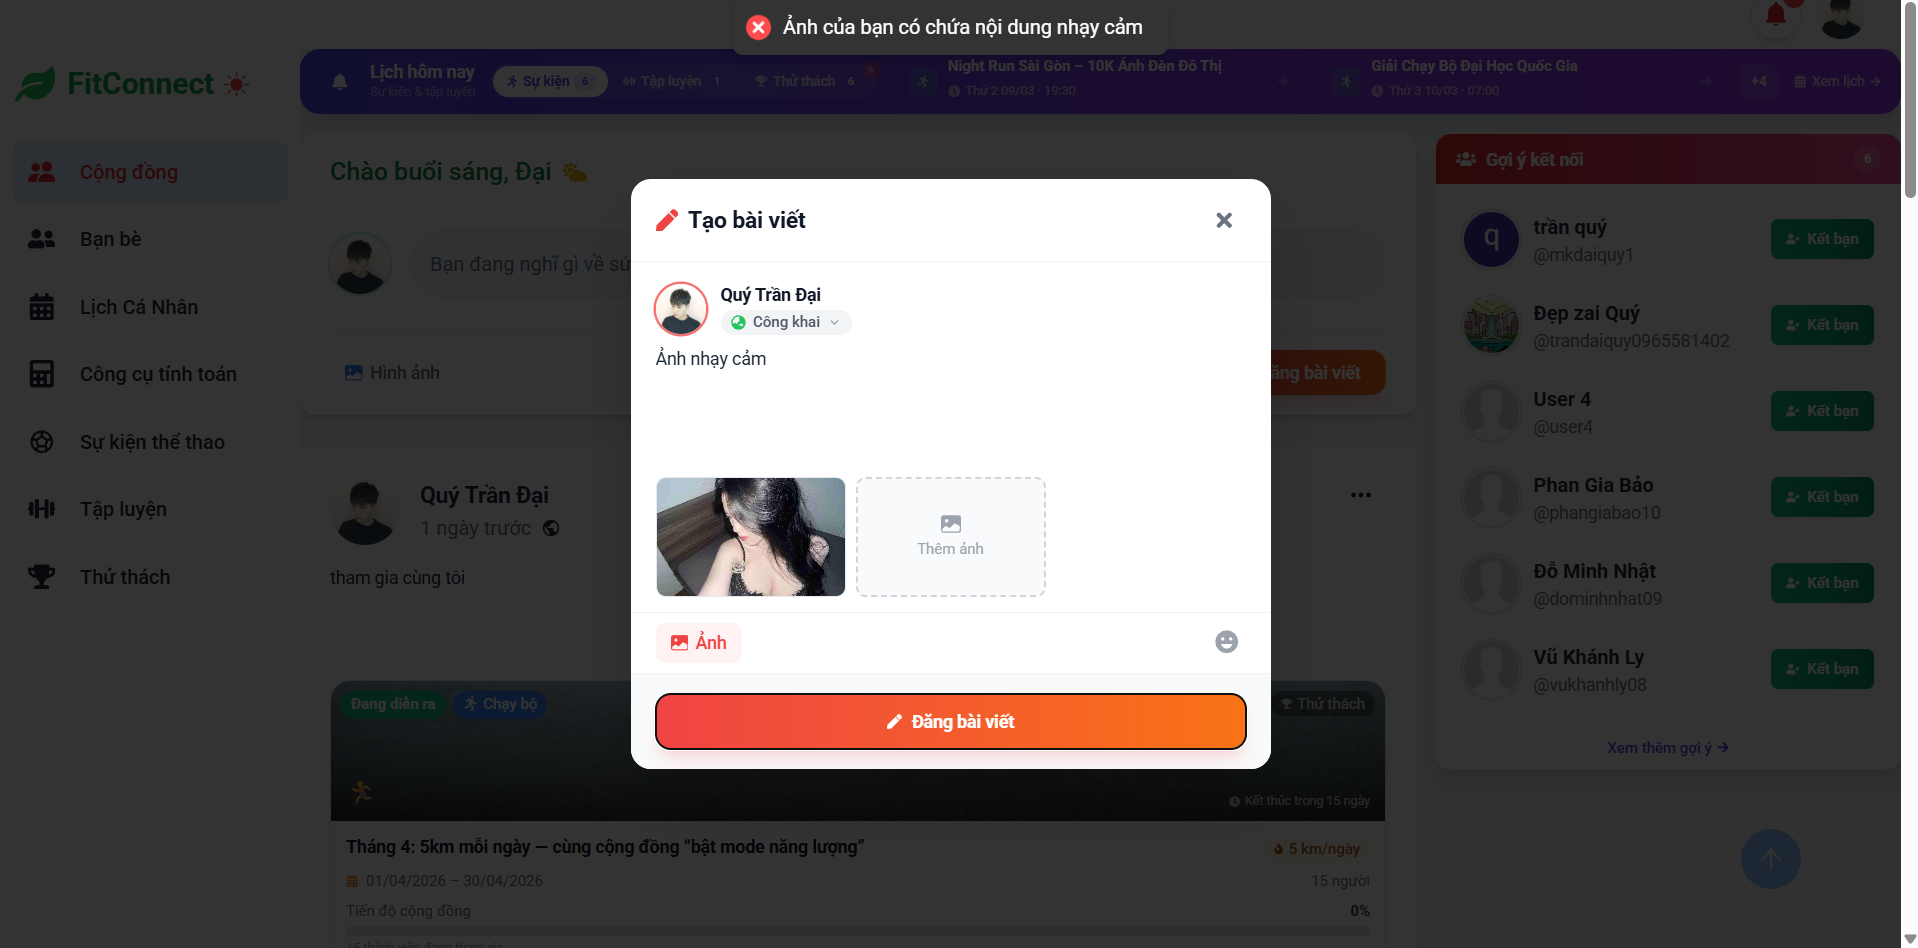
\includegraphics[width=0.60\textwidth]{Images/IMG/CongDong/AInhanbietanhnhaycam.png}
    \caption{Hệ thống AI phát hiện và cảnh báo ảnh nhạy cảm khi người dùng đăng bài}
    \label{fig:impl_ai_nsfw}
\end{figure}

\subsubsection{Lọc từ ngữ nhạy cảm khi đăng bài và bình luận}

Khi người dùng soạn bài viết hoặc gửi bình luận, hệ thống tự động phân tích văn bản bằng mô hình lọc ngôn ngữ theo quy tắc (rule-based). Nếu phát hiện từ hoặc cụm từ vi phạm, hệ thống chặn hành động và hiển thị thông báo lỗi ngay lập tức, ngăn nội dung không phù hợp được đăng lên cộng đồng. Cơ chế áp dụng đồng nhất cho cả bài viết lẫn bình luận.

\begin{figure}[H]
    \centering
    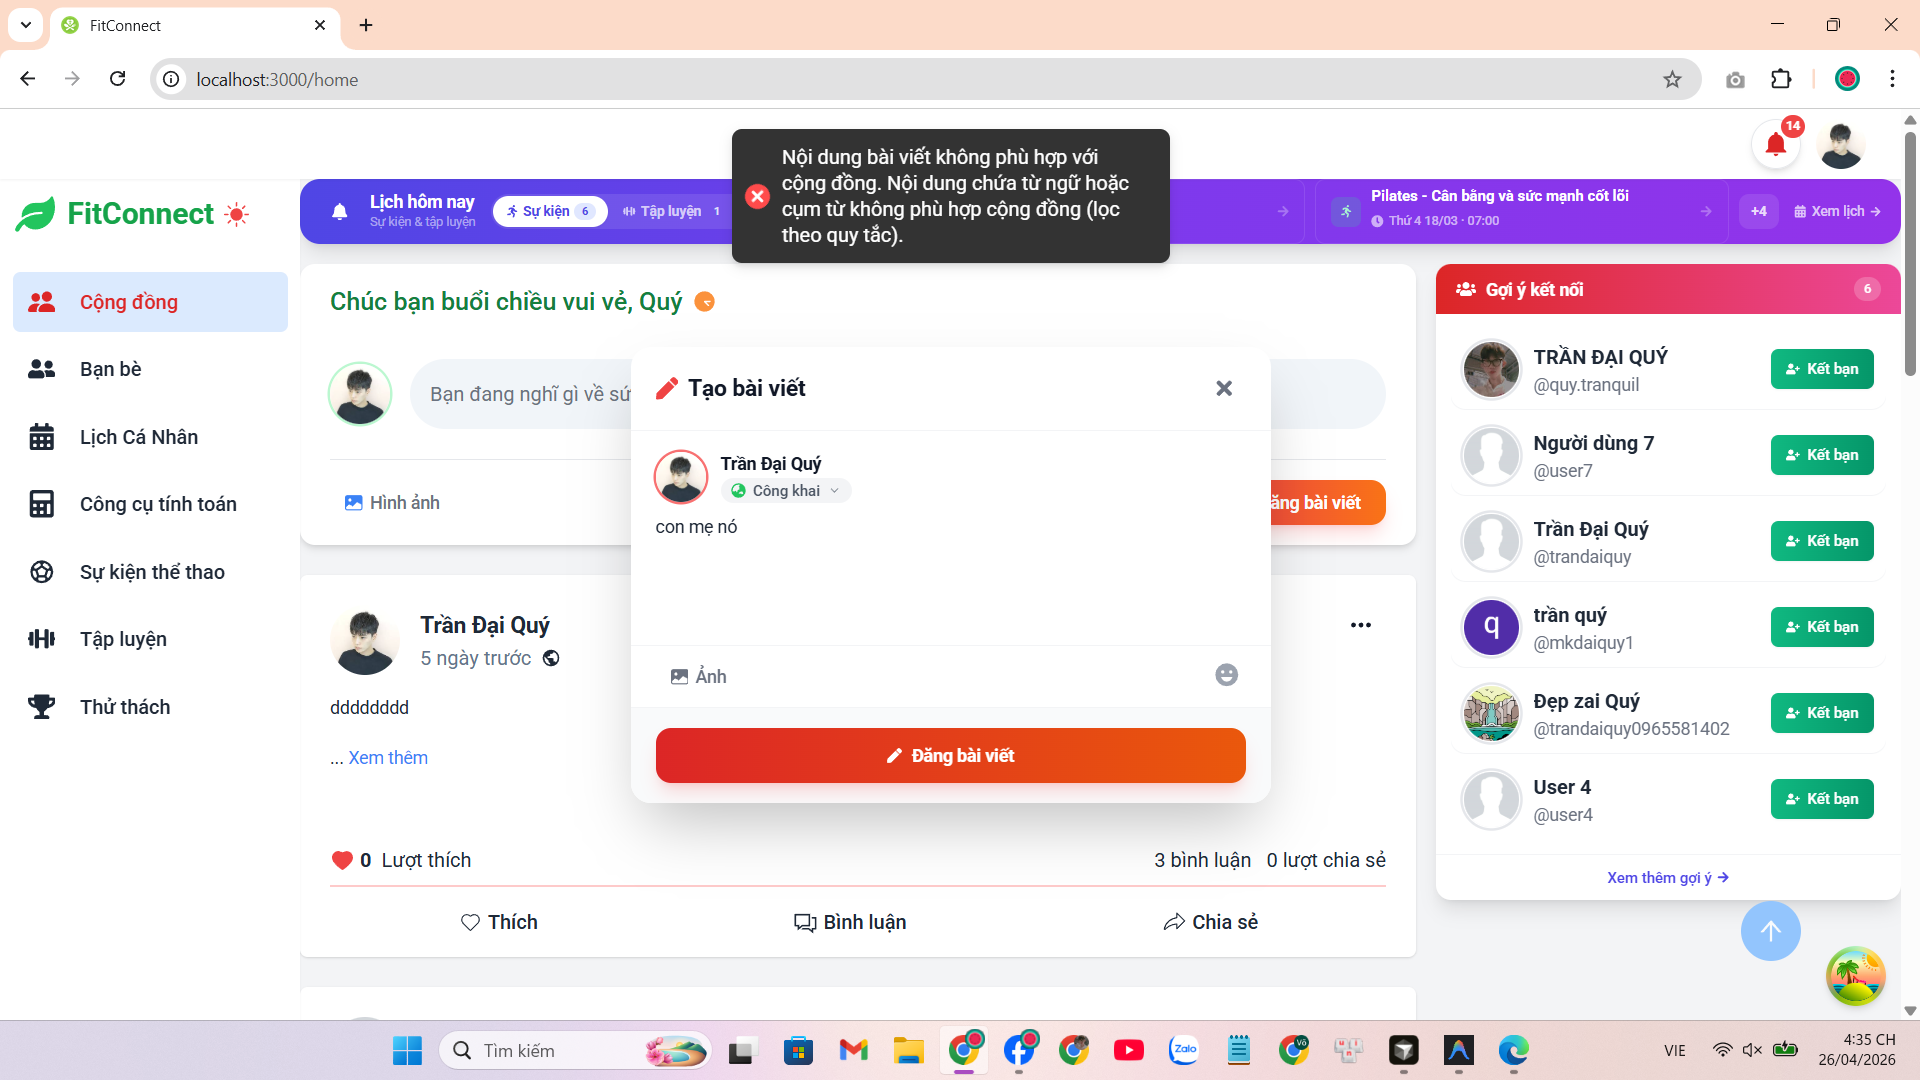
\includegraphics[width=0.60\textwidth]{Images/IMG/Nhom2/dangbainoidungnhaycam.png}
    \caption{Hệ thống phát hiện và chặn đăng bài viết chứa từ ngữ không phù hợp}
    \label{fig:impl_ai_post_filter}
\end{figure}

\subsubsection{Nhận diện khuôn mặt trong phiên Video Call sự kiện trong nhà}

Trong sự kiện thể thao trong nhà, hệ thống dùng TinyFaceDetector (face-api.js) chạy trực tiếp trên trình duyệt để theo dõi sự hiện diện của người tham gia trước camera. Khi phát hiện khuôn mặt, hệ thống hiển thị badge xanh ``AI đang theo dõi'' và tích lũy thời gian tham gia thực tế; khi người dùng rời camera quá lâu, đồng hồ tự dừng và hiển thị trạng thái ``Vắng''.

\begin{figure}[H]
    \centering
    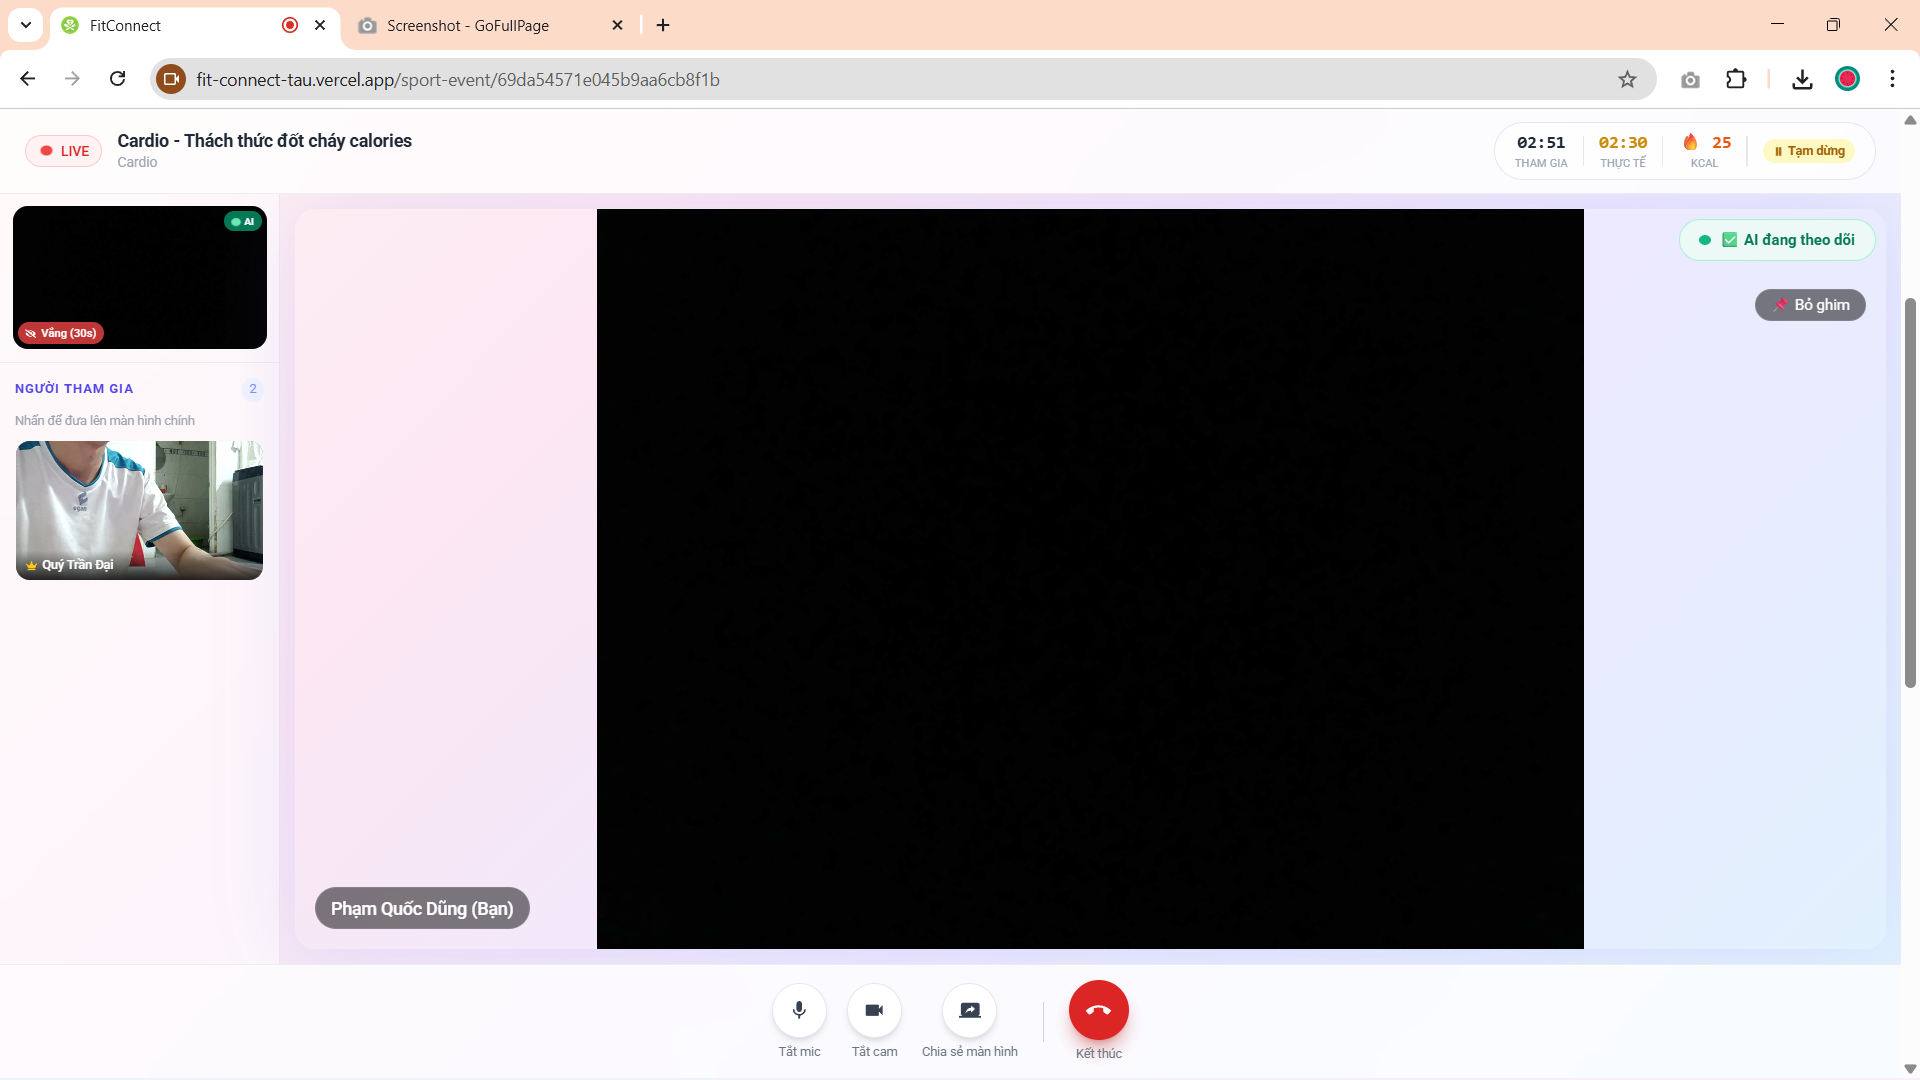
\includegraphics[width=0.60\textwidth]{Images/IMG/nhom3/checameraAInhandientamdung.png}
    \caption{Hệ thống AI nhận diện khuôn mặt và theo dõi sự hiện diện trong phiên Video Call}
    \label{fig:impl_ai_face}
\end{figure}

\subsubsection{Xác minh ảnh bữa ăn trong thử thách ăn uống}

Trong thử thách loại Ăn uống, khi người tham gia check-in bữa ăn bằng ảnh, hệ thống sử dụng AI đa phương thức (thị giác kết hợp ngôn ngữ) để xác minh ảnh có phải bữa ăn hợp lệ theo ngữ cảnh thử thách hay không, trả về ``Ảnh hợp lệ'' (tính tiến độ) hoặc ``Ảnh không phù hợp'' (không tính). Chi tiết tại mục~\ref{subsec:impl_challenge}.

\subsection{Tạo nội dung tự động bằng AI}
\label{subsec:impl_ai_auto_content}

Hệ thống tích hợp AI sinh nội dung (Google Gemini) để giảm thiểu thao tác nhập liệu thủ công trong hai tình huống:

\begin{itemize}
    \item \textbf{Sự kiện thể thao:} Người dùng mô tả ý tưởng bằng ngôn ngữ tự nhiên, AI tự động điền tên, loại sự kiện, địa điểm, thời gian, mô tả chi tiết và ảnh minh họa. Chi tiết tại mục~\ref{subsec:impl_sport_event}.
    \item \textbf{Thử thách cộng đồng:} Chọn loại thử thách (Ngoài trời / Ăn uống / Thể dục) và mô tả ý tưởng; AI điền tên, danh mục, mục tiêu mỗi ngày, thời gian và mô tả. Chi tiết tại mục~\ref{subsec:impl_challenge}.
\end{itemize}

\subsection{Phân tích sức khỏe và gợi ý bài tập cá nhân hóa}
\label{subsec:impl_ai_health_suggest}

Tại trang Công cụ tính toán sức khỏe, sau khi người dùng tính các chỉ số (BMI, TDEE, Body Fat,...), nút ``AI Phân Tích Sức Khỏe'' gửi các chỉ số lên AI để nhận đánh giá tổng quan, lời khuyên dinh dưỡng và danh sách bài tập phù hợp từ kho bài tập hệ thống.

\begin{figure}[H]
    \centering
    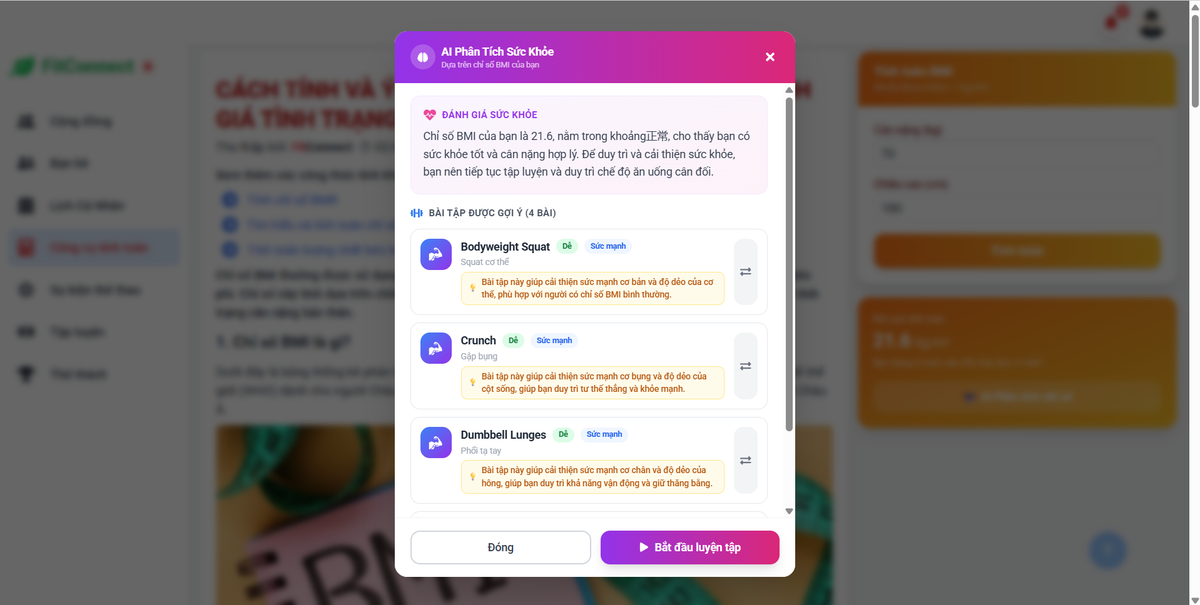
\includegraphics[width=0.60\textwidth]{Images/IMG/Congcusuckhoe/AIphantichsuckhoe.png}
    \caption{Hệ thống AI phân tích sức khỏe và gợi ý bài tập dựa trên chỉ số BMI}
    \label{fig:impl_ai_health}
\end{figure}

Tại trang Tập luyện, tính năng ``AI Gợi ý Tập Luyện'' cho phép người dùng mô tả tình trạng sức khỏe bằng ngôn ngữ tự nhiên (ví dụ: ``Tôi bị đau lưng, gợi ý bài tập phù hợp''). AI kết hợp mô tả với kho bài tập trong CSDL để trả về lời khuyên chi tiết và danh sách bài tập kèm lý do phù hợp. Người dùng chọn bài tập, sắp xếp thứ tự và nhấn ``Bắt đầu luyện tập''.

\begin{figure}[H]
    \centering
    \begin{subfigure}[b]{0.30\textwidth}
        \centering
        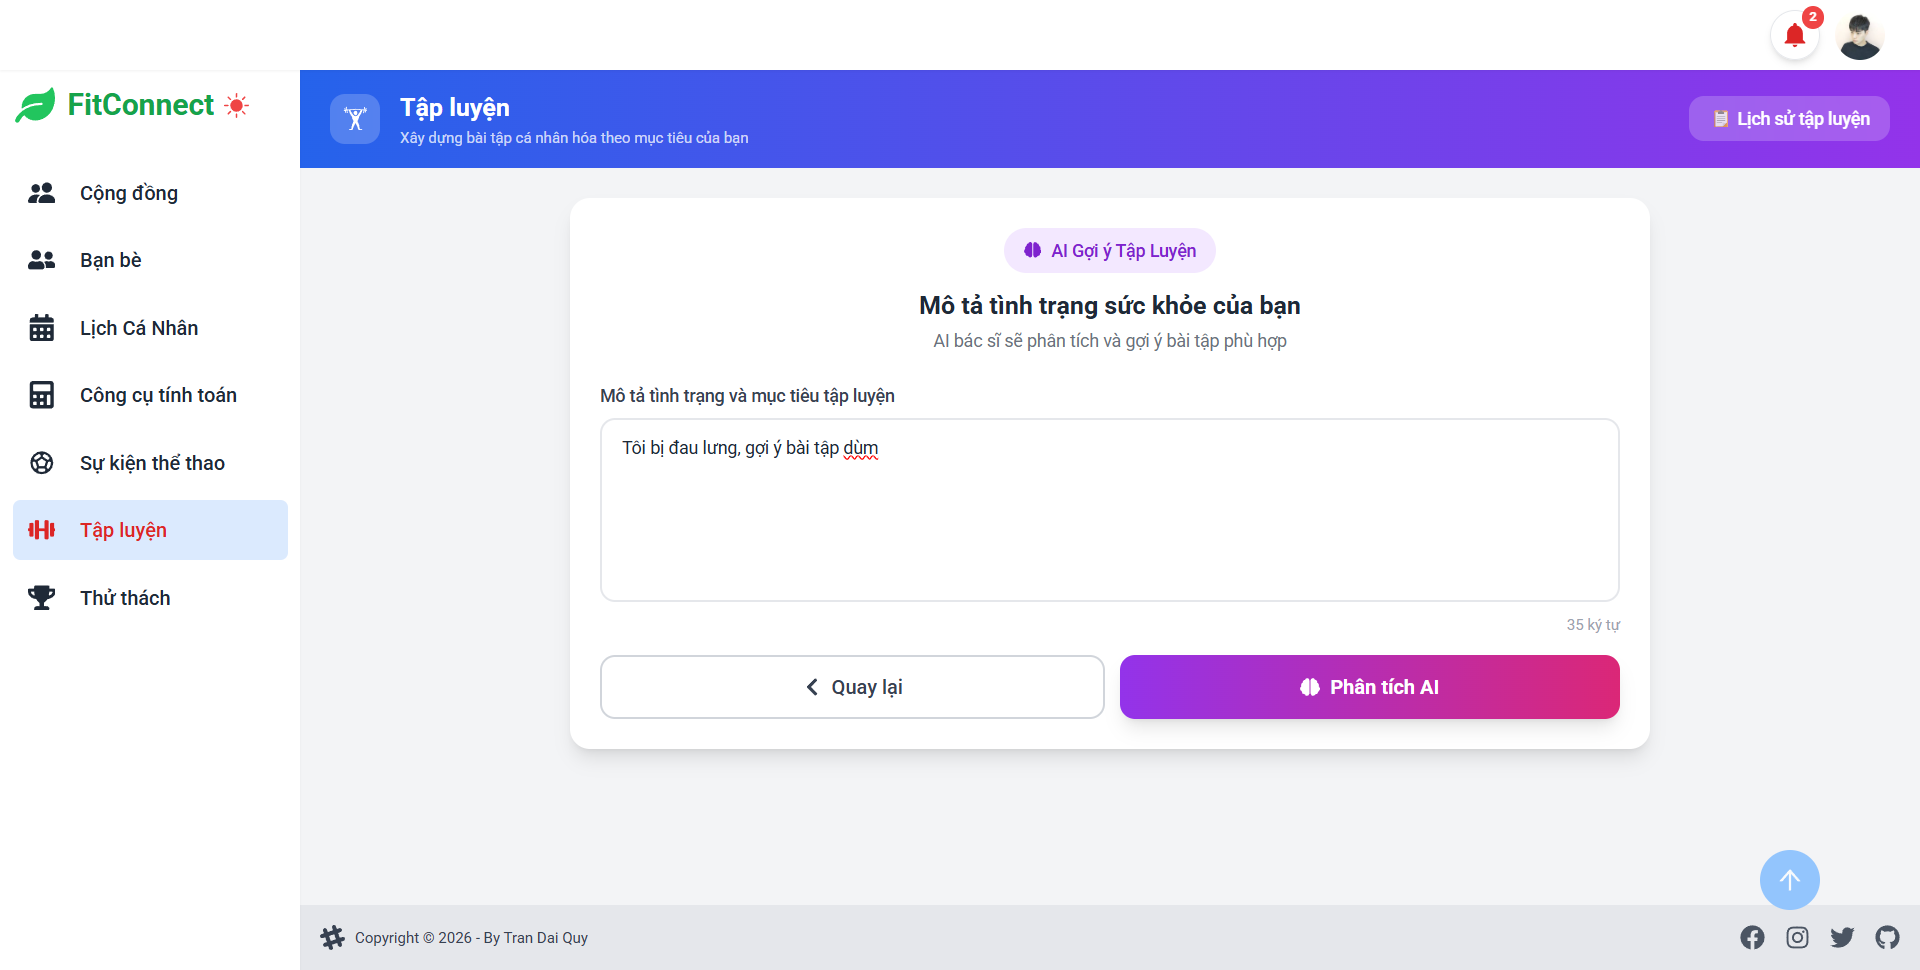
\includegraphics[width=\textwidth]{Images/IMG/Tapluyen/AIgoiytapluyen.png}
        \caption{Người dùng mô tả tình trạng sức khỏe để AI gợi ý bài tập}
        \label{fig:impl_ai_suggest_input}
    \end{subfigure}
    \hfill
    \begin{subfigure}[b]{0.30\textwidth}
        \centering
        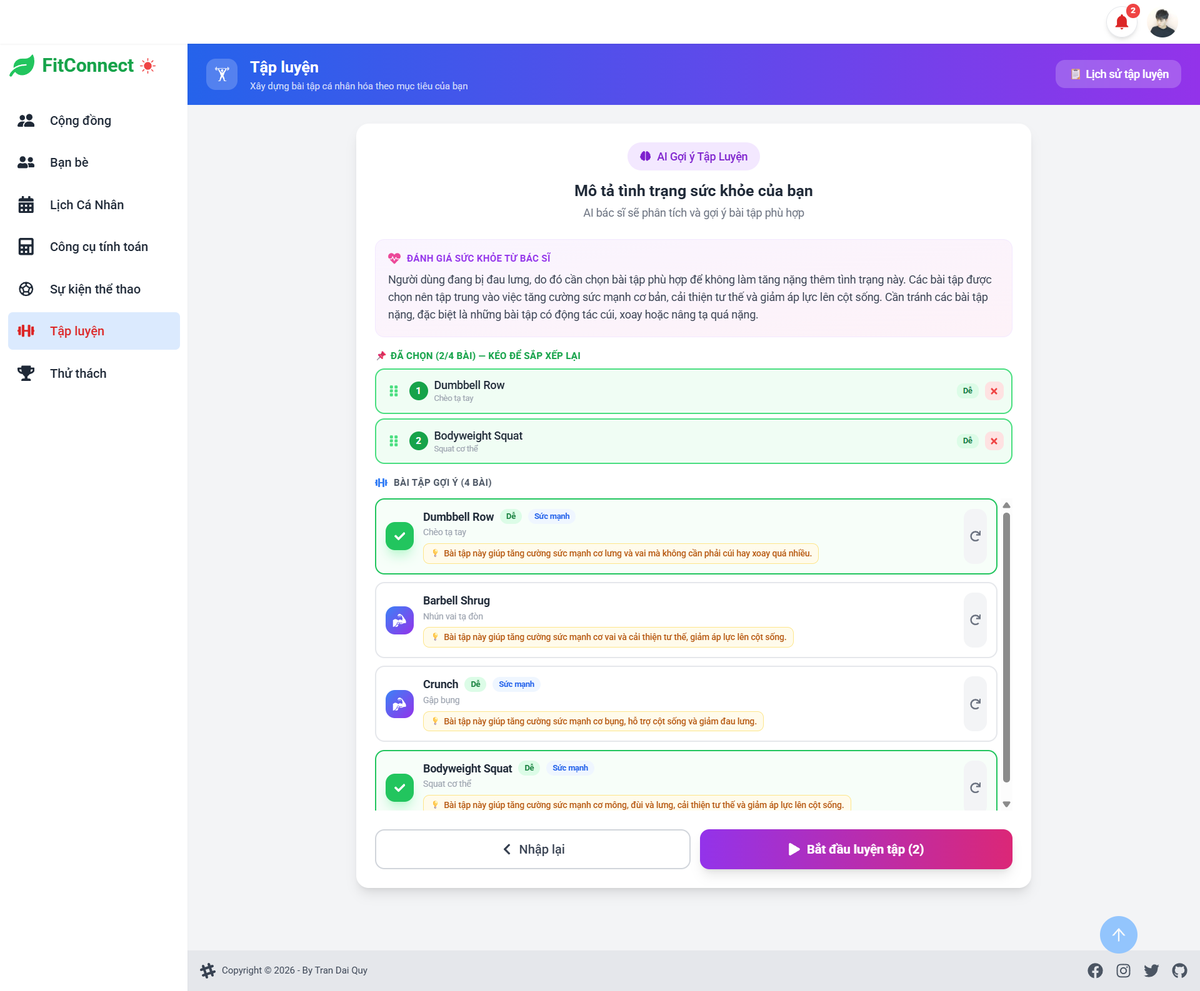
\includegraphics[width=\textwidth]{Images/IMG/Tapluyen/AIgoiytapluyen2.png}
        \caption{Hệ thống AI trả về đánh giá sức khỏe và danh sách bài tập gợi ý}
        \label{fig:impl_ai_suggest_result}
    \end{subfigure}
    \hfill
    \begin{subfigure}[b]{0.30\textwidth}
        \centering
        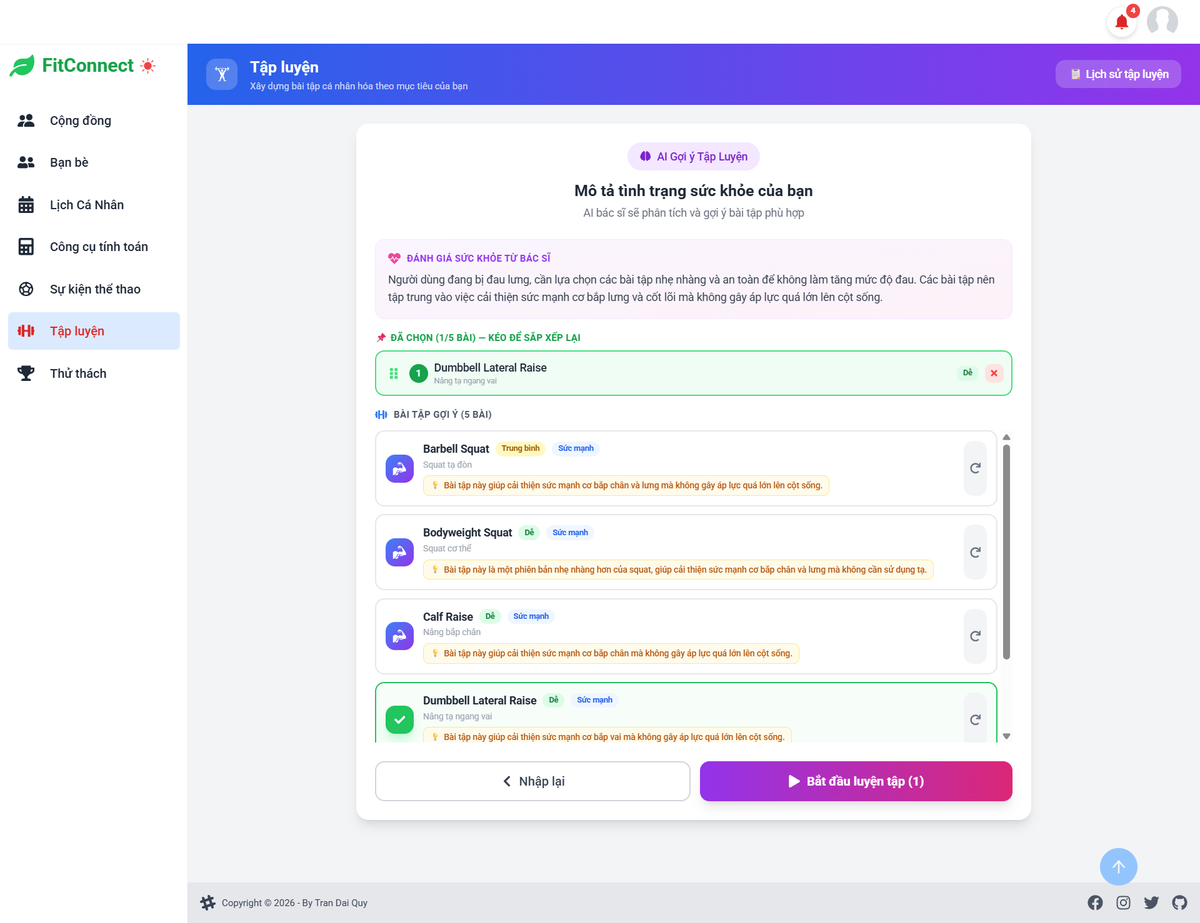
\includegraphics[width=\textwidth]{Images/IMG/nhom5/aigoigoiydanhsachbaitap.png}
        \caption{Người dùng chọn bài tập từ danh sách gợi ý AI và bắt đầu luyện tập}
        \label{fig:impl_ai_suggest_select}
    \end{subfigure}
\end{figure}

\subsection{Ghi nhận và thống kê sử dụng AI}
\label{subsec:impl_ai_usage}

Mọi lần gọi AI thành công đều được hệ thống ghi nhận vào cơ sở dữ liệu (phân loại theo tính năng: tạo sự kiện, tạo thử thách, gợi ý bài tập, xác minh ảnh bữa ăn,...). Dữ liệu này được tổng hợp và hiển thị trên bảng điều khiển Quản trị viên, giúp theo dõi tần suất sử dụng AI theo từng tính năng, đánh giá hiệu quả và tối ưu hóa hệ thống.

\section{Hiện thực các nhóm tính năng}
\label{sec:impl_features}

Hệ thống FitConnect được xây dựng như một hệ sinh thái rèn luyện thể chất toàn diện, bao gồm 9 nhóm tính năng cốt lõi có mối quan hệ tương hỗ chặt chẽ với nhau. Sự kết nối này đảm bảo luồng dữ liệu thông suốt: từ việc định danh người dùng (Account), kết nối cộng đồng (Community, Friends), đến việc tổ chức các hoạt động thi đua (Sport Events, Challenges) và cá nhân hóa lộ trình tập luyện (Training, Health Metrics, AI Suggestions) dựa trên lịch trình thống nhất (Calendar).

Mối quan hệ giữa 9 nhóm tính năng này được thể hiện trực quan qua Hình \ref{fig:impl_feature_overview}, minh chứng cho triết lý thiết kế ``Dữ liệu làm nền tảng -- AI dẫn dắt -- Cộng đồng lan tỏa'' của nền tảng.


\begin{figure}[H]
    \centering
    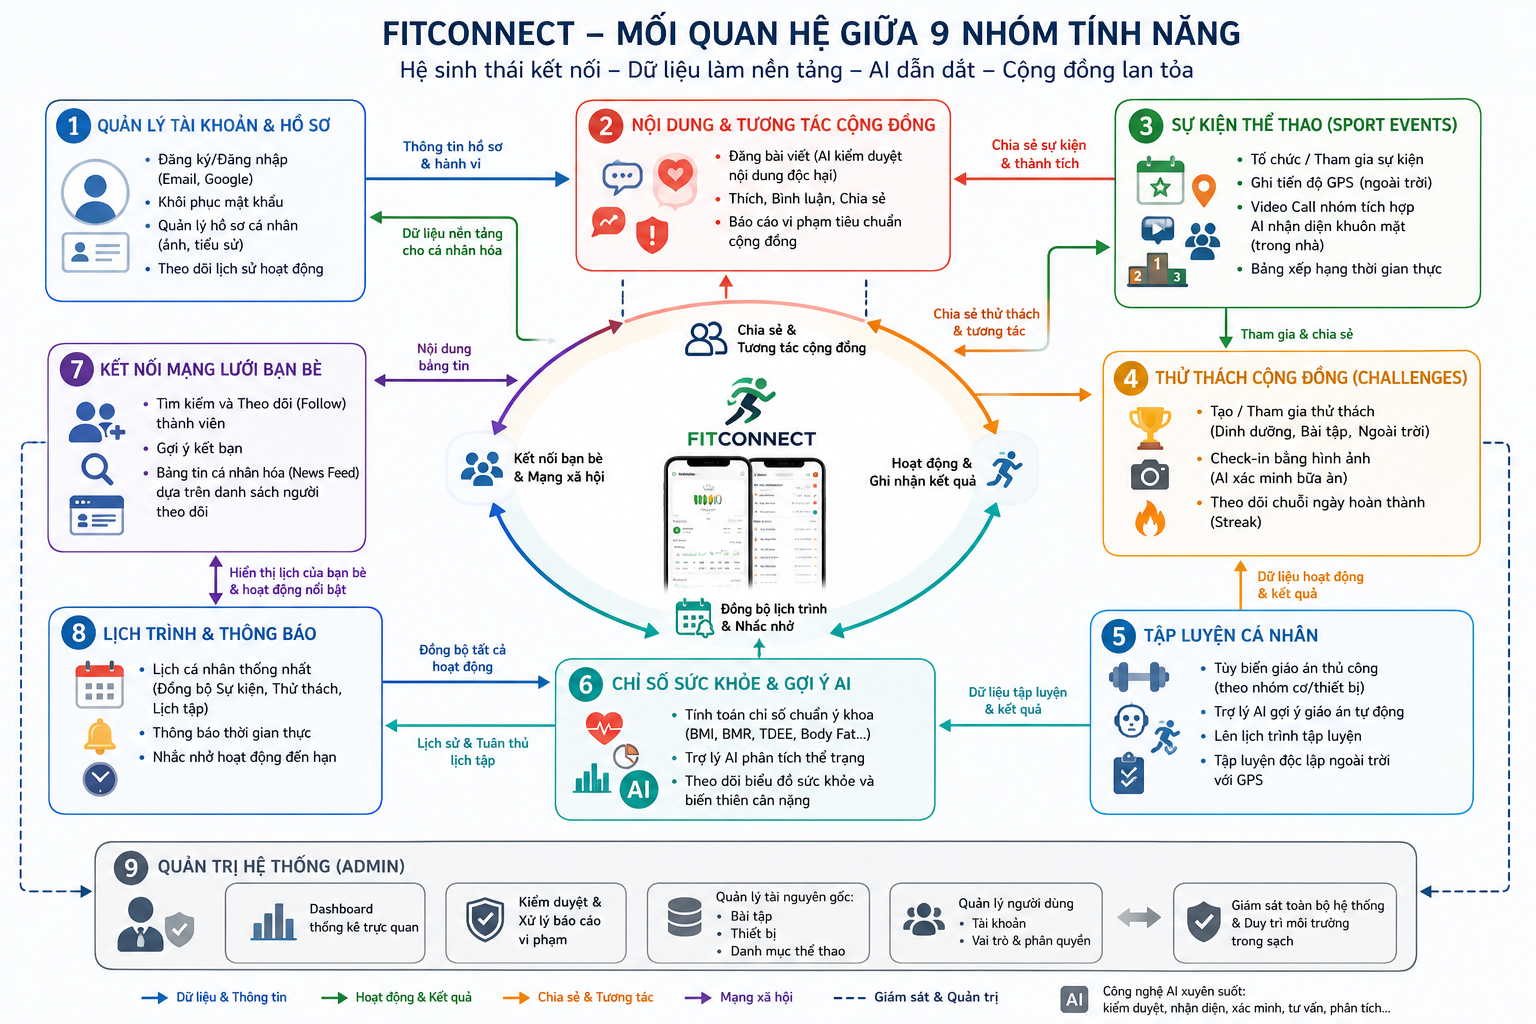
\includegraphics[width=0.60\textwidth]{Images/IMG/Motahethong.png}
    \caption{Sơ đồ tổng quan mối quan hệ tương hỗ giữa 9 nhóm tính năng trong hệ sinh thái FitConnect}
    \label{fig:impl_feature_overview}
\end{figure}


Dưới đây là phần hiện thực chi tiết kết quả của từng nhóm tính năng cốt lõi cấu thành hệ thống. Mỗi tính năng được phân tích theo \textbf{Luồng xử lý (Workflow)} kết hợp kiến trúc kỹ thuật và minh họa trực quan từ giao diện ứng dụng thực tế.

\subsection{Nhóm tính năng Quản lý Tài khoản \& Hồ sơ (Account \& Profile)}
\label{subsec:impl_account}

Đây là nhóm chức năng đóng vai trò định danh, cá nhân hóa không gian hoạt động của người dùng, và bảo mật quyền truy cập toàn rải hệ thống. Quá trình hoạt động được chia thành 3 luồng chính.

\subsubsection{Luồng Đăng ký và Đăng nhập hệ thống}
\textbf{Mục tiêu:} Kiểm soát quyền truy cập qua cơ chế JWT, ngăn chặn tấn công giả mạo và cung cấp khả năng Login nhanh thông qua hệ sinh thái Google.
\textbf{Luồng xử lý kỹ thuật:}
\begin{enumerate}
    \item \textbf{Đăng ký tài khoản (Hình \ref{fig:impl_register}):} Người dùng cung cấp thư điện tử (Email), mật khẩu và các thông tin cơ bản. Ứng dụng tiến hành kiểm tra tính hợp lệ của dữ liệu đầu vào theo thời gian thực trước khi gửi yêu cầu đến máy chủ. Tại phía máy chủ, thông tin xác thực được xử lý bằng thuật toán băm (Hash) kết hợp kỹ thuật thêm chuỗi ngẫu nhiên (Salt) nhằm đảm bảo an toàn tuyệt đối trước khi lưu trữ vào cơ sở dữ liệu.
    \item \textbf{Đăng nhập và định danh (Hình \ref{fig:impl_login}):} Quá trình đăng nhập hỗ trợ hai phương thức: xác thực truyền thống qua thư điện tử và xác thực bên thứ ba thông qua hệ sinh thái Google (OAuth 2.0). Khi định danh thành công, hệ thống cấp phát một chứng thư số điện tử dạng mã thông báo (Access Token) có thời hạn sử dụng xác định. Chứng thư này được ứng dụng phía máy khách lưu giữ và đính kèm tự động vào thao tác giao tiếp tiếp theo để duy trì trạng thái phiên hoạt động.
\end{enumerate}


\begin{figure}[H]
    \centering
    \begin{subfigure}[b]{0.30\textwidth}
        \centering
        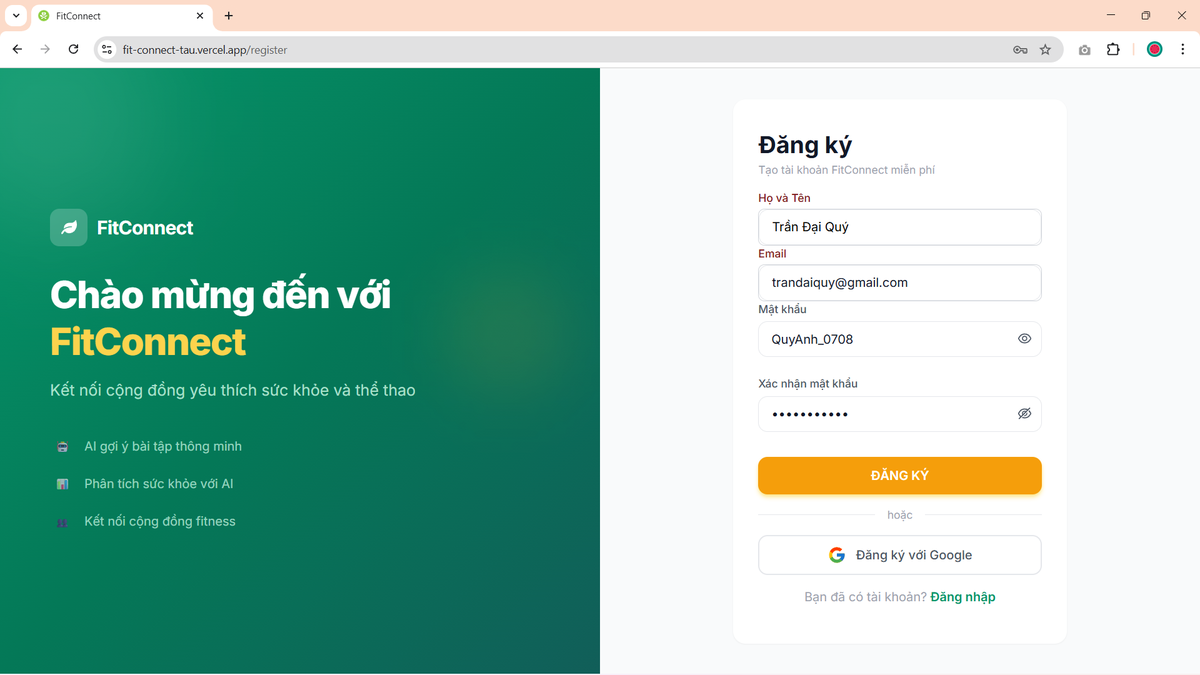
\includegraphics[width=\textwidth]{Images/IMG/Nhom1/dangky.png}
        \caption{Giao diện Đăng ký thành viên FitConnect}
        \label{fig:impl_register}
    \end{subfigure}
    \hfill
    \begin{subfigure}[b]{0.30\textwidth}
        \centering
        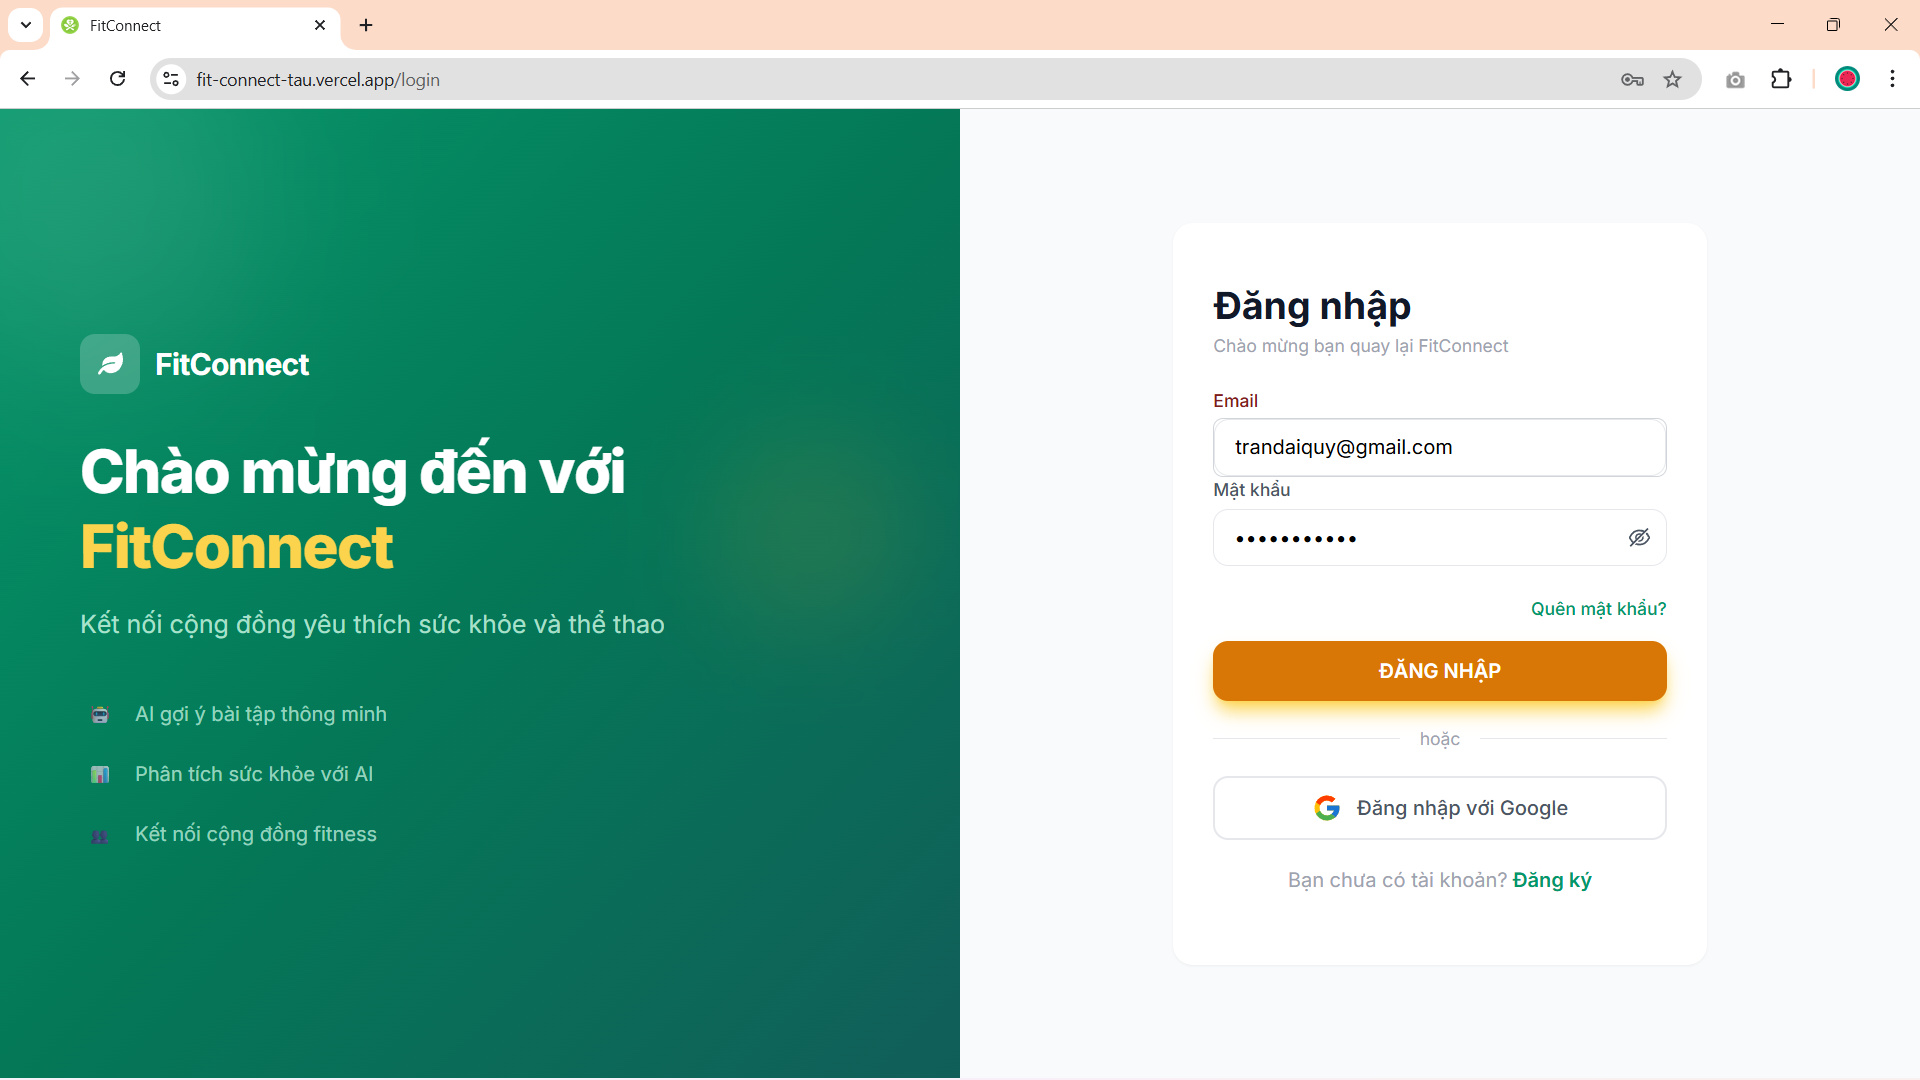
\includegraphics[width=\textwidth]{Images/IMG/Nhom1/dangnhap.png}
        \caption{Giao diện Đăng nhập hệ thống}
        \label{fig:impl_login}
    \end{subfigure}
    \hfill
    \begin{subfigure}[b]{0.30\textwidth}
        \centering
        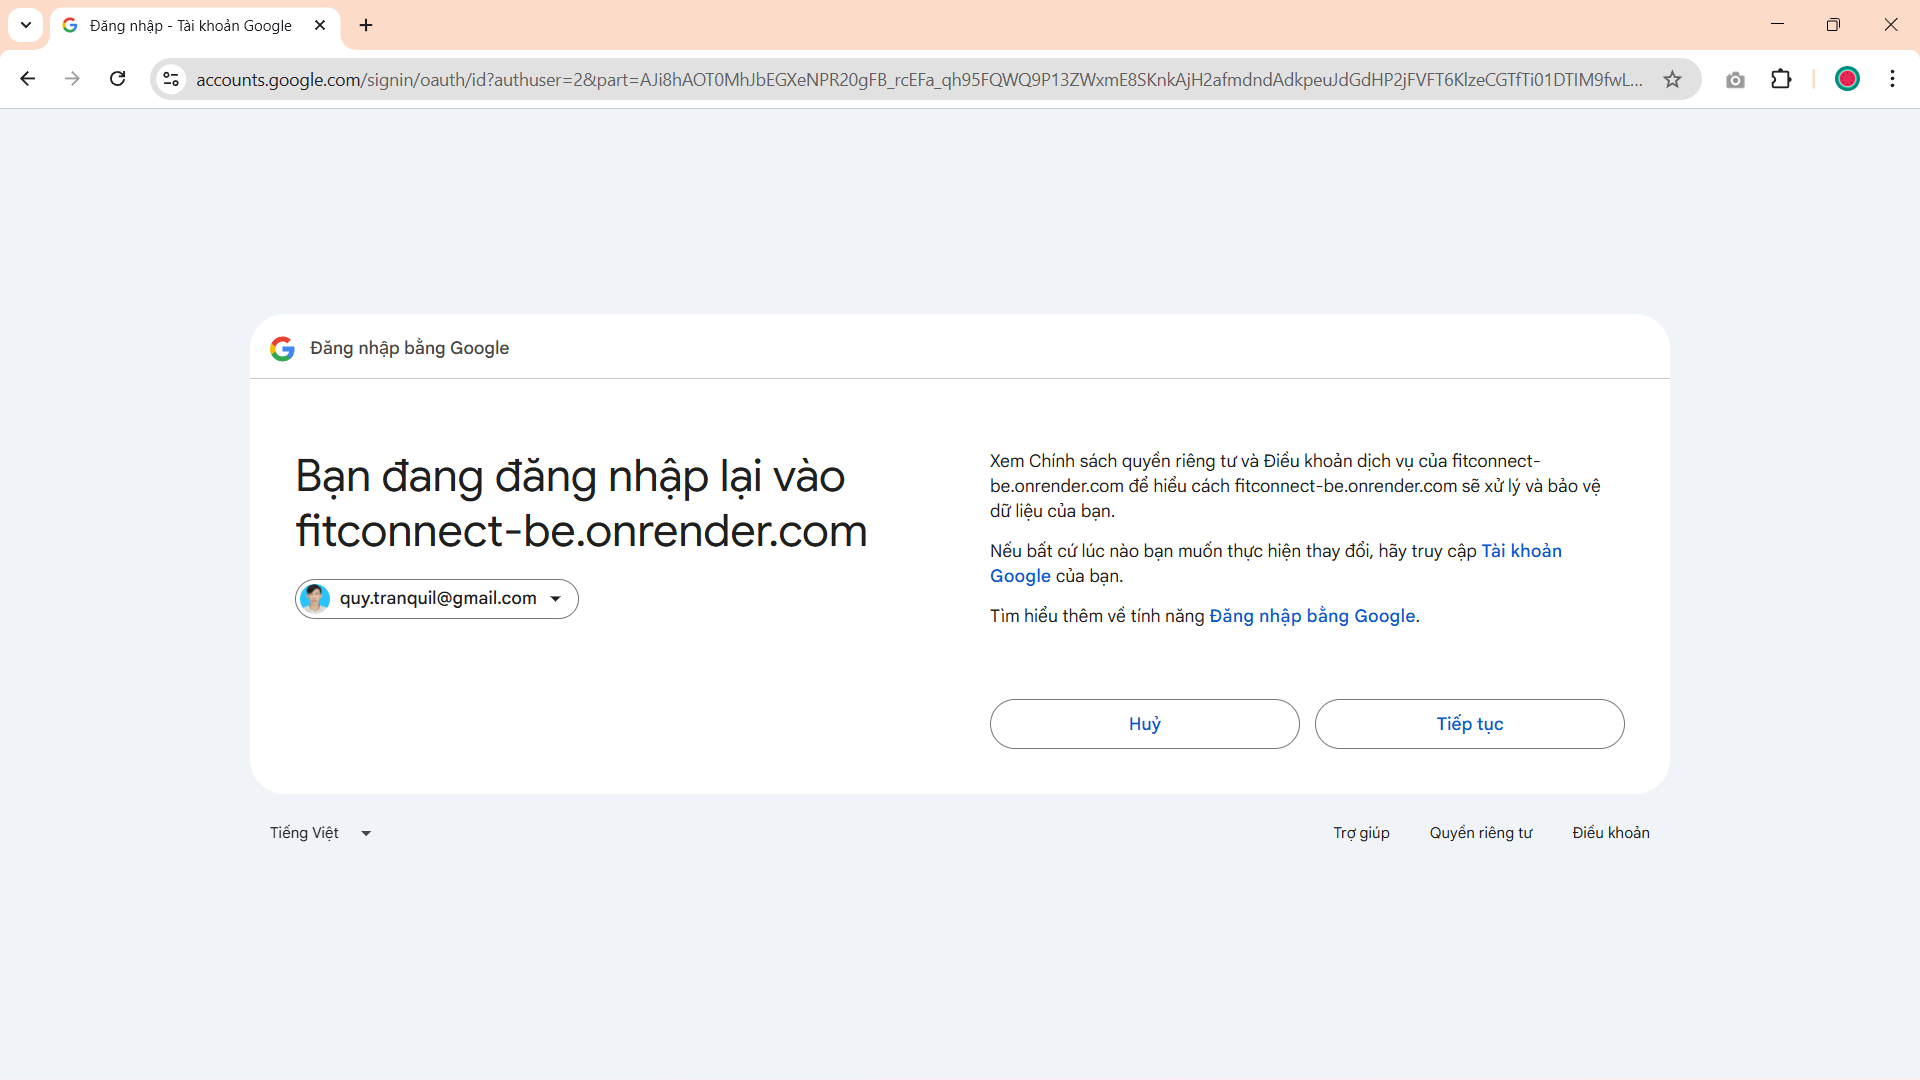
\includegraphics[width=\textwidth]{Images/IMG/Nhom1/logingoogle.png}
        \caption{Lựa chọn Xác thực tài khoản nhanh qua Google OAuth}
        \label{fig:impl_login_google}
    \end{subfigure}
\end{figure}

Sau khi xác thực thành công, hệ thống cấp phát Access Token và tự động điều hướng người dùng về Trang chủ (Home) với bảng tin cộng đồng.


\subsubsection{Luồng Xác thực OTP và Khôi phục mật khẩu}
\textbf{Mục tiêu:} Hỗ trợ người dùng khôi phục quyền truy cập tài khoản một cách an toàn thông qua quy trình xác minh hai bước bằng mã sử dụng một lần (OTP - One-Time Password) gửi qua thư điện tử.
\textbf{Quy trình hoạt động:}
\begin{enumerate}
    \item \textbf{Yêu cầu thiết lập lại (Hình \ref{fig:impl_forgot_pw}):} Hệ thống tiếp nhận thư điện tử do người dùng cung cấp và đối chiếu với cơ sở dữ liệu. Nếu tài khoản khả dụng, một mã xác thực OTP ngẫu nhiên gồm 6 chữ số sẽ được khởi tạo với vòng đời được quản lý nghiêm ngặt trong 5 phút.
    \item \textbf{Điều phối thư điện tử (Hình \ref{fig:impl_send_otp}):} Thông qua dịch vụ gửi đám mây chuyên dụng, hệ thống tự động biên dịch và gửi thông điệp chứa mã bảo mật đến địa chỉ người dùng cung cấp.
    \item \textbf{Xác thực mã (Hình \ref{fig:impl_input_otp}):} Người dùng điền chuỗi mã gửi về vào giao diện ứng dụng. Hệ thống đối chiếu dữ liệu một cách trực tiếp với mã tại máy chủ; nếu hợp lệ, phiên làm việc sẽ được phê duyệt giới hạn để chuyển sang chặng thay đổi khóa.
    \item \textbf{Tạo mới mật khẩu (Hình \ref{fig:impl_forgot_pw_change}):} Ở thao tác cuối, người dùng tự ấn định một mật khẩu mới. Chuỗi thông tin này bắt buộc chạy qua quy trình băm độc lập trước khi đẩy lùi mật khẩu cũ để tái thiết lập rào chắn bảo vệ của hồ sơ.
\end{enumerate}


\begin{figure}[H]
    \centering
    \begin{subfigure}[b]{0.30\textwidth}
        \centering
        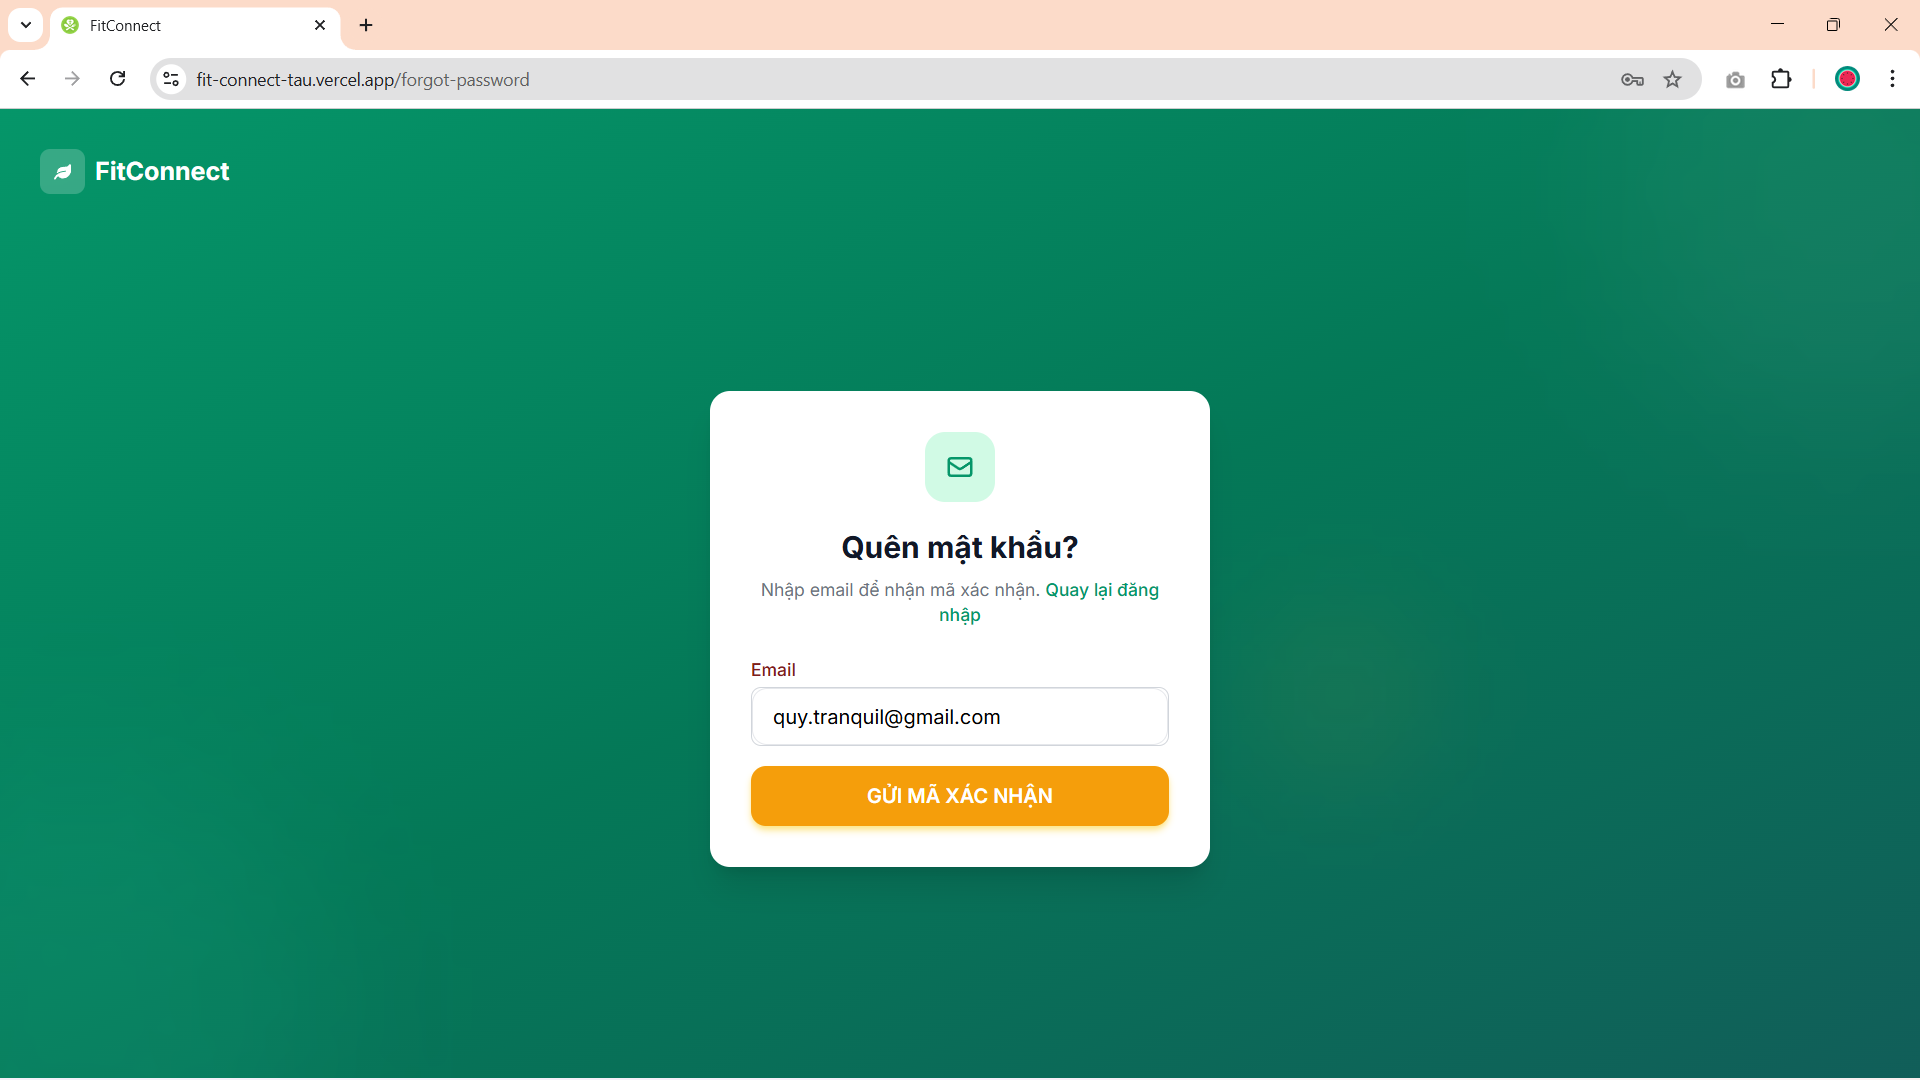
\includegraphics[width=\textwidth]{Images/IMG/Nhom1/quenmatkhau.png}
        \caption{Giao diện điền thông tin Yêu cầu khôi phục mật khẩu}
        \label{fig:impl_forgot_pw}
    \end{subfigure}
    \hfill
    \begin{subfigure}[b]{0.30\textwidth}
        \centering
        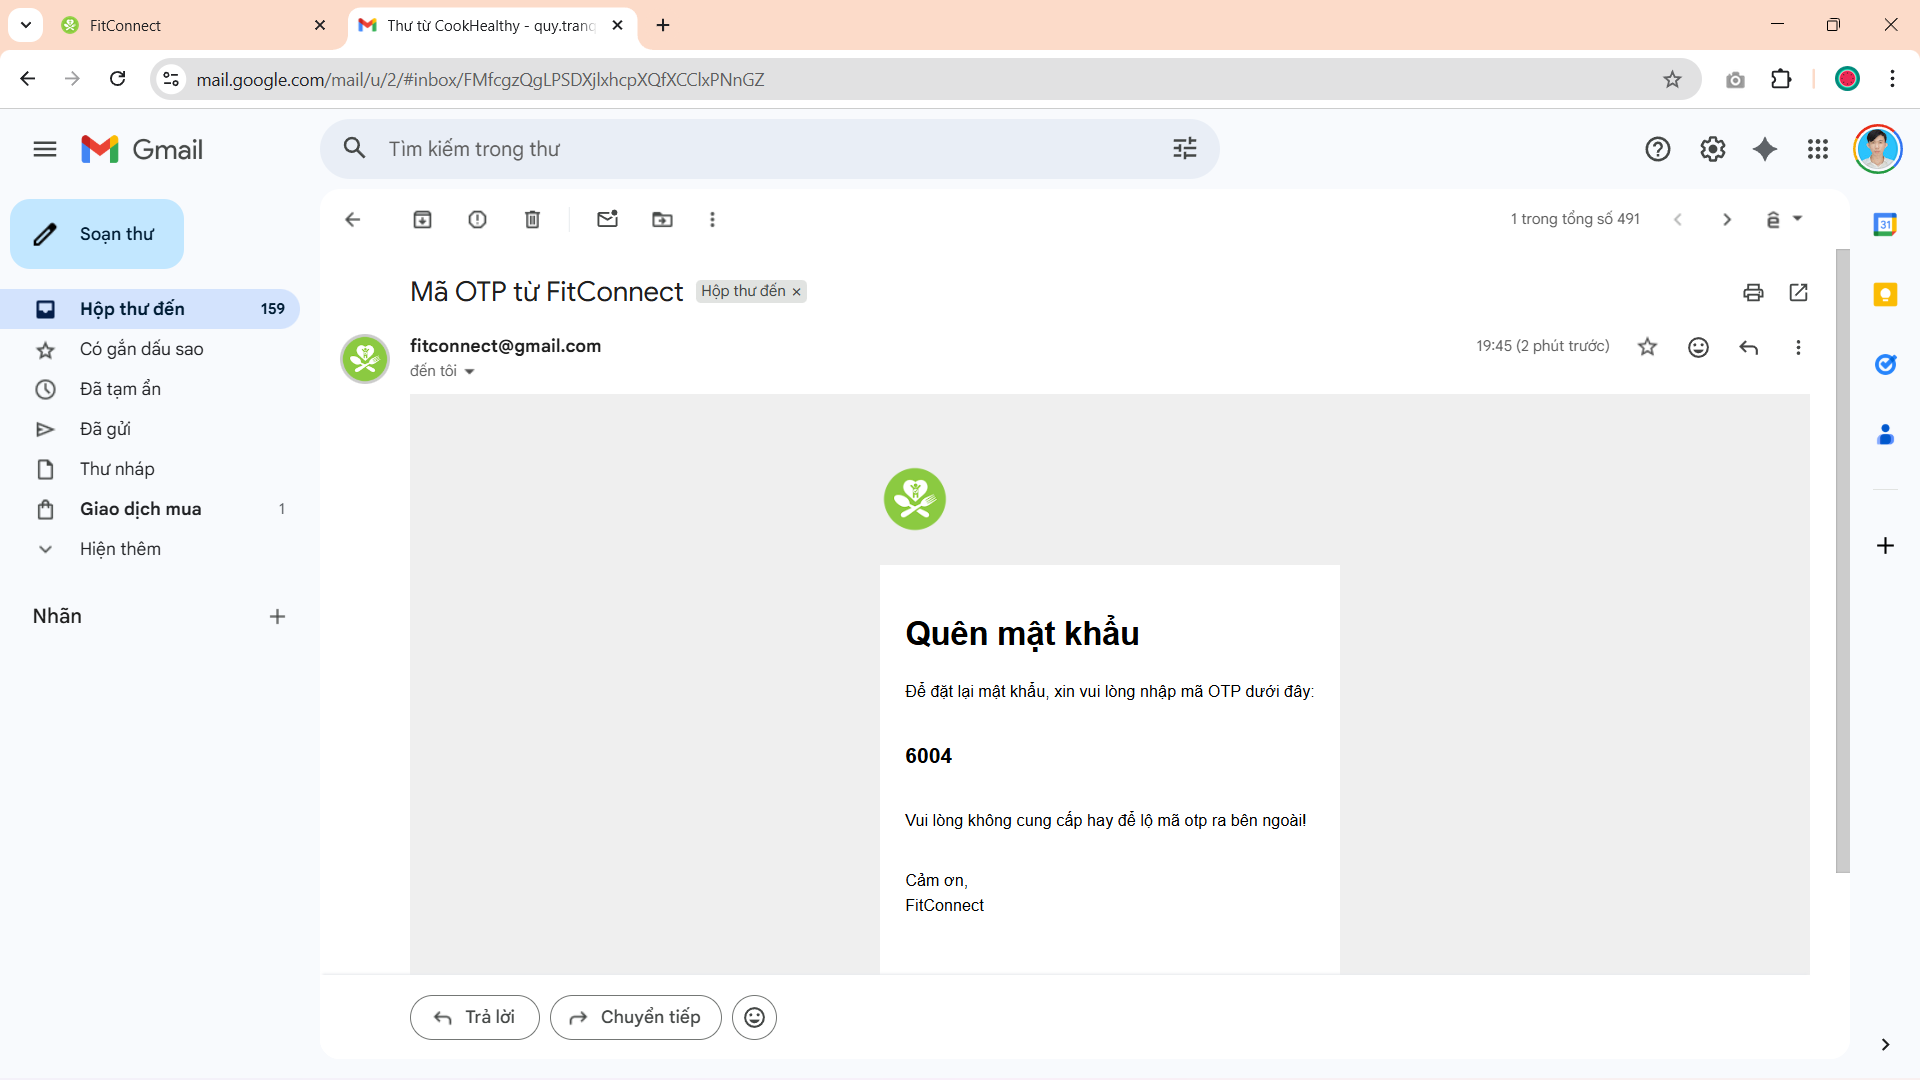
\includegraphics[width=\textwidth]{Images/IMG/Nhom1/guiotpveemail.png}
        \caption{Email tự động gửi dải mã OTP bảo mật 6 ký tự}
        \label{fig:impl_send_otp}
    \end{subfigure}
    \hfill
    \begin{subfigure}[b]{0.30\textwidth}
        \centering
        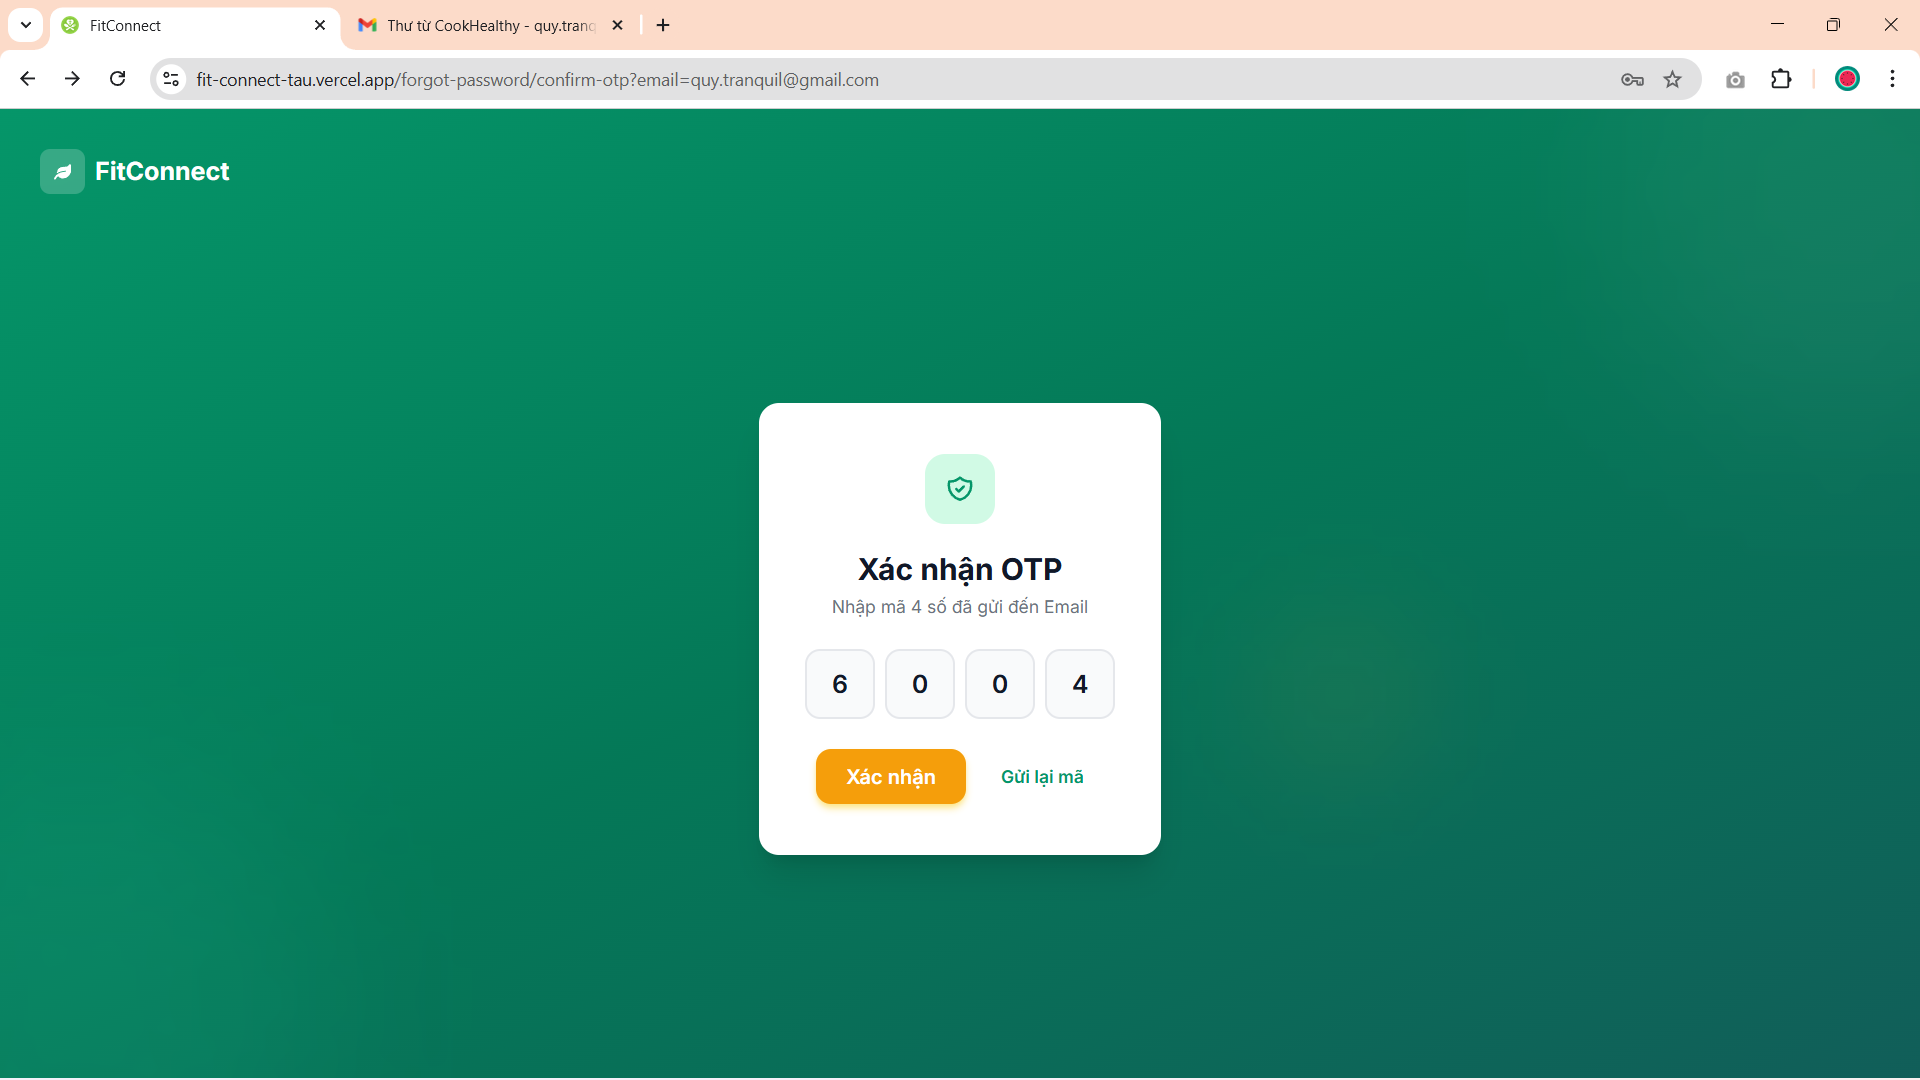
\includegraphics[width=\textwidth]{Images/IMG/Nhom1/nhapotp.png}
        \caption{Giao diện Frontend yêu cầu nhập mã OTP hợp lệ}
        \label{fig:impl_input_otp}
    \end{subfigure}
\end{figure}

\begin{figure}[H]
    \centering
    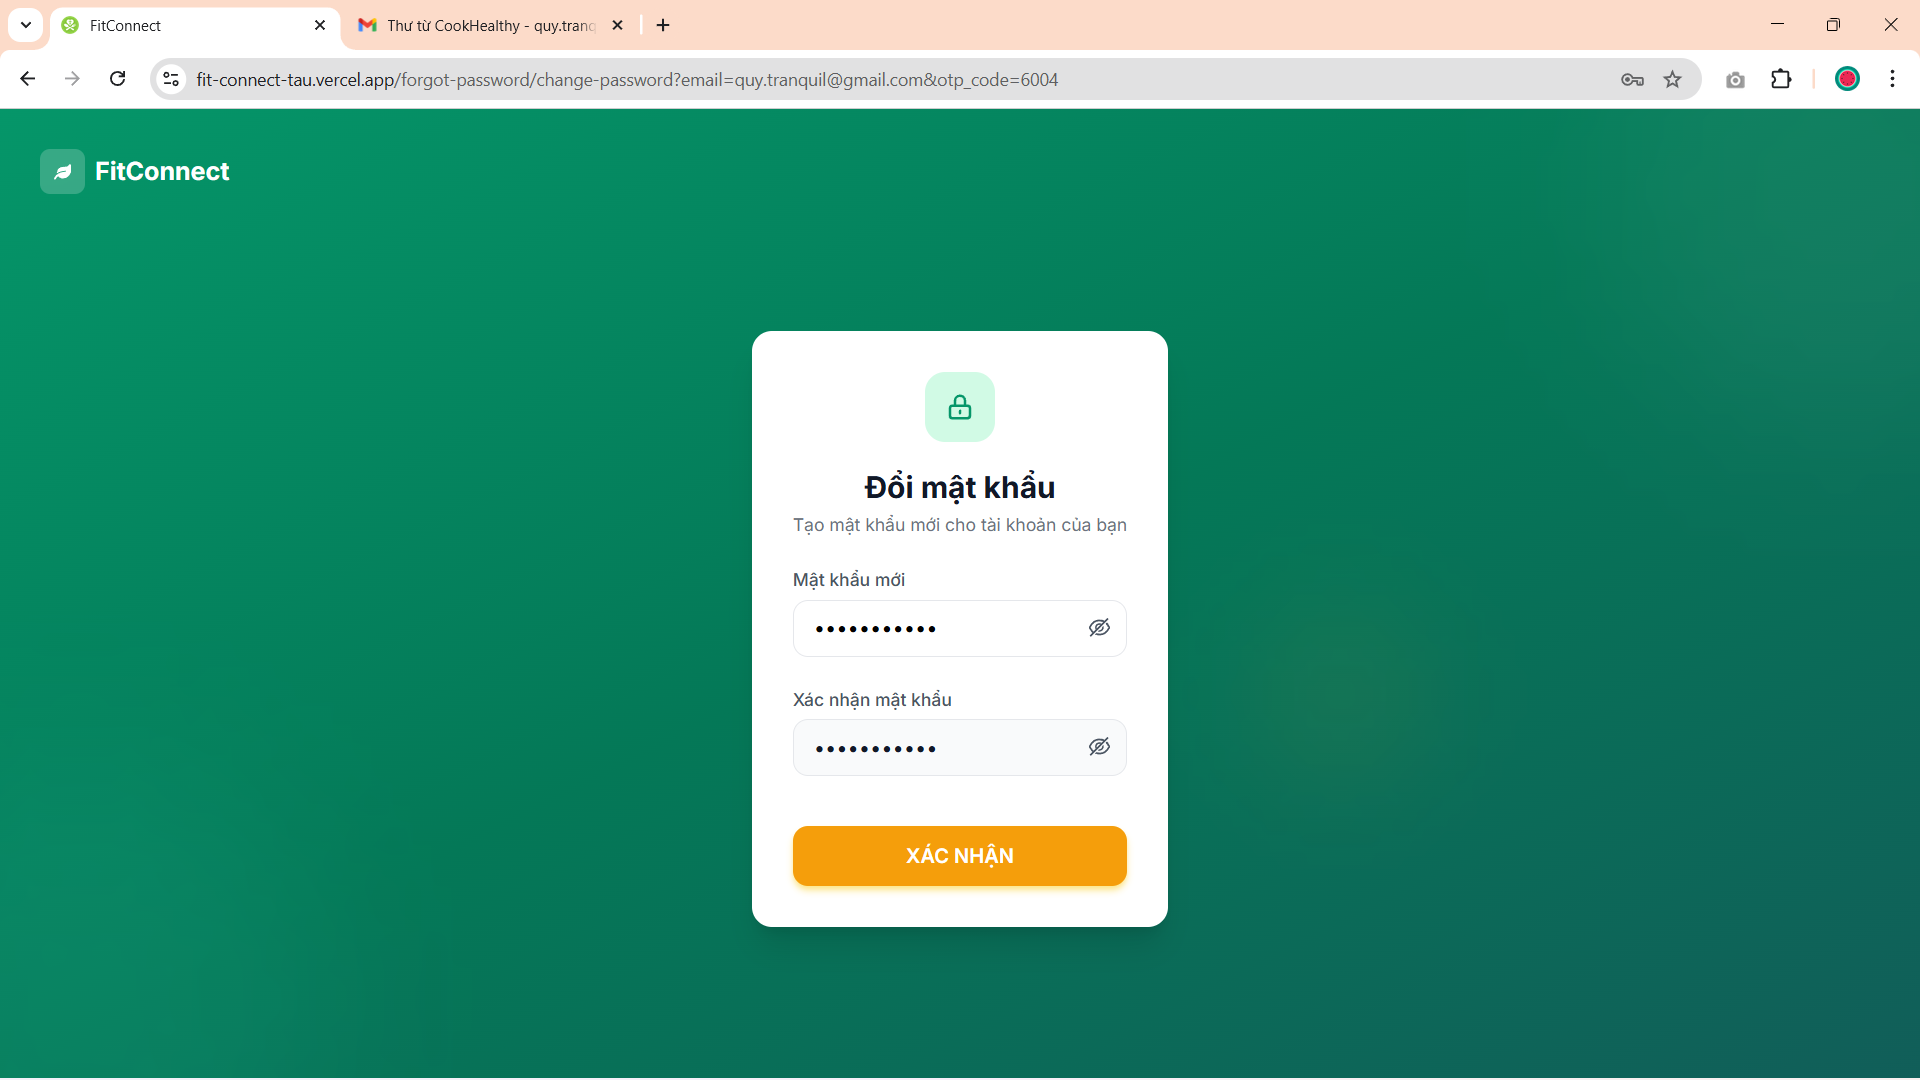
\includegraphics[width=0.60\textwidth]{Images/IMG/Nhom1/doimatkhau.png}
    \caption{Thiết lập mật khẩu mới và khôi phục quyền bảo vệ hoàn tất}
    \label{fig:impl_forgot_pw_change}
\end{figure}



\subsubsection{Luồng Quản trị Hồ sơ \& Tương tác cá nhân hóa (Profile Dashboard)}
\textbf{Mục tiêu:} Xây dựng không gian Profile Dashboard làm trung tâm quản trị hồ sơ cá nhân, nơi người dùng vừa theo dõi tổng quan hoạt động, vừa thực hiện các thao tác cá nhân hóa (ảnh đại diện, ảnh nền, thông tin hồ sơ, bảo mật tài khoản) ngay tại chỗ với số bước tối thiểu.

\textbf{Quy trình hoạt động:}
\begin{itemize}
    \item Người dùng truy cập trang cá nhân để xem thông tin hồ sơ tổng quát (ảnh đại diện, ảnh nền, mô tả, các chỉ số hoạt động). Đây là điểm vào chính của luồng quản trị hồ sơ và các thao tác cá nhân hóa.

\begin{figure}[H]
    \centering
    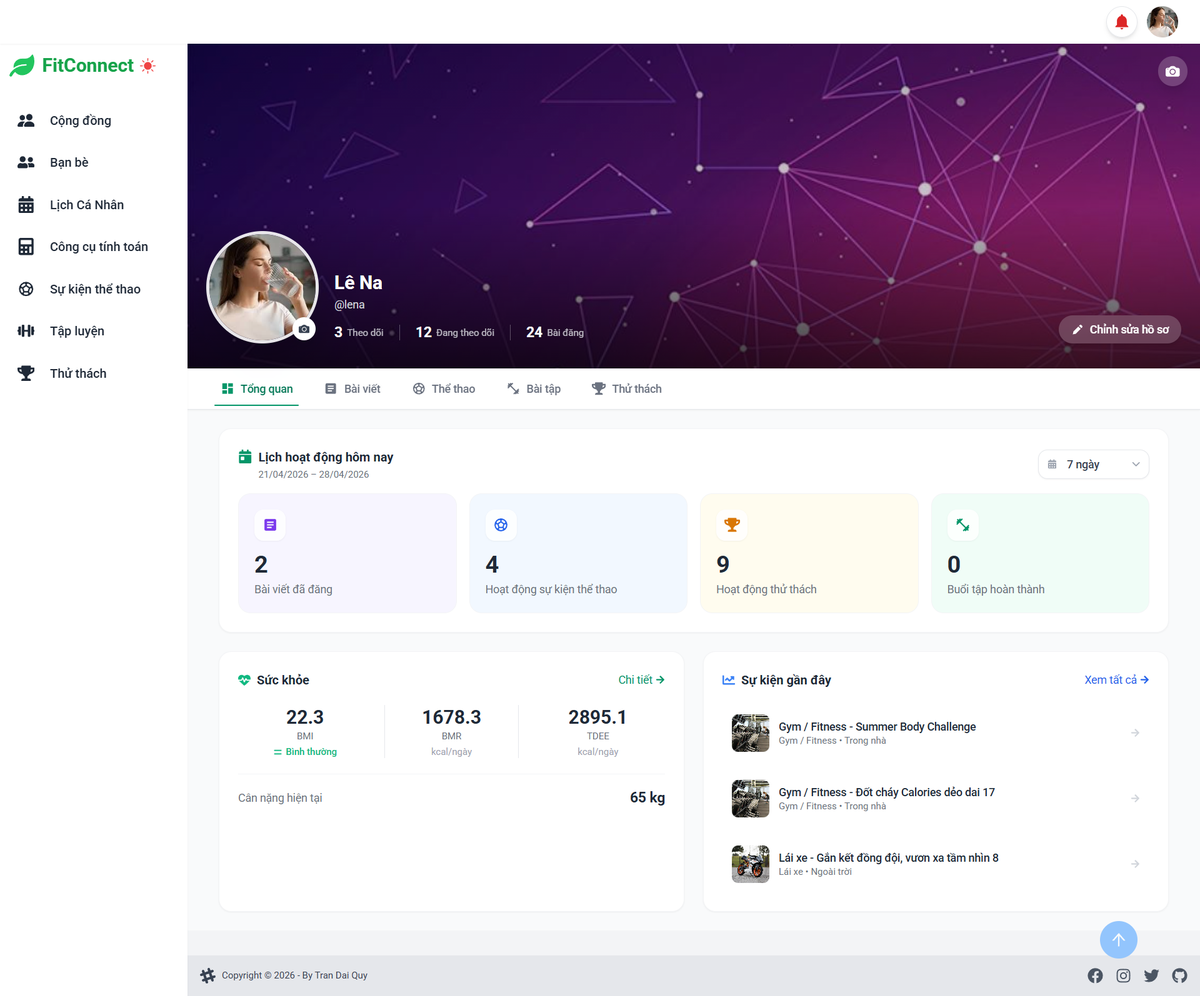
\includegraphics[width=0.60\textwidth]{Images/IMG/Nhom1/trangcanhan.png}
    \caption{Giao diện tổng quan trang cá nhân của người dùng}
    \label{fig:impl_profile_overview}
\end{figure}


    \item Trang cá nhân cung cấp ba tab chuyên biệt để theo dõi hoạt động: tab \textbf{Bài viết} hiển thị lịch sử bài đã đăng, tab \textbf{Sự kiện} tổng hợp sự kiện đã tham gia/tạo, và tab \textbf{Thử thách} tập trung mục tiêu và tiến độ hoàn thành.

\begin{figure}[H]
    \centering
    \begin{subfigure}[b]{0.30\textwidth}
        \centering
        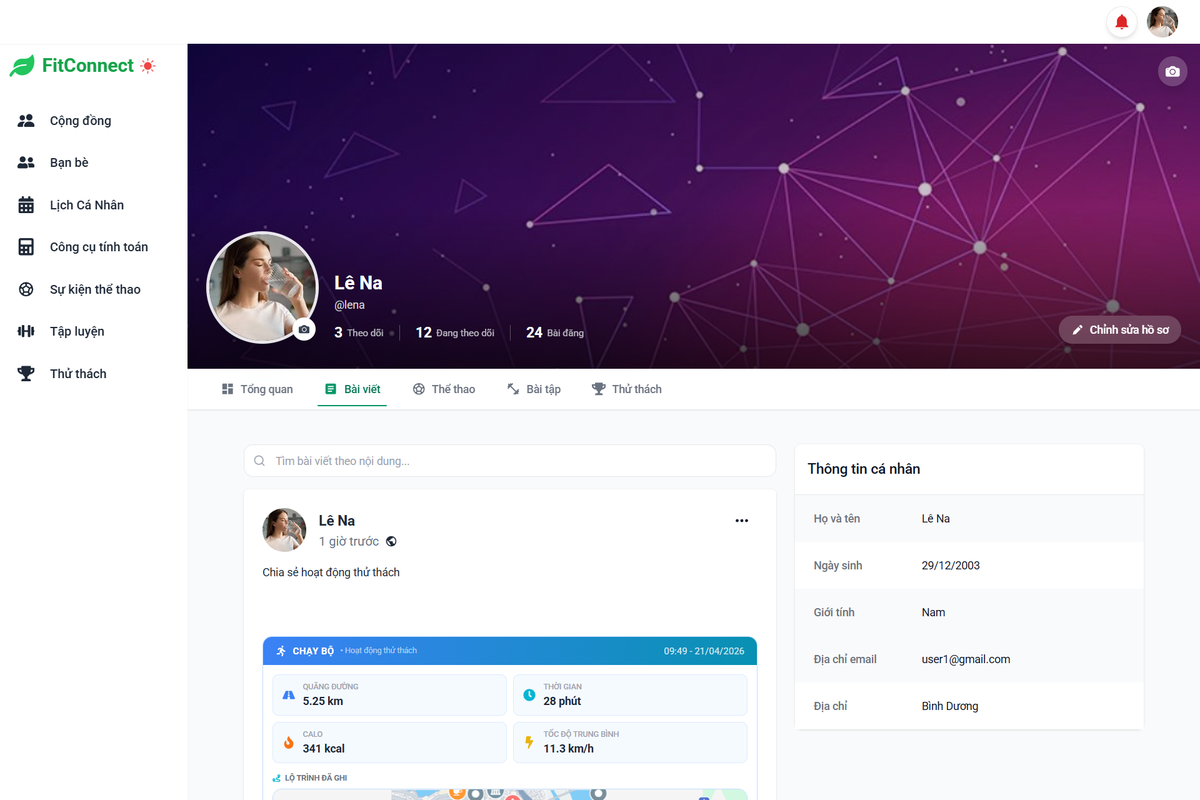
\includegraphics[width=\textwidth]{Images/IMG/Nhom1/tabtongquanbaiviet.png}
        \caption{Tab Bài viết}
        \label{fig:impl_profile_posts_tab}
    \end{subfigure}
    \hfill
    \begin{subfigure}[b]{0.30\textwidth}
        \centering
        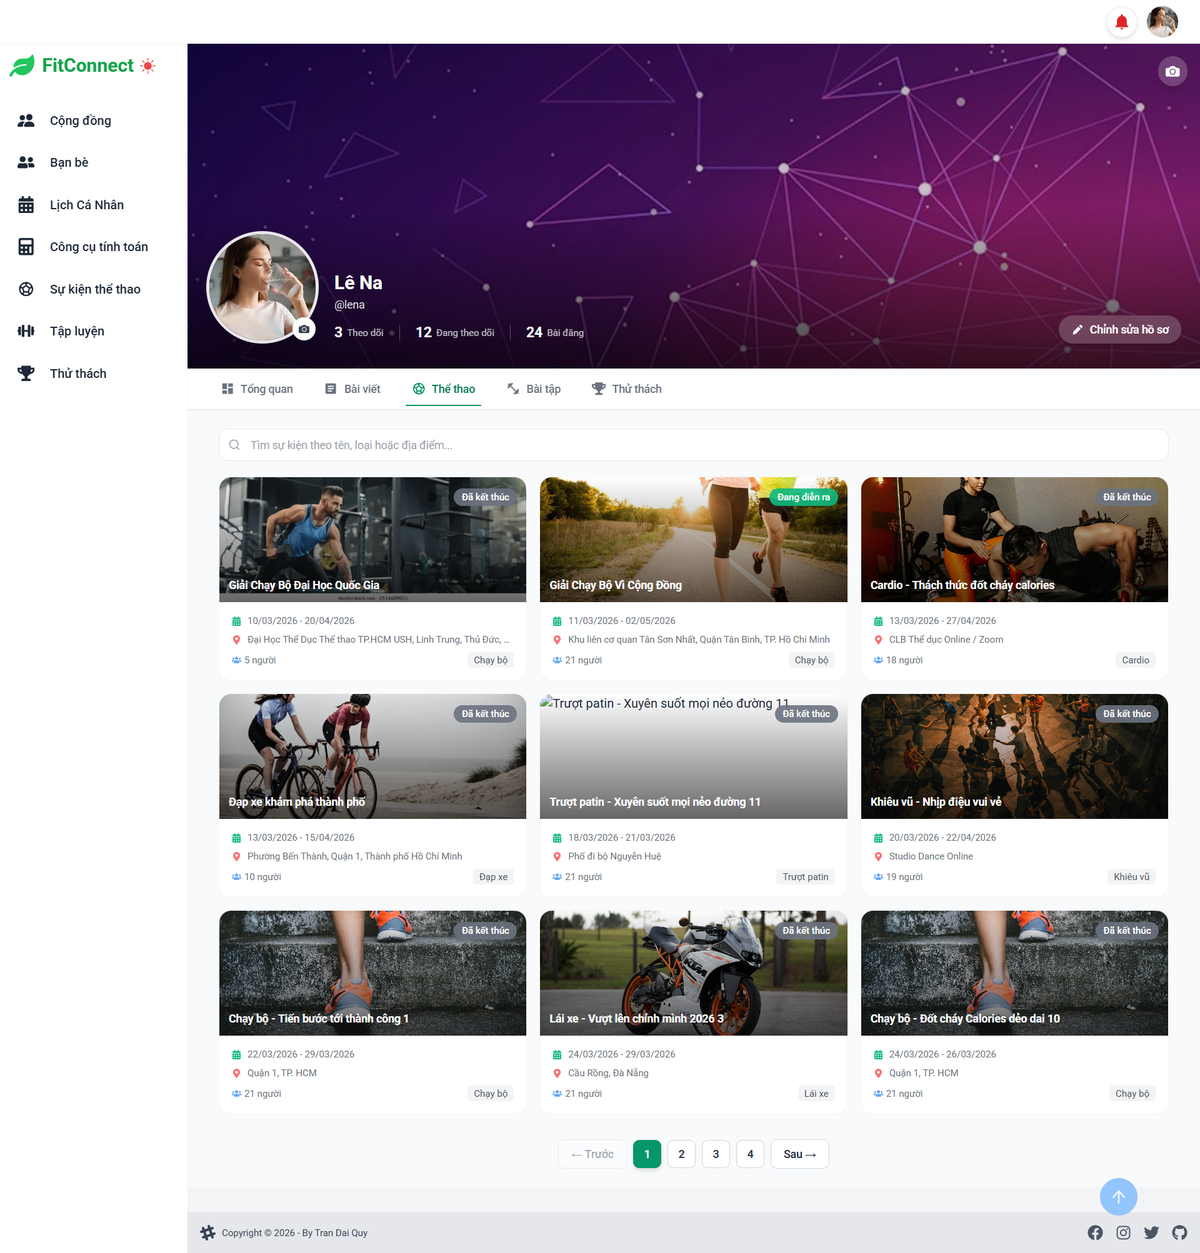
\includegraphics[width=\textwidth]{Images/IMG/Nhom1/tabsukien.png}
        \caption{Tab Sự kiện}
        \label{fig:impl_profile_events_tab}
    \end{subfigure}
    \hfill
    \begin{subfigure}[b]{0.30\textwidth}
        \centering
        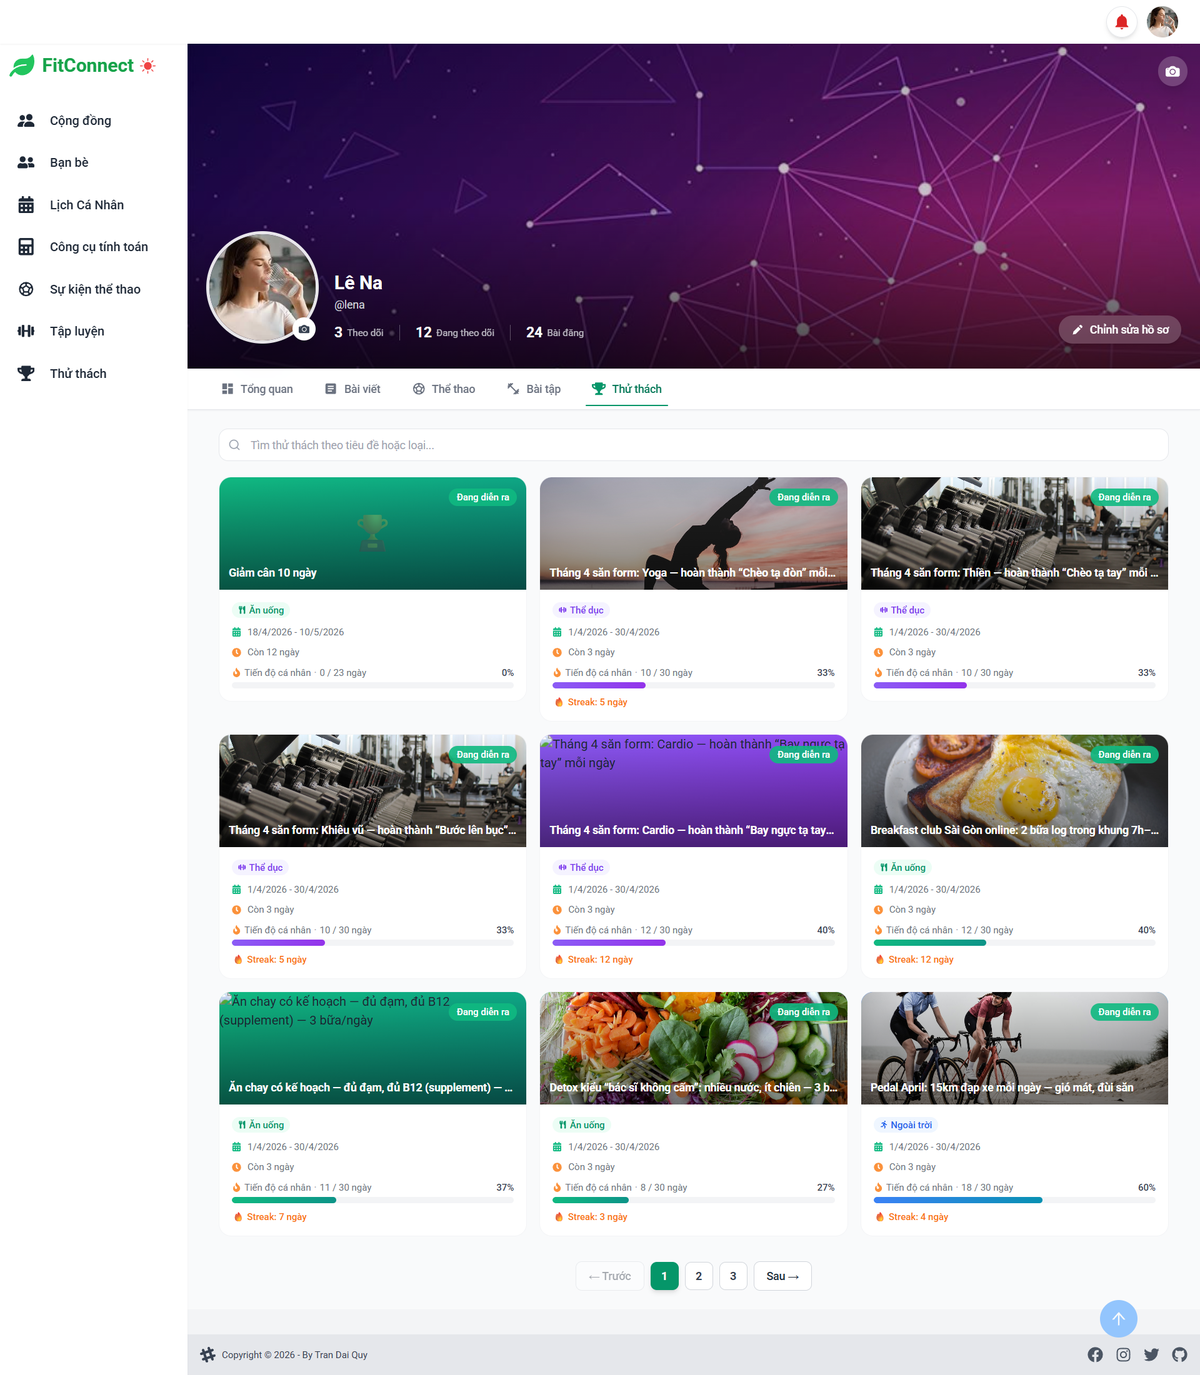
\includegraphics[width=\textwidth]{Images/IMG/Nhom1/tabthuthach.png}
        \caption{Tab Thử thách}
        \label{fig:impl_profile_challenges_tab}
    \end{subfigure}
    \vspace{0.3em}
    \caption{Ba tab theo dõi hoạt động trên trang cá nhân Profile Dashboard}
    \label{fig:impl_profile_tabs}
\end{figure}


    \item Để cá nhân hóa giao diện hồ sơ, người dùng có thể thay đổi ảnh đại diện và ảnh nền thông qua các modal thao tác nhanh. Cơ chế này cho phép cập nhật trực tiếp trên trang cá nhân mà không cần chuyển trang.

\begin{figure}[H]
    \centering
    \begin{subfigure}[b]{0.47\textwidth}
        \centering
        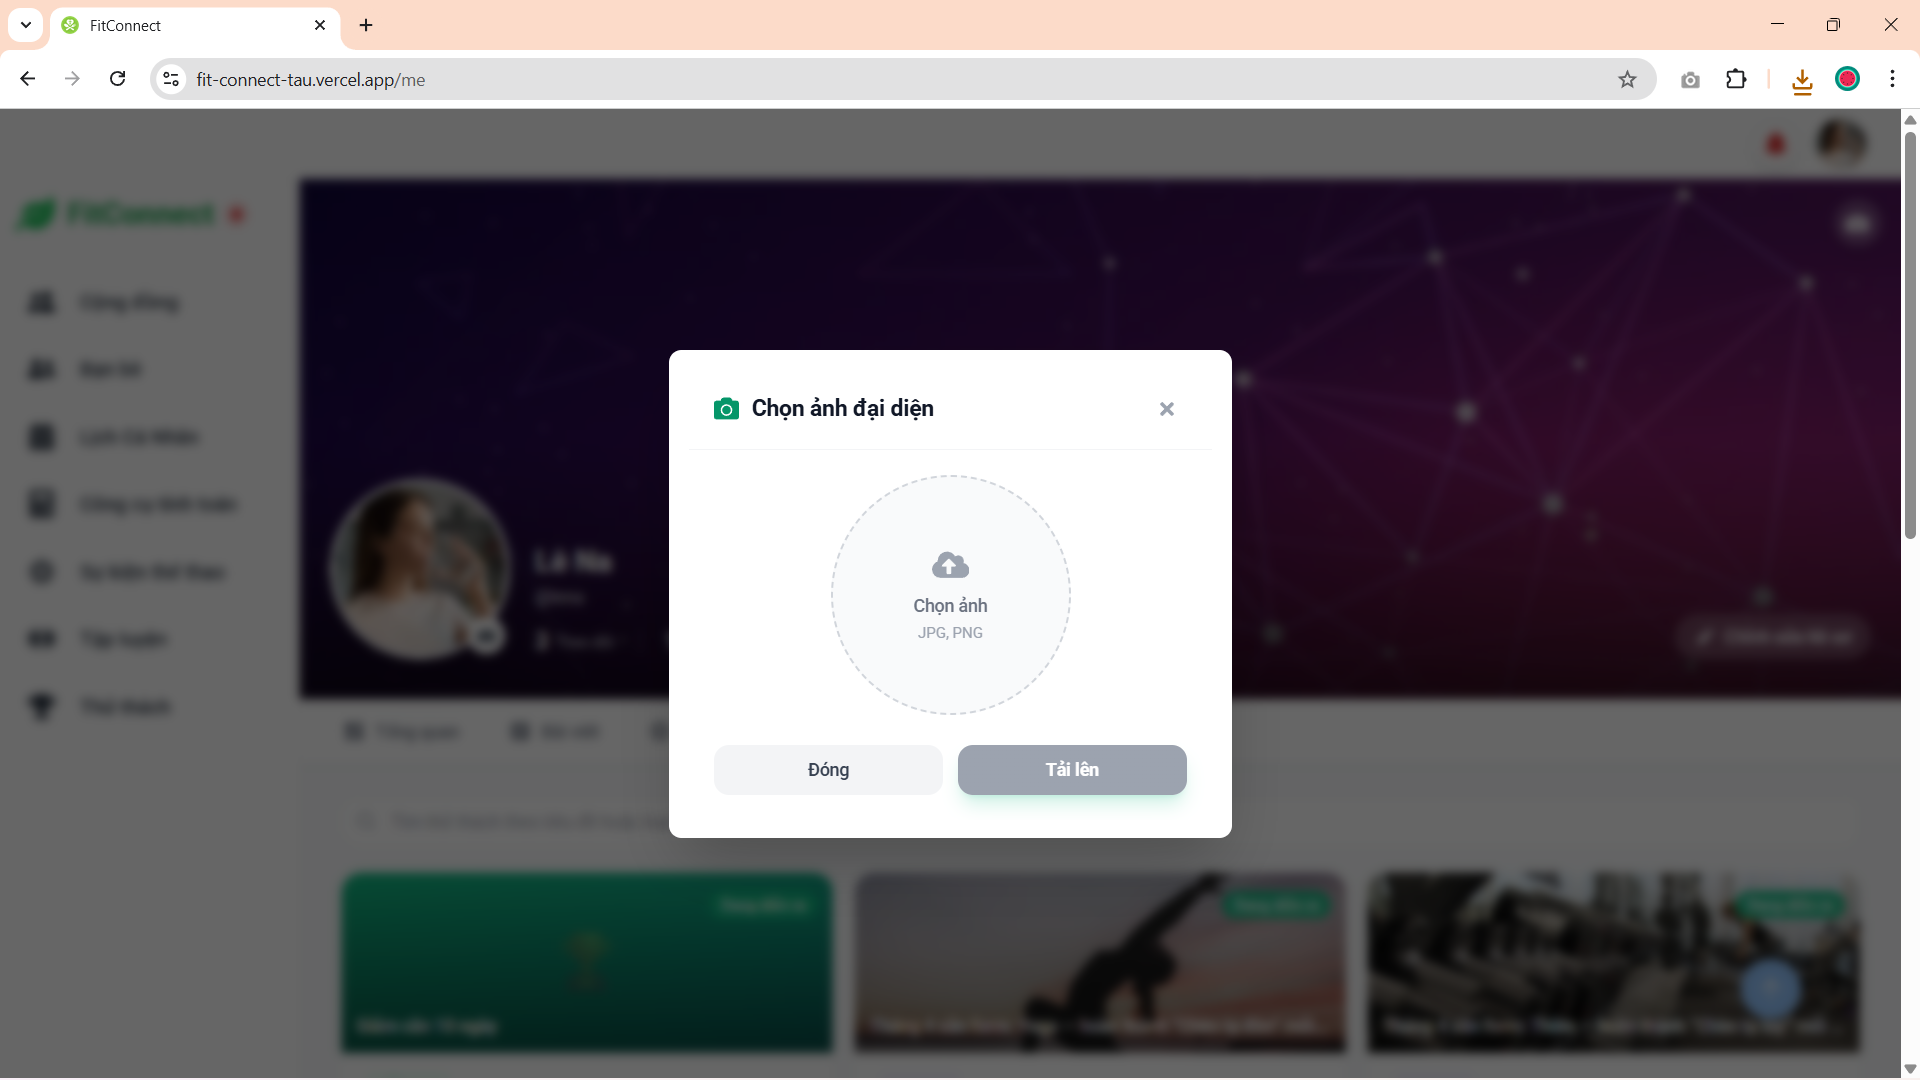
\includegraphics[width=\textwidth]{Images/IMG/Nhom1/modaldoiavatar.png}
        \caption{Modal thay đổi ảnh đại diện trên trang cá nhân}
        \label{fig:impl_profile_avatar_modal}
    \end{subfigure}
    \hfill
    \begin{subfigure}[b]{0.47\textwidth}
        \centering
        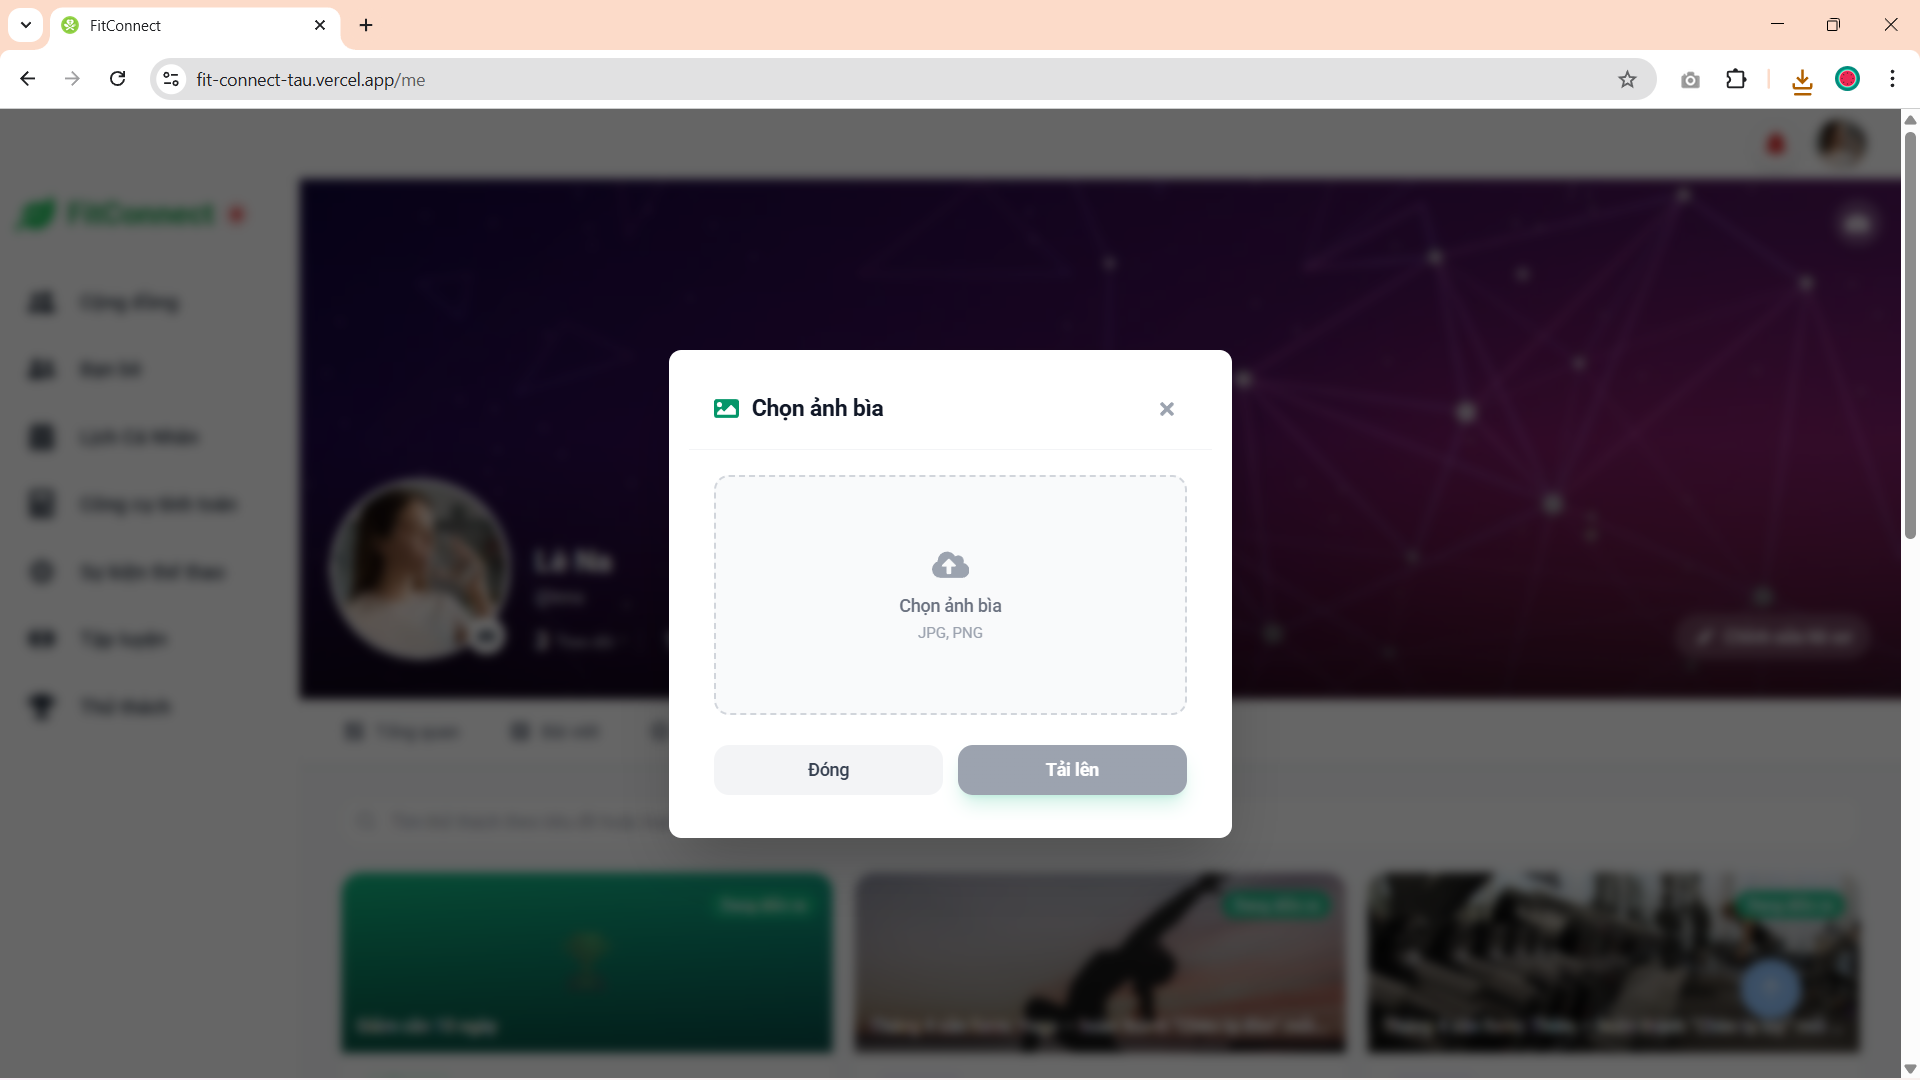
\includegraphics[width=\textwidth]{Images/IMG/Nhom1/modaldoibackgroud.png}
        \caption{Modal thay đổi ảnh nền trang cá nhân}
        \label{fig:impl_profile_cover_modal}
    \end{subfigure}
\end{figure}


    \item Ngoài phần hiển thị, người dùng có thể cập nhật thông tin hồ sơ (thông tin cá nhân và nhân trắc học) và thay đổi mật khẩu để tăng cường quản trị tài khoản, bảo đảm tính chính xác dữ liệu và an toàn truy cập.

\begin{figure}[H]
    \centering
    \begin{subfigure}[b]{0.47\textwidth}
        \centering
        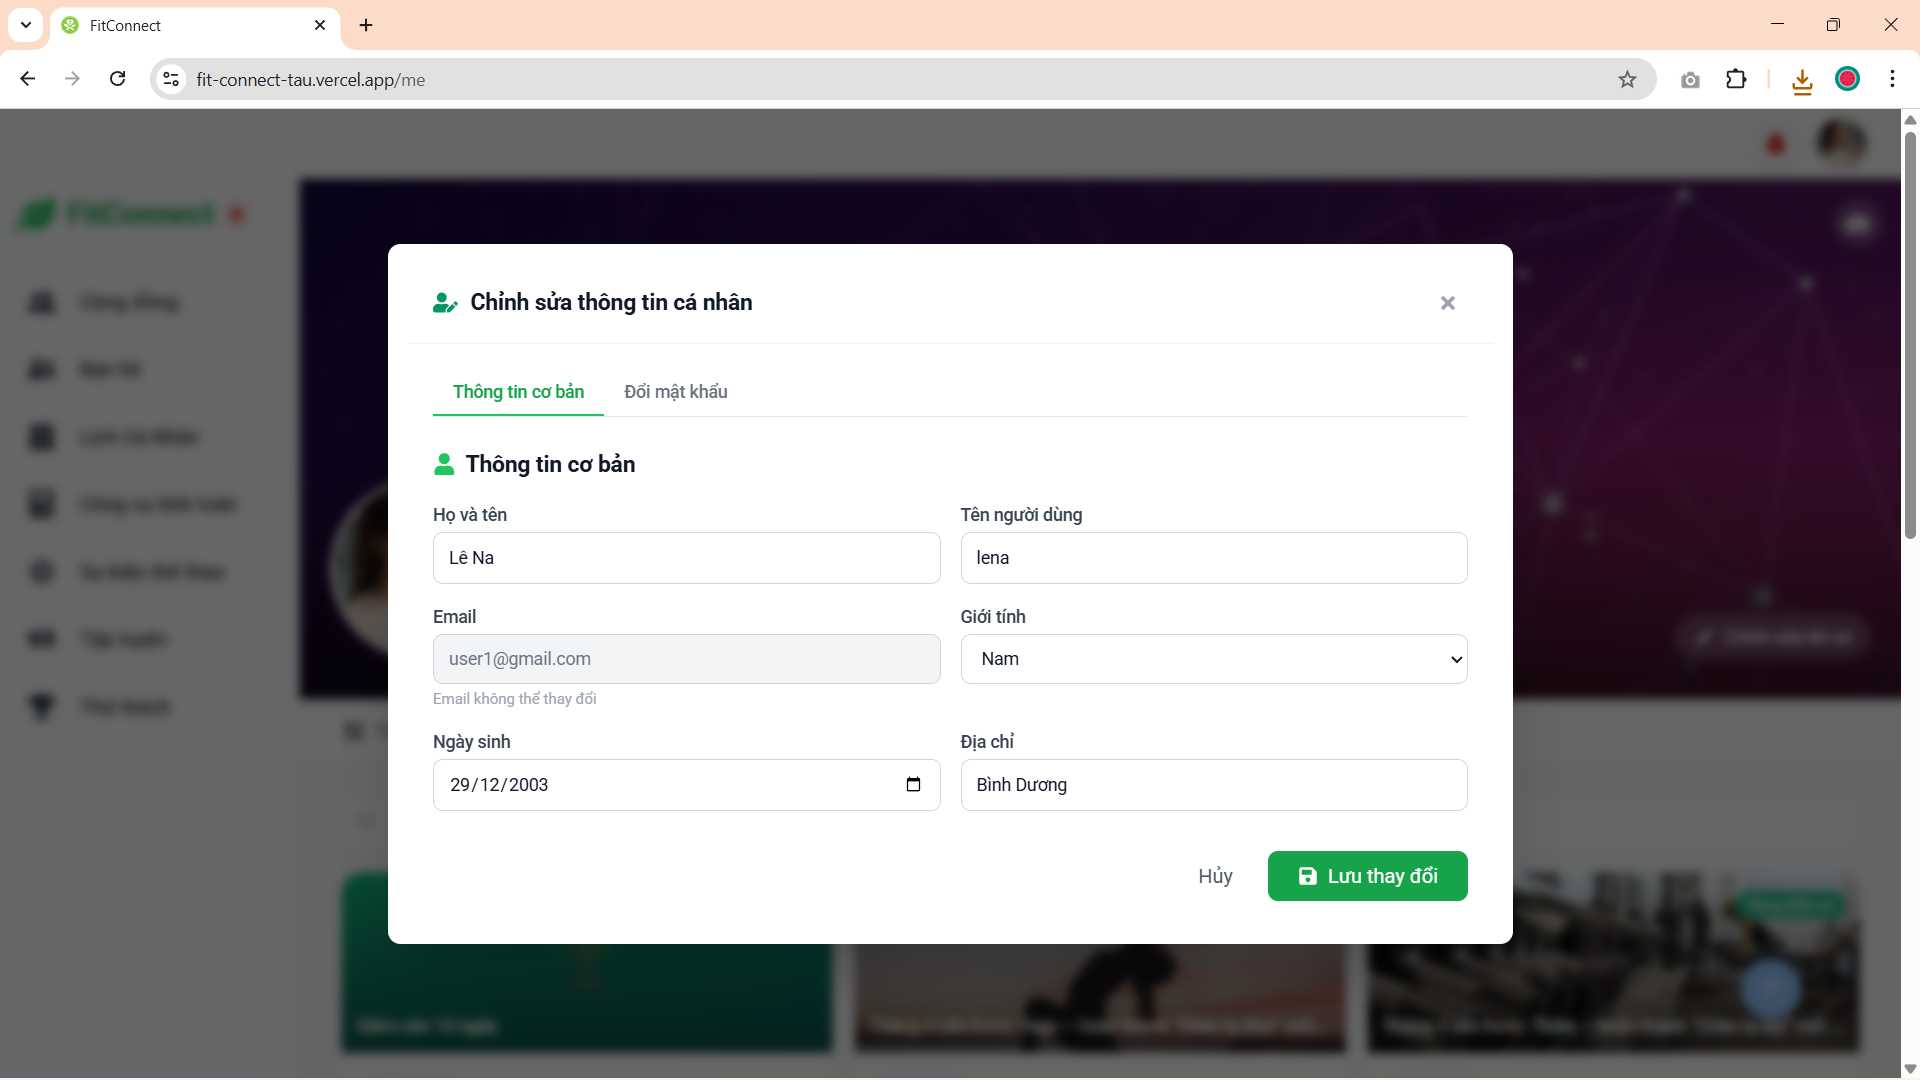
\includegraphics[width=\textwidth]{Images/IMG/Nhom1/capnhatthongtin.png}
        \caption{Người dùng cập nhật thông tin hồ sơ cá nhân}
        \label{fig:impl_profile_update}
    \end{subfigure}
    \hfill
    \begin{subfigure}[b]{0.47\textwidth}
        \centering
        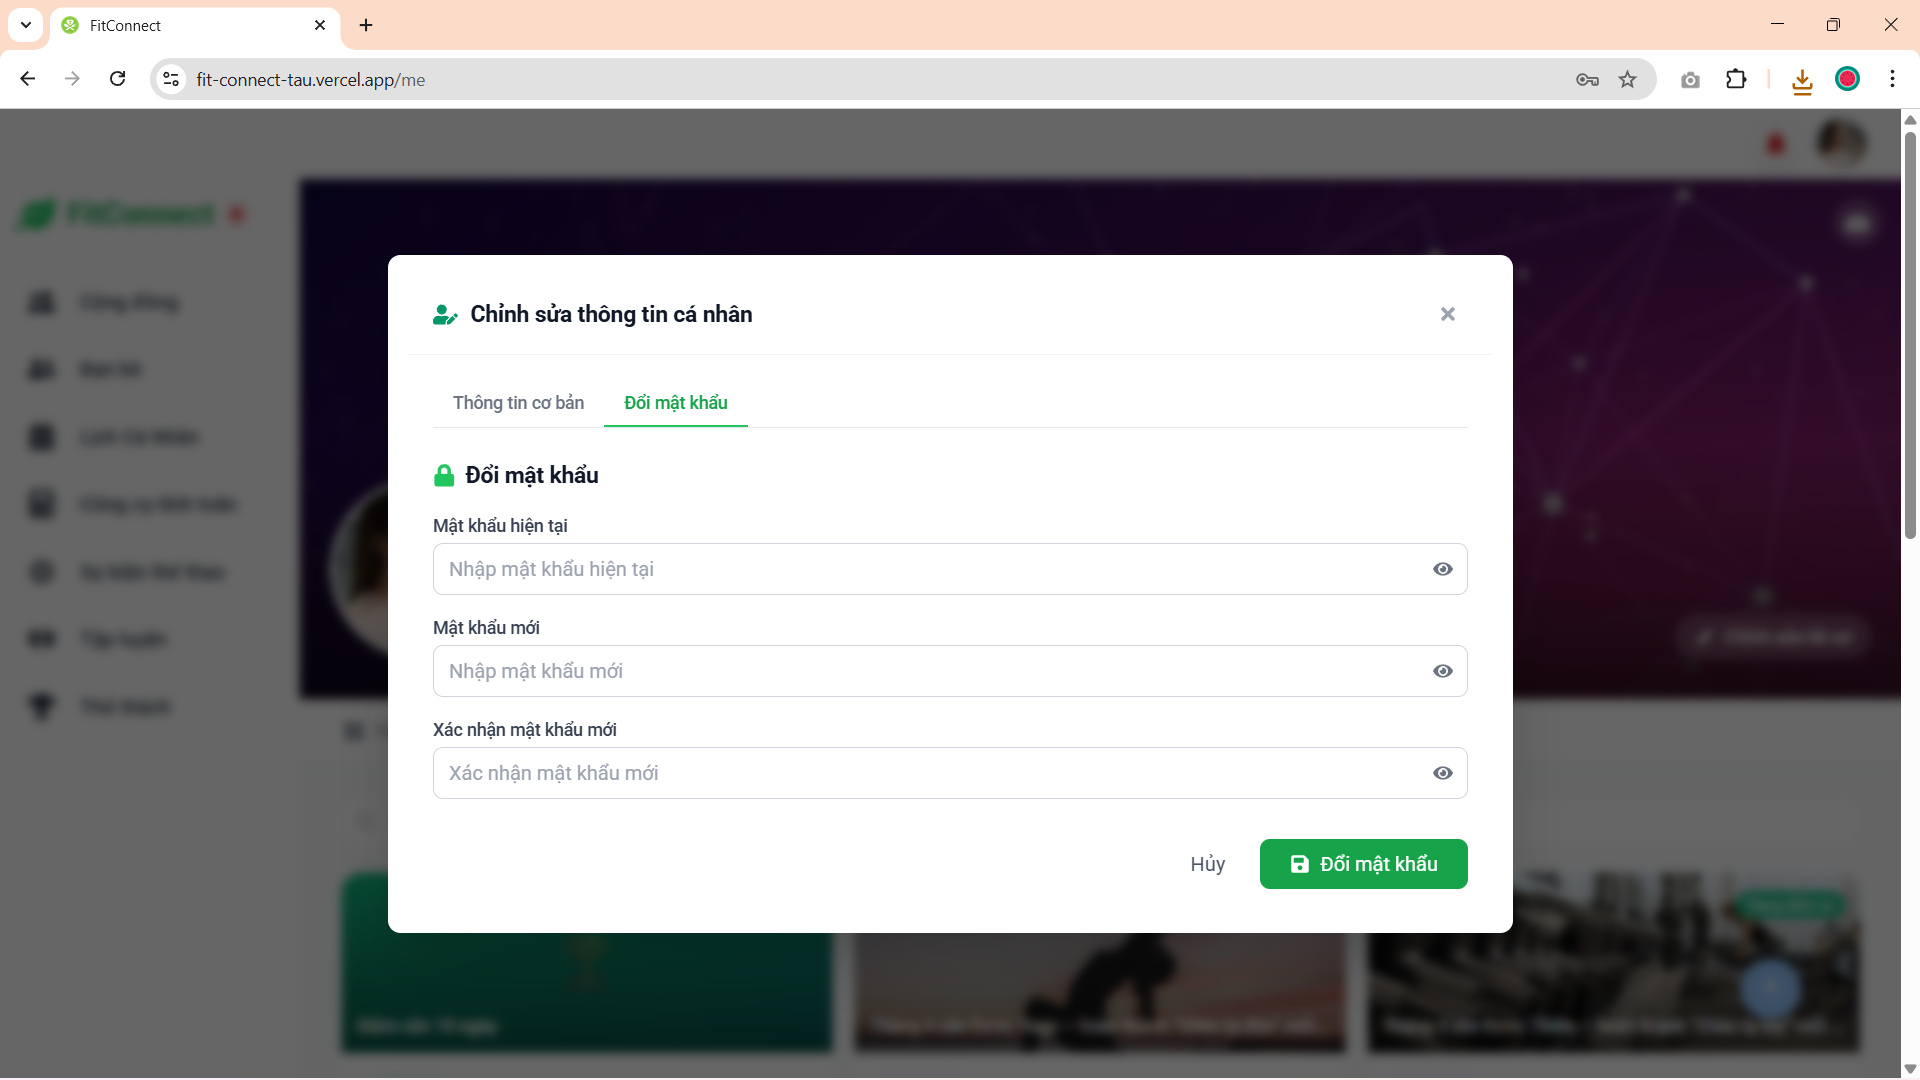
\includegraphics[width=\textwidth]{Images/IMG/Nhom1/capnhatmatkhau.png}
        \caption{Người dùng cập nhật mật khẩu trong khu vực quản trị hồ sơ}
        \label{fig:impl_profile_change_password}
    \end{subfigure}
\end{figure}

\end{itemize}


\subsection{Nhóm tính năng Mạng xã hội cộng đồng}
\label{subsec:impl_social}

Nhóm tính năng Mạng xã hội cộng đồng đóng vai trò là cầu nối gắn kết mọi người lại với nhau, giúp họ dễ dàng kết nối, chia sẻ và tương tác với nhau thông qua những bài viết, sự kiện thể thao hay thử thách cộng đồng được chia sẻ. Đây là nơi mọi người có thể đăng tải, chia sẻ bài viết, hình ảnh, sự kiện, thử thách,... mình yêu thích cũng như theo dõi và tương tác với những người có cùng sở thích.

Sự khác biệt của hệ thống nằm ở việc mạng xã hội cộng đồng này không chỉ dừng lại ở việc cung cấp diễn đàn mạng xã hội như các nền tảng truyền thống, mà còn là một hệ sinh thái tích hợp đầy đủ và toàn diện tính năng của mạng xã hội kết hợp với tính năng quản trị nội dung bài viết giúp mọi nội dung bài viết mà mọi người tiếp cận luôn trong sạch, lành mạnh và giúp kịp thời phát hiện xử lý những nội dung không lành mạnh với sự chung tay từ phía người dùng và quản trị viên.

Quy trình hoạt động gồm hai luồng chính:
\begin{itemize}
    \item \textbf{Người dùng:} Cho phép đăng, tương tác bài viết, báo cáo bài viết tới quản trị viên.
    \item \textbf{Quản trị viên:} Xử lý các bài viết bị báo cáo từ người dùng.
\end{itemize}

\subsubsection{Luồng thao tác Bảng tin (Góc độ Người dùng)}
\begin{itemize}
    \item Người dùng xem bảng tin bài viết Cộng đồng: Khi nhấn vào mục Cộng đồng, người dùng sẽ có thể xem được những bài viết từ cộng đồng. Hệ thống sẽ luôn cập nhật thời gian thực để giúp luôn hiển thị các bài viết mới nhất trên newfeeds của người dùng.

\begin{figure}[H]
    \centering
    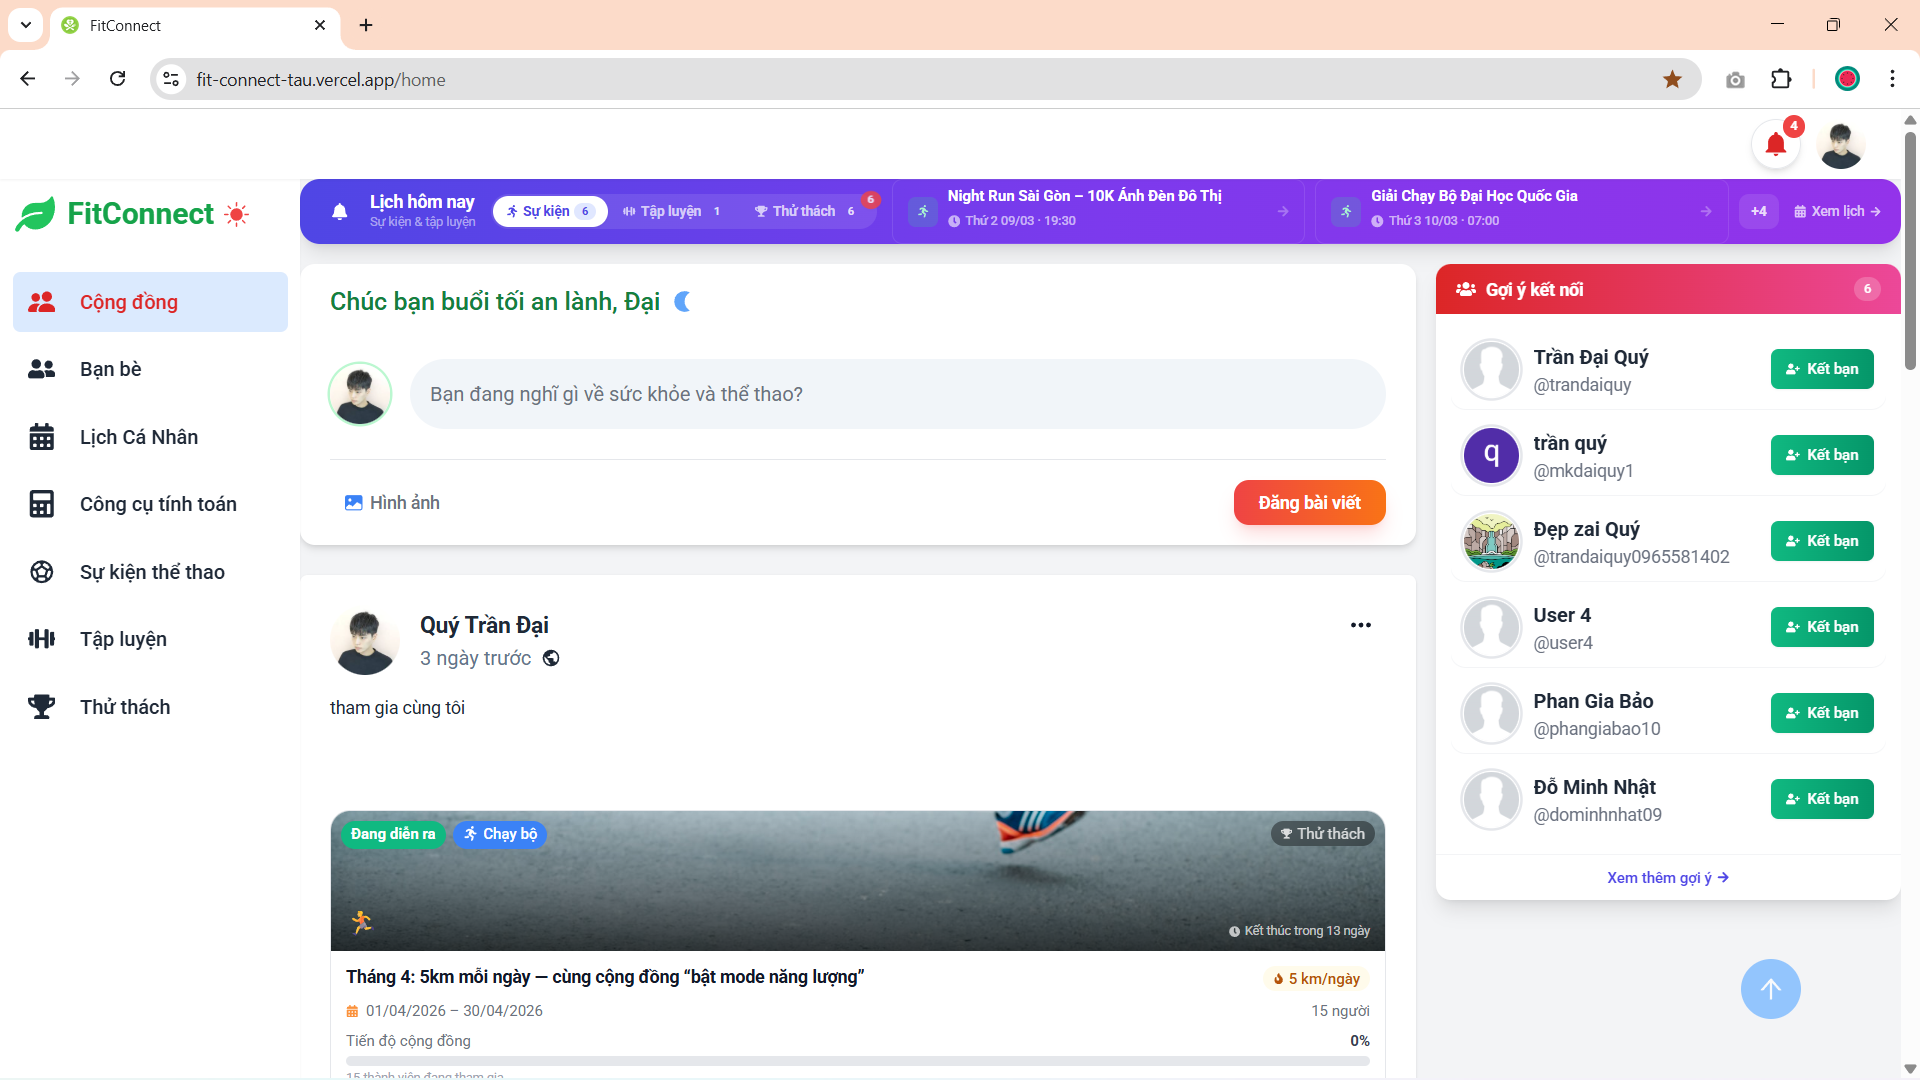
\includegraphics[width=0.60\textwidth]{Images/IMG/Nhom2/trangchucongdong.png}
    \caption{Người dùng xem trang chủ cộng đồng}
    \label{fig:impl_social_home}
\end{figure}


    \item Người dùng tạo bài viết mới: hệ thống hiển thị Modal soạn nội dung, chèn hình ảnh (tối đa 5 ảnh), đính kèm biểu tượng cảm xúc và chọn đối tượng hướng đến. Khi nhấn Đăng, AI tự động kiểm tra hình ảnh: nếu phát hiện nội dung nhạy cảm, bài viết bị chặn với cảnh báo; nếu hợp lệ, bài viết được đăng và bảng tin tự động làm mới.

\begin{figure}[H]
    \centering
    \begin{subfigure}[b]{0.47\textwidth}
        \centering
        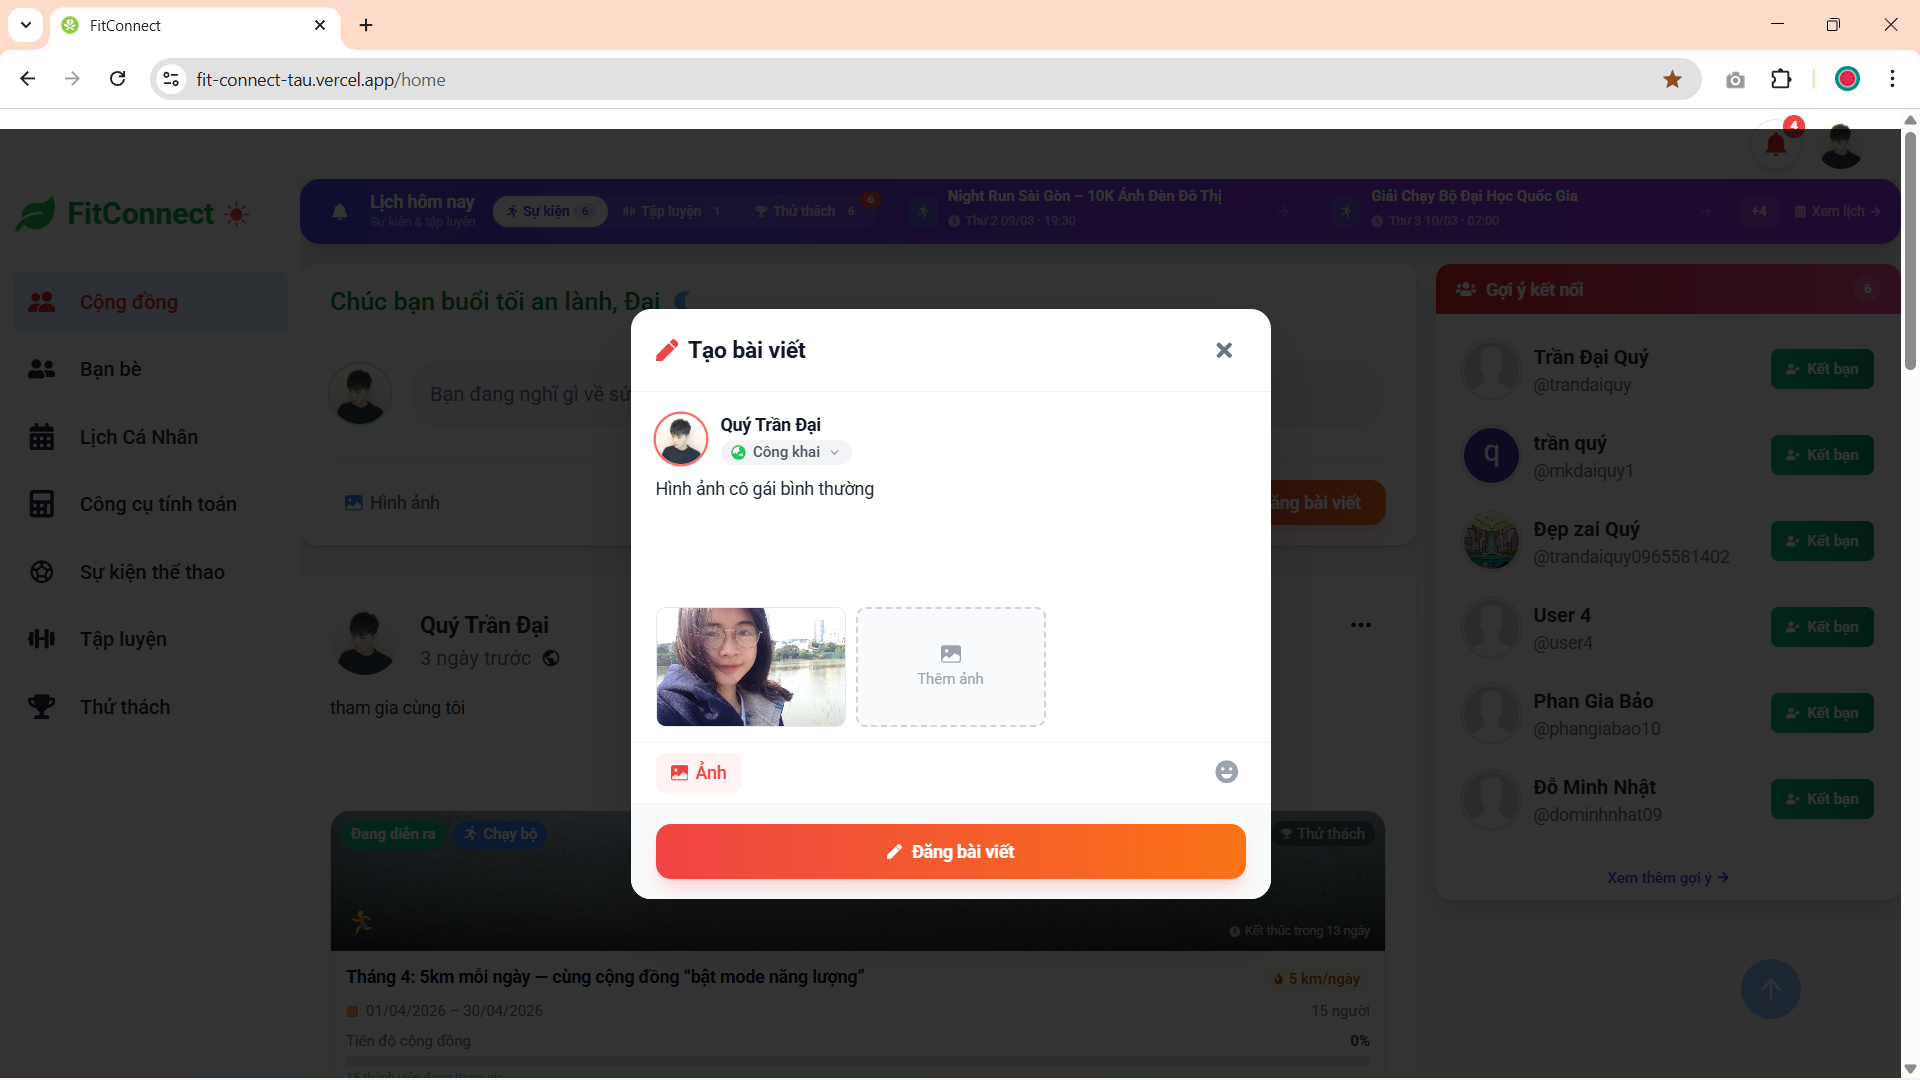
\includegraphics[width=\textwidth]{Images/IMG/Nhom2/dangbaivietbinhthuong.png}
        \caption{Modal soạn và đăng bài viết bình thường}
        \label{fig:impl_social_post}
    \end{subfigure}
    \hfill
    \begin{subfigure}[b]{0.47\textwidth}
        \centering
        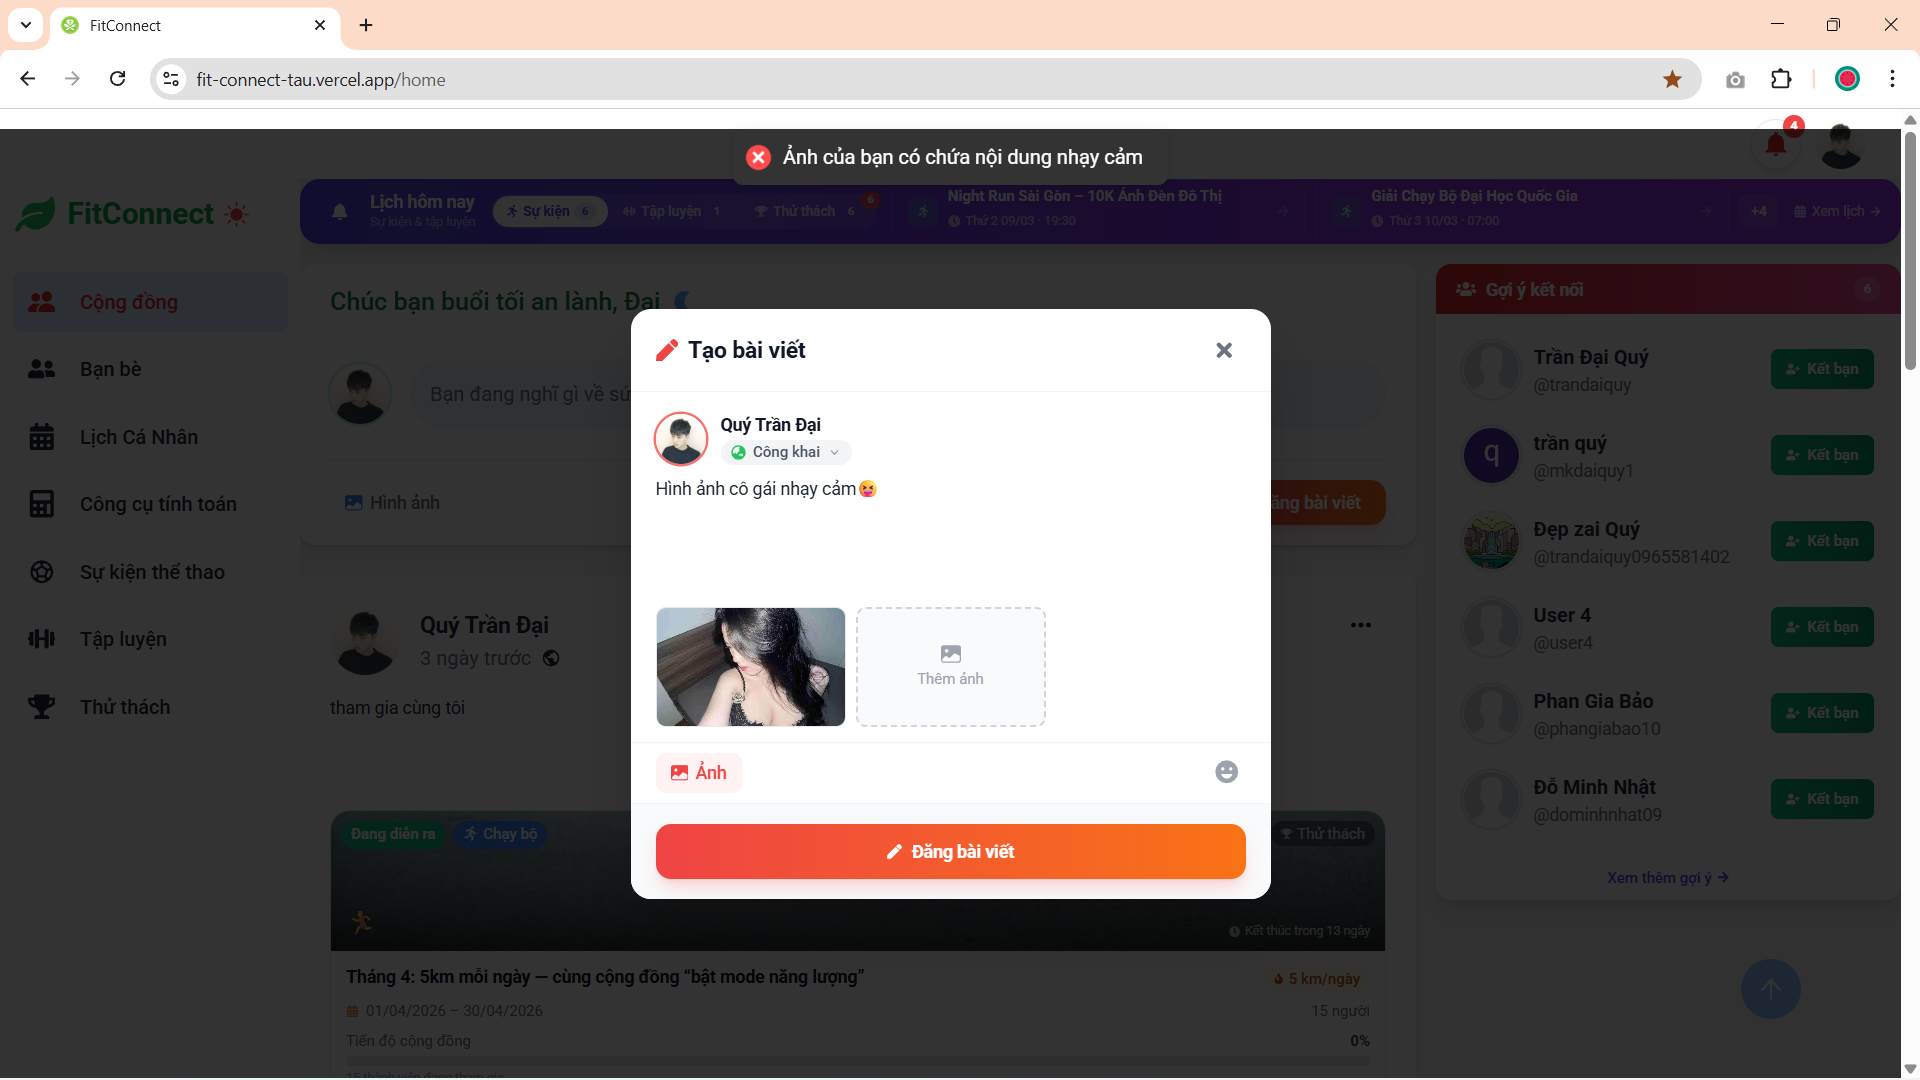
\includegraphics[width=\textwidth]{Images/IMG/Nhom2/dangbaivietchuahinhanhvipham.png}
        \caption{Hệ thống chặn đăng bài khi phát hiện hình ảnh vi phạm}
        \label{fig:impl_social_violate}
    \end{subfigure}
    \vspace{0.3em}
    \caption{Luồng đăng bài viết với kiểm duyệt AI hình ảnh tự động}
    \label{fig:impl_social_post_flow}
\end{figure}

    \item Những người dùng khác trong hệ thống có thể tương tác thích và bình luận về bài viết. Người dùng có thể trả lời những bình luận của nhau, giúp trao đổi tương tác liên tục.

\begin{figure}[H]
    \centering
    \begin{subfigure}[b]{0.47\textwidth}
        \centering
        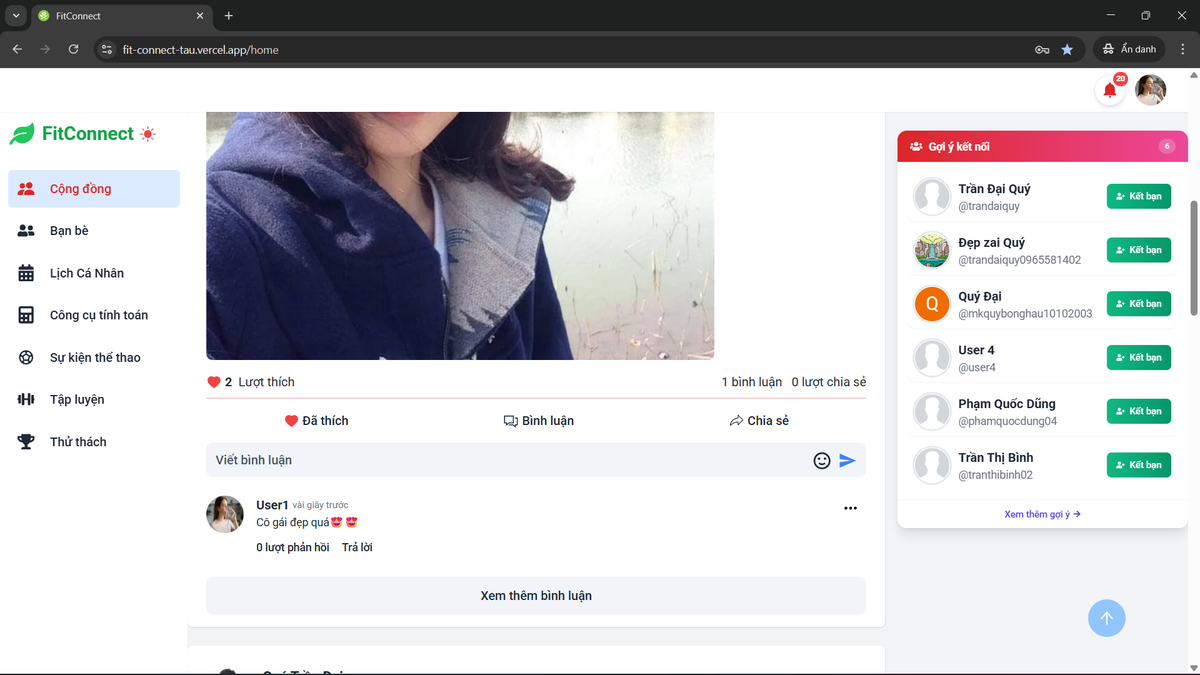
\includegraphics[width=\textwidth]{Images/IMG/Nhom2/nguoikhacthichvabinhluan.png}
        \caption{Người dùng nhận thông báo khi người khác thích và bình luận}
        \label{fig:impl_social_interact}
    \end{subfigure}
    \hfill
    \begin{subfigure}[b]{0.47\textwidth}
        \centering
        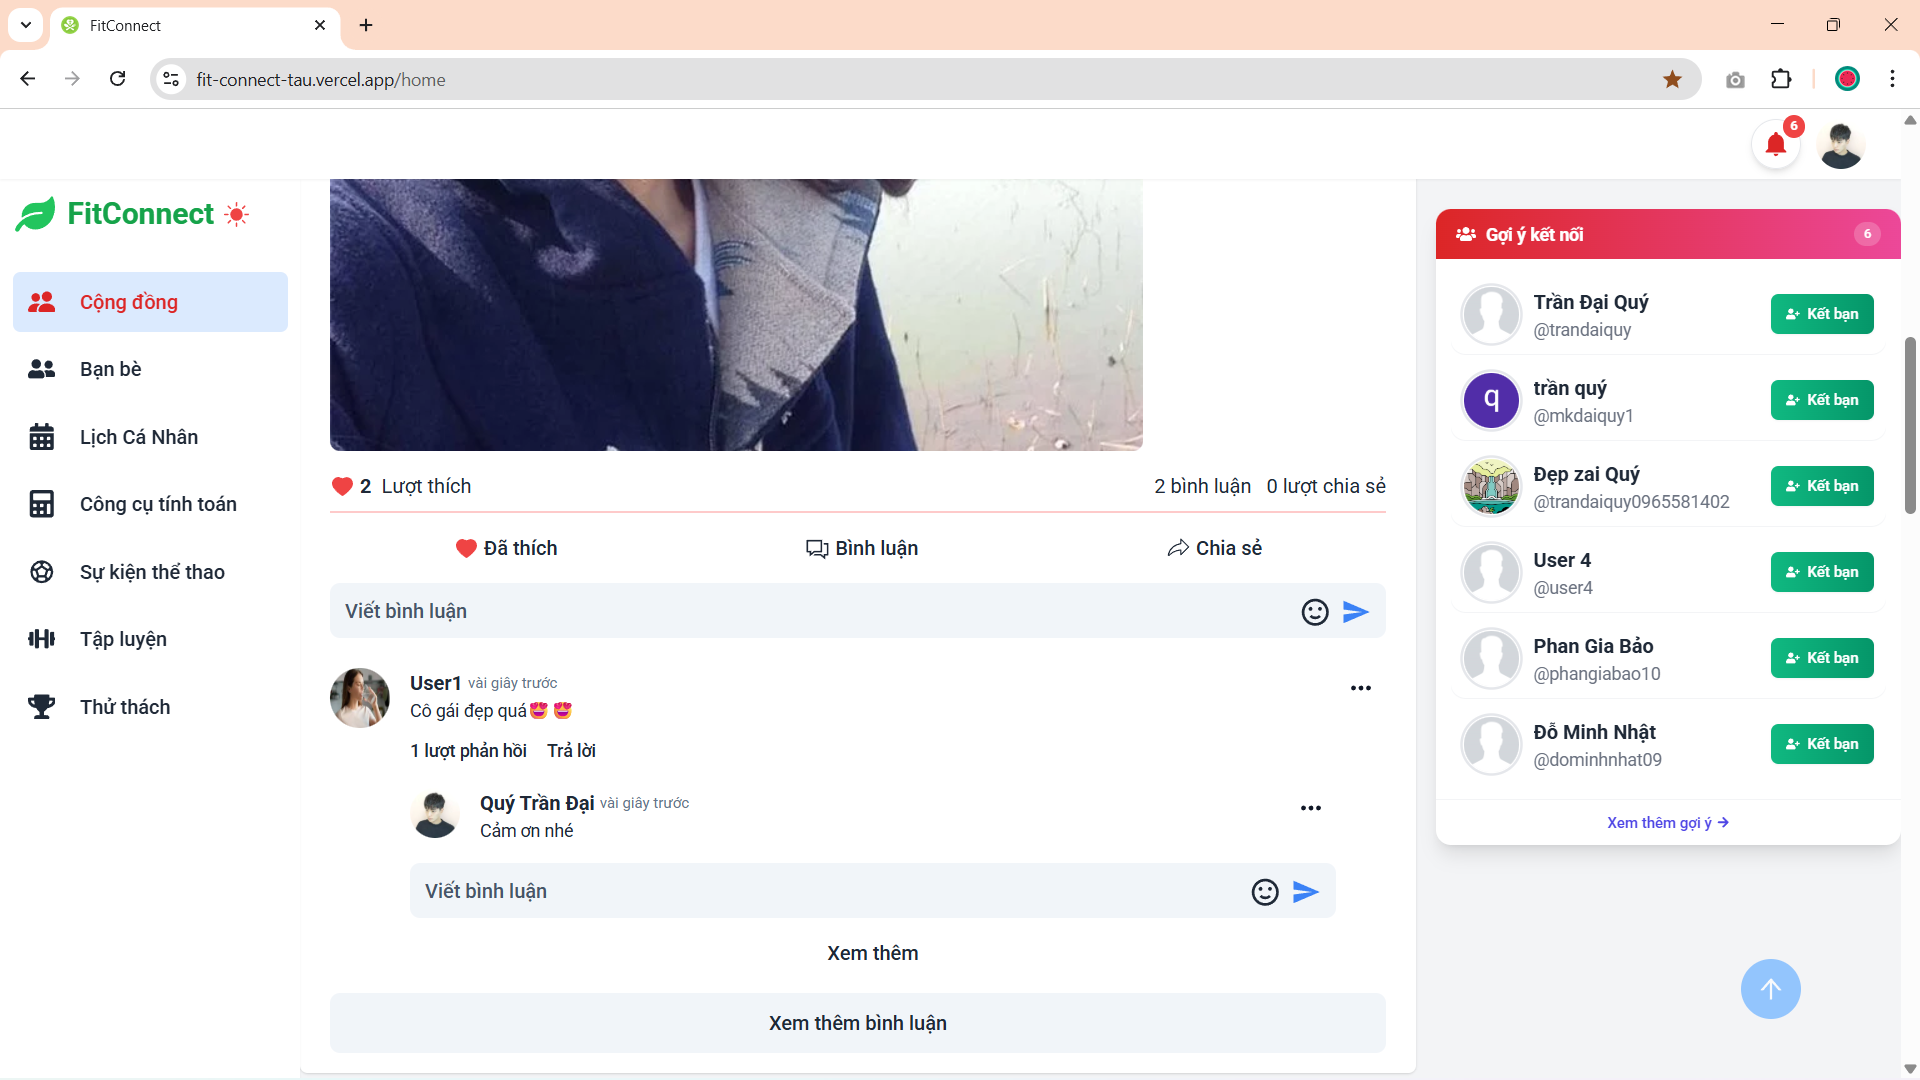
\includegraphics[width=\textwidth]{Images/IMG/Nhom2/traloibinhluannguoido.png}
        \caption{Người dùng thao tác trả lời bình luận người đó}
        \label{fig:impl_social_reply}
    \end{subfigure}
\end{figure}


    \item Người dùng có thể chia sẻ bài viết của người khác về Bảng tin của mình hoặc tự xóa bài viết của mình khi không còn phù hợp.

\begin{figure}[H]
    \centering
    \begin{subfigure}[b]{0.47\textwidth}
        \centering
        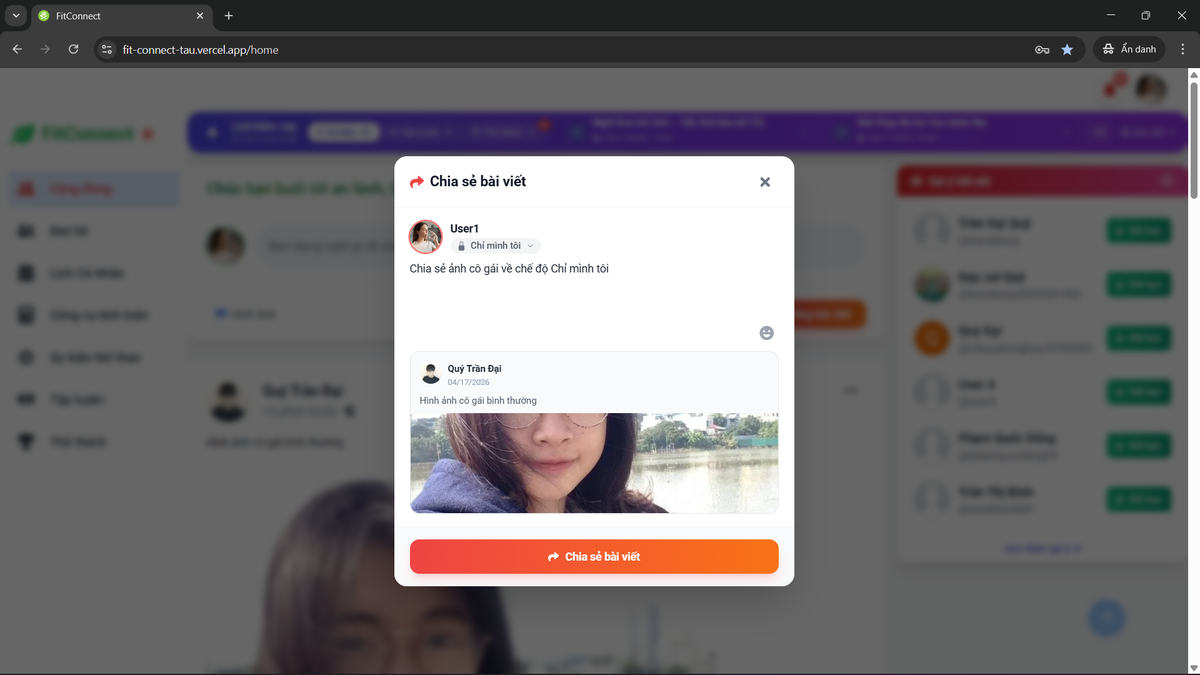
\includegraphics[width=\textwidth]{Images/IMG/Nhom2/chiasebaivietnguoikhac.png}
        \caption{Thao tác chia sẻ bài viết lên Bảng tin}
        \label{fig:impl_social_share}
    \end{subfigure}
    \hfill
    \begin{subfigure}[b]{0.47\textwidth}
        \centering
        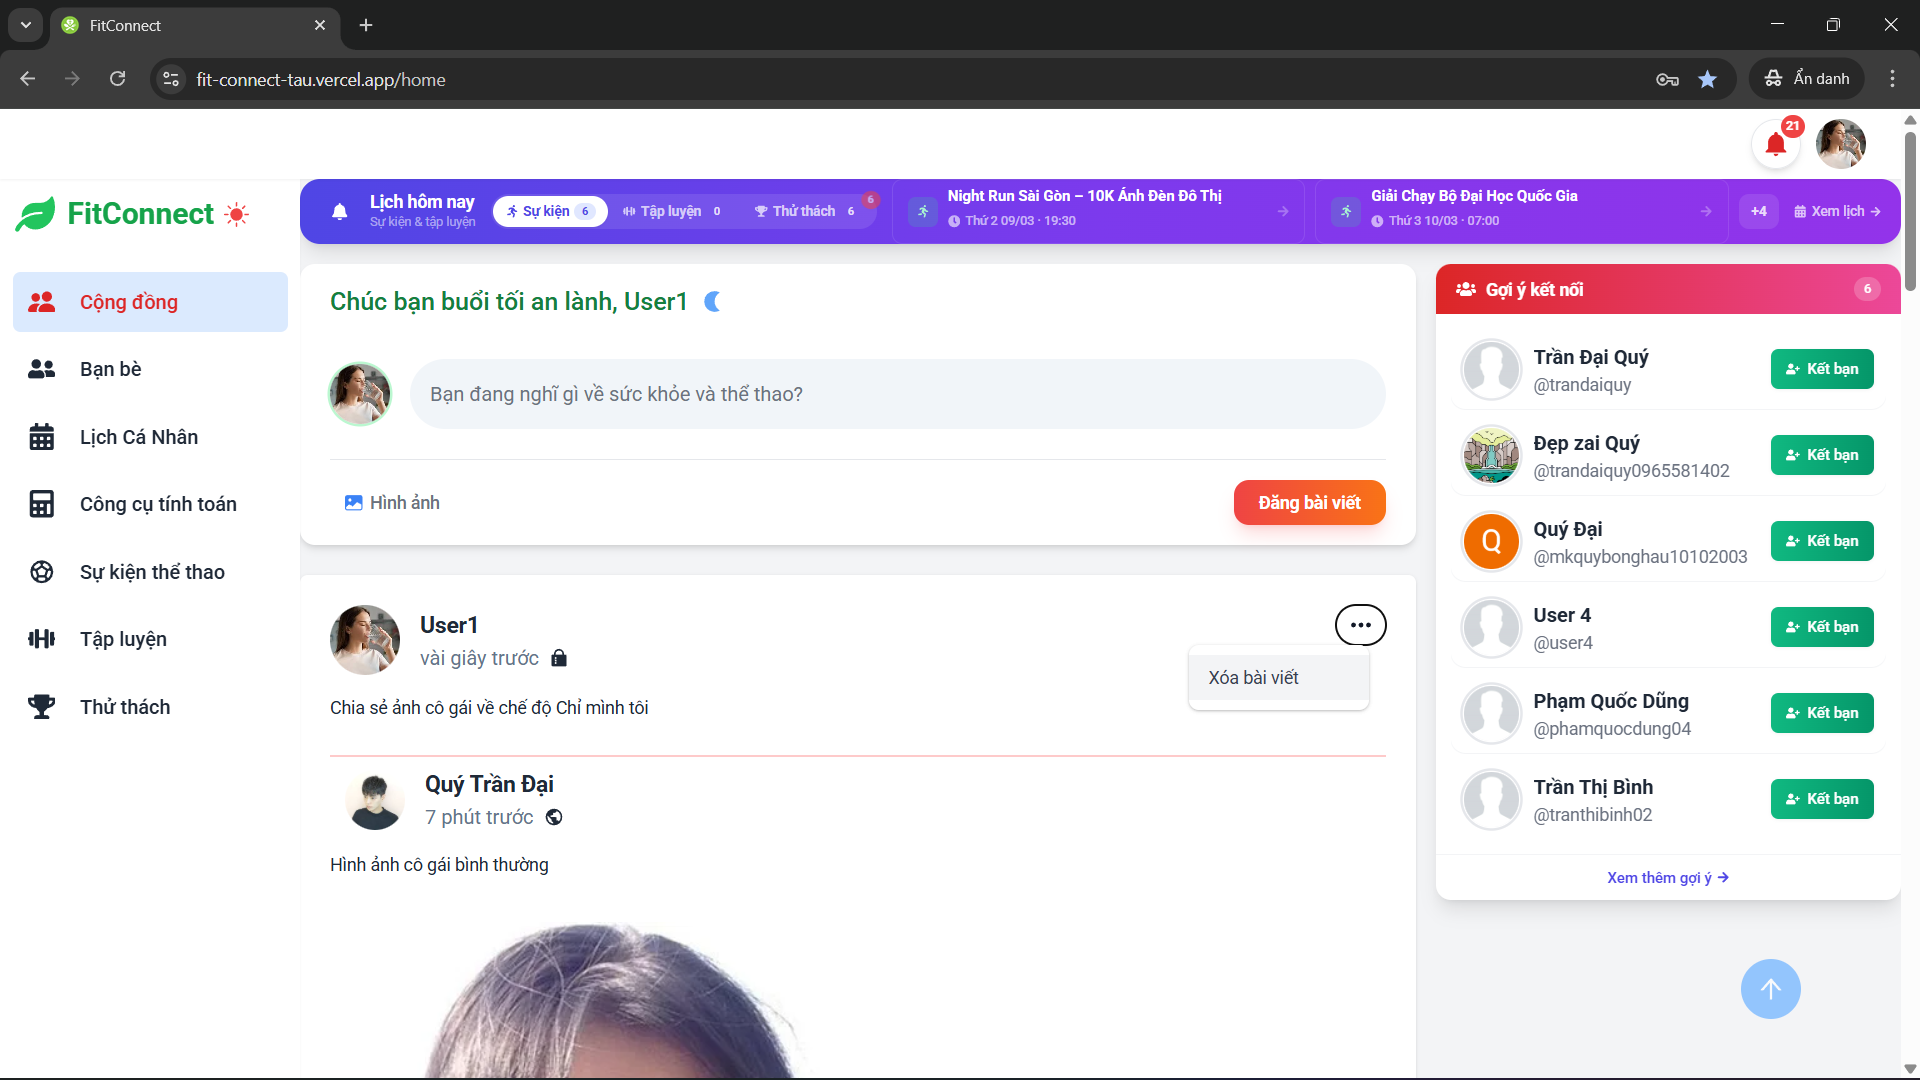
\includegraphics[width=\textwidth]{Images/IMG/Nhom2/xoabaiviet.png}
        \caption{Thao tác tự xóa bài viết của mình}
        \label{fig:impl_social_delete_own}
    \end{subfigure}
    \vspace{0.3em}
    \caption{Chia sẻ và xóa bài viết trên Bảng tin cộng đồng}
    \label{fig:impl_social_share_delete}
\end{figure}


    \item Người dùng có thể báo cáo những bài viết không hợp lệ lên quản trị viên. Khi đó người bị báo cáo sẽ nhận thông báo bài viết bị báo cáo.

\begin{figure}[H]
    \centering
    \begin{subfigure}[b]{0.47\textwidth}
        \centering
        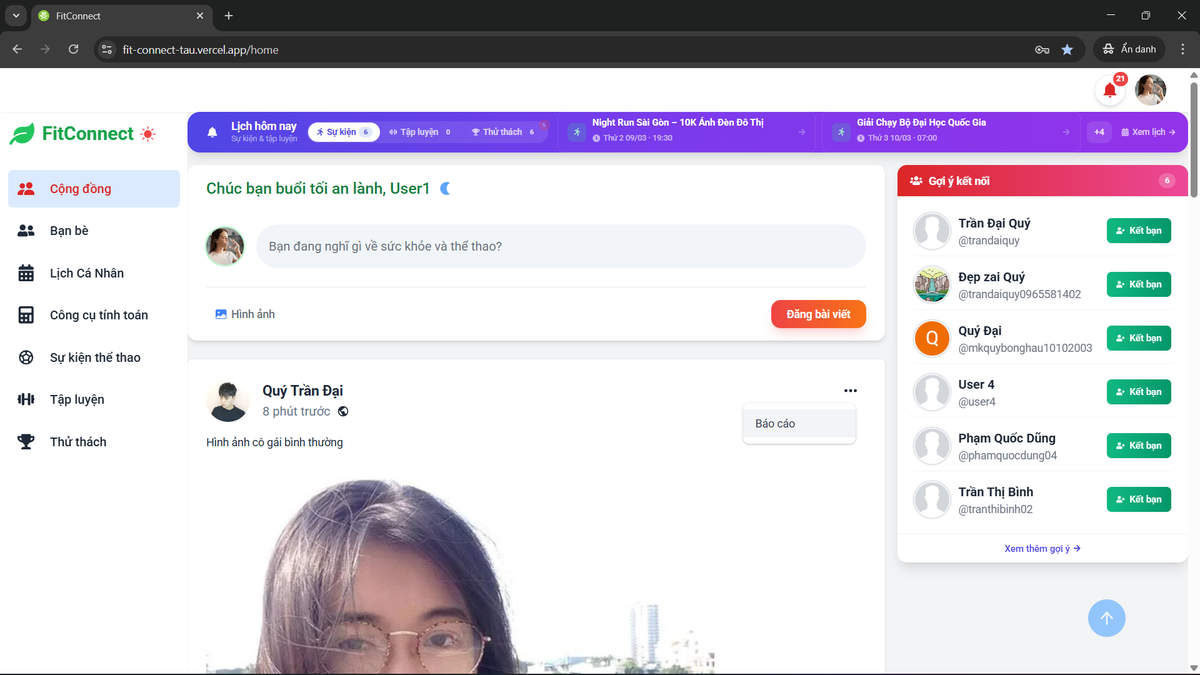
\includegraphics[width=\textwidth]{Images/IMG/Nhom2/baocaobaivietnguoikhac.png}
        \caption{Người dùng thao tác báo cáo bài viết người khác}
        \label{fig:impl_social_report}
    \end{subfigure}
    \hfill
    \begin{subfigure}[b]{0.47\textwidth}
        \centering
        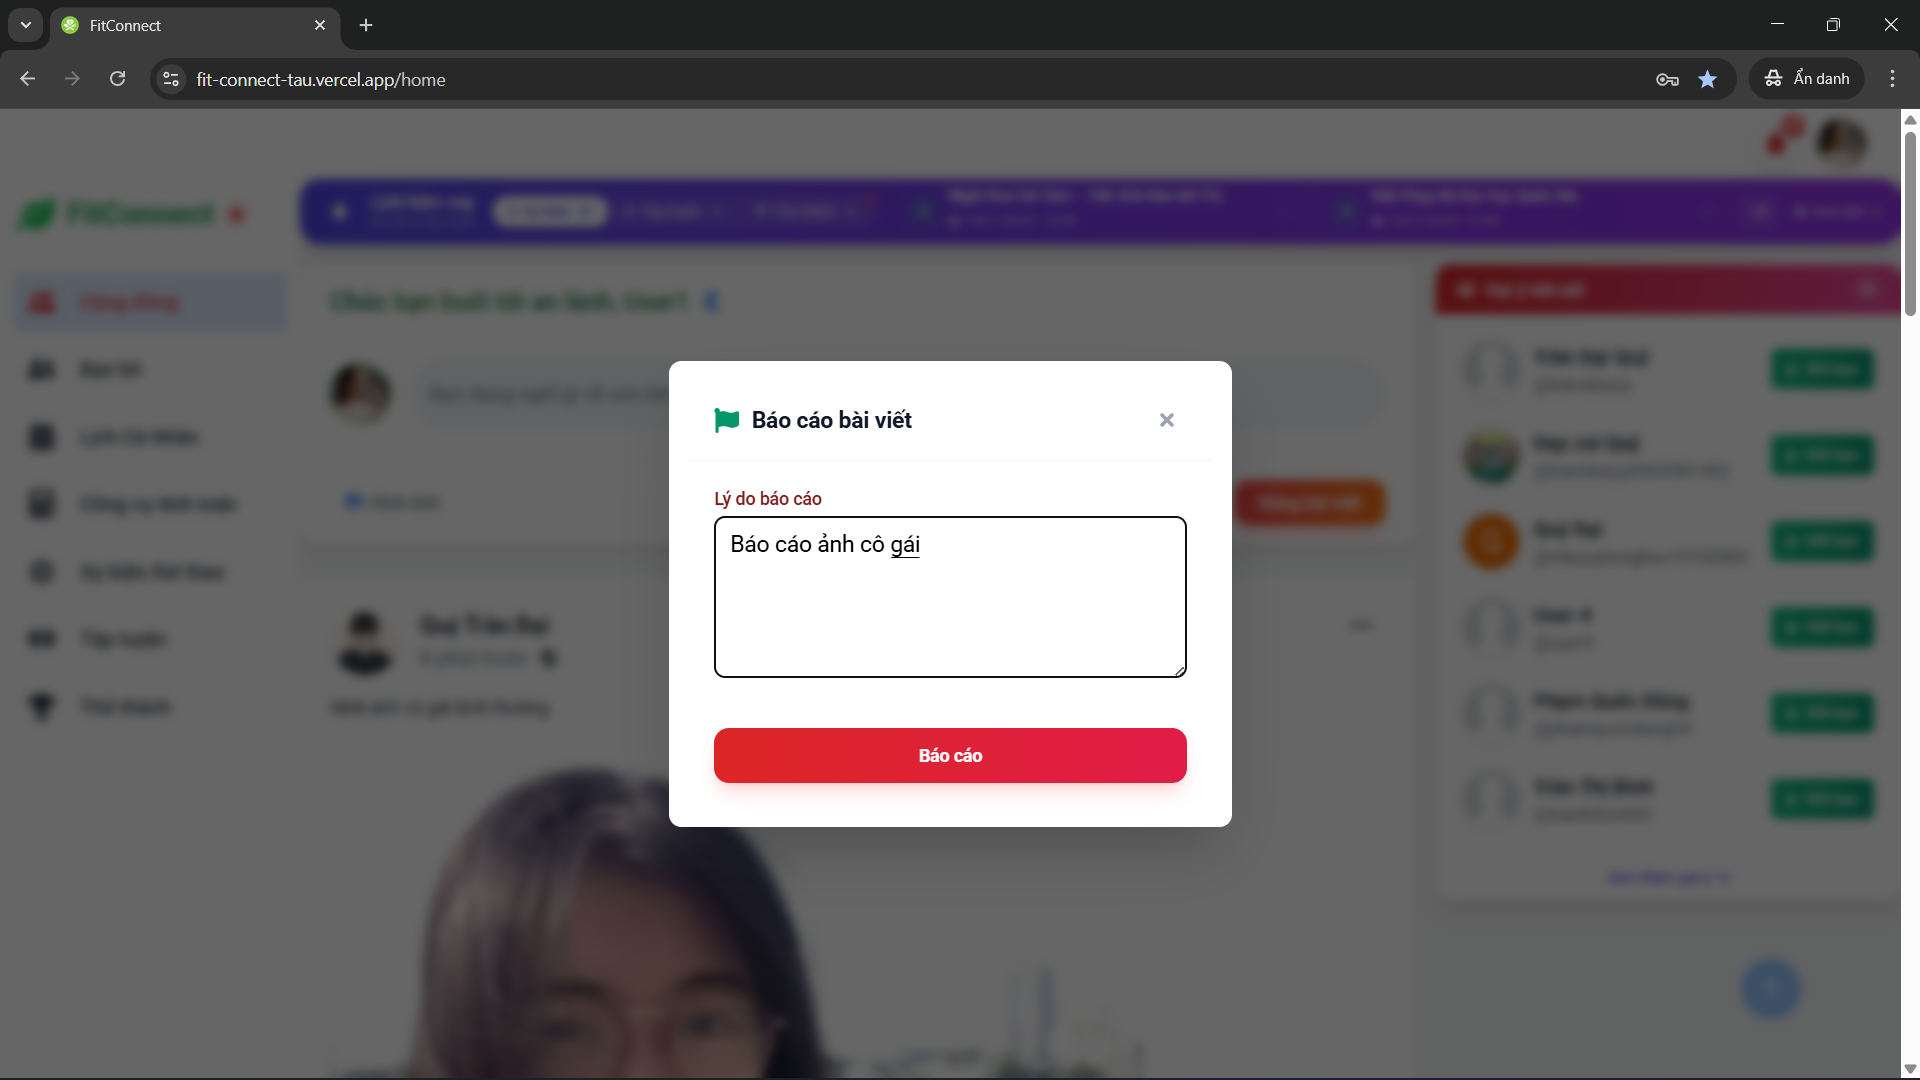
\includegraphics[width=\textwidth]{Images/IMG/Nhom2/modaldienbaocao.png}
        \caption{Hệ thống hiển thị modal tải mẫu điền báo cáo bài viết}
        \label{fig:impl_social_report_modal}
    \end{subfigure}
\end{figure}

\end{itemize}

\subsubsection{Luồng thao tác quản trị bài viết (Góc độ Quản trị viên)}
\begin{itemize}
    \item Quản trị viên xem danh sách bài viết bị báo cáo, đọc nội dung chi tiết và đưa ra quyết định: \textbf{Giữ lại} (bài viết tiếp tục hiển thị, người dùng nhận thông báo) hoặc \textbf{Xóa} (bài viết bị ẩn, chủ bài nhận thông báo vi phạm). Bài viết bị xóa được lưu trong tab ``Đã xóa'' và có thể được khôi phục nếu quản trị viên xem xét lại.

\begin{figure}[H]
    \centering
    \begin{subfigure}[b]{0.47\textwidth}
        \centering
        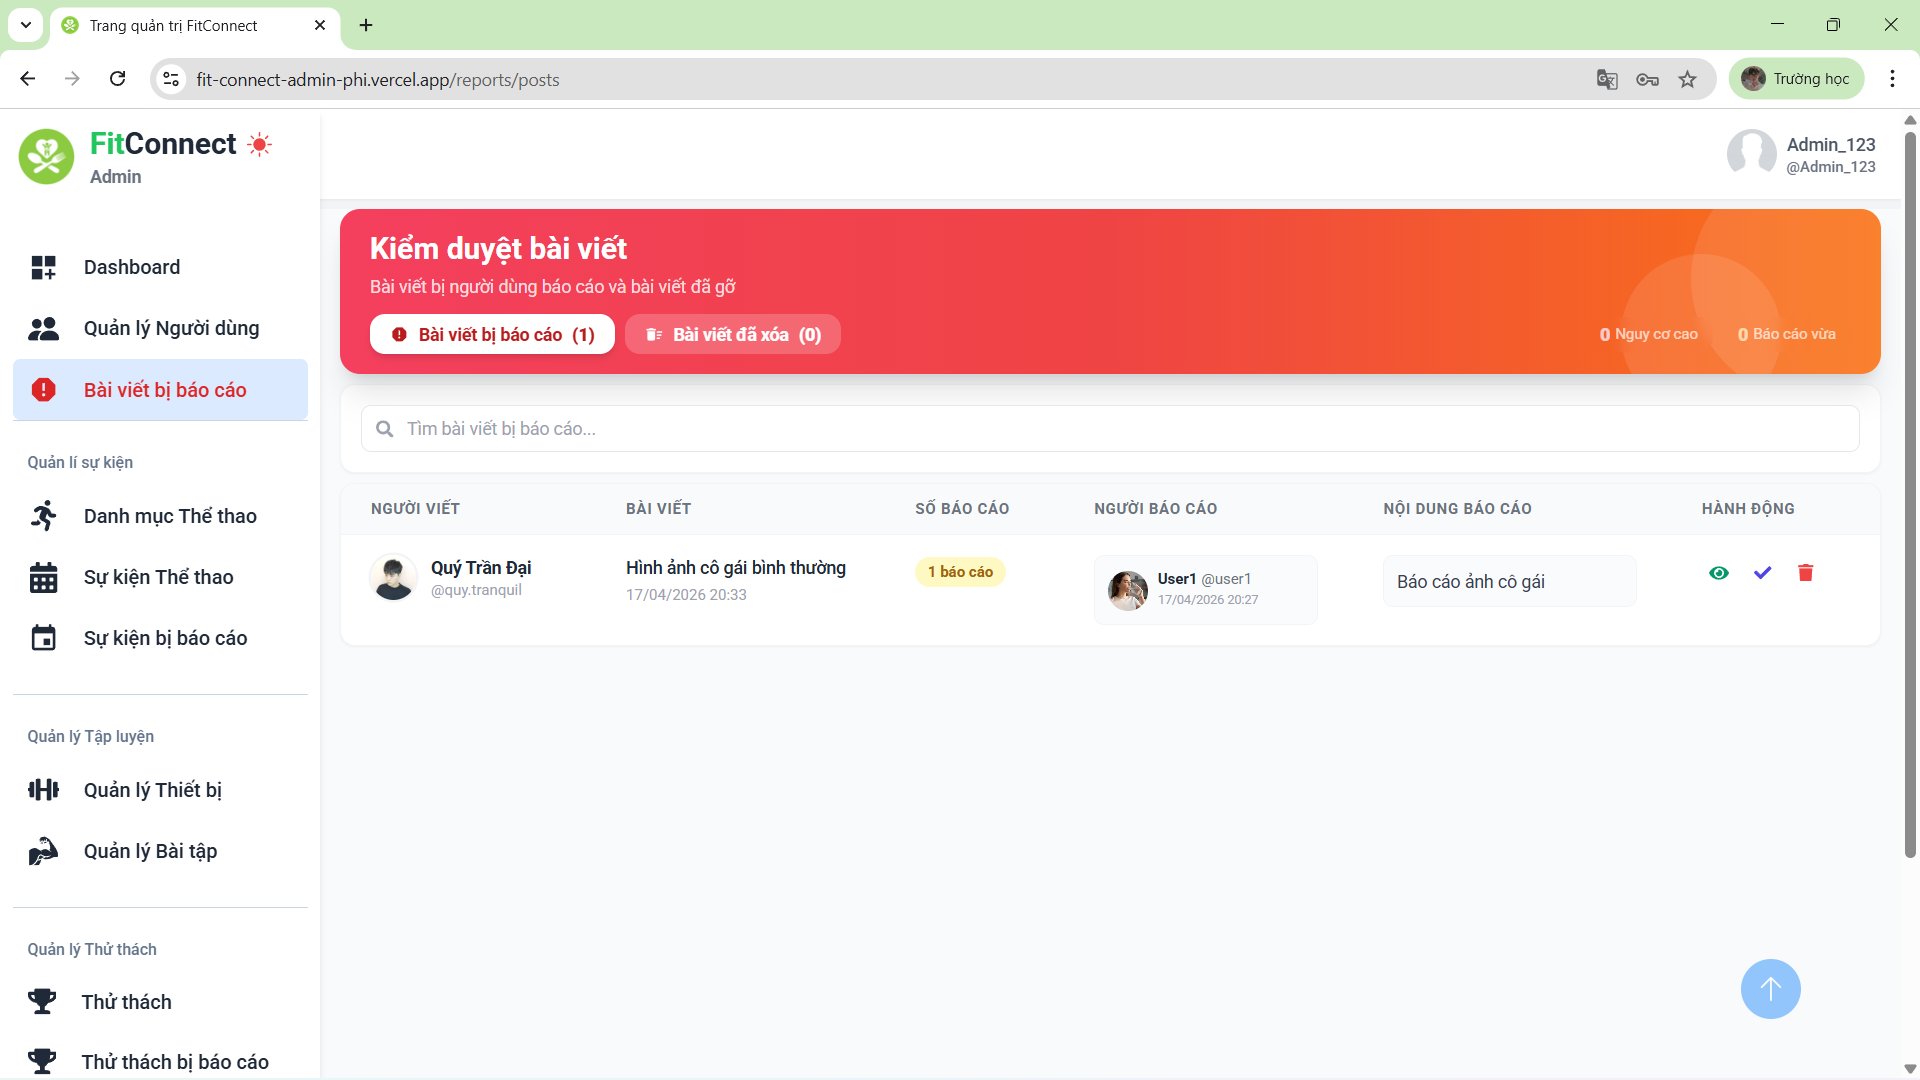
\includegraphics[width=\textwidth]{Images/IMG/Nhom2/hienbaivietbibaocaobenadmin.png}
        \caption{Danh sách bài viết bị báo cáo chờ kiểm duyệt}
        \label{fig:impl_social_admin_receive}
    \end{subfigure}
    \hfill
    \begin{subfigure}[b]{0.47\textwidth}
        \centering
        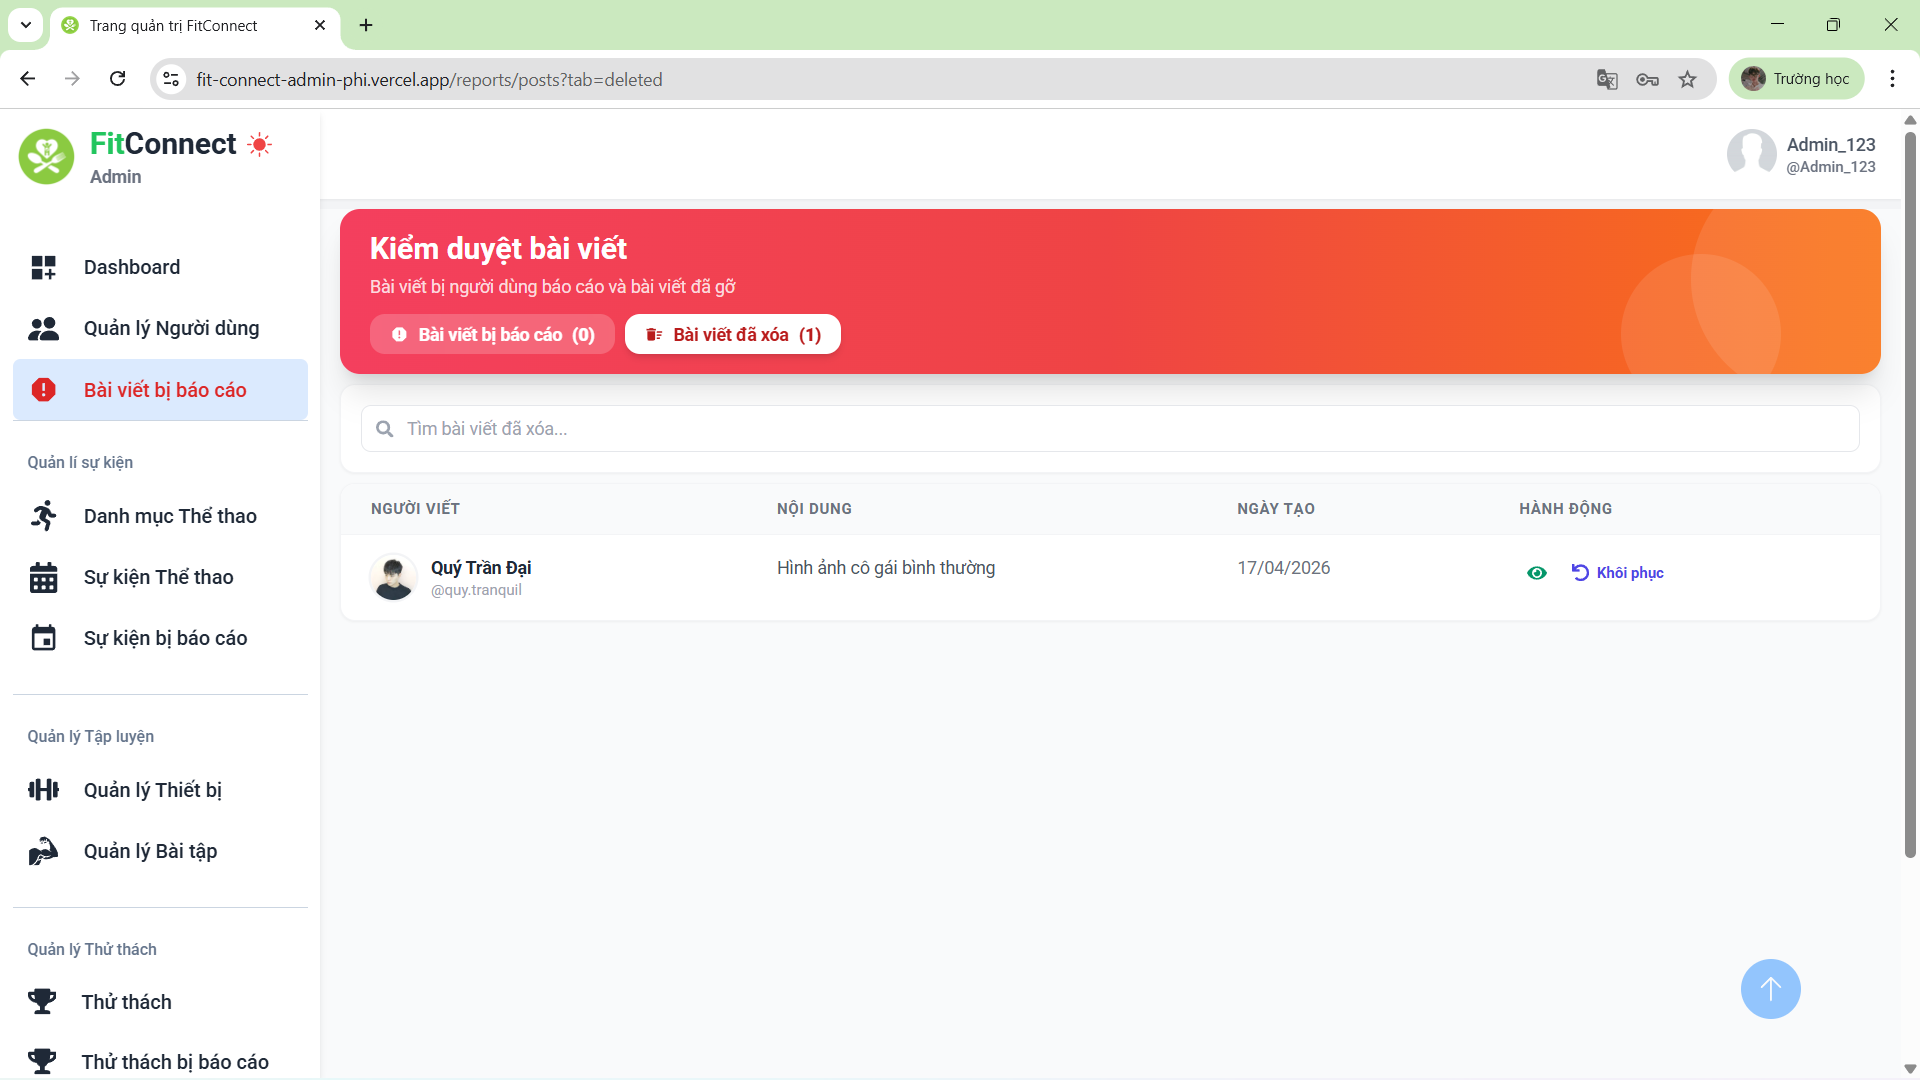
\includegraphics[width=\textwidth]{Images/IMG/Nhom2/hienthibenbaivietbixoa.png}
        \caption{Danh sách bài viết đã xóa và tùy chọn khôi phục}
        \label{fig:impl_social_admin_trash}
    \end{subfigure}
    \vspace{0.3em}
    \caption{Giao diện kiểm duyệt và quản lý bài viết vi phạm của Admin}
    \label{fig:impl_social_admin_moderation}
\end{figure}

\end{itemize}

\subsection{Nhóm tính năng Sự kiện thể thao}
\label{subsec:impl_sport_event}

Nhóm tính năng Sự kiện thể thao cho phép người dùng tổ chức và tham gia các sự kiện thể thao cộng đồng. Hệ thống hỗ trợ hai hình thức tổ chức: Ngoài trời (chạy bộ, đạp xe, leo núi,...) với tính năng theo dõi tiến độ bằng GPS, và Trong nhà (Gym, Yoga, Cardio,...) với tính năng tập luyện qua Video Call có AI theo dõi sự hiện diện. Ngoài ra, hệ thống còn tích hợp AI để hỗ trợ người dùng tạo sự kiện tự động chỉ bằng một đoạn mô tả ngắn.

Quy trình hoạt động gồm ba luồng chính:
\begin{itemize}
    \item \textbf{Người dùng (Người tổ chức):} Tạo, quản lý sự kiện, theo dõi danh sách người tham gia và chỉnh sửa thông tin sự kiện.
    \item \textbf{Người dùng (Người tham gia):} Tìm kiếm, tham gia sự kiện, ghi tiến độ hoạt động, chia sẻ và mời bạn bè.
    \item \textbf{Quản trị viên:} Xử lý các sự kiện bị báo cáo từ cộng đồng.
\end{itemize}

\subsubsection{Luồng thao tác tạo và quản lý sự kiện (Góc độ Người tổ chức)}
\begin{itemize}
    \item Người dùng truy cập trang Sự kiện thể thao, sẽ thấy danh sách các sự kiện thể thao phù hợp nhất kèm theo những sự kiện thể thao nổi bật nhất được hiển thị dạng banner lớn ở đầu trang. Người dùng có thể lọc theo hình thức (Ngoài trời, Trong nhà) và theo danh mục môn thể thao (Cardio, Chạy bộ, Yoga,...).

\begin{figure}[H]
    \centering
    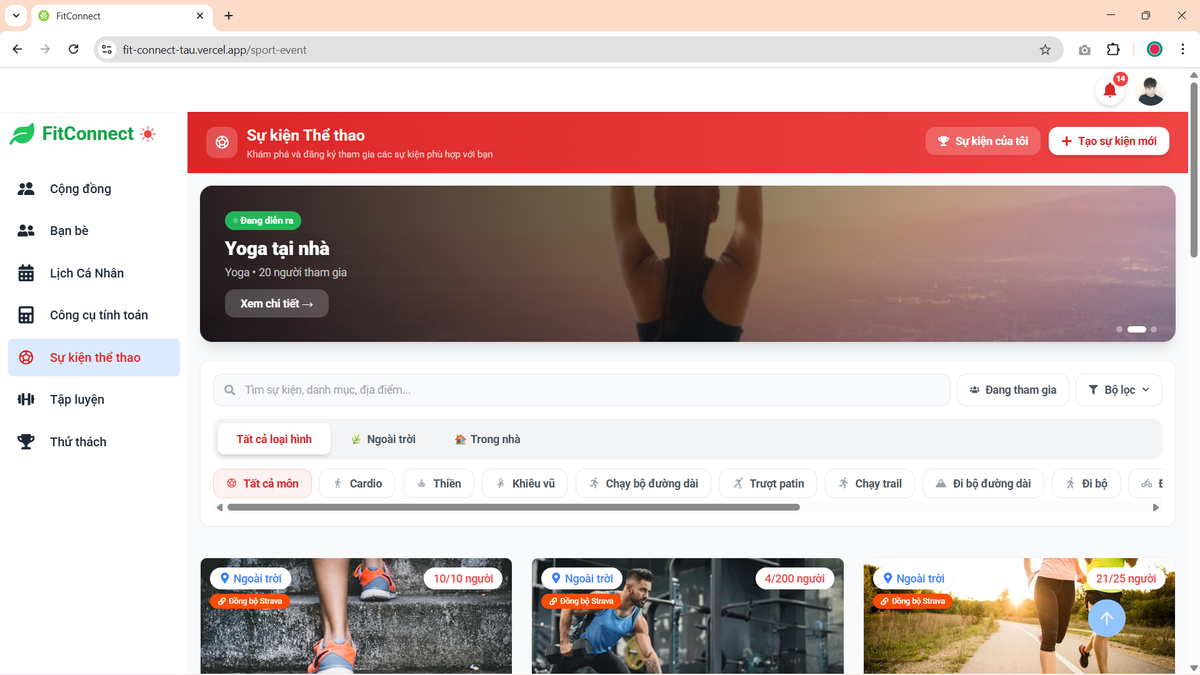
\includegraphics[width=0.60\textwidth]{Images/IMG/nhom3/danhsachsukien.png}
    \caption{Người dùng xem danh sách sự kiện thể thao}
    \label{fig:impl_se_list}
\end{figure}


    \item Người dùng nhấn Tạo sự kiện mới, hệ thống hiển thị trang tạo sự kiện thể thao bao gồm các thông tin: (1) Thông tin chung -- tên sự kiện, danh mục thể thao, hình thức tổ chức (Ngoài trời hoặc Trong nhà); (2) Thời gian \& Địa điểm -- ngày bắt đầu, ngày kết thúc, thời điểm, địa điểm cụ thể; (3) Mục tiêu \& Sức chứa -- số người tối đa, mục tiêu sự kiện (km hoặc kcal); (4) Hình ảnh \& Mô tả -- ảnh bìa, mô tả ngắn, mô tả chi tiết, yêu cầu tham gia, lợi ích khi tham gia.

\begin{figure}[H]
    \centering
    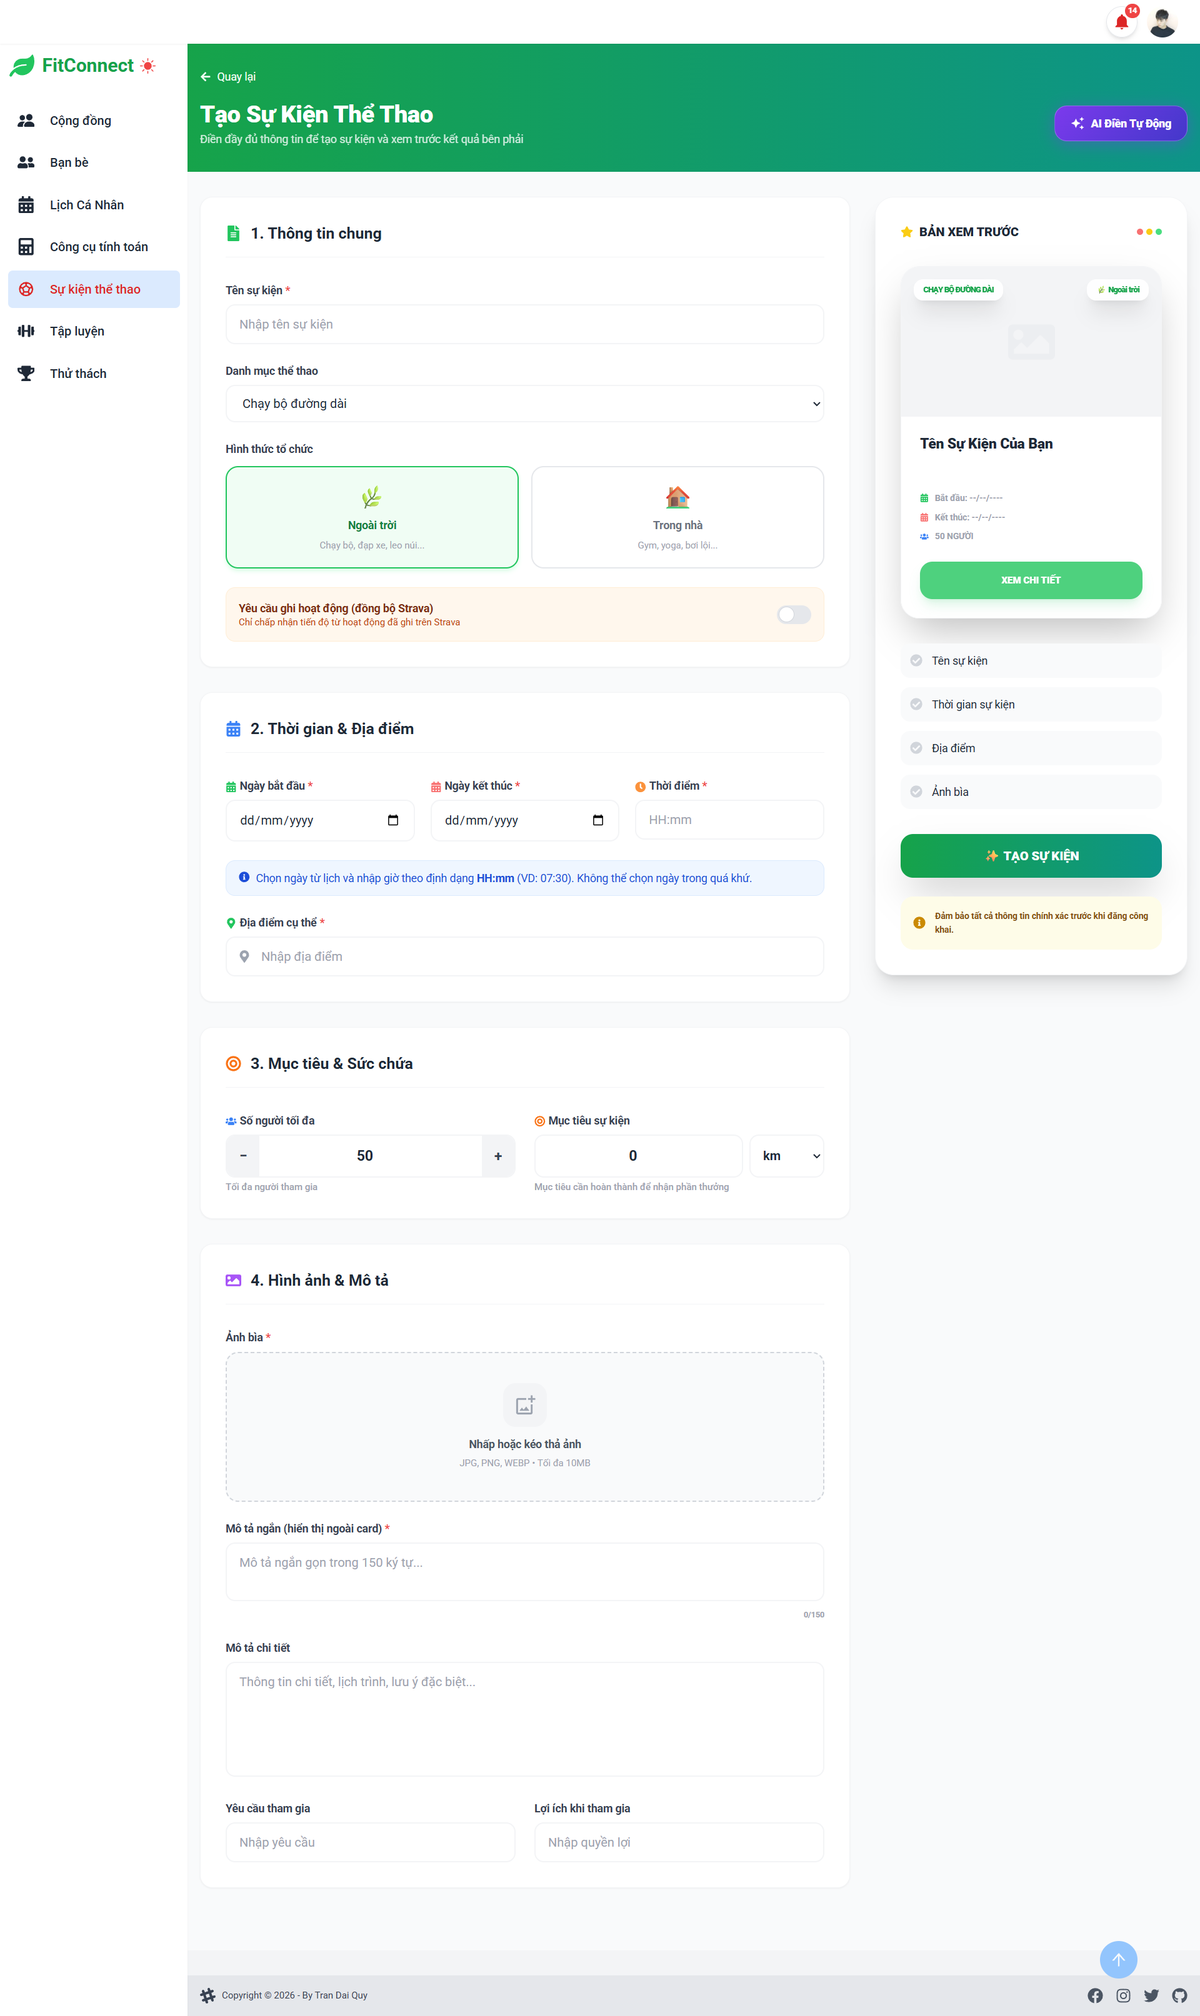
\includegraphics[width=0.60\textwidth]{Images/IMG/nhom3/taosukien.png}
    \caption{Người dùng thao tác tạo sự kiện thể thao mới}
    \label{fig:impl_se_create}
\end{figure}


    \item Người dùng có thể dùng tính năng AI Điền Tự Động để tự động tạo sự kiện thể thao theo yêu cầu. Người dùng chỉ cần mô tả sơ bộ về sự kiện (ví dụ: ``Tạo sự kiện chạy bộ ngoài trời, ở công viên Hoàng Văn Thụ từ 18h hôm nay tới tháng sau''), AI sẽ tự động điền toàn bộ biểu mẫu tạo sự kiện bao gồm tên sự kiện, danh mục, thời gian, địa điểm, mục tiêu và mô tả chi tiết.

\begin{figure}[H]
    \centering
    \begin{subfigure}[b]{0.47\textwidth}
        \centering
        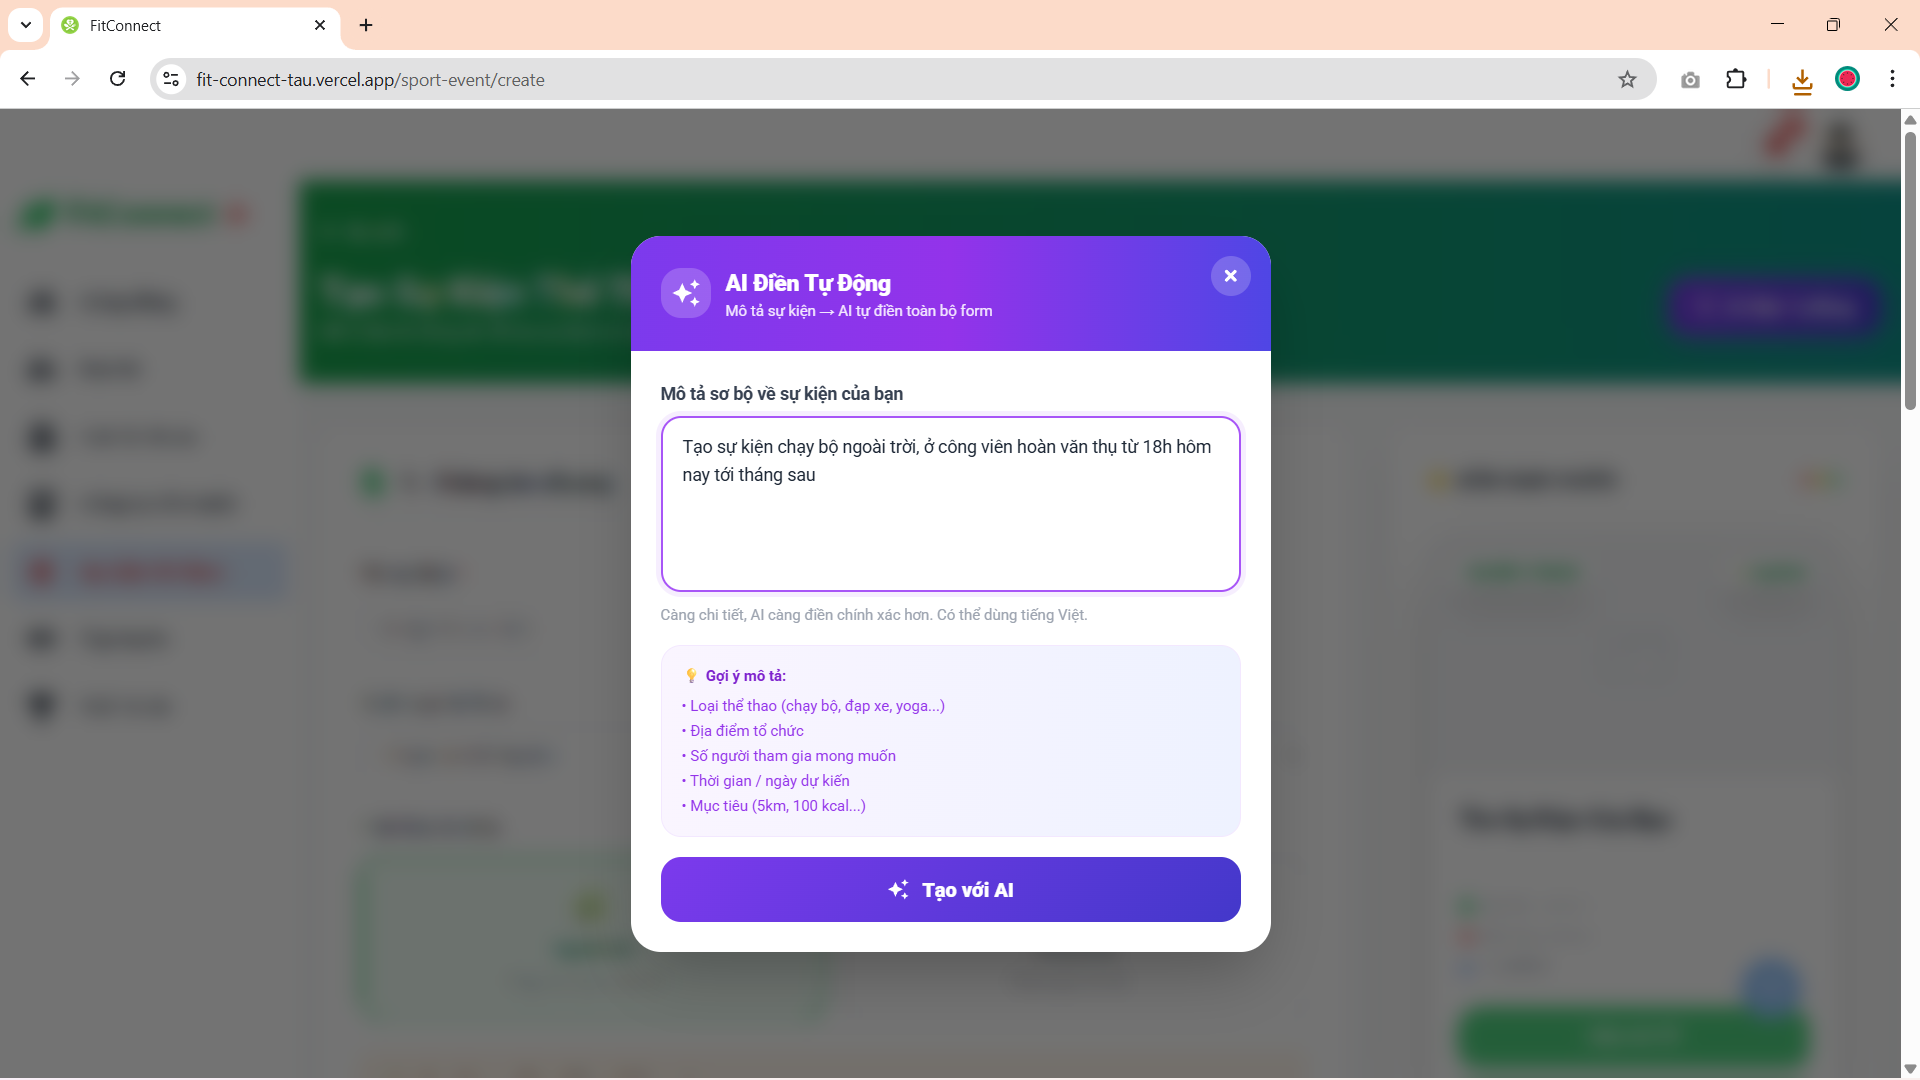
\includegraphics[width=\textwidth]{Images/IMG/nhom3/modaldienAItaosukientudong.png}
        \caption{Hệ thống hiển thị modal AI Điền Tự Động tạo sự kiện}
        \label{fig:impl_se_ai_modal}
    \end{subfigure}
    \hfill
    \begin{subfigure}[b]{0.47\textwidth}
        \centering
        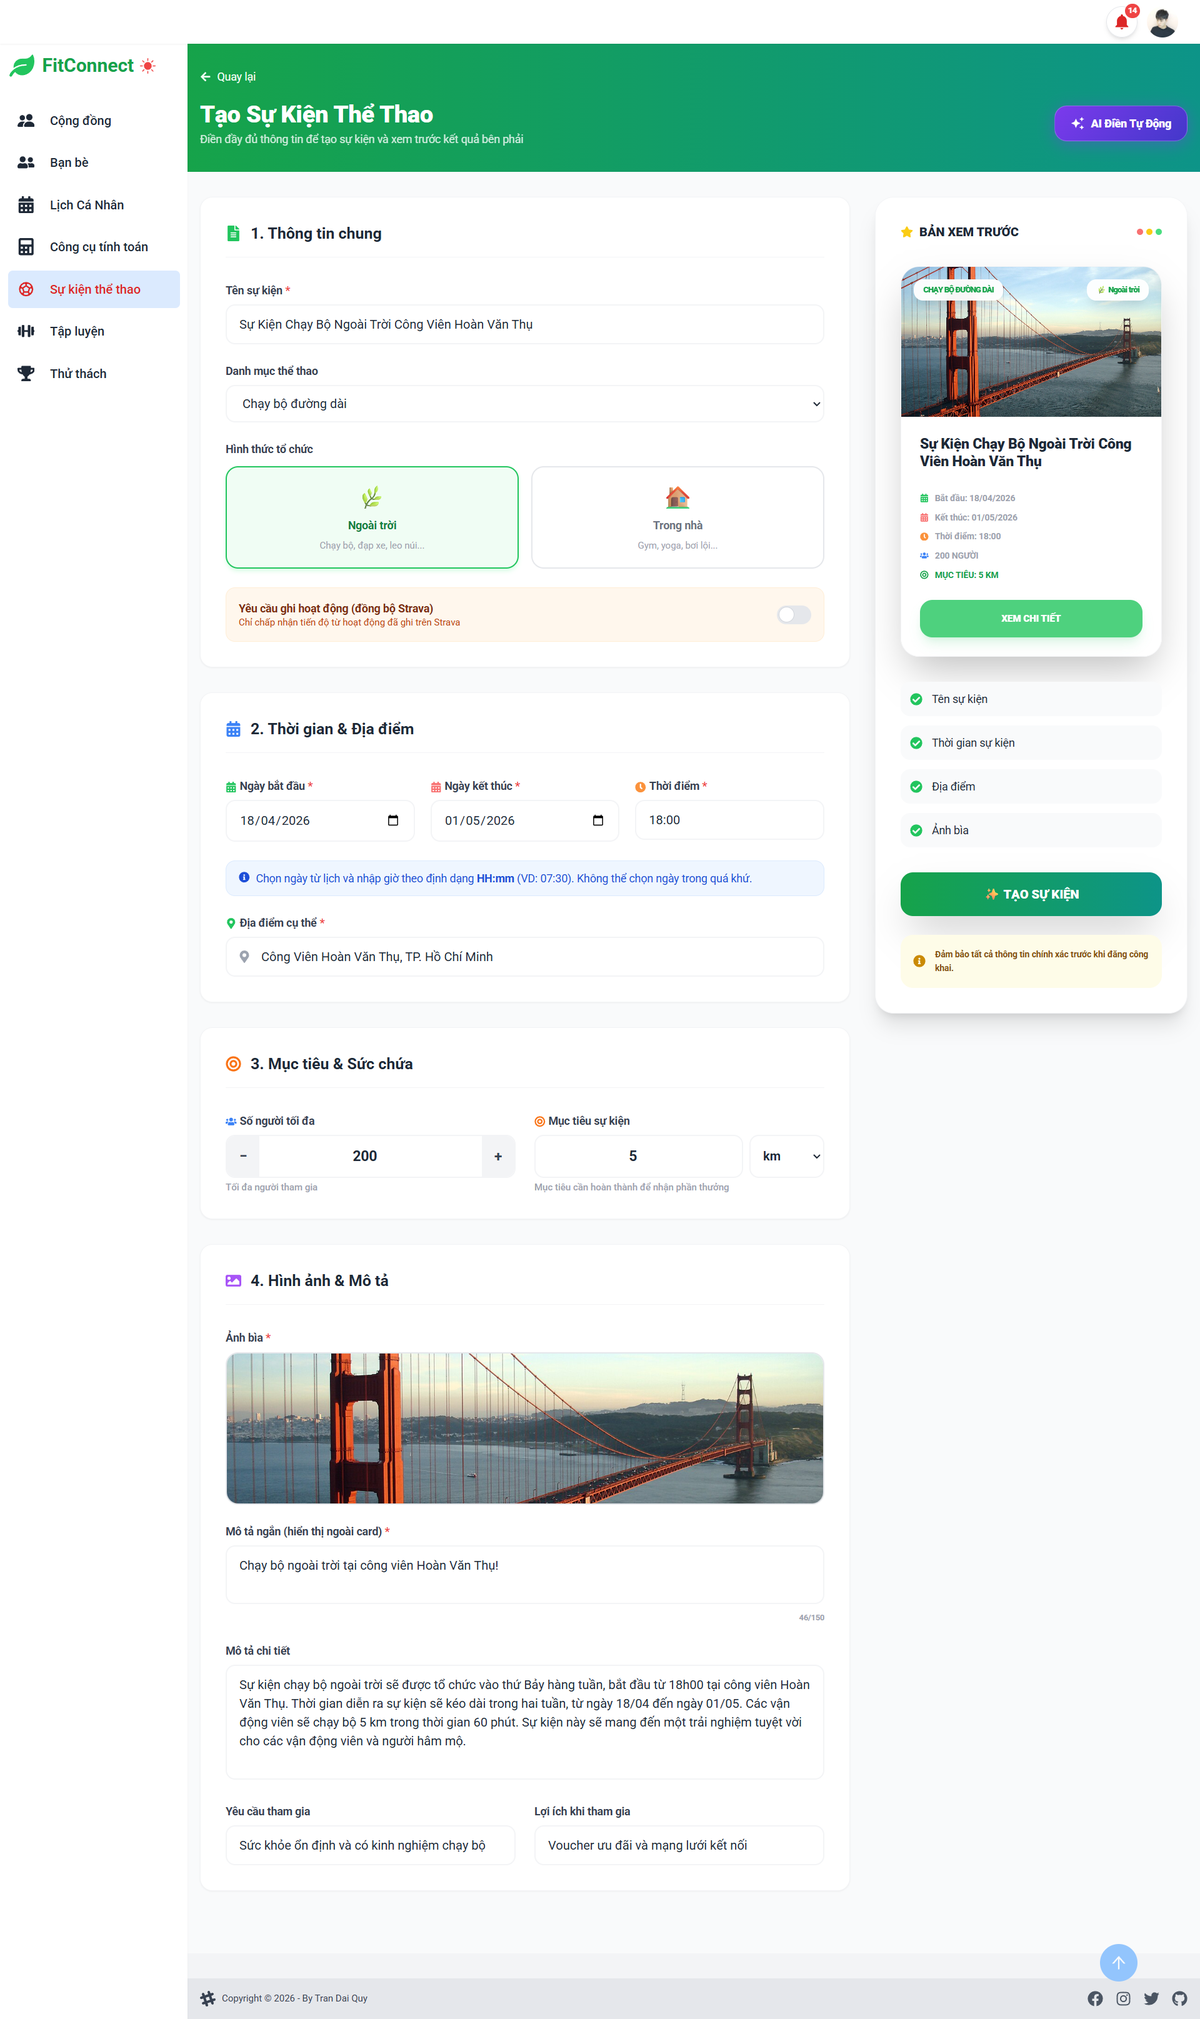
\includegraphics[width=\textwidth]{Images/IMG/nhom3/taobangAIthanhcong.png}
        \caption{Hệ thống tự động điền thông tin sự kiện sau khi AI xử lý thành công}
        \label{fig:impl_se_ai_success}
    \end{subfigure}
\end{figure}


    \item Sau khi nhấn Tạo sự kiện, hệ thống tự động điều hướng đến trang chi tiết sự kiện vừa tạo (người tạo đã được đăng ký tham gia mặc định). Tại trang ``Sự kiện của tôi'', người dùng quản lý được toàn bộ sự kiện đã tạo và đã tham gia.

\begin{figure}[H]
    \centering
    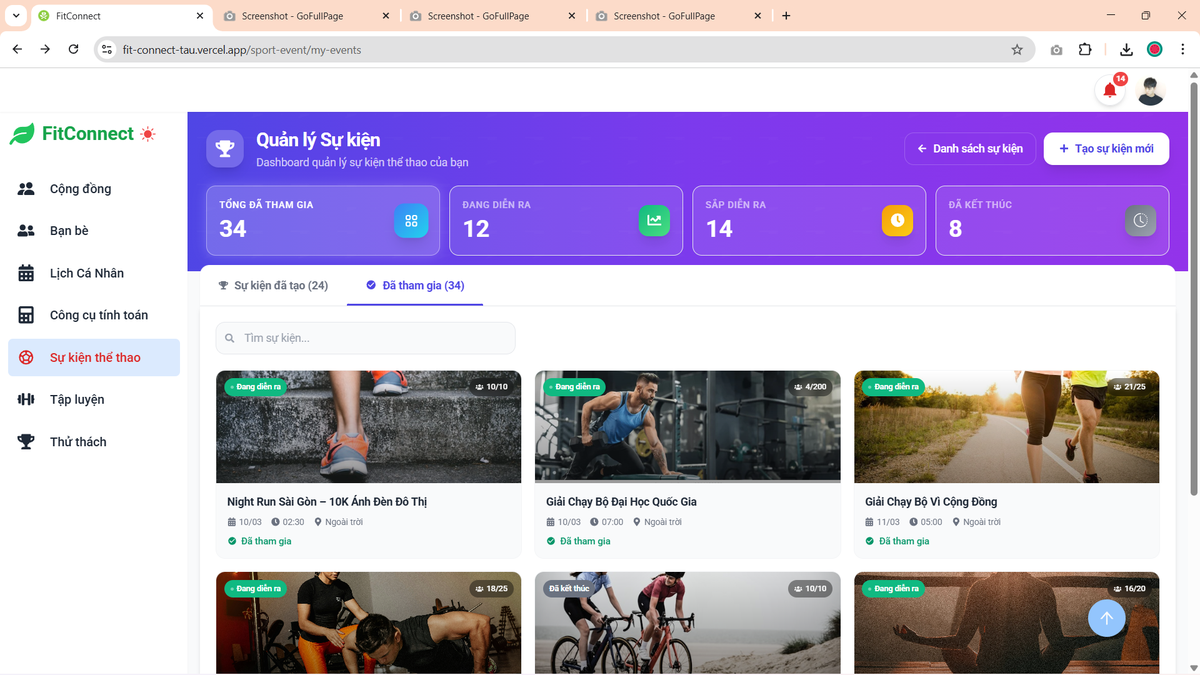
\includegraphics[width=0.60\textwidth]{Images/IMG/nhom3/quanlysukien.png}
    \caption{Người dùng xem trang quản lý sự kiện của tôi}
    \label{fig:impl_se_my_events}
\end{figure}


    \begin{itemize}
        \item Với những sự kiện đã tạo, người tổ chức có thể xem tổng quan sự kiện, xem danh sách những người tham gia (theo dõi tiến độ, xóa/sửa danh sách), và xem cài đặt sự kiện.

\begin{figure}[H]
    \centering
    \begin{subfigure}[b]{0.30\textwidth}
        \centering
        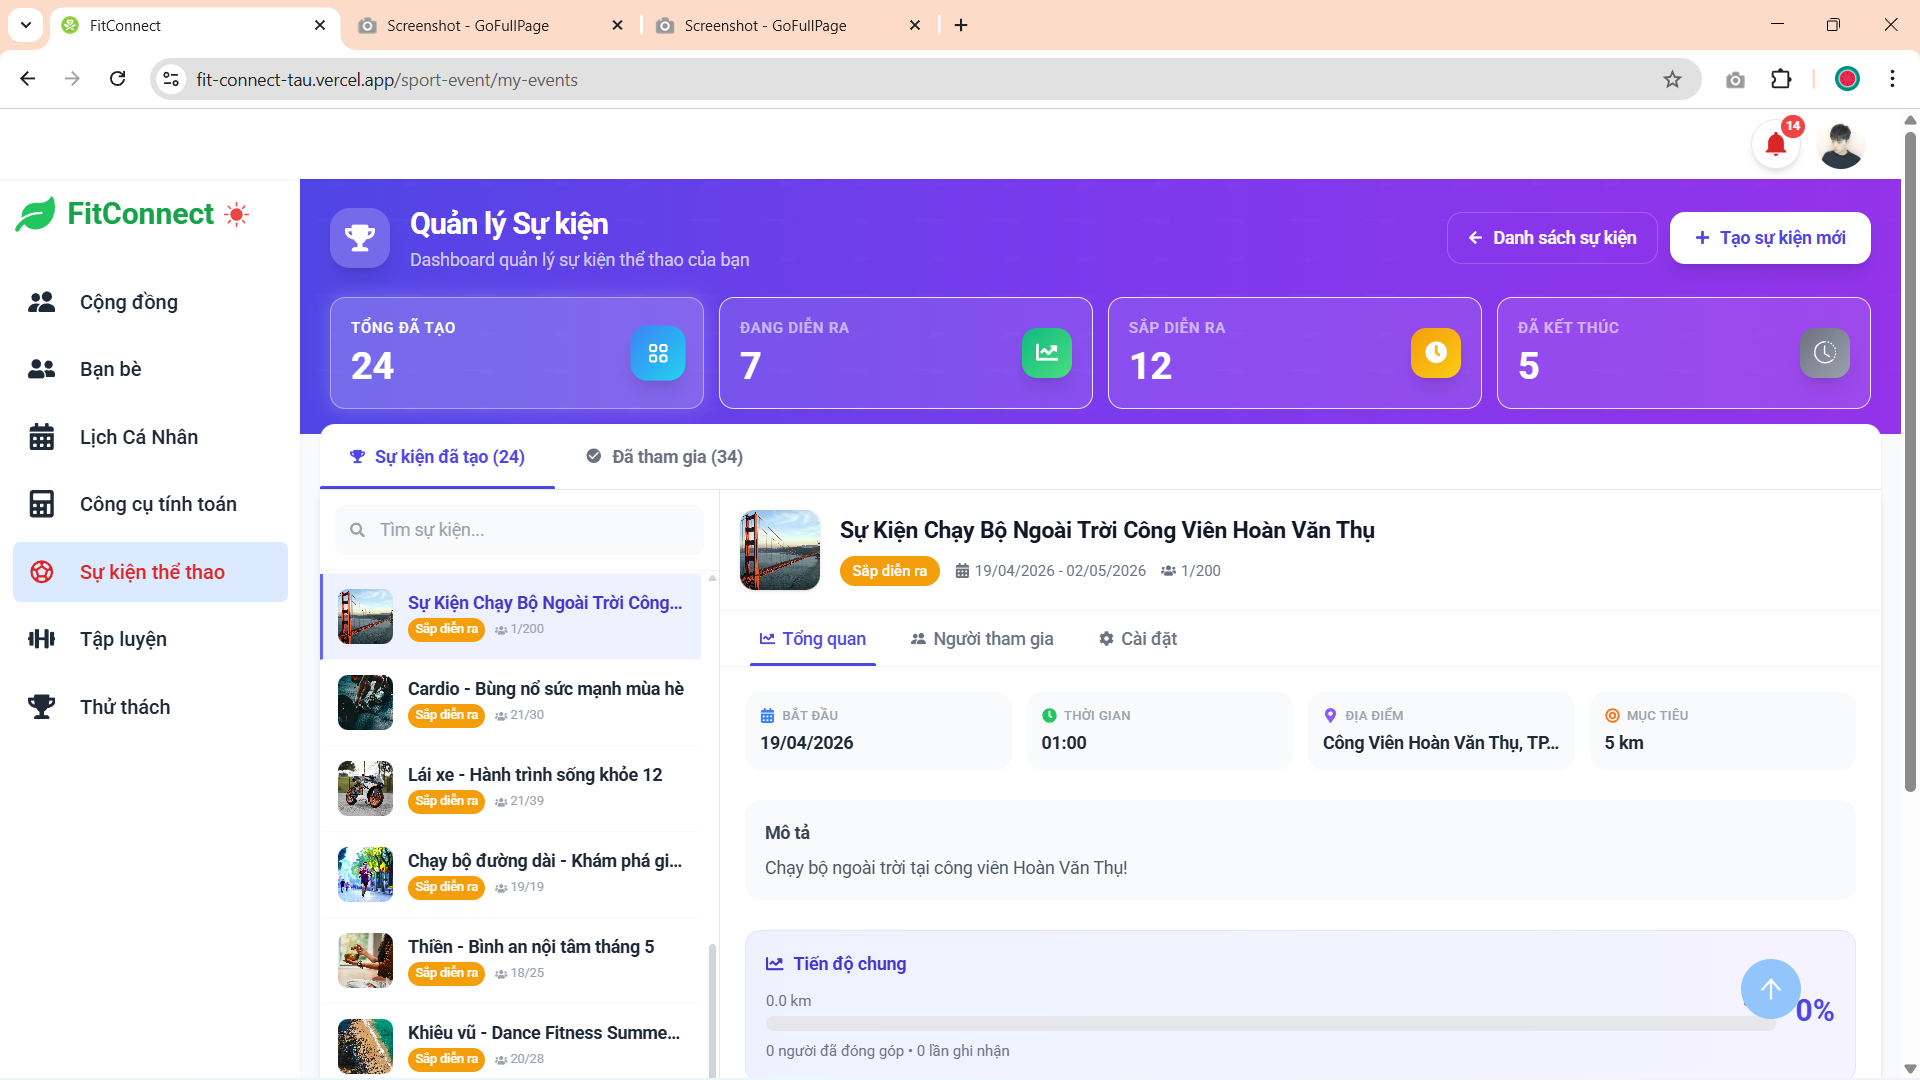
\includegraphics[width=\textwidth]{Images/IMG/nhom3/trangquanlysukienvatongquansk.png}
        \caption{Người tổ chức xem trang quản lý sự kiện và tổng quan sự kiện}
        \label{fig:impl_se_overview}
    \end{subfigure}
    \hfill
    \begin{subfigure}[b]{0.30\textwidth}
        \centering
        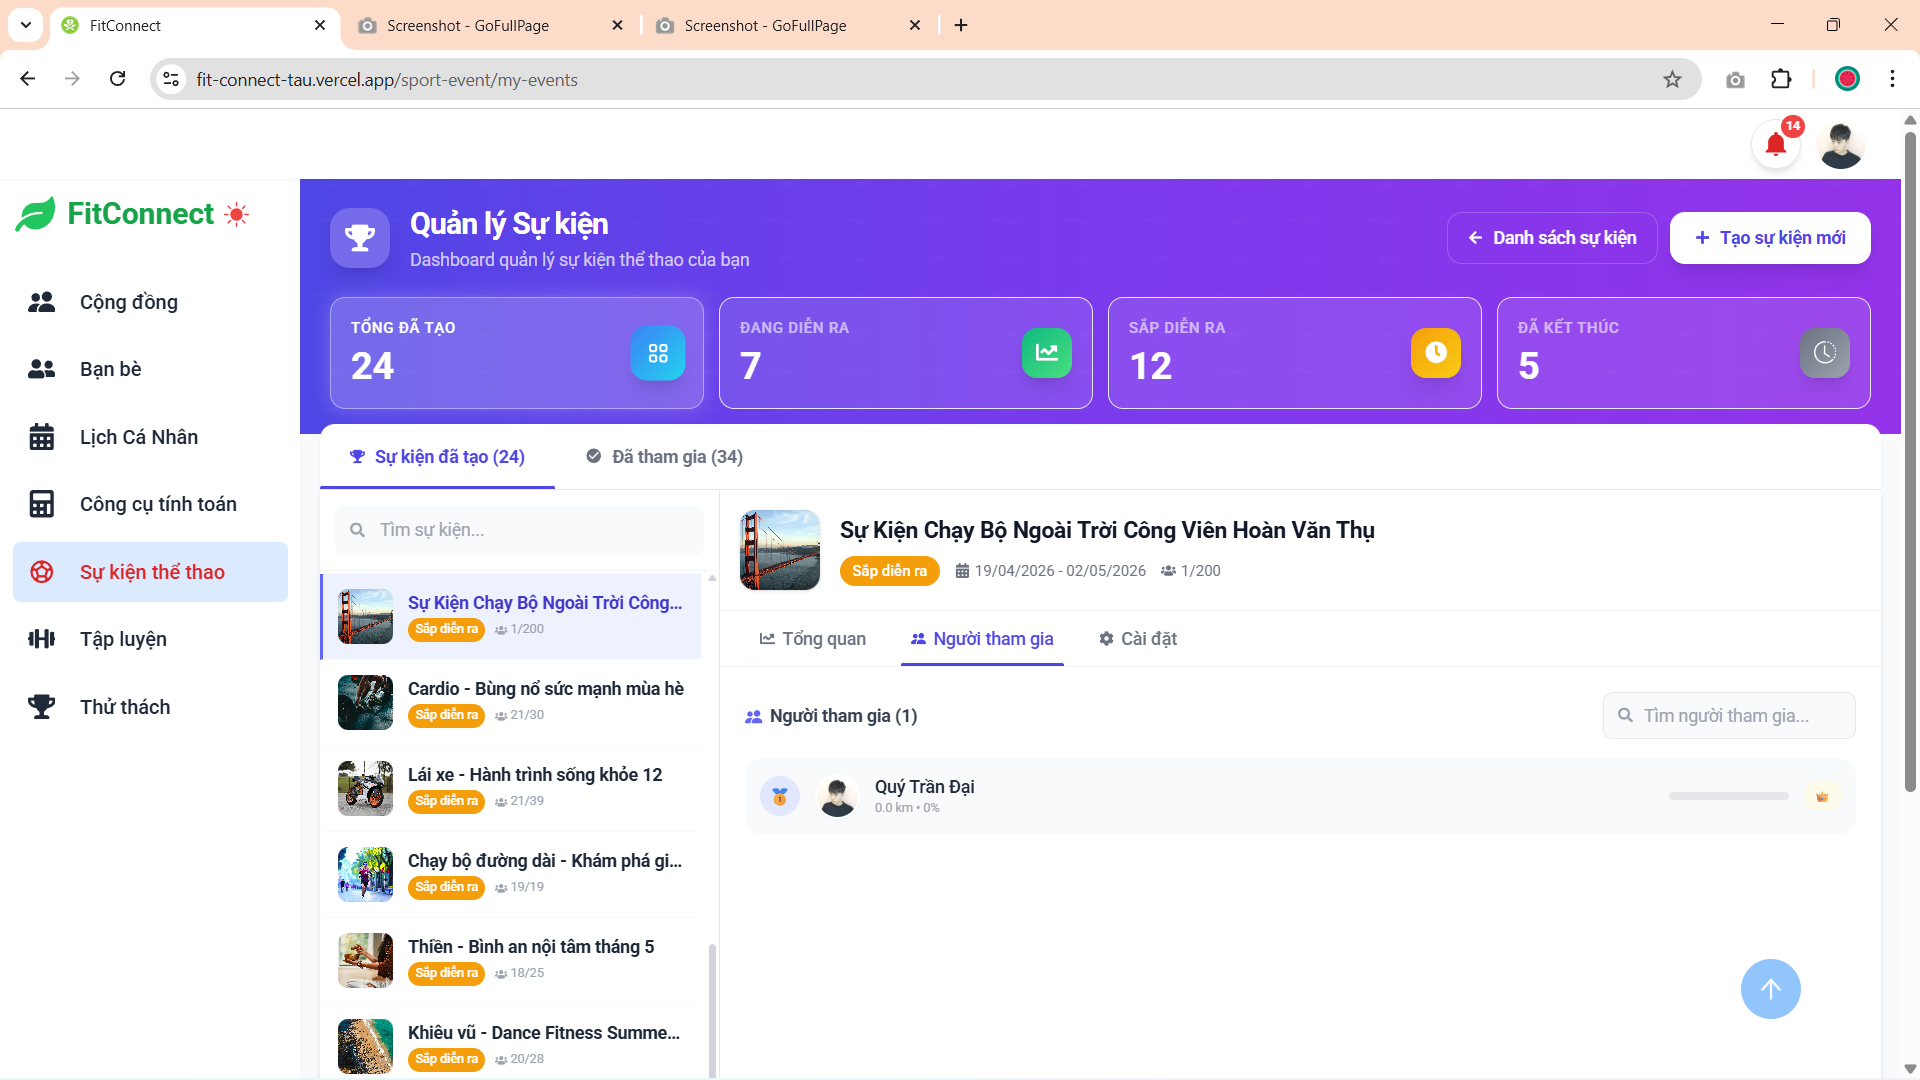
\includegraphics[width=\textwidth]{Images/IMG/nhom3/nguoithamgiasukientoidatao.png}
        \caption{Người tổ chức xem danh sách người tham gia sự kiện đã tạo}
        \label{fig:impl_se_participants}
    \end{subfigure}
    \hfill
    \begin{subfigure}[b]{0.30\textwidth}
        \centering
        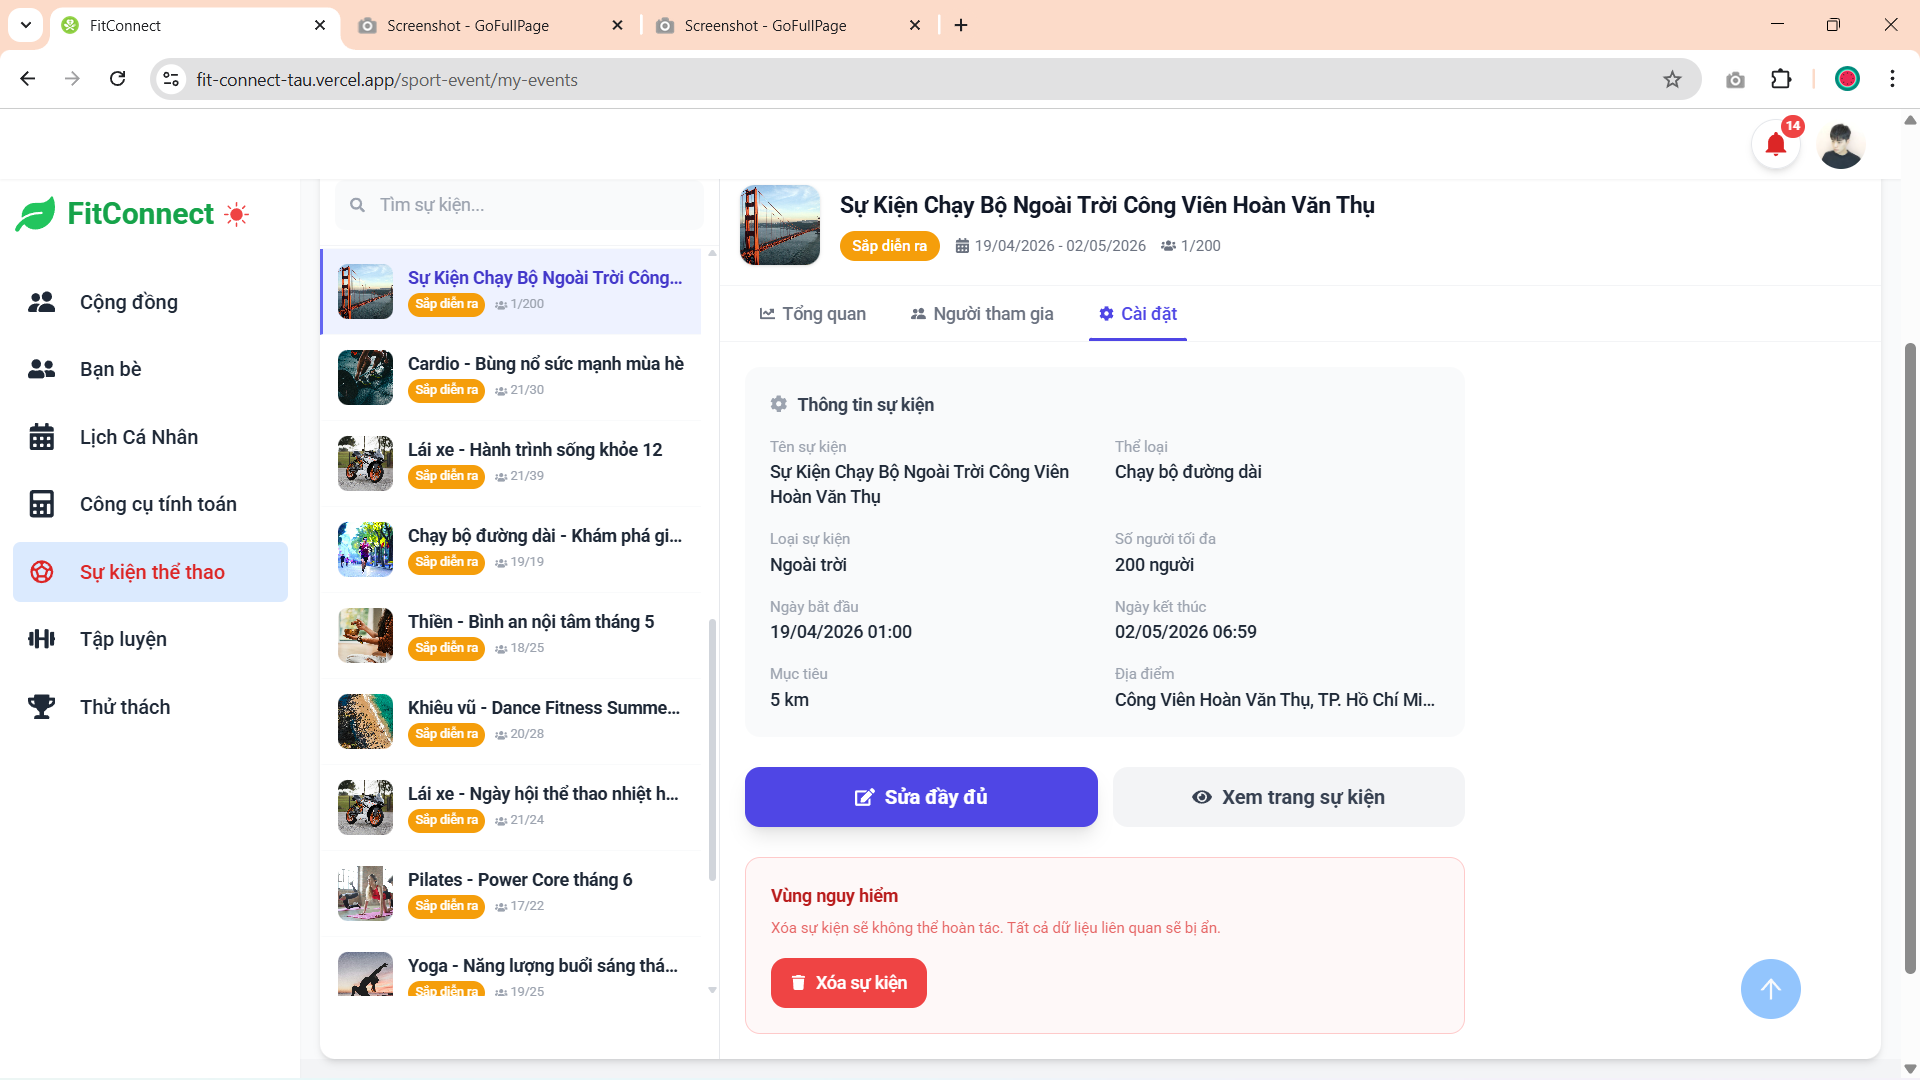
\includegraphics[width=\textwidth]{Images/IMG/nhom3/caidatsukientoidatao.png}
        \caption{Người tổ chức xem cài đặt sự kiện đã tạo}
        \label{fig:impl_se_settings}
    \end{subfigure}
\end{figure}


        \item Với chỉnh sửa sự kiện: Người tổ chức có thể chỉnh sửa thông tin sự kiện và nhấn Lưu để cập nhật, dữ liệu sự kiện sẽ được cập nhật theo những chỉnh sửa mới nhất.

\begin{figure}[H]
    \centering
    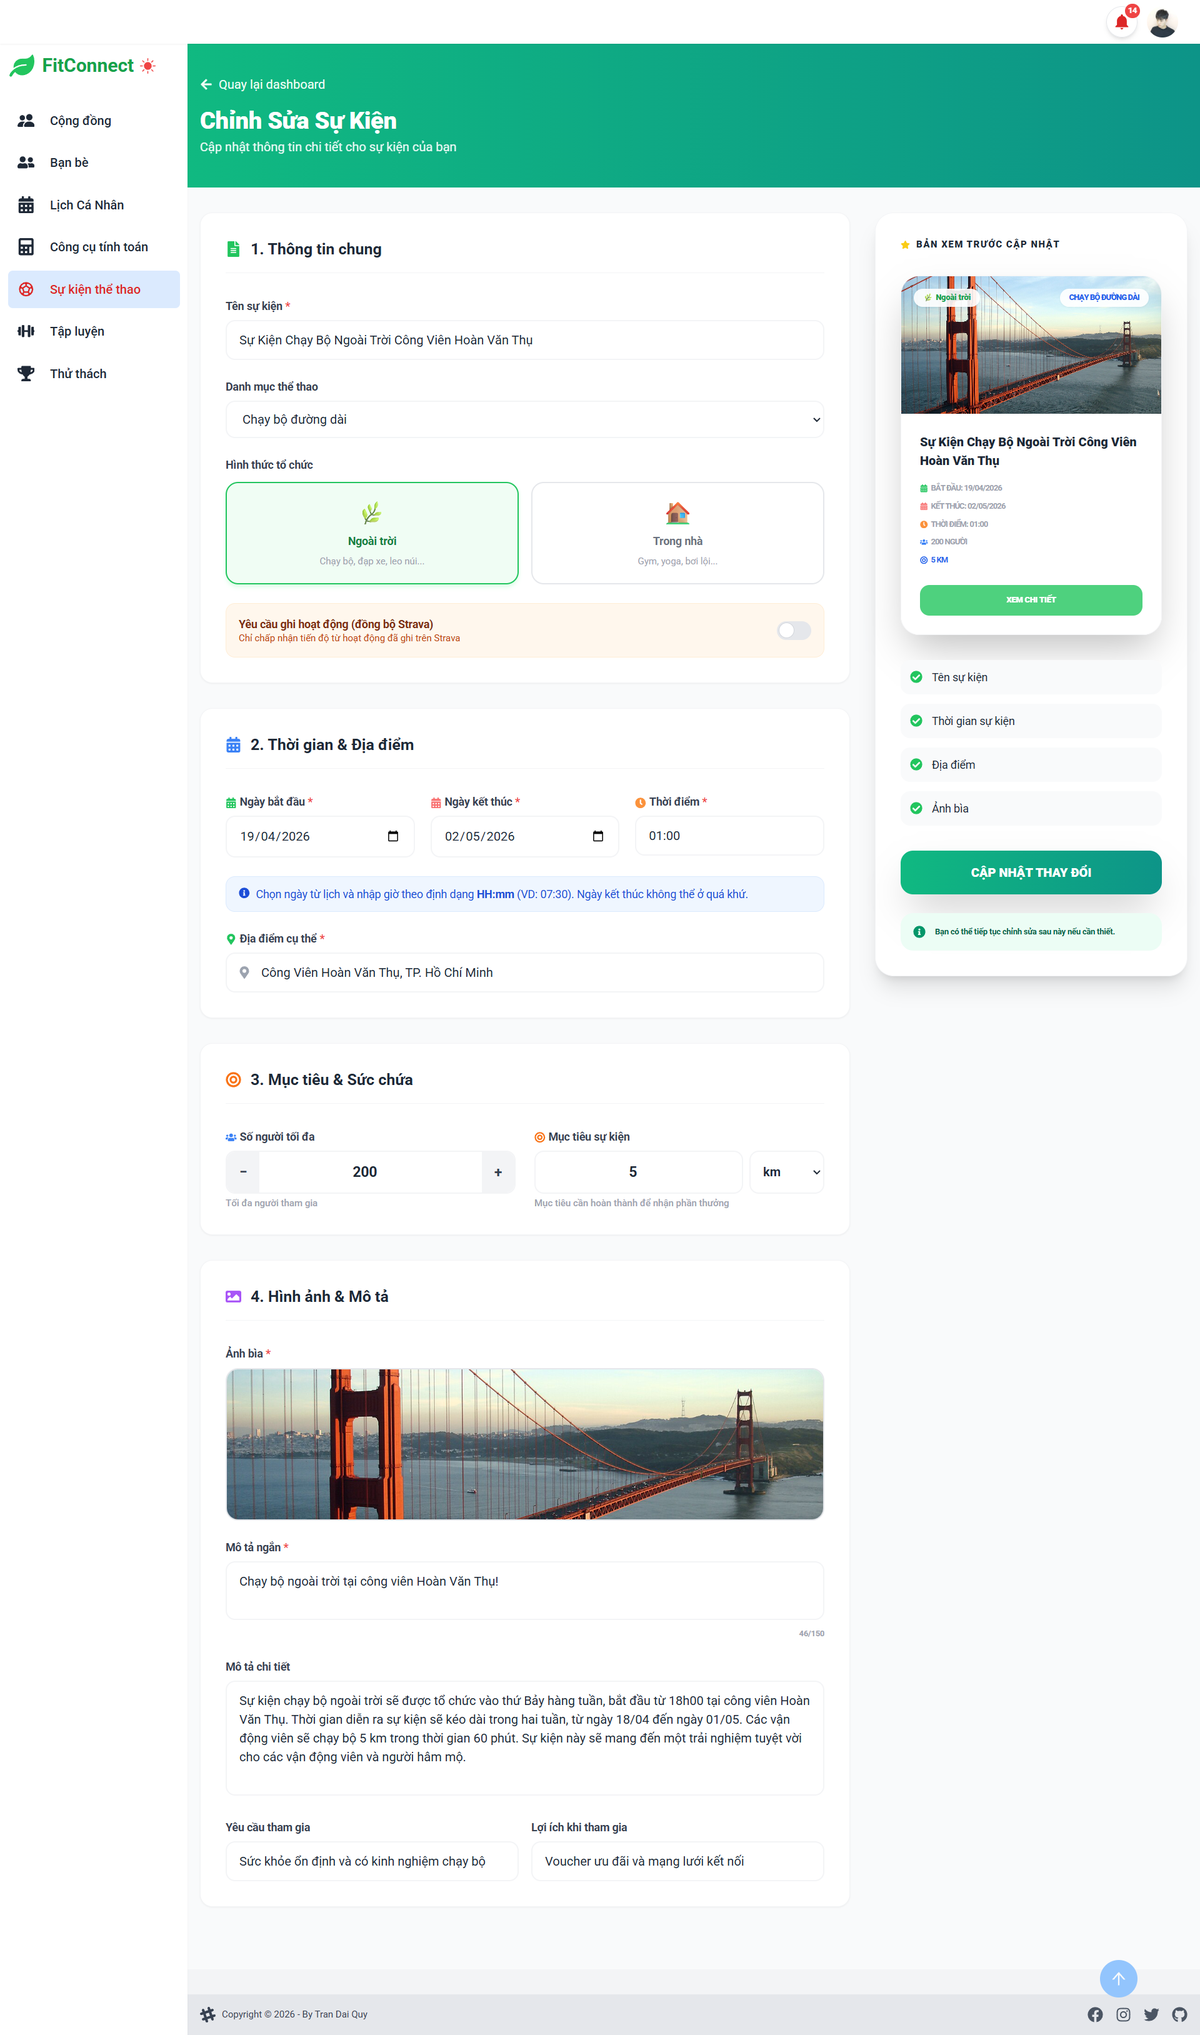
\includegraphics[width=0.60\textwidth]{Images/IMG/nhom3/chinhsuasukiencuatoi.png}
    \caption{Người tổ chức thao tác chỉnh sửa sự kiện của tôi}
    \label{fig:impl_se_edit}
\end{figure}


        \item Với xóa sự kiện: Người tổ chức có thể xóa sự kiện khi sự kiện chưa bắt đầu; hệ thống thực hiện xóa mềm (đánh dấu đã xóa), sự kiện không còn hiển thị phía người dùng nhưng vẫn được lưu trong dữ liệu hệ thống để Admin có thể khôi phục.

    \end{itemize}
\end{itemize}

\subsubsection{Luồng thao tác tham gia sự kiện (Góc độ Người tham gia)}
\begin{itemize}
    \item Với người dùng không phải là người tổ chức, ở trang danh sách sự kiện có thể lọc và tìm kiếm sự kiện để tham gia. Khi nhấn tham gia sự kiện, hệ thống sẽ chuyển đến trang chi tiết sự kiện hiển thị toàn bộ thông tin bao gồm: mô tả sự kiện, thời gian, địa điểm, mục tiêu, tiến độ tổng quan của nhóm, thống kê sự kiện, bảng xếp hạng và danh sách người tham gia.

\begin{figure}[H]
    \centering
    \begin{subfigure}[b]{0.47\textwidth}
        \centering
        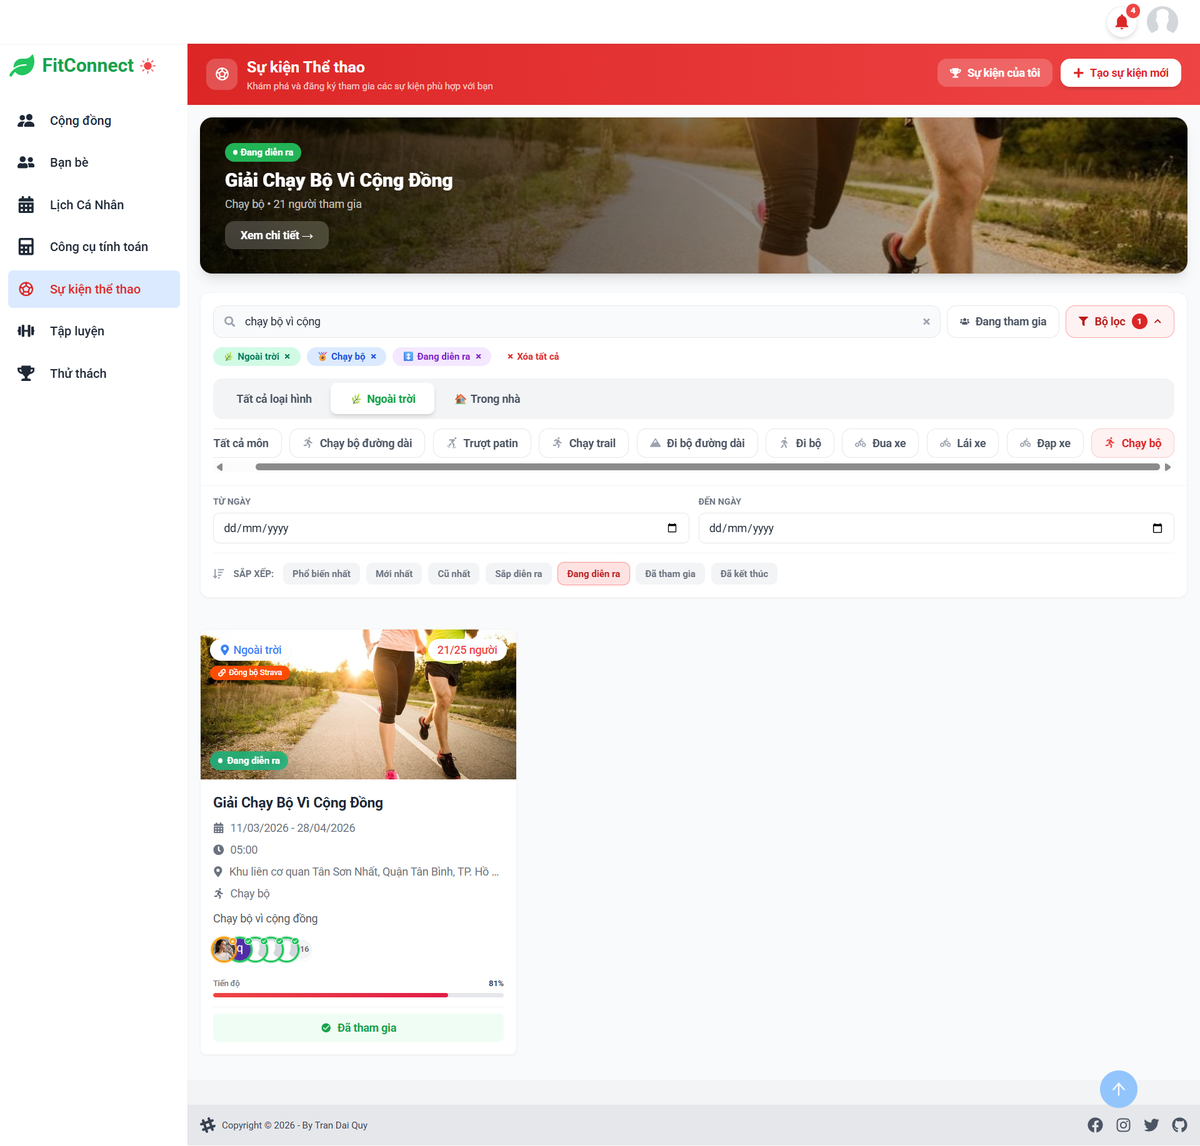
\includegraphics[width=\textwidth]{Images/IMG/nhom3/timkiemsukienvathamgiasukien.png}
        \caption{Người dùng thao tác tìm kiếm và tham gia sự kiện}
        \label{fig:impl_se_search_join}
    \end{subfigure}
    \hfill
    \begin{subfigure}[b]{0.47\textwidth}
        \centering
        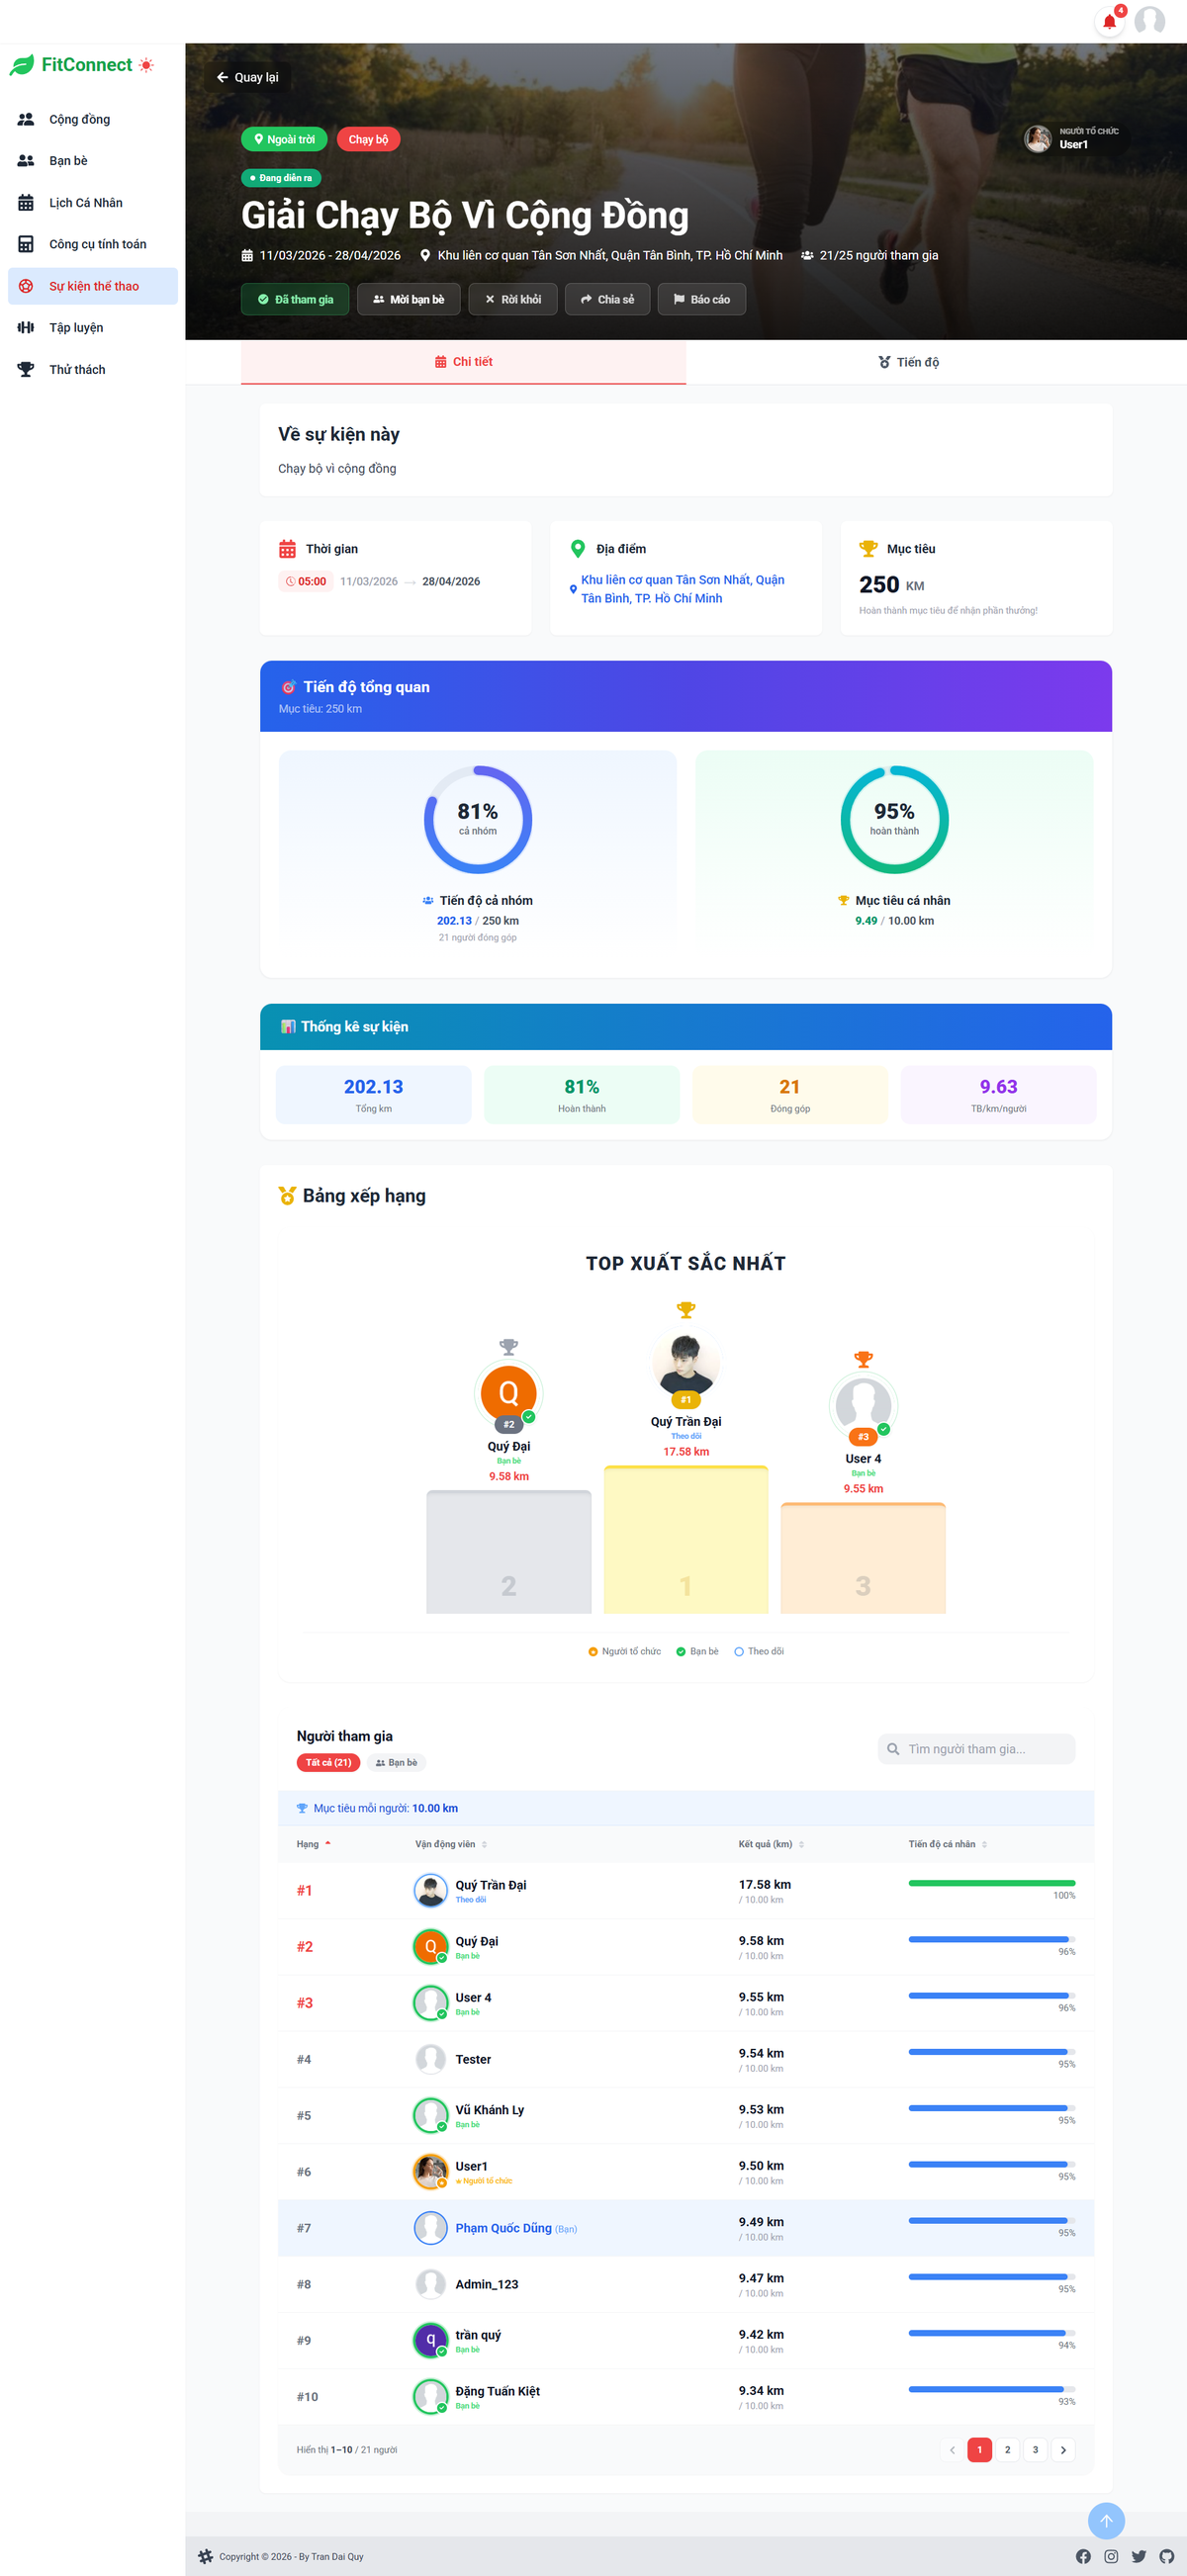
\includegraphics[width=\textwidth]{Images/IMG/nhom3/thongtinchitietsukien.png}
        \caption{Hệ thống hiển thị thông tin chi tiết sự kiện thể thao}
        \label{fig:impl_se_detail}
    \end{subfigure}
\end{figure}


    \item Người tham gia có thể chia sẻ sự kiện lên trang Cộng đồng để lan tỏa và mời thêm người tham gia; bài viết sự kiện sẽ tự động xuất hiện trên Bảng tin.

\begin{figure}[H]
    \centering
    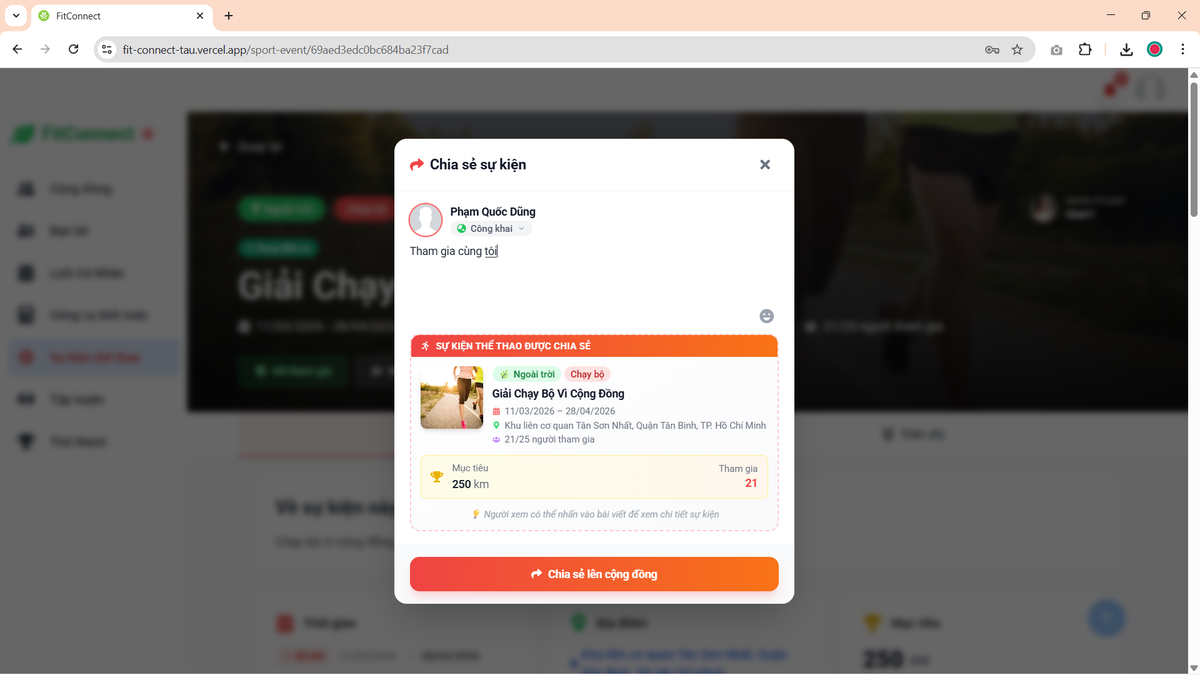
\includegraphics[width=0.60\textwidth]{Images/IMG/nhom3/chiasesukienngoaitroi.png}
    \caption{Người tham gia thao tác chia sẻ sự kiện ngoài trời lên cộng đồng}
    \label{fig:impl_se_share}
\end{figure}


    \item Người tham gia có thể mời bạn bè tham gia sự kiện. Người được mời sẽ nhận thông báo được mời tham gia sự kiện, nhấn vào thông báo sẽ chuyển đến trang sự kiện được mời.

\begin{figure}[H]
    \centering
    \begin{subfigure}[b]{0.47\textwidth}
        \centering
        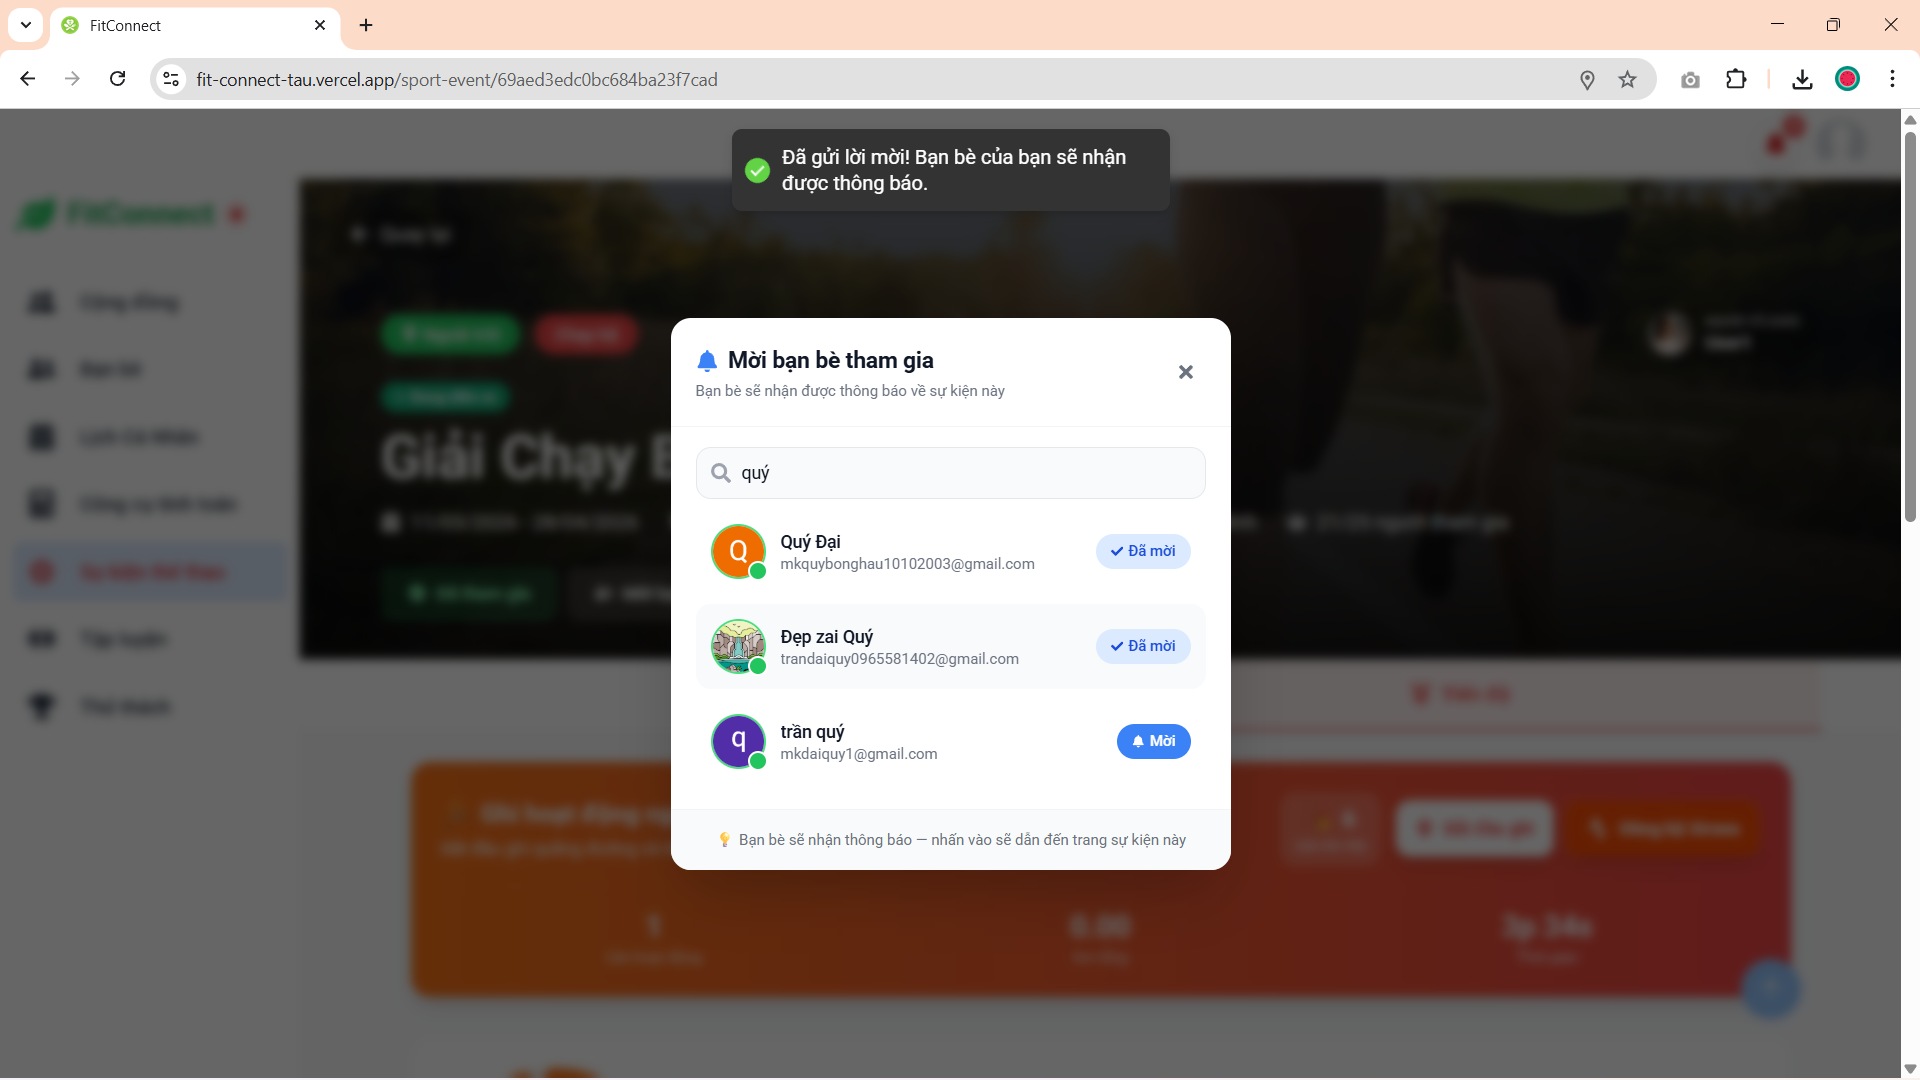
\includegraphics[width=\textwidth]{Images/IMG/nhom3/modalmoimoinguoithamgia.png}
        \caption{Người tham gia thao tác mời mọi người tham gia sự kiện}
        \label{fig:impl_se_invite}
    \end{subfigure}
    \hfill
    \begin{subfigure}[b]{0.47\textwidth}
        \centering
        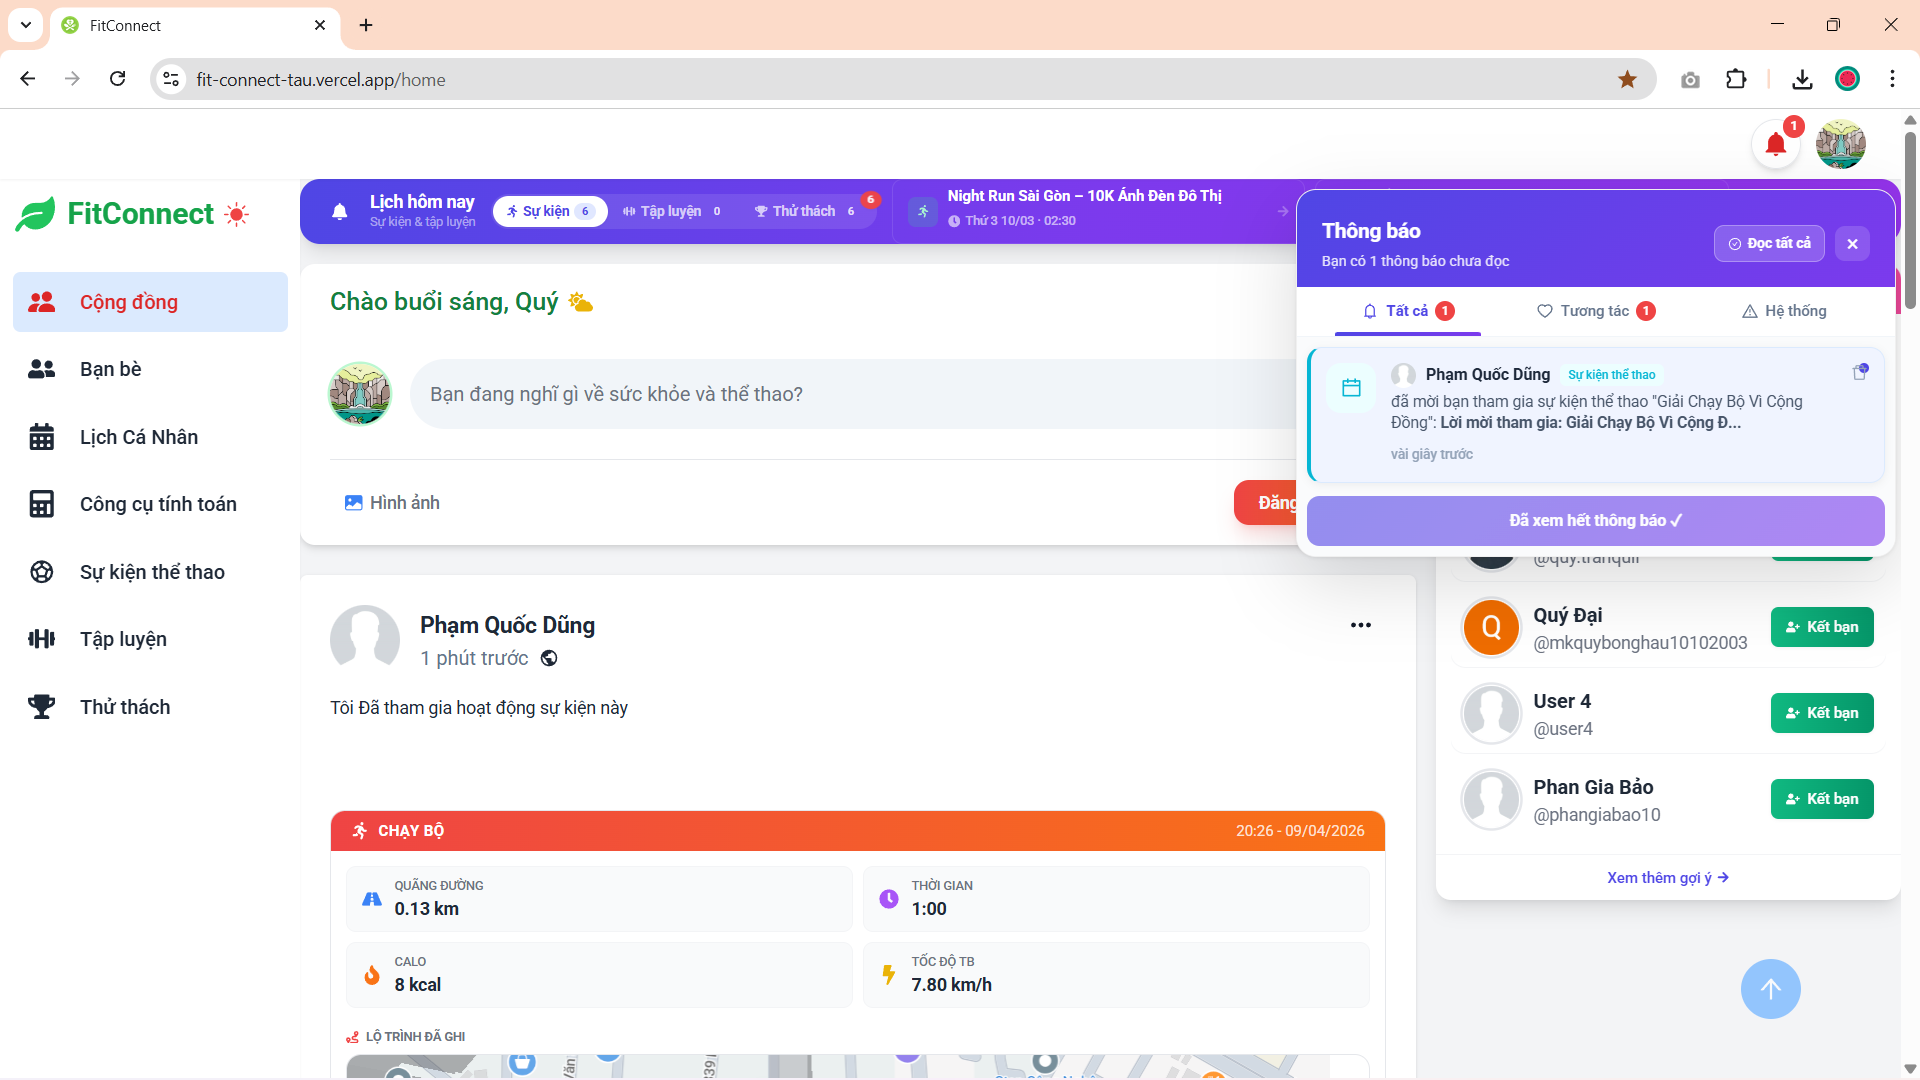
\includegraphics[width=\textwidth]{Images/IMG/nhom3/nguoidcmoithaythongbaomoisk.png}
        \caption{Người được mời nhận thông báo mời tham gia sự kiện}
        \label{fig:impl_se_invite_noti}
    \end{subfigure}
\end{figure}


    \item Người tham gia có thể báo cáo sự kiện vi phạm lên Quản trị viên.

\begin{figure}[H]
    \centering
    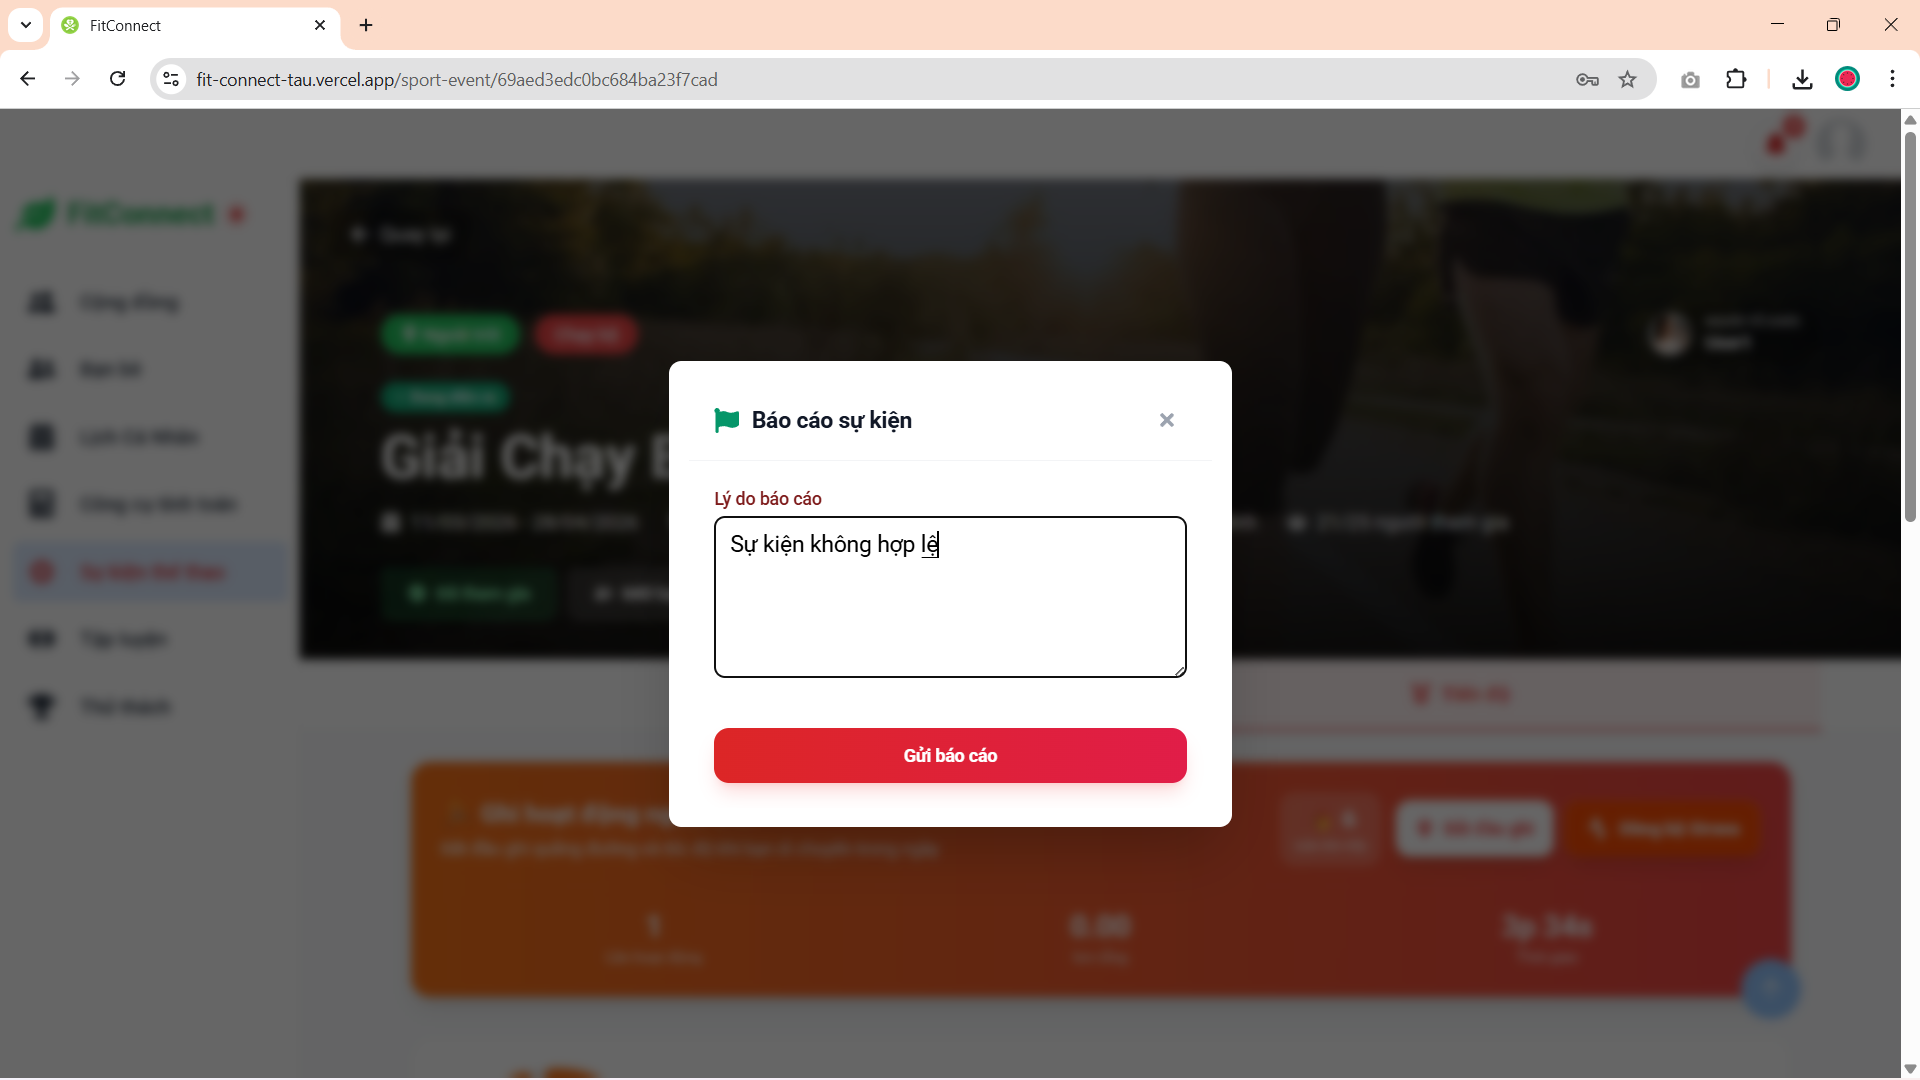
\includegraphics[width=0.60\textwidth]{Images/IMG/nhom3/baocaosukien.png}
    \caption{Người tham gia thao tác báo cáo sự kiện}
    \label{fig:impl_se_report}
\end{figure}

\end{itemize}

\textbf{Tiến độ sự kiện Ngoài trời:}
\begin{itemize}
    \item Đối với sự kiện Ngoài trời, người tham gia có thể nhấn vào tab Tiến độ và xem được thông tin tiến độ tổng quan bao gồm: phần trăm hoàn thành mục tiêu cá nhân, tiến độ đạt được (km), thống kê chi tiết (quãng đường, calories, lần hoạt động, vận tốc trung bình), biểu đồ lịch sử hoạt động và danh sách các hoạt động gần đây.

\begin{figure}[H]
    \centering
    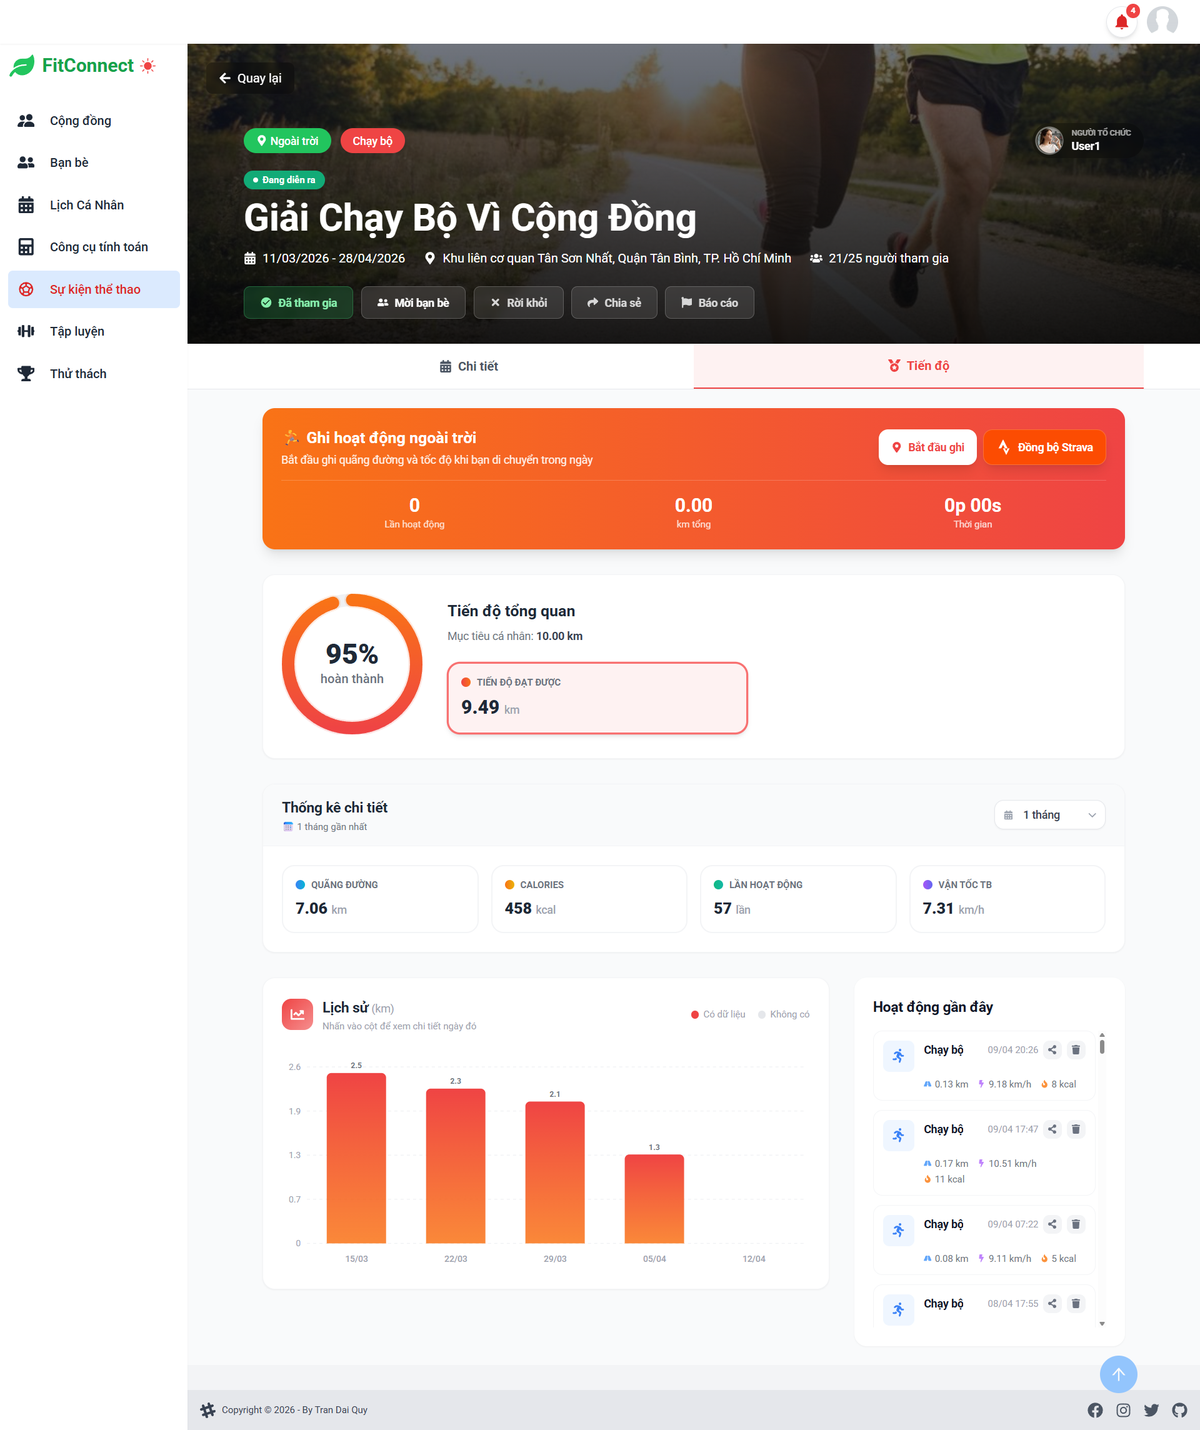
\includegraphics[width=0.60\textwidth]{Images/IMG/nhom3/trangtiendosukien.png}
    \caption{Người tham gia xem trang tiến độ sự kiện ngoài trời}
    \label{fig:impl_se_progress_outdoor}
\end{figure}


    \item Người tham gia có thể ghi tiến độ dựa trên GPS Tracking.
    \begin{itemize}
        \item Khi người tham gia nhấn Bắt đầu ghi (GPS Tracking), hệ thống sẽ hiển thị trang bản đồ với vị trí hiện tại, quãng đường đã đi (km), thời gian, tốc độ (km/h), calories đã đốt (kcal) và thanh tiến độ mục tiêu.

\begin{figure}[H]
    \centering
    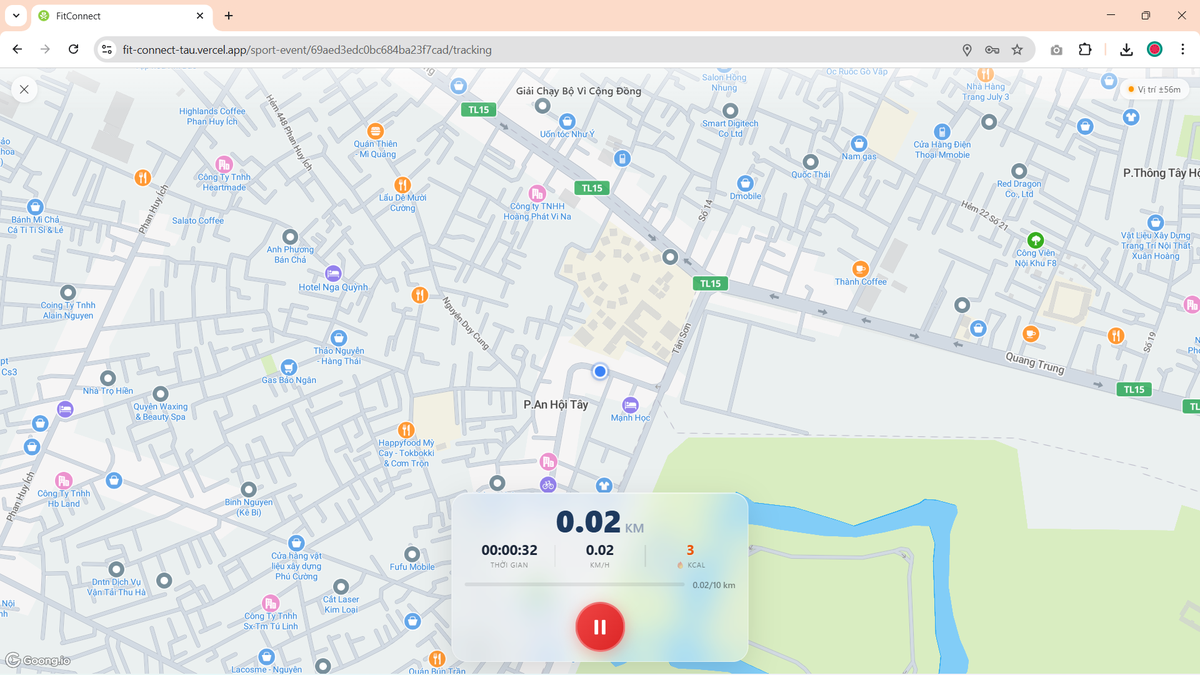
\includegraphics[width=0.60\textwidth]{Images/IMG/nhom3/trackinggpssukienngoaitroi.png}
    \caption{Người tham gia ghi tiến độ bằng GPS tracking sự kiện ngoài trời}
    \label{fig:impl_se_gps}
\end{figure}


        \item Người tham gia nhấn hoàn thành, hệ thống tổng hợp và hiển thị kết quả hoạt động vừa ghi: quãng đường (km), thời gian hoạt động và calories (kcal), đồng thời tự động cập nhật tiến độ sự kiện.


        \item Sau khi hoạt động được lưu, người tham gia có thể nhấn vào từng bản ghi trong danh sách ``Hoạt động gần đây'' để xem chi tiết. Hệ thống hiển thị modal chi tiết hoạt động ngoài trời gồm: loại hoạt động, thời điểm ghi nhận, quãng đường, thời gian, calories, vận tốc trung bình/tối đa và bản đồ lộ trình GPS đã ghi.

\begin{figure}[H]
    \centering
    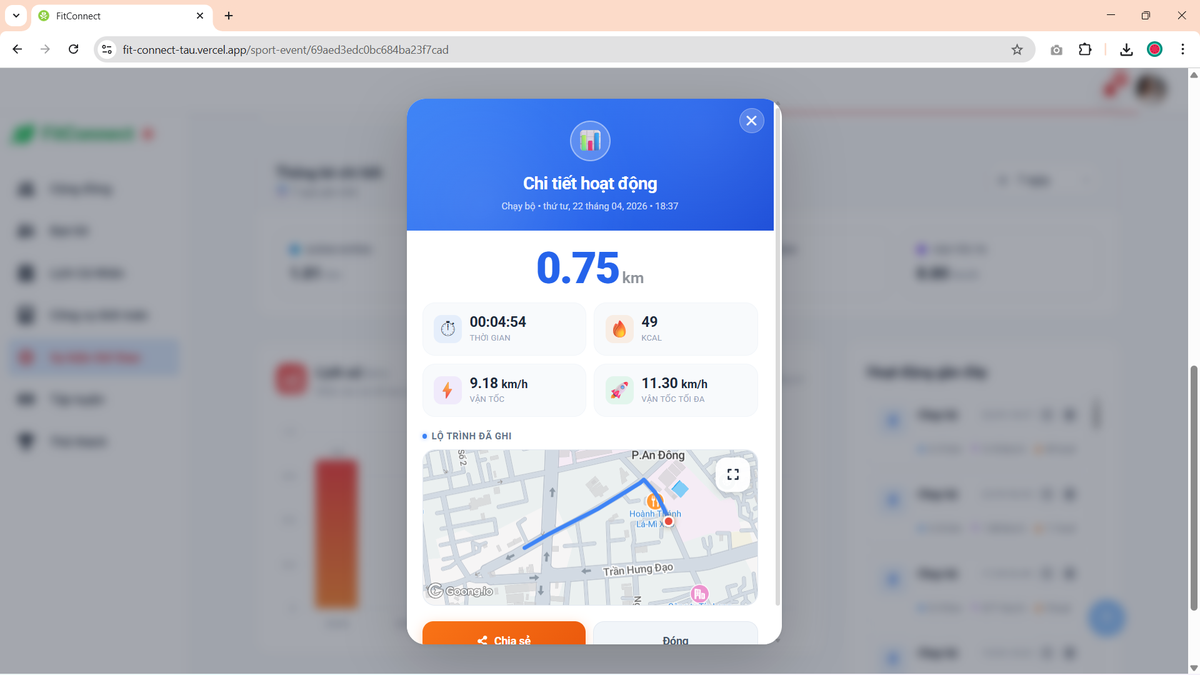
\includegraphics[width=0.60\textwidth]{Images/IMG/nhom3/xemhoatdongsukienngoaitroi.png}
    \caption{Người tham gia xem chi tiết hoạt động sự kiện ngoài trời đã ghi nhận}
    \label{fig:impl_se_view_activity_outdoor}
\end{figure}


        \item Người tham gia có thể chia sẻ hoạt động, sau khi chia sẻ hoạt động sẽ được hiển thị trên bài viết cộng đồng.

\begin{figure}[H]
    \centering
    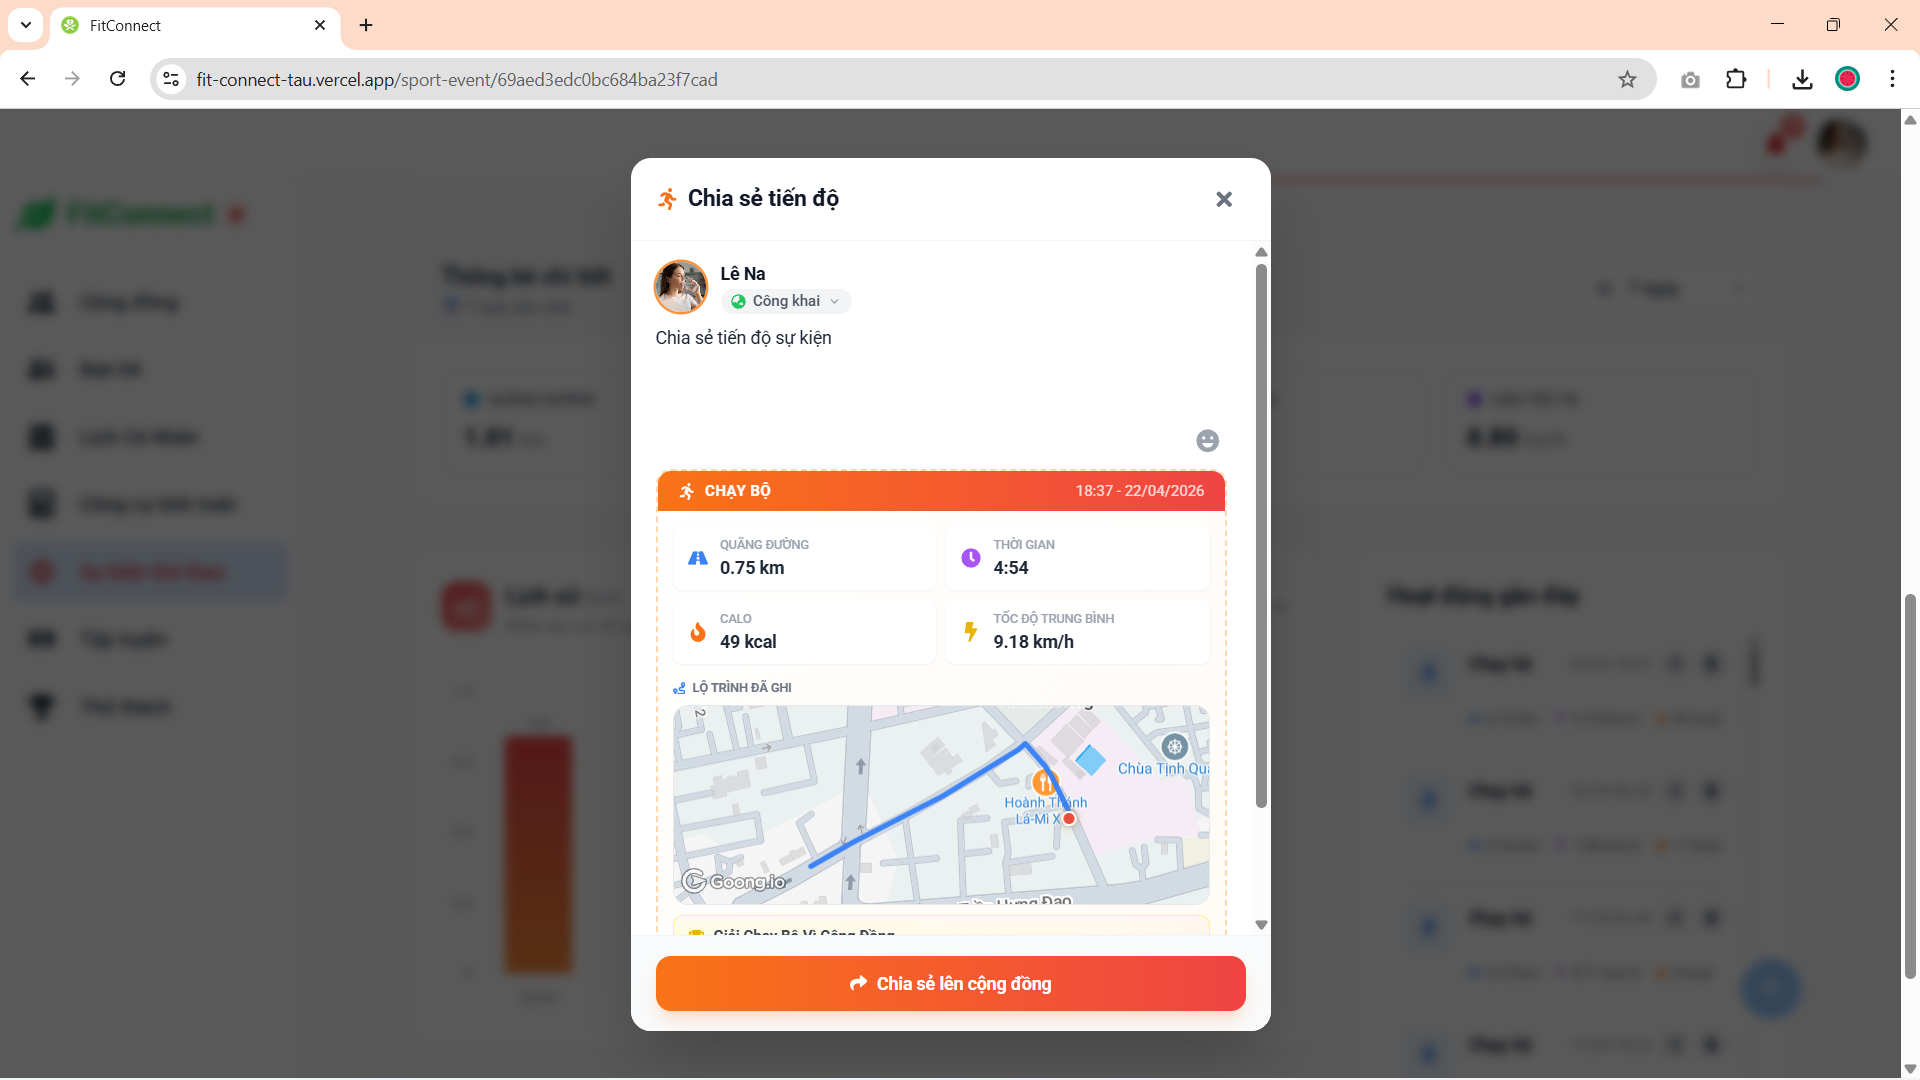
\includegraphics[width=0.60\textwidth]{Images/IMG/nhom3/chiasehoatdongngoaitroi.png}
    \caption{Người tham gia chia sẻ hoạt động ngoài trời lên bảng tin cộng đồng}
    \label{fig:impl_se_share_activity}
\end{figure}


    \end{itemize}
\end{itemize}

\textbf{Tiến độ sự kiện Trong nhà:}
\begin{itemize}
    \item Đối với sự kiện Trong nhà, người tham gia có thể nhấn vào tab Tiến độ và xem được thông tin tiến độ tổng quan bao gồm: phần trăm hoàn thành mục tiêu cá nhân (kcal), tiến độ đạt được, thống kê chi tiết (thời gian, calories, lần tham gia, thời gian trung bình/buổi), biểu đồ lịch sử và danh sách lịch sử buổi học.

\begin{figure}[H]
    \centering
    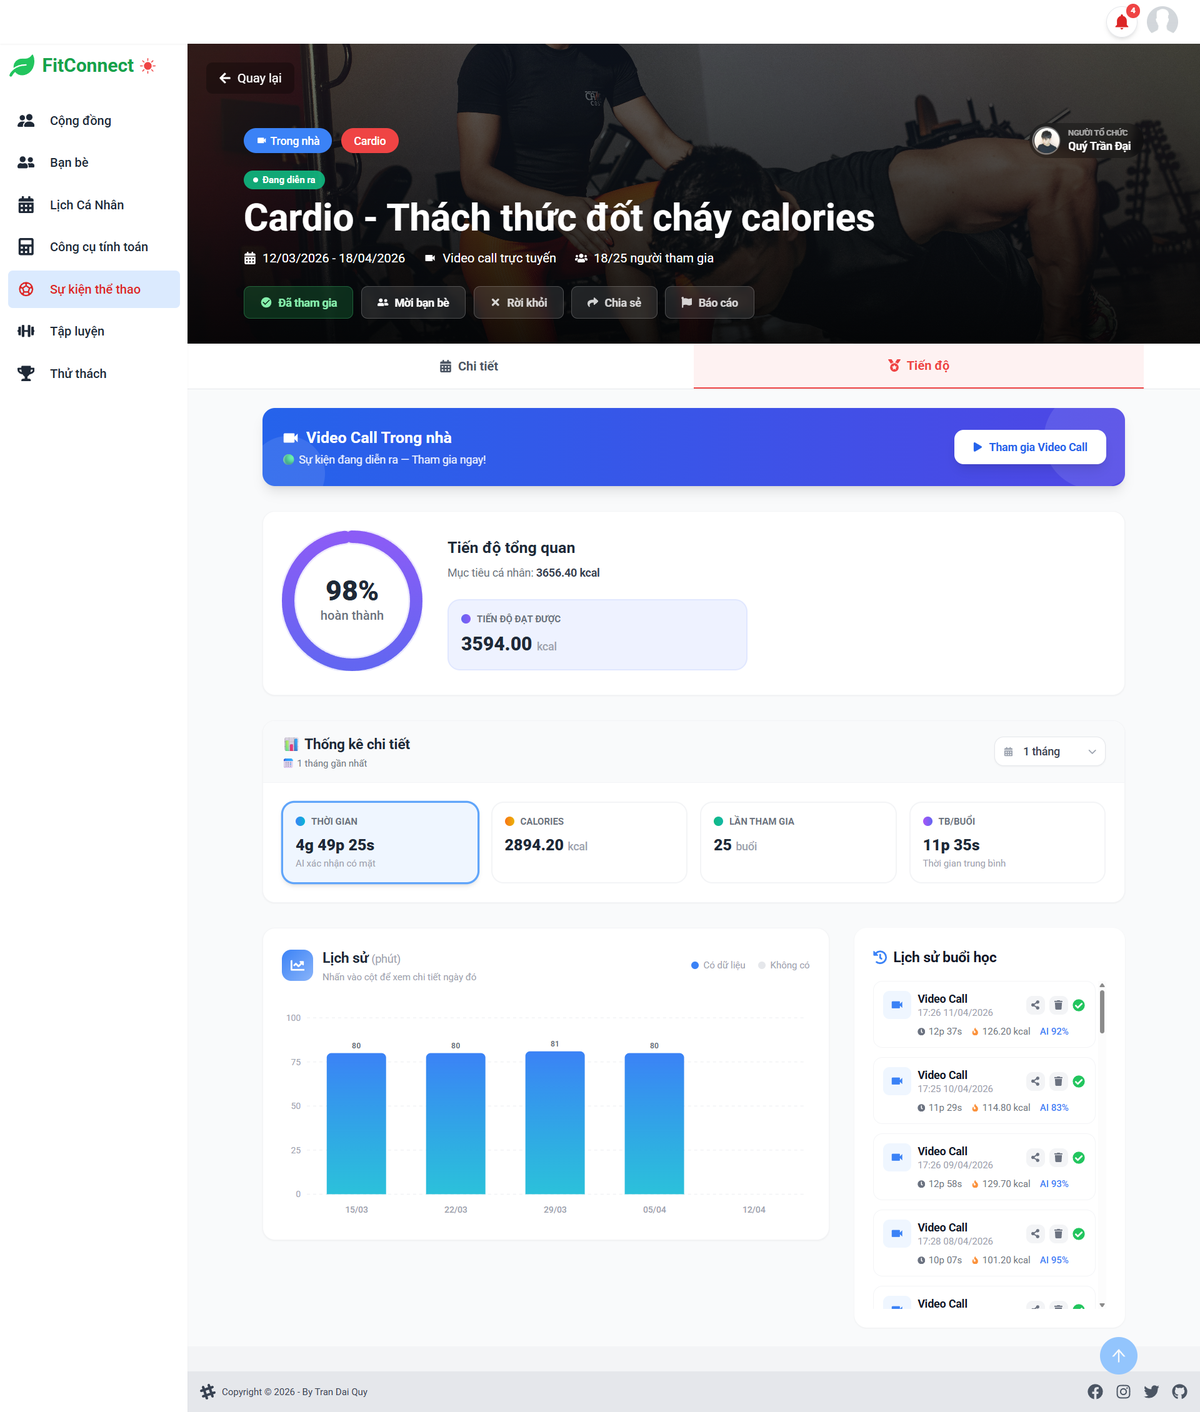
\includegraphics[width=0.60\textwidth]{Images/IMG/nhom3/tiendosukientrongnha.png}
    \caption{Người tham gia xem tiến độ sự kiện trong nhà}
    \label{fig:impl_se_progress_indoor}
\end{figure}


    \item Người tham gia có thể tham gia Video Call sự kiện để tập luyện trực tuyến cùng nhau.
    \begin{itemize}
        \item Khi người tham gia nhấn Tham gia Video Call, hệ thống sẽ hiển thị giao diện video call trực tuyến bao gồm: video của bản thân và các thành viên khác, thời gian tham gia, thời gian thực tế (được AI xác nhận có mặt), calories đã đốt, trạng thái AI đang theo dõi, và các nút chức năng (Tắt mic, Tắt cam, Chia sẻ màn hình, Kết thúc).

\begin{figure}[H]
    \centering
    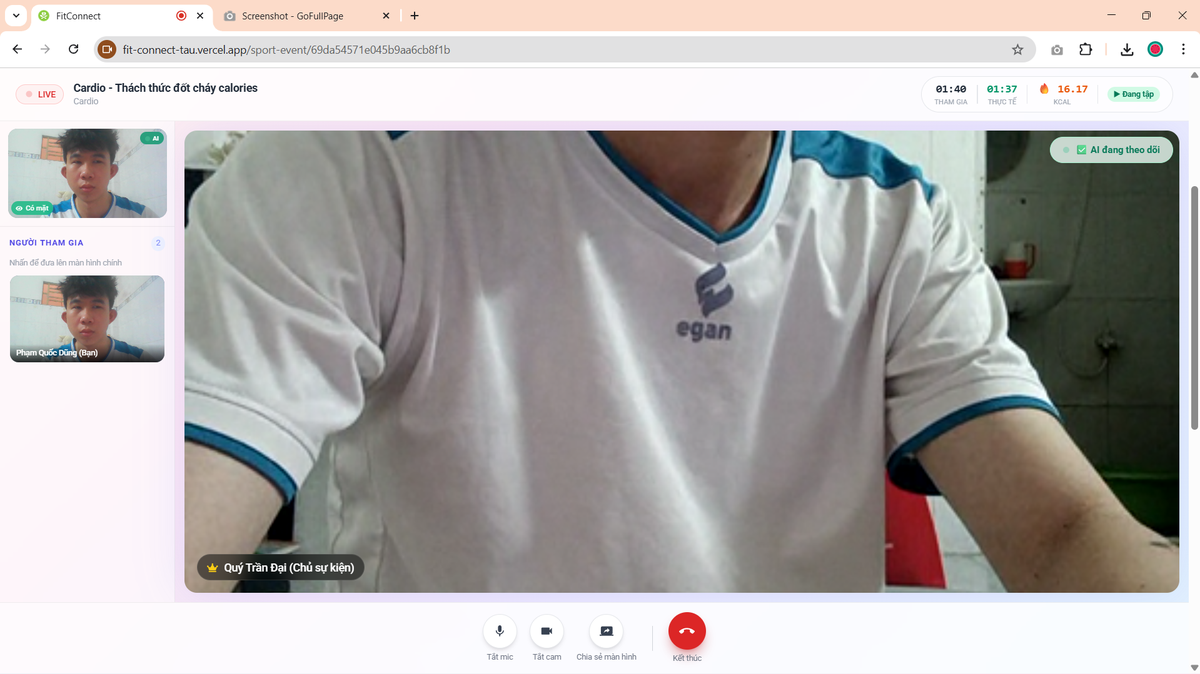
\includegraphics[width=0.60\textwidth]{Images/IMG/nhom3/thamgiavideocall.png}
    \caption{Người tham gia tham gia sự kiện qua Video Call với AI theo dõi}
    \label{fig:impl_se_videocall}
\end{figure}


        \item Nếu người tham gia tắt camera, AI Tracking sẽ nhận diện và tạm dừng ghi nhận thời gian thực tế, đồng thời hiển thị trạng thái ``Vắng'' trên giao diện.

\begin{figure}[H]
    \centering
    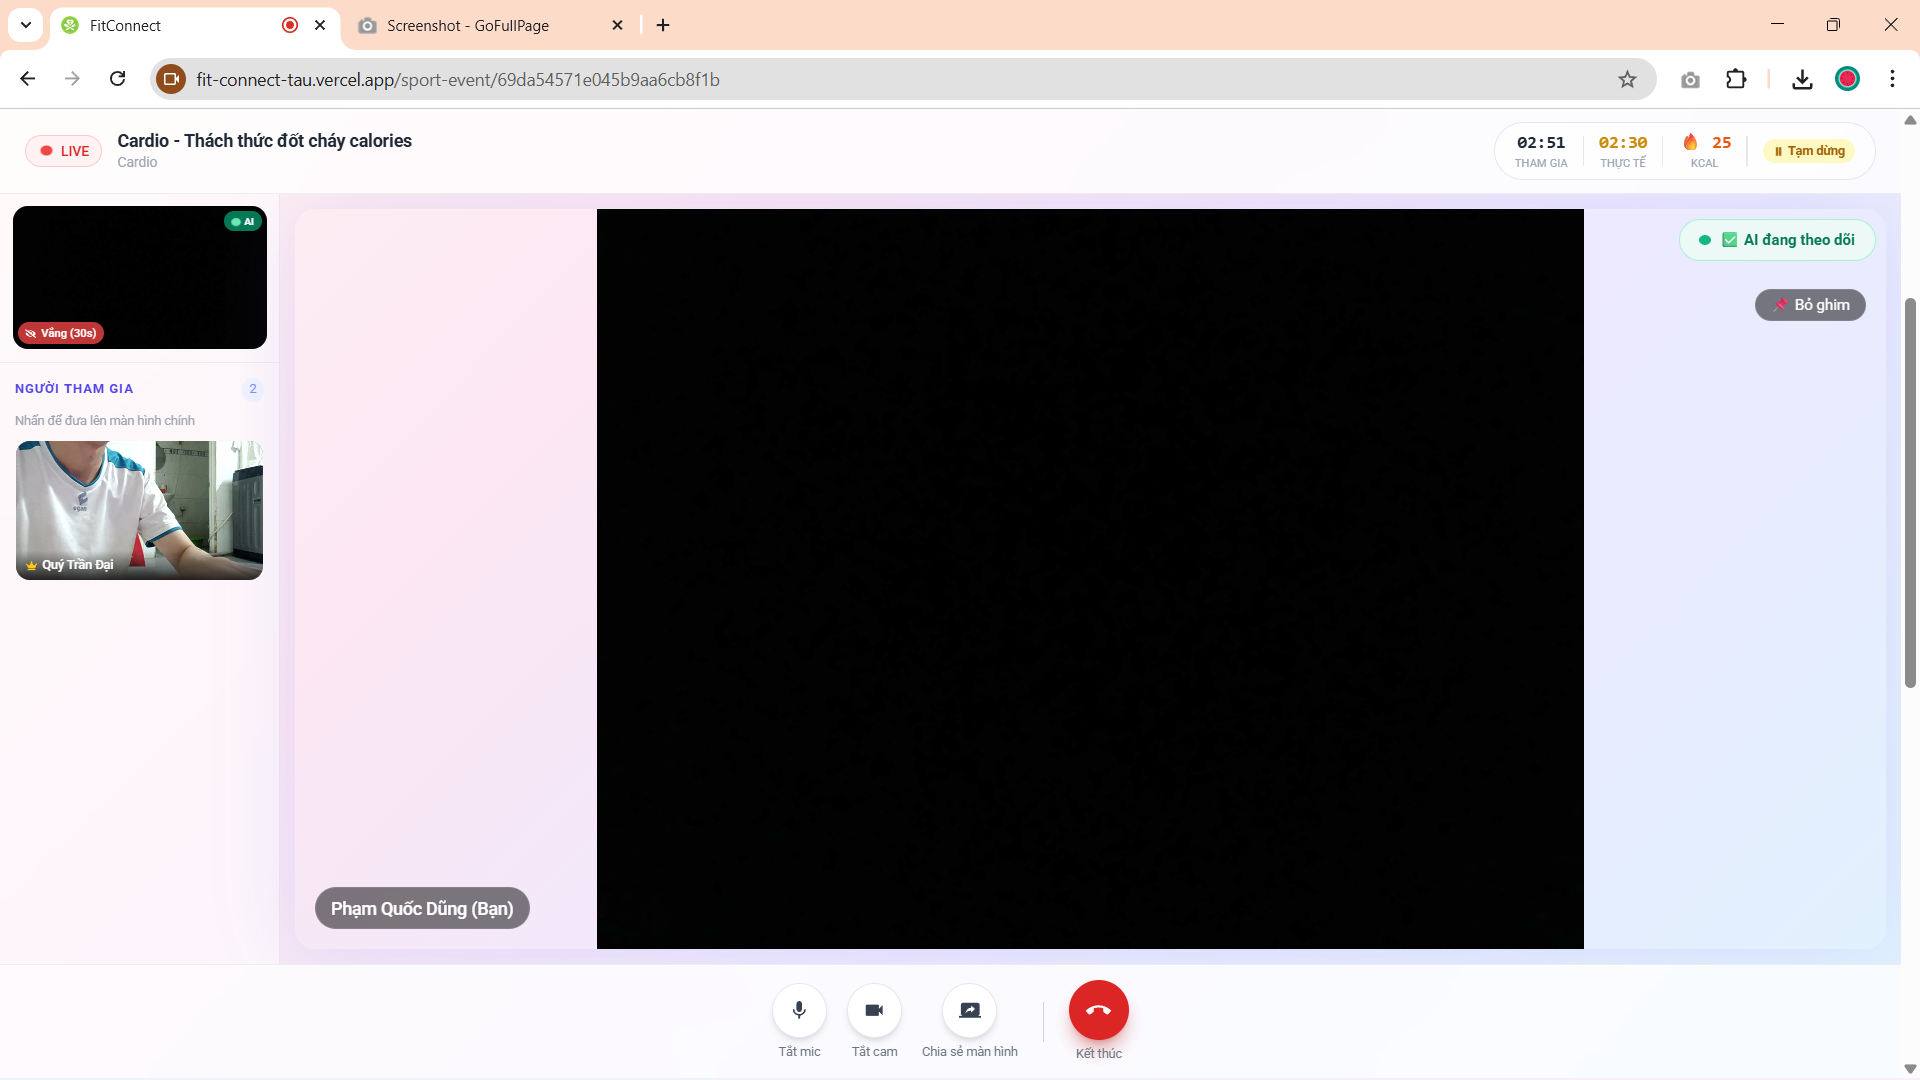
\includegraphics[width=0.60\textwidth]{Images/IMG/nhom3/checameraAInhandientamdung.png}
    \caption{Hệ thống AI nhận diện người tham gia tắt camera và tạm dừng ghi nhận}
    \label{fig:impl_se_ai_pause}
\end{figure}


        \item Sau khi nhấn Kết thúc Video Call, hệ thống tổng hợp thông tin hoạt động: thời gian tham gia, thời gian AI xác nhận có mặt và calories đã đốt (kcal). Người tham gia có thể chia sẻ hoạt động lên bảng tin cộng đồng.

    \end{itemize}
\end{itemize}

\subsubsection{Luồng thao tác quản trị sự kiện (Góc độ Quản trị viên)}
\begin{itemize}
    \item Quản trị viên truy cập trang Kiểm duyệt sự kiện thể thao, hệ thống hiển thị danh sách sự kiện bị báo cáo bao gồm thông tin: người tạo sự kiện, tên sự kiện, số báo cáo, người báo cáo, nội dung báo cáo và các hành động (xem chi tiết, giữ sự kiện, gỡ sự kiện).

\begin{figure}[H]
    \centering
    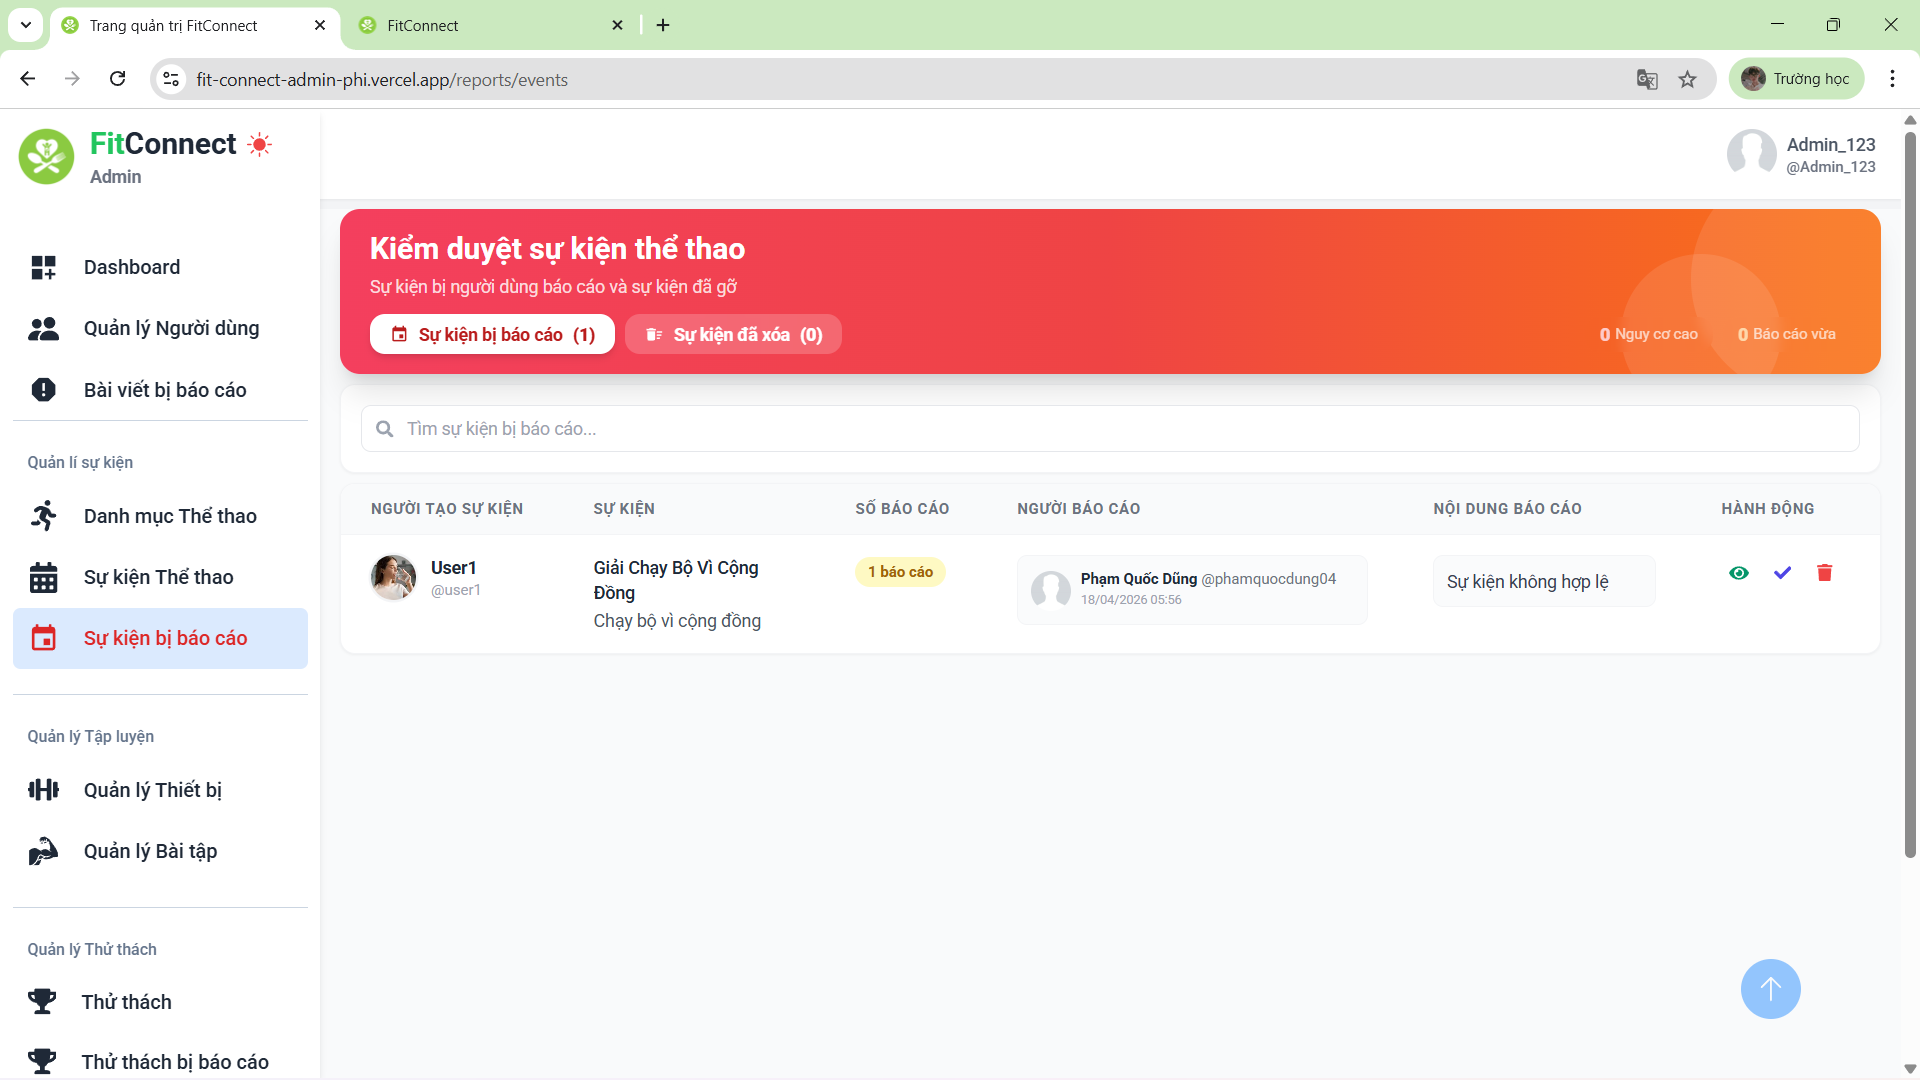
\includegraphics[width=0.60\textwidth]{Images/IMG/nhom3/adminxemdanhsachsukienbaocao.png}
    \caption{Quản trị viên xem danh sách sự kiện bị báo cáo}
    \label{fig:impl_se_admin_list}
\end{figure}


    \item Quản trị viên có thể nhấn xem chi tiết để xem thông tin sự kiện bị báo cáo bao gồm: tên sự kiện, trạng thái, thời gian diễn ra, số người tham gia, danh sách người báo cáo, thông tin sự kiện (thể loại, loại sự kiện, số người tối đa, địa điểm chi tiết).

\begin{figure}[H]
    \centering
    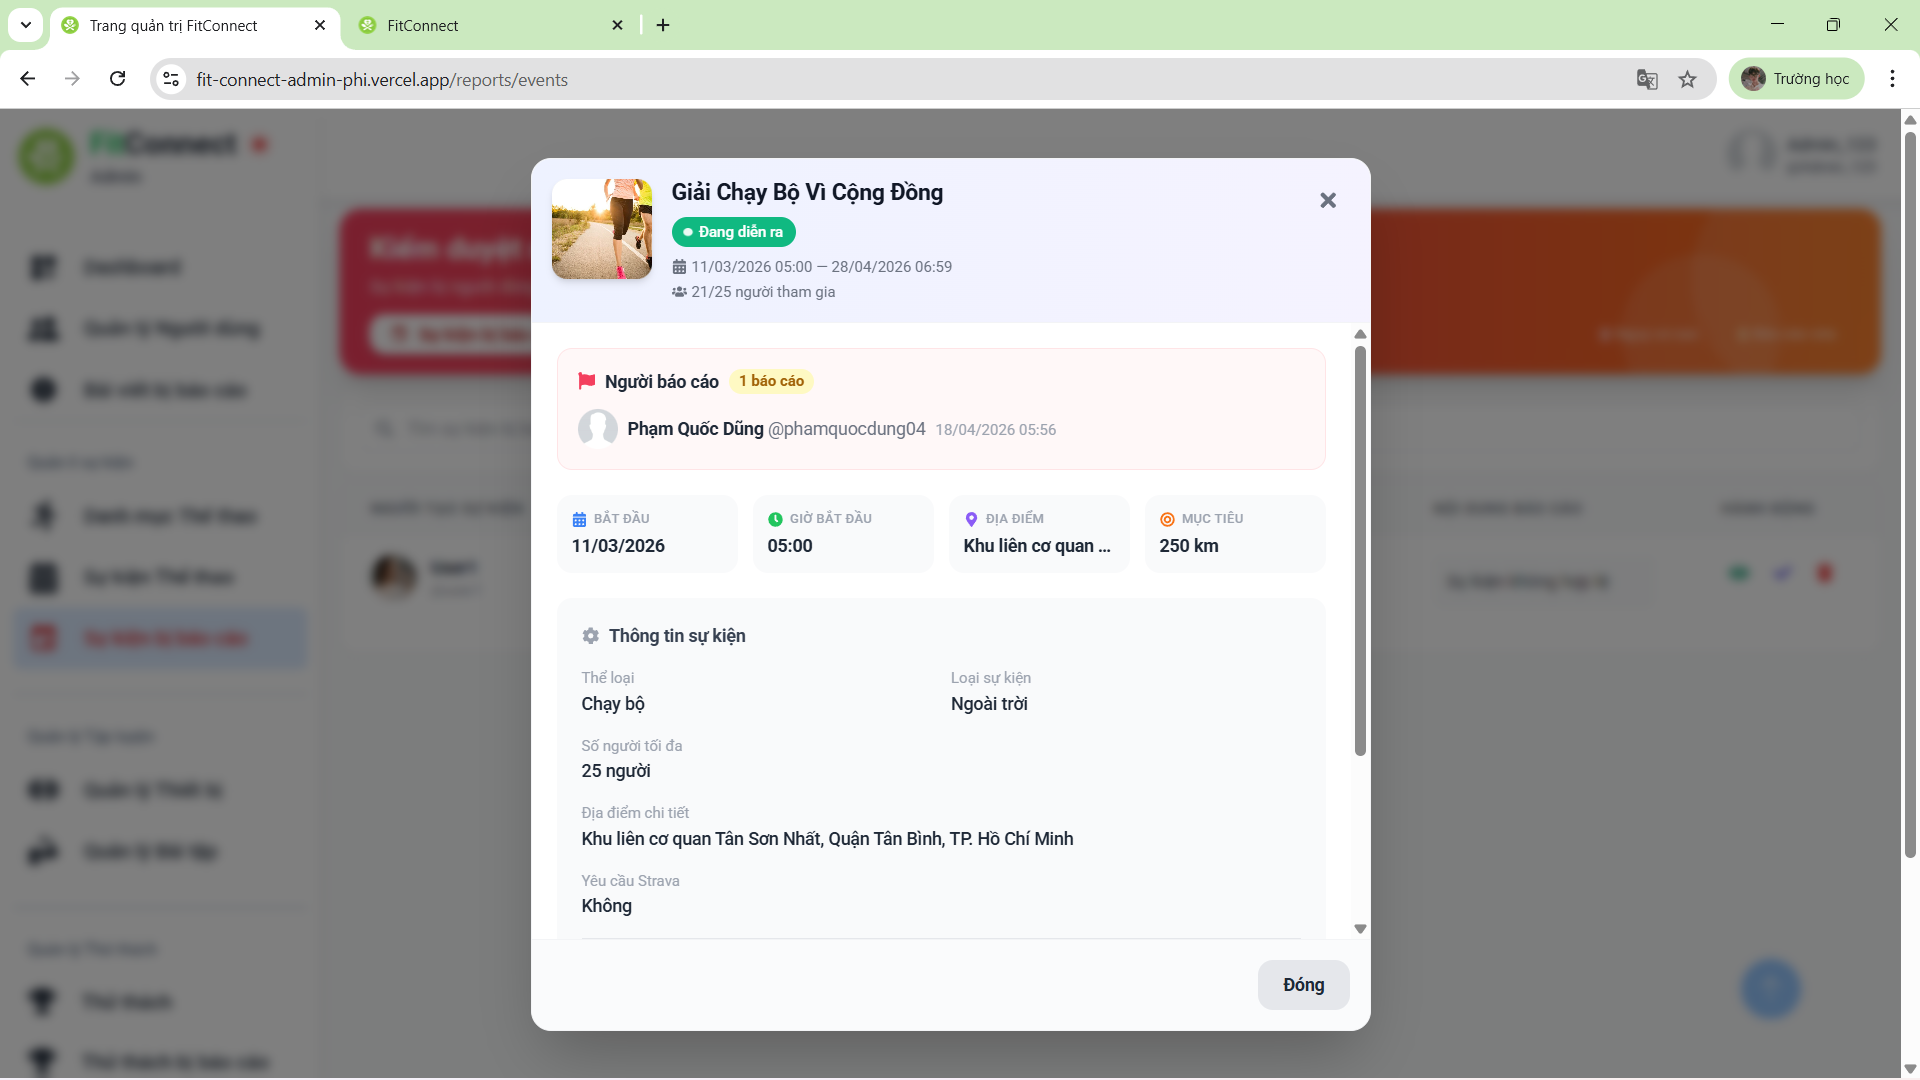
\includegraphics[width=0.60\textwidth]{Images/IMG/nhom3/adminxemthongtinsukienbibaoca.png}
    \caption{Quản trị viên xem thông tin chi tiết sự kiện bị báo cáo}
    \label{fig:impl_se_admin_view}
\end{figure}


    \item Dựa trên xác minh, Admin \textbf{Giữ sự kiện} (xóa toàn bộ báo cáo, sự kiện tiếp tục hoạt động) hoặc \textbf{Gỡ sự kiện} (ẩn khỏi hệ thống, chuyển sang tab ``Đã xóa''). Sự kiện đã gỡ có thể được khôi phục trở lại bất kỳ lúc nào.

\begin{figure}[H]
    \centering
    \begin{subfigure}[b]{0.47\textwidth}
        \centering
        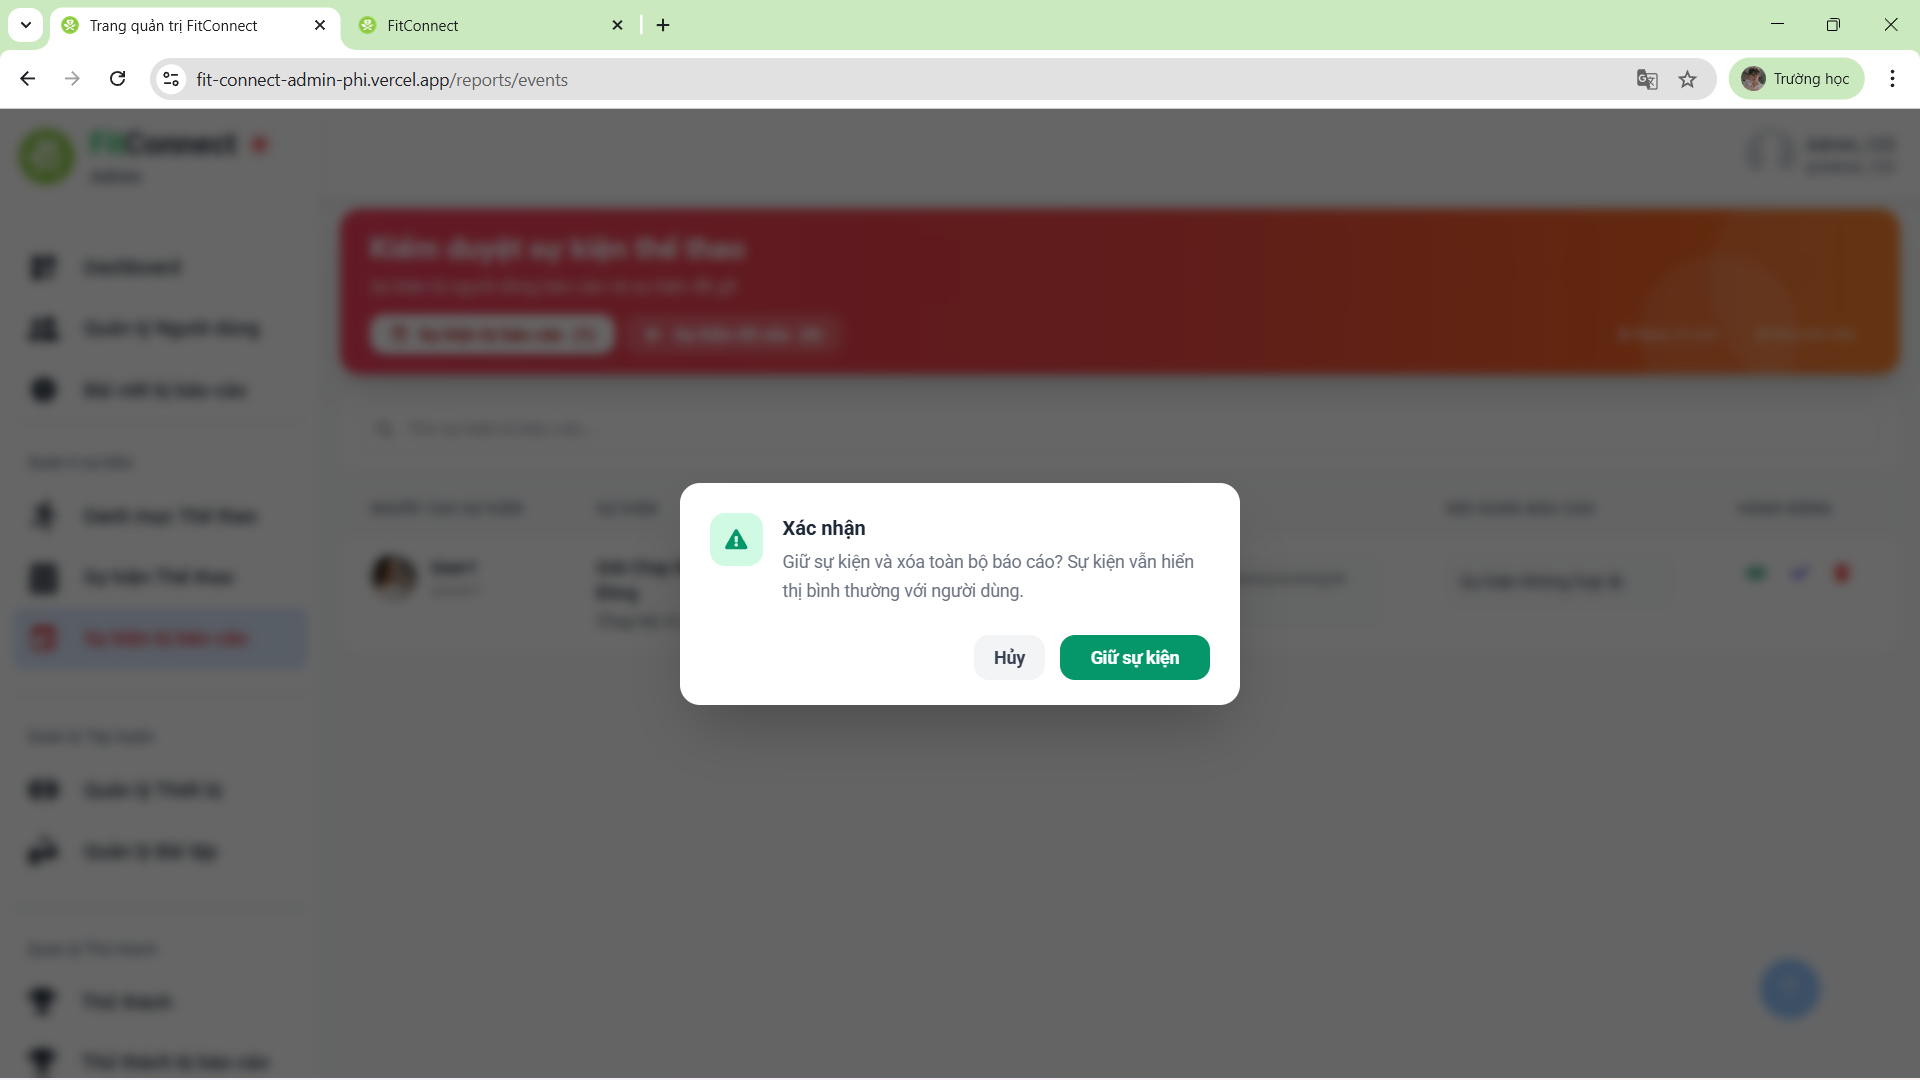
\includegraphics[width=\textwidth]{Images/IMG/nhom3/admingiusukien.png}
        \caption{Xác nhận giữ sự kiện hợp lệ}
        \label{fig:impl_se_admin_keep}
    \end{subfigure}
    \hfill
    \begin{subfigure}[b]{0.47\textwidth}
        \centering
        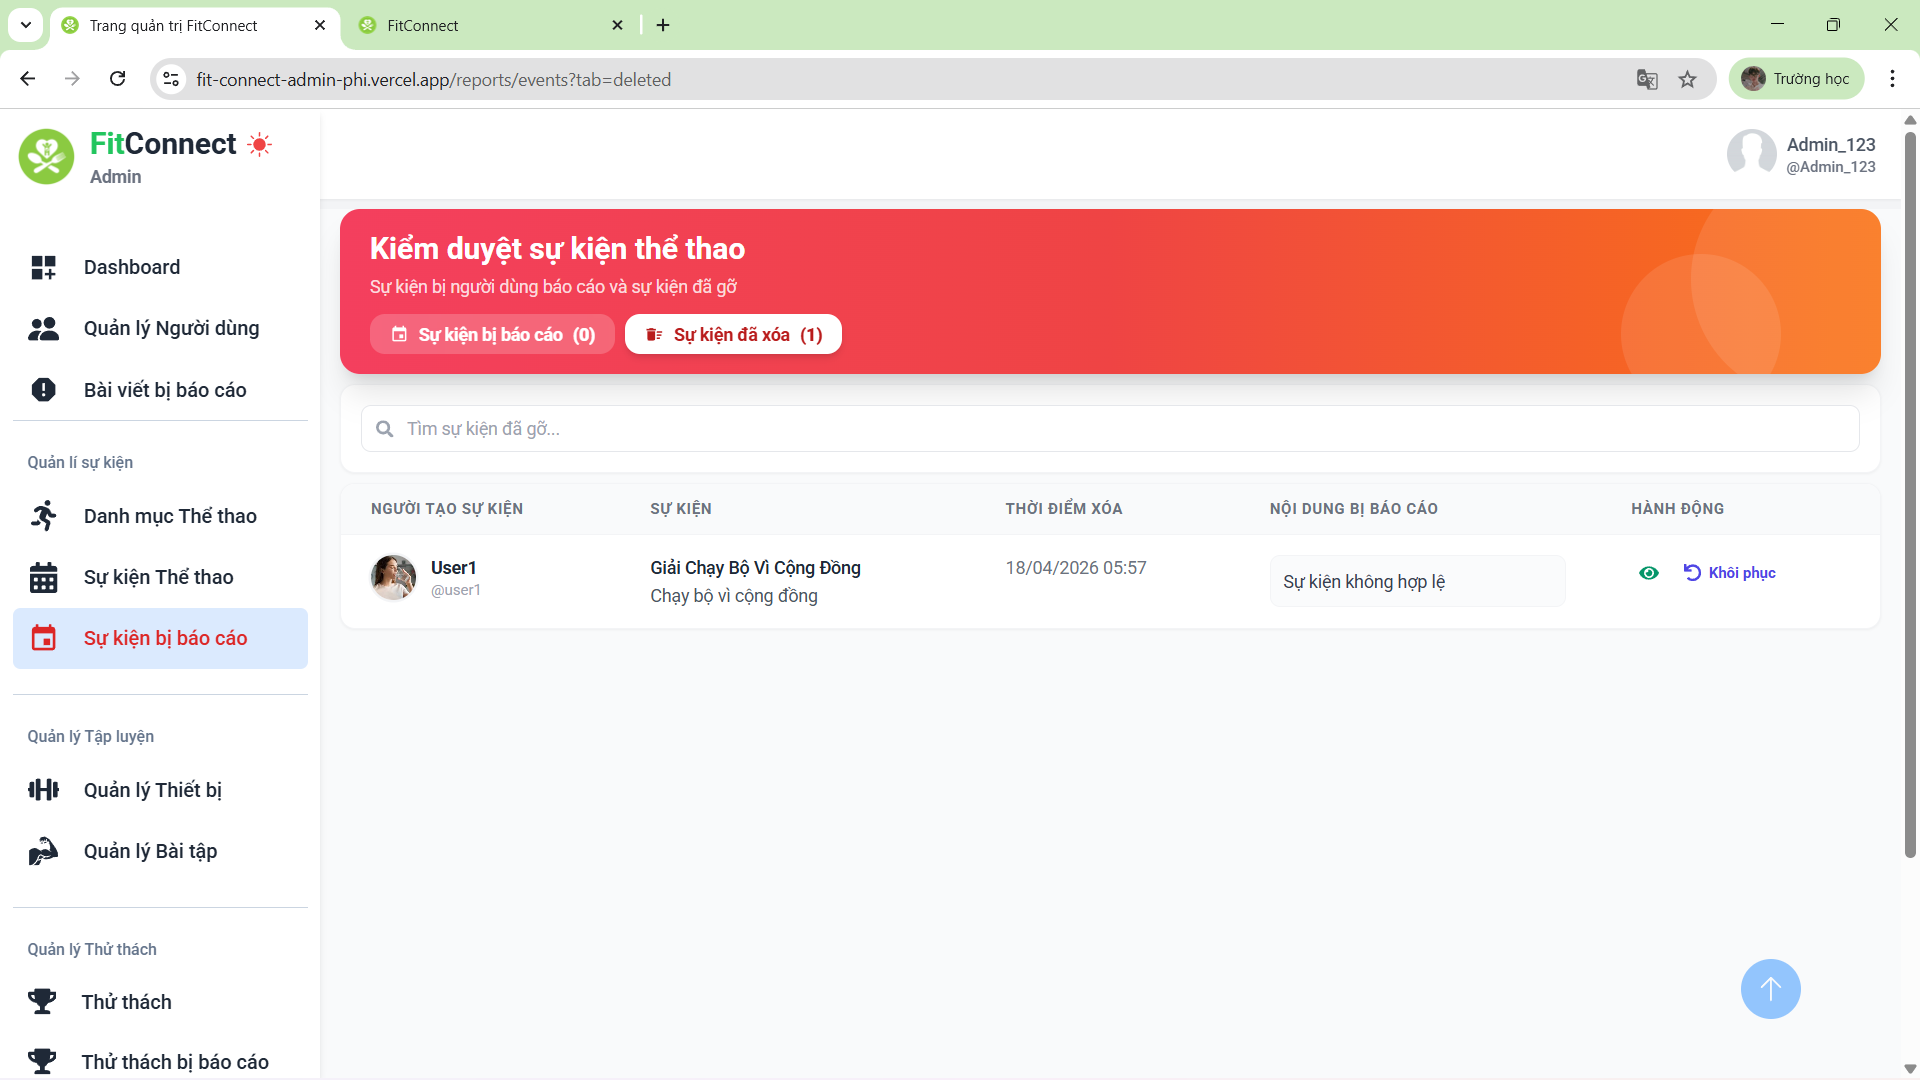
\includegraphics[width=\textwidth]{Images/IMG/nhom3/adminxemsukienbixoa.png}
        \caption{Danh sách sự kiện đã xóa và tùy chọn khôi phục}
        \label{fig:impl_se_admin_deleted_list}
    \end{subfigure}
    \vspace{0.3em}
    \caption{Xử lý kiểm duyệt sự kiện bị báo cáo và quản lý kho sự kiện đã xóa}
    \label{fig:impl_se_admin_moderation}
\end{figure}

\end{itemize}

\subsection{Nhóm tính năng Thử thách cộng đồng}
\label{subsec:impl_challenge}

Nhóm tính năng Thử thách cộng đồng cho phép người dùng tạo và tham gia các thử thách hàng ngày nhằm duy trì thói quen luyện tập và ăn uống lành mạnh. Hệ thống hỗ trợ ba loại thử thách: Ngoài trời (chạy bộ, đạp xe, leo núi,...) với tiến độ ghi nhận qua GPS Tracking, Ăn uống (ăn sạch, giảm cân, detox,...) với tiến độ ghi nhận qua chụp ảnh bữa ăn, và Thể dục (Workout, tập gym,...) với tiến độ ghi nhận qua xác nhận hoàn thành. Mỗi thử thách đặt mục tiêu theo ngày, và người tham gia cần hoàn thành mục tiêu hàng ngày trong suốt thời gian diễn ra thử thách. Ngoài ra, hệ thống còn tích hợp AI để hỗ trợ tạo thử thách tự động qua hai bước đơn giản.

Quy trình hoạt động gồm ba luồng chính:
\begin{itemize}
    \item \textbf{Người dùng (Người tạo thử thách):} Tạo, quản lý thử thách, theo dõi danh sách người tham gia và chỉnh sửa thông tin thử thách.
    \item \textbf{Người dùng (Người tham gia):} Tìm kiếm, tham gia thử thách, ghi tiến độ hàng ngày, chia sẻ và mời bạn bè.
    \item \textbf{Quản trị viên:} Xử lý các thử thách bị báo cáo từ cộng đồng.
\end{itemize}

\subsubsection{Luồng thao tác tạo và quản lý thử thách (Góc độ Người tạo)}
\begin{itemize}
    \item Người dùng truy cập trang Thử thách, hệ thống hiển thị danh sách các thử thách nổi bật dạng banner ở đầu trang, kèm thanh tìm kiếm và bộ lọc theo loại thử thách (Ăn uống, Ngoài trời, Thể dục) và theo danh mục môn thể thao (Cardio, Thiền, Khiêu vũ, Chạy bộ đường dài,...).

\begin{figure}[H]
    \centering
    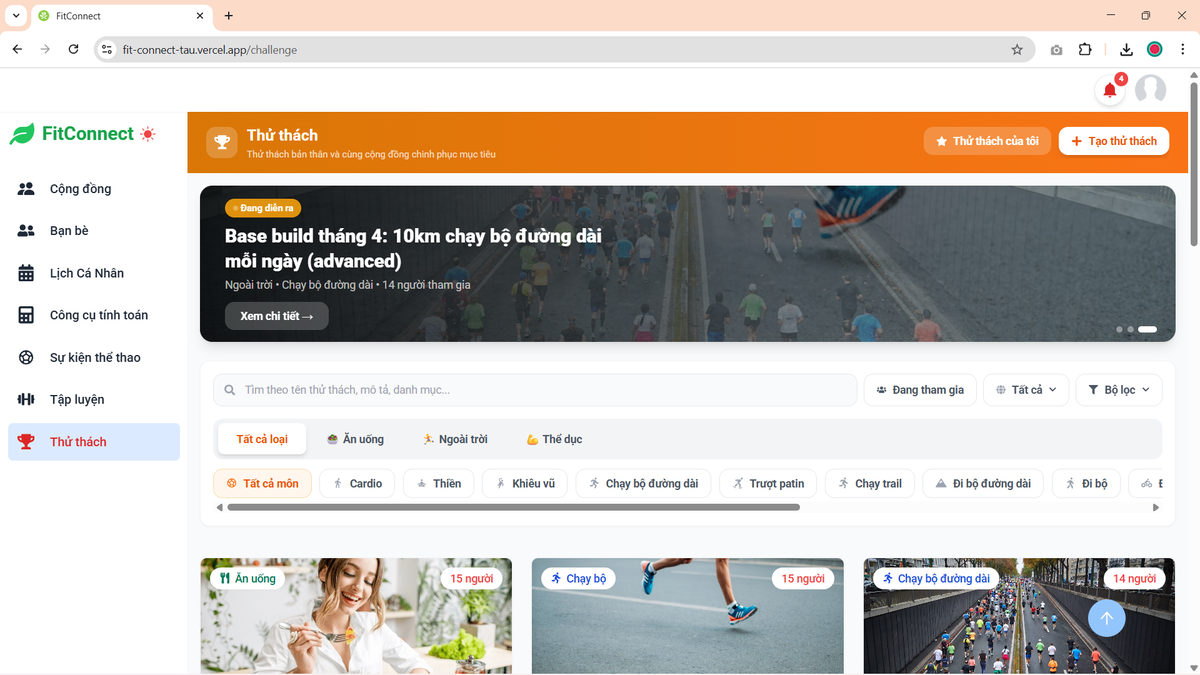
\includegraphics[width=0.60\textwidth]{Images/IMG/nhom4/trangdanhsachthuthach.png}
    \caption{Người dùng xem trang danh sách thử thách cộng đồng}
    \label{fig:impl_ch_list}
\end{figure}


    \item Người dùng nhấn Tạo thử thách mới, hệ thống hiển thị modal tạo thử thách bao gồm các thông tin: loại thử thách (Ngoài trời, Ăn uống, Thể dục), tên thử thách, danh mục hoạt động, mục tiêu mỗi ngày (km hoặc kcal hoặc bữa tùy loại), ngày bắt đầu, ngày kết thúc, hình thức tham gia (Công khai, Bạn bè, Chỉ mình tôi), và hình ảnh. Bên phải có khung Bản xem trước cập nhật real-time khi nhập thông tin.

\begin{figure}[H]
    \centering
    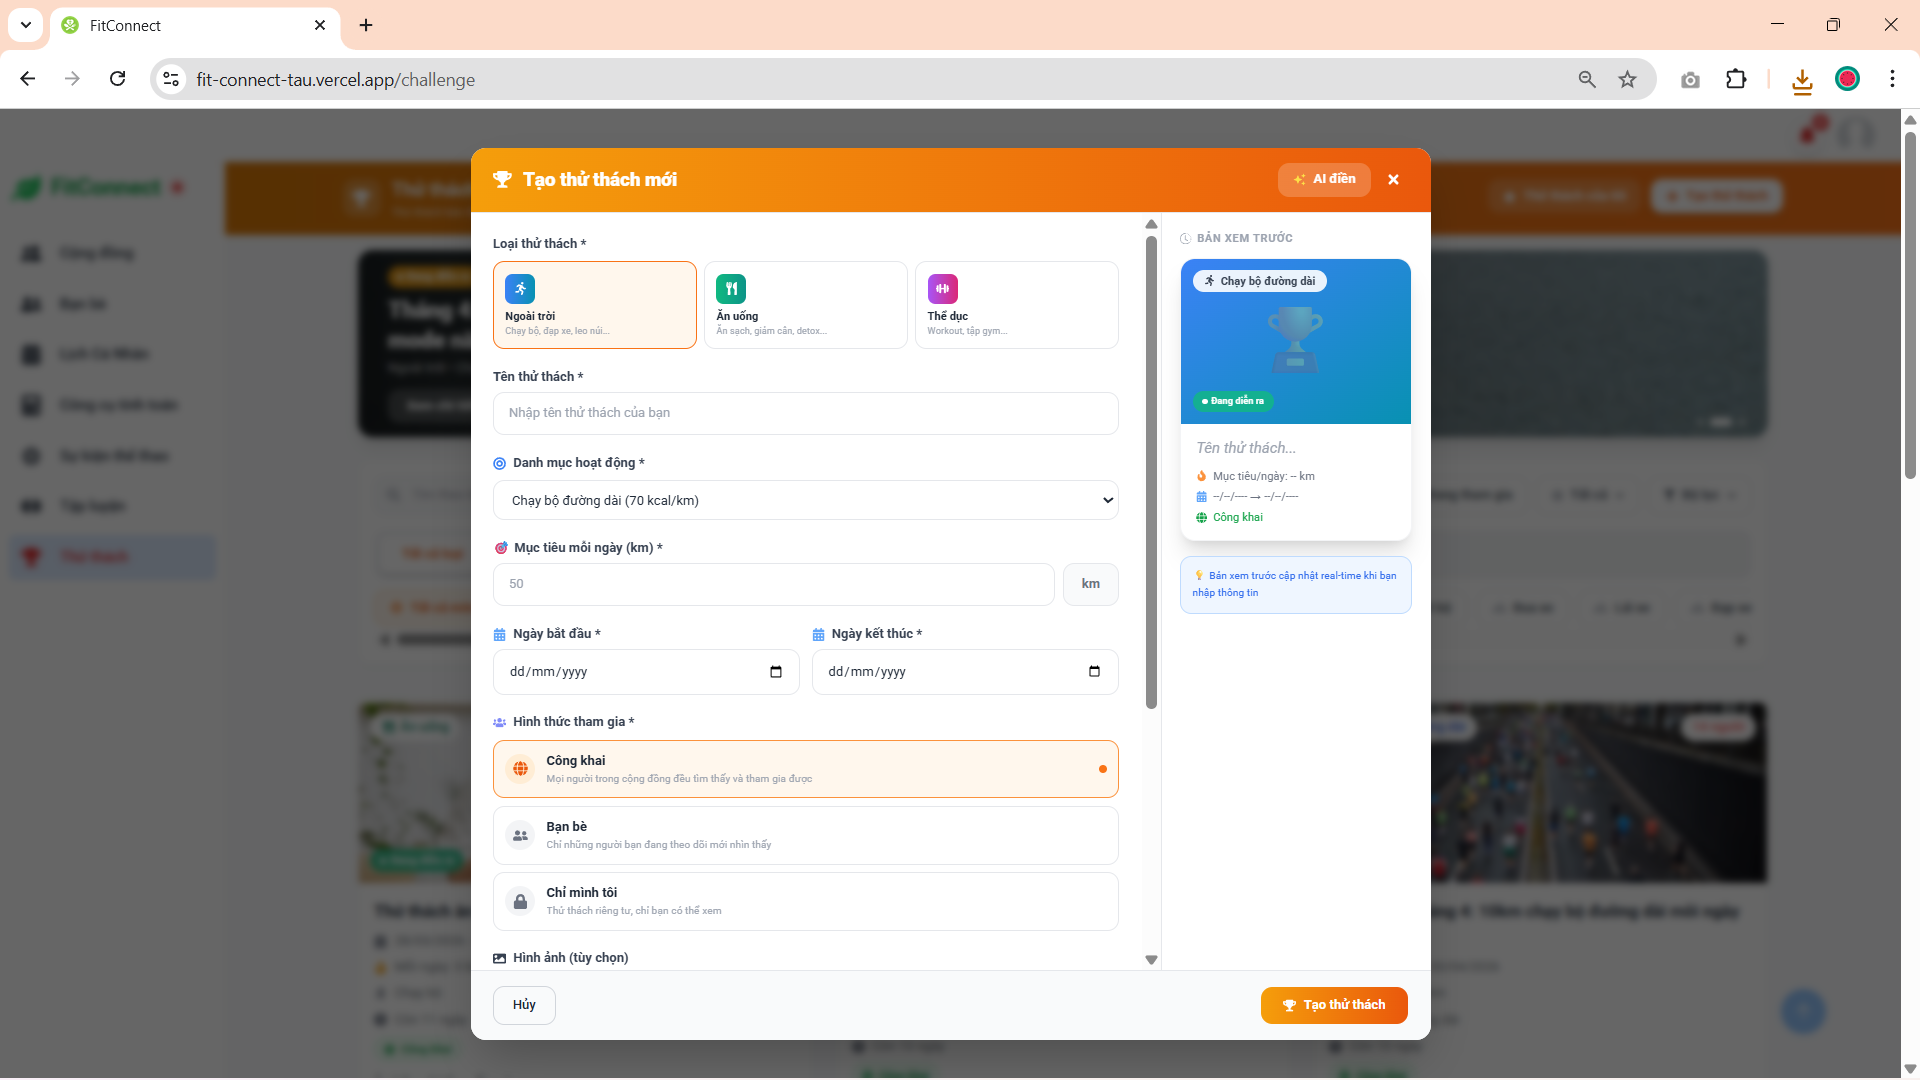
\includegraphics[width=0.60\textwidth]{Images/IMG/nhom4/manhinhtaothuthach.png}
    \caption{Người dùng thao tác tạo thử thách mới}
    \label{fig:impl_ch_create}
\end{figure}


    \item Người dùng có thể dùng tính năng AI tự điền thử thách qua hai bước: Bước 1 -- chọn loại thử thách muốn tạo (Ngoài trời, Ăn uống, Thể dục); Bước 2 -- mô tả ý tưởng thử thách bằng ngôn ngữ tự nhiên (ví dụ: ``Tạo thử thách chạy bộ ngoài trời 1km mỗi ngày từ nay tới hết tháng''), sau đó nhấn Điền ngay để AI tự động điền toàn bộ biểu mẫu.

\begin{figure}[H]
    \centering
    \begin{subfigure}[b]{0.30\textwidth}
        \centering
        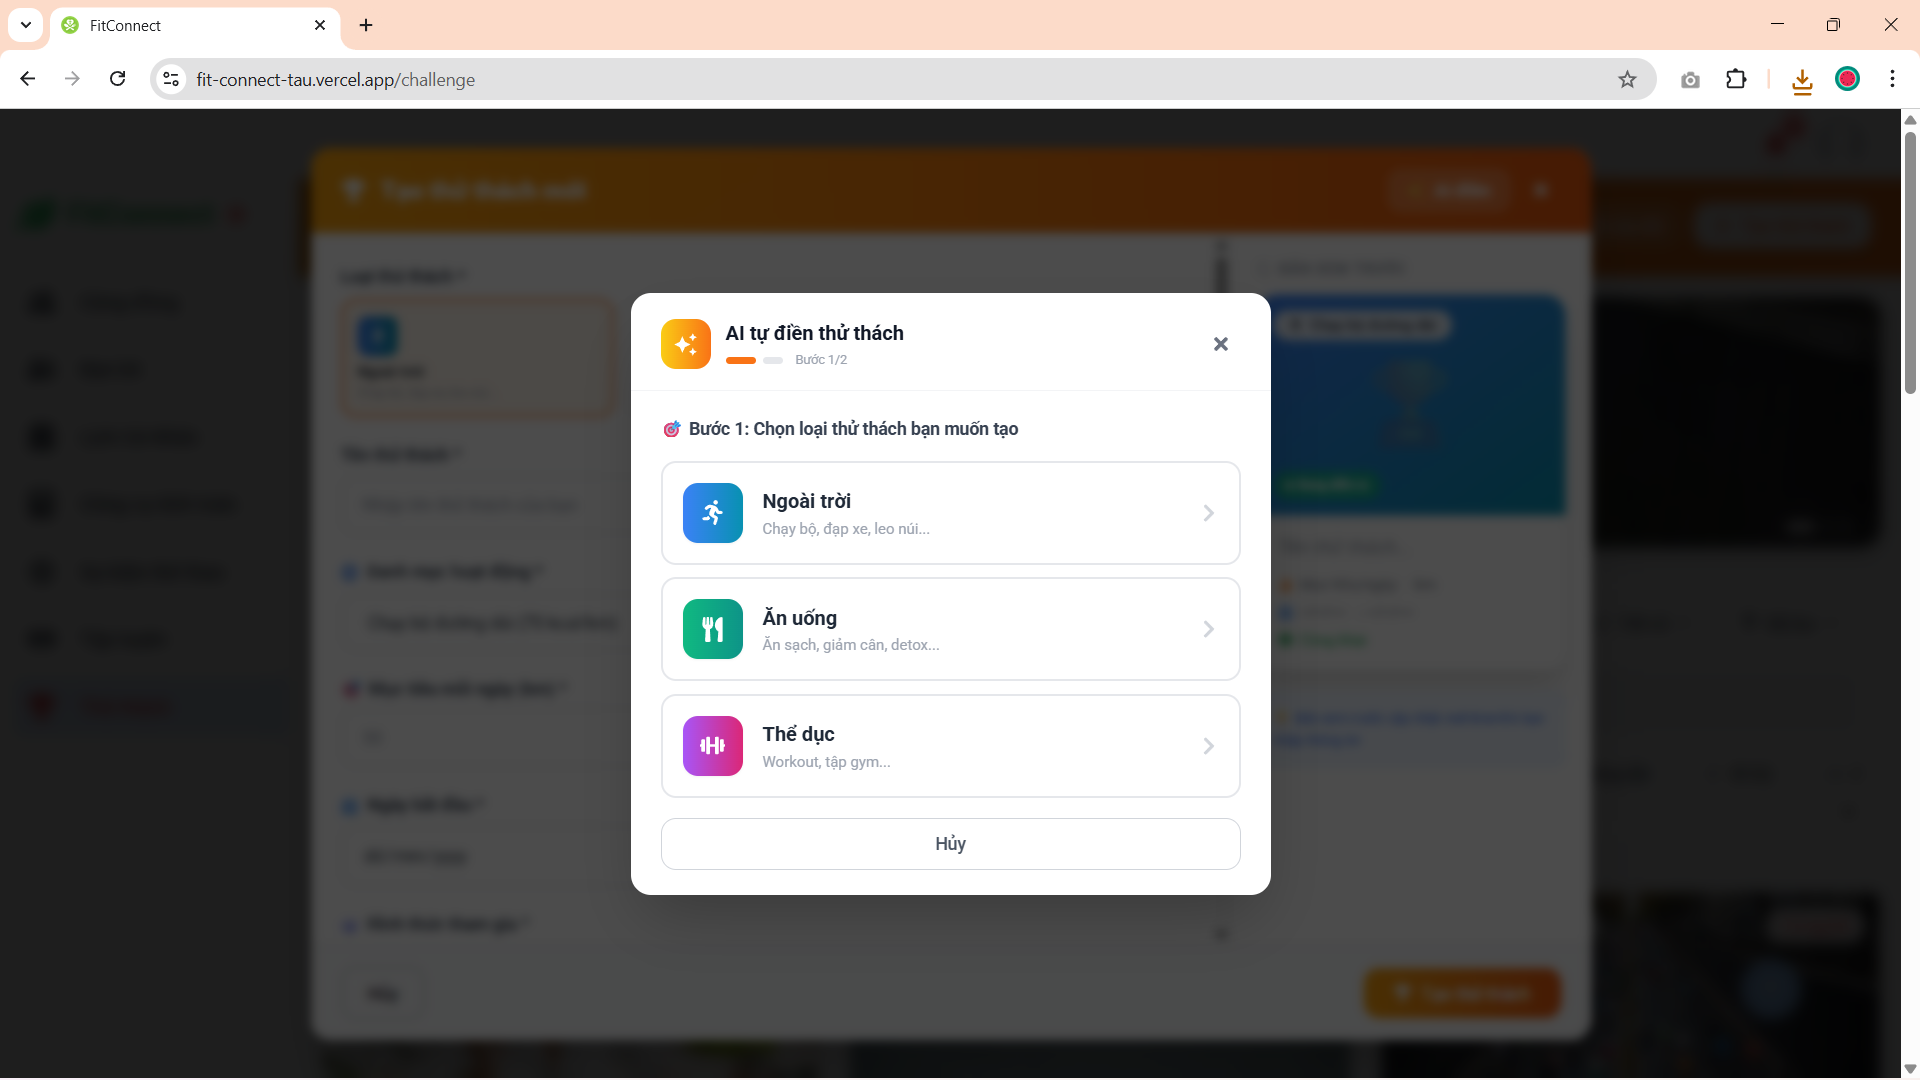
\includegraphics[width=\textwidth]{Images/IMG/nhom4/modalchonloaithuthachtruocAI.png}
        \caption{Hệ thống hiển thị modal AI tự điền thử thách -- Bước 1 chọn loại thử thách}
        \label{fig:impl_ch_ai_step1}
    \end{subfigure}
    \hfill
    \begin{subfigure}[b]{0.30\textwidth}
        \centering
        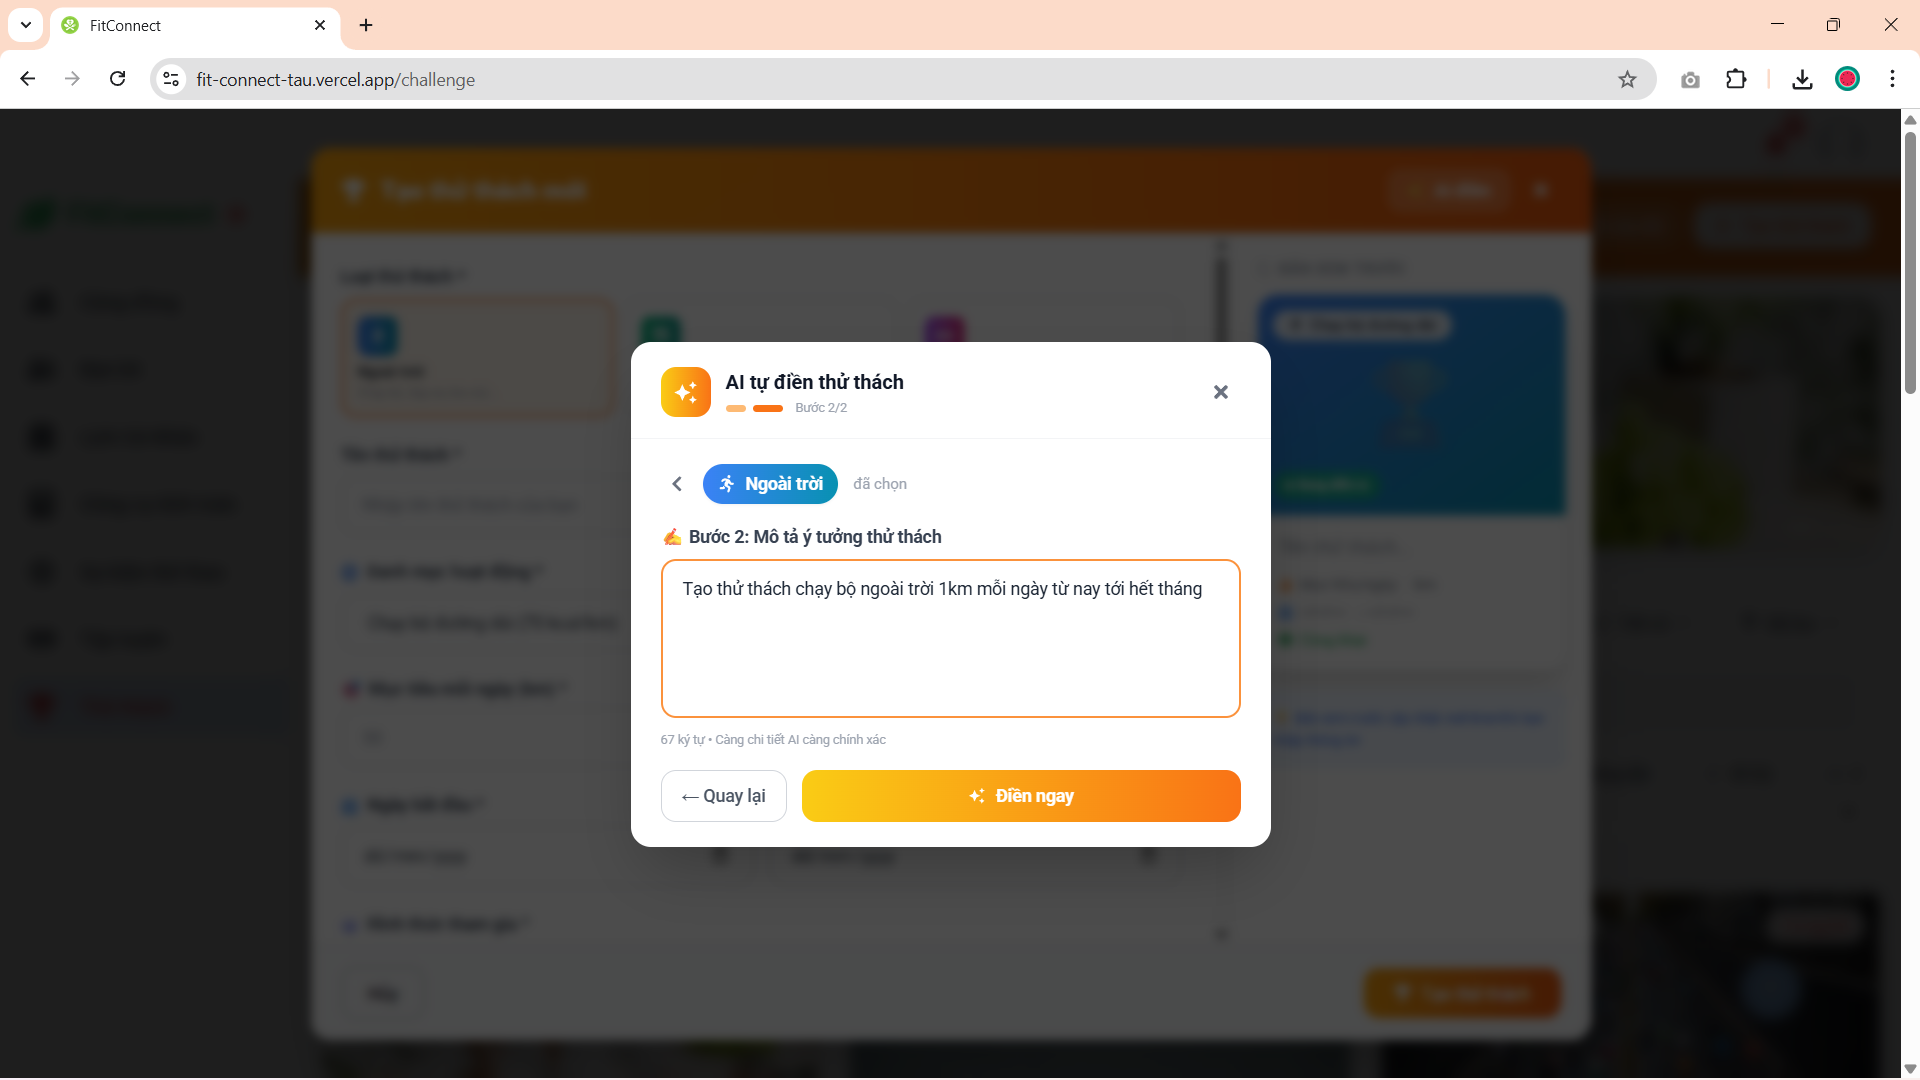
\includegraphics[width=\textwidth]{Images/IMG/nhom4/modalAItaothuthach.png}
        \caption{Hệ thống hiển thị modal AI tự điền thử thách -- Bước 2 mô tả ý tưởng}
        \label{fig:impl_ch_ai_step2}
    \end{subfigure}
    \hfill
    \begin{subfigure}[b]{0.30\textwidth}
        \centering
        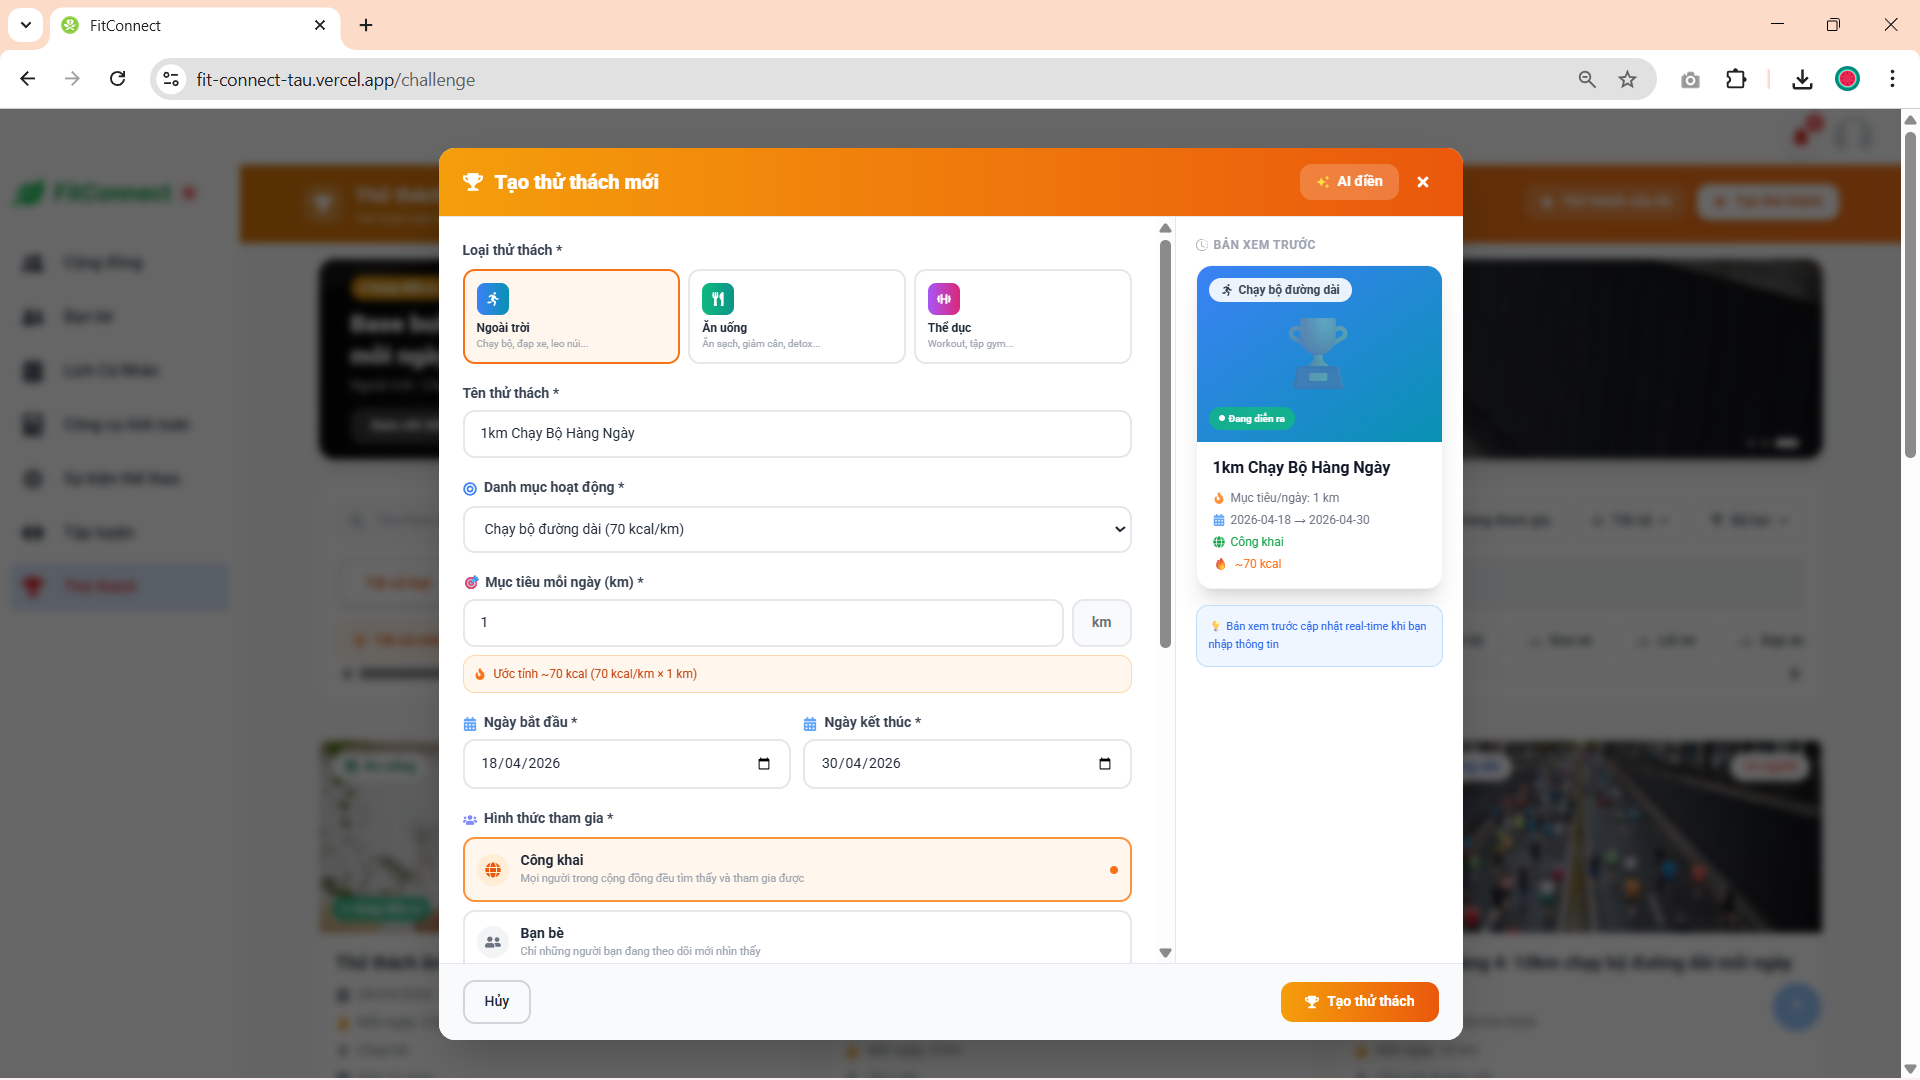
\includegraphics[width=\textwidth]{Images/IMG/nhom4/saukhidungAItaothuthach.png}
        \caption{Hệ thống tự động điền thông tin thử thách sau khi AI xử lý thành công}
        \label{fig:impl_ch_ai_success}
    \end{subfigure}
\end{figure}


    \item Sau khi nhấn Tạo thử thách, hệ thống tự động điều hướng đến trang chi tiết thử thách vừa tạo với đầy đủ thông tin: tên, loại, trạng thái, thời gian, mục tiêu mỗi ngày, số người tham gia và đếm ngược. Người dùng có thể quay lại trang Quản lý Thử thách, nhấn vào ``Thử thách của tôi'' sẽ hiển thị dashboard quản lý với thống kê tổng quan (Tổng đã tạo, Đang diễn ra, Sắp diễn ra, Đã kết thúc) và danh sách thử thách đã tạo cùng thử thách đã tham gia. Bên phải hiển thị thông tin chi tiết của thử thách được chọn với ba tab: Tổng quan, Người tham gia, và Cài đặt.

\begin{figure}[H]
    \centering
    \begin{subfigure}[b]{0.30\textwidth}
        \centering
        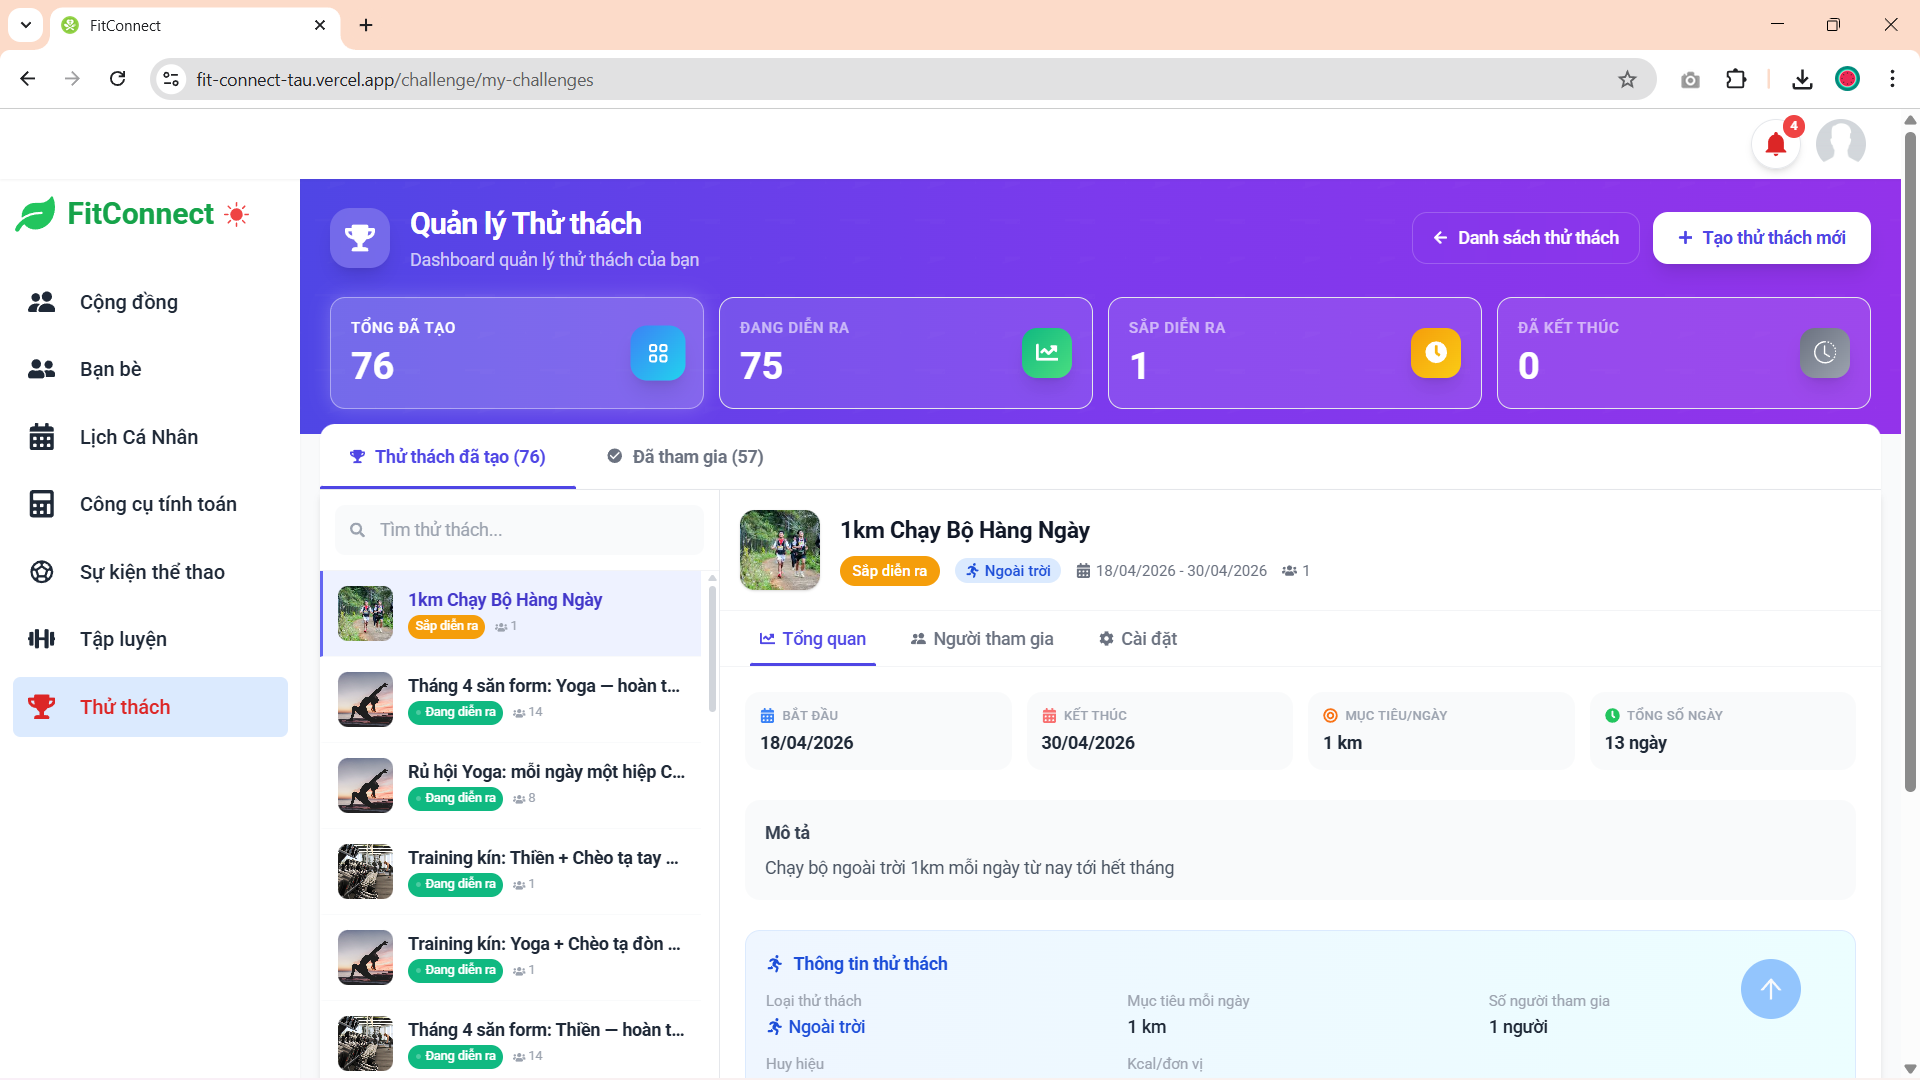
\includegraphics[width=\textwidth]{Images/IMG/nhom4/quanlythuthachvatongquanthu.png}
        \caption{Người dùng xem trang quản lý thử thách và tổng quan thử thách}
        \label{fig:impl_ch_manage}
    \end{subfigure}
    \hfill
    \begin{subfigure}[b]{0.30\textwidth}
        \centering
        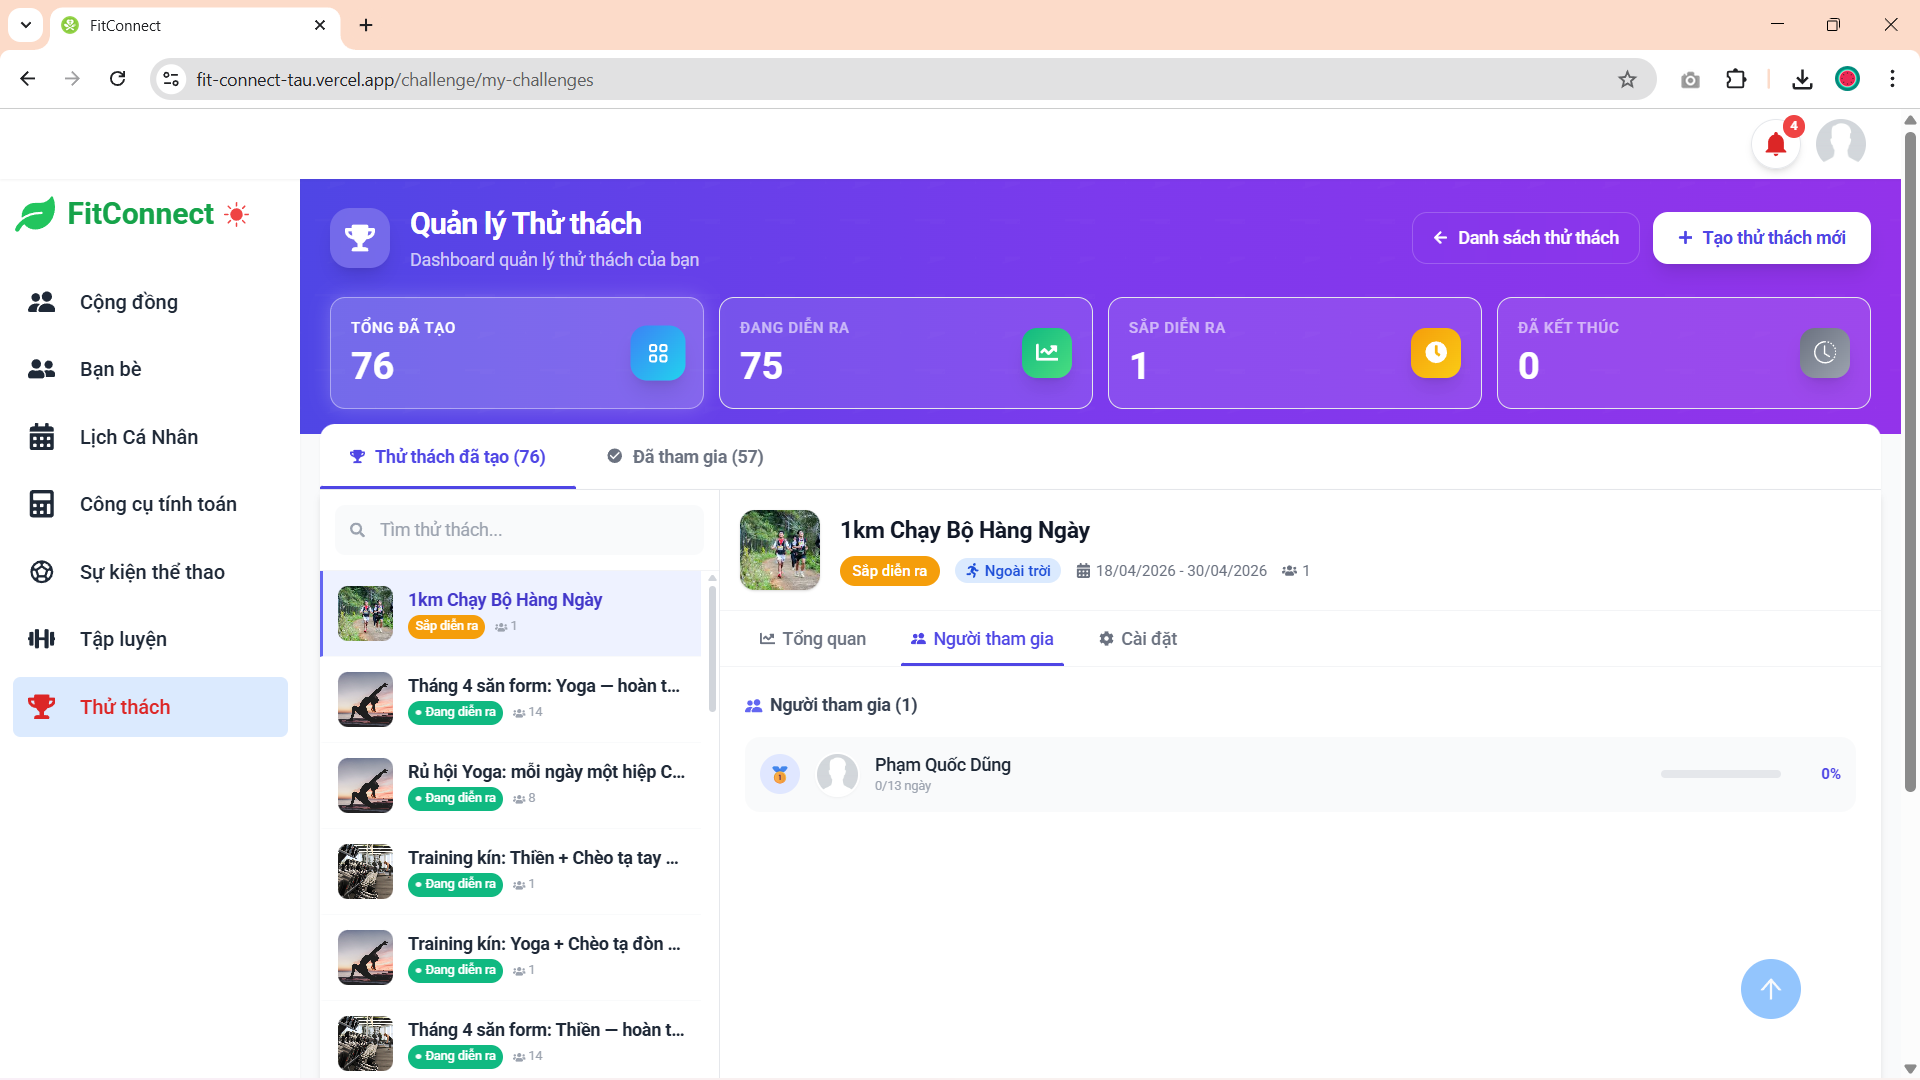
\includegraphics[width=\textwidth]{Images/IMG/nhom4/tabnguoithamgiathuthach.png}
        \caption{Người tạo xem tab Người tham gia thử thách}
        \label{fig:impl_ch_participants}
    \end{subfigure}
    \hfill
    \begin{subfigure}[b]{0.30\textwidth}
        \centering
        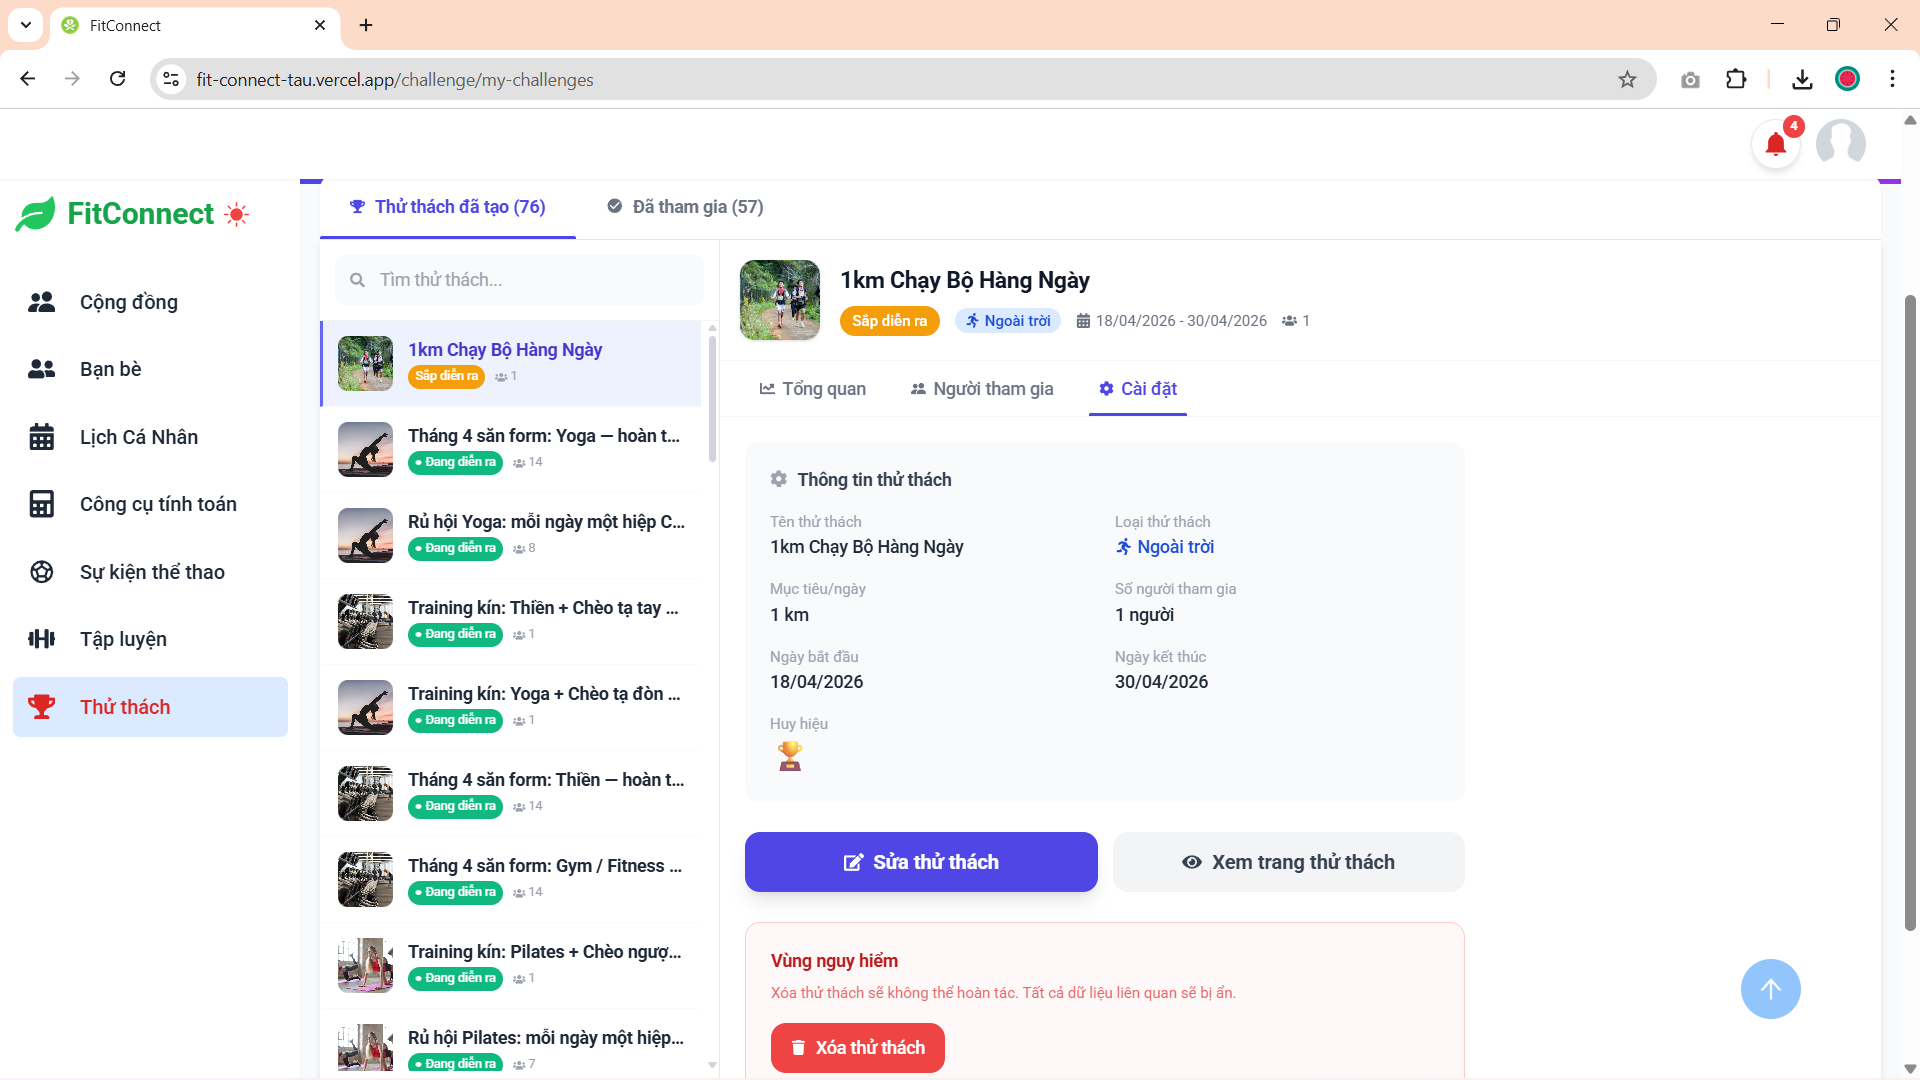
\includegraphics[width=\textwidth]{Images/IMG/nhom4/tabcaidatthuthach.png}
        \caption{Người tạo xem tab Cài đặt thử thách}
        \label{fig:impl_ch_settings}
    \end{subfigure}
\end{figure}


    \item Với chỉnh sửa thử thách: Người tạo có thể nhấn Sửa thử thách ở tab Cài đặt, hệ thống hiển thị modal chỉnh sửa với các thông tin tương tự khi tạo (lưu ý không thể thay đổi loại thử thách sau khi tạo). Sau khi chỉnh sửa, nhấn Lưu thay đổi để cập nhật.

\begin{figure}[H]
    \centering
    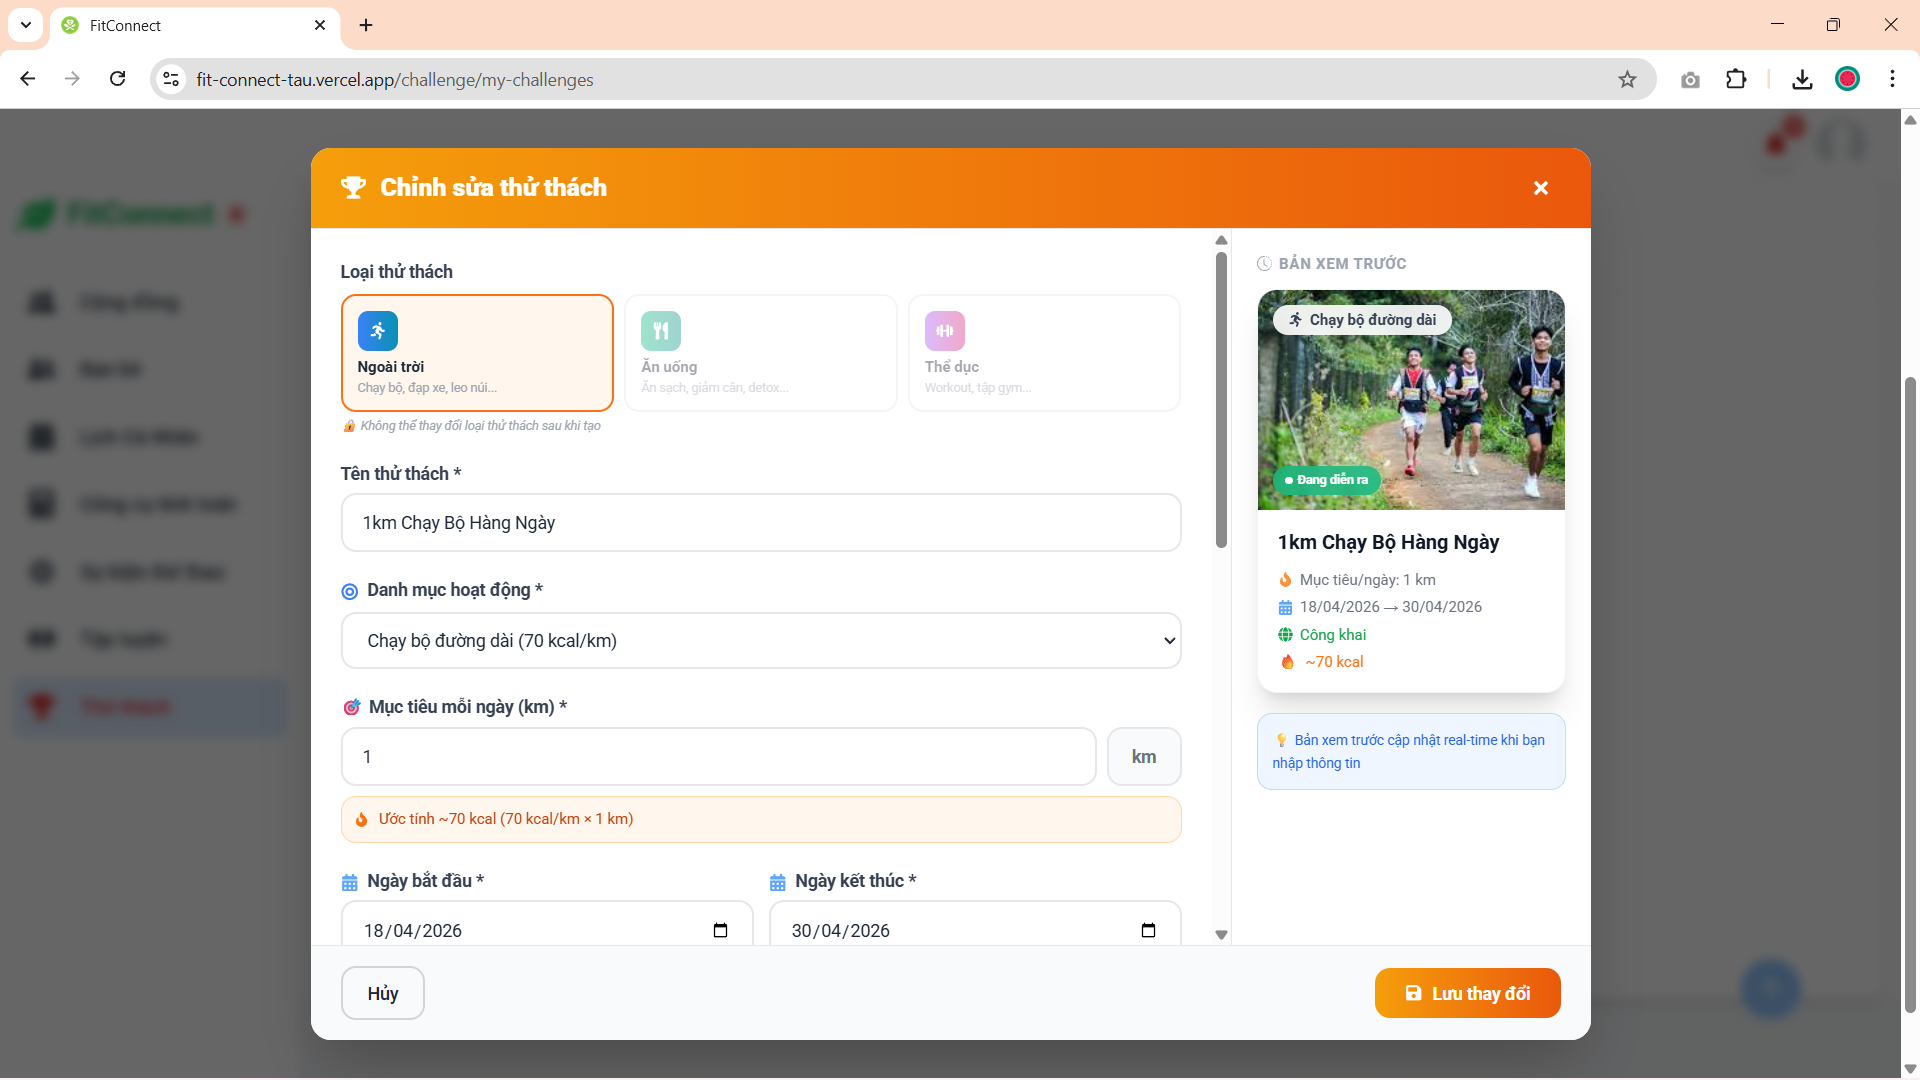
\includegraphics[width=0.60\textwidth]{Images/IMG/nhom4/chinhsuathuthach.png}
    \caption{Người tạo thao tác chỉnh sửa thử thách}
    \label{fig:impl_ch_edit}
\end{figure}

\end{itemize}

\subsubsection{Luồng thao tác tham gia thử thách (Góc độ Người tham gia)}
\begin{itemize}
    \item Với người dùng không phải người tạo, ở trang danh sách thử thách có thể lọc, tìm kiếm và tham gia thử thách. Khi nhấn vào thử thách, hệ thống hiển thị trang chi tiết thử thách với ba tab: Chi tiết, Tiến độ, và Người tham gia.

\begin{figure}[H]
    \centering
    \begin{subfigure}[b]{0.47\textwidth}
        \centering
        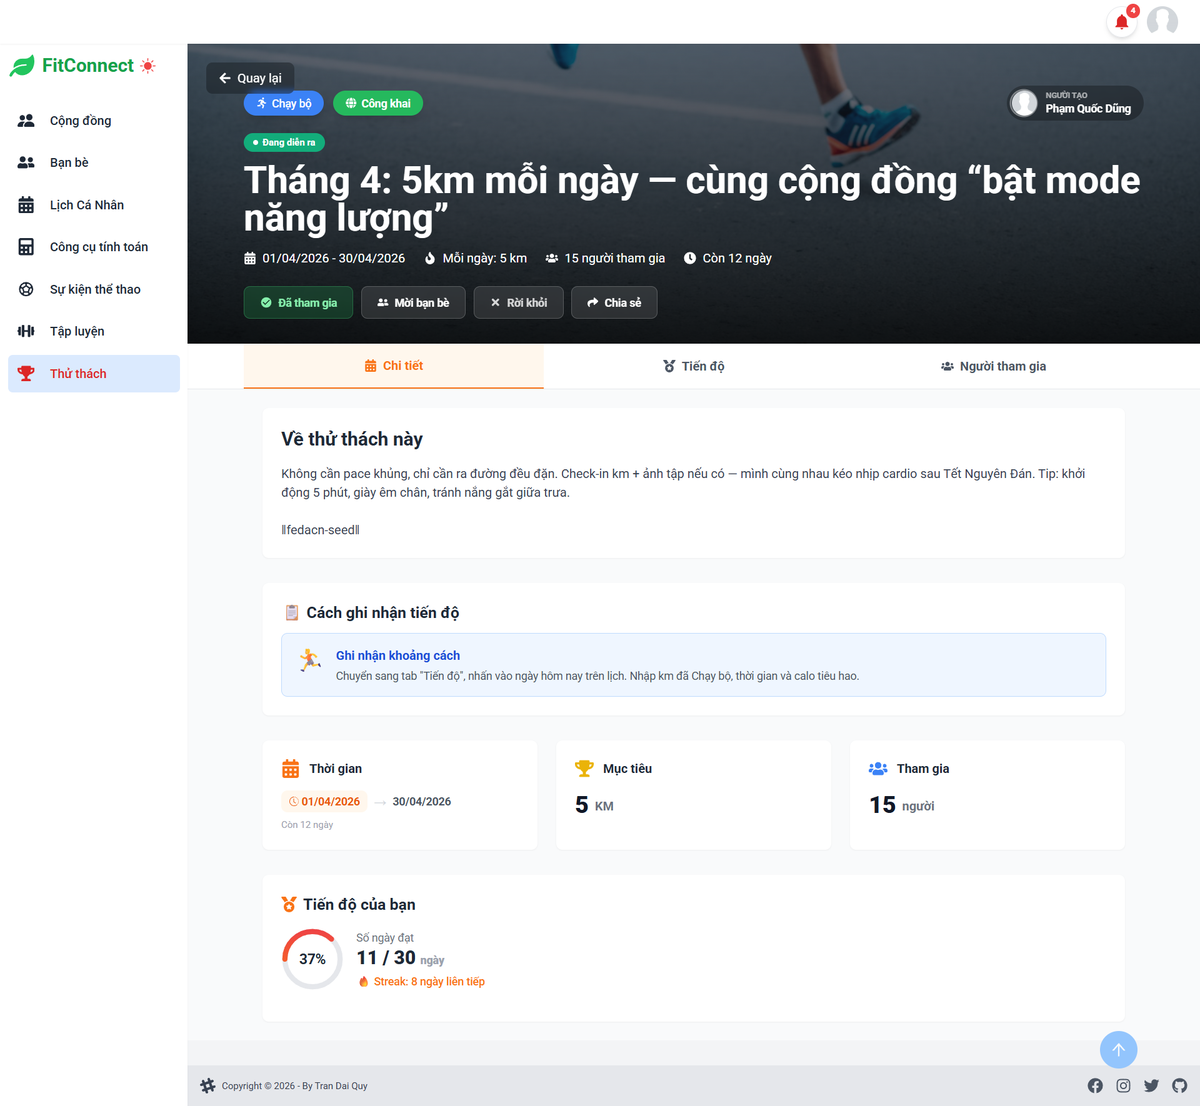
\includegraphics[width=\textwidth]{Images/IMG/nhom4/chitietthuthachdathamgia.png}
        \caption{Người tham gia xem chi tiết thử thách đã tham gia}
        \label{fig:impl_ch_detail}
    \end{subfigure}
    \hfill
    \begin{subfigure}[b]{0.47\textwidth}
        \centering
        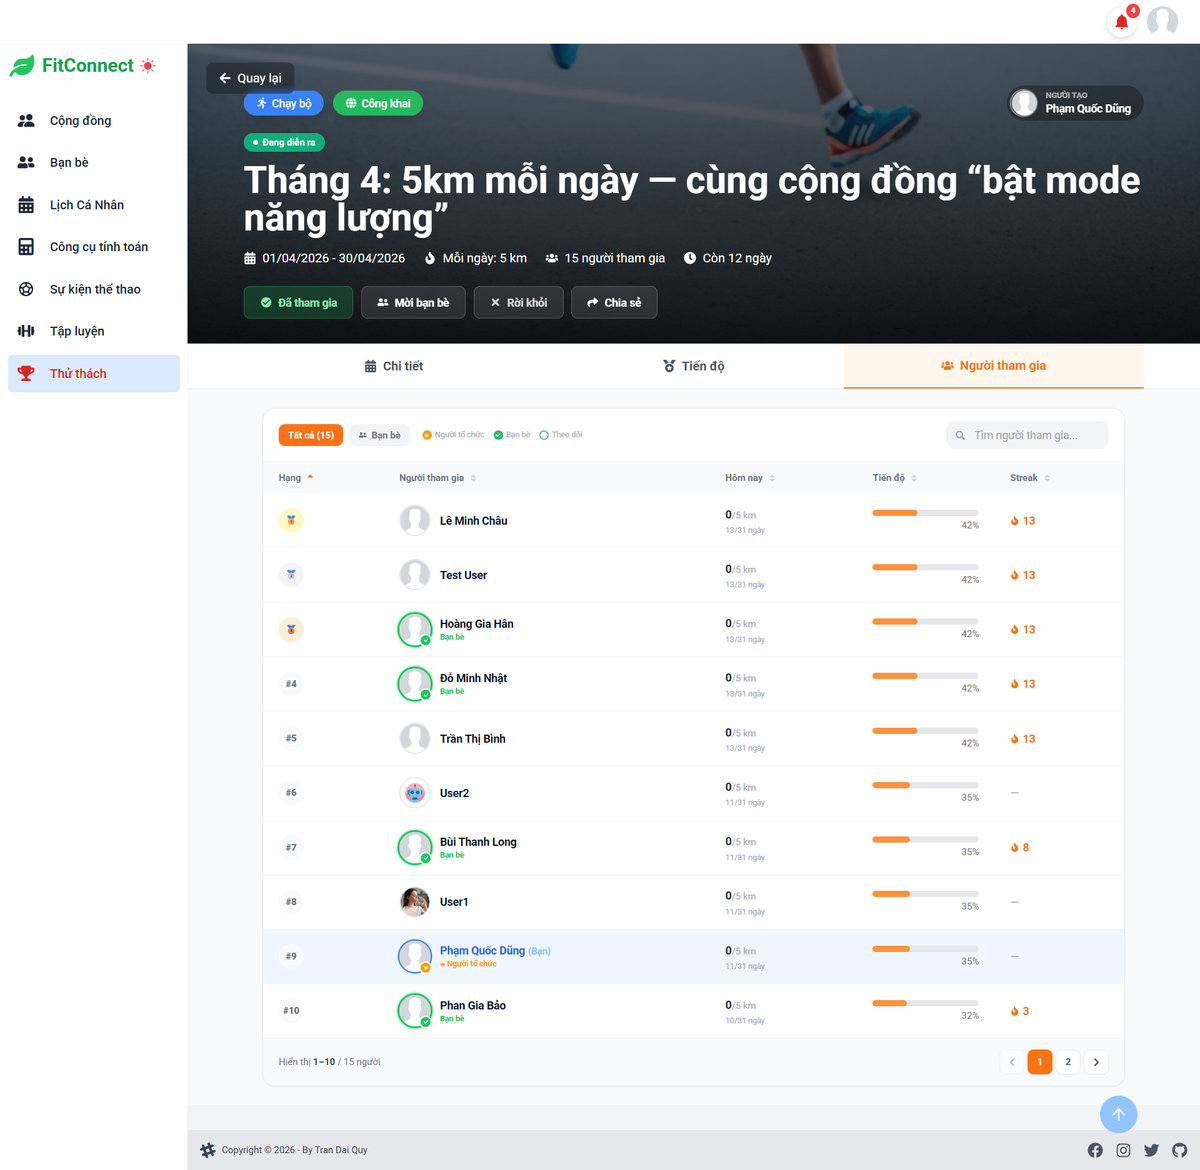
\includegraphics[width=\textwidth]{Images/IMG/nhom4/danhsachnguoithamgiathuthach.png}
        \caption{Người tham gia xem danh sách người tham gia thử thách}
        \label{fig:impl_ch_member_list}
    \end{subfigure}
\end{figure}


    \item Người tham gia có thể xem tab Tiến độ để theo dõi quá trình hoàn thành thử thách. Hệ thống hiển thị: số ngày hoàn thành, tổng số ngày, tỷ lệ hoàn thành, thanh tiến độ tổng thể, và lịch theo tháng hiển thị chi tiết trạng thái từng ngày (Hoàn thành, Đang diễn ra, Đã kết thúc, Chưa diễn ra) kèm quãng đường/số bữa đã ghi nhận.

\begin{figure}[H]
    \centering
    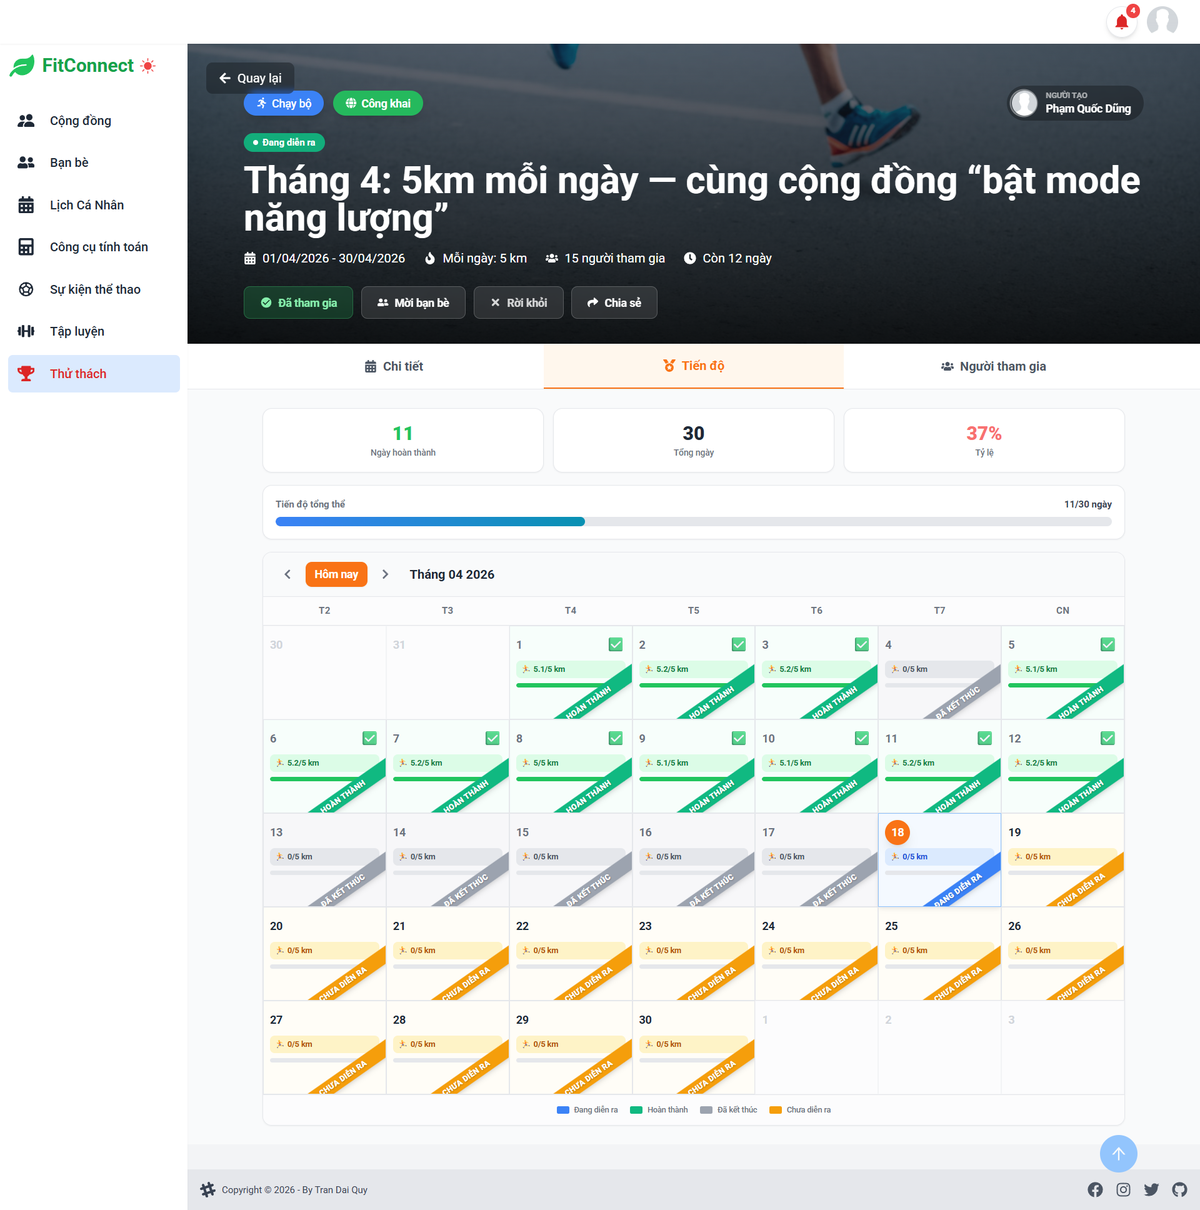
\includegraphics[width=0.60\textwidth]{Images/IMG/nhom4/tabtiendothuthach.png}
    \caption{Người tham gia xem tab Tiến độ thử thách theo lịch}
    \label{fig:impl_ch_progress}
\end{figure}


    \item Tại tab Tiến độ hoặc khi xem chi tiết hoạt động của người tham gia khác, người dùng có thể tương tác bằng cách gửi bình luận. Hệ thống hiển thị phần bình luận bên dưới chi tiết hoạt động (ví dụ: ngày ghi nhận, số km/bữa ăn), cho phép người tham gia nhập thông điệp động viên và trao đổi với các thành viên khác.

\begin{figure}[H]
    \centering
    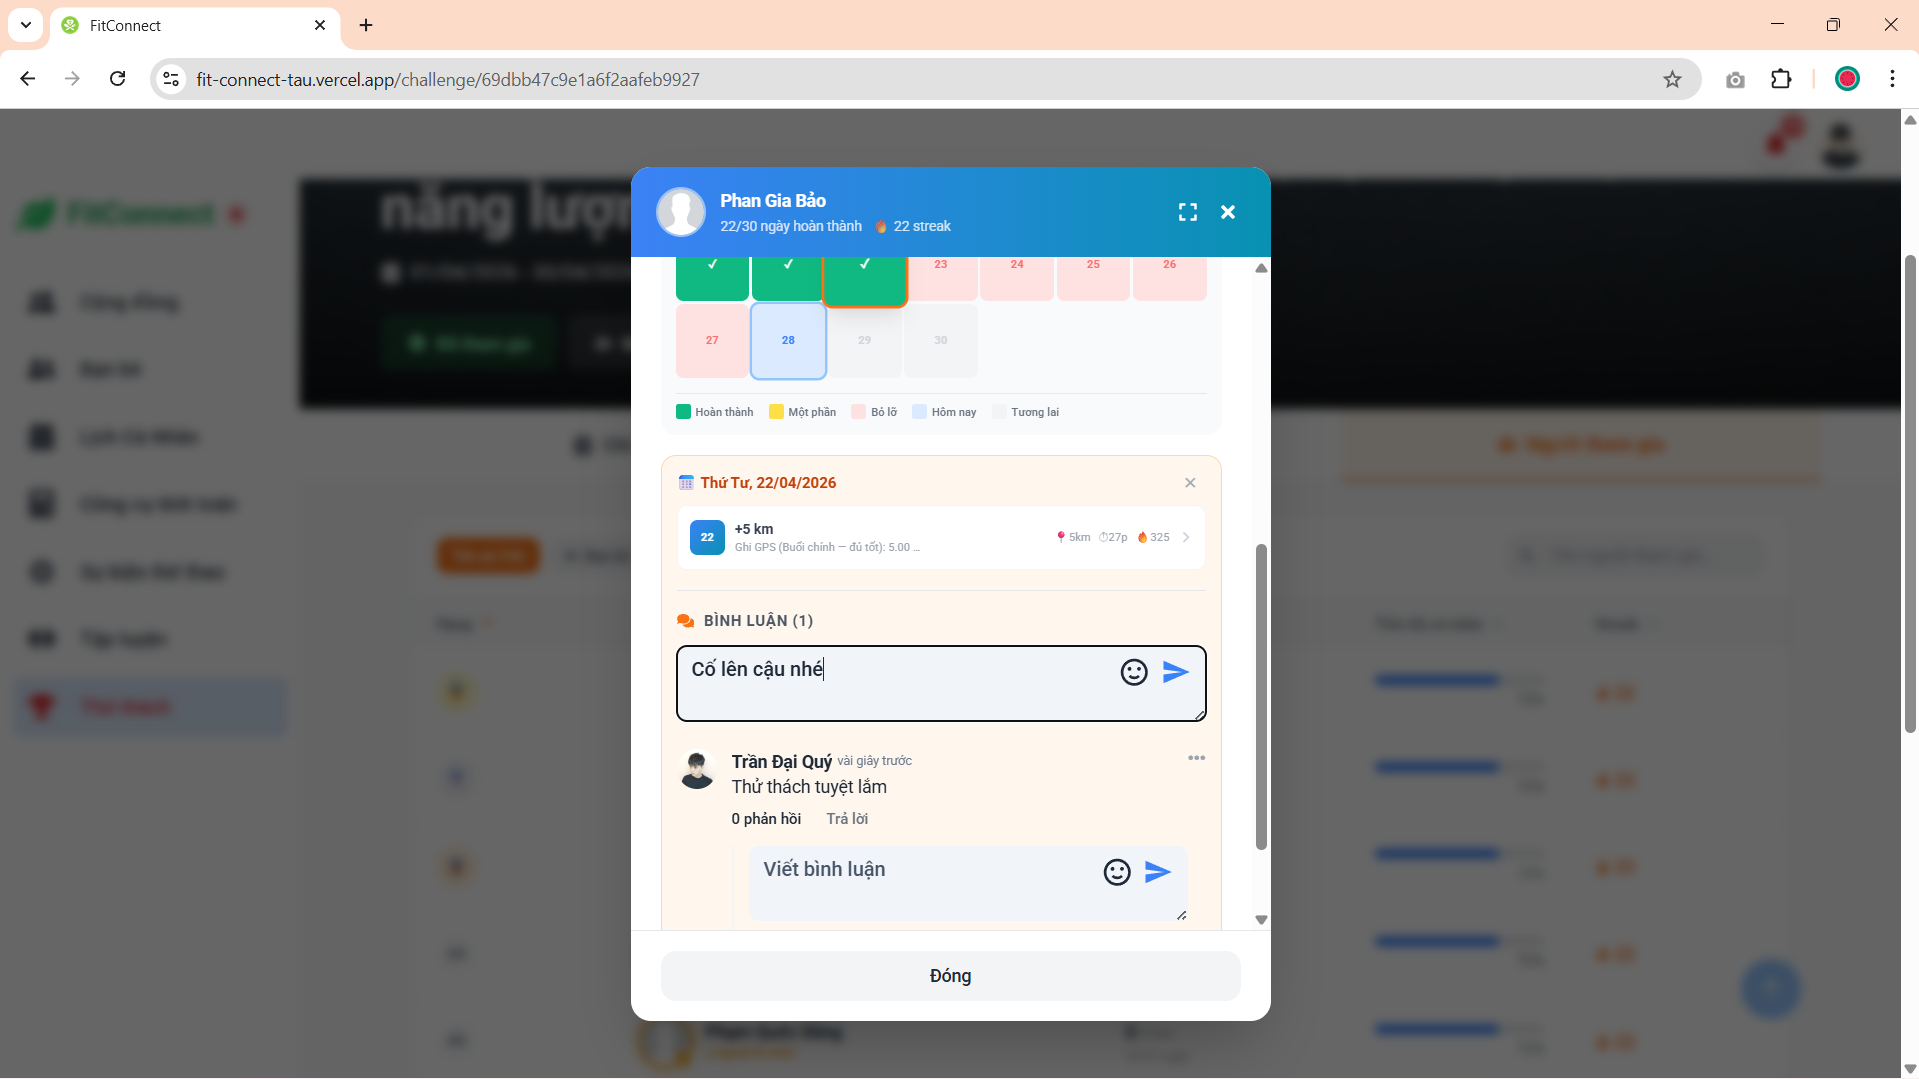
\includegraphics[width=0.60\textwidth]{Images/IMG/nhom4/binhluanthuthachnguoithamgia.png}
    \caption{Người tham gia bình luận vào hoạt động thử thách của thành viên khác}
    \label{fig:impl_ch_comment}
\end{figure}


    \item Người tham gia có thể chia sẻ thử thách lên trang Cộng đồng; bài viết thử thách sẽ tự động xuất hiện trên Bảng tin cộng đồng.

\begin{figure}[H]
    \centering
    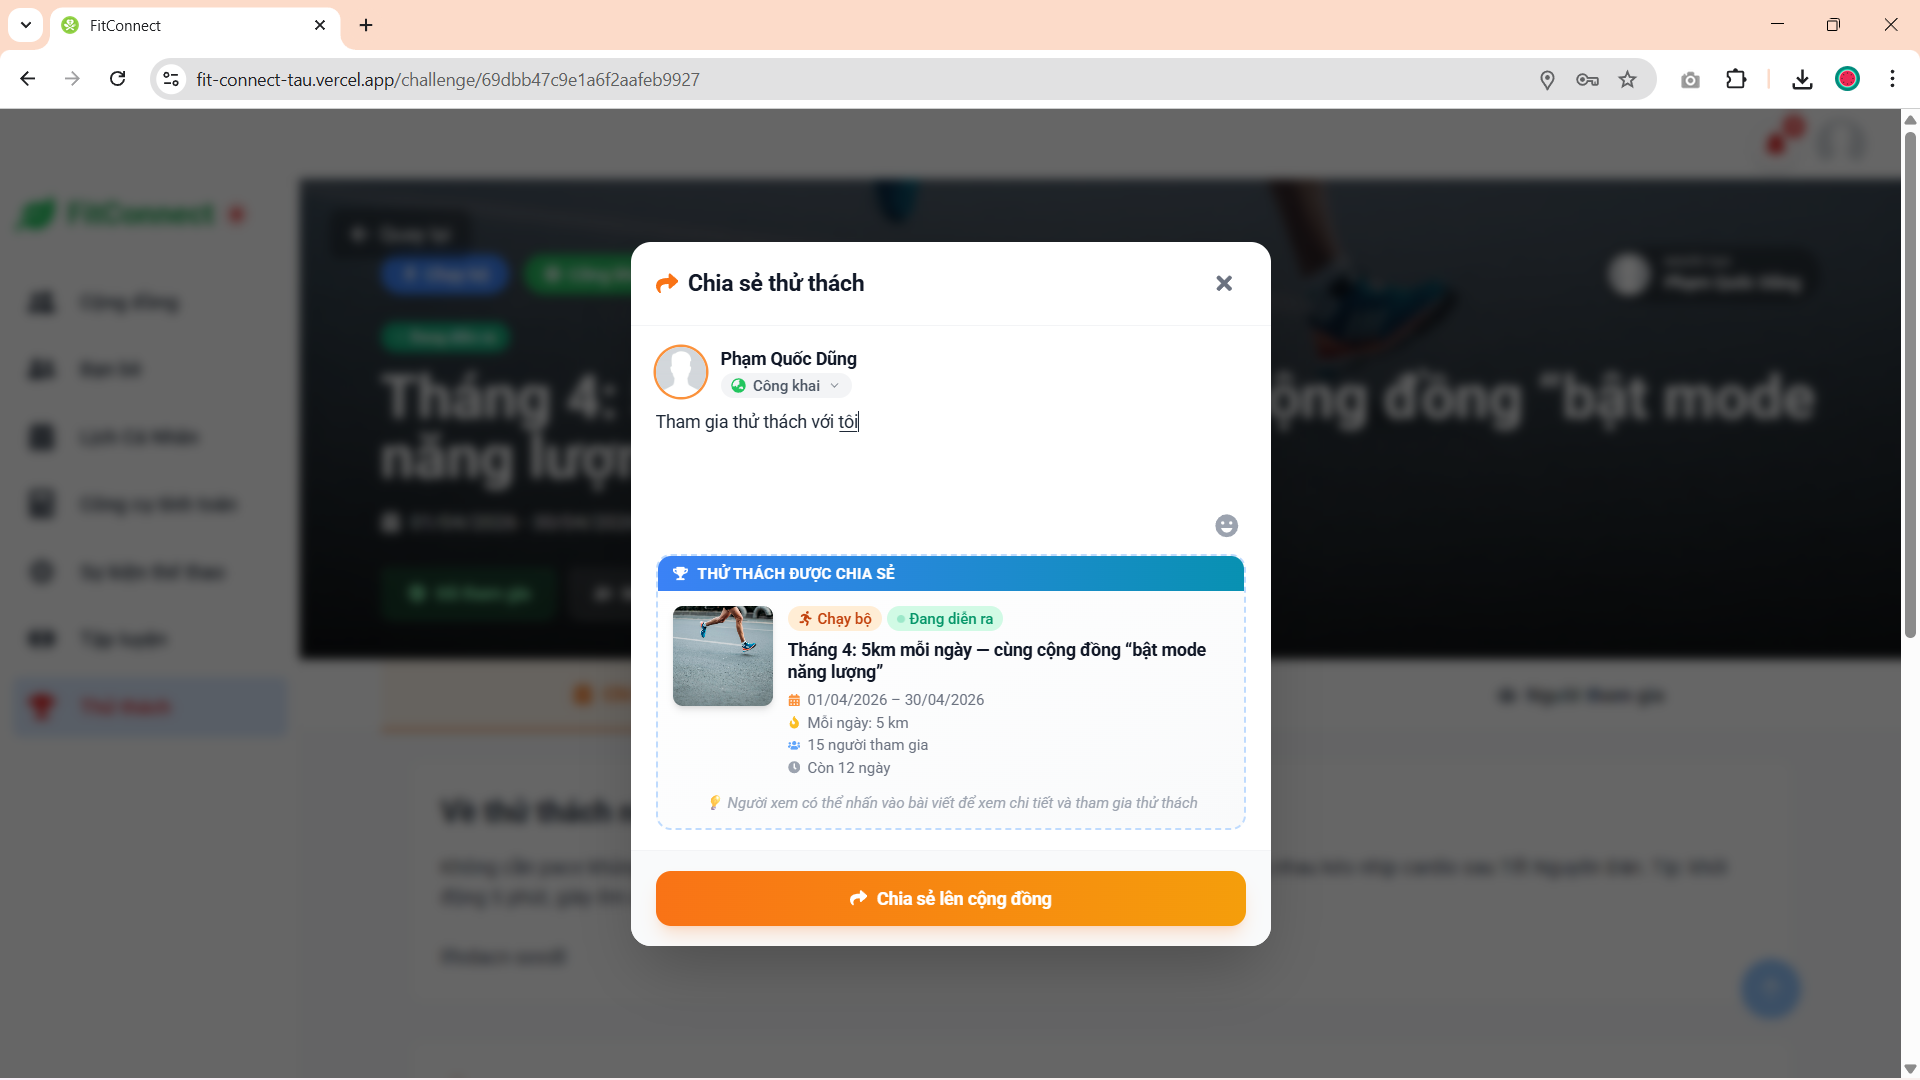
\includegraphics[width=0.60\textwidth]{Images/IMG/nhom4/chiasethuthach.png}
    \caption{Người tham gia thao tác chia sẻ thử thách lên cộng đồng}
    \label{fig:impl_ch_share}
\end{figure}


    \item Người tham gia có thể mời bạn bè tham gia thử thách. Hệ thống hiển thị modal tìm kiếm và mời bạn bè, bạn bè được mời sẽ nhận được thông báo.

\begin{figure}[H]
    \centering
    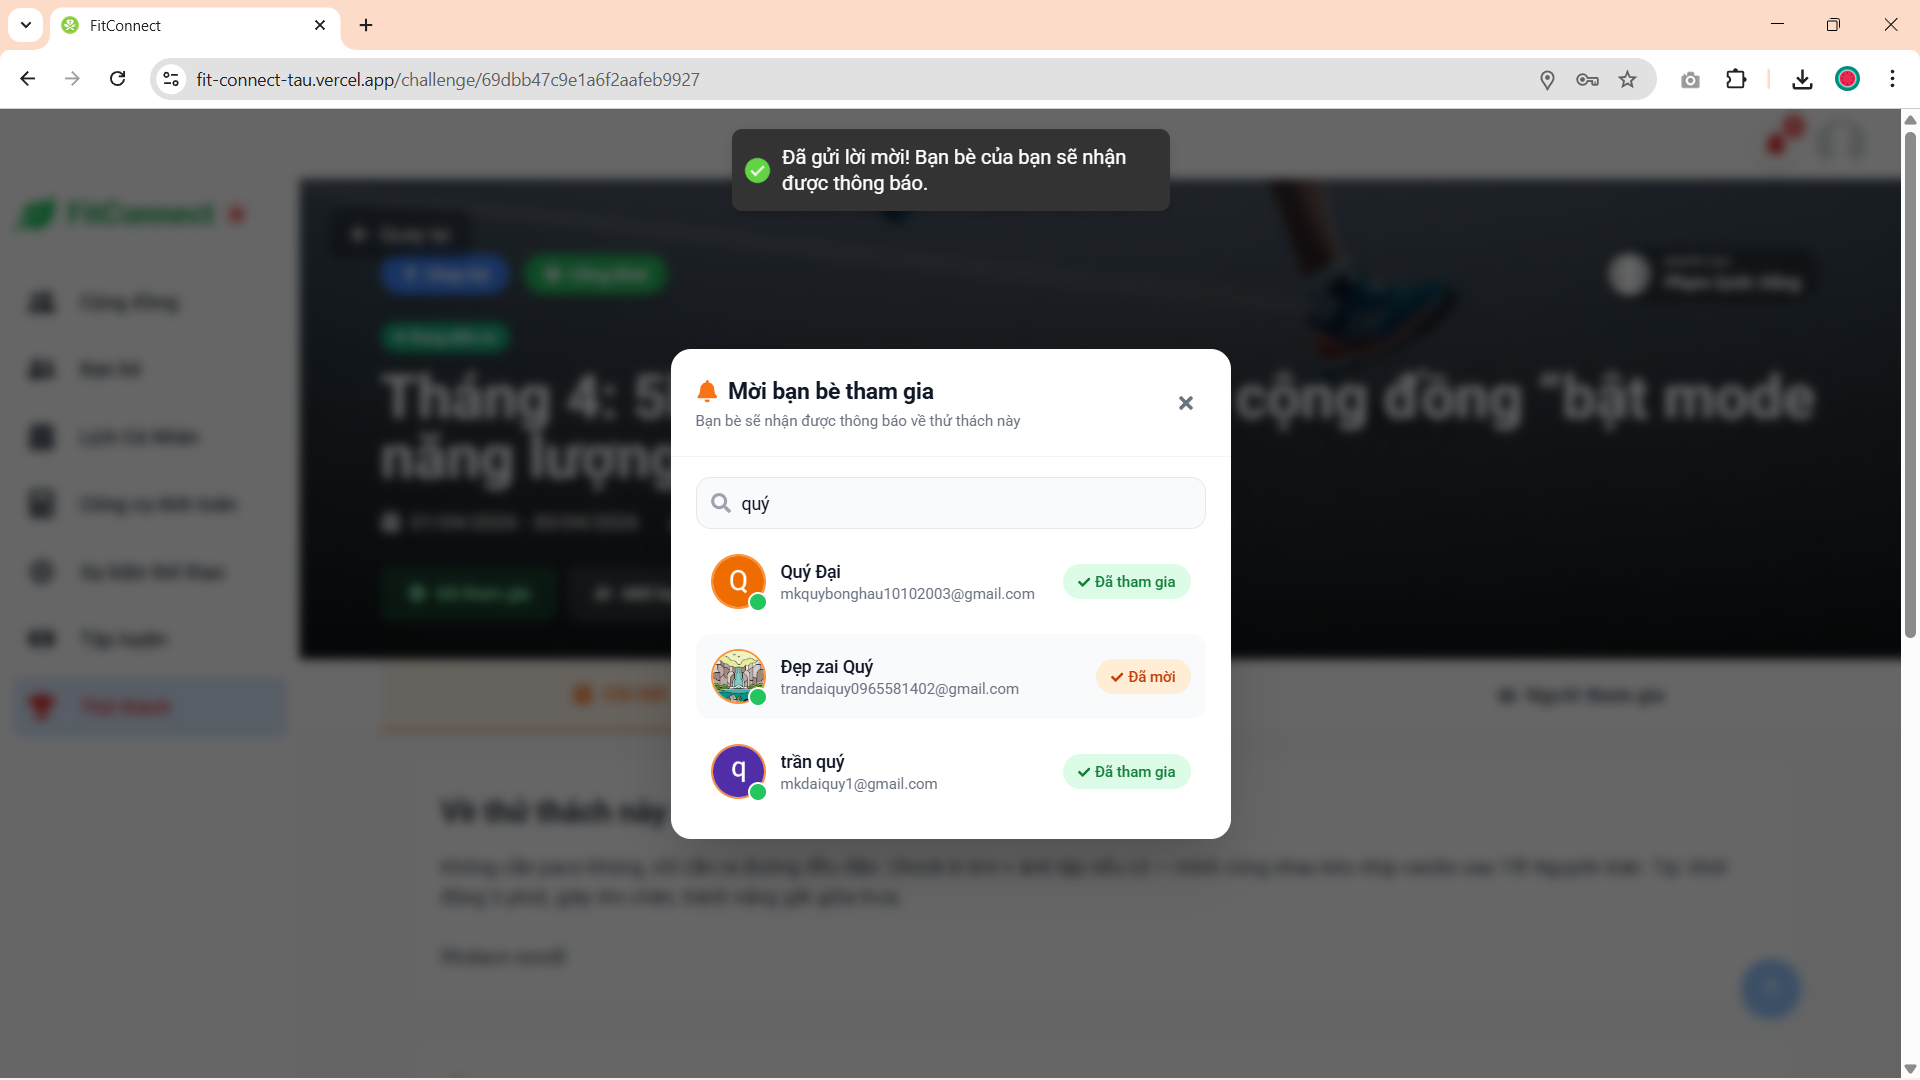
\includegraphics[width=0.60\textwidth]{Images/IMG/nhom4/moibanbethamgiathuthach.png}
    \caption{Người tham gia thao tác mời bạn bè tham gia thử thách}
    \label{fig:impl_ch_invite}
\end{figure}


    \item Người tham gia có thể báo cáo thử thách vi phạm lên Quản trị viên bằng cách nhập lý do báo cáo và nhấn Gửi báo cáo.

\begin{figure}[H]
    \centering
    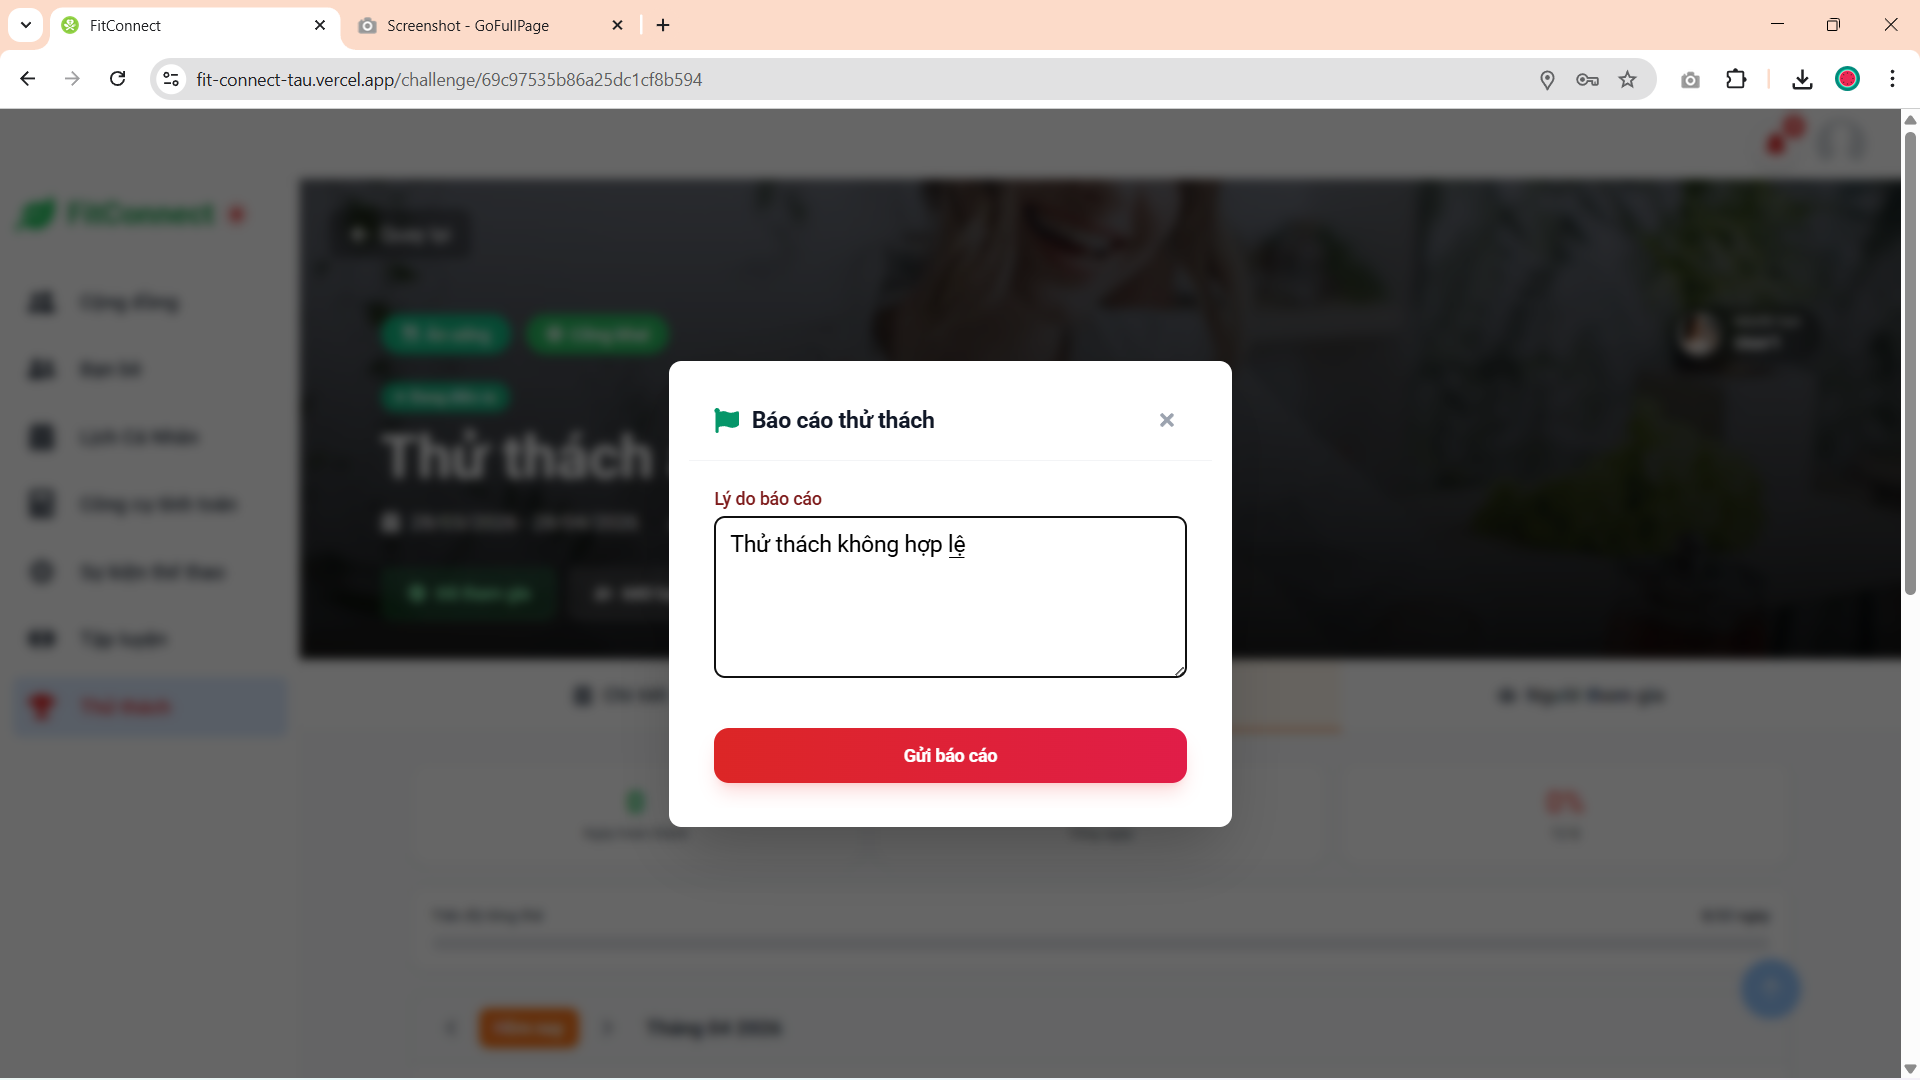
\includegraphics[width=0.60\textwidth]{Images/IMG/nhom4/baocaothuthach.png}
    \caption{Người tham gia thao tác báo cáo thử thách}
    \label{fig:impl_ch_report}
\end{figure}

\end{itemize}

\textbf{Ghi nhận tiến độ thử thách hàng ngày:}

\textbf{a) Đối với thử thách Ngoài trời (chạy bộ, đạp xe,...):}
\begin{itemize}
    \item Người tham gia nhấn vào ngày hiện tại trên lịch tiến độ, hệ thống hiển thị modal bắt đầu ghi với thông tin mục tiêu ngày (km) và nút Bắt đầu ghi. Khi nhấn Bắt đầu ghi, hệ thống chuyển sang trang GPS Tracking hiển thị bản đồ với vị trí hiện tại, quãng đường (km), thời gian, tốc độ (km/h), calories (kcal) và thanh tiến độ mục tiêu ngày.

\begin{figure}[H]
    \centering
    \begin{subfigure}[b]{0.47\textwidth}
        \centering
        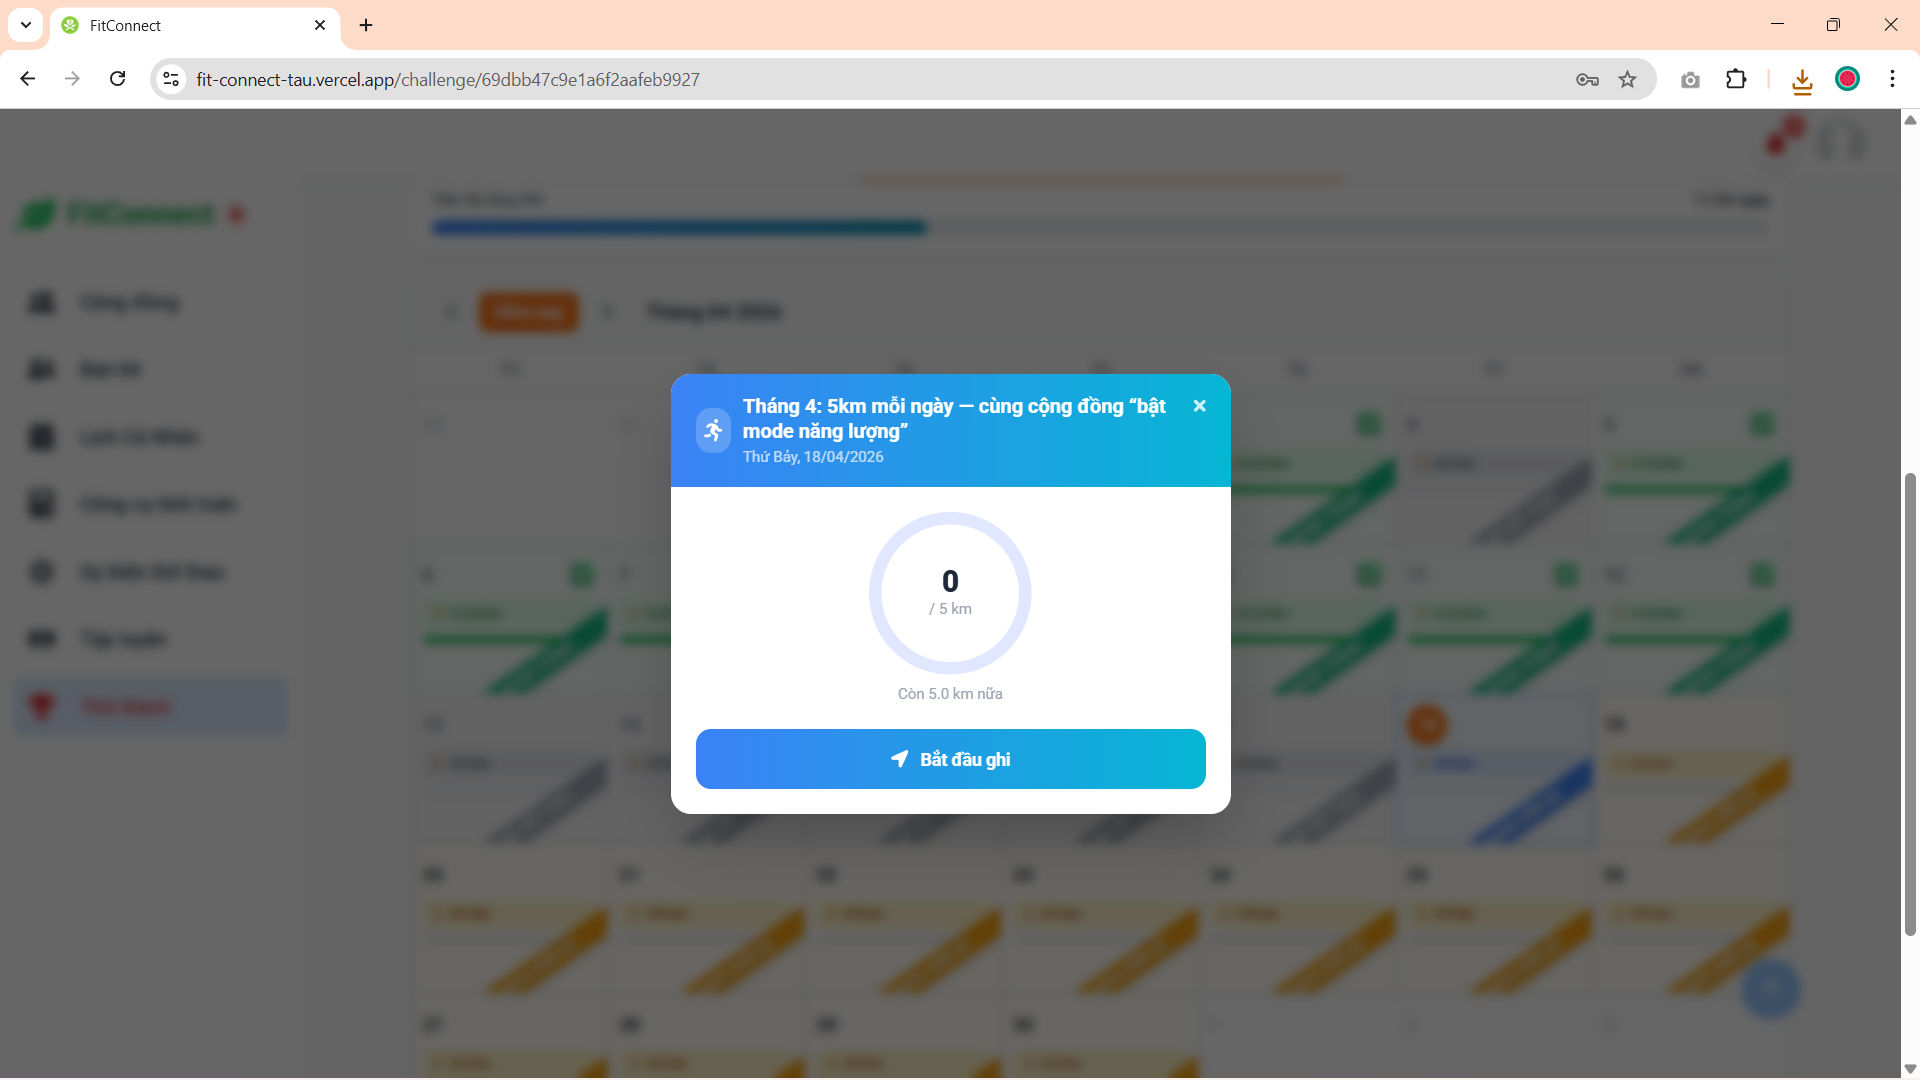
\includegraphics[width=\textwidth]{Images/IMG/nhom4/manhinhbatdauthuchienttchaybo.png}
        \caption{Hệ thống hiển thị modal bắt đầu thực hiện thử thách chạy bộ}
        \label{fig:impl_ch_start_run}
    \end{subfigure}
    \hfill
    \begin{subfigure}[b]{0.47\textwidth}
        \centering
        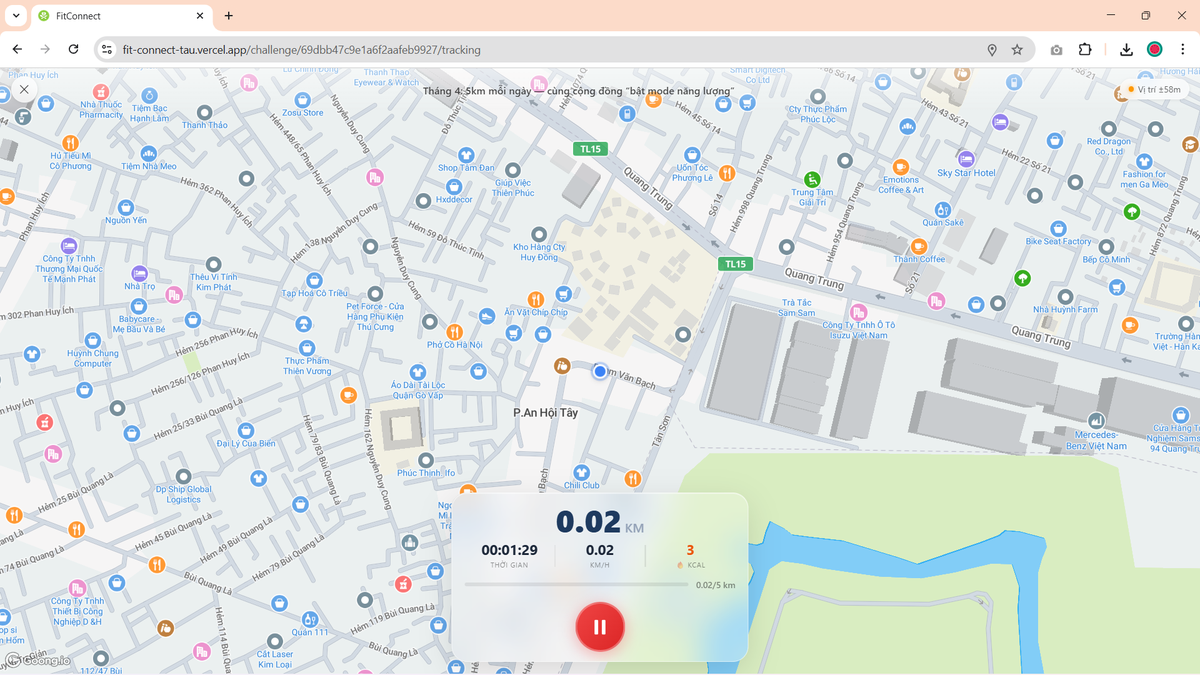
\includegraphics[width=\textwidth]{Images/IMG/nhom4/giaodienthuthachchaybo.png}
        \caption{Người tham gia ghi tiến độ thử thách chạy bộ bằng GPS tracking}
        \label{fig:impl_ch_gps}
    \end{subfigure}
\end{figure}


    \item Khi nhấn hoàn thành, hệ thống tổng hợp và hiển thị kết quả: quãng đường (km), thời gian, calories (kcal), vận tốc trung bình. Người tham gia nhấn Xác nhận để lưu kết quả vào tiến độ thử thách.

\end{itemize}

\textbf{b) Đối với thử thách Ăn uống (ăn sạch, giảm cân, detox,...):}
\begin{itemize}
    \item Người tham gia nhấn vào ngày hiện tại trên lịch tiến độ, hệ thống hiển thị modal bắt đầu ghi tiến độ bữa ăn với thông tin mục tiêu ngày (số bữa), danh sách các lần hoạt động đã ghi nhận và nút Bắt đầu thực hiện.

\begin{figure}[H]
    \centering
    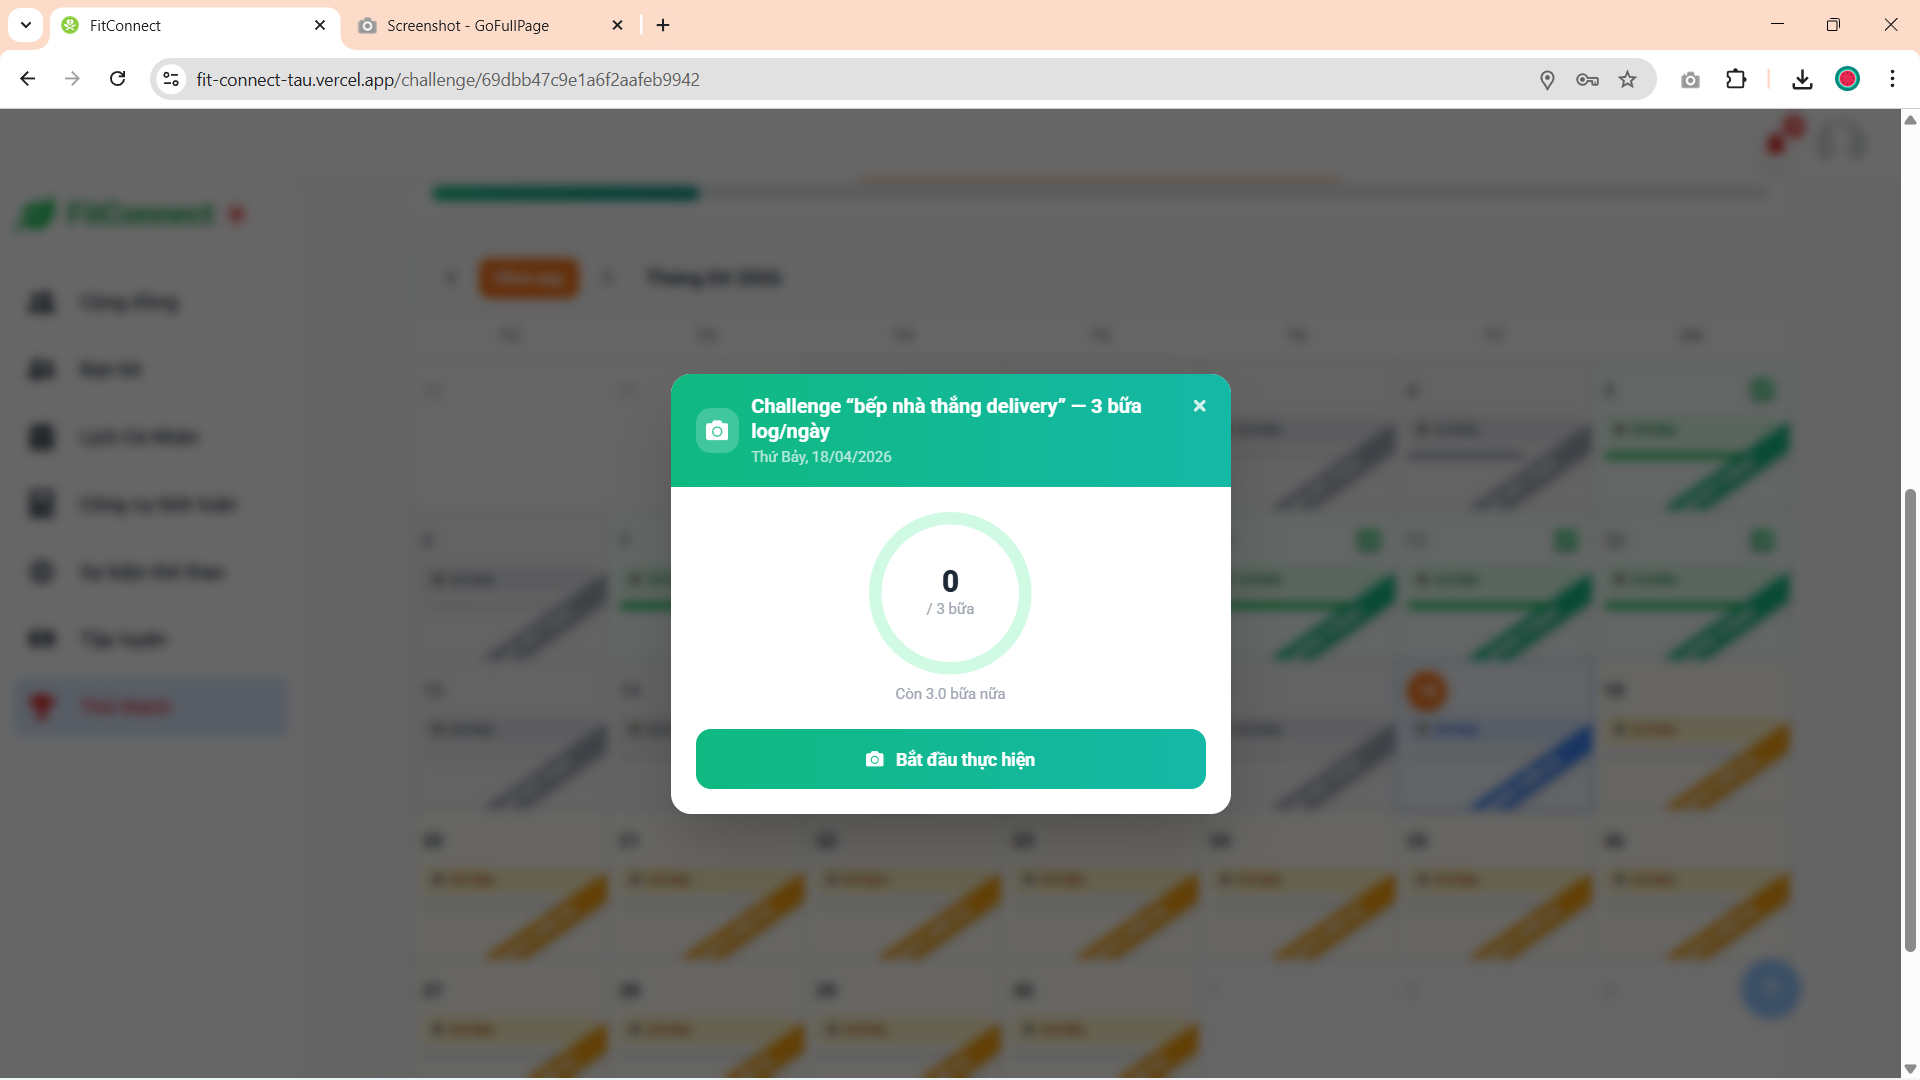
\includegraphics[width=0.60\textwidth]{Images/IMG/nhom4/1modalbatdaughitiendobuaan.png}
    \caption{Hệ thống hiển thị modal bắt đầu ghi tiến độ bữa ăn}
    \label{fig:impl_ch_food_start}
\end{figure}


    \item Khi nhấn Bắt đầu thực hiện, hệ thống hiển thị modal Ghi nhận bữa ăn với các thông tin: loại bữa ăn (Bữa sáng, Bữa trưa, Bữa tối, Bữa phụ), tên món ăn, ảnh bữa ăn (bắt buộc để Check-in, AI sẽ tự động xác minh ảnh), kcal ước tính (tùy chọn), và mô tả.

\begin{figure}[H]
    \centering
    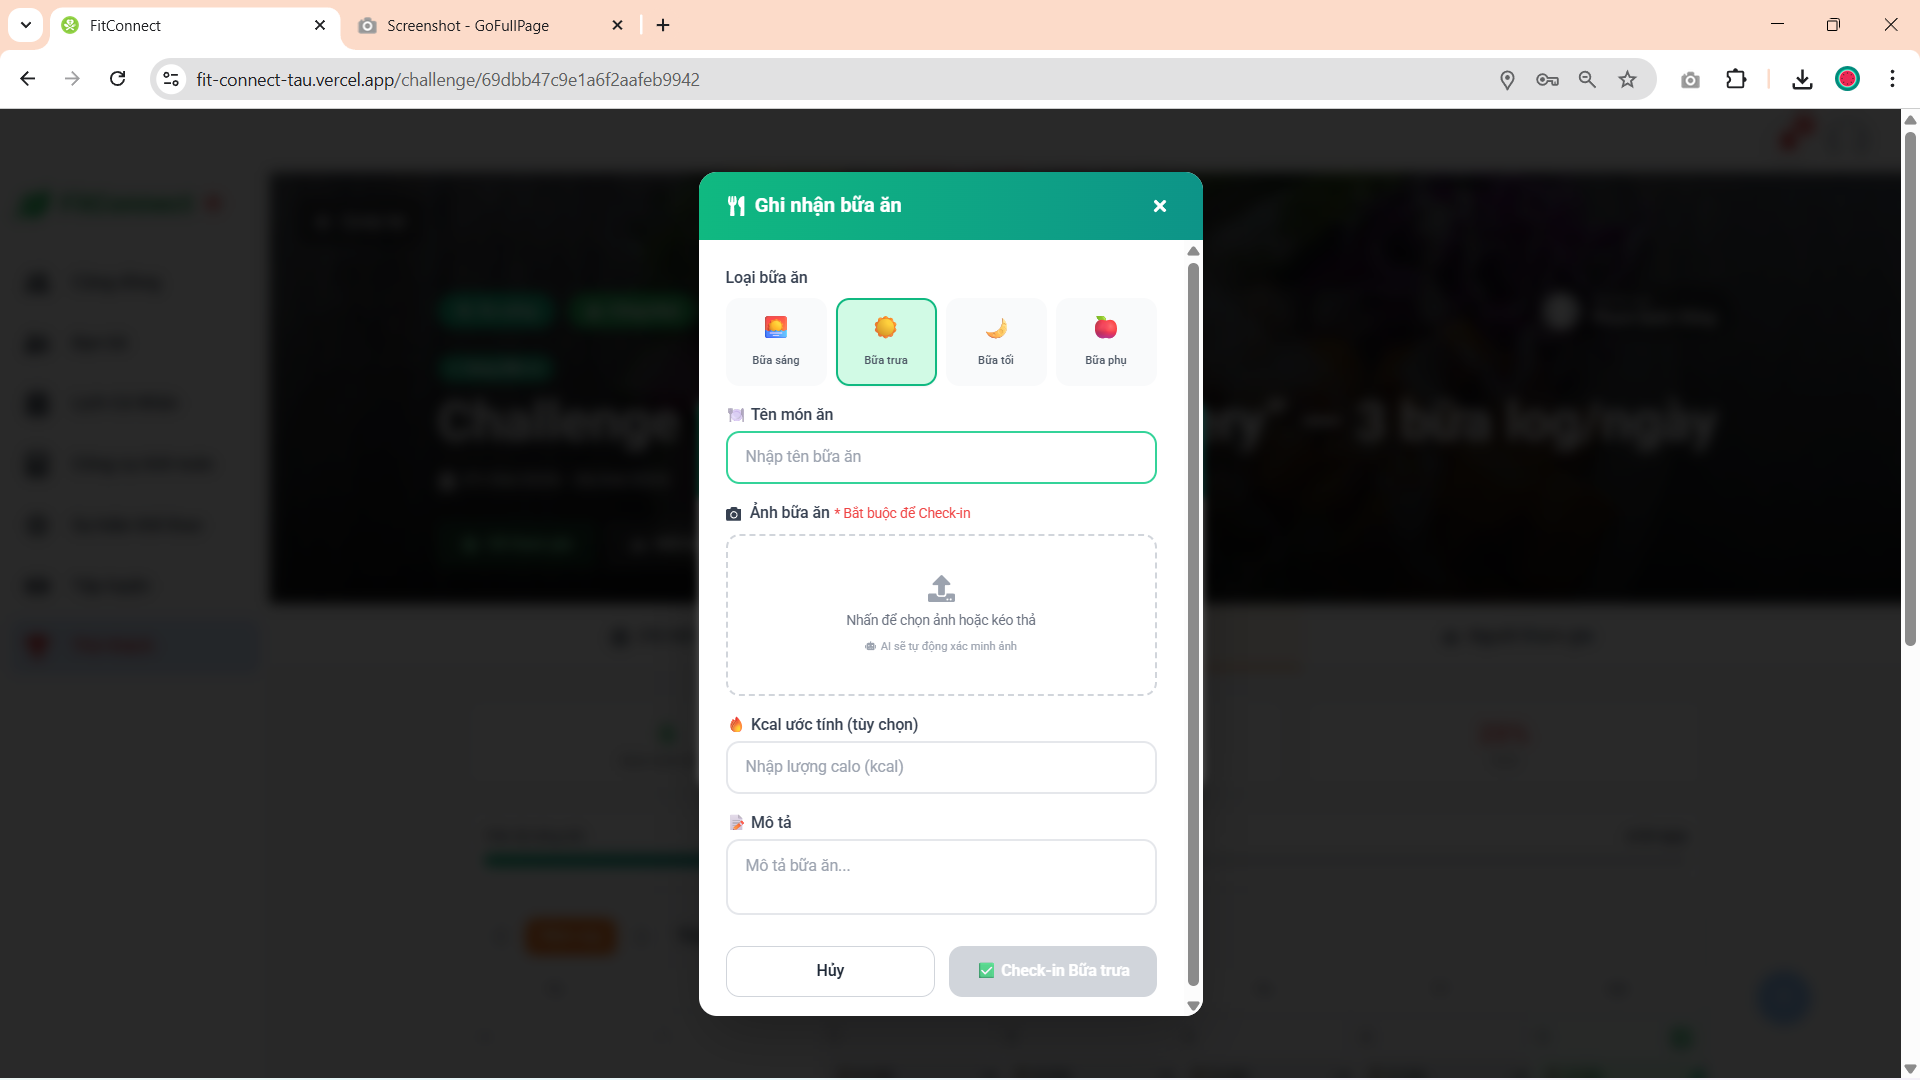
\includegraphics[width=0.60\textwidth]{Images/IMG/nhom4/1modalcheckingbuaan.png}
    \caption{Hệ thống hiển thị modal ghi nhận bữa ăn}
    \label{fig:impl_ch_food_form}
\end{figure}


    \item Sau khi tải ảnh bữa ăn lên, hệ thống sử dụng AI tự động xác minh ảnh. Nếu ảnh hợp lệ, hệ thống hiển thị thông báo ``Ảnh hợp lệ'' kèm nhận xét của AI về ảnh, và cho phép Check-in bữa ăn.

\begin{figure}[H]
    \centering
    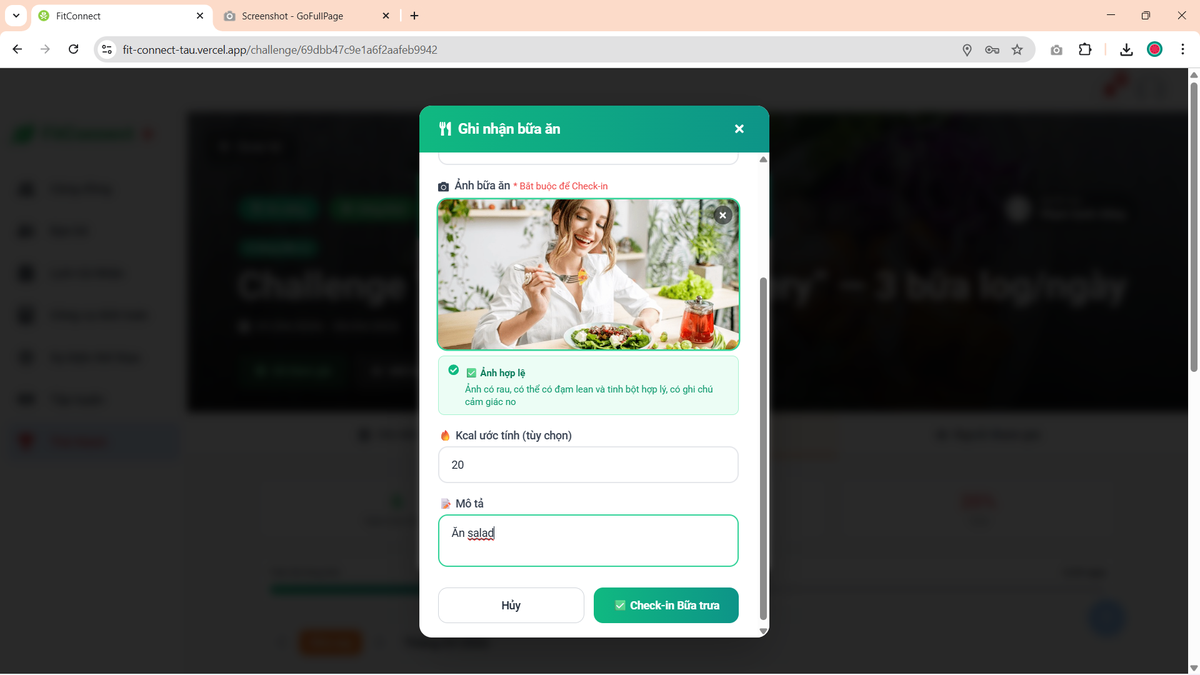
\includegraphics[width=0.60\textwidth]{Images/IMG/nhom4/1checkingbuaanhople.png}
    \caption{Hệ thống AI xác minh ảnh bữa ăn hợp lệ}
    \label{fig:impl_ch_food_valid}
\end{figure}


    \item Nếu ảnh không phù hợp (không phải ảnh bữa ăn), hệ thống hiển thị thông báo ``Ảnh không phù hợp'' kèm giải thích, và cảnh báo ``Nếu tiếp tục, hệ thống vẫn ghi nhận nhưng hoạt động này sẽ KHÔNG được tính vào tiến độ chung''. Người dùng có thể chọn ảnh khác hoặc vẫn tiếp tục.

\begin{figure}[H]
    \centering
    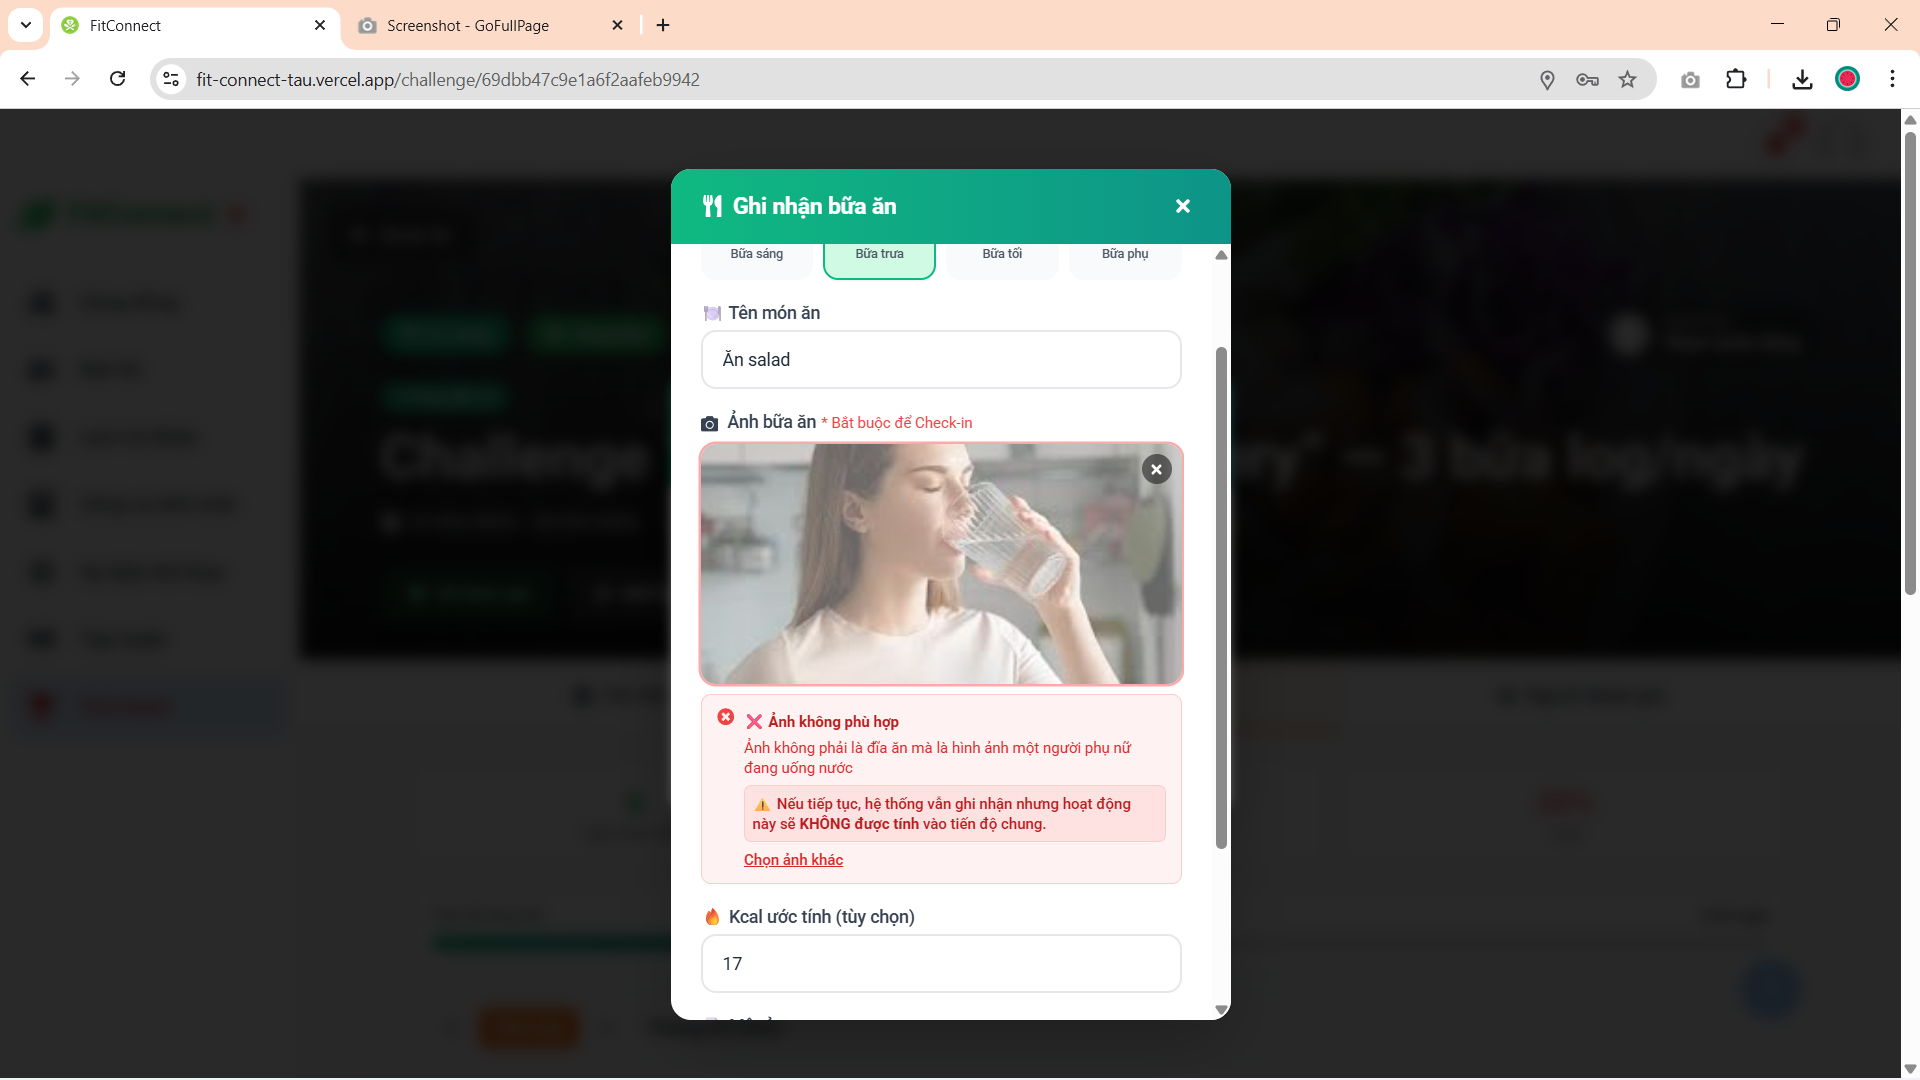
\includegraphics[width=0.60\textwidth]{Images/IMG/nhom4/1checkbuaankhonghople.png}
    \caption{Hệ thống AI xác minh ảnh bữa ăn không hợp lệ}
    \label{fig:impl_ch_food_invalid}
\end{figure}


    \item Sau khi Check-in bữa ăn hợp lệ, hệ thống hiển thị modal thông tin bữa ăn đã ghi nhận với badge ``AI Verified'', thông tin đóng góp (+1 bữa), năng lượng (kcal), nhận xét AI, và tiến độ hôm nay.

\begin{figure}[H]
    \centering
    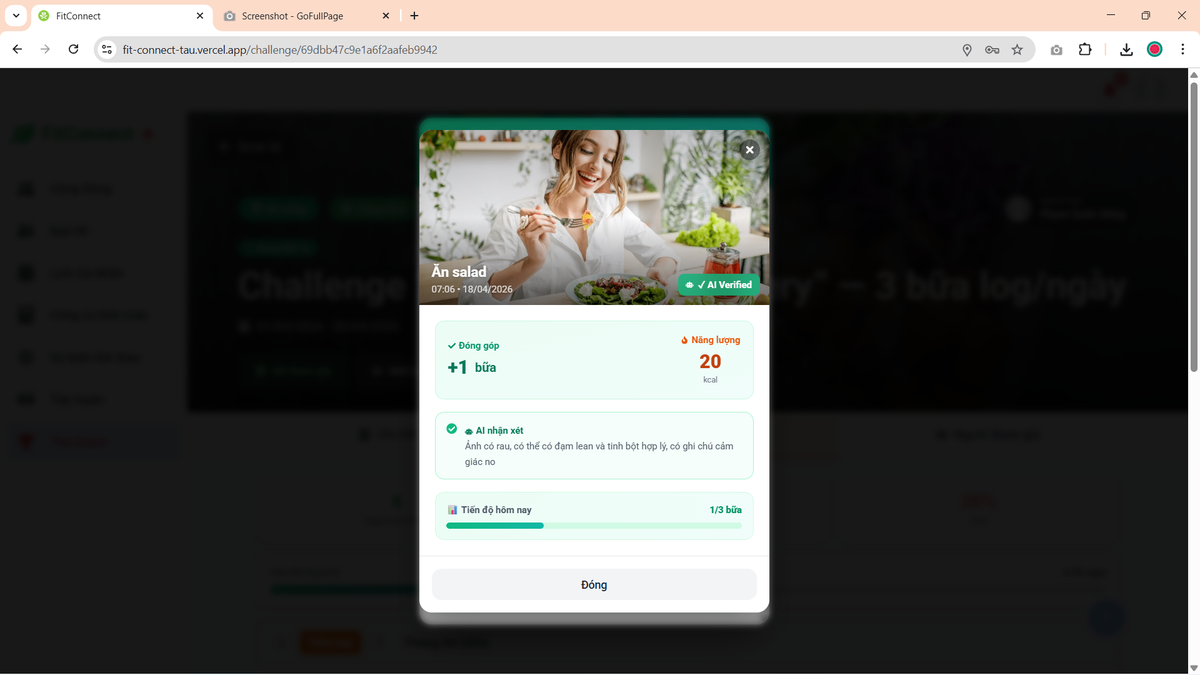
\includegraphics[width=0.60\textwidth]{Images/IMG/nhom4/1xemthongtinbuaandachecking.png}
    \caption{Hệ thống hiển thị thông tin bữa ăn đã được AI xác minh}
    \label{fig:impl_ch_food_verified}
\end{figure}


    \item Hệ thống cập nhật modal tiến độ ngày với bữa ăn hợp lệ được tính vào tiến độ (hiển thị xanh), bữa ăn không hợp lệ vẫn được ghi nhận nhưng hiển thị ghi chú ``Không hợp lệ'' và không tính vào tiến độ chung.

\begin{figure}[H]
    \centering
    \begin{subfigure}[b]{0.47\textwidth}
        \centering
        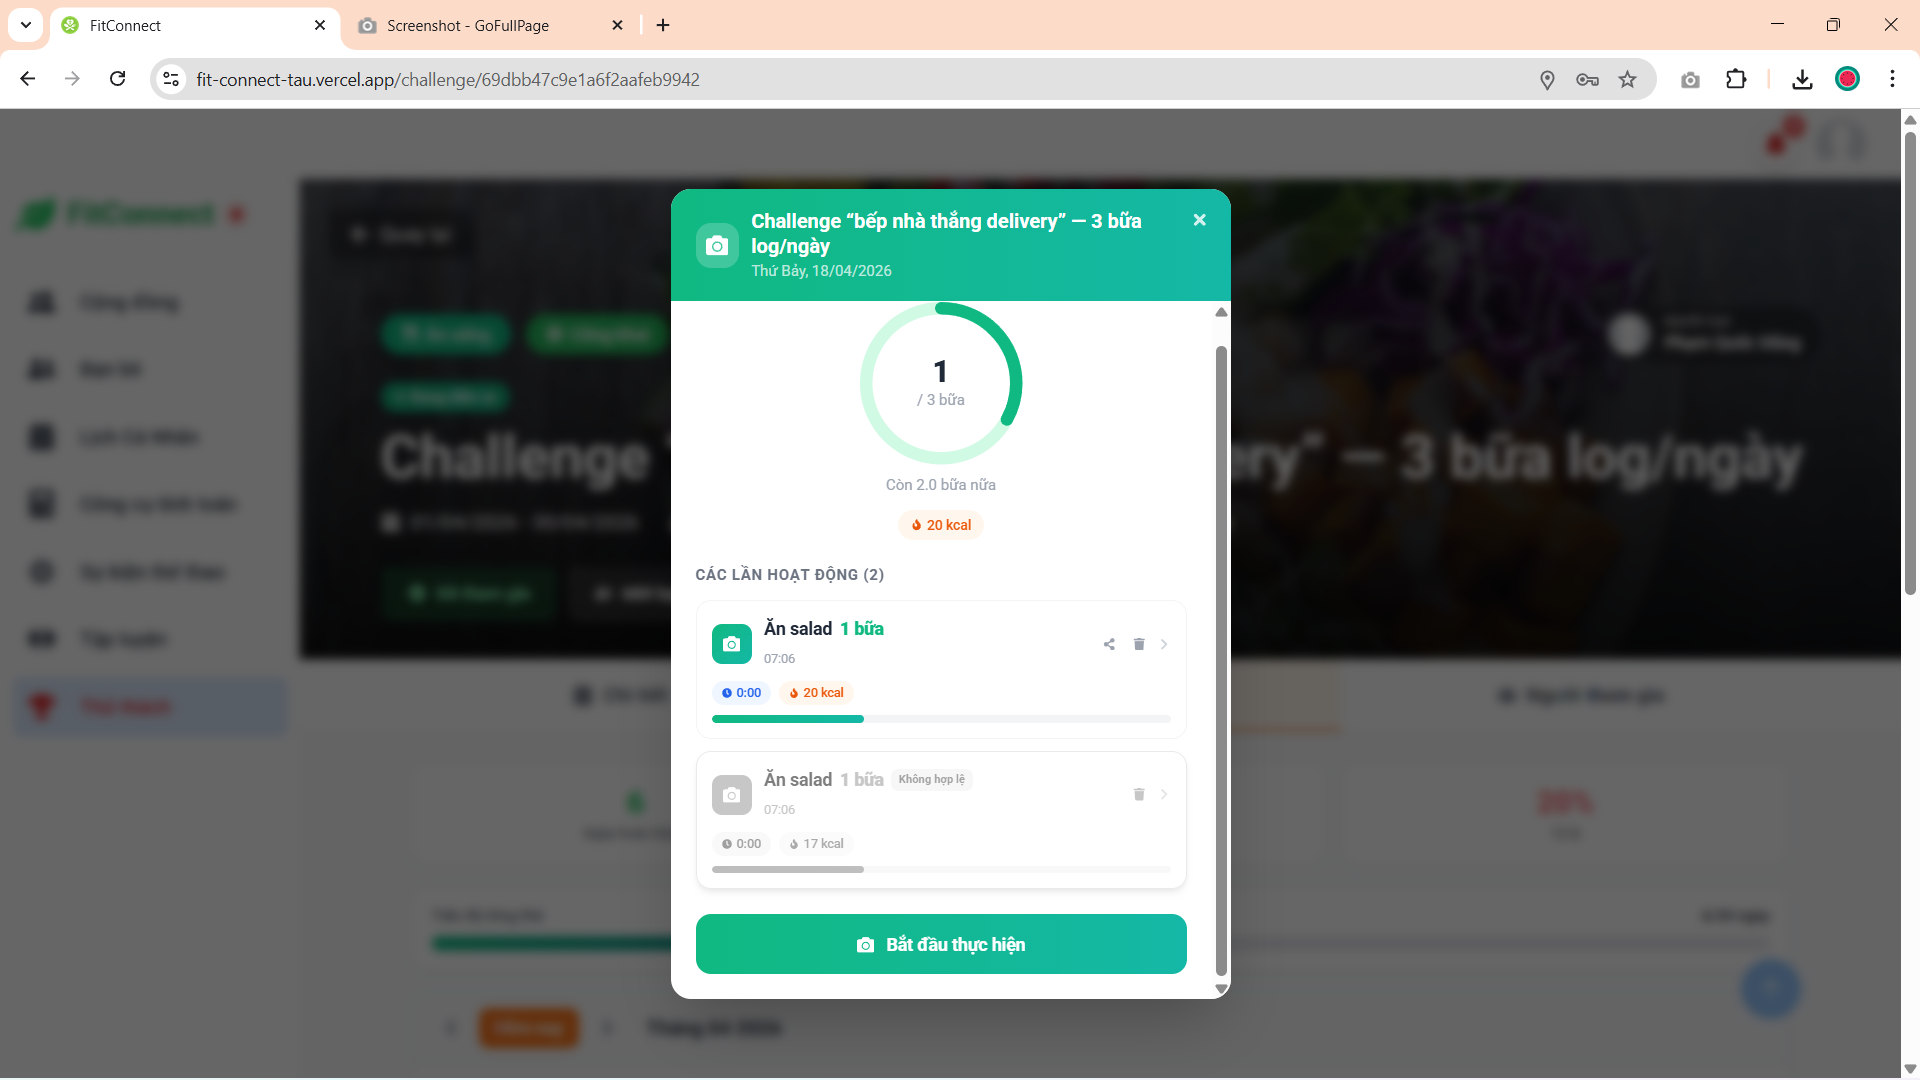
\includegraphics[width=\textwidth]{Images/IMG/nhom4/1modalcapnhatbuaanhople.png}
        \caption{Hệ thống cập nhật tiến độ ngày với bữa ăn hợp lệ}
        \label{fig:impl_ch_food_progress_valid}
    \end{subfigure}
    \hfill
    \begin{subfigure}[b]{0.47\textwidth}
        \centering
        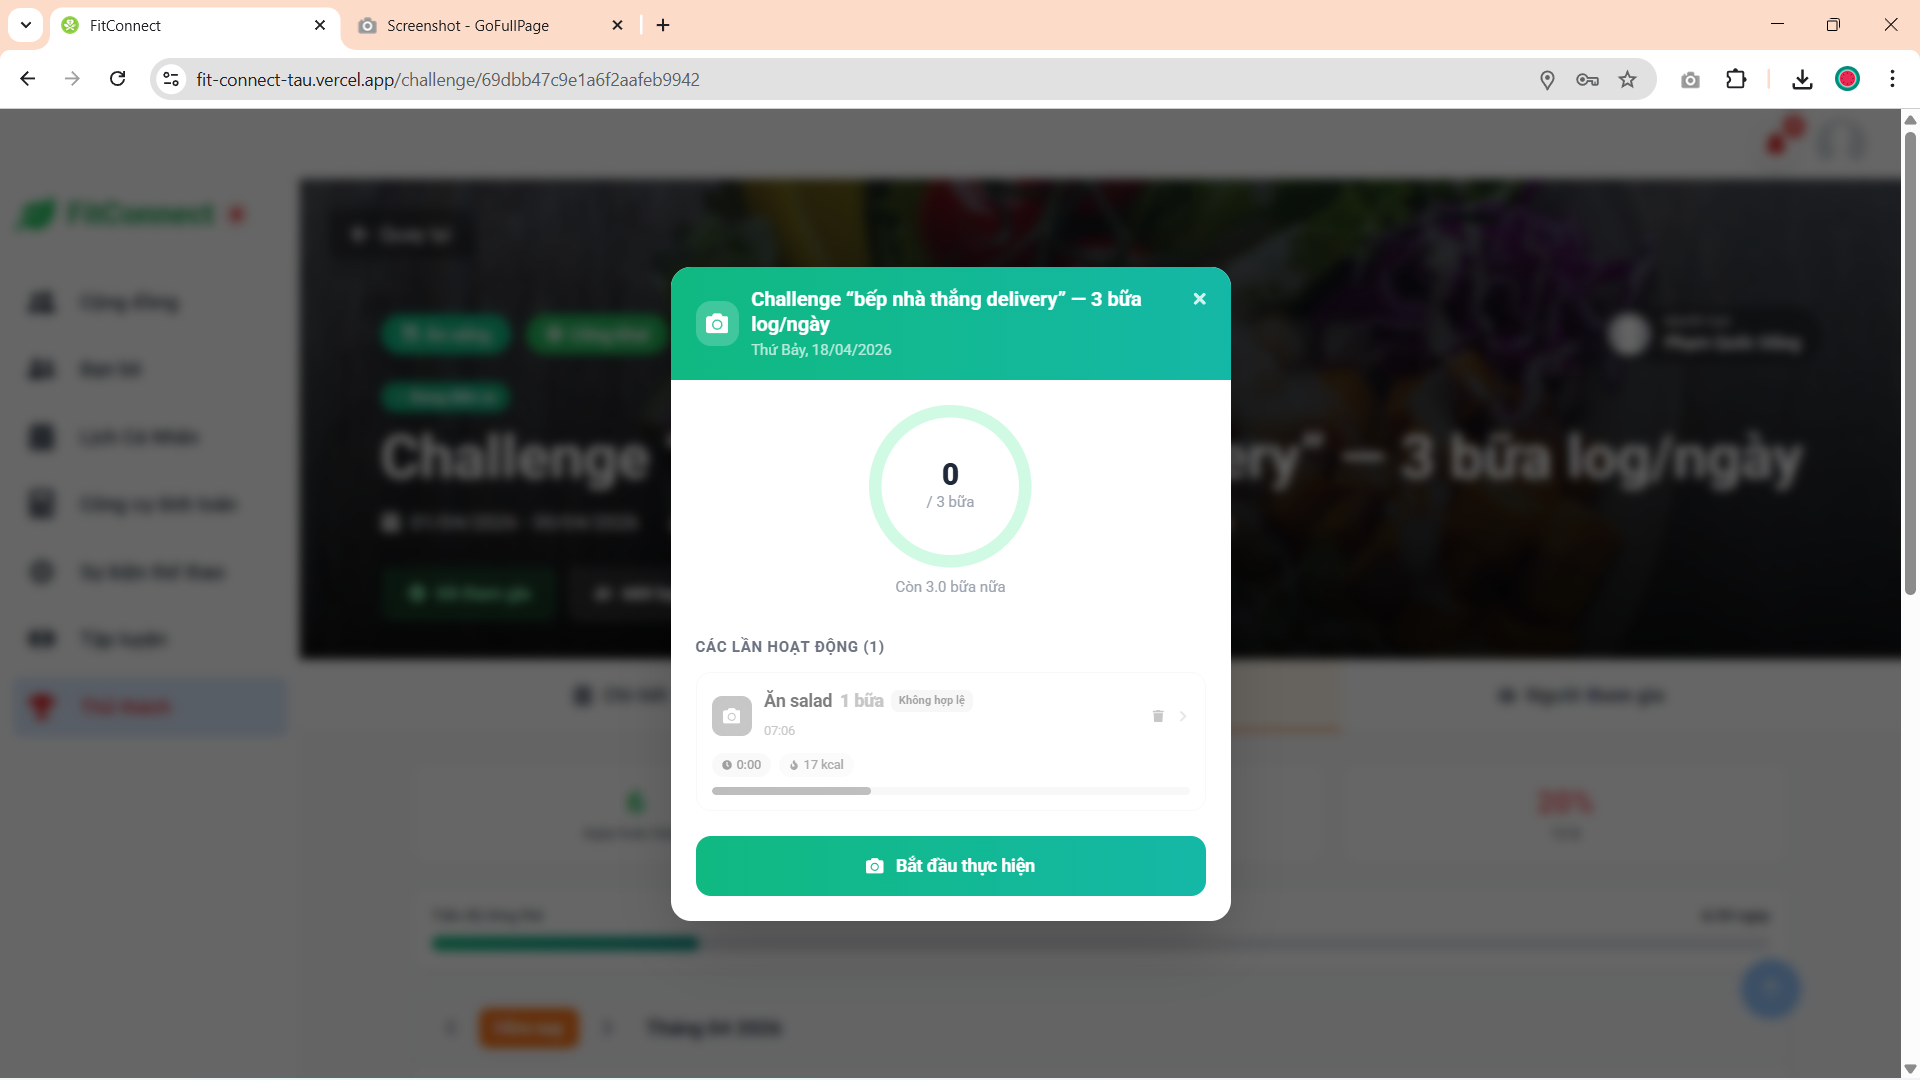
\includegraphics[width=\textwidth]{Images/IMG/nhom4/1tiendokhcapnhatbuaankhhople.png}
        \caption{Hệ thống hiển thị tiến độ khi có bữa ăn không hợp lệ không được tính}
        \label{fig:impl_ch_food_progress_invalid}
    \end{subfigure}
\end{figure}

\end{itemize}

\textbf{c) Đối với thử thách Thể dục (Workout, tập gym,...):}
\begin{itemize}
    \item Người tham gia nhấn vào ngày hiện tại trên lịch tiến độ, hệ thống hiển thị modal bắt đầu thực hiện với thông tin mục tiêu ngày (số bài tập), danh sách bài tập yêu cầu và nút Bắt đầu thực hiện.

\begin{figure}[H]
    \centering
    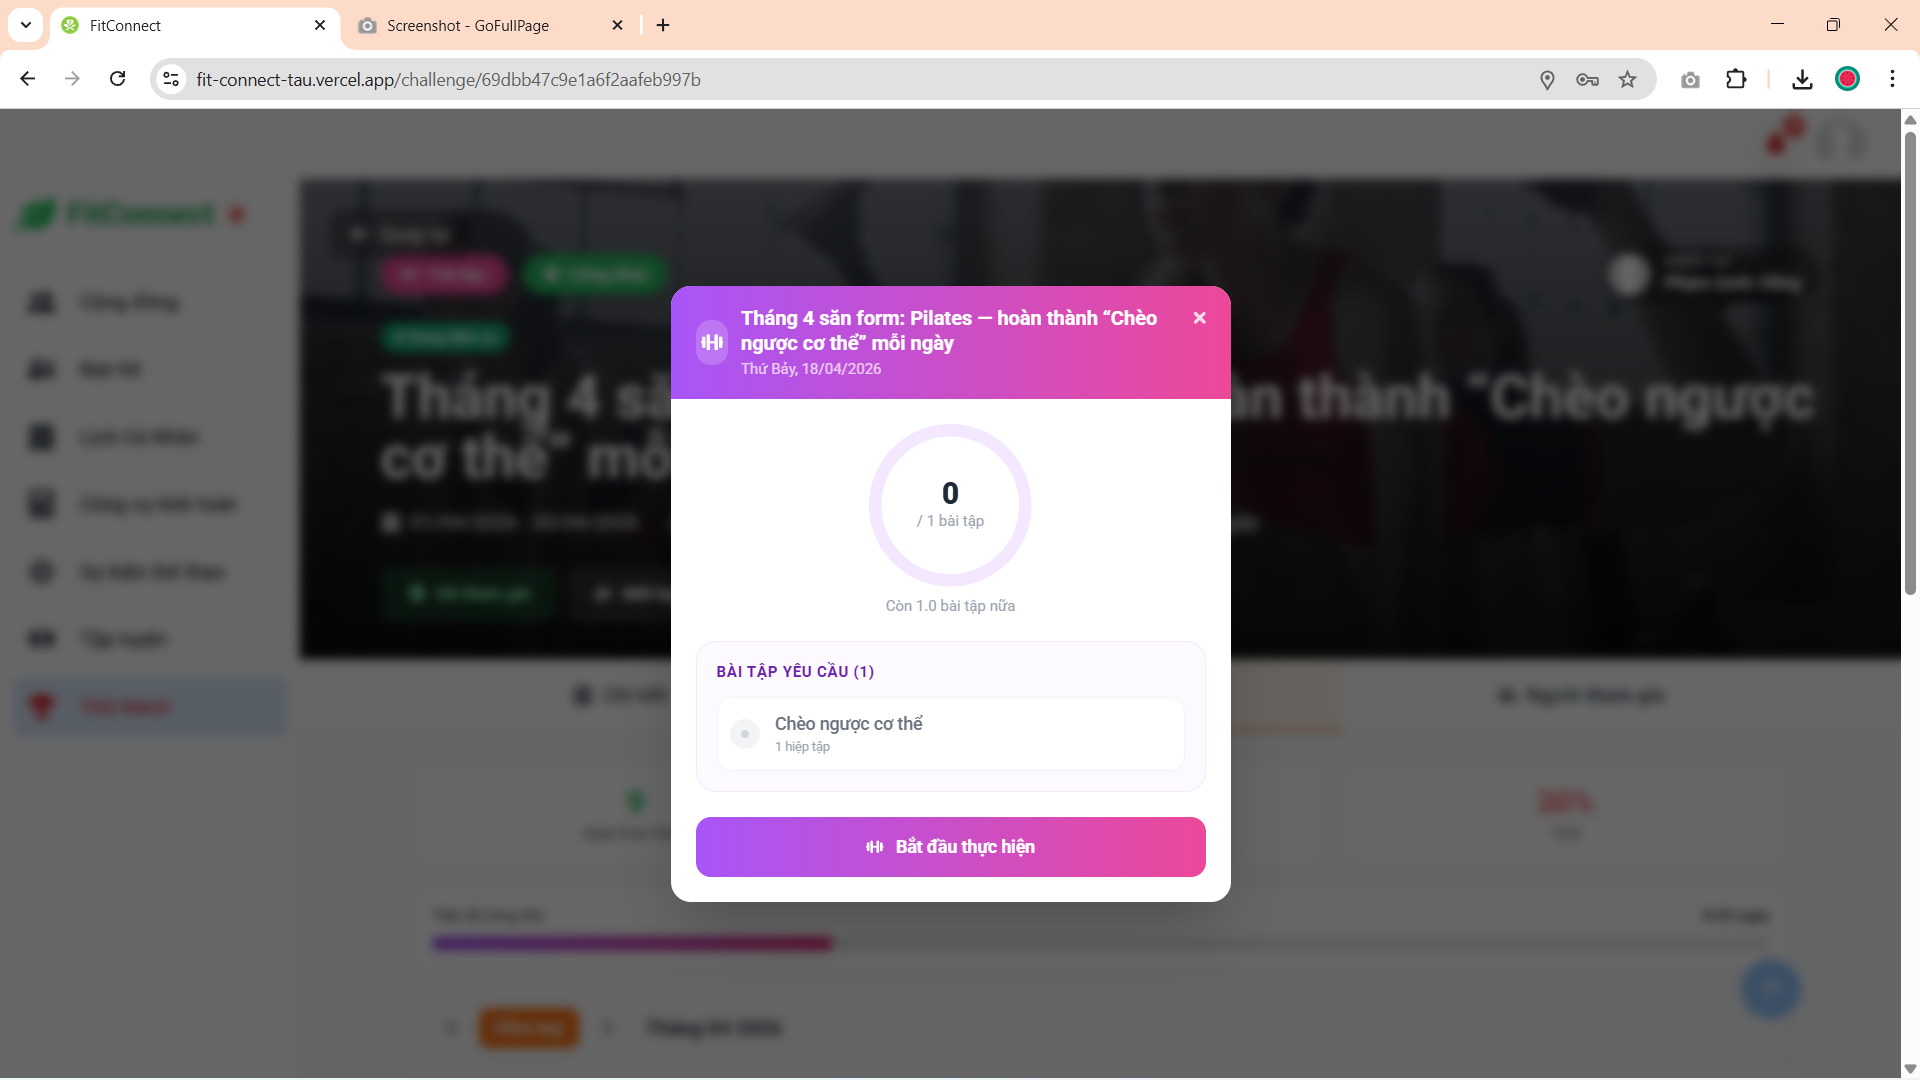
\includegraphics[width=0.60\textwidth]{Images/IMG/nhom4/1modalbatdauthuthachtapluyen.png}
    \caption{Hệ thống hiển thị modal bắt đầu thực hiện thử thách tập luyện}
    \label{fig:impl_ch_exercise_start}
\end{figure}


    \item Khi nhấn Bắt đầu thực hiện, hệ thống chuyển sang trang Chuẩn bị tập luyện gồm 2 bước: Bước 1 -- Chuẩn bị (chỉnh sửa set tập, số lần, mức tạ, kcal cho từng bài tập); Bước 2 -- Tập luyện (thực hiện và theo dõi tiến độ).

\begin{figure}[H]
    \centering
    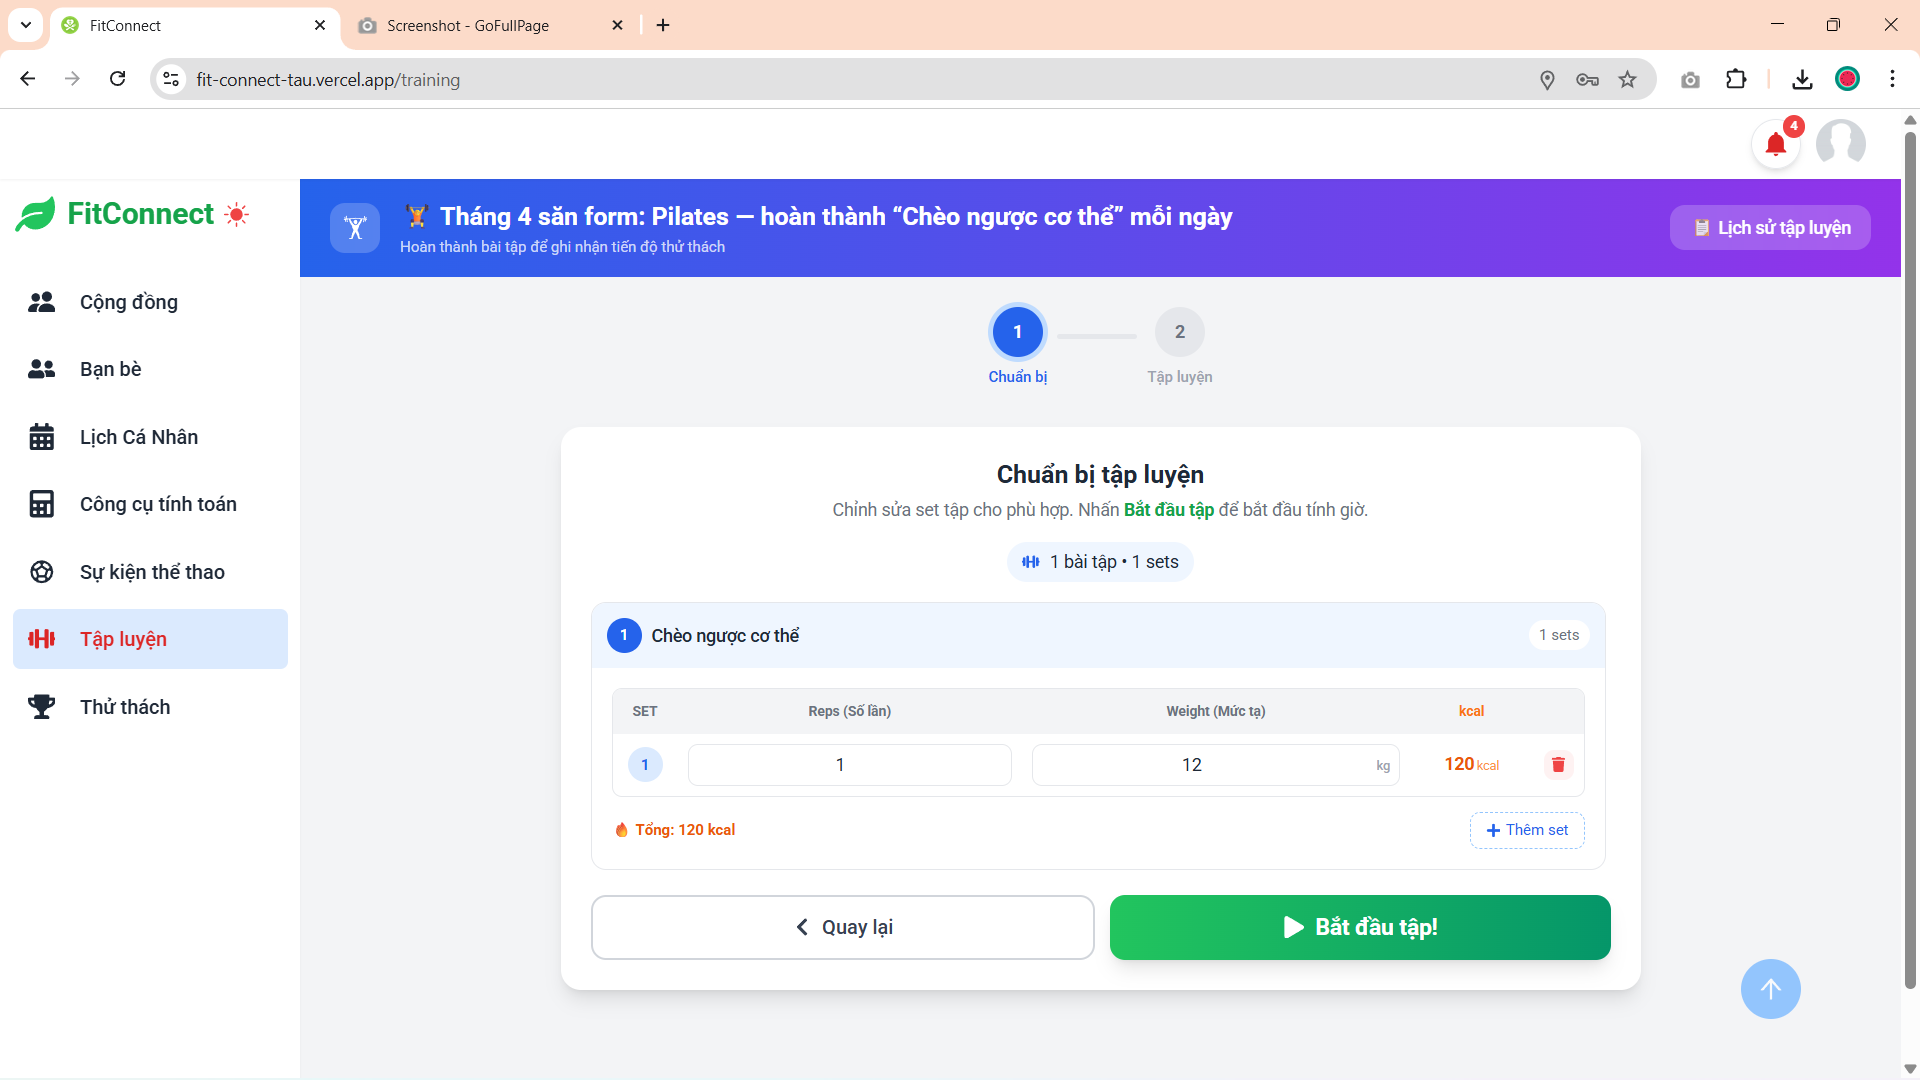
\includegraphics[width=0.60\textwidth]{Images/IMG/nhom4/1chuyenquatrangchuanbitapluyen.png}
    \caption{Người tham gia chuẩn bị tập luyện -- chỉnh sửa set tập}
    \label{fig:impl_ch_exercise_prep}
\end{figure}


    \item Sau khi nhấn Bắt đầu tập, hệ thống chuyển sang bước Tập luyện hiển thị bộ đếm thời gian, số bài tập hoàn thành, kcal đã đốt, và chi tiết từng bài tập (số lần, mức tạ, kcal). Người tham gia đánh dấu hoàn thành từng set và nhấn Hoàn thành tập luyện khi xong.

\begin{figure}[H]
    \centering
    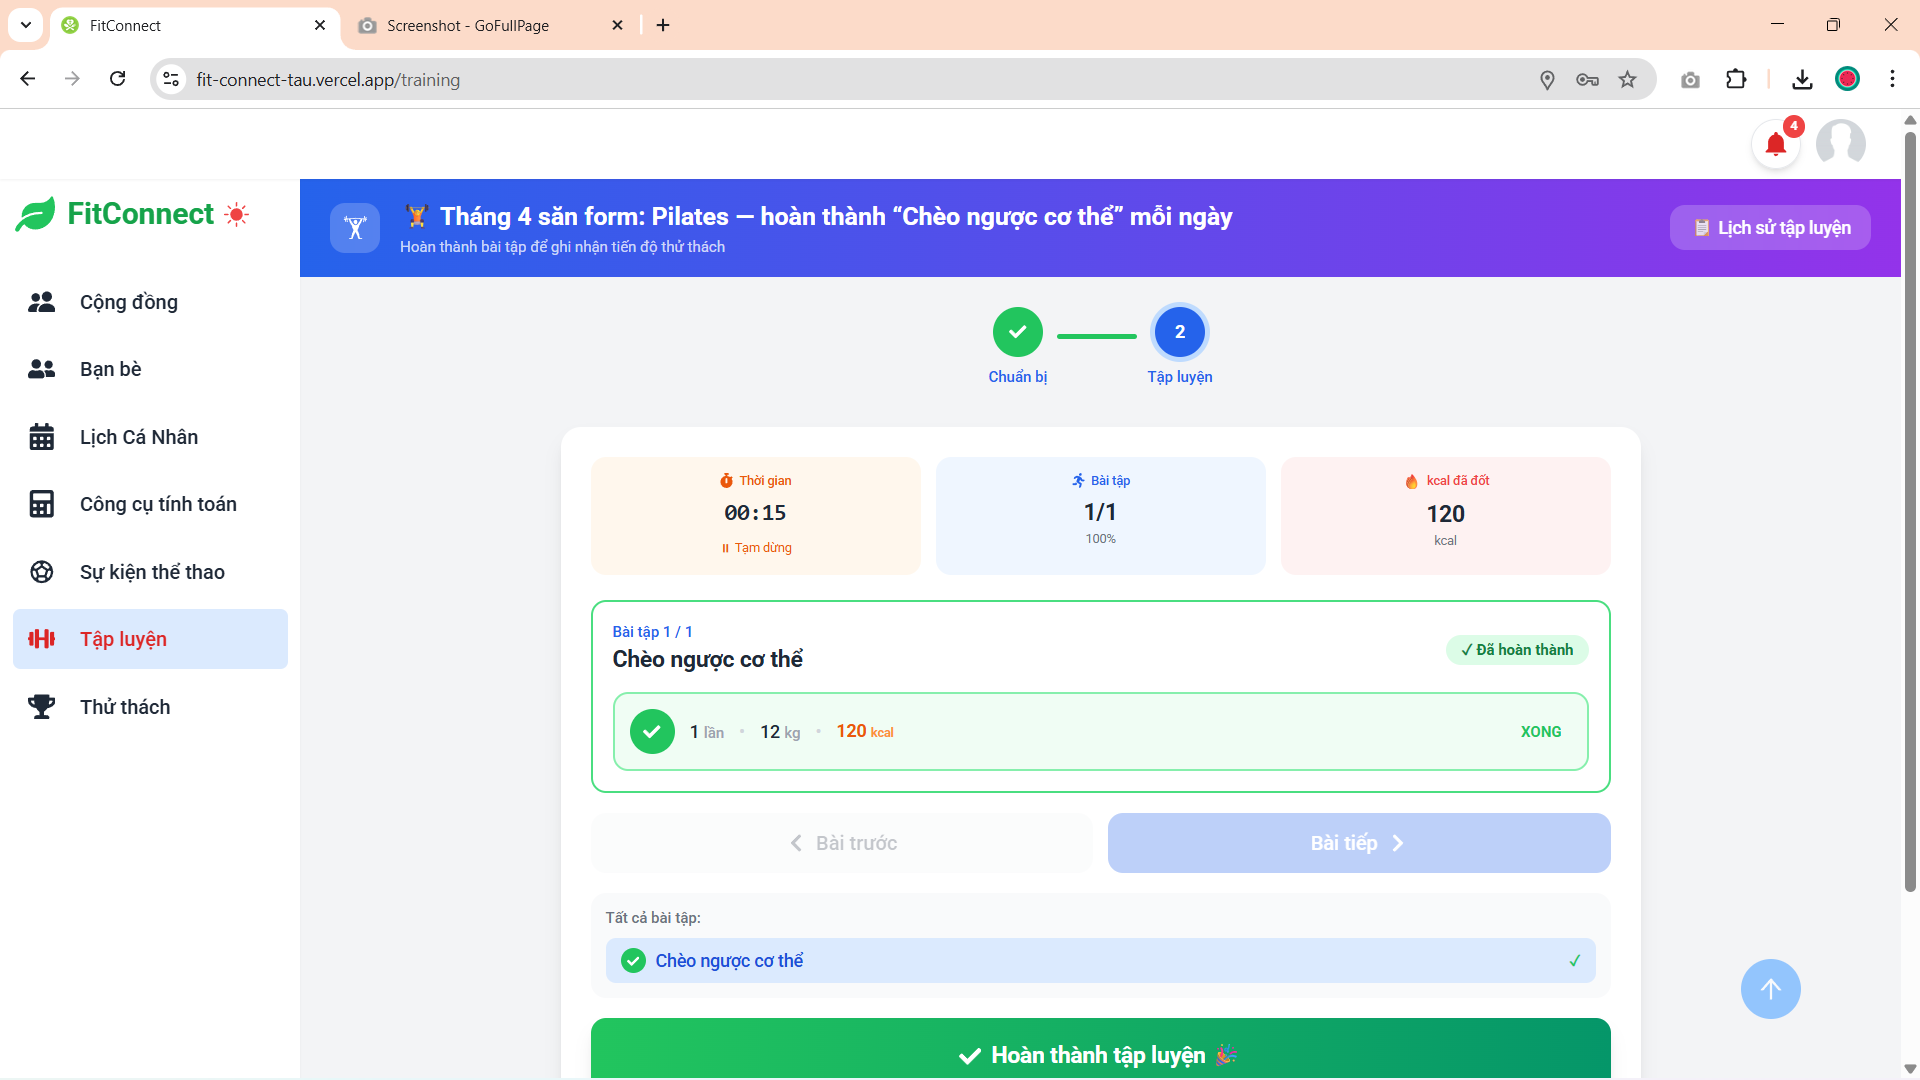
\includegraphics[width=0.60\textwidth]{Images/IMG/nhom4/1chuyenquabuoctapluyen.png}
    \caption{Người tham gia thực hiện tập luyện và theo dõi tiến độ}
    \label{fig:impl_ch_exercise_training}
\end{figure}


    \item Sau khi hoàn thành tập luyện, hệ thống quay lại modal tiến độ ngày hiển thị trạng thái ``Hoàn thành!'' với tổng hợp: thời gian, kcal đốt, danh sách bài tập đã xong và lịch sử các lần hoạt động trong ngày.

\end{itemize}

\textbf{Chia sẻ hoạt động thử thách:}
\begin{itemize}
    \item Người tham gia có thể chia sẻ hoạt động thử thách (tiến độ GPS, kết quả chạy bộ) lên trang Cộng đồng; hoạt động sẽ tự động xuất hiện dưới dạng bài viết trên Bảng tin kèm bản đồ lộ trình.

\begin{figure}[H]
    \centering
    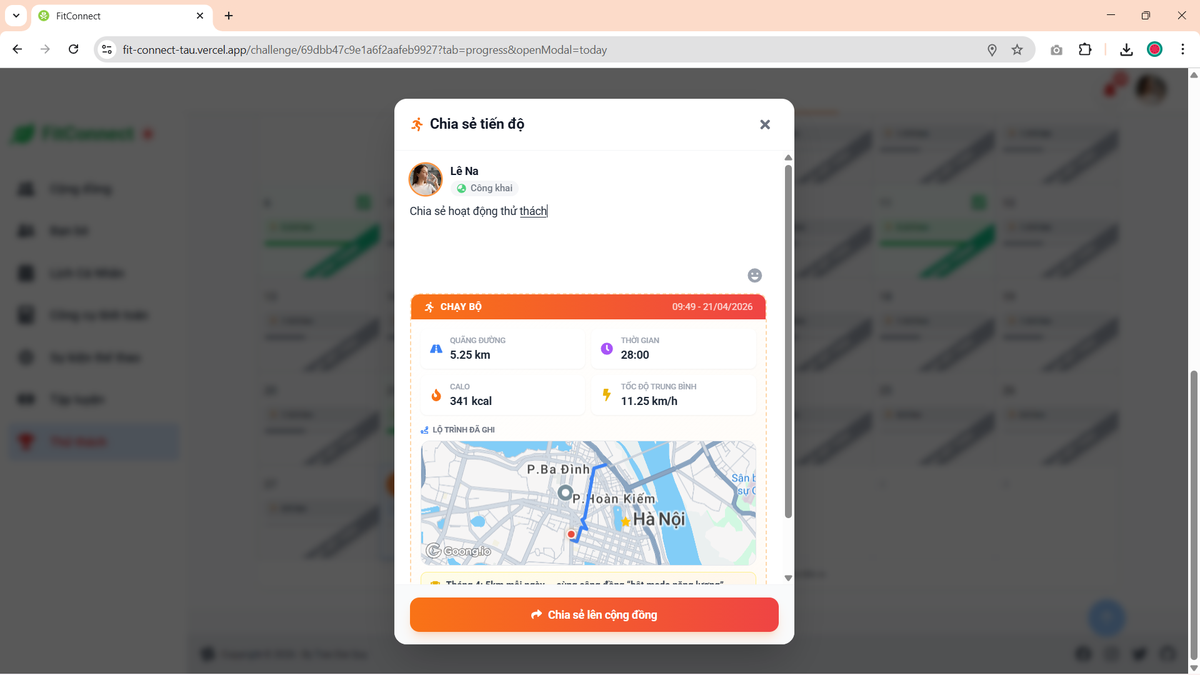
\includegraphics[width=0.60\textwidth]{Images/IMG/nhom4/chiasehoatdongthuthach.png}
    \caption{Người tham gia thao tác chia sẻ hoạt động thử thách lên cộng đồng}
    \label{fig:impl_ch_share_activity}
\end{figure}

\end{itemize}

\subsubsection{Luồng thao tác quản trị thử thách (Góc độ Quản trị viên)}
\begin{itemize}
    \item Quản trị viên truy cập trang Kiểm duyệt thử thách, hệ thống hiển thị danh sách thử thách bị báo cáo bao gồm thông tin: người tạo thử thách, tên thử thách, số báo cáo, người báo cáo, nội dung báo cáo và các hành động (xem chi tiết, giữ thử thách, gỡ thử thách).

\begin{figure}[H]
    \centering
    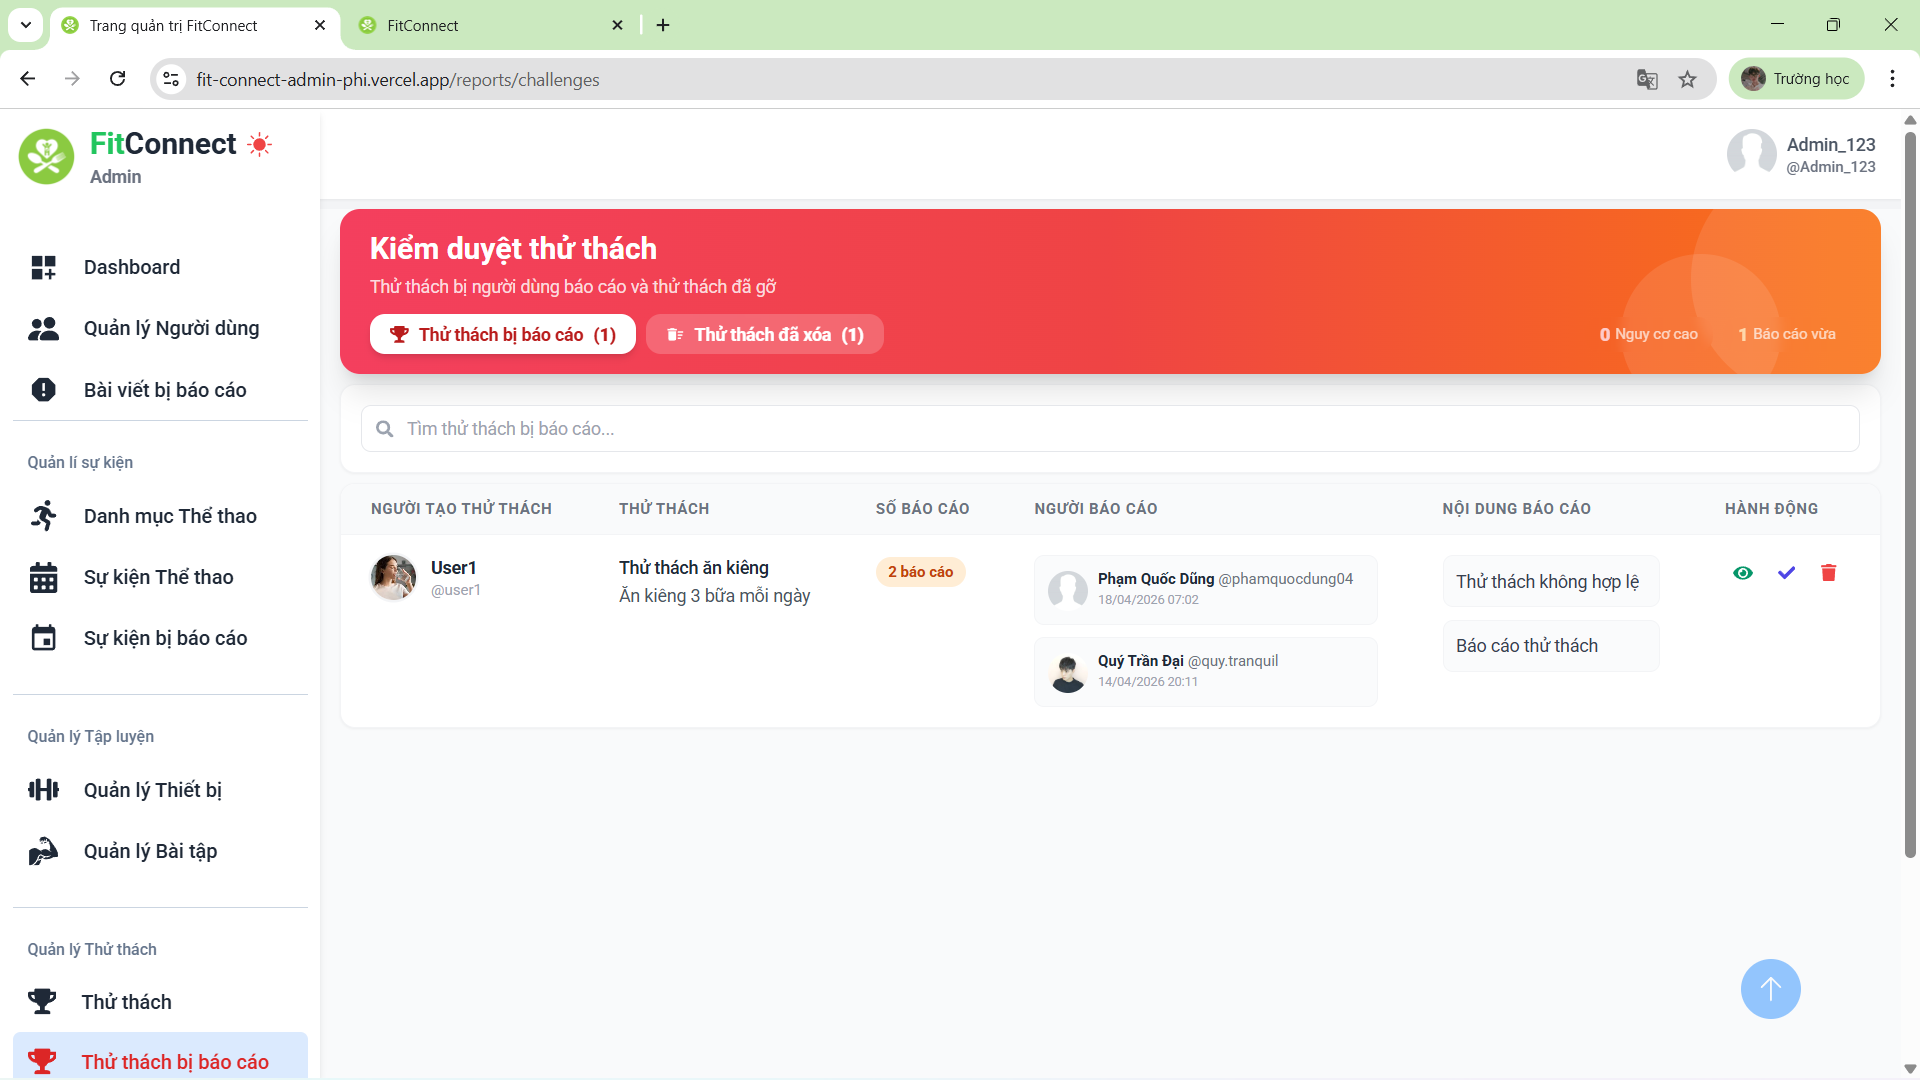
\includegraphics[width=0.60\textwidth]{Images/IMG/nhom4/adminxemthuthachbibaocao.png}
    \caption{Quản trị viên xem danh sách thử thách bị báo cáo}
    \label{fig:impl_ch_admin_list}
\end{figure}


    \item Quản trị viên có thể nhấn xem chi tiết để xem thông tin thử thách bị báo cáo bao gồm: tên thử thách, trạng thái, thời gian diễn ra, số người tham gia, danh sách người báo cáo và thông tin chi tiết thử thách.

\begin{figure}[H]
    \centering
    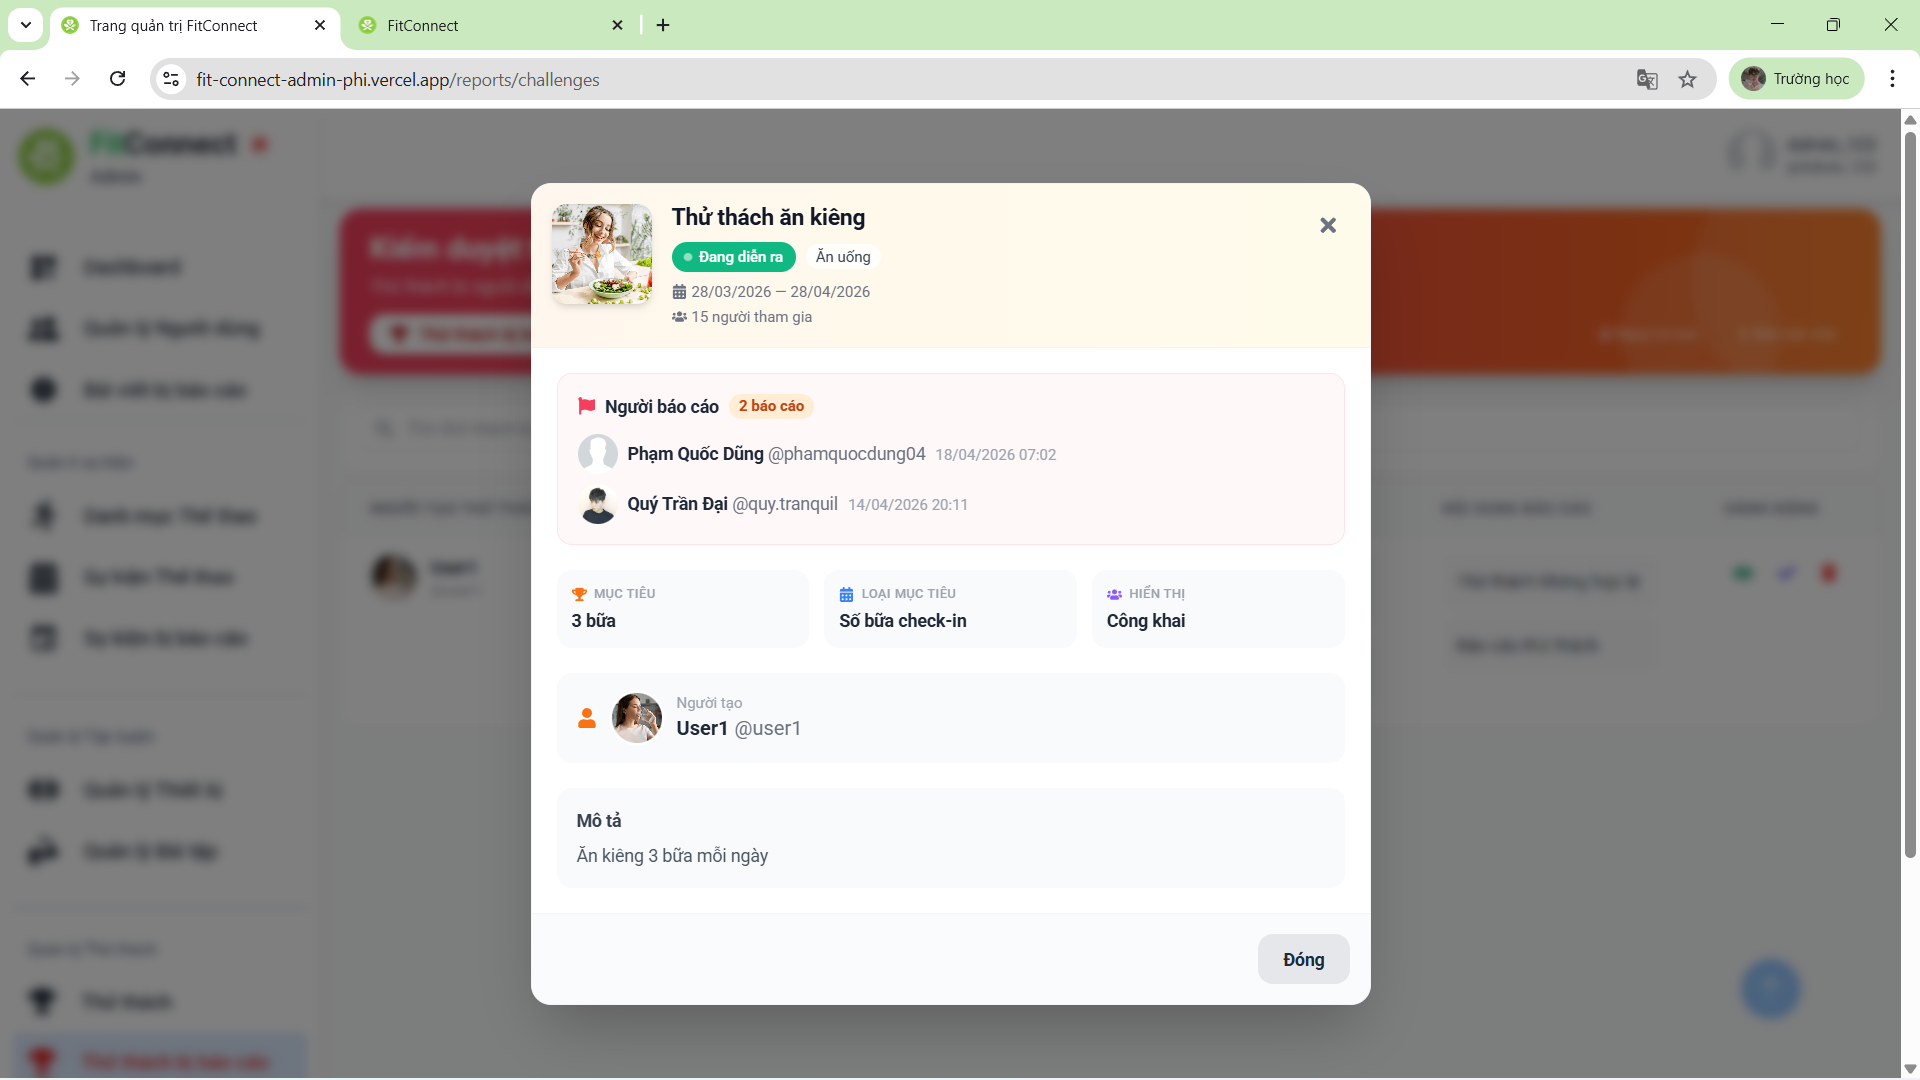
\includegraphics[width=0.60\textwidth]{Images/IMG/nhom4/adminxemthongtinthuthachbaoca.png}
    \caption{Quản trị viên xem thông tin chi tiết thử thách bị báo cáo}
    \label{fig:impl_ch_admin_view}
\end{figure}


    \item Quản trị viên xử lý thử thách bị báo cáo theo hai hướng: \textbf{Giữ lại} (thử thách tiếp tục hiển thị bình thường) hoặc \textbf{Gỡ} (thử thách bị ẩn và chuyển vào danh sách đã xóa). Tại tab ``Đã xóa'', Quản trị viên có thể xem xét và khôi phục thử thách nếu cần.

\begin{figure}[H]
    \centering
    \begin{subfigure}[b]{0.47\textwidth}
        \centering
        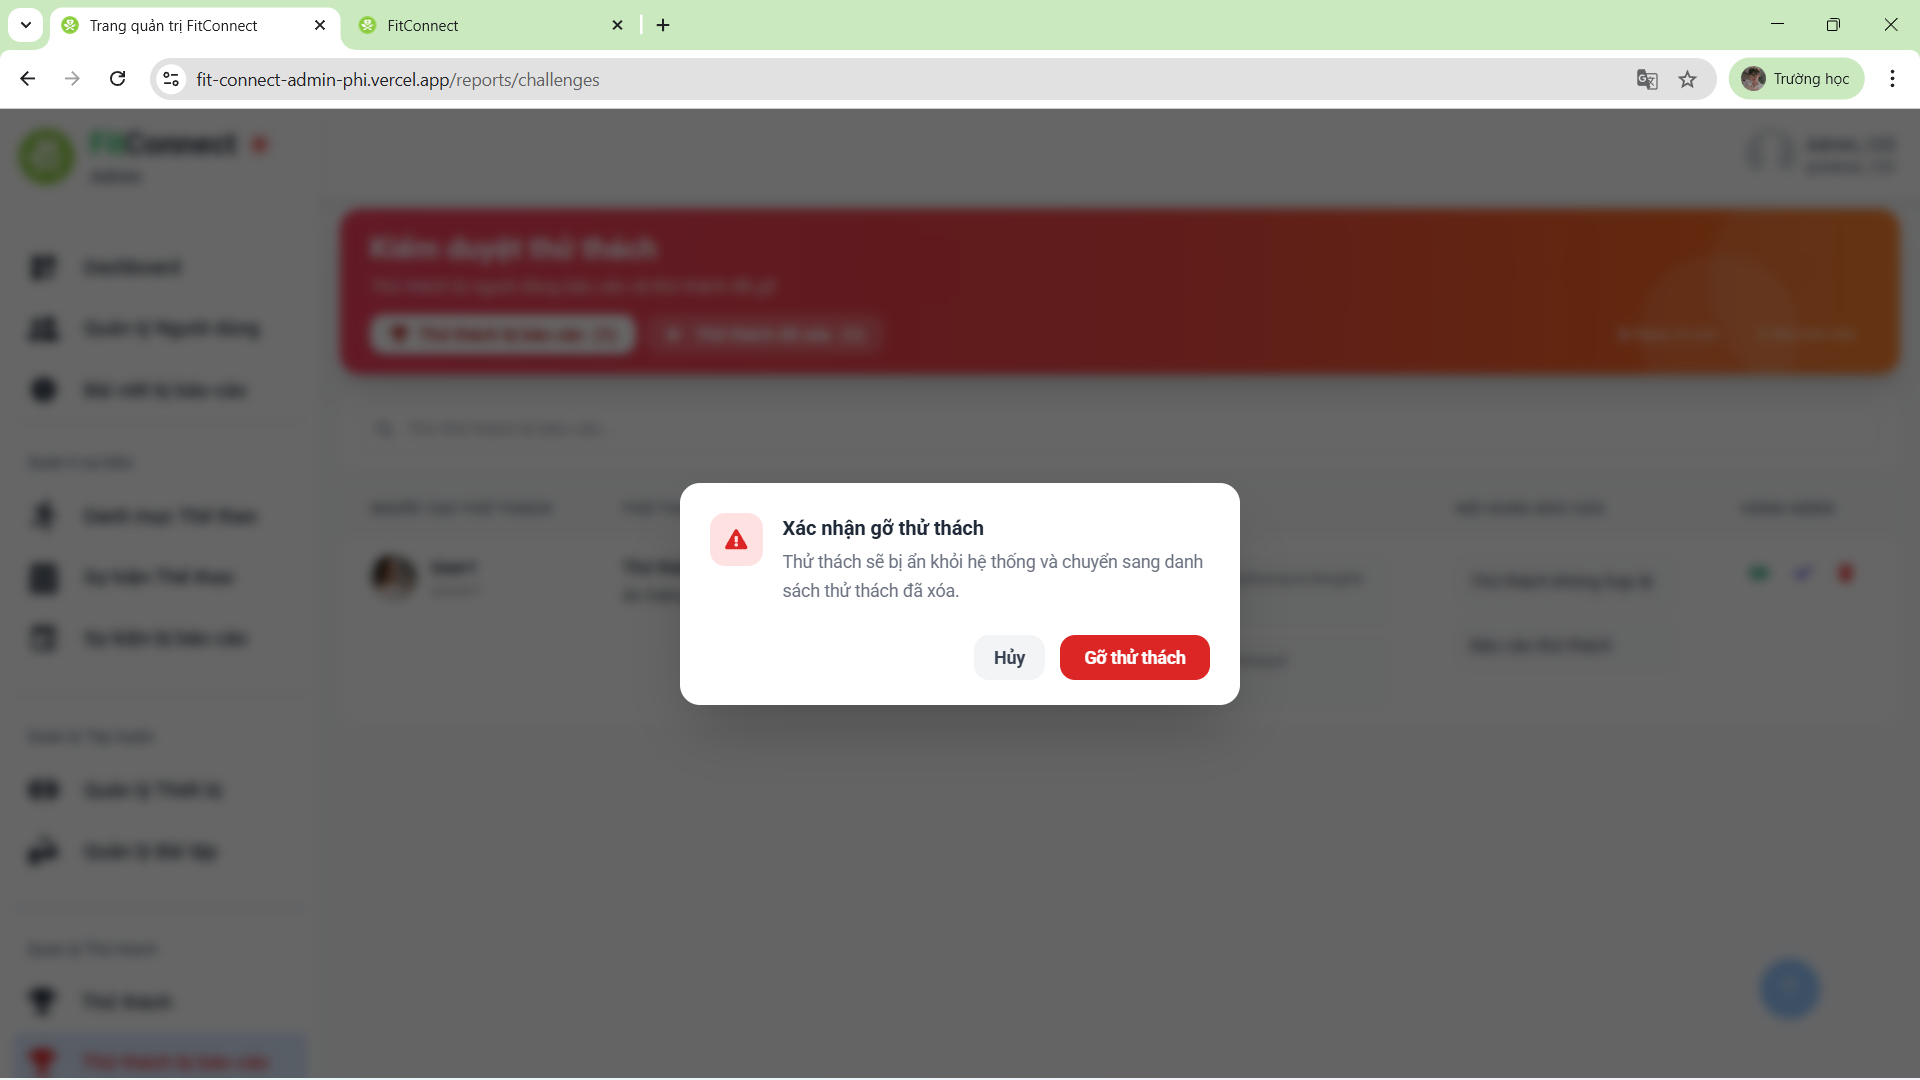
\includegraphics[width=\textwidth]{Images/IMG/nhom4/adminxoathuthach.png}
        \caption{Gỡ thử thách vi phạm khỏi cộng đồng}
        \label{fig:impl_ch_admin_delete}
    \end{subfigure}
    \hfill
    \begin{subfigure}[b]{0.47\textwidth}
        \centering
        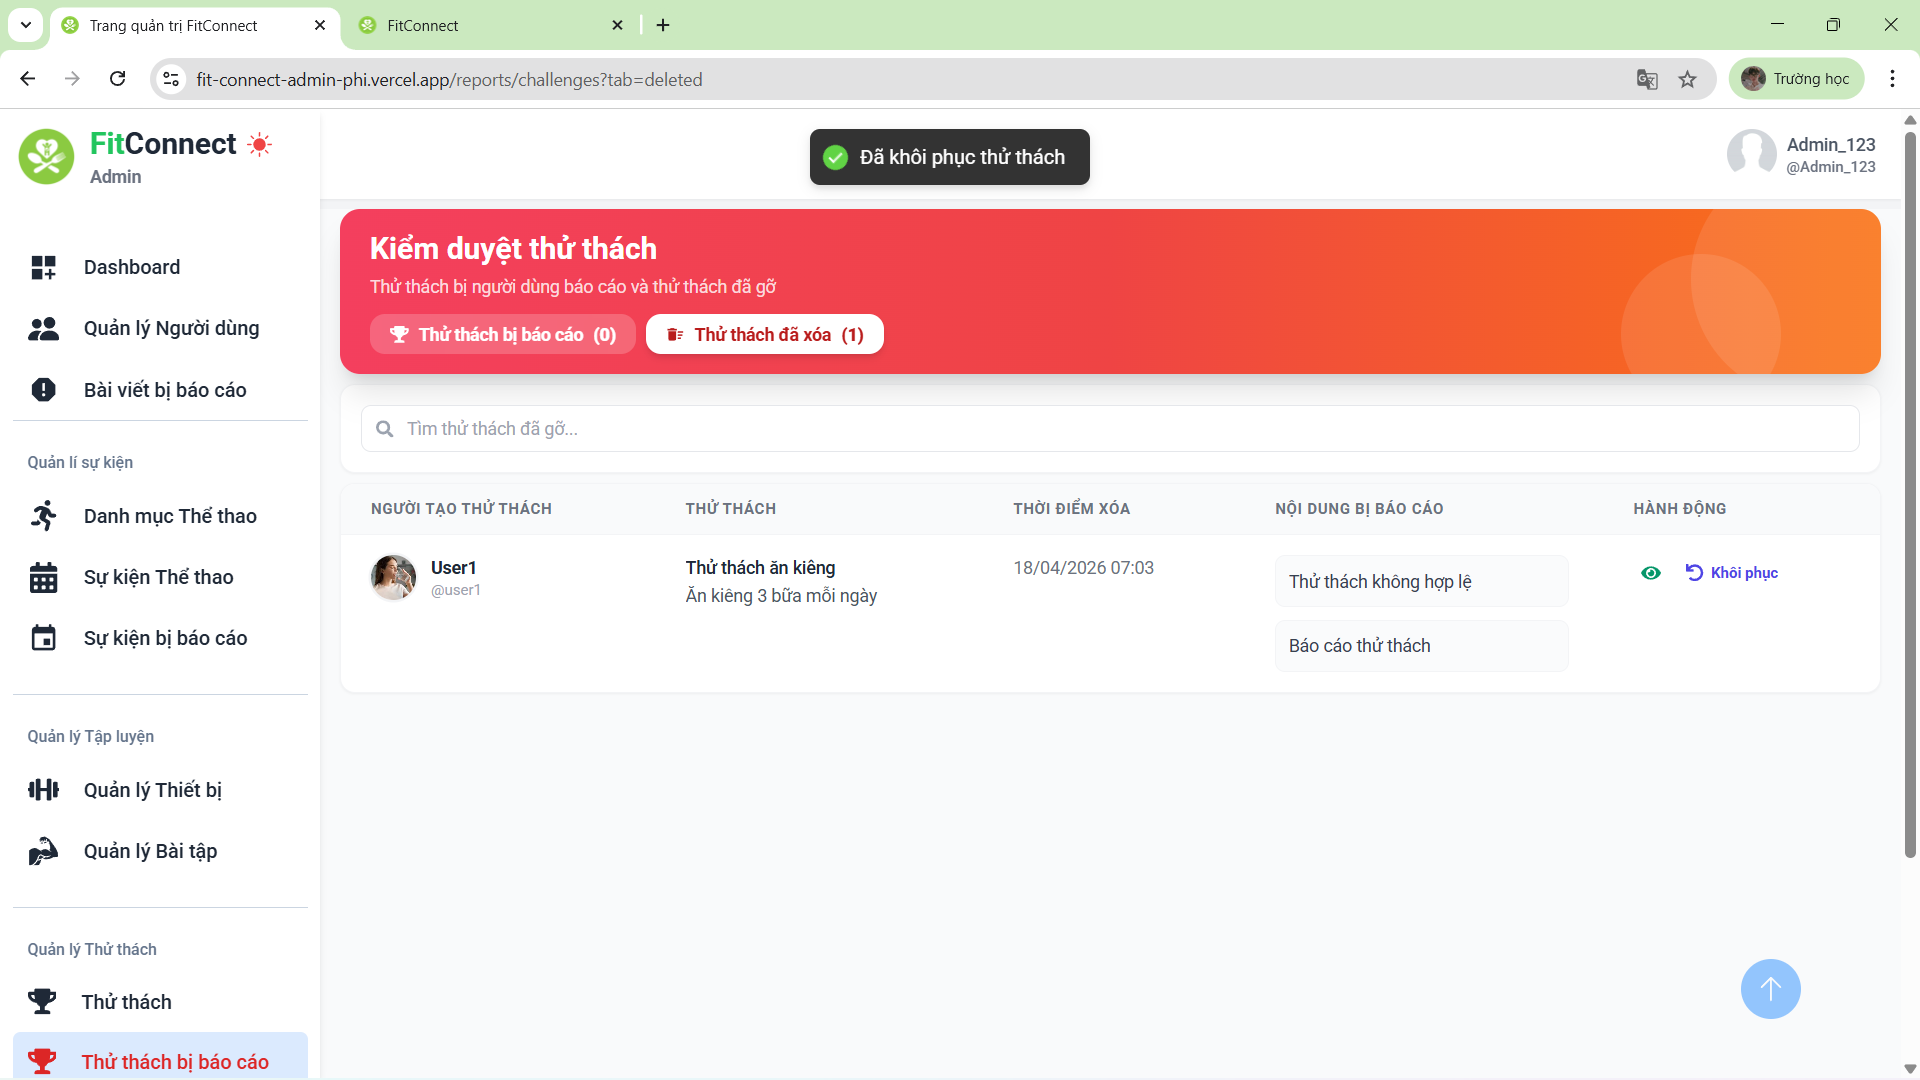
\includegraphics[width=\textwidth]{Images/IMG/nhom4/adminxemthuthachdaxoa.png}
        \caption{Danh sách thử thách đã xóa và tùy chọn khôi phục}
        \label{fig:impl_ch_admin_deleted_list}
    \end{subfigure}
    \vspace{0.3em}
    \caption{Quản trị viên xử lý và quản lý thử thách vi phạm}
    \label{fig:impl_ch_admin_moderation}
\end{figure}

\end{itemize}

\subsection{Nhóm tính năng Tính toán chỉ số sức khỏe}
\label{subsec:impl_health_calculator}

Nhóm tính năng Tính toán chỉ số sức khỏe cung cấp cho người dùng bộ công cụ toàn diện để đo lường, theo dõi và phân tích các chỉ số thể chất cá nhân. Hệ thống hỗ trợ 8 công cụ tính toán: BMI (Body Mass Index -- Chỉ số khối cơ thể), TDEE (Total Daily Energy Expenditure -- Tổng năng lượng tiêu thụ mỗi ngày), Body Fat (Phần trăm mỡ cơ thể), BMR (Basal Metabolic Rate -- Tỷ lệ trao đổi chất cơ bản), IBW (Ideal Body Weight -- Cân nặng lý tưởng), LBM (Lean Body Mass -- Khối lượng cơ nạc), Calories Burned (Lượng calories đốt cháy) và Water Need (Nhu cầu nước hàng ngày). Điểm nổi bật của hệ thống là sự tích hợp AI để phân tích sức khỏe và gợi ý bài tập phù hợp ngay từ kết quả tính toán, đồng thời lưu trữ lịch sử chỉ số để người dùng theo dõi sự thay đổi theo thời gian.

\subsubsection{Luồng tính toán và phân tích chỉ số sức khỏe}

\begin{itemize}
    \item Người dùng truy cập trang Công cụ tính toán từ thanh điều hướng bên trái. Hệ thống hiển thị giao diện trang tính toán gồm 2 tab: ``Công cụ tính'' và ``Lịch sử chỉ số''. Tại tab Công cụ tính, hệ thống hiển thị danh sách 8 công cụ tính toán sức khỏe, mỗi công cụ gồm tên viết tắt, tên đầy đủ, mô tả ngắn gọn và nút ``Tính ngay''.

\begin{figure}[H]
    \centering
    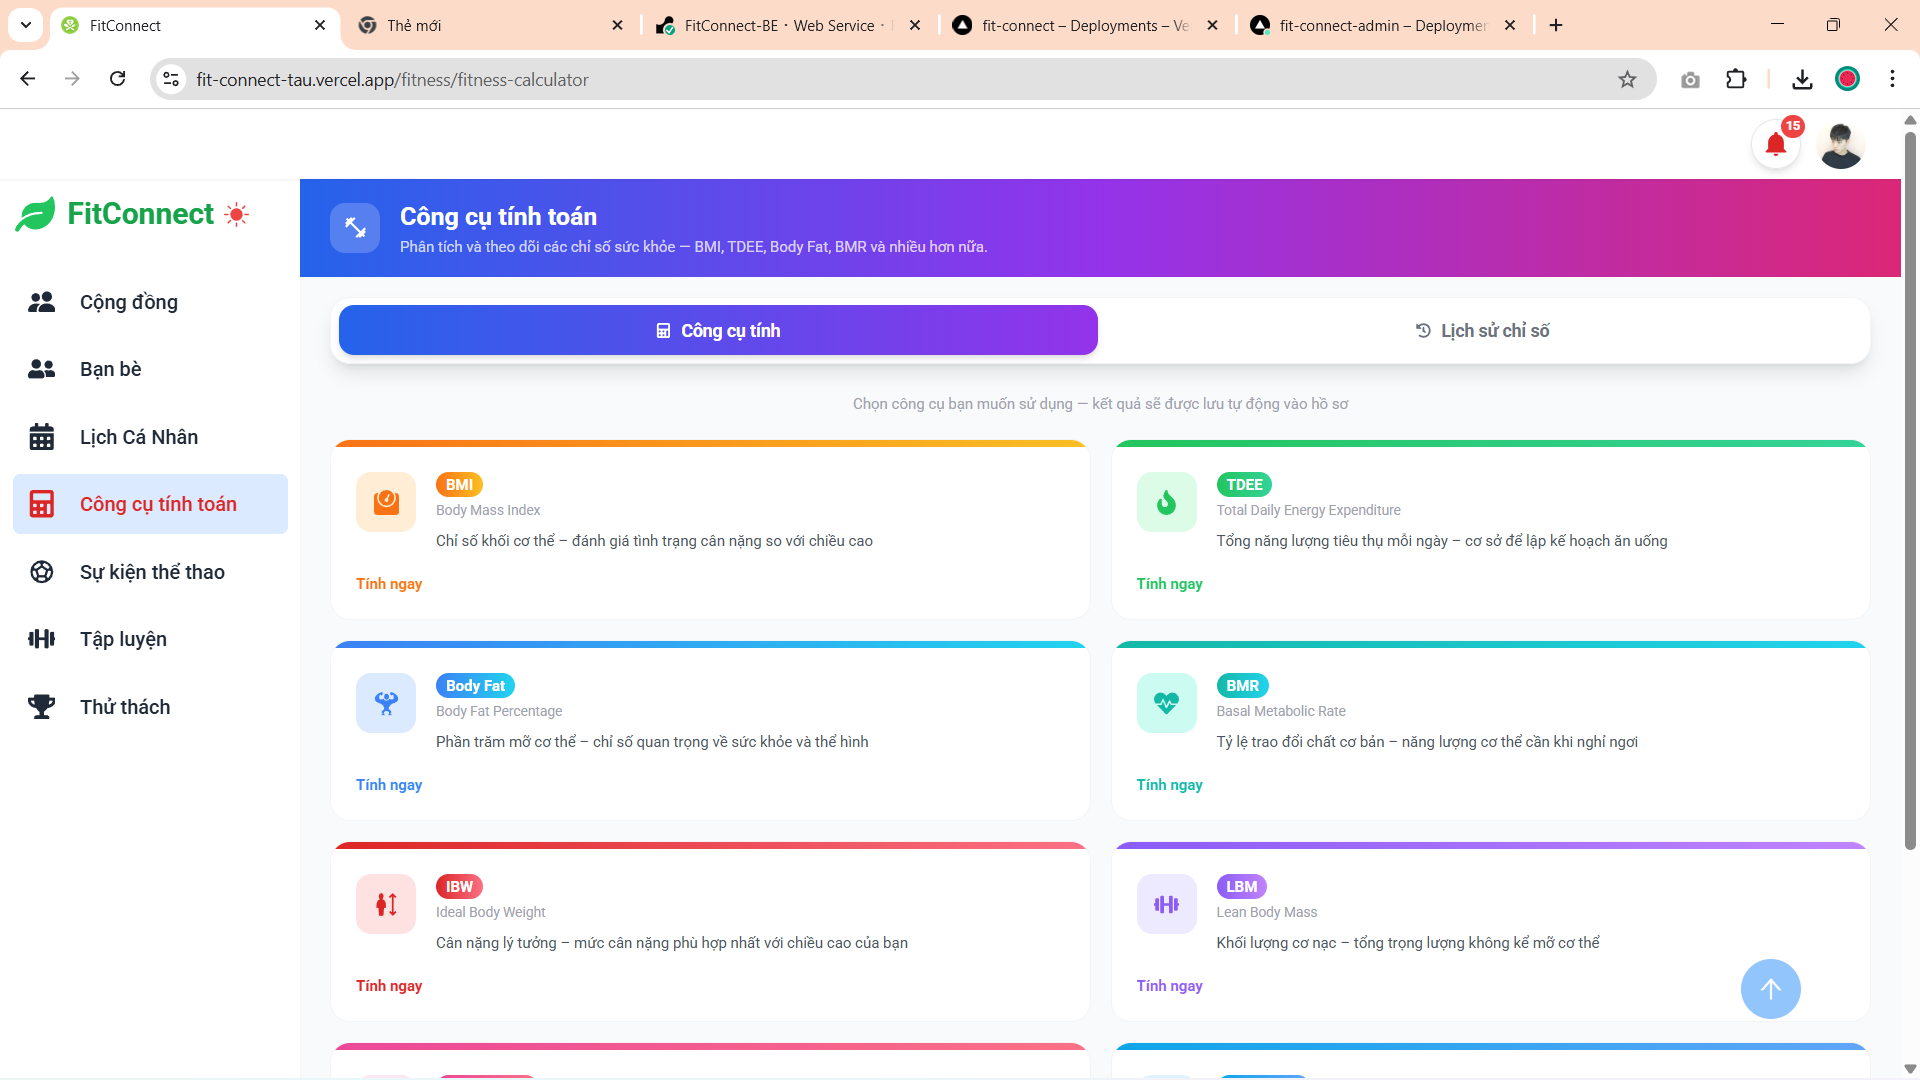
\includegraphics[width=0.60\textwidth]{Images/IMG/nhom6/giaodientrangtinhtoanchiso.png}
    \caption{Hệ thống hiển thị trang Công cụ tính toán chỉ số sức khỏe}
    \label{fig:impl_calc_main}
\end{figure}


    \item Người dùng nhấn ``Tính ngay'' vào một công cụ (ví dụ: BMI), hệ thống chuyển đến trang tính toán chi tiết của chỉ số đó. Tại đây, hệ thống hiển thị bài viết giải thích chi tiết về chỉ số (định nghĩa, công thức, ý nghĩa), biểu mẫu nhập dữ liệu (chiều cao, cân nặng, tuổi, giới tính tùy theo loại chỉ số) và kết quả tính toán kèm đánh giá trực quan (thanh màu phân vùng, phân loại tình trạng). Kết quả sau khi tính được tự động lưu vào hồ sơ cá nhân của người dùng.

    \item Sau khi có kết quả, người dùng có thể nhấn nút ``AI Phân Tích Sức Khỏe''. Hệ thống gửi các chỉ số sức khỏe hiện tại tới AI, AI phân tích và trả về modal hiển thị: phần ``Đánh giá sức khỏe'' với nhận xét chi tiết về tình trạng sức khỏe dựa trên chỉ số, và phần ``Bài tập được gợi ý'' với danh sách các bài tập phù hợp từ kho bài tập hệ thống kèm nhãn mức độ (Dễ, Trung bình), loại bài tập (Sức mạnh, Cardio) và lý do AI gợi ý cho từng bài.

\begin{figure}[H]
    \centering
    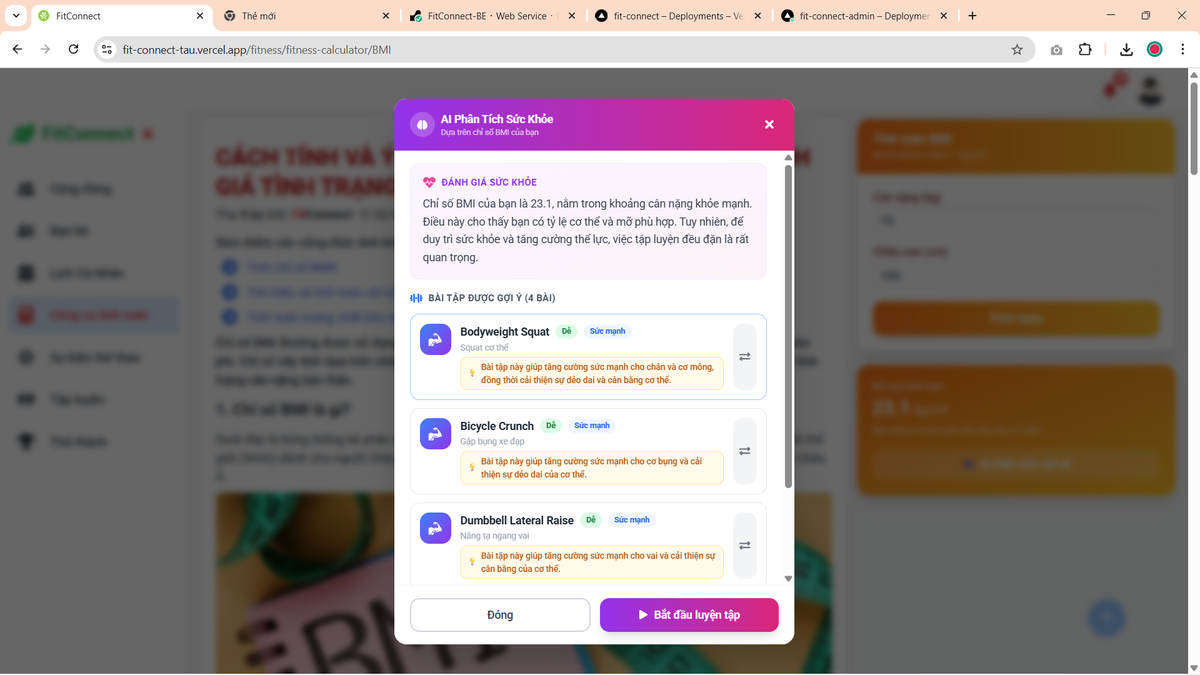
\includegraphics[width=0.60\textwidth]{Images/IMG/nhom6/AIphantichsuckhoa.png}
    \caption{Hệ thống AI phân tích sức khỏe và gợi ý bài tập dựa trên chỉ số BMI}
    \label{fig:impl_calc_ai}
\end{figure}


    \item Người dùng có thể chọn các bài tập gợi ý và nhấn ``Bắt đầu luyện tập''. Hệ thống chuyển sang trang Chuẩn bị tập luyện hiển thị danh sách các bài tập đã chọn (ví dụ: 4 bài tập, 5 sets), cho phép người dùng chỉnh sửa số lần (Reps), mức tạ (Weight), thêm set trước khi bắt đầu. Hệ thống tự động tính kcal ước tính cho mỗi set. Người dùng cũng có thể nhấn ``Lưu bài tập'' để lưu giáo án tập luyện cho lần sau.

\begin{figure}[H]
    \centering
    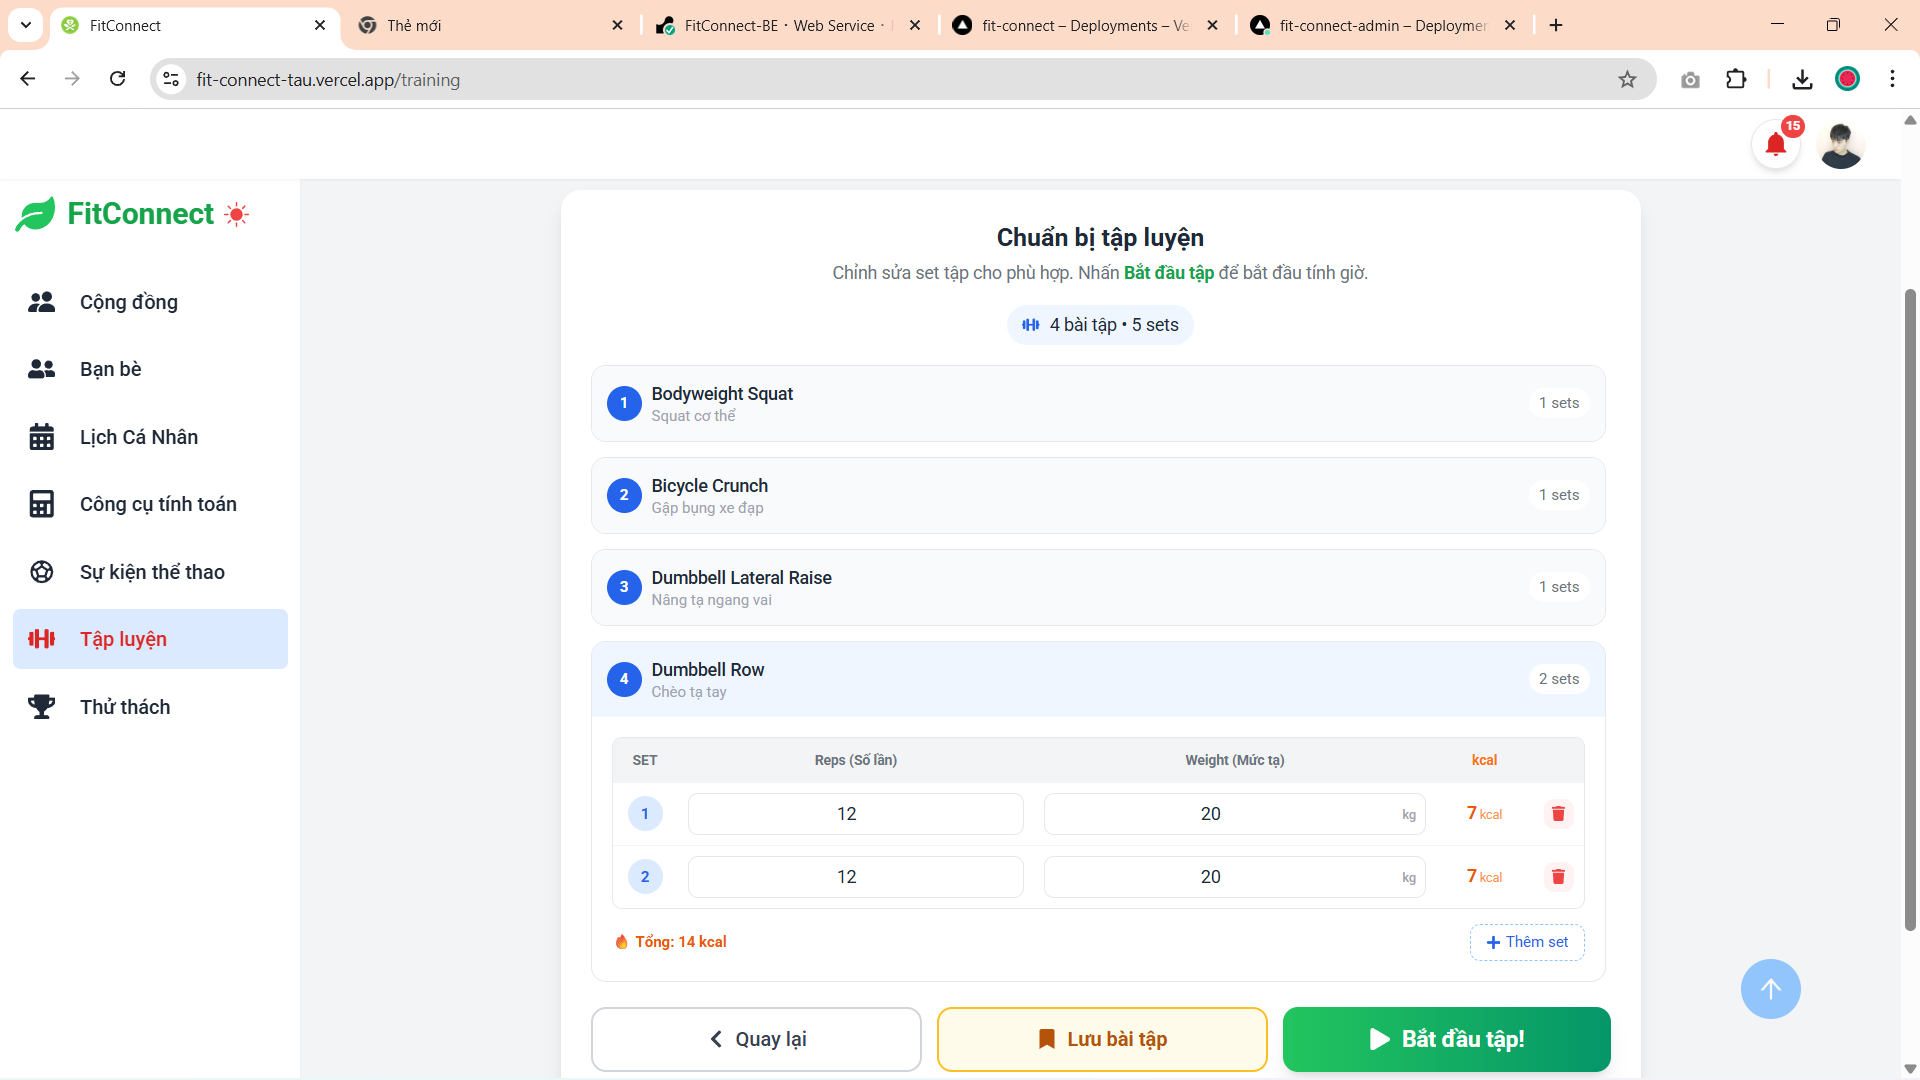
\includegraphics[width=0.60\textwidth]{Images/IMG/nhom6/chuyenquamanchuanbitapluyen.png}
    \caption{Người dùng chuẩn bị tập luyện với các bài tập được AI gợi ý}
    \label{fig:impl_calc_prep}
\end{figure}


    \item Khi nhấn ``Bắt đầu tập!'', hệ thống chuyển sang trang Tập luyện hiển thị bộ đếm thời gian thực, số bài tập hoàn thành (ví dụ: 0/4), kcal đã đốt, và chi tiết từng bài tập với thông tin set (số lần, mức tạ, kcal). Người dùng đánh dấu ``Xong'' cho từng set sau khi hoàn thành và nhấn ``Bài tiếp'' để chuyển sang bài tập tiếp theo.

\begin{figure}[H]
    \centering
    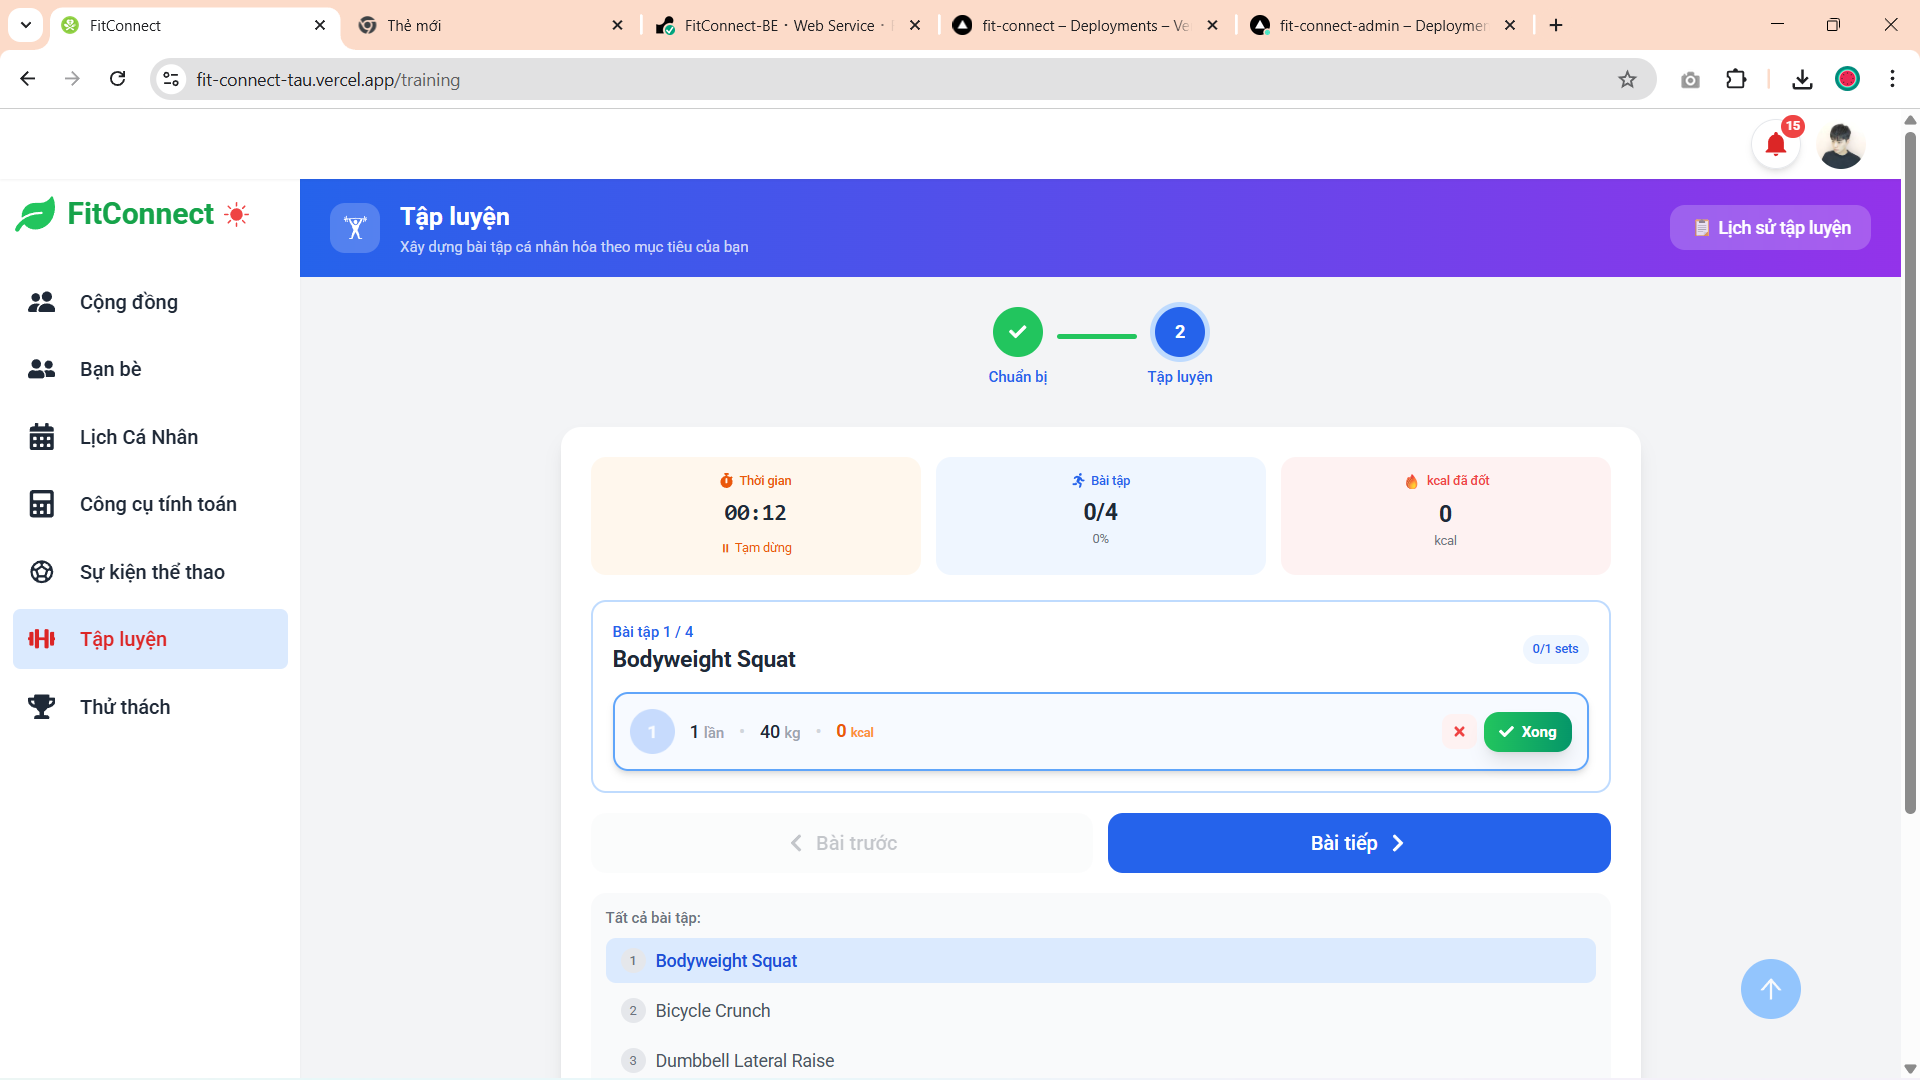
\includegraphics[width=0.60\textwidth]{Images/IMG/nhom6/batdautapluyen.png}
    \caption{Người dùng thực hiện tập luyện và theo dõi tiến độ từng bài tập}
    \label{fig:impl_calc_training}
\end{figure}


    \item Sau khi hoàn thành tất cả bài tập, hệ thống đánh dấu xanh toàn bộ danh sách và hiện nút ``Hoàn thành tập luyện''. Khi xác nhận, buổi tập được ghi nhận tự động vào lịch sử tập luyện của người dùng.

\end{itemize}

\subsubsection{Theo dõi lịch sử chỉ số sức khỏe}

\begin{itemize}
    \item Người dùng chuyển sang tab ``Lịch sử chỉ số''. Hệ thống hiển thị tổng quan các chỉ số sức khỏe hiện tại (BMI, BMR, TDEE, Body Fat, LBM, IBW) dưới dạng thẻ tóm tắt ở đầu trang. Bên dưới, hệ thống hiển thị biểu đồ theo dõi theo thời gian cho từng chỉ số: Cân nặng (kg), BMI (kg/m²), BMR (kcal), TDEE (kcal/ngày), Body Fat (\%), LBM (kg) và IBW (kg). Mỗi biểu đồ có nút ``Cập nhật'' để người dùng cập nhật chỉ số mới nhất.

    \item Người dùng có thể lọc dữ liệu biểu đồ theo các khoảng thời gian: 1 ngày, 7 ngày, 1 tháng, 6 tháng, Tất cả, hoặc Tùy chọn (chọn ngày cụ thể). Hệ thống cũng hiển thị phần ``Chỉ số chưa có'' kèm nút tính nhanh để người dùng bổ sung các chỉ số còn thiếu.

\begin{figure}[H]
    \centering
    
\includegraphics[width=0.60\textwidth]{Images/IMG/nhom6/lichsuchiso.png}
    \caption{Hệ thống hiển thị lịch sử chỉ số sức khỏe với biểu đồ theo thời gian}
    \label{fig:impl_calc_history}
\end{figure}

\end{itemize}

\subsection{Nhóm tính năng Tập luyện}
\label{subsec:impl_training}

Nhóm tính năng Tập luyện là hệ sinh thái xây dựng và thực hiện bài tập cá nhân hóa theo mục tiêu sức khỏe của người dùng. Hệ thống cung cấp 4 chế độ luyện tập đa dạng: \textbf{Tùy chỉnh} (tự chọn thiết bị, nhóm cơ, bài tập), \textbf{AI Gợi ý Tập Luyện} (mô tả tình trạng sức khỏe để AI phân tích và gợi ý bài tập phù hợp), \textbf{Hoạt động ngoài trời} (chạy bộ, đạp xe với theo dõi GPS thời gian thực trên bản đồ), và \textbf{Bài tập đã lưu} (sử dụng lại giáo án đã lưu kèm lịch tập định kỳ). Ngoài ra, hệ thống tích hợp trang Lịch sử tập luyện giúp người dùng theo dõi toàn bộ hoạt động tập luyện theo thời gian.

\subsubsection{Luồng tập luyện Tùy chỉnh}

\begin{itemize}
    \item Người dùng truy cập trang Tập luyện từ thanh điều hướng bên trái. Hệ thống hiển thị giao diện ``Chọn chế độ luyện tập'' với 4 thẻ chế độ: Tùy chỉnh (tự chọn thiết bị, nhóm cơ và bài tập theo ý muốn), AI Gợi ý Tập Luyện (mô tả tình trạng sức khỏe để AI tư vấn và gợi ý bài tập phù hợp), Hoạt động ngoài trời (chạy bộ, đạp xe, ghi hoạt động theo thời gian thực trên bản đồ), và Bài tập đã lưu (sử dụng lại giáo án đã lưu trước đó). Ở góc trên bên phải, hệ thống hiển thị nút ``Lịch sử tập luyện'' để truy cập nhanh lịch sử.

\begin{figure}[H]
    \centering
    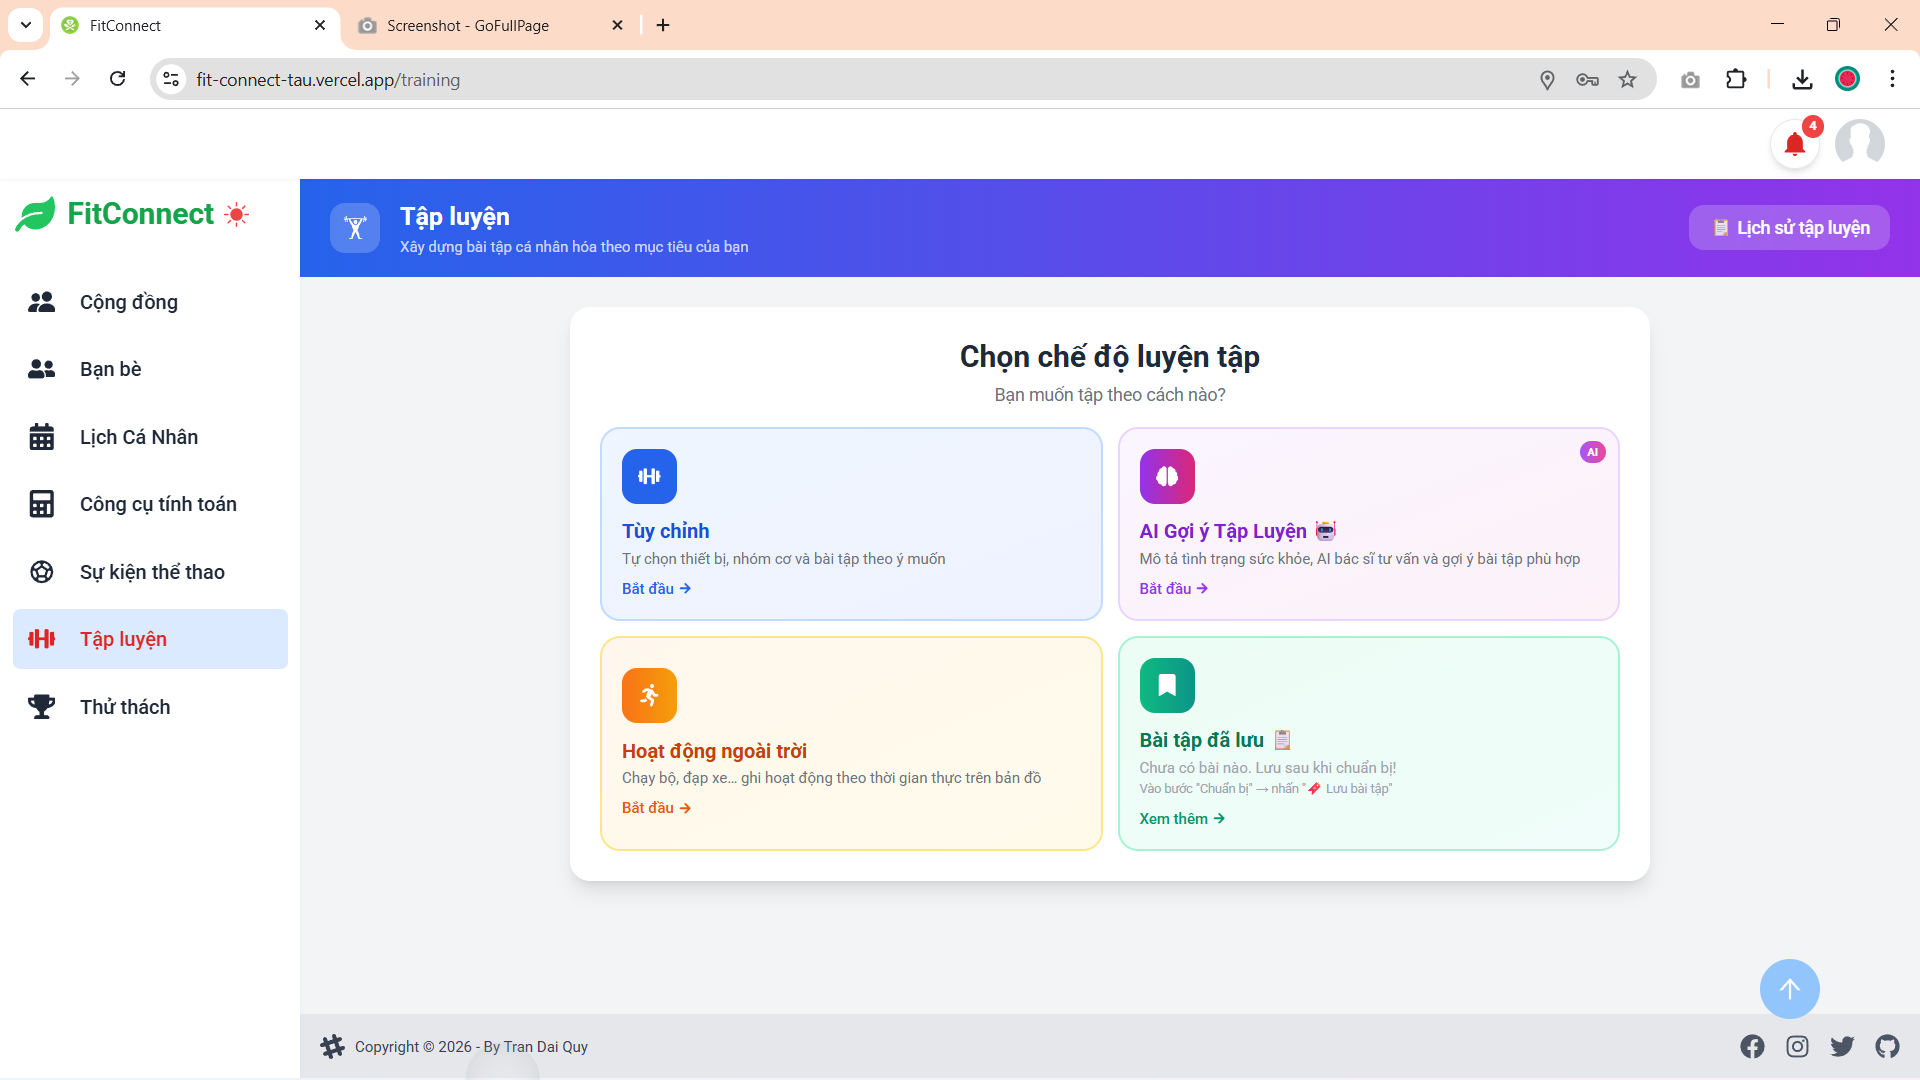
\includegraphics[width=0.60\textwidth]{Images/IMG/nhom5/manhinhtapluyen.png}
    \caption{Hệ thống hiển thị trang Tập luyện với 4 chế độ luyện tập}
    \label{fig:impl_train_main}
\end{figure}


    \item Khi chọn chế độ ``Tùy chỉnh'', hệ thống bắt đầu quy trình 5 bước. \textbf{Bước 1 -- Thiết bị}: Hệ thống hiển thị giao diện ``Chọn thiết bị của bạn'' với 8 loại thiết bị tập: Cơ thể (không cần thiết bị), Dây kháng lực (Resistance Band / Cable), Ghế tập (Bench), Máy / Đĩa tạ (Machine / Plate), Tạ tay (Dumbbell), Tạ đòn (Barbell), Tạ ấm (Kettlebell), và Xà đơn (Pull-up bar). Người dùng chọn các thiết bị có sẵn và nhấn ``Tiếp tục''.

\begin{figure}[H]
    \centering
    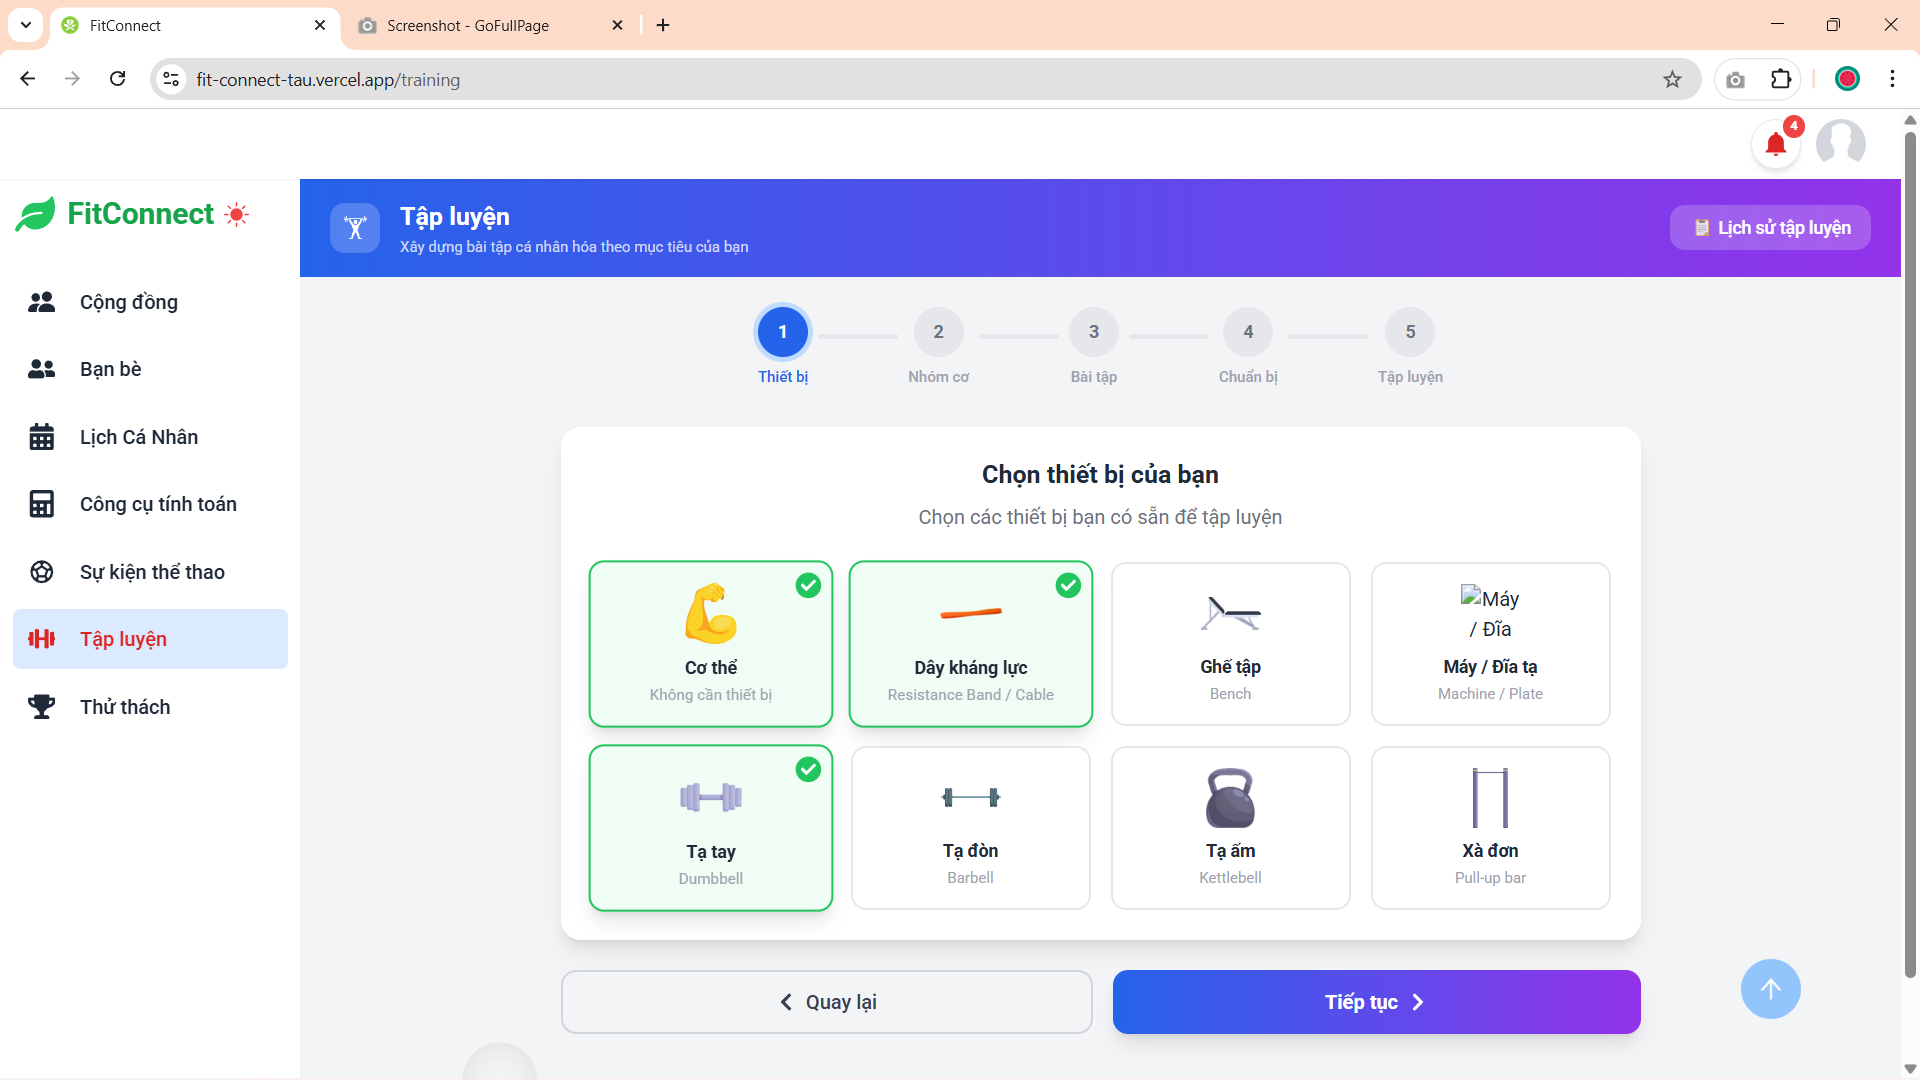
\includegraphics[width=0.60\textwidth]{Images/IMG/nhom5/chonthietbitap.png}
    \caption{Người dùng chọn thiết bị tập luyện có sẵn tại Bước 1}
    \label{fig:impl_train_equipment}
\end{figure}


    \item \textbf{Bước 2 -- Nhóm cơ}: Hệ thống hiển thị mô hình cơ thể người tương tác (mặt trước và mặt sau). Người dùng nhấn trực tiếp vào các vùng cơ trên mô hình để chọn nhóm cơ muốn tập (ví dụ: Vai trước, Bắp tay trước, Cẳng tay, Chéo bụng, Bụng, Ngực, Đùi trước,...). Các vùng cơ được chọn sẽ sáng lên màu xanh trên mô hình và hiển thị dưới dạng tag ở phía trên. Nhấn ``Tiếp tục'' để chuyển bước.

\begin{figure}[H]
    \centering
    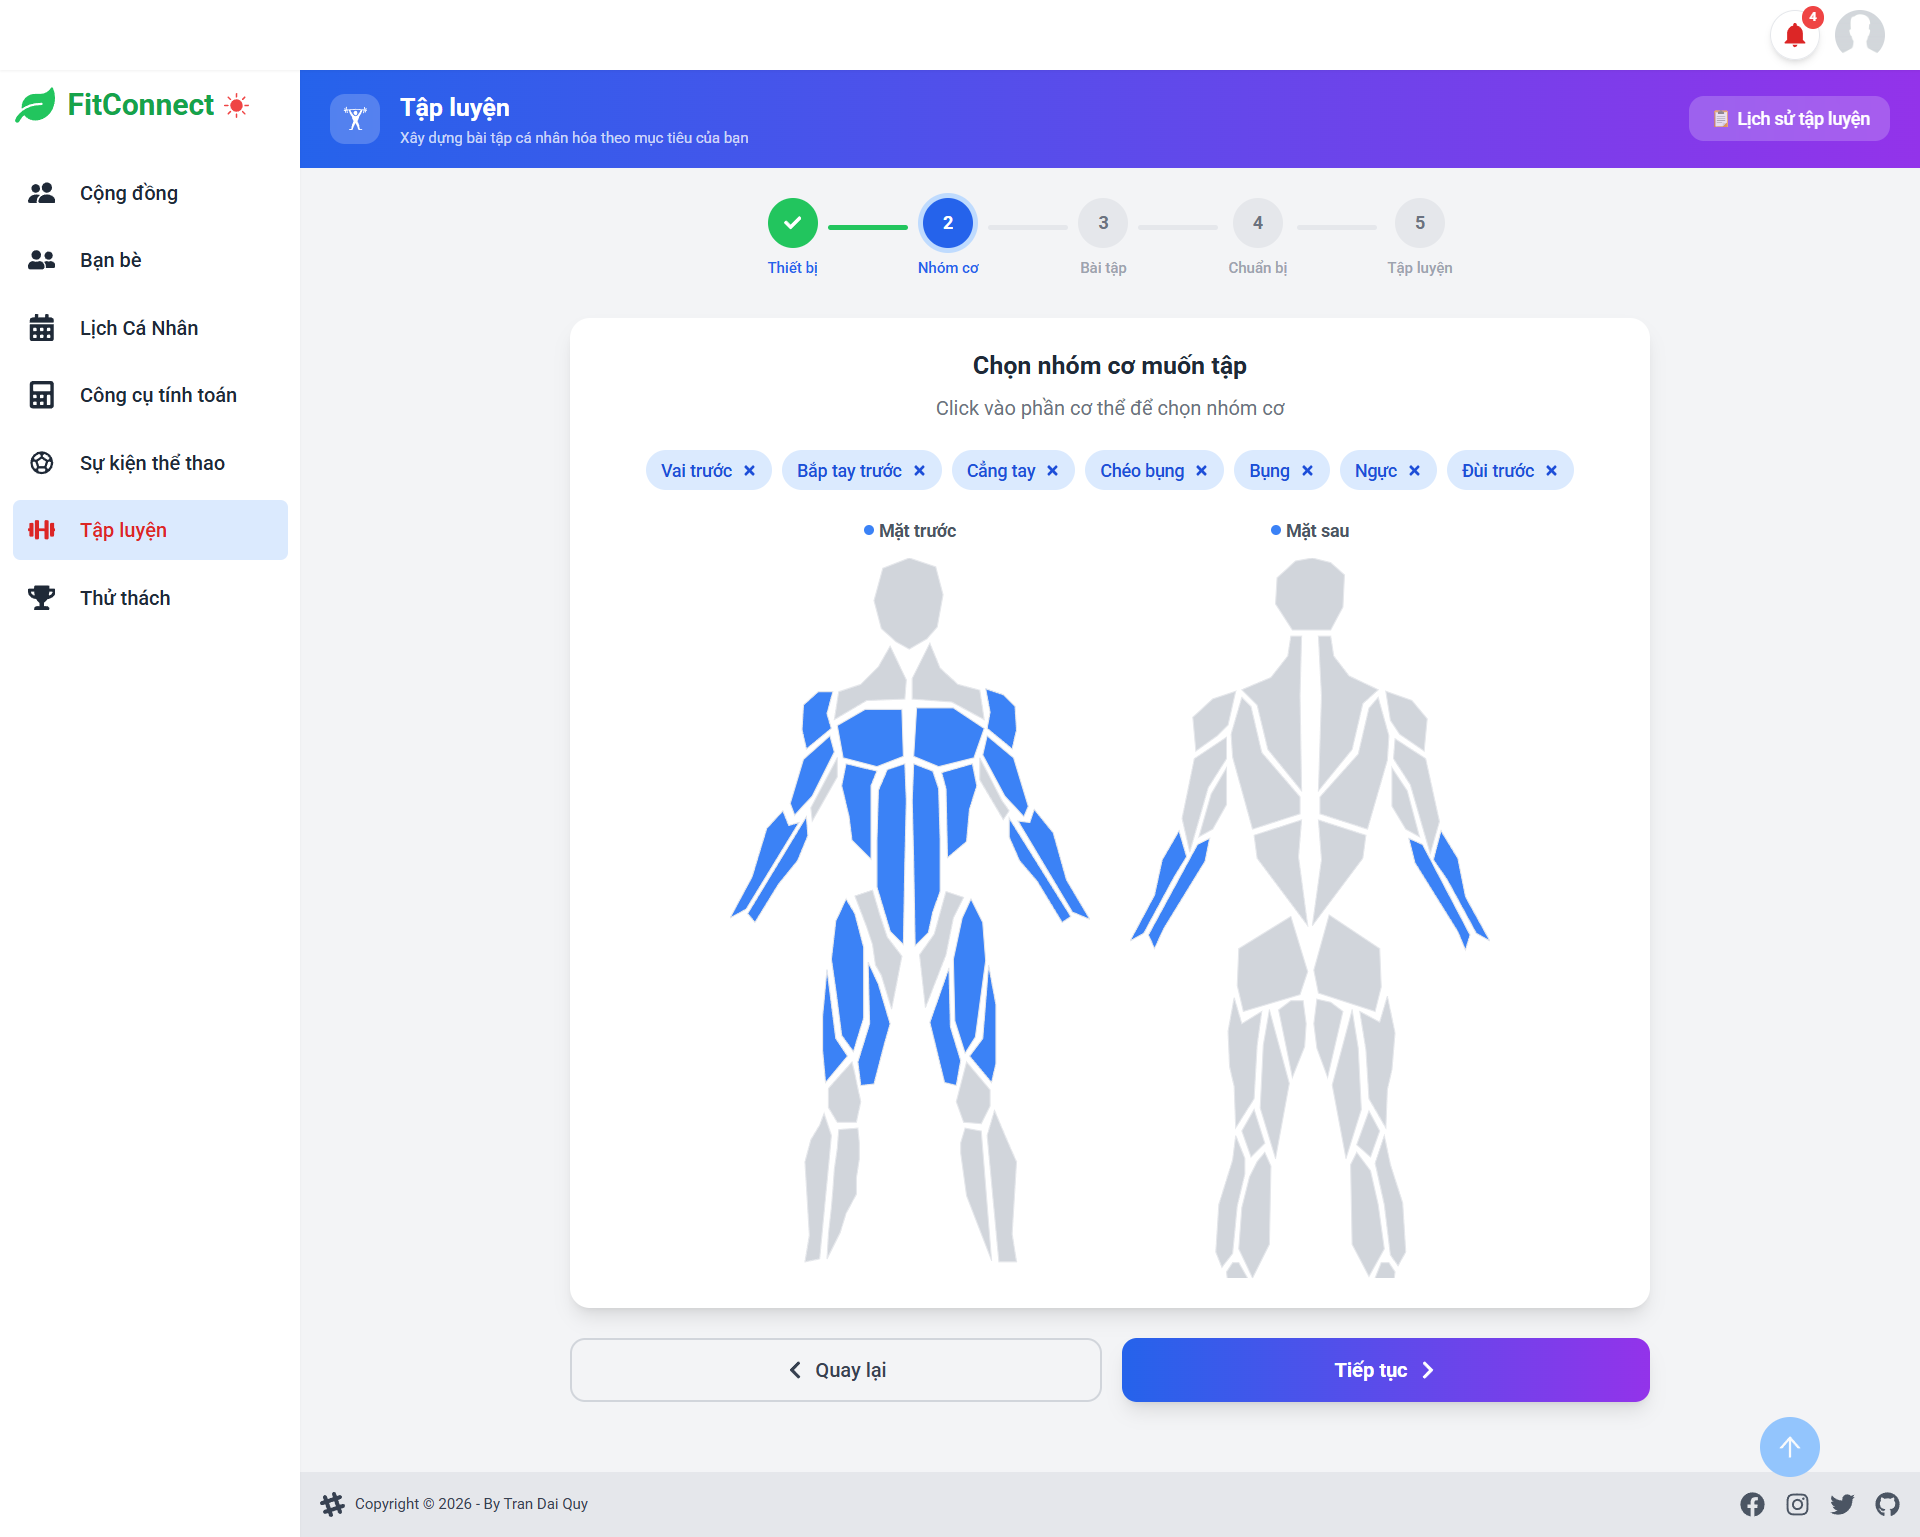
\includegraphics[width=0.60\textwidth]{Images/IMG/nhom5/chonnhomco.png}
    \caption{Người dùng chọn nhóm cơ muốn tập trên mô hình cơ thể tương tác tại Bước 2}
    \label{fig:impl_train_muscle}
\end{figure}


    \item \textbf{Bước 3 -- Bài tập}: Hệ thống lọc và hiển thị danh sách bài tập phù hợp với thiết bị và nhóm cơ đã chọn. Mỗi bài tập hiển thị: tên tiếng Anh, tên tiếng Việt, mức độ (Dễ, Trung bình), số set và reps mặc định. Phần ``Đã chọn'' ở trên cho phép kéo thả để sắp xếp lại thứ tự. Người dùng nhấn vào biểu tượng thông tin để xem chi tiết bài tập.

\begin{figure}[H]
    \centering
    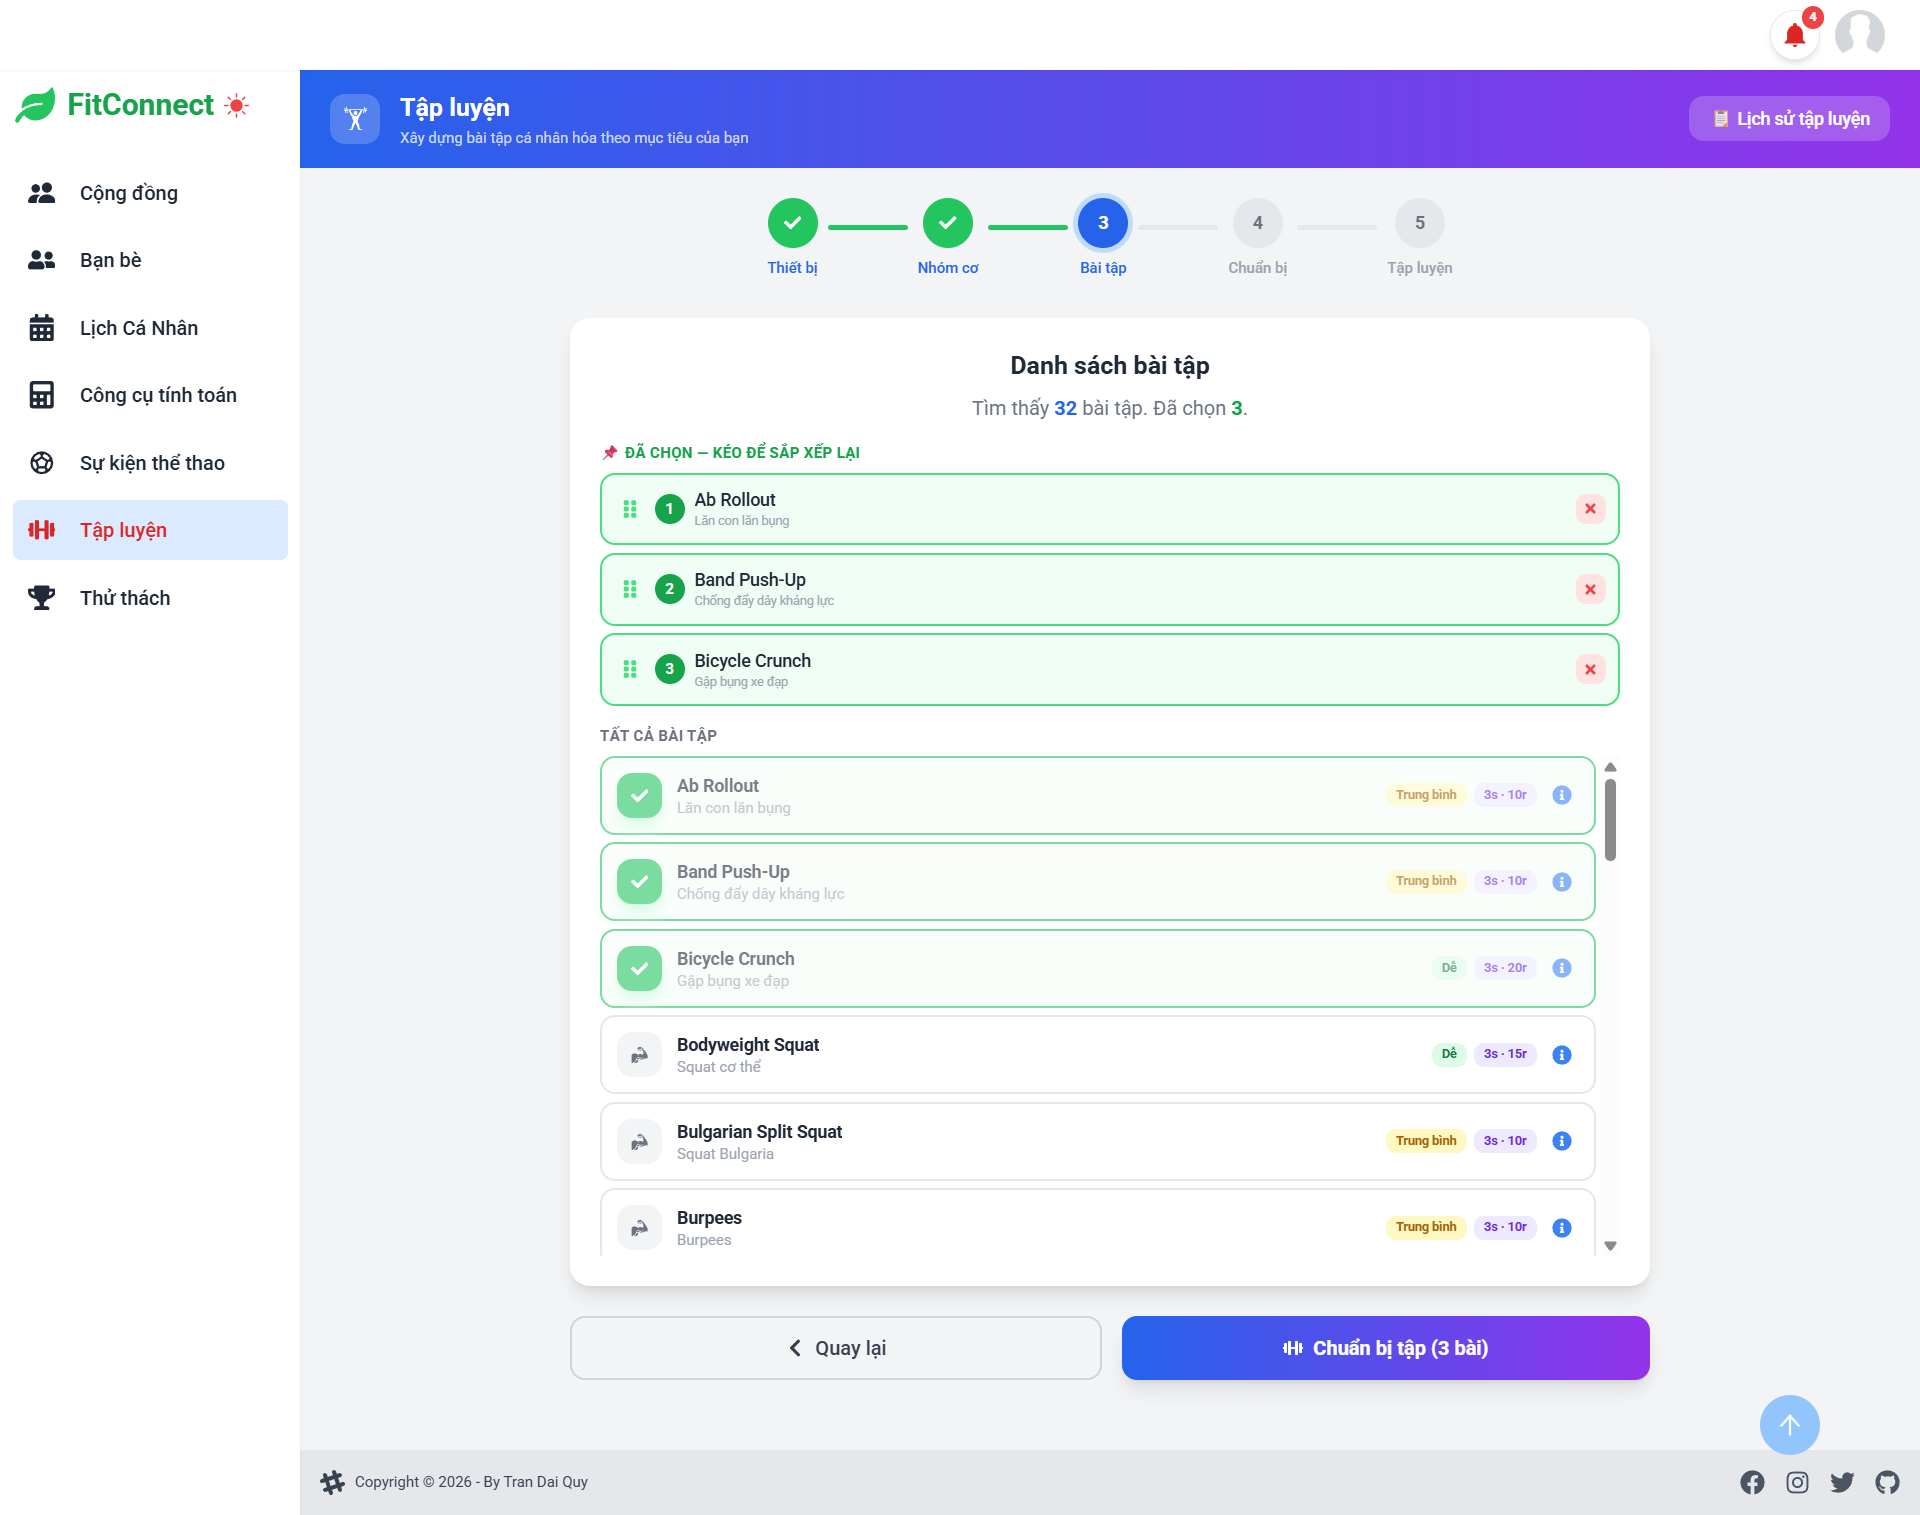
\includegraphics[width=0.60\textwidth]{Images/IMG/nhom5/chonbaitap.png}
    \caption{Người dùng chọn bài tập từ danh sách được lọc theo thiết bị và nhóm cơ tại Bước 3}
    \label{fig:impl_train_exercises}
\end{figure}


    \item Khi nhấn biểu tượng thông tin của một bài tập, hệ thống hiển thị modal chi tiết gồm: video hướng dẫn từ YouTube, tên bài tập (tiếng Anh và tiếng Việt), nhãn mức độ (Dễ), loại bài tập (Sức mạnh), lượng kcal/đơn vị, phần ``Hướng dẫn thực hiện'' với các bước chi tiết đánh số, và phần ``Mẹo'' với lời khuyên kỹ thuật.

\begin{figure}[H]
    \centering
    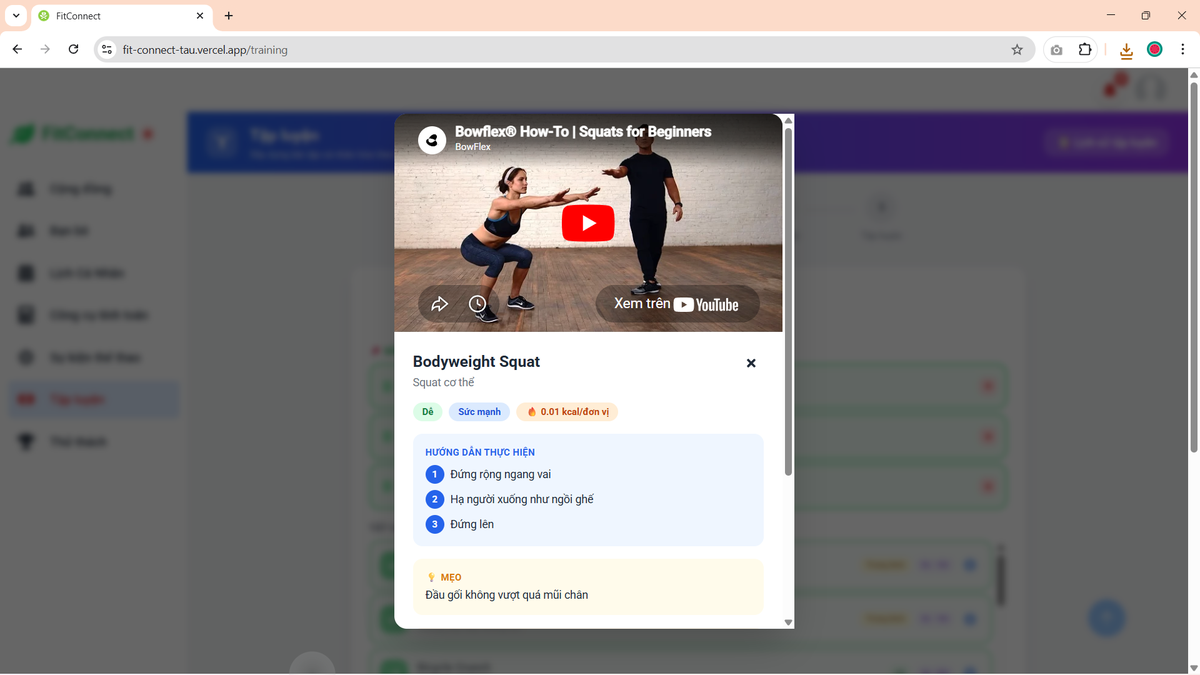
\includegraphics[width=0.60\textwidth]{Images/IMG/nhom5/xemthongtinbaitap.png}
    \caption{Hệ thống hiển thị thông tin chi tiết bài tập kèm video hướng dẫn}
    \label{fig:impl_train_detail}
\end{figure}


    \item \textbf{Bước 4 -- Chuẩn bị}: Sau khi chọn bài tập và nhấn ``Chuẩn bị tập'', hệ thống hiển thị trang Chuẩn bị tập luyện với tổng quan (số bài tập, tổng sets). Mỗi bài tập hiển thị bảng chi tiết gồm: SET, Reps (Số lần), Weight (Mức tạ -- kg), và kcal tự động tính. Người dùng có thể chỉnh sửa số lần, mức tạ, thêm set (nút ``+ Thêm set''), hoặc xóa set. Hệ thống hiển thị tổng kcal ước tính. Tại đây, người dùng có 3 lựa chọn: ``Quay lại'', ``Lưu bài tập'' (lưu giáo án cho lần sau), hoặc ``Bắt đầu tập!'' để bắt đầu tập luyện.

\begin{figure}[H]
    \centering
    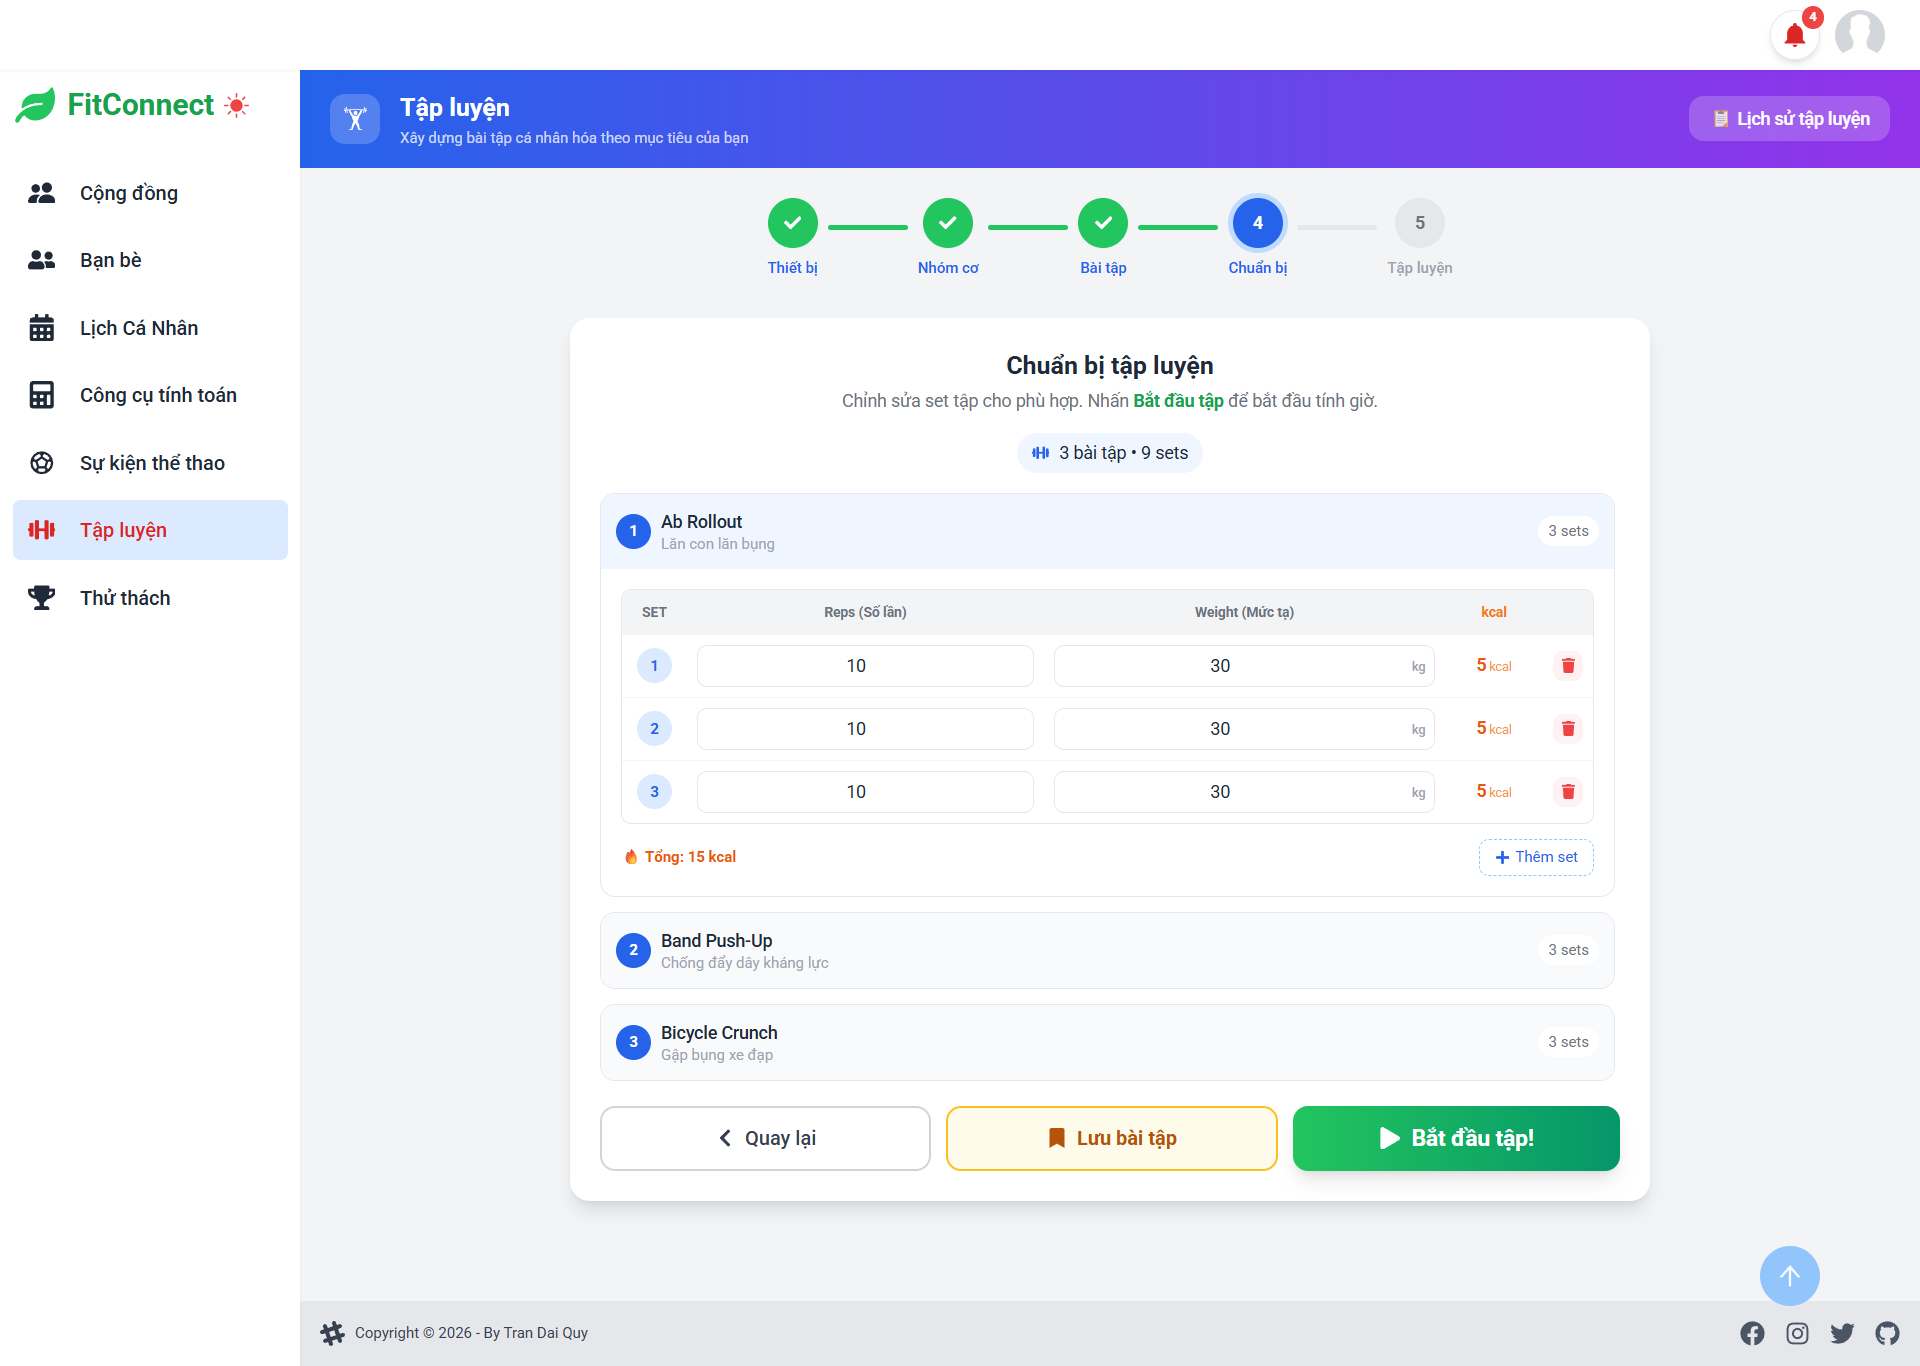
\includegraphics[width=0.60\textwidth]{Images/IMG/nhom5/buocchuanbitapluyen.png}
    \caption{Người dùng cấu hình sets, reps, mức tạ cho từng bài tập tại Bước 4 -- Chuẩn bị}
    \label{fig:impl_train_prep}
\end{figure}


    \item \textbf{Bước 5 -- Tập luyện}: Khi nhấn ``Bắt đầu tập!'', hệ thống chuyển sang trang Tập luyện hiển thị 3 thông số theo dõi thời gian thực: Thời gian (đồng hồ đếm), Bài tập (số bài hoàn thành/tổng, phần trăm), và kcal đã đốt. Mỗi bài tập hiển thị từng set với thông tin (số lần, mức tạ, kcal). Người dùng nhấn ``Xong'' cho từng set sau khi hoàn thành, sau đó nhấn ``Bài tiếp'' để chuyển sang bài tập kế tiếp. Phần ``Tất cả bài tập'' ở dưới hiển thị tiến độ tổng thể với đánh dấu xanh cho các bài đã hoàn thành. Người dùng cũng có thể nhấn ``Bỏ tập'' nếu muốn hủy buổi tập.

\begin{figure}[H]
    \centering
    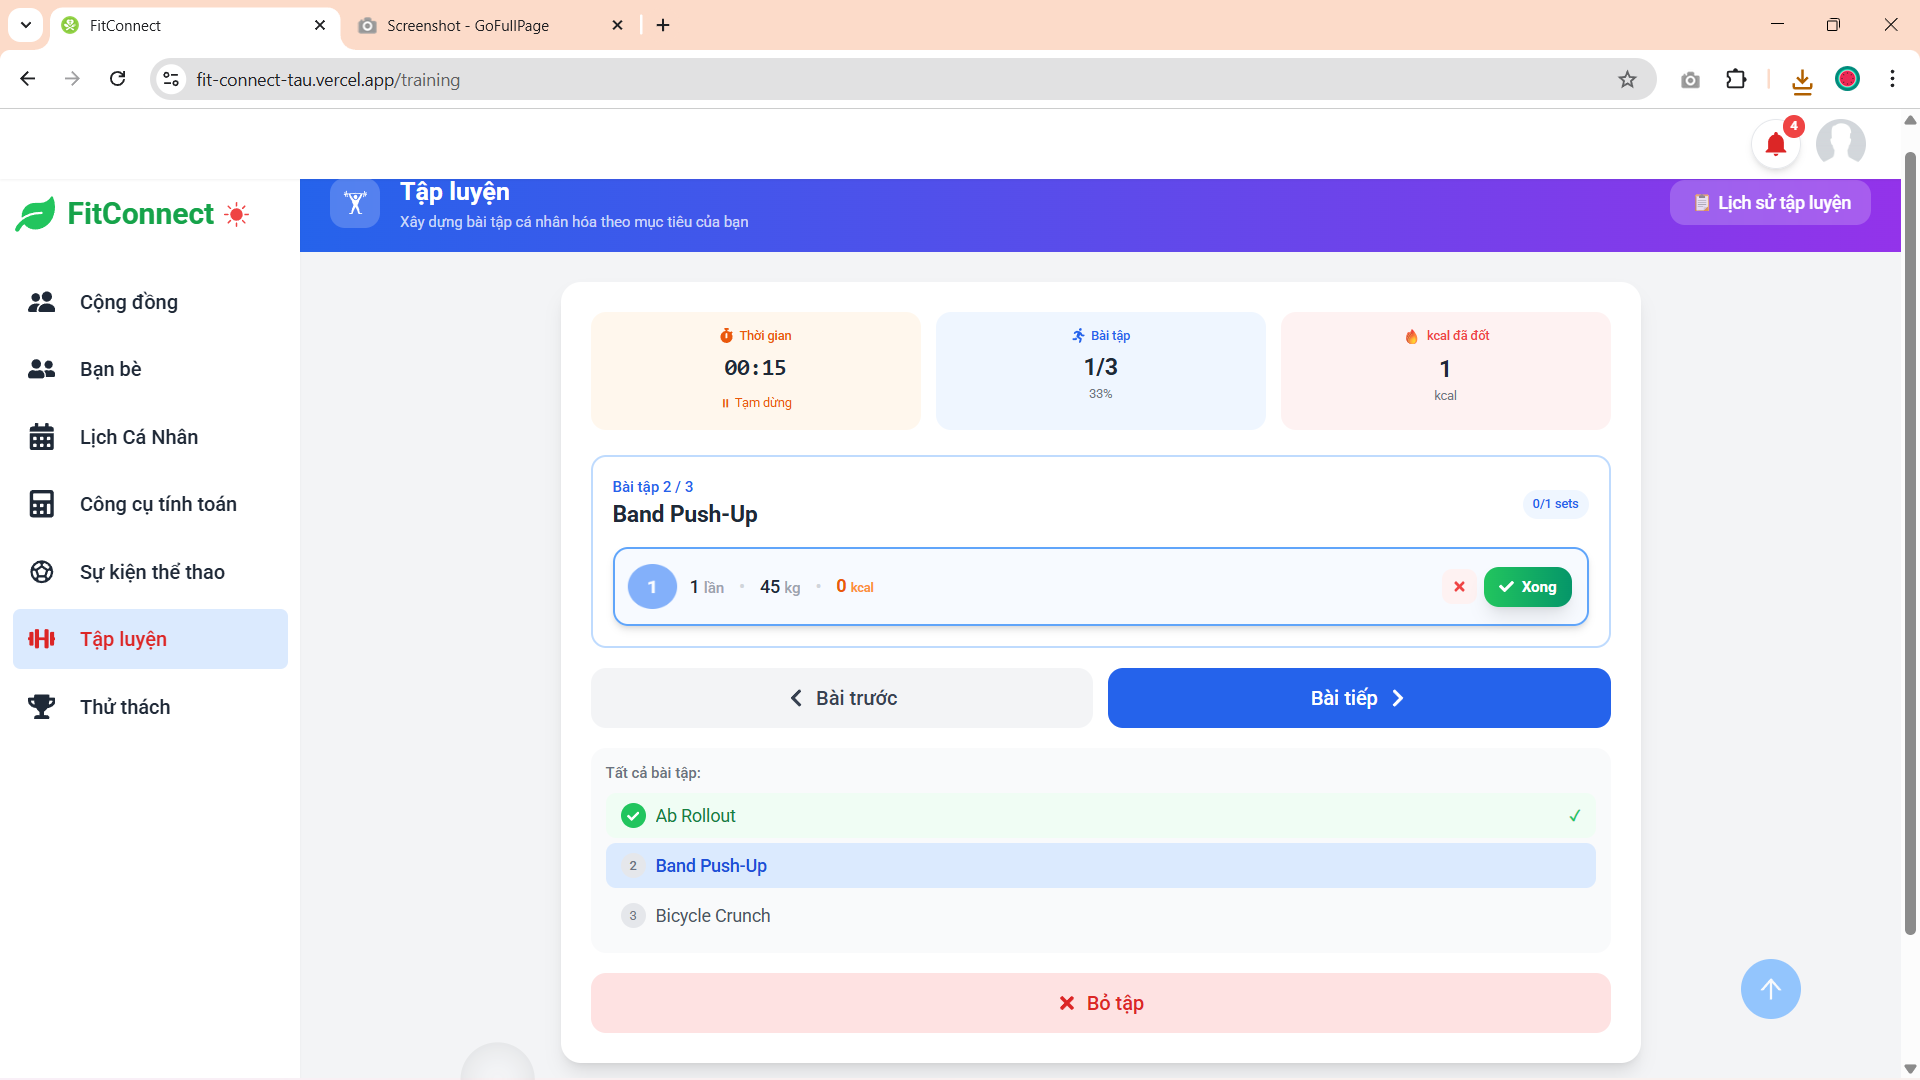
\includegraphics[width=0.60\textwidth]{Images/IMG/nhom5/tabbatdautapluyen.png}
    \caption{Người dùng thực hiện tập luyện và theo dõi tiến độ từng set tại Bước 5}
    \label{fig:impl_train_active}
\end{figure}


    \item Sau khi hoàn thành tất cả bài tập, hệ thống hiển thị trạng thái 100\% và nút ``Hoàn thành tập luyện''. Khi xác nhận, buổi tập được ghi nhận tự động vào lịch sử tập luyện.

\end{itemize}

\subsubsection{Luồng tập luyện AI Gợi ý}

\begin{itemize}
    \item Khi chọn chế độ ``AI Gợi ý Tập Luyện'', hệ thống hiển thị giao diện với ô nhập liệu ``Mô tả tình trạng và mục tiêu tập luyện''. Người dùng nhập mô tả tình trạng sức khỏe hiện tại bằng ngôn ngữ tự nhiên (ví dụ: ``Tôi bị đau lưng, cho tôi các bài viết nhẹ nhàng'') và nhấn nút ``Phân tích AI''.

\begin{figure}[H]
    \centering
    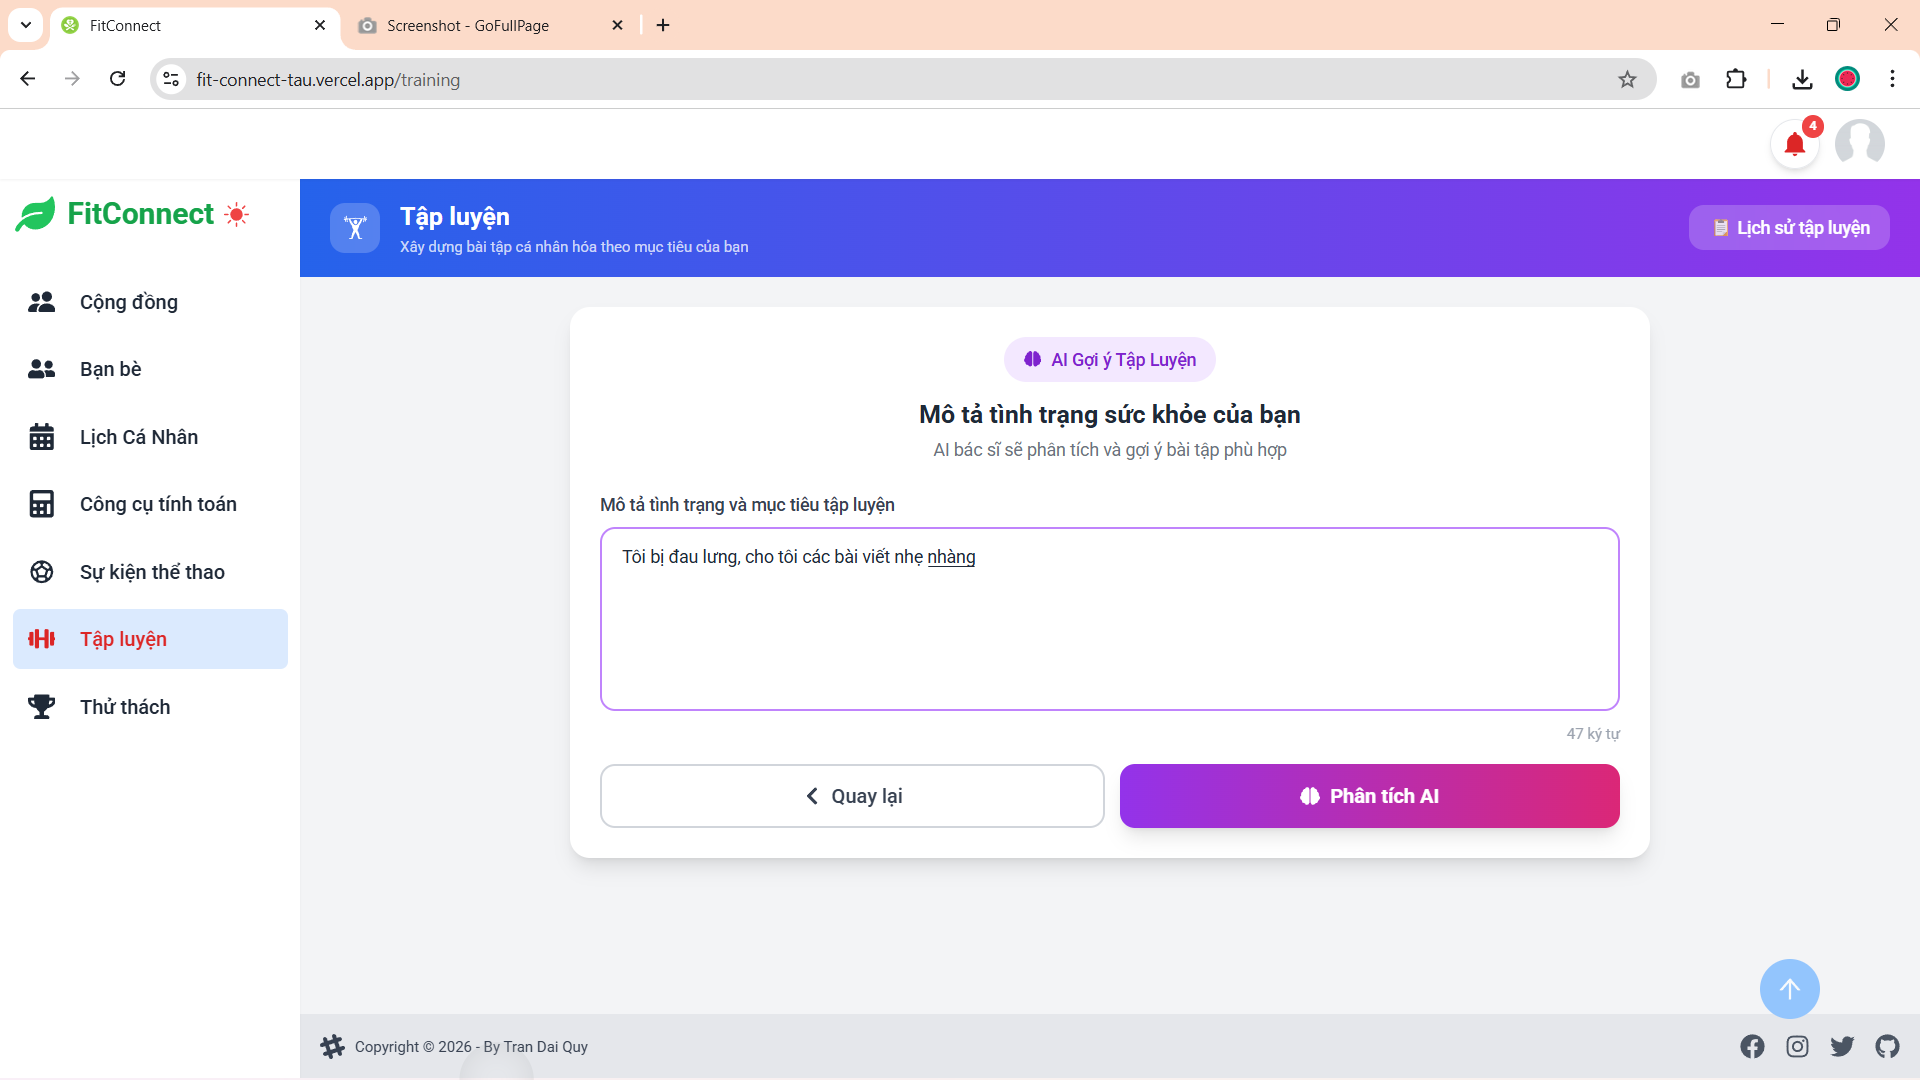
\includegraphics[width=0.60\textwidth]{Images/IMG/nhom5/manhinhAIgoiybaitap.png}
    \caption{Người dùng nhập mô tả tình trạng sức khỏe để AI phân tích và gợi ý bài tập}
    \label{fig:impl_train_ai_input}
\end{figure}


    \item Hệ thống gửi mô tả tới AI, AI phân tích và trả về kết quả gồm: phần ``Đánh giá sức khỏe từ bác sĩ'' với nhận xét chi tiết về tình trạng sức khỏe và khuyến nghị, và phần ``Bài tập gợi ý'' với danh sách bài tập phù hợp. Mỗi bài tập hiển thị: tên, nhãn mức độ (Dễ, Trung bình), loại bài tập (Sức mạnh), và lý do AI gợi ý. Người dùng chọn các bài tập muốn tập (phần ``Đã chọn'' hiển thị số lượng) và nhấn ``Bắt đầu luyện tập'' để chuyển sang trang Chuẩn bị.

\begin{figure}[H]
    \centering
    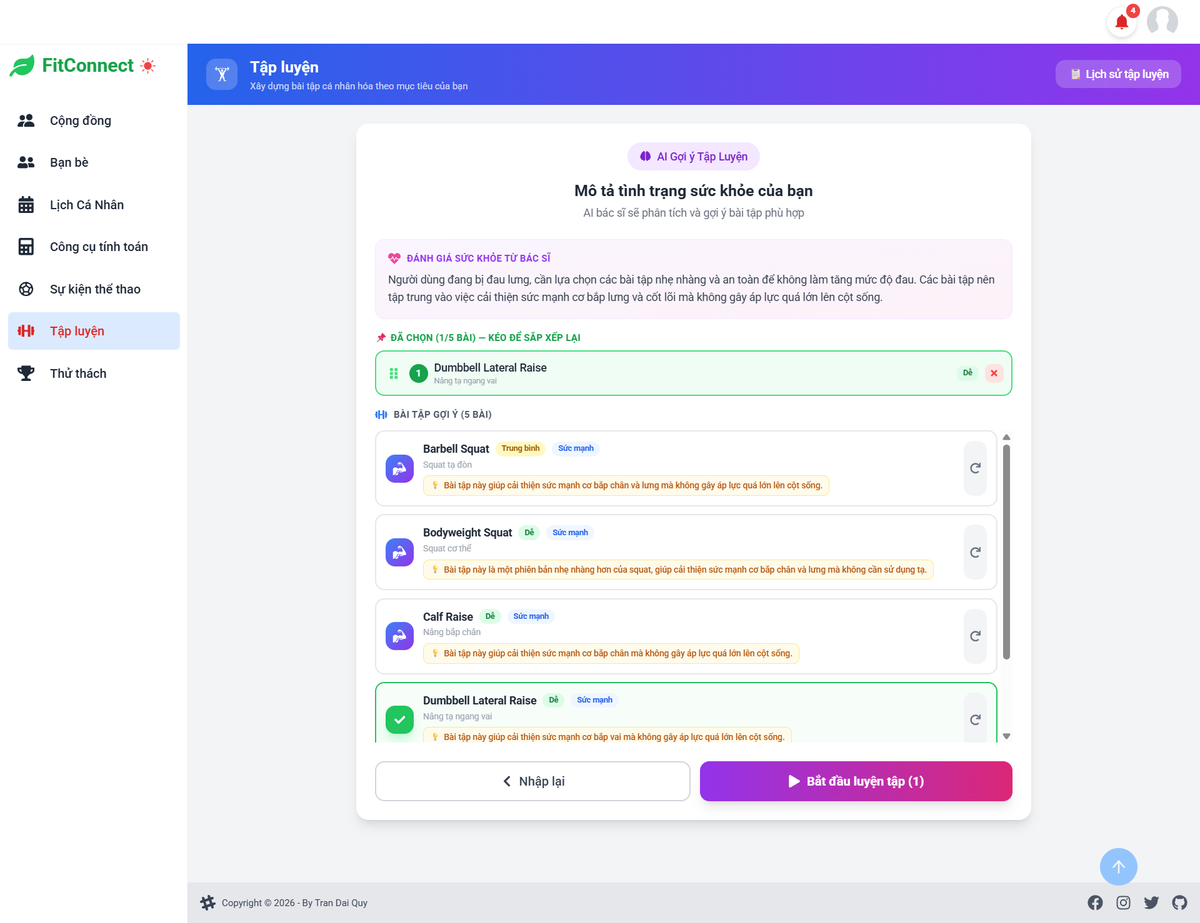
\includegraphics[width=0.60\textwidth]{Images/IMG/nhom5/aigoigoiydanhsachbaitap.png}
    \caption{Hệ thống AI phân tích sức khỏe và gợi ý danh sách bài tập phù hợp}
    \label{fig:impl_train_ai_result}
\end{figure}


    \item Sau khi chọn bài tập từ AI, hệ thống chuyển sang trang Chuẩn bị tập luyện tương tự luồng Tùy chỉnh (nhưng chỉ gồm 2 bước: Chuẩn bị và Tập luyện). Người dùng có thể chỉnh sửa sets, reps, mức tạ và bắt đầu tập luyện.

\begin{figure}[H]
    \centering
    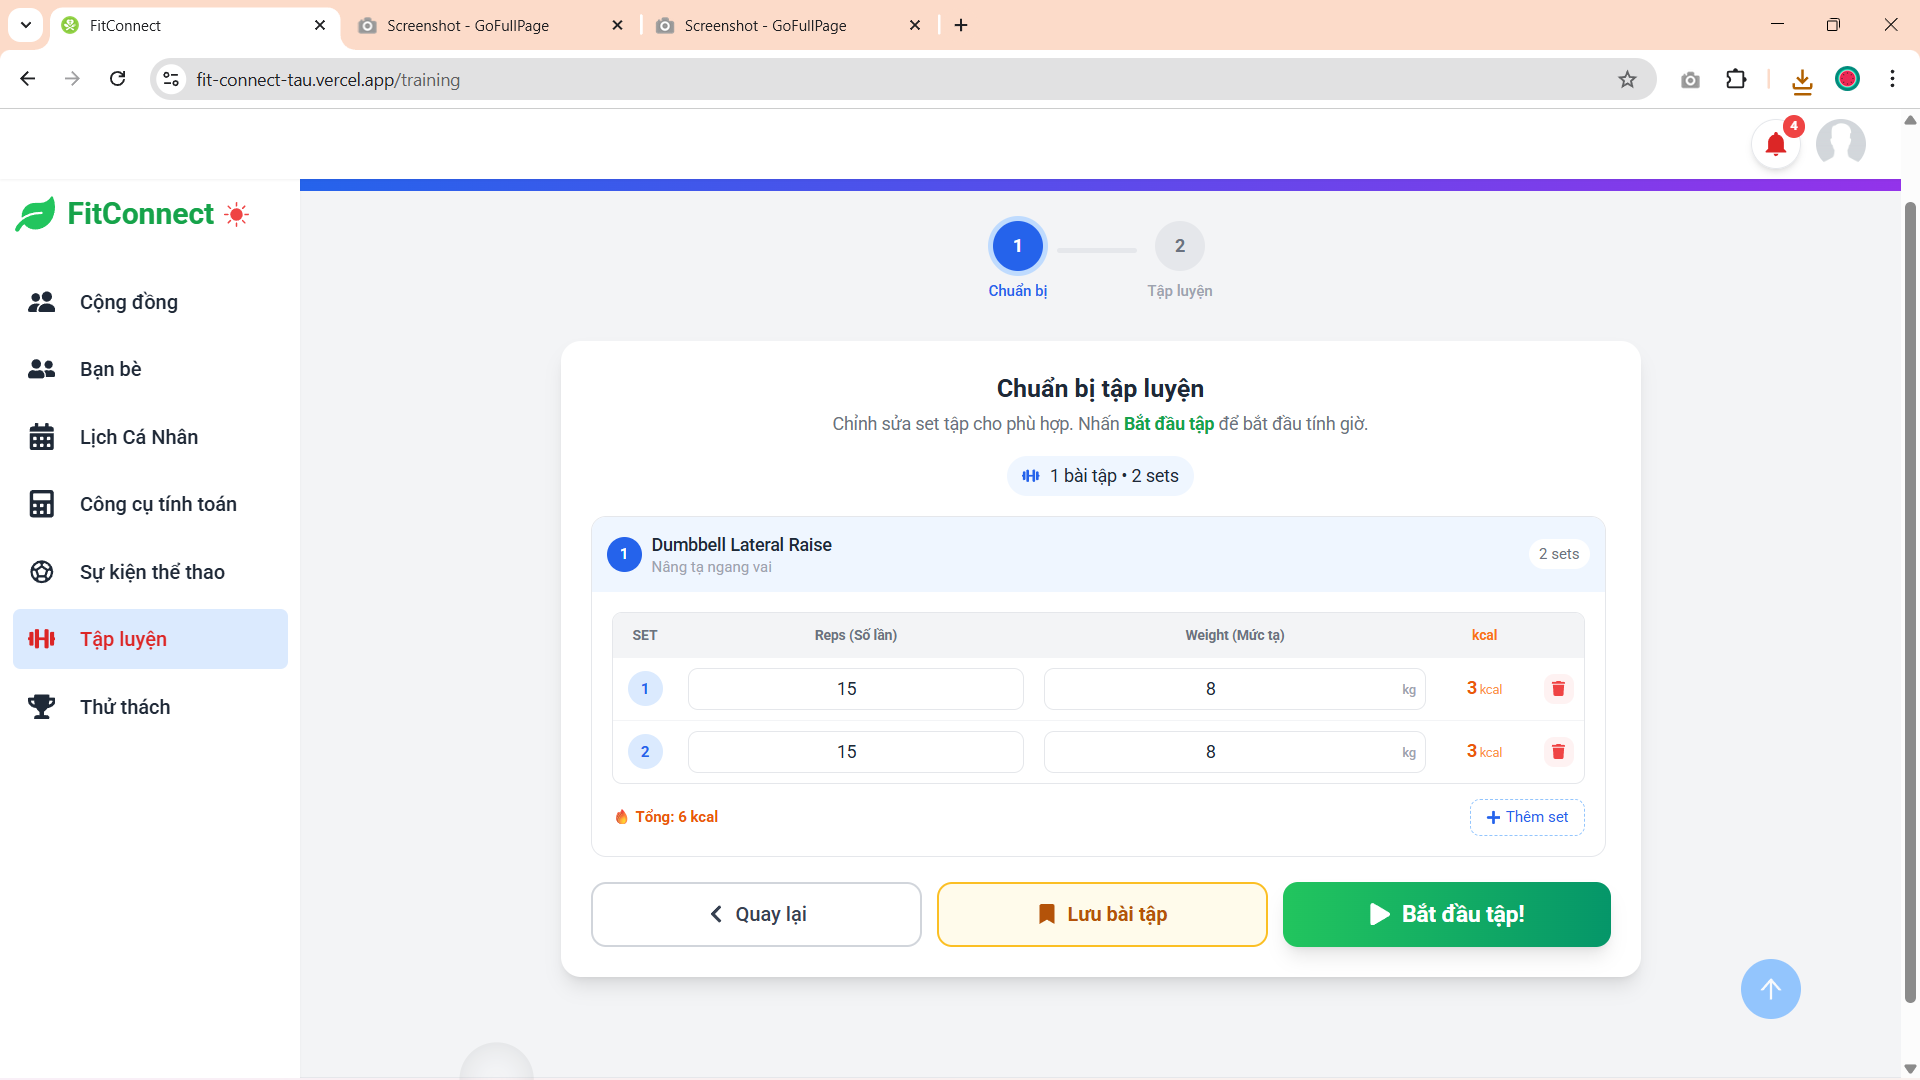
\includegraphics[width=0.60\textwidth]{Images/IMG/nhom5/manhinhchuanbitapluyentuAIqua.png}
    \caption{Người dùng chuẩn bị tập luyện với bài tập được AI gợi ý}
    \label{fig:impl_train_ai_prep}
\end{figure}

\end{itemize}

\subsubsection{Luồng Hoạt động ngoài trời}

\begin{itemize}
    \item Khi chọn chế độ ``Hoạt động ngoài trời'', hệ thống hiển thị trang thiết lập hoạt động gồm: lựa chọn môn thể thao (Chạy bộ đường dài, Đạp xe,...) kèm kcal/km ước tính, ô nhập tên bài tập, và quãng đường mục tiêu (km). Phần Tóm tắt hiển thị thông tin đã chọn. Người dùng nhấn ``Bắt đầu ghi'' để khởi động theo dõi GPS.

\begin{figure}[H]
    \centering
    
\includegraphics[width=0.60\textwidth]{Images/IMG/nhom5/tapluyenchaybo.png}
    \caption{Người dùng thiết lập hoạt động ngoài trời trước khi bắt đầu ghi GPS}
    \label{fig:impl_train_outdoor_setup}
\end{figure}


    \item Hệ thống mở giao diện GPS Tracking toàn màn hình hiển thị bản đồ thời gian thực với vị trí hiện tại. Phía dưới bản đồ, hệ thống hiển thị các thông số theo dõi: quãng đường (KM), thời gian (THỜI GIAN), tốc độ (KM/H), kcal đã đốt (KCAL), và thanh tiến trình quãng đường mục tiêu. Nút tạm dừng/tiếp tục cho phép người dùng kiểm soát buổi tập.

\begin{figure}[H]
    \centering
    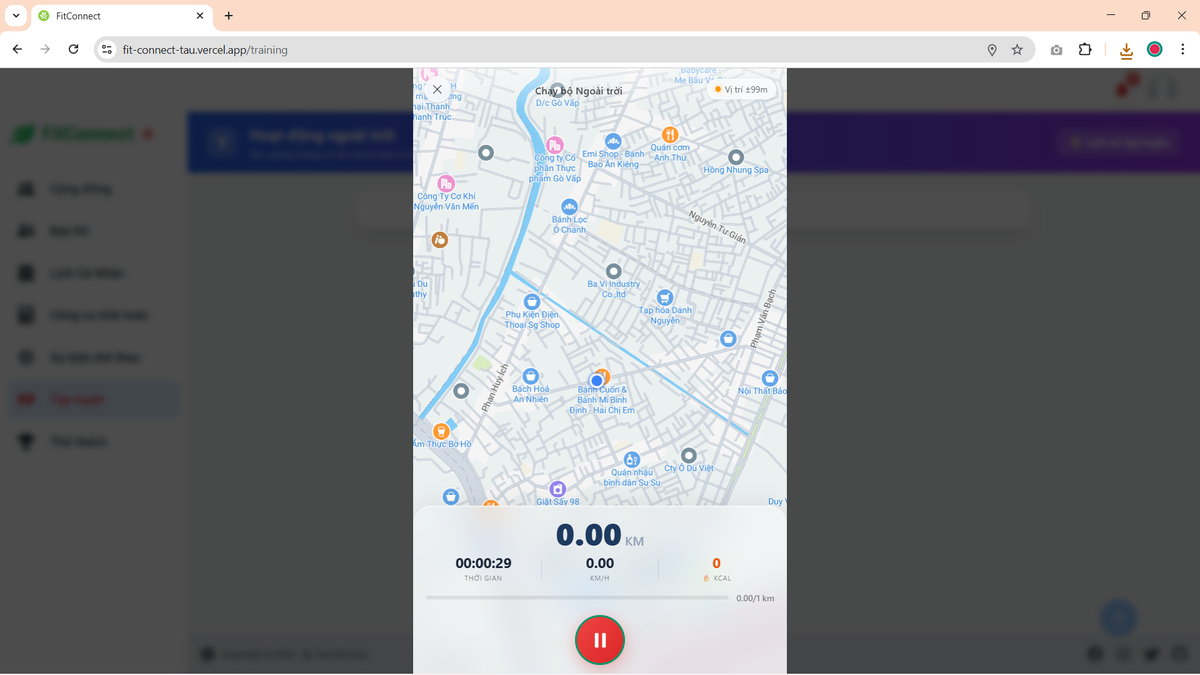
\includegraphics[width=0.60\textwidth]{Images/IMG/nhom5/manhinhtrackinggpstapluyen.png}
    \caption{Hệ thống theo dõi GPS thời gian thực trên bản đồ khi chạy bộ ngoài trời}
    \label{fig:impl_train_gps}
\end{figure}


    \item Khi dừng hoạt động, hệ thống tổng kết kết quả: quãng đường (km), thời gian, và kcal đã đốt. Người dùng nhấn ``Xác nhận'' để lưu vào lịch sử hoặc ``Quay lại'' để tiếp tục hoạt động.

\end{itemize}

\subsubsection{Lưu giáo án và đặt lịch tập}

\begin{itemize}
    \item Tại bước Chuẩn bị tập luyện, khi nhấn ``Lưu bài tập'', hệ thống hiển thị modal ``Lưu bài tập'' yêu cầu nhập tên bài tập (ví dụ: ``Tập lưng'') và hiển thị thông tin tóm tắt (số bài, số sets sẽ được lưu). Người dùng nhấn ``Tiếp tục'' để lưu.

\begin{figure}[H]
    \centering
    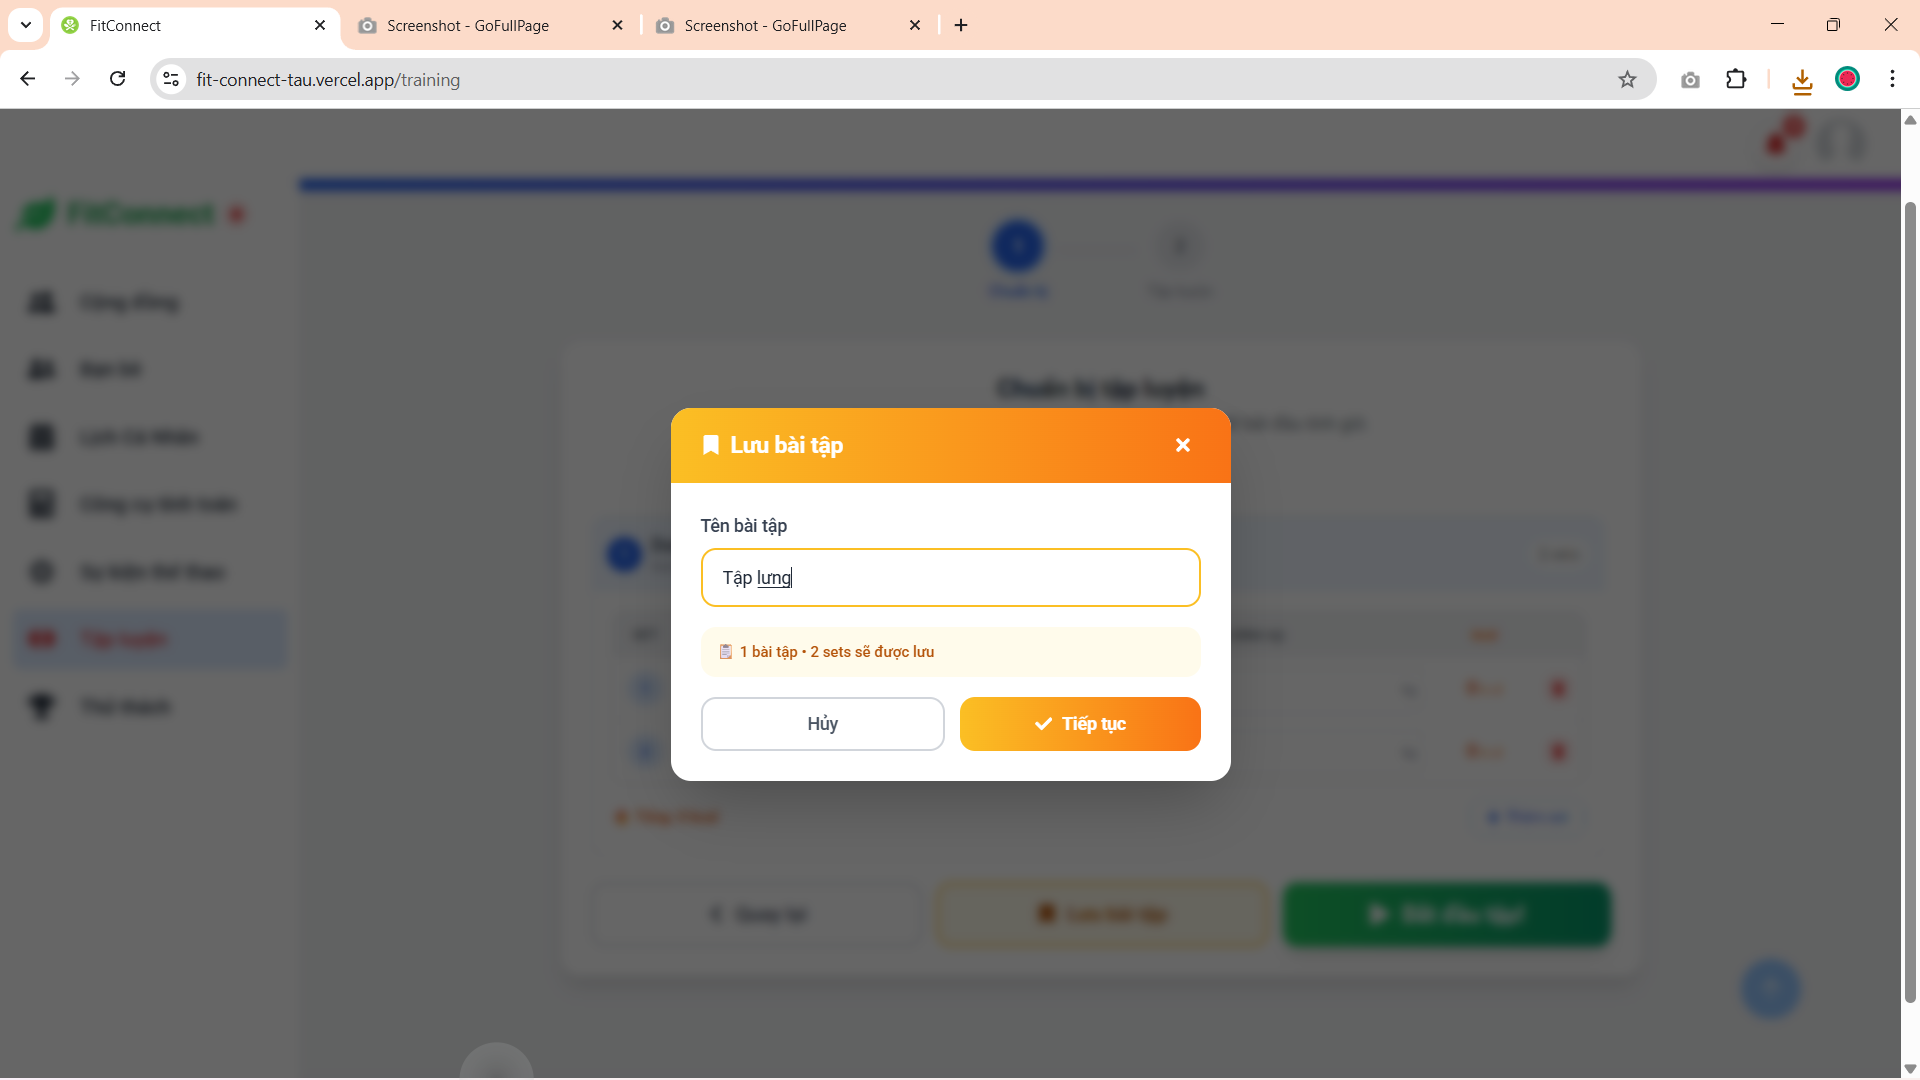
\includegraphics[width=0.60\textwidth]{Images/IMG/nhom5/modalluulichtap.png}
    \caption{Người dùng nhập tên và lưu giáo án tập luyện}
    \label{fig:impl_train_save}
\end{figure}


    \item Sau khi lưu, hệ thống hiển thị modal ``Đặt lịch tập?'' hỏi người dùng có muốn đặt lịch tập định kỳ không. Nếu chọn ``Đặt lịch!'', hệ thống hiển thị modal ``Cài đặt lịch tập'' cho phép chọn: Ngày tập trong tuần (CN, T2, T3,..., T7), Giờ tập, khoảng thời gian (Từ ngày -- Đến ngày), và tùy chọn ``Nhắc nhở khi mở app'' (hiển thị thông báo vào ngày tập theo lịch). Nhấn ``Lưu \& Đặt lịch'' để hoàn tất.

\begin{figure}[H]
    \centering
    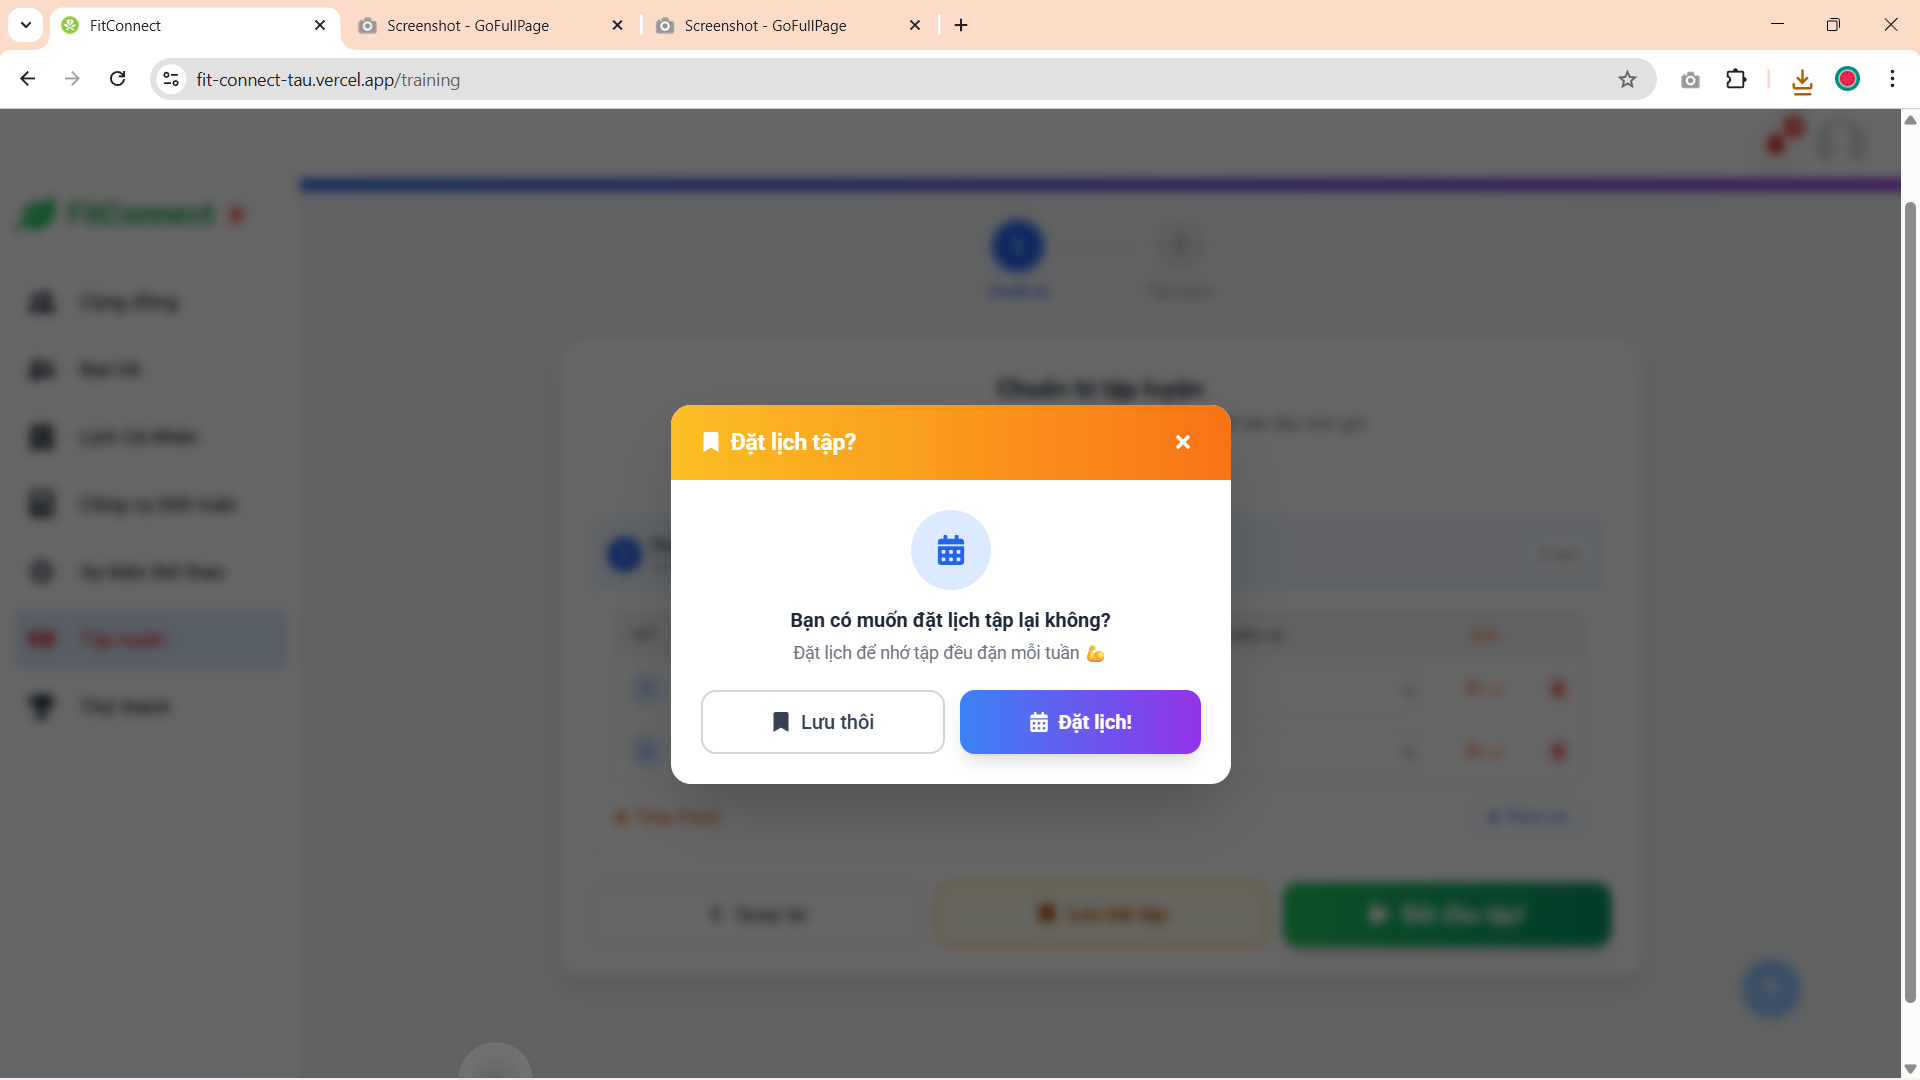
\includegraphics[width=0.60\textwidth]{Images/IMG/nhom5/modaldatlichtap.png}
    \caption{Người dùng cài đặt lịch tập định kỳ với ngày, giờ và nhắc nhở}
    \label{fig:impl_train_schedule}
\end{figure}


    \item Khi chọn chế độ ``Bài tập đã lưu'' từ trang chủ Tập luyện, hệ thống hiển thị modal ``Bài tập đã lưu'' với danh sách giáo án đã lưu, mỗi giáo án hiển thị: tên, số bài tập, số sets, ngày lưu, lịch tập đã đặt (ví dụ: T2, T3, T4 lúc 10:00), nút đặt lịch, nút xóa, và nút ``Tập ngay!''.

\begin{figure}[H]
    \centering
    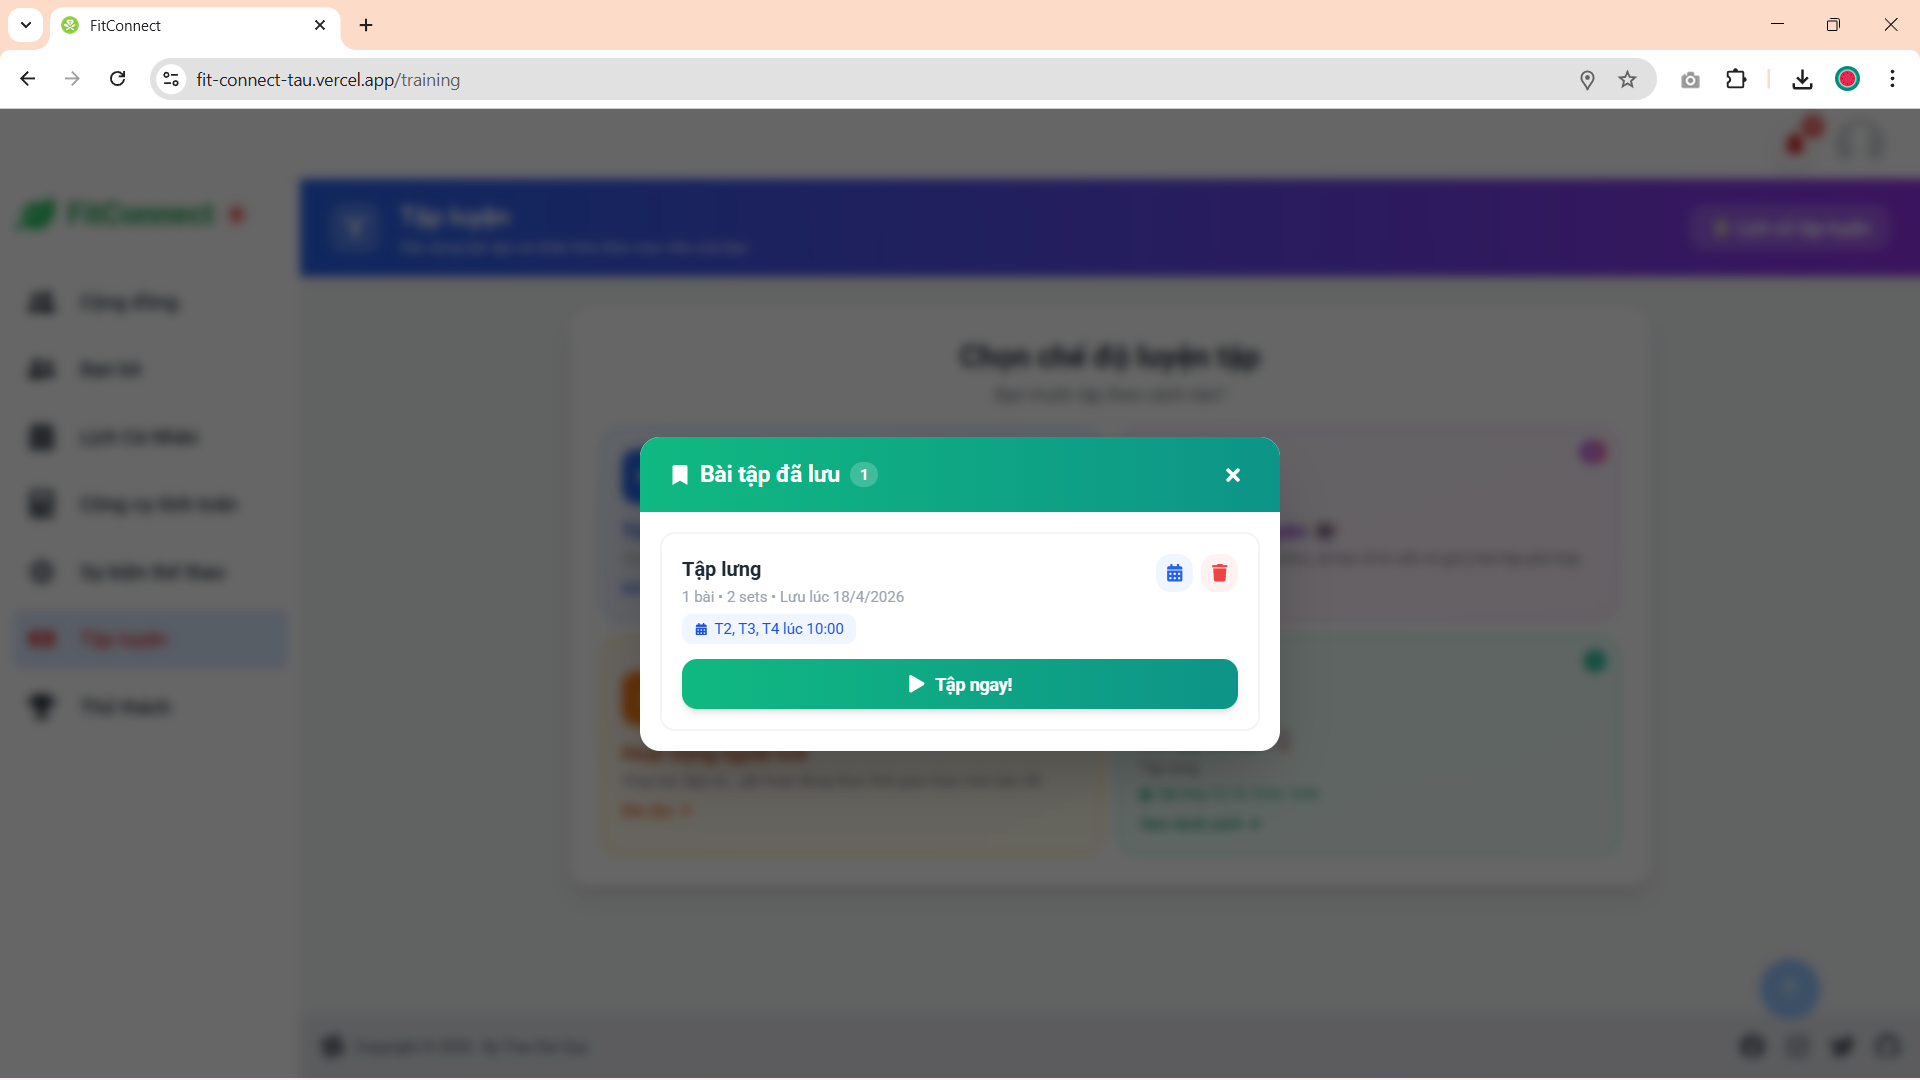
\includegraphics[width=0.60\textwidth]{Images/IMG/nhom5/danhsachbaitapdaluu.png}
    \caption{Hệ thống hiển thị danh sách giáo án tập luyện đã lưu}
    \label{fig:impl_train_saved_list}
\end{figure}

\end{itemize}

\subsubsection{Lịch sử tập luyện}

\begin{itemize}
    \item Người dùng nhấn ``Lịch sử tập luyện'' từ góc phải trang Tập luyện. Hệ thống chuyển sang trang Lịch sử tập luyện hiển thị 2 tab: ``Thời gian trong gym'' và ``Hoạt động ngoài trời''. Tại tab Thời gian trong gym, hệ thống hiển thị bộ lọc thời gian (7 ngày, 30 ngày,...), tổng số hoạt động và tổng thời gian tập. Mỗi buổi tập hiển thị: số bài tập, trạng thái (Hoàn thành), ngày giờ, tổng SETS, tổng KCAL, thời gian (PHÚT), chi tiết từng bài tập kèm số set, và danh sách nhóm cơ cùng thiết bị đã tập.

\begin{figure}[H]
    \centering
    
\includegraphics[width=0.60\textwidth]{Images/IMG/nhom5/lichsutapluyen.png}
    \caption{Hệ thống hiển thị lịch sử tập luyện trong gym với chi tiết từng buổi tập}
    \label{fig:impl_train_history_gym}
\end{figure}


    \item Tại tab ``Hoạt động ngoài trời'', hệ thống hiển thị danh sách các hoạt động ngoài trời đã thực hiện. Mỗi hoạt động hiển thị: tên bài tập, loại hoạt động, ngày giờ, quãng đường (km), tốc độ (km/h), kcal đã đốt, và thời gian.

\begin{figure}[H]
    \centering
    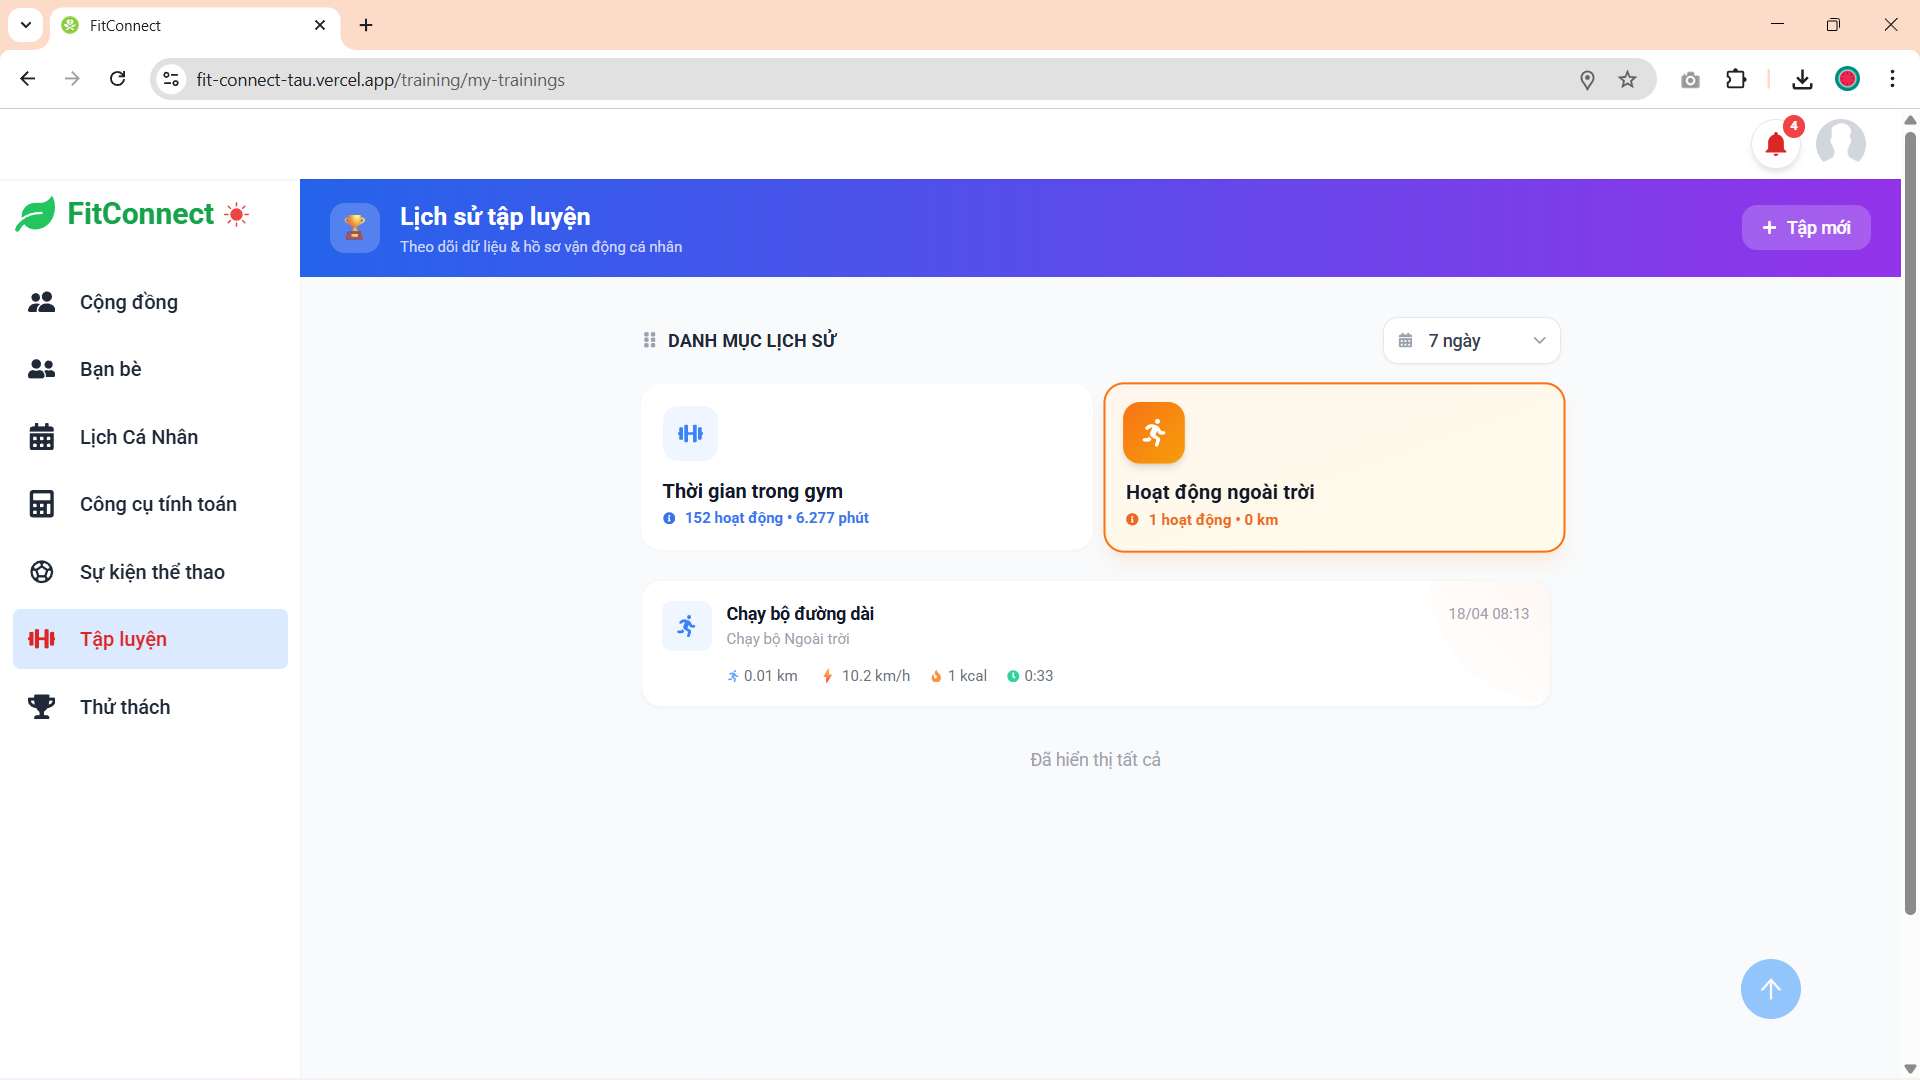
\includegraphics[width=0.60\textwidth]{Images/IMG/nhom5/lichsusaukhitapluyenchayboxong.png}
    \caption{Hệ thống hiển thị lịch sử hoạt động ngoài trời với thông số chi tiết}
    \label{fig:impl_train_history_outdoor}
\end{figure}

\end{itemize}

\subsection{Nhóm tính năng Lịch cá nhân và Thông báo}
\label{subsec:impl_calendar_notification}

Nhóm tính năng Lịch cá nhân và Thông báo giúp người dùng quản lý lịch hoạt động theo thời gian, theo dõi các đầu việc quan trọng trong ngày, đồng thời tiếp nhận các tương tác và cập nhật hệ thống theo thời gian thực. Lịch cá nhân đóng vai trò trung tâm tổng hợp các nguồn dữ liệu từ lịch tập luyện đã lưu, sự kiện thể thao đã tham gia và thử thách đang theo đuổi; trong khi trung tâm thông báo hỗ trợ phân loại, đánh dấu đã đọc, điều hướng nhanh đến nội dung liên quan và quản lý thông báo thuận tiện ngay trên thanh tiêu đề.

\subsubsection{Luồng thao tác trên Lịch cá nhân}
\begin{itemize}
    \item Người dùng truy cập mục ``Lịch Cá Nhân'' từ thanh điều hướng bên trái. Hệ thống hiển thị giao diện lịch tổng quan, kết hợp các hoạt động theo mốc thời gian gồm: sự kiện thể thao, lịch tập luyện và thử thách. Tại phần điều khiển, người dùng có thể chuyển nhanh về ``Hôm nay'', điều hướng tháng/tuần kế tiếp, đồng thời bật/tắt từng nhóm dữ liệu để tập trung vào nội dung cần theo dõi.

\begin{figure}[H]
    \centering
    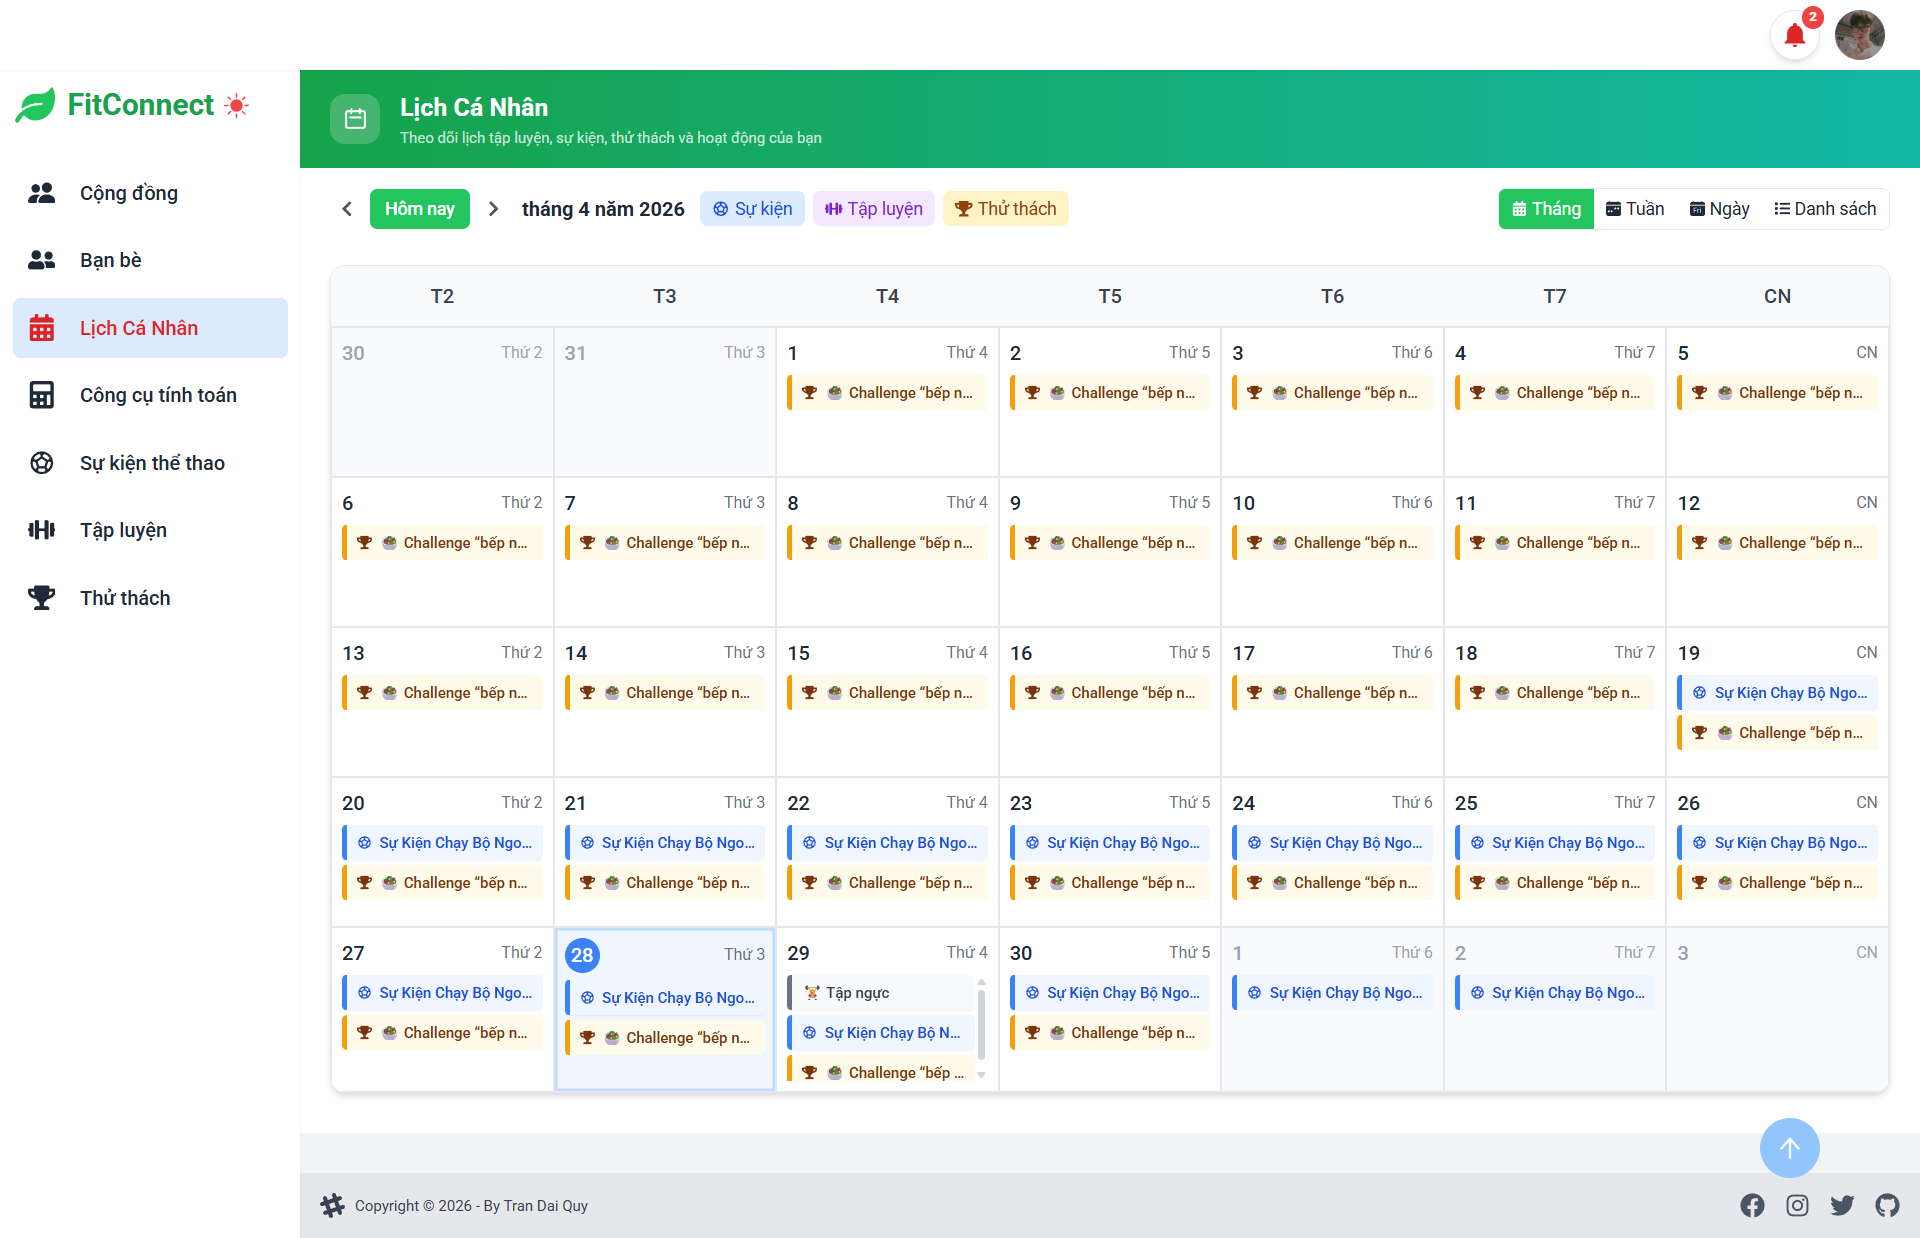
\includegraphics[width=0.60\textwidth]{Images/IMG/nhom8/tranglichcanhan.png}
    \caption{Hệ thống hiển thị trang Lịch cá nhân với bộ lọc theo loại hoạt động}
    \label{fig:impl_cal_main}
\end{figure}


    \item Ở chế độ ``Tháng'', người dùng quan sát toàn bộ kế hoạch trong tháng hiện tại dưới dạng lưới ngày. Mỗi ô ngày hiển thị rút gọn các hoạt động chính và cho phép nhấn để xem nhanh hoạt động phát sinh trong ngày đó, phù hợp cho việc theo dõi tổng quan và phát hiện các ngày có mật độ hoạt động cao.

\begin{figure}[H]
    \centering
    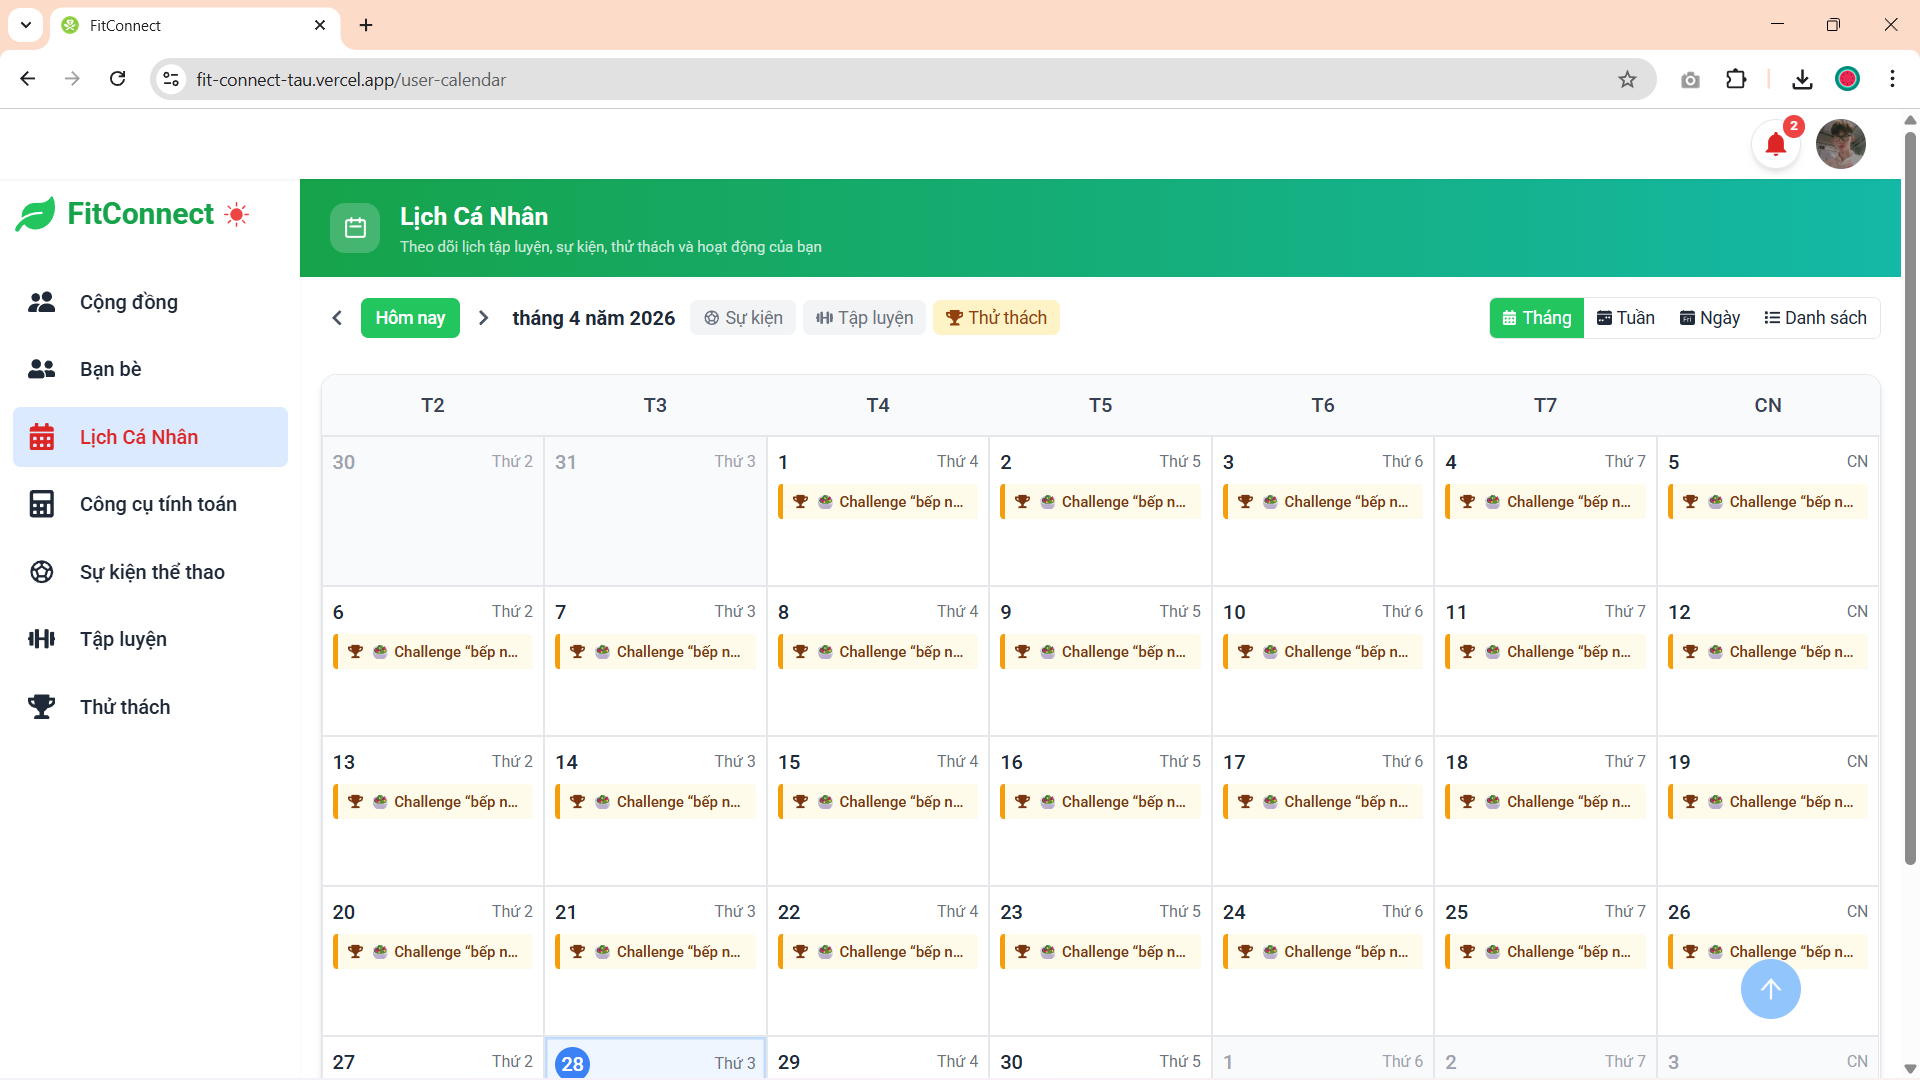
\includegraphics[width=0.60\textwidth]{Images/IMG/nhom8/chedothangtrangtongquan.png}
    \caption{Người dùng theo dõi lịch hoạt động ở chế độ Tháng}
    \label{fig:impl_cal_month}
\end{figure}


    \item Người dùng có thể chuyển sang các chế độ ``Tuần'', ``Ngày'' và ``Danh sách'' để xem lịch theo mức độ chi tiết khác nhau. Chế độ Tuần và Ngày hiển thị timeline theo giờ giúp quản lý khung thời gian tập luyện/sự kiện cụ thể; chế độ Danh sách gom sự kiện theo ngày, phù hợp khi cần quét nhanh toàn bộ hoạt động trong tháng.

\begin{figure}[H]
    \centering
    \begin{subfigure}[b]{0.30\textwidth}
        \centering
        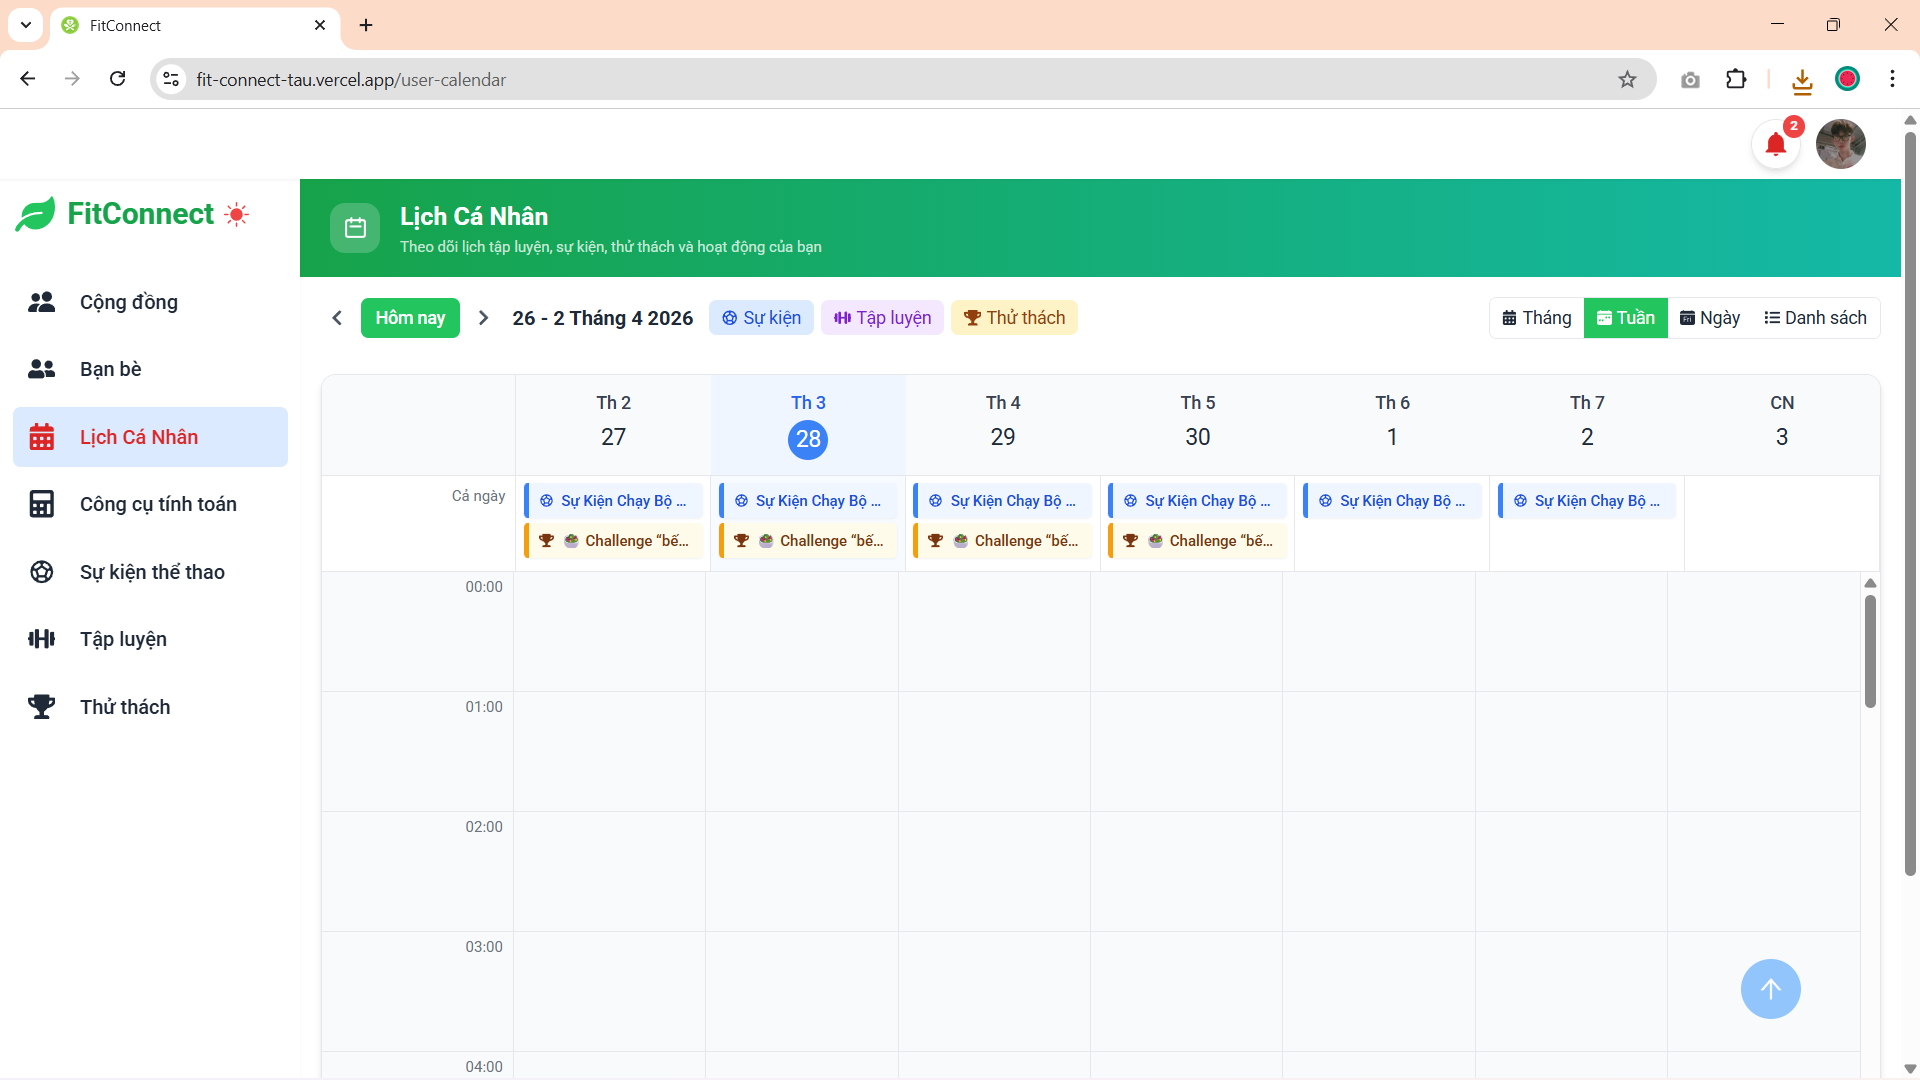
\includegraphics[width=\textwidth]{Images/IMG/nhom8/chedotuan.png}
        \caption{Hệ thống hiển thị lịch cá nhân ở chế độ Tuần theo khung giờ}
        \label{fig:impl_cal_week}
    \end{subfigure}
    \hfill
    \begin{subfigure}[b]{0.30\textwidth}
        \centering
        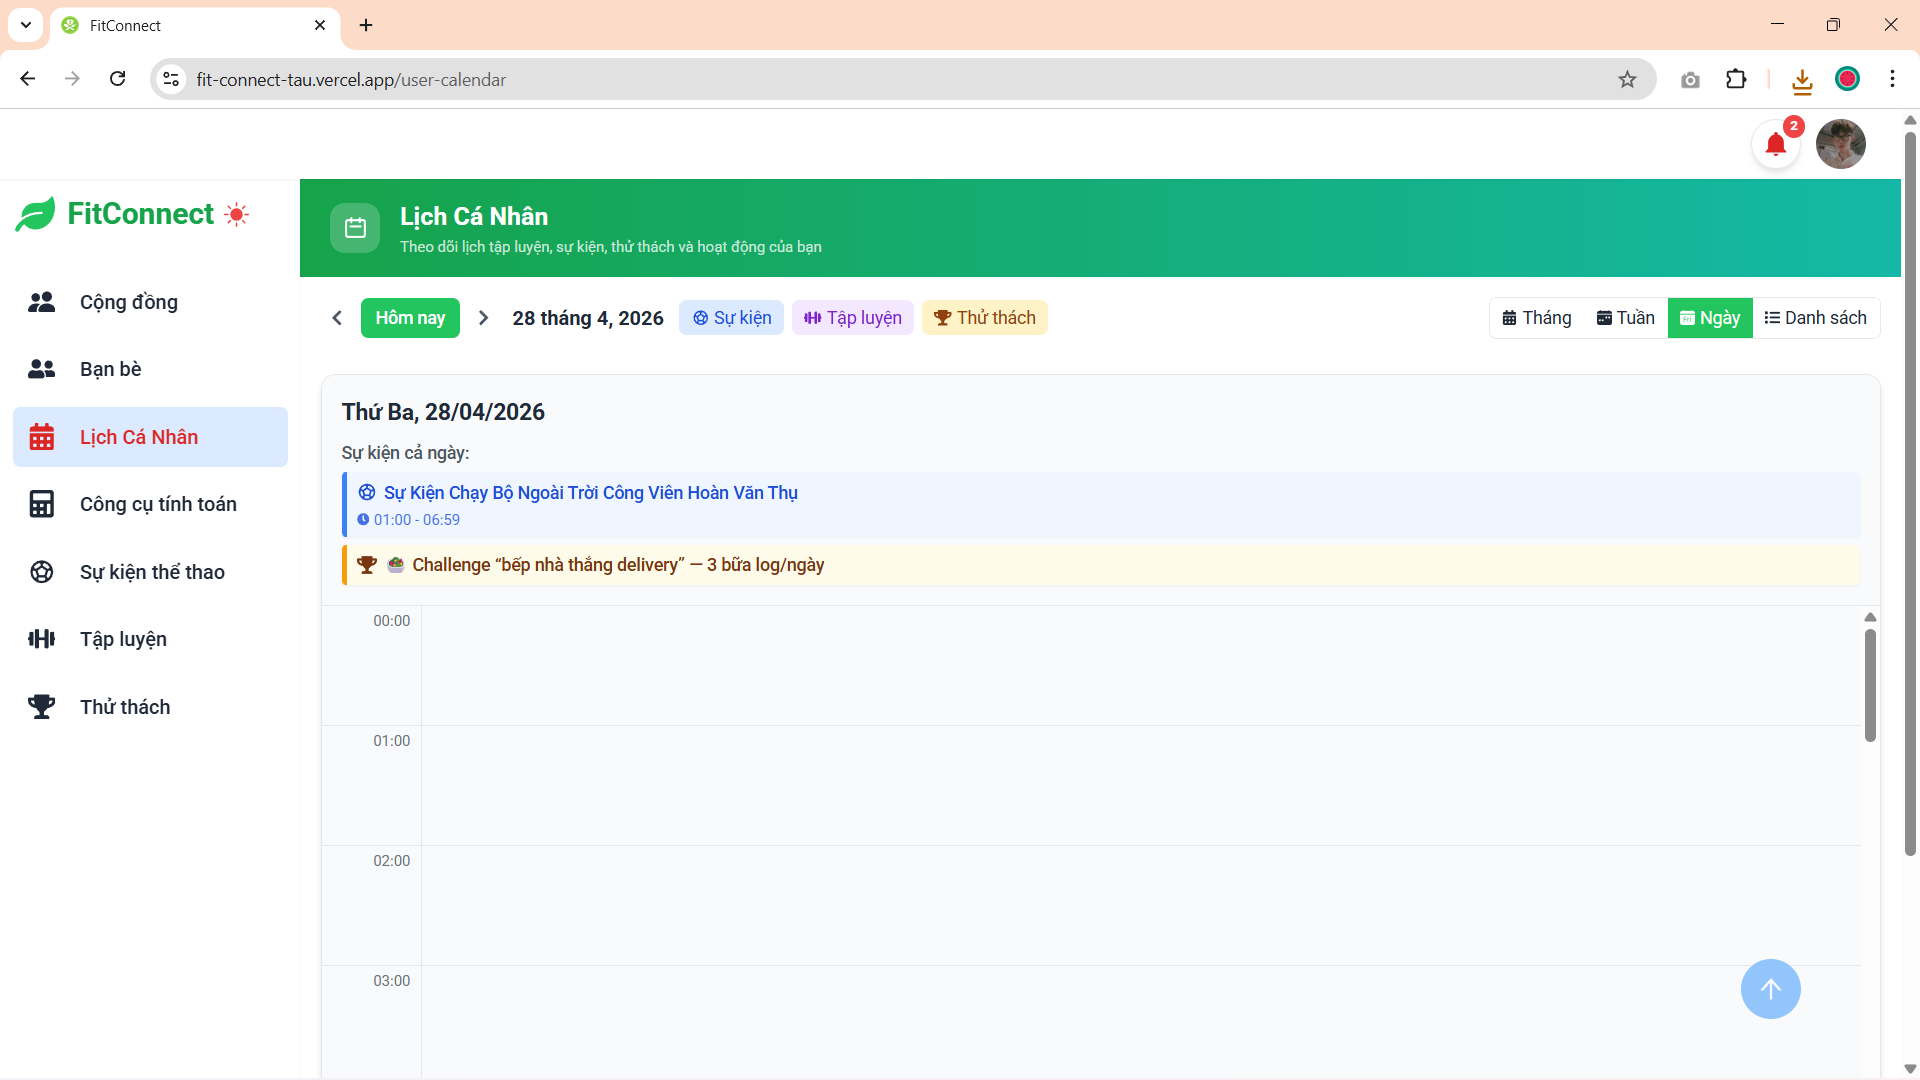
\includegraphics[width=\textwidth]{Images/IMG/nhom8/chedongay.png}
        \caption{Hệ thống hiển thị lịch cá nhân ở chế độ Ngày}
        \label{fig:impl_cal_day}
    \end{subfigure}
    \hfill
    \begin{subfigure}[b]{0.30\textwidth}
        \centering
        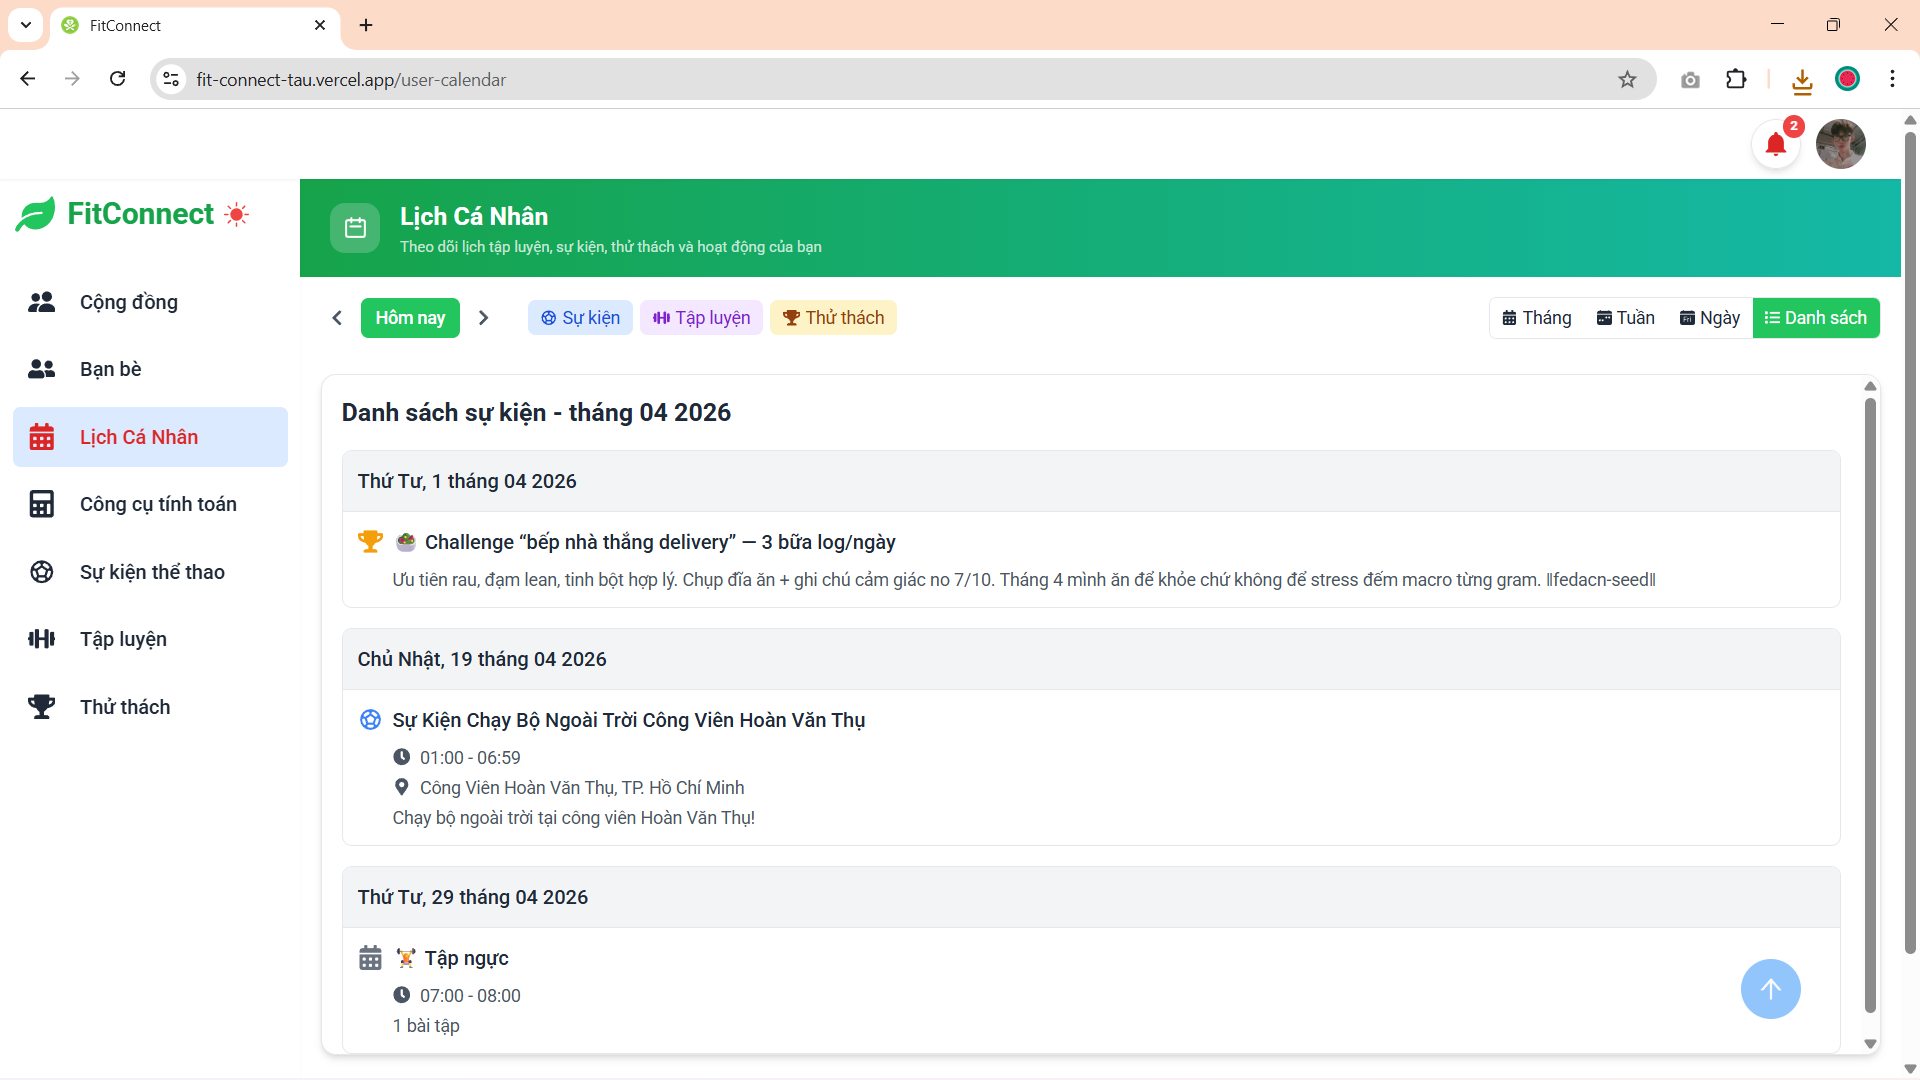
\includegraphics[width=\textwidth]{Images/IMG/nhom8/chedodanhsach.png}
        \caption{Hệ thống hiển thị lịch cá nhân ở chế độ Danh sách}
        \label{fig:impl_cal_agenda}
    \end{subfigure}
\end{figure}


    \item Khi nhấn vào một hoạt động cụ thể trên lịch, hệ thống mở modal chi tiết theo từng ngữ cảnh. Với sự kiện thể thao, người dùng xem được loại sự kiện, thời gian, địa điểm, trạng thái tham gia và thông tin tổ chức.

\begin{figure}[H]
    \centering
    
\includegraphics[width=0.60\textwidth]{Images/IMG/nhom8/chitietsukien.png}
    \caption{Hệ thống hiển thị modal chi tiết sự kiện thể thao từ Lịch cá nhân}
    \label{fig:impl_cal_event_detail}
\end{figure}


    \item Tương tự, khi chọn một thử thách trên lịch, hệ thống hiển thị thông tin tổng quan thử thách gồm trạng thái, mô tả và điều hướng nhanh tới trang thử thách để tiếp tục theo dõi tiến độ.

\begin{figure}[H]
    \centering
    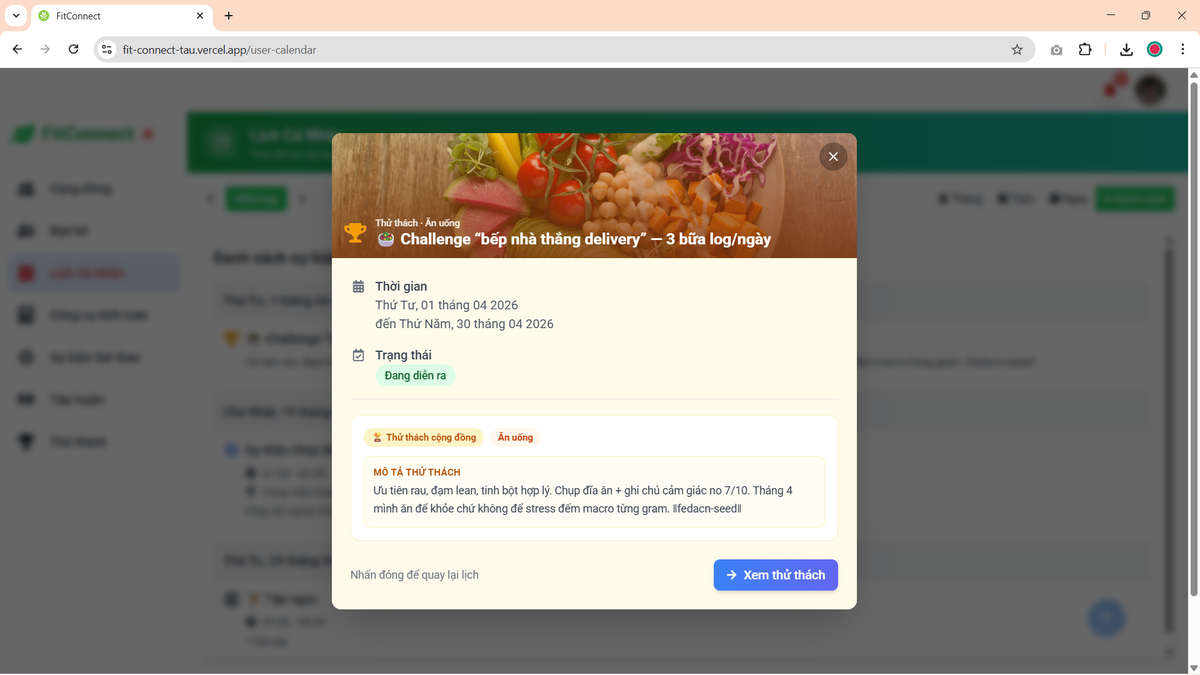
\includegraphics[width=0.60\textwidth]{Images/IMG/nhom8/chitietthuthach.png}
    \caption{Hệ thống hiển thị modal chi tiết thử thách từ Lịch cá nhân}
    \label{fig:impl_cal_challenge_detail}
\end{figure}


    \item Với lịch tập luyện đã lưu, modal chi tiết hiển thị danh sách bài tập, số set và thông tin nhắc nhở; người dùng có thể nhấn ``Tập ngay'' để chuyển trực tiếp sang màn hình tập luyện, giúp rút ngắn thao tác thực thi kế hoạch trong ngày.

\begin{figure}[H]
    \centering
    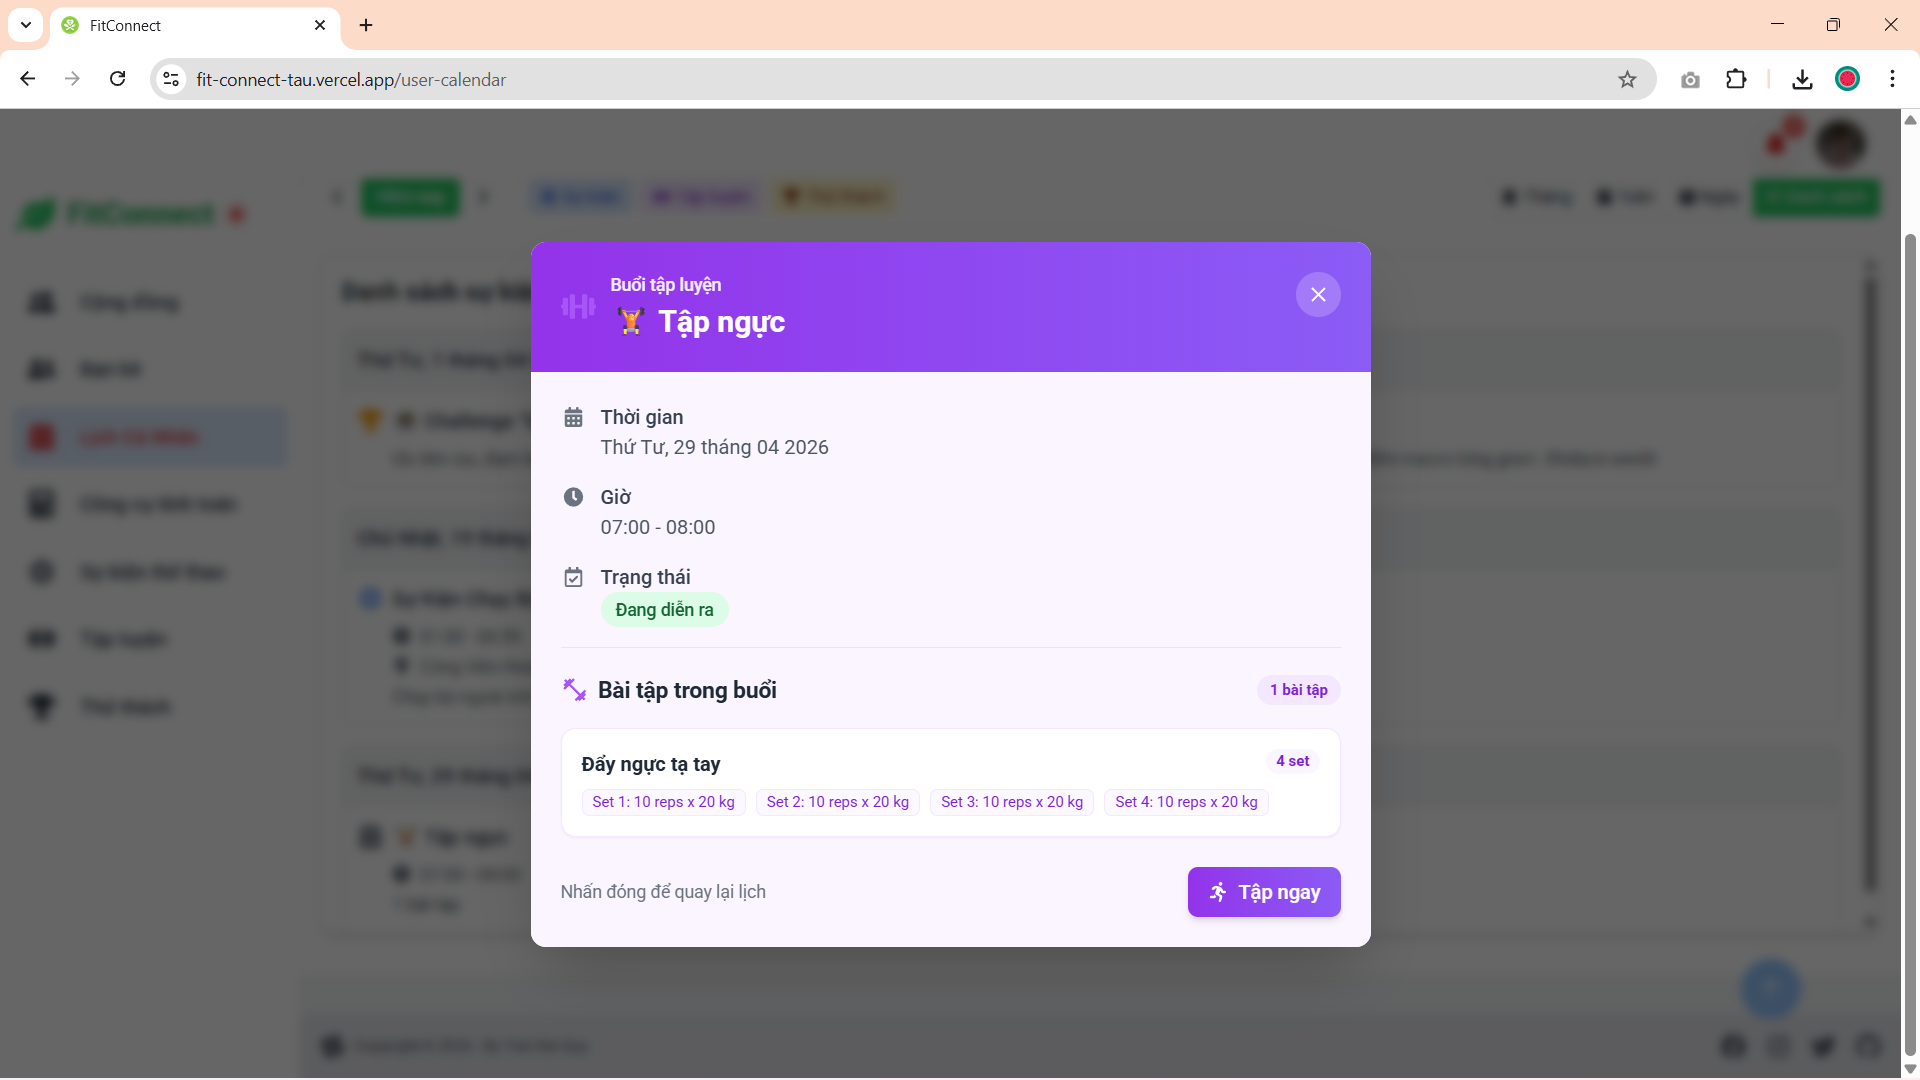
\includegraphics[width=0.60\textwidth]{Images/IMG/nhom8/chitiettapluyen.png}
    \caption{Hệ thống hiển thị modal chi tiết lịch tập luyện và điều hướng tập ngay}
    \label{fig:impl_cal_workout_detail}
\end{figure}


    \item Khi cần theo dõi nhanh công việc trong ngày hiện tại, người dùng nhấn ``Hôm nay'' để đưa lịch về mốc hiện tại và xem các hoạt động phát sinh trong ngày, bao gồm sự kiện, thử thách và buổi tập đã lên lịch.

\begin{figure}[H]
    \centering
    \begin{subfigure}[b]{0.30\textwidth}
        \centering
        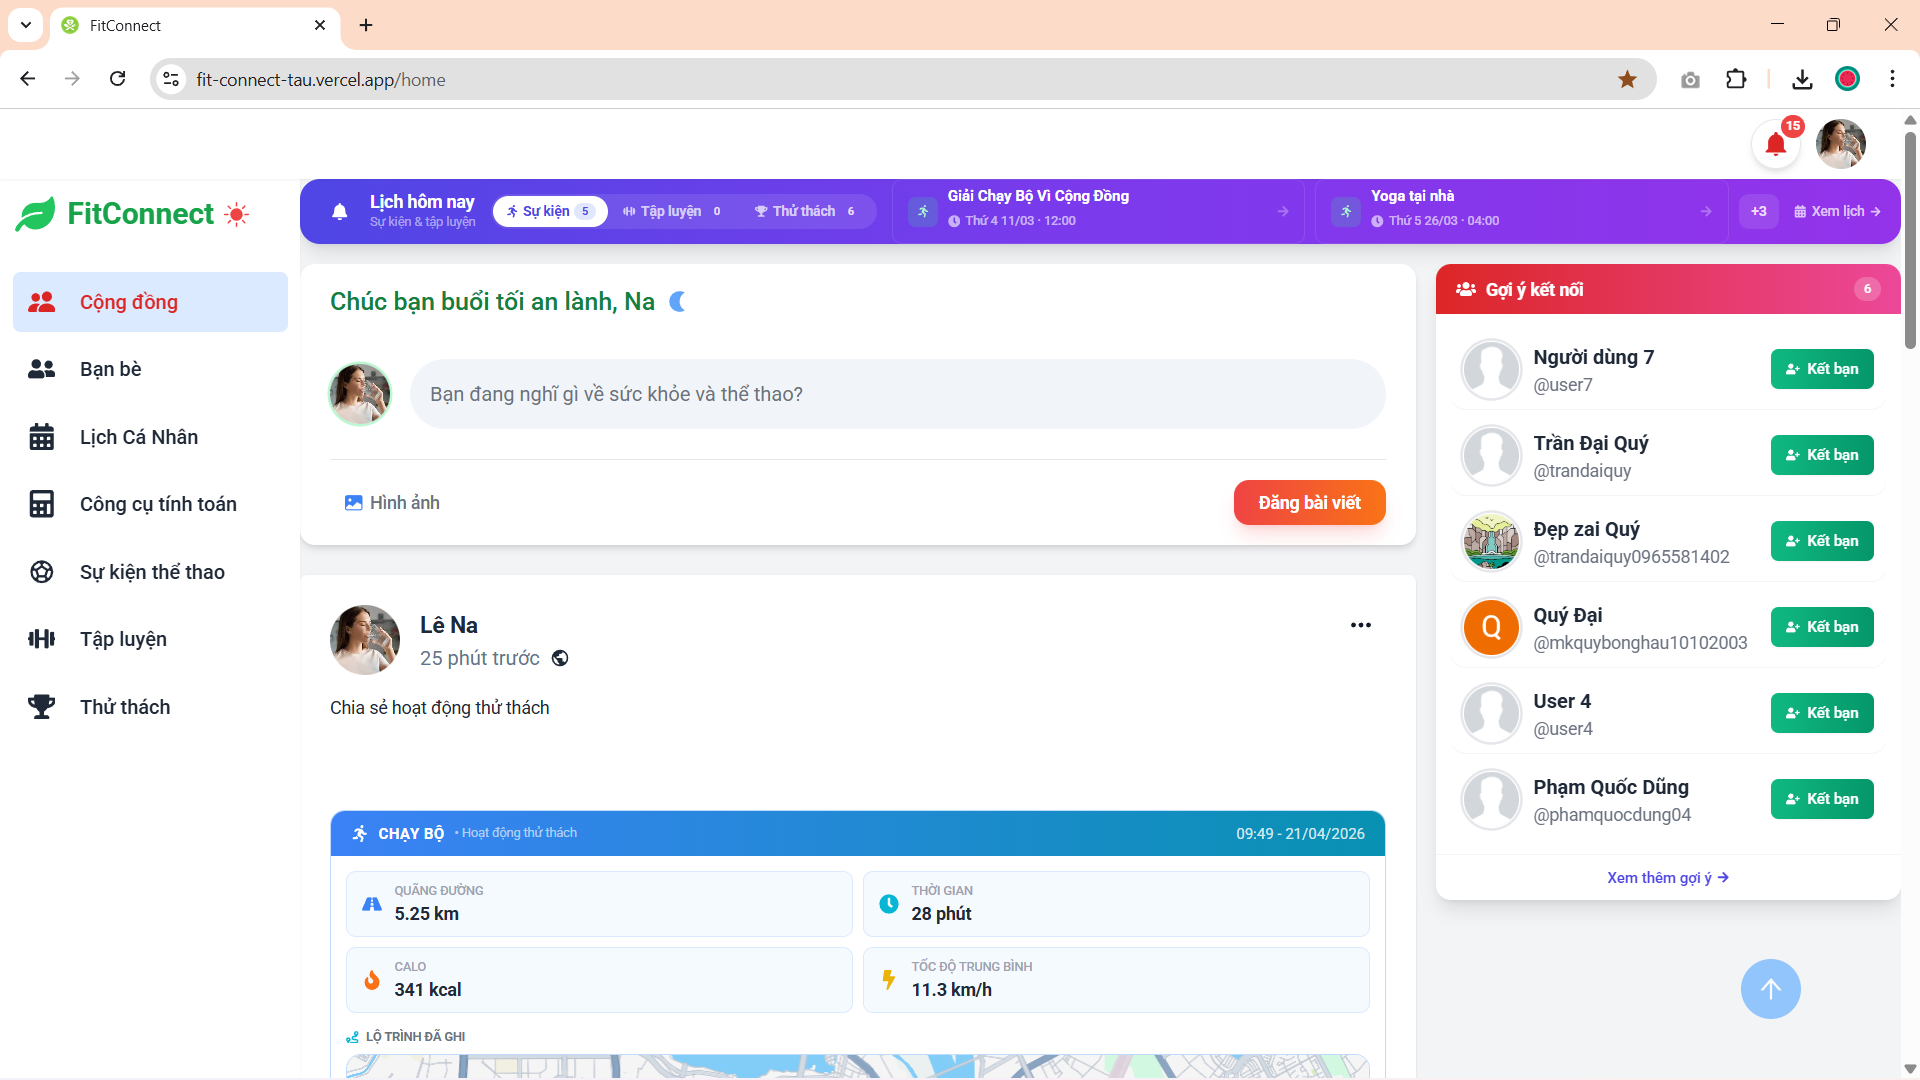
\includegraphics[width=\textwidth]{Images/IMG/nhom8/lichhomnaysukien.png}
        \caption{Người dùng theo dõi hoạt động sự kiện trong ngày hiện tại}
        \label{fig:impl_cal_today_event}
    \end{subfigure}
    \hfill
    \begin{subfigure}[b]{0.30\textwidth}
        \centering
        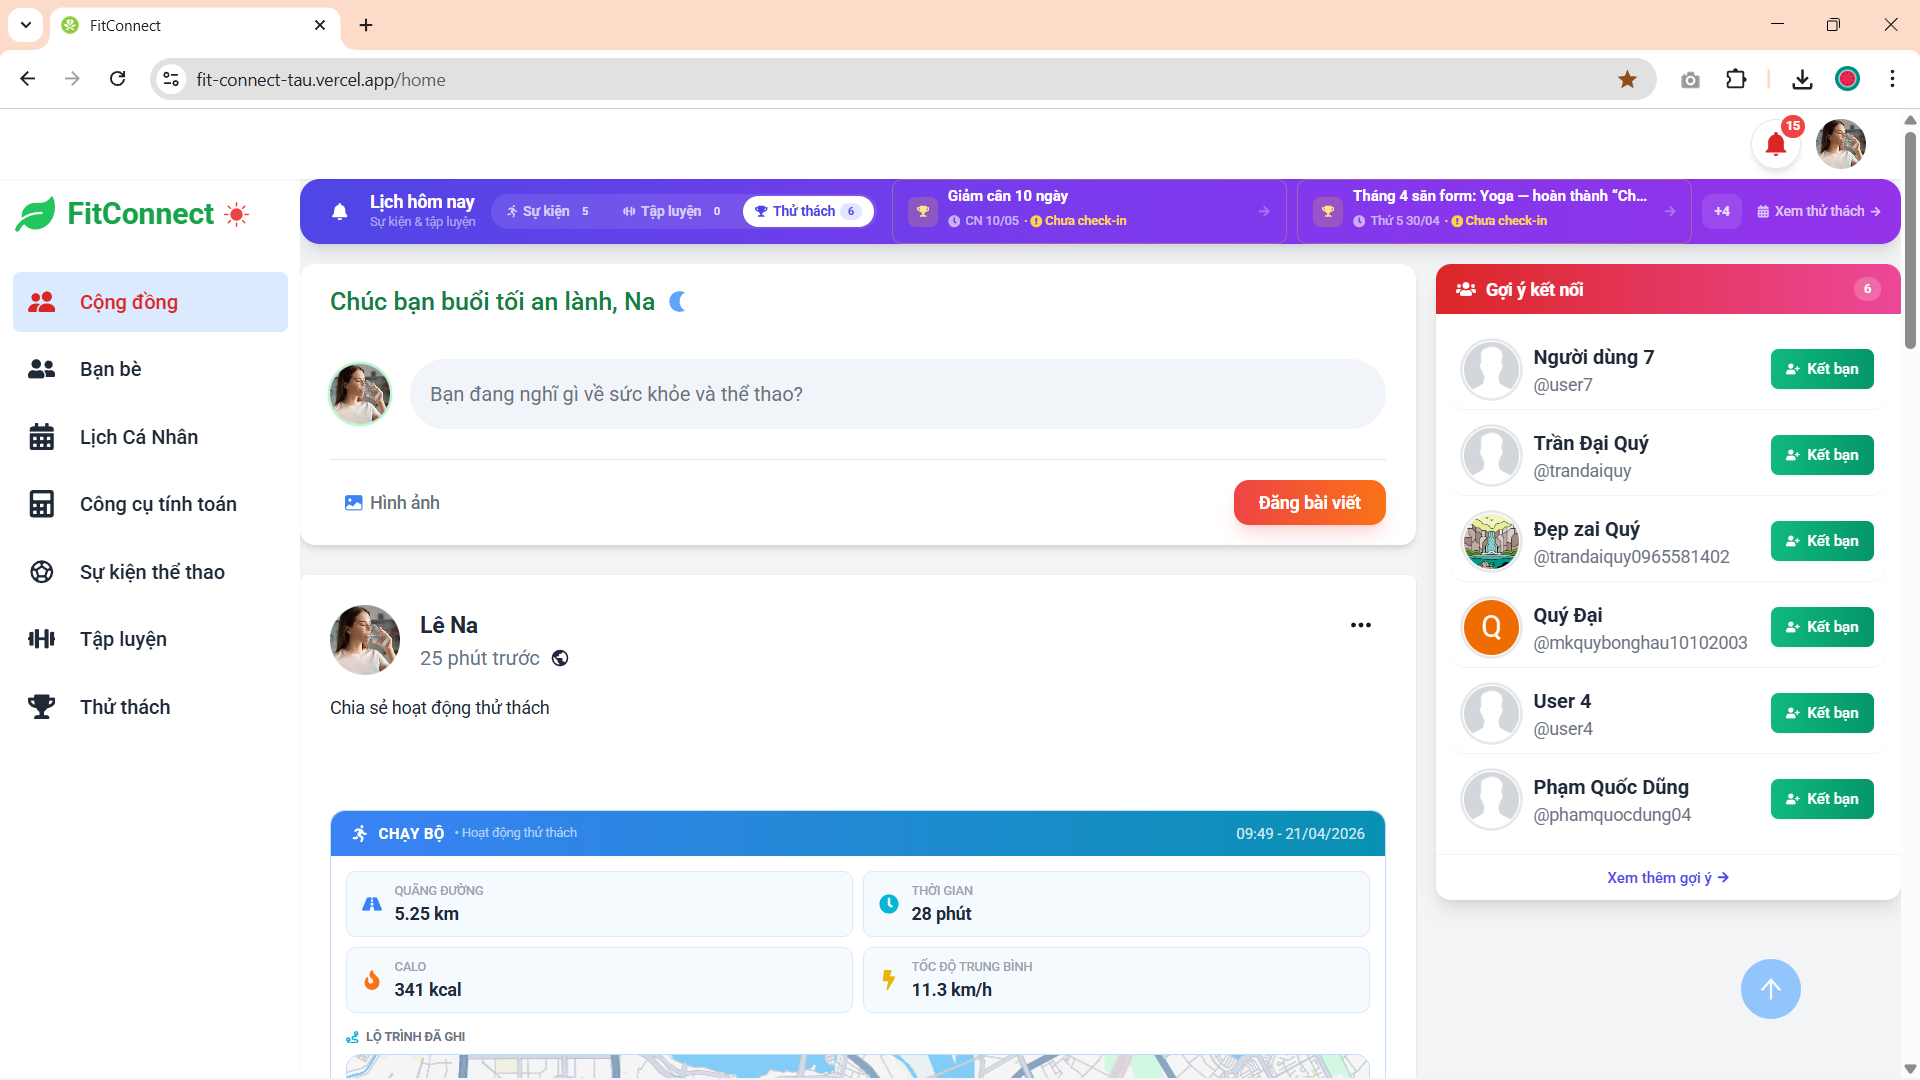
\includegraphics[width=\textwidth]{Images/IMG/nhom8/lichhomnaythuthach.png}
        \caption{Người dùng theo dõi hoạt động thử thách trong ngày hiện tại}
        \label{fig:impl_cal_today_challenge}
    \end{subfigure}
    \hfill
    \begin{subfigure}[b]{0.30\textwidth}
        \centering
        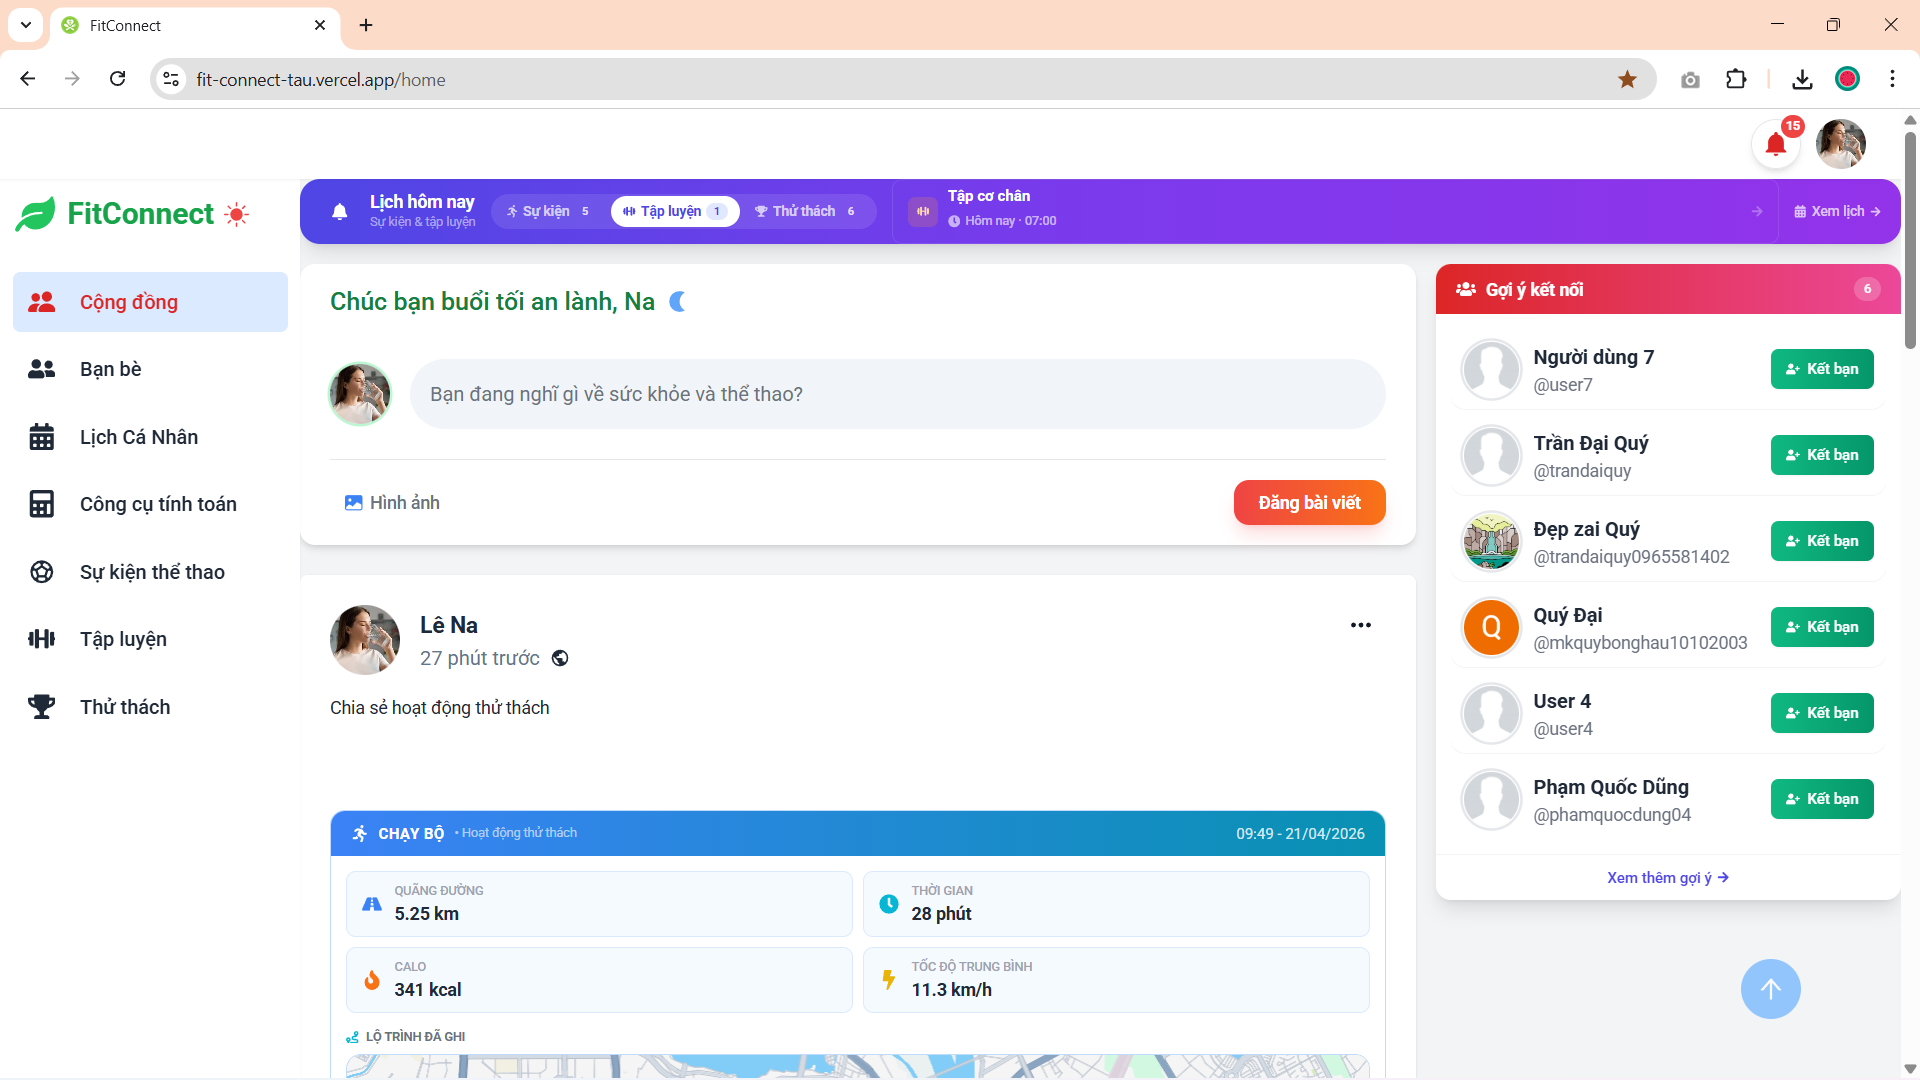
\includegraphics[width=\textwidth]{Images/IMG/nhom8/lichhomnaytapluyen.png}
        \caption{Người dùng theo dõi lịch tập luyện trong ngày hiện tại}
        \label{fig:impl_cal_today_workout}
    \end{subfigure}
\end{figure}

\end{itemize}

\subsubsection{Luồng thao tác trên trung tâm Thông báo}
\begin{itemize}
    \item Từ biểu tượng chuông, người dùng mở trung tâm thông báo với ba tab: \textbf{Tất cả} (tổng hợp toàn bộ), \textbf{Tương tác} (kết bạn, mời tham gia, bình luận) và \textbf{Hệ thống} (cảnh báo/cập nhật nền tảng). Người dùng có thể đánh dấu đã đọc, xóa thông báo và nhấn để điều hướng nhanh đến nội dung liên quan.

\begin{figure}[H]
    \centering
    \begin{subfigure}[b]{0.30\textwidth}
        \centering
        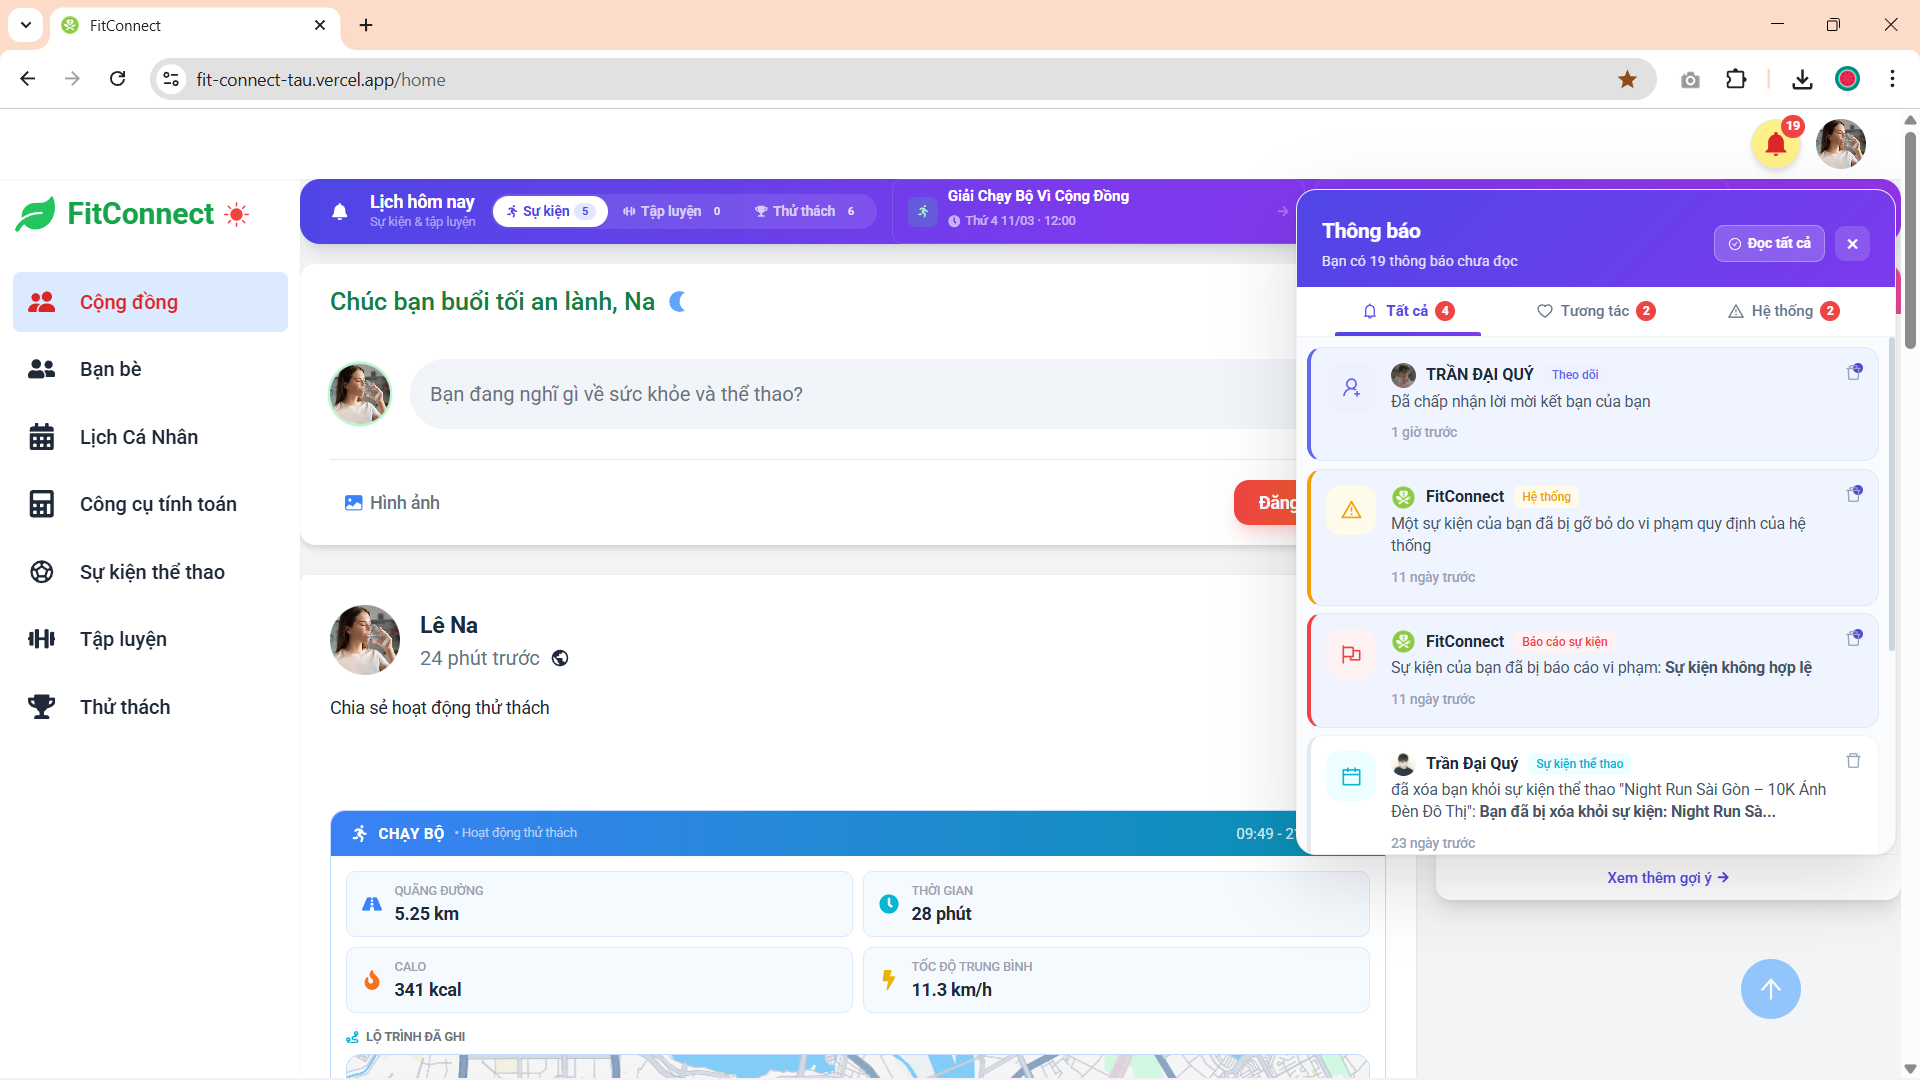
\includegraphics[width=\textwidth]{Images/IMG/nhom8/thongbaotatca.png}
        \caption{Tab Tất cả}
        \label{fig:impl_noti_all}
    \end{subfigure}
    \hfill
    \begin{subfigure}[b]{0.30\textwidth}
        \centering
        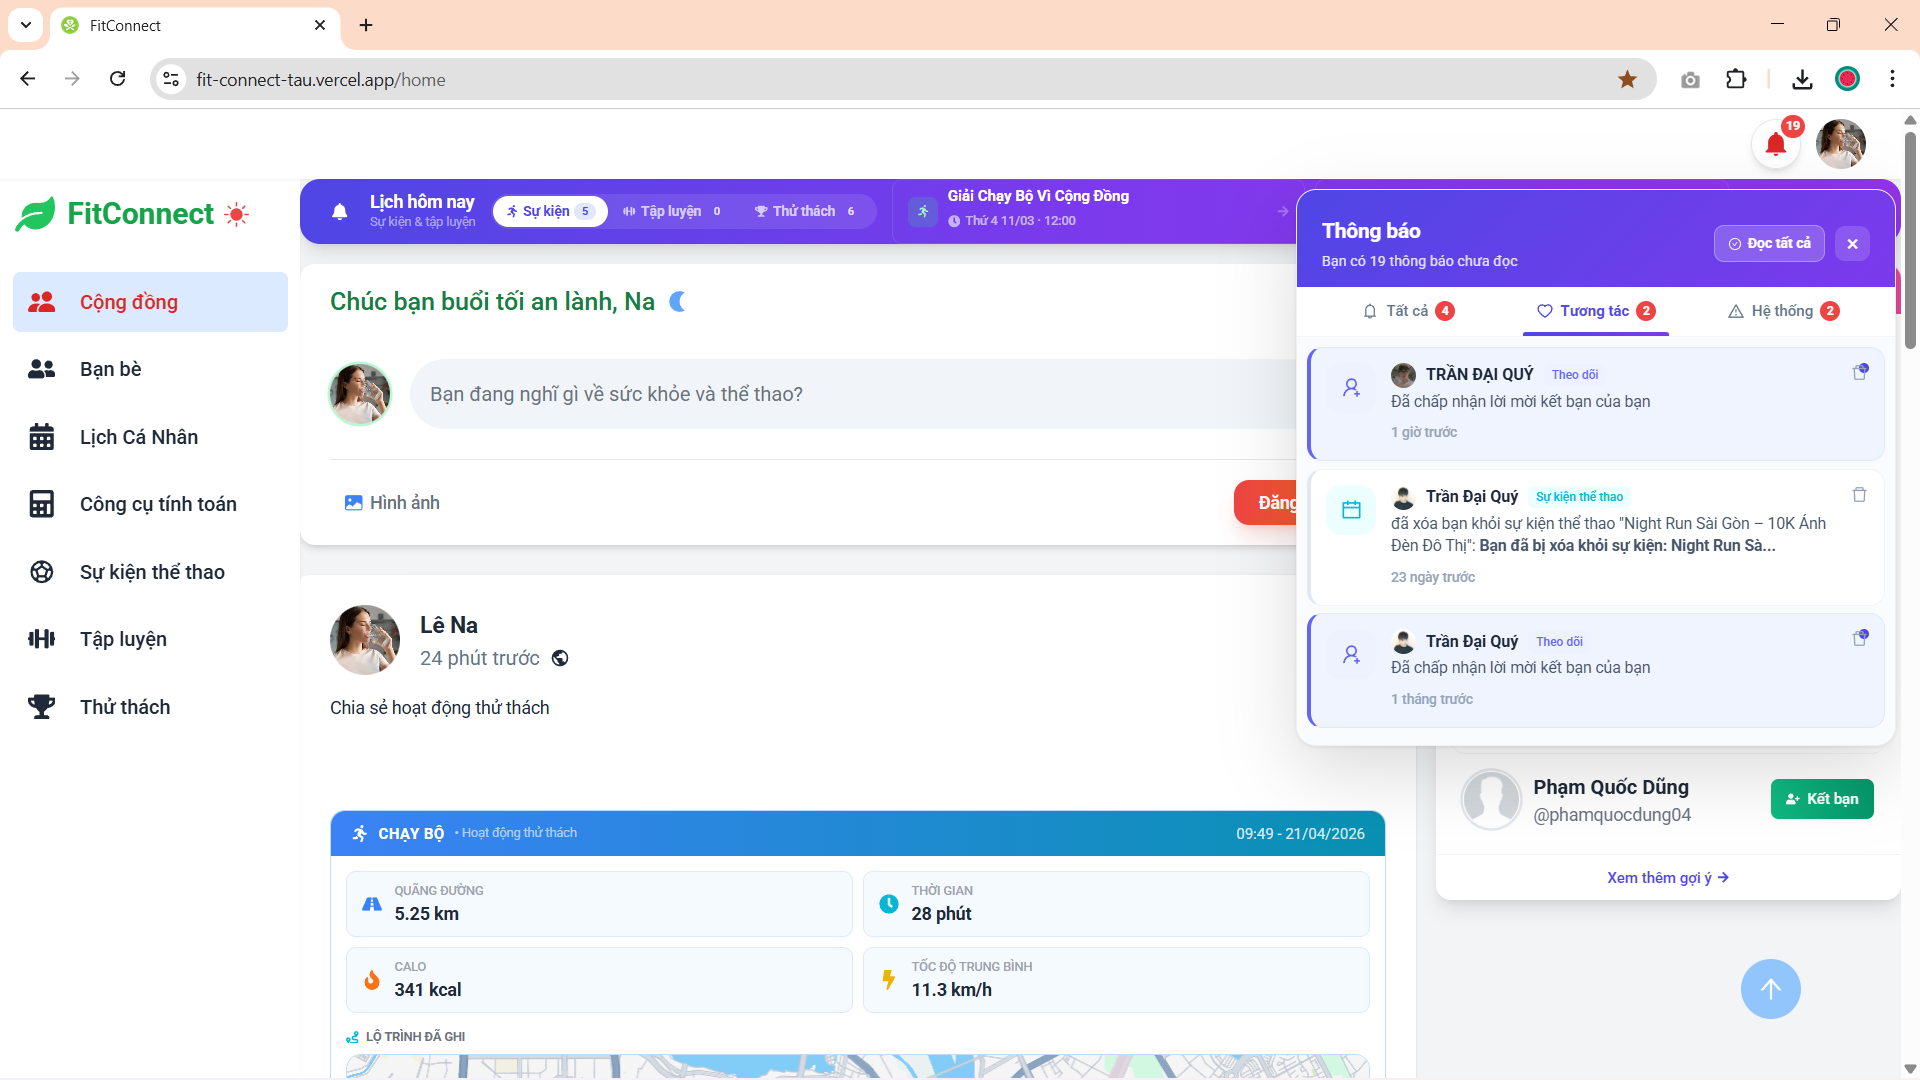
\includegraphics[width=\textwidth]{Images/IMG/nhom8/thongbaotuongtac.png}
        \caption{Tab Tương tác}
        \label{fig:impl_noti_social}
    \end{subfigure}
    \hfill
    \begin{subfigure}[b]{0.30\textwidth}
        \centering
        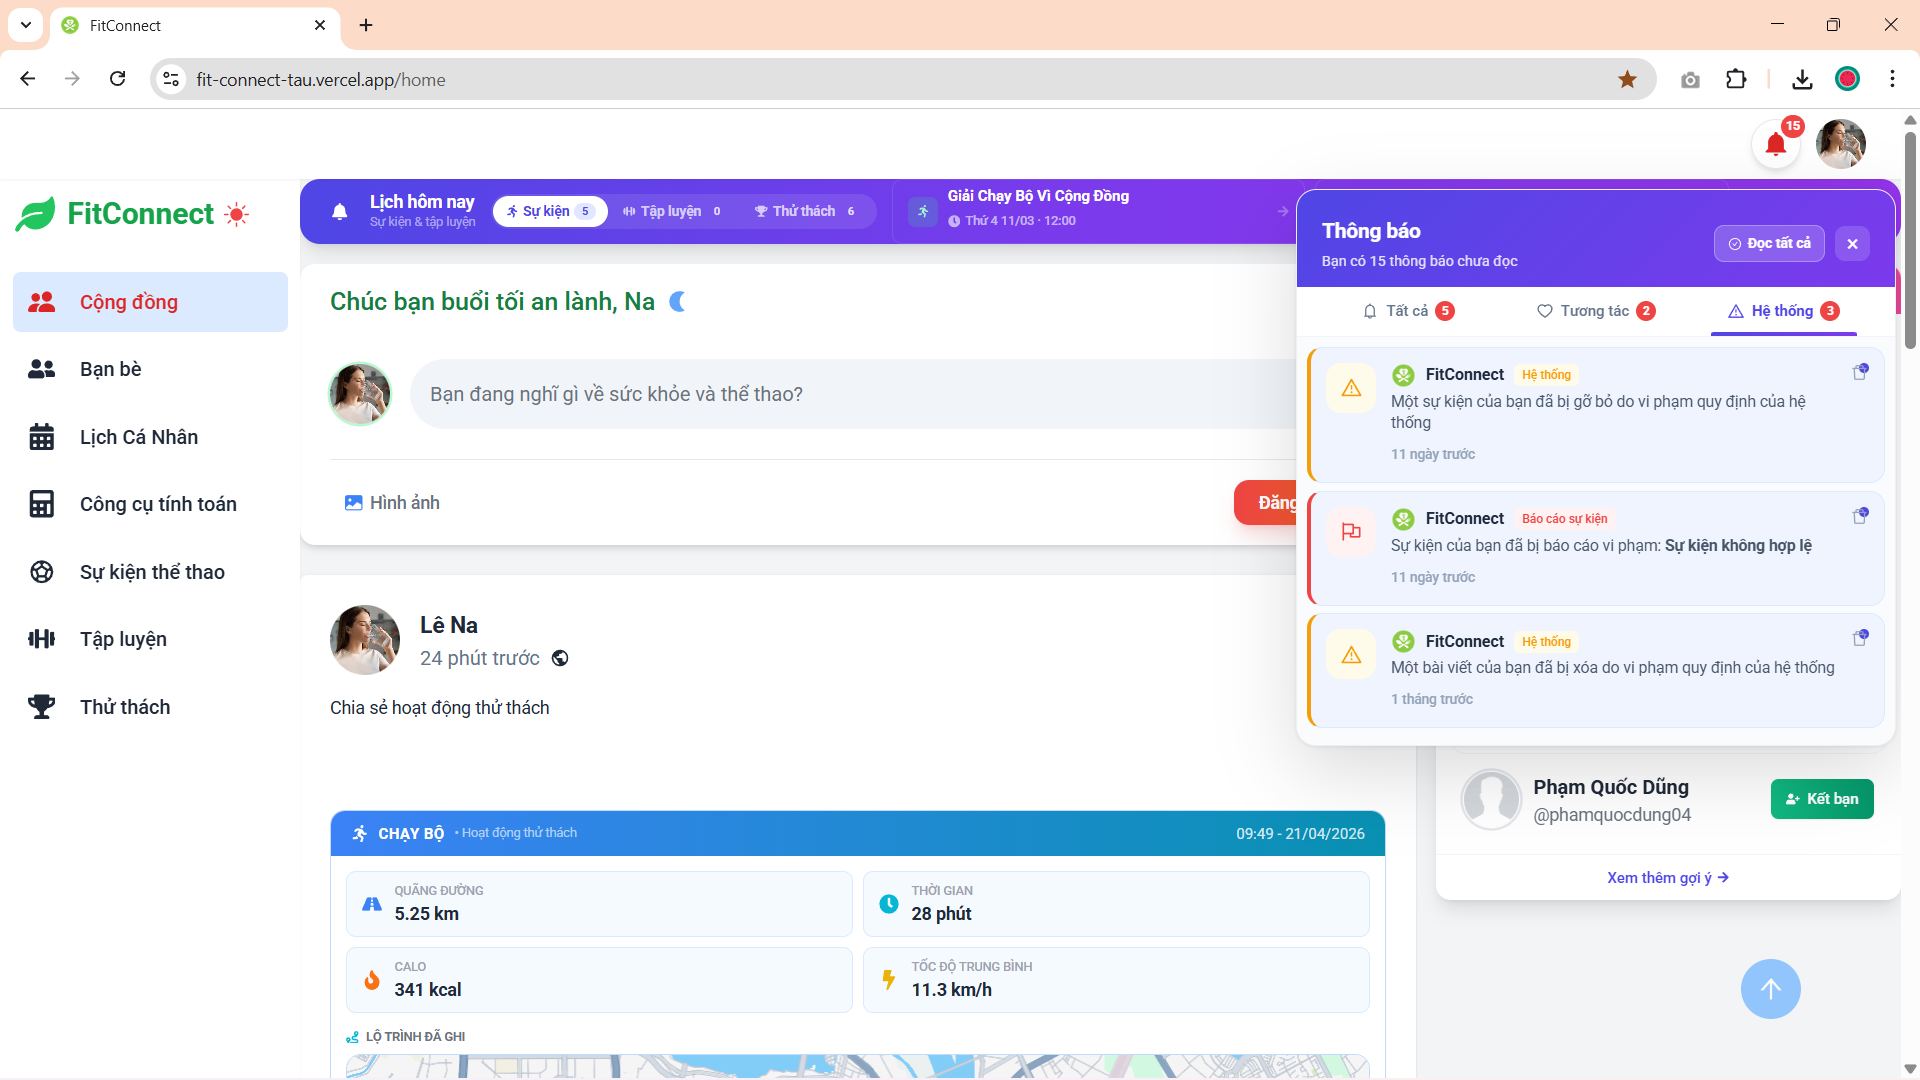
\includegraphics[width=\textwidth]{Images/IMG/nhom8/thongbaohethong.png}
        \caption{Tab Hệ thống}
        \label{fig:impl_noti_system}
    \end{subfigure}
    \vspace{0.3em}
    \caption{Trung tâm Thông báo với ba tab phân loại theo ngữ cảnh}
    \label{fig:impl_noti_center}
\end{figure}

\end{itemize}

\subsection{Nhóm tính năng Bạn bè}
\label{subsec:impl_friends}

Nhóm tính năng Bạn bè giúp người dùng xây dựng mạng lưới kết nối trong hệ thống, quản lý quan hệ theo dõi hai chiều và tăng tương tác thông qua lời mời tham gia hoạt động. Cơ chế cốt lõi của nhóm này dựa trên mô hình follow: khi hai người dùng theo dõi lẫn nhau thì được xem là bạn bè. Hệ thống đồng thời cung cấp danh sách gợi ý để người dùng mở rộng kết nối, kèm các thông báo thời gian thực cho những hành động quan trọng như gửi lời mời, chấp nhận kết bạn, và mời tham gia sự kiện/thử thách.

\subsubsection{Luồng thao tác quản lý bạn bè}
\begin{itemize}
    \item Người dùng truy cập trang Bạn bè, hệ thống hiển thị dashboard quản lý quan hệ gồm các khu vực chính: danh sách Bạn bè, Lời mời kết bạn, Người bạn theo dõi, Người theo dõi bạn, và khu vực Khám phá bạn bè để gợi ý kết nối mới.

\begin{figure}[H]
    \centering
    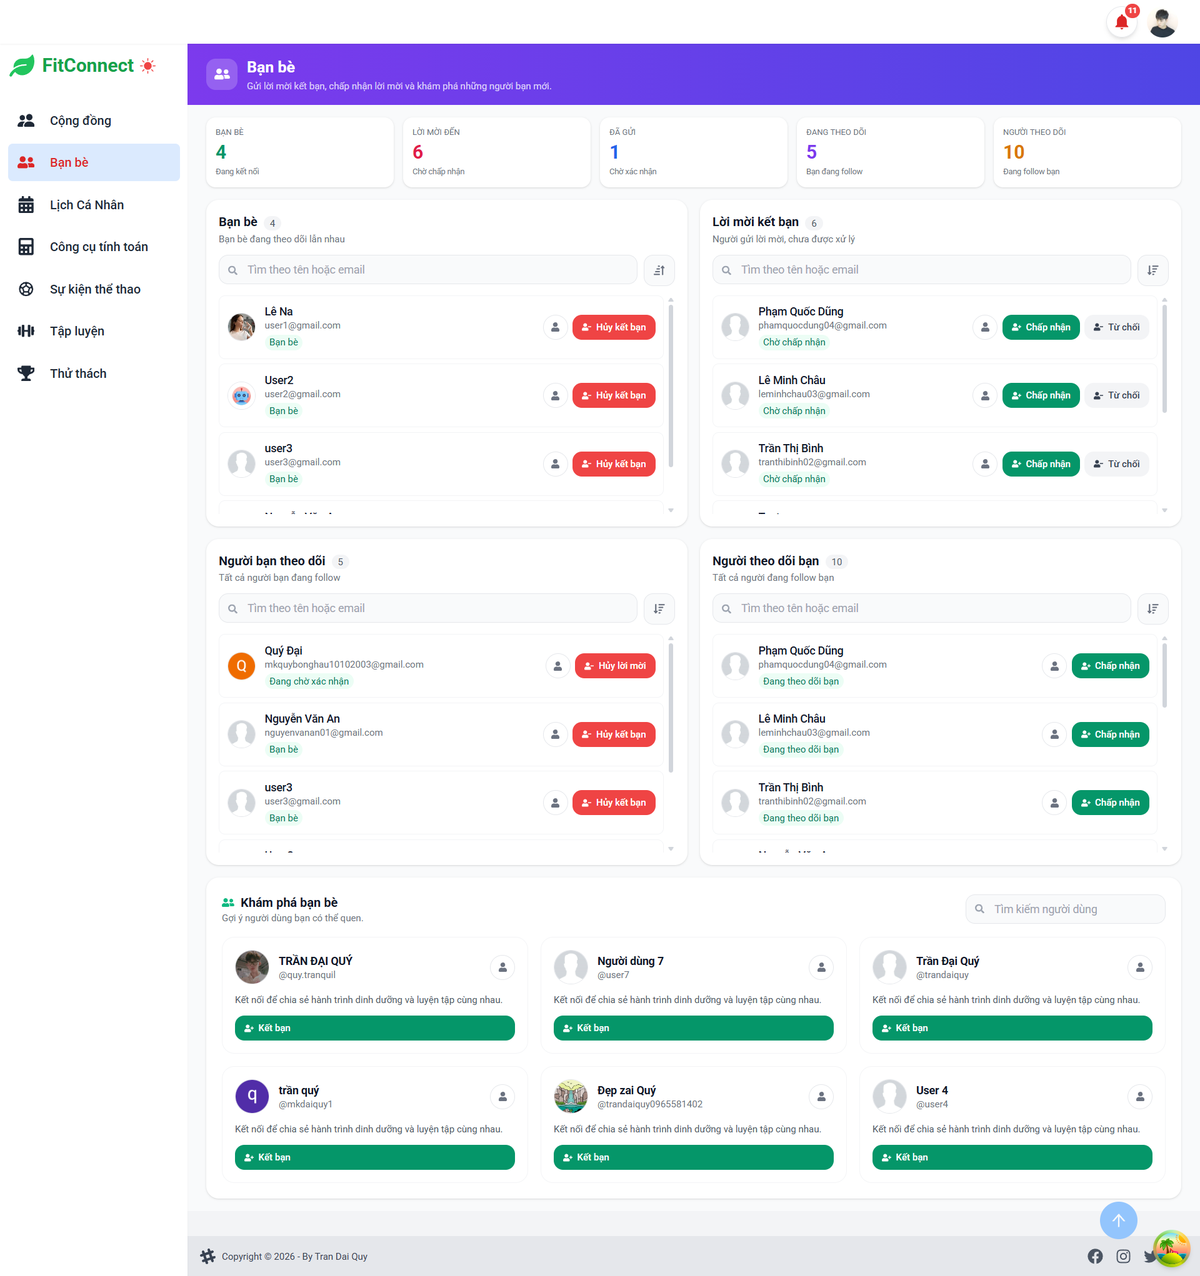
\includegraphics[width=0.60\textwidth]{Images/IMG/Nhom7/danhsachbanbe.png}
    \caption{Hệ thống hiển thị trang quản lý bạn bè với các danh sách quan hệ}
    \label{fig:impl_fr_dashboard}
\end{figure}


    \item Tại khu vực Lời mời kết bạn, người dùng có thể nhấn ``Chấp nhận'' để xác nhận lời mời. Sau khi chấp nhận, quan hệ giữa hai tài khoản chuyển thành bạn bè (theo dõi hai chiều), đồng thời hệ thống cập nhật số liệu thống kê liên quan trên trang.

\begin{figure}[H]
    \centering
    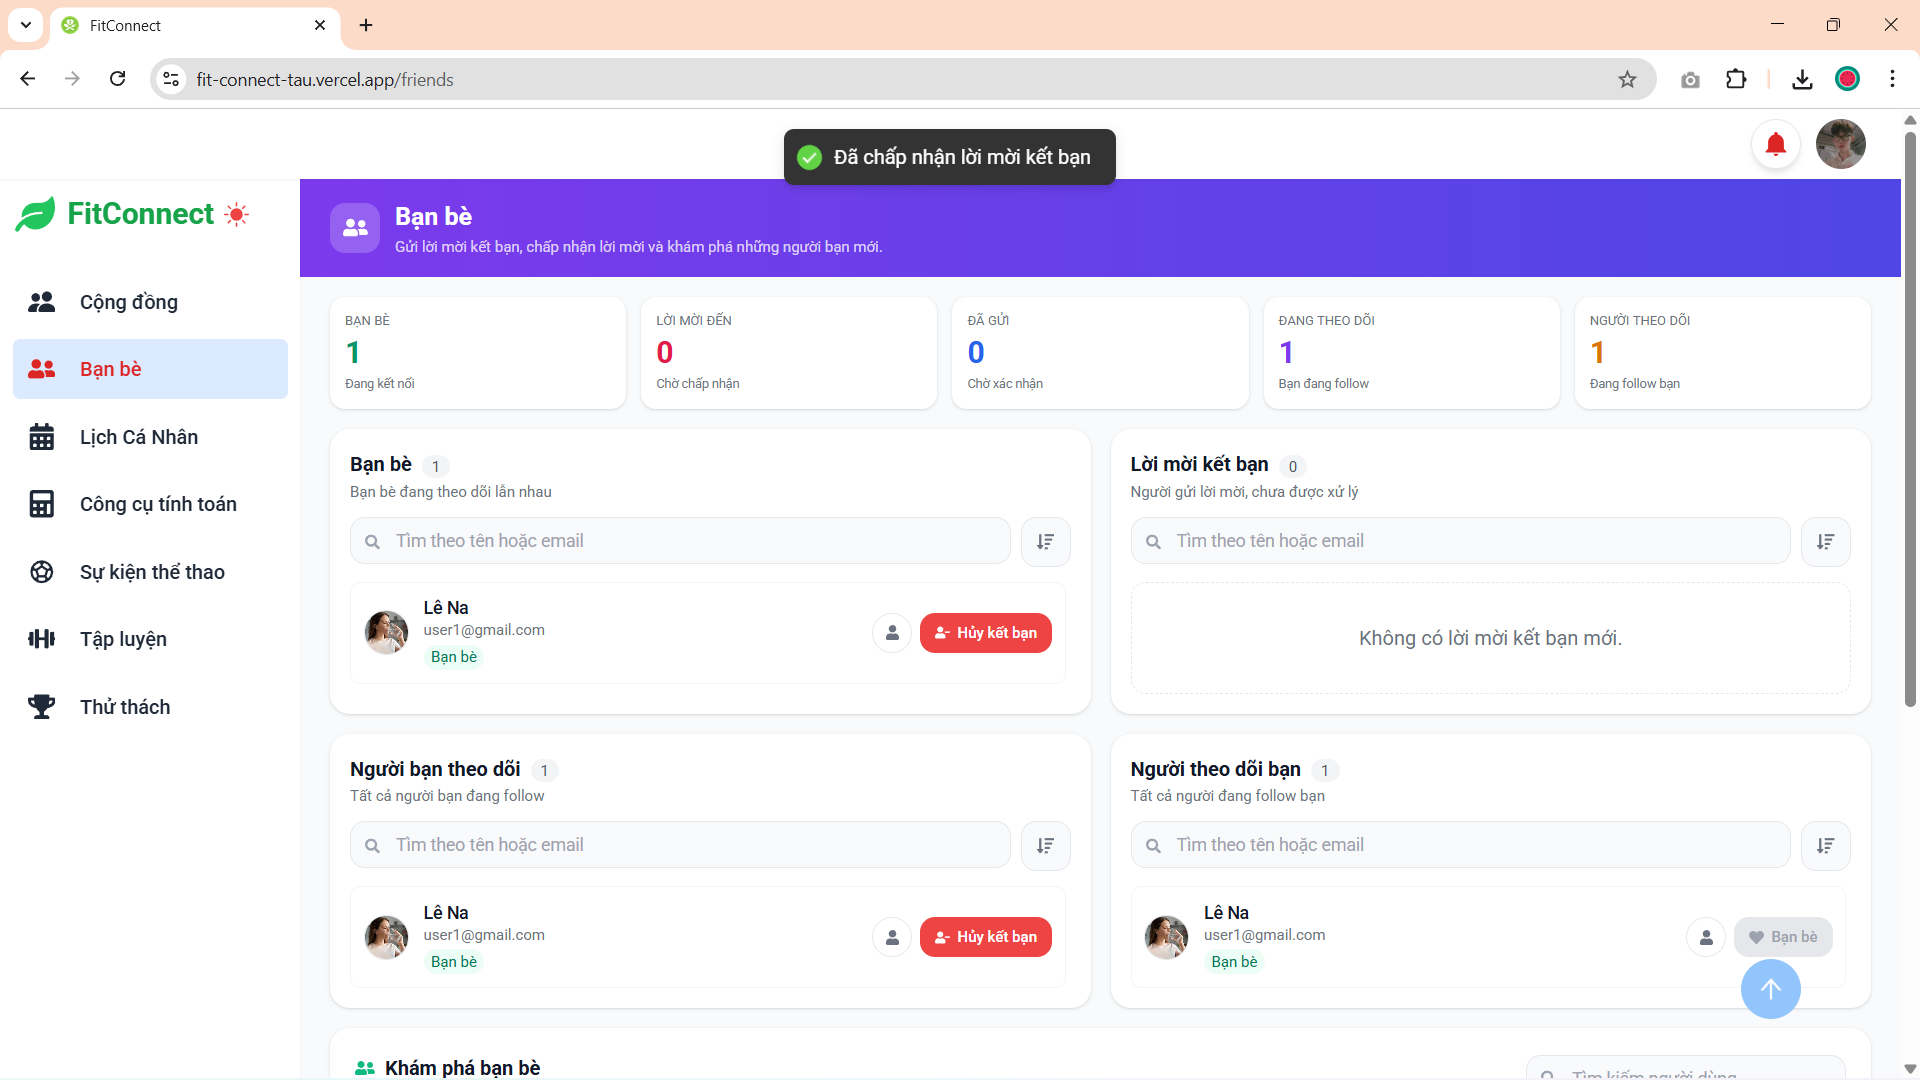
\includegraphics[width=0.60\textwidth]{Images/IMG/Nhom7/chapnhanketban.png}
    \caption{Người dùng thao tác chấp nhận lời mời kết bạn}
    \label{fig:impl_fr_accept}
\end{figure}


    \item Khi một người dùng gửi lời mời kết bạn, phía người nhận sẽ thấy thông báo tương ứng trong trung tâm thông báo. Người nhận có thể nhấn vào thông báo để điều hướng tới trang quản lý bạn bè và thực hiện xử lý lời mời.

\begin{figure}[H]
    \centering
    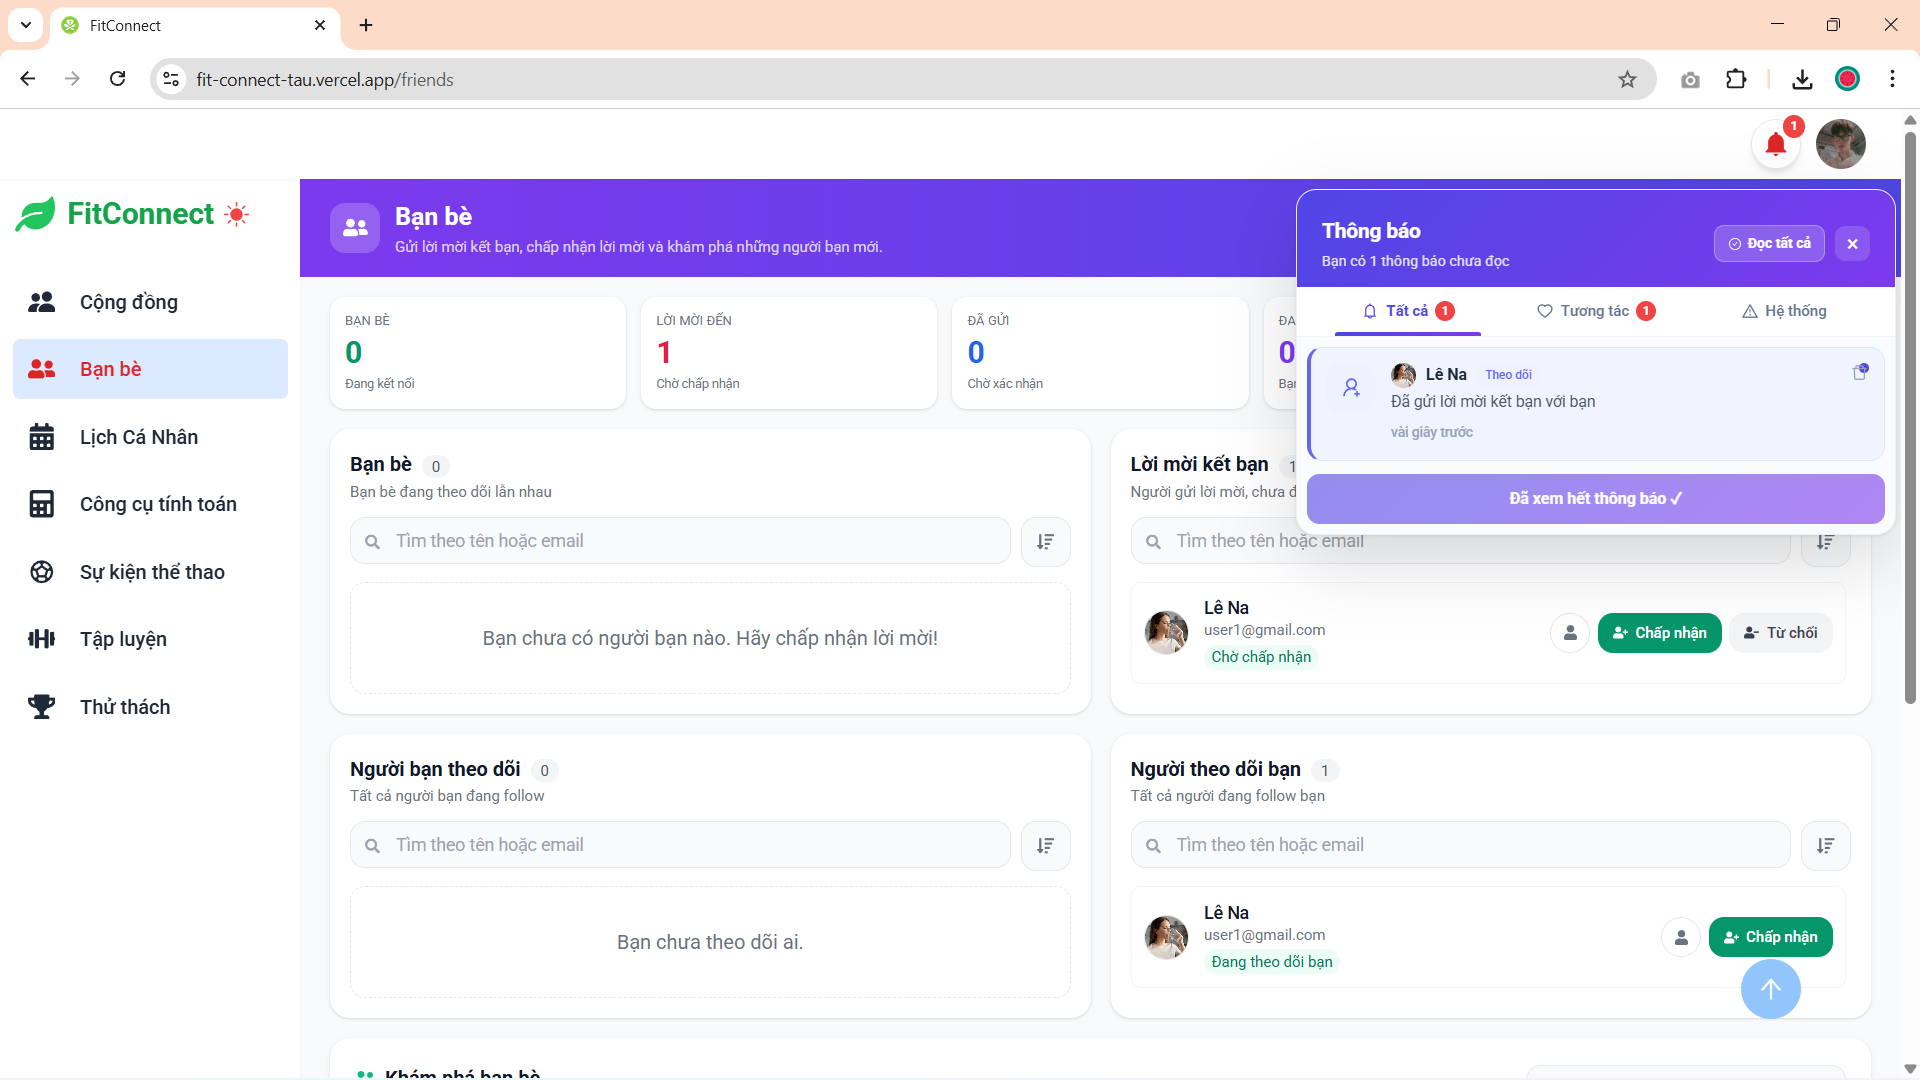
\includegraphics[width=0.60\textwidth]{Images/IMG/Nhom7/xemthongbaoguiketbanchominh.png}
    \caption{Người dùng nhận thông báo có lời mời kết bạn mới}
    \label{fig:impl_fr_request_noti}
\end{figure}


    \item Sau khi lời mời được chấp nhận, người gửi nhận thông báo xác nhận hai tài khoản đã trở thành bạn bè, đảm bảo cả hai bên đều nắm được trạng thái kết nối.

\end{itemize}

\subsubsection{Luồng thao tác mời bạn bè tham gia hoạt động}
\begin{itemize}
    \item Người dùng có thể mời bạn bè tham gia sự kiện thể thao hoặc thử thách cộng đồng ngay tại giao diện chi tiết. Hệ thống hiển thị modal chọn bạn bè để gửi lời mời nhanh theo danh sách kết nối hiện có.

\begin{figure}[H]
    \centering
    \begin{subfigure}[b]{0.45\textwidth}
        \centering
        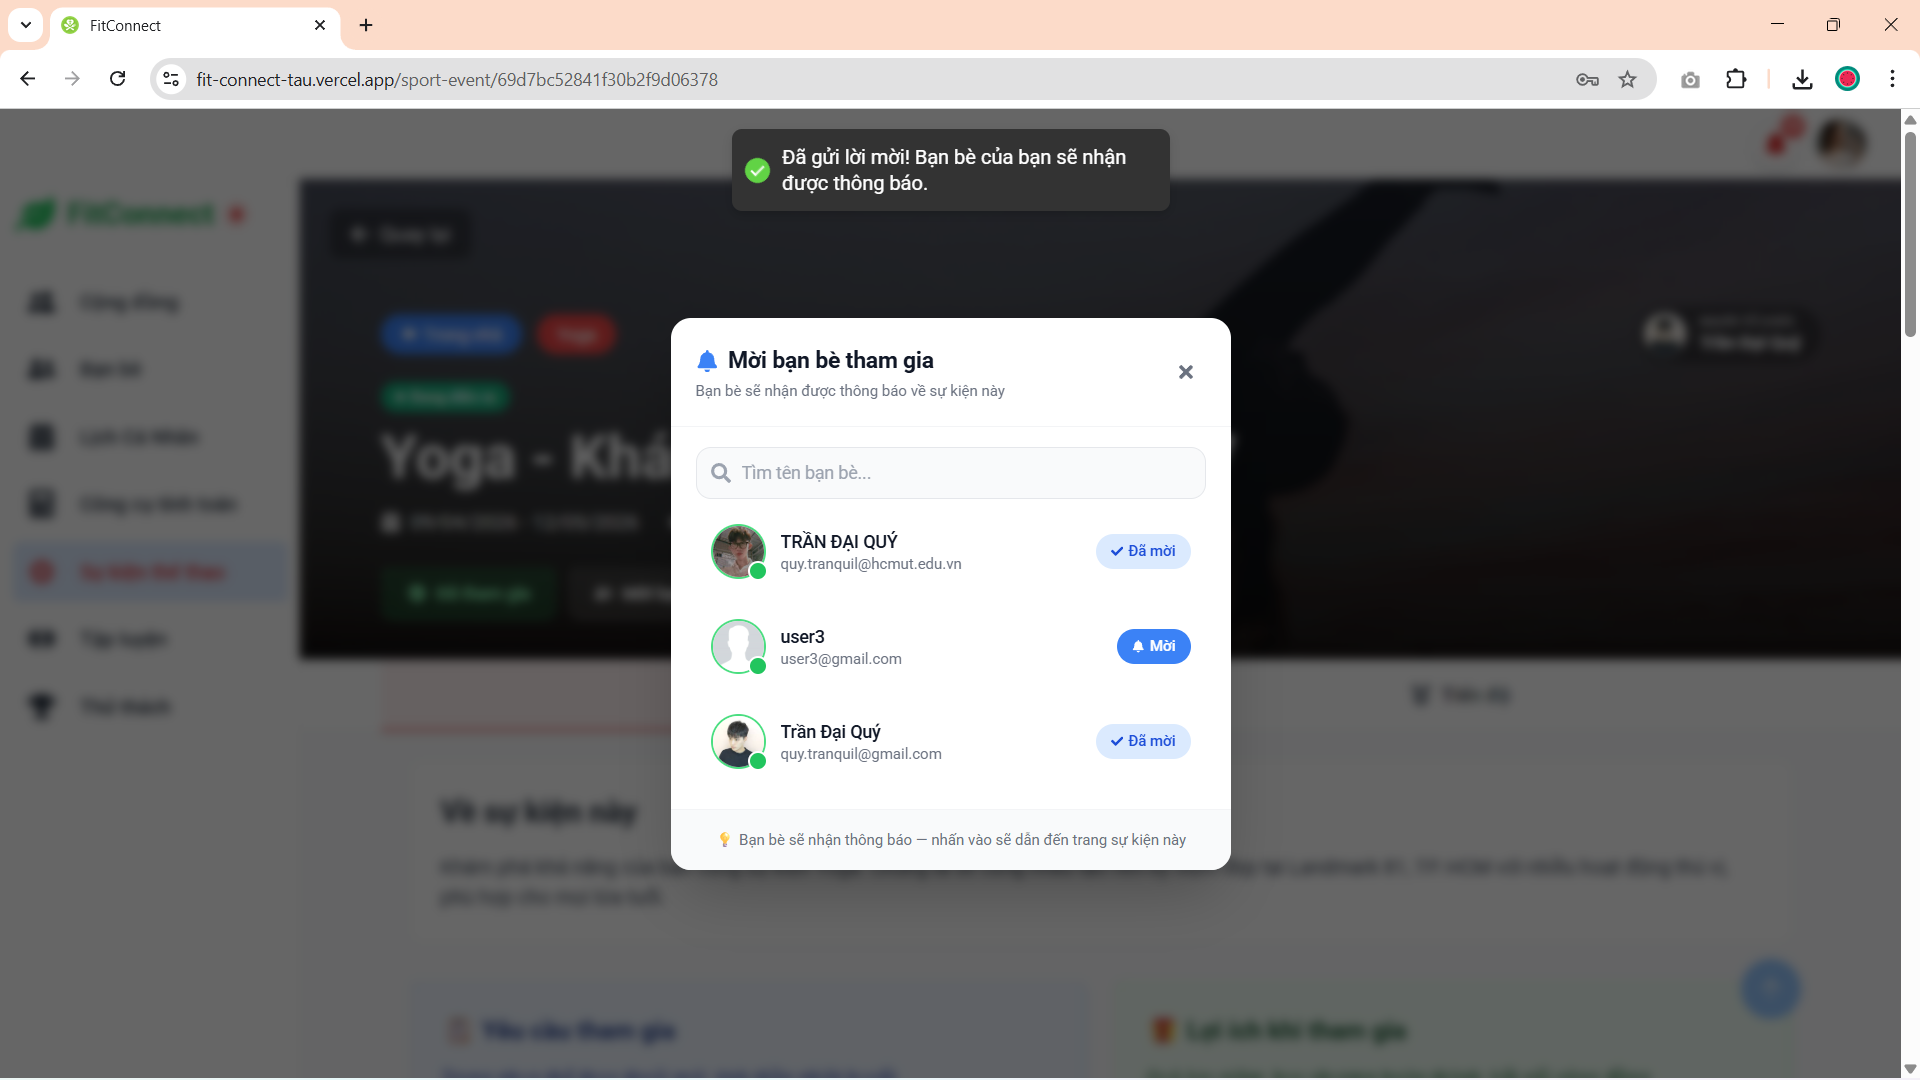
\includegraphics[width=\textwidth]{Images/IMG/Nhom7/moithamgiasukien.png}
        \caption{Mời bạn tham gia sự kiện}
        \label{fig:impl_fr_invite_event}
    \end{subfigure}
    \hfill
    \begin{subfigure}[b]{0.45\textwidth}
        \centering
        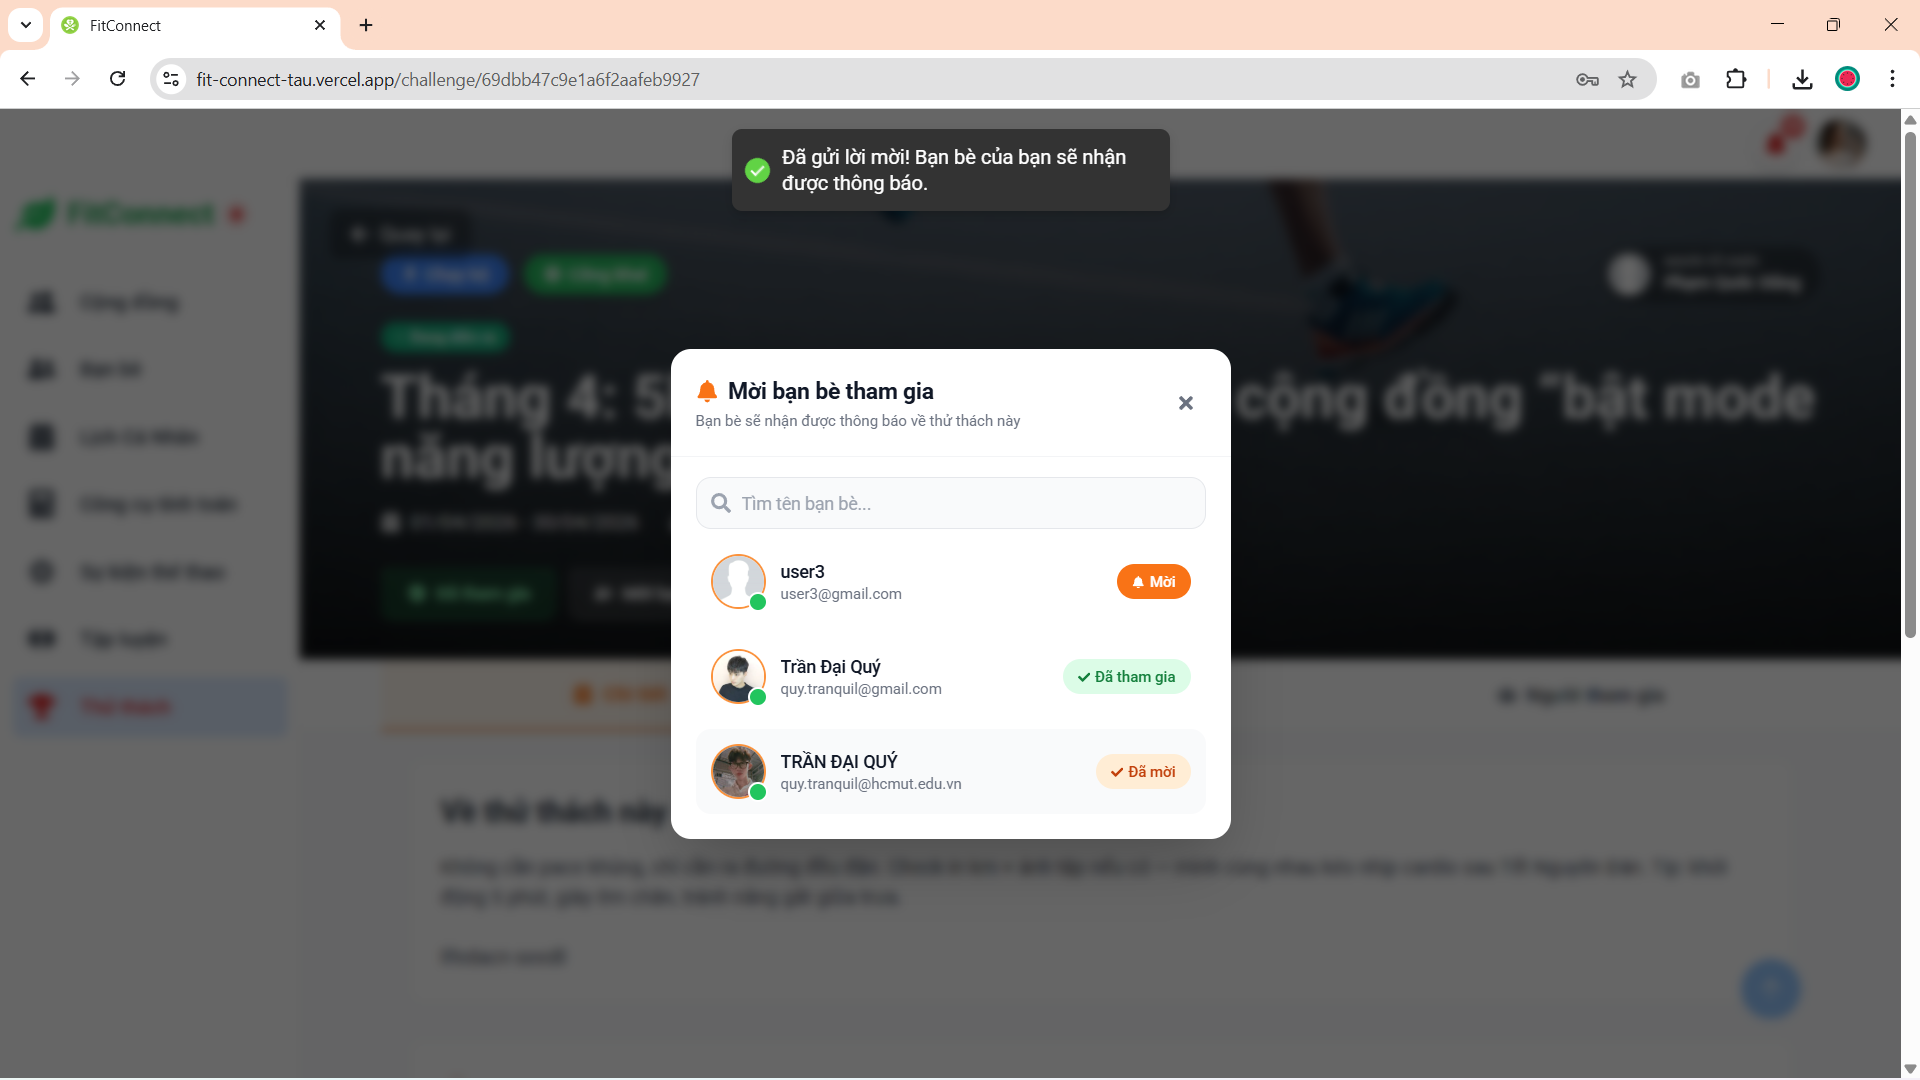
\includegraphics[width=\textwidth]{Images/IMG/Nhom7/moithamgiathuthach.png}
        \caption{Mời bạn tham gia thử thách}
        \label{fig:impl_fr_invite_challenge}
    \end{subfigure}
    \vspace{0.3em}
    \caption{Người dùng mời bạn bè tham gia hoạt động từ giao diện chi tiết}
    \label{fig:impl_fr_invite}
\end{figure}


    \item Khi được mời tham gia sự kiện hoặc thử thách, người dùng nhận thông báo lời mời trong hệ thống. Từ thông báo này, người dùng có thể truy cập nhanh nội dung được mời để xem chi tiết và quyết định tham gia.

\begin{figure}[H]
    \centering
    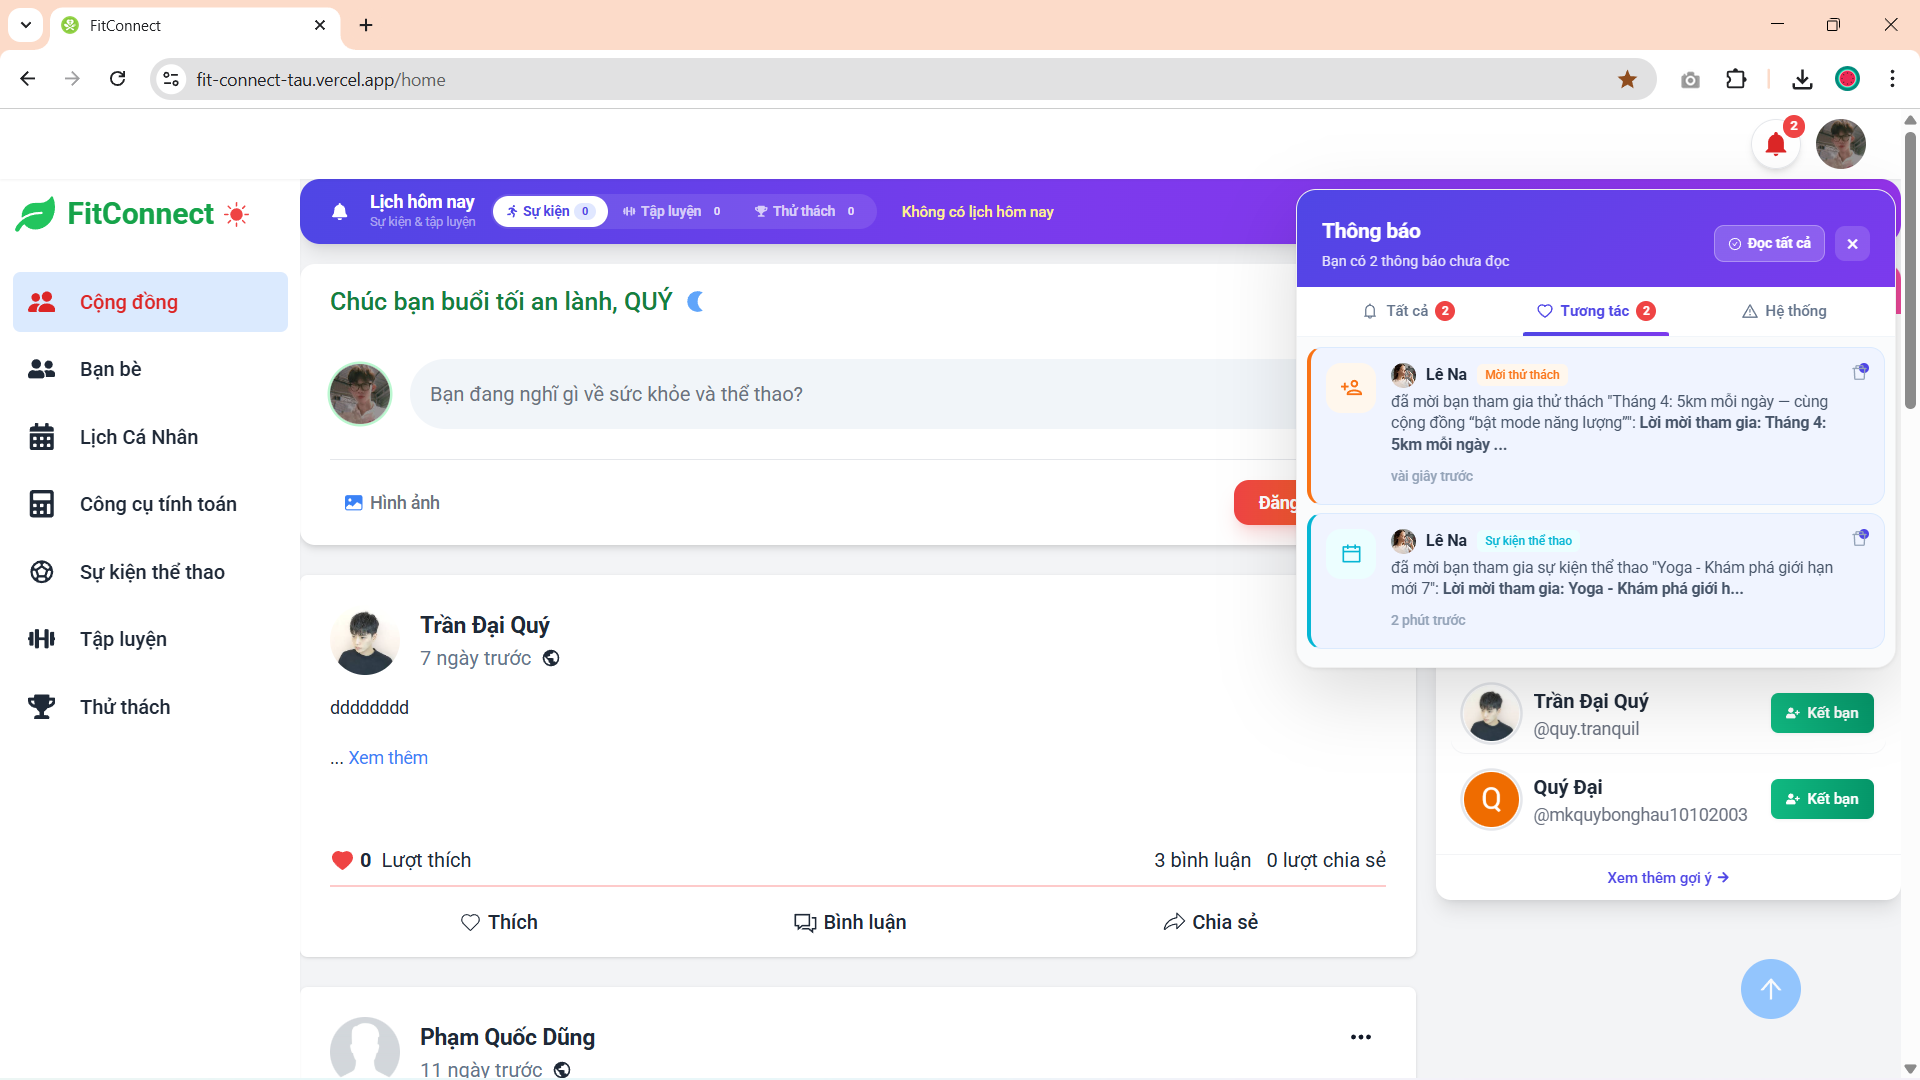
\includegraphics[width=0.60\textwidth]{Images/IMG/Nhom7/thongbaoloimoi.png}
    \caption{Hệ thống hiển thị thông báo lời mời tham gia hoạt động từ bạn bè}
    \label{fig:impl_fr_invite_noti}
\end{figure}

\end{itemize}

\subsection{Nhóm tính năng Quản trị hệ thống của Admin}
\label{subsec:impl_admin_system}

Nhóm tính năng Quản trị hệ thống là bộ công cụ dành riêng cho Quản trị viên (Admin) của nền tảng FitConnect, cung cấp khả năng giám sát toàn diện và điều hành tập trung các hoạt động trong hệ thống. Nhóm tính năng này bao gồm bốn trục nghiệp vụ cốt lõi: Giám sát Dashboard phân tích chuyên sâu, Quản trị người dùng và nhà kiểm duyệt, Kiểm duyệt nội dung đa tầng (bài viết, sự kiện, thử thách) và Quản lý hệ sinh thái dữ liệu (danh mục thể thao, thiết bị, kho bài tập). Giao diện Admin được xây dựng theo mô hình ``Hero-Stat'': mỗi trang quản lý gồm banner gradient chủ đề, thẻ thống kê tóm tắt và bảng dữ liệu mật độ cao nhằm tối ưu hóa trải nghiệm điều hành.

\subsubsection{Luồng thao tác giám sát tổng quan Dashboard}
\begin{itemize}
    \item Quản trị viên truy cập trang Dashboard, hệ thống hiển thị toàn cảnh bức tranh hoạt động thông qua các khối phân tích chuyên sâu. Tại phần \textbf{Tổng quan Hệ thống}, hệ thống cung cấp các thẻ số liệu cốt lõi (tài khoản, sự kiện, thử thách) với thiết kế trực quan giúp Admin nhanh chóng nắm bắt quy mô hiện tại của nền tảng.

\begin{figure}[H]
    \centering
    
\includegraphics[width=0.60\textwidth]{Images/IMG/nhom9/dashboard/dashboard.png}
    \caption{Trang Dashboard Tổng quan của Quản trị viên -- Toàn cảnh hệ thống}
    \label{fig:impl_admin_dashboard_overview}
\end{figure}


    \item Tại khối \textbf{Người dùng \& Sức khỏe}, hệ thống tự động phân tích và biểu đồ hóa dữ liệu nhân khẩu học (giới tính), mức độ tham gia hoạt động và phân bố chỉ số BMI của cộng đồng. Đồng thời, hệ thống còn vinh danh các cá nhân tích cực thông qua danh sách người dùng nổi bật.

    \item Đối với khối \textbf{Cộng đồng \& Sự kiện}, hệ thống theo dõi mức độ tăng trưởng thông qua biểu đồ xu hướng theo thời gian, giúp nhận diện sự kiện nào đang thu hút sự chú ý (phân loại sự kiện ngoài trời, trong nhà) và các môn thể thao phổ biến nhất trong cộng đồng.

    \item Tại khối \textbf{Thử thách}, Quản trị viên có thể giám sát hệ sinh thái thử thách thông qua các biểu đồ phân tích cơ cấu loại thử thách và phạm vi tham gia, từ đó có cái nhìn chi tiết về xu hướng rèn luyện sức khỏe của người dùng.
\end{itemize}

\subsubsection{Luồng thao tác quản lý người dùng}
\begin{itemize}
    \item Tại trang quản lý người dùng, hệ thống cung cấp một danh sách tổng hợp tất cả tài khoản với đầy đủ thông tin định danh và lịch sử vi phạm. Quản trị viên có thể sử dụng các công cụ tìm kiếm và sắp xếp để nhanh chóng truy xuất thông tin của bất kỳ người dùng nào trên hệ thống.

\begin{figure}[H]
    \centering
    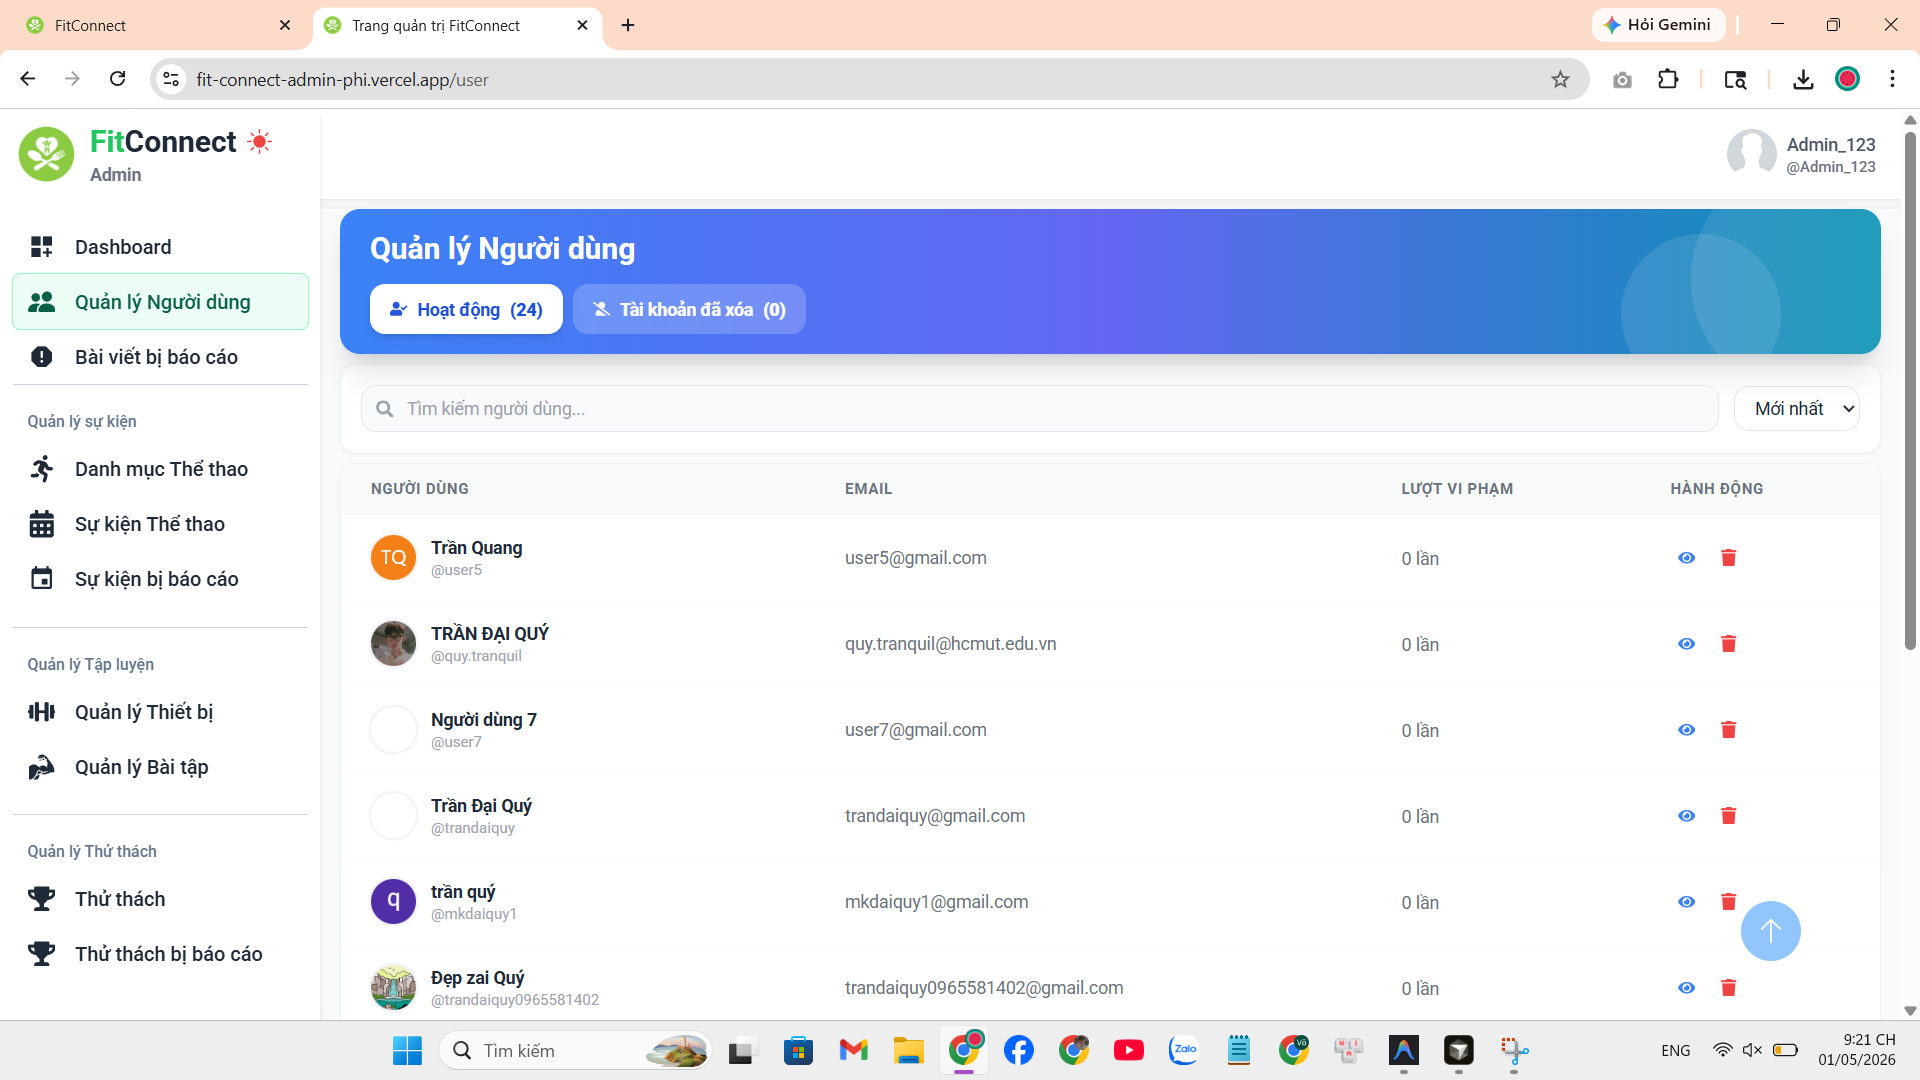
\includegraphics[width=0.60\textwidth]{Images/IMG/nhom9/quanlynguoidung/danhsachnguoidung.png}
    \caption{Quản trị viên xem danh sách người dùng đang hoạt động}
    \label{fig:impl_admin_user_list}
\end{figure}


    \item Để đánh giá mức độ tương tác, Admin có thể xem chi tiết hồ sơ hoạt động của từng cá nhân. Hệ thống sẽ mở ra một panel hiển thị chi tiết số liệu đóng góp của người đó trong cộng đồng cũng như tần suất tham gia sự kiện, thử thách.

\begin{figure}[H]
    \centering
    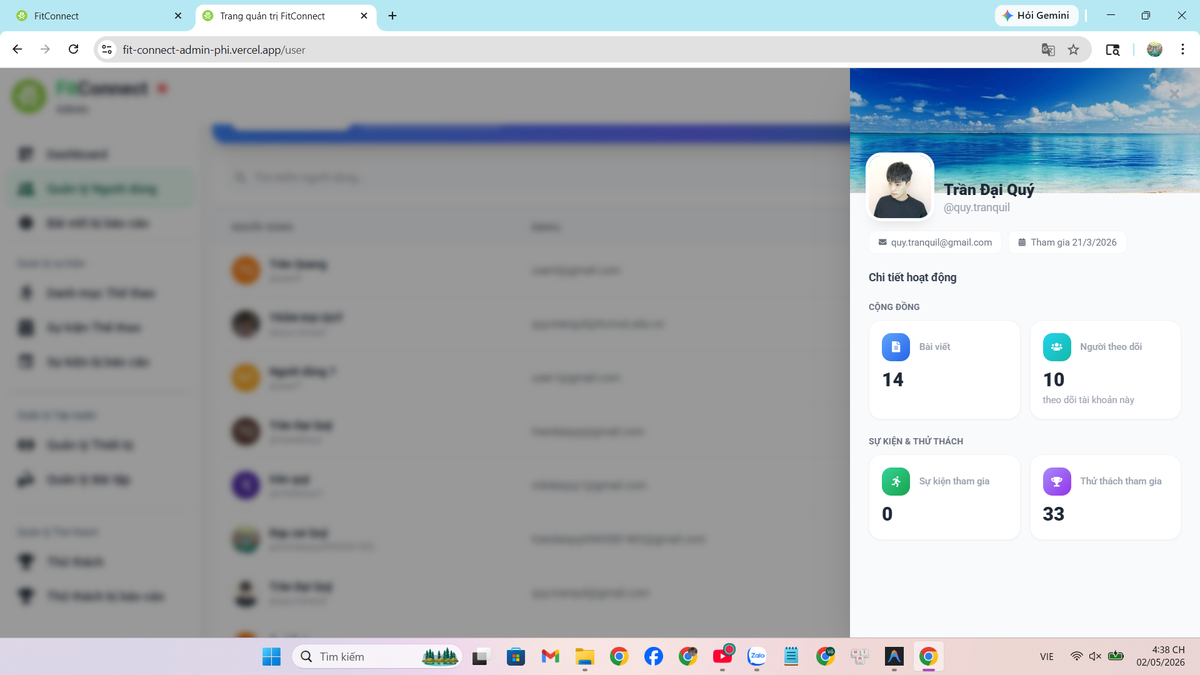
\includegraphics[width=0.60\textwidth]{Images/IMG/nhom9/quanlynguoidung/chitietnguoidung.png}
    \caption{Quản trị viên xem chi tiết hoạt động của người dùng}
    \label{fig:impl_admin_user_detail}
\end{figure}


    \item Khi phát hiện vi phạm, hệ thống hỗ trợ thao tác khóa tài khoản thông qua cơ chế xóa mềm (soft delete). Thao tác này yêu cầu xác nhận hai bước nhằm tránh rủi ro thao tác nhầm, đồng thời bảo toàn tính nguyên vẹn của dữ liệu lịch sử để phục vụ tra cứu sau này.

\begin{figure}[H]
    \centering
    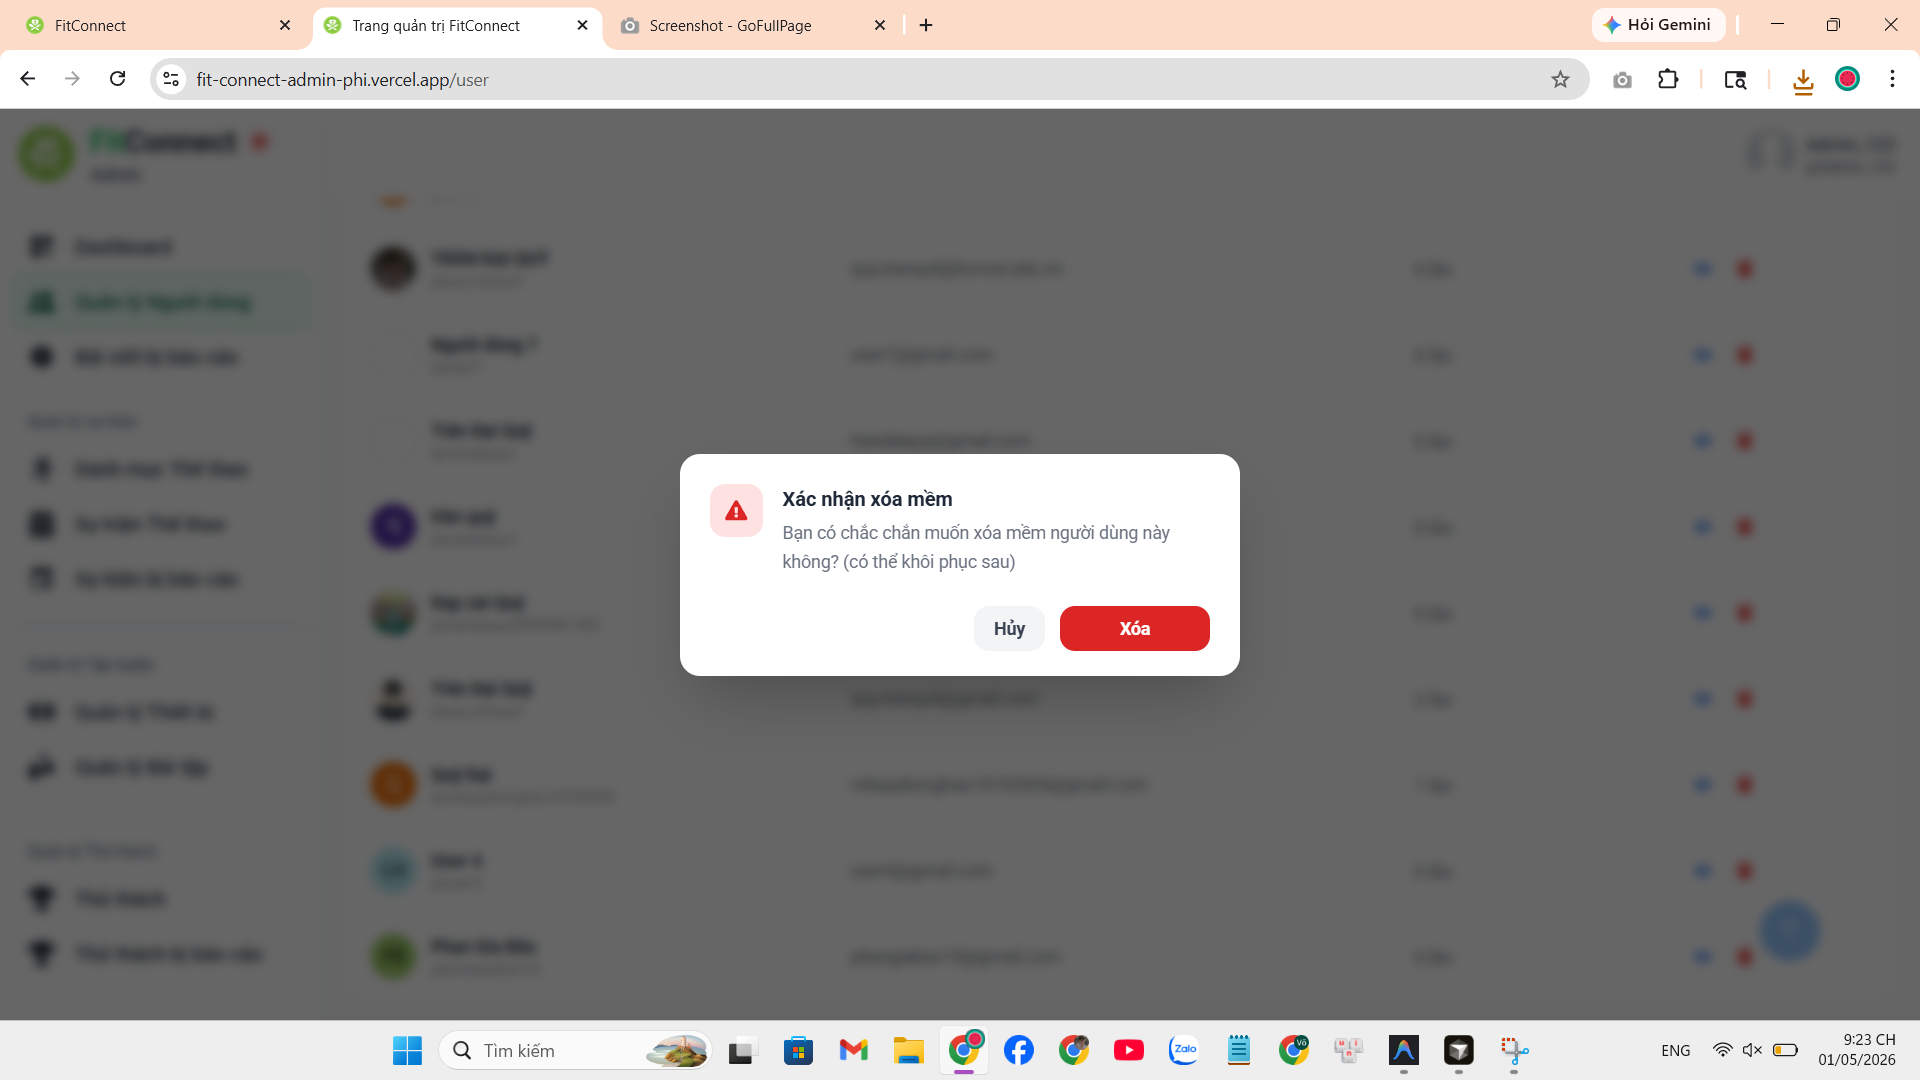
\includegraphics[width=0.60\textwidth]{Images/IMG/nhom9/quanlynguoidung/xoanguoidung.png}
    \caption{Hệ thống hiển thị hộp thoại xác nhận khóa tài khoản người dùng}
    \label{fig:impl_admin_user_delete_confirm}
\end{figure}


    \item Tài khoản vi phạm bị chuyển vào danh sách ``Đã xóa''; người dùng nhận thông báo lỗi xác thực khi đăng nhập. Hệ thống cho phép khôi phục tài khoản nếu xử lý sai lệch hoặc người dùng đã khắc phục vi phạm.

\begin{figure}[H]
    \centering
    \begin{subfigure}[b]{0.47\textwidth}
        \centering
        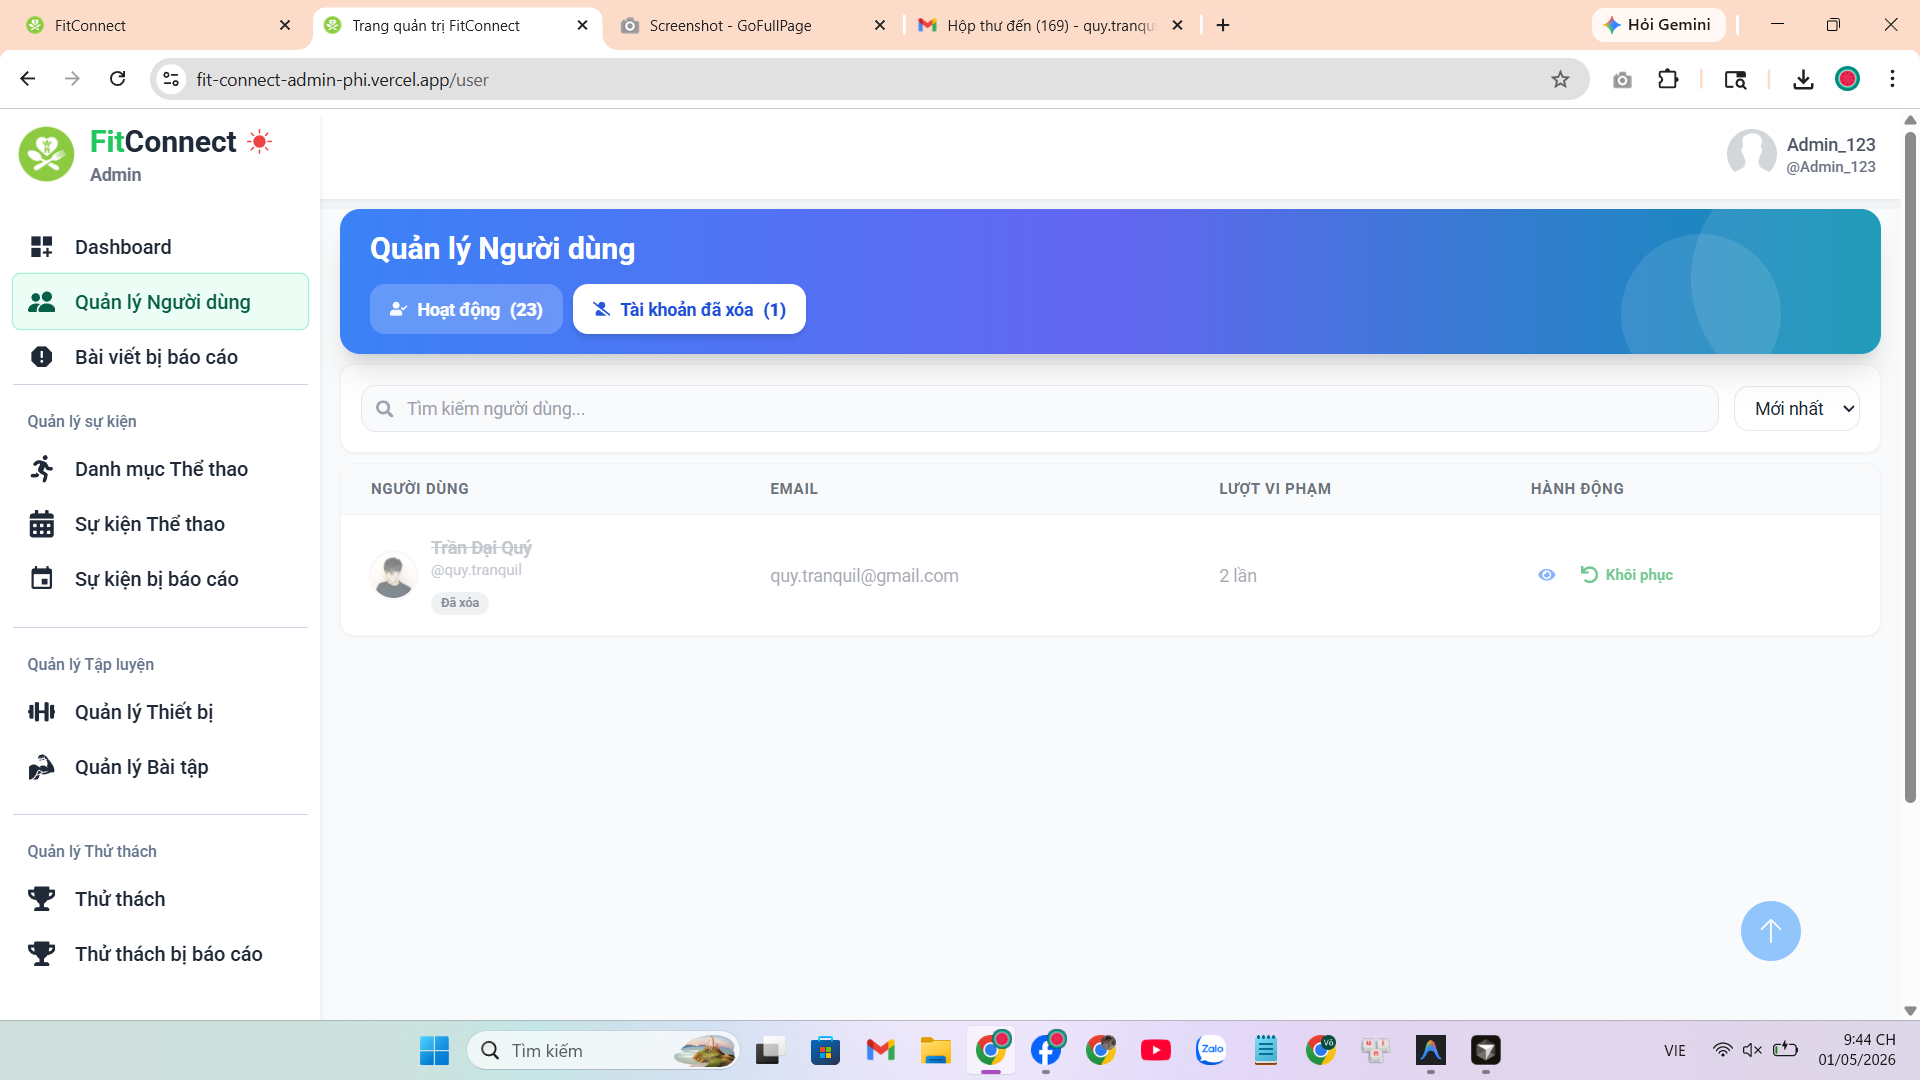
\includegraphics[width=\textwidth]{Images/IMG/nhom9/quanlynguoidung/nguoidungbixoa.png}
        \caption{Danh sách tài khoản đã bị vô hiệu hóa}
        \label{fig:impl_admin_user_deleted_list}
    \end{subfigure}
    \hfill
    \begin{subfigure}[b]{0.47\textwidth}
        \centering
        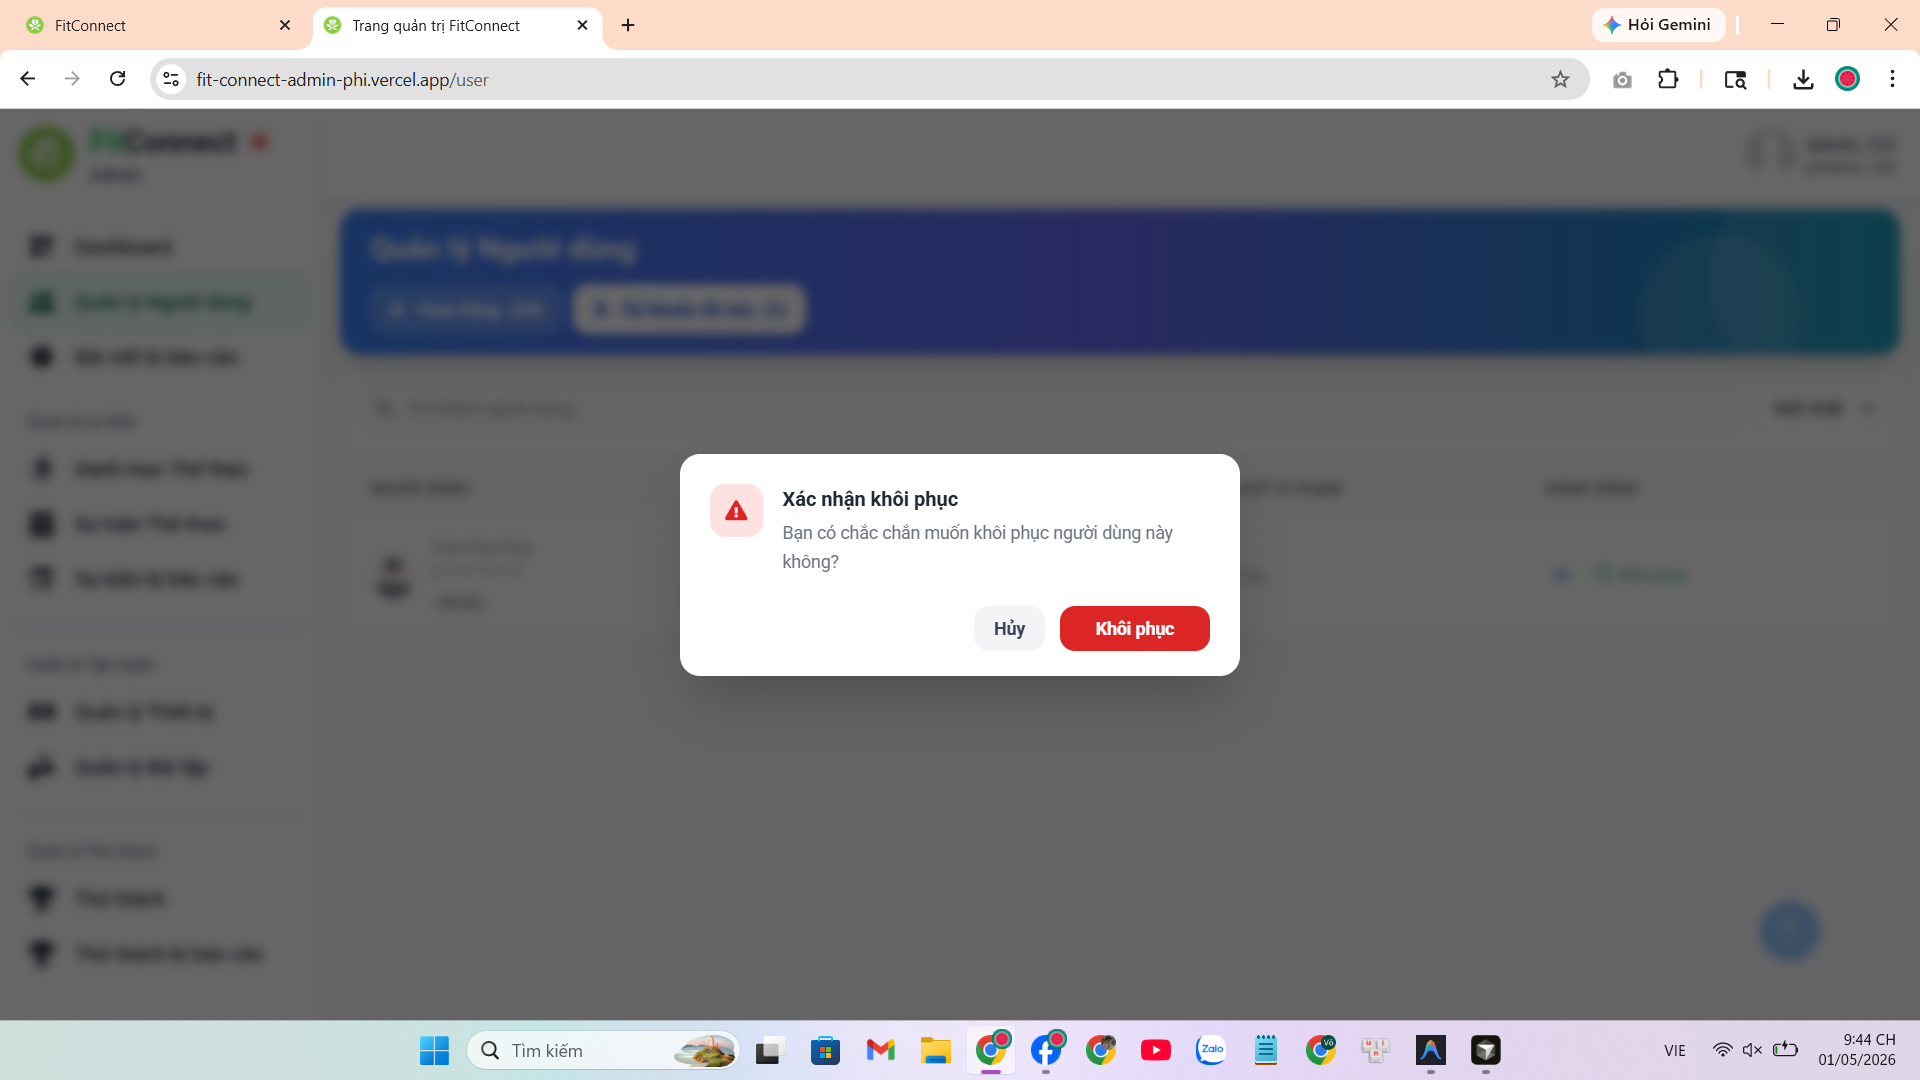
\includegraphics[width=\textwidth]{Images/IMG/nhom9/quanlynguoidung/modalkhoiphucnguoidungbixoa.png}
        \caption{Xác nhận khôi phục tài khoản người dùng}
        \label{fig:impl_admin_user_restore_confirm}
    \end{subfigure}
    \vspace{0.3em}
    \caption{Quản lý tài khoản bị vô hiệu hóa và quy trình khôi phục}
    \label{fig:impl_admin_user_ban_restore}
\end{figure}

\end{itemize}

\subsubsection{Luồng thao tác kiểm duyệt bài viết}
\begin{itemize}
    \item Quy trình kiểm duyệt bắt nguồn từ các báo cáo vi phạm của cộng đồng. Người dùng thao tác báo cáo nội dung không phù hợp trực tiếp trên bảng tin bài viết.

\begin{figure}[H]
    \centering
    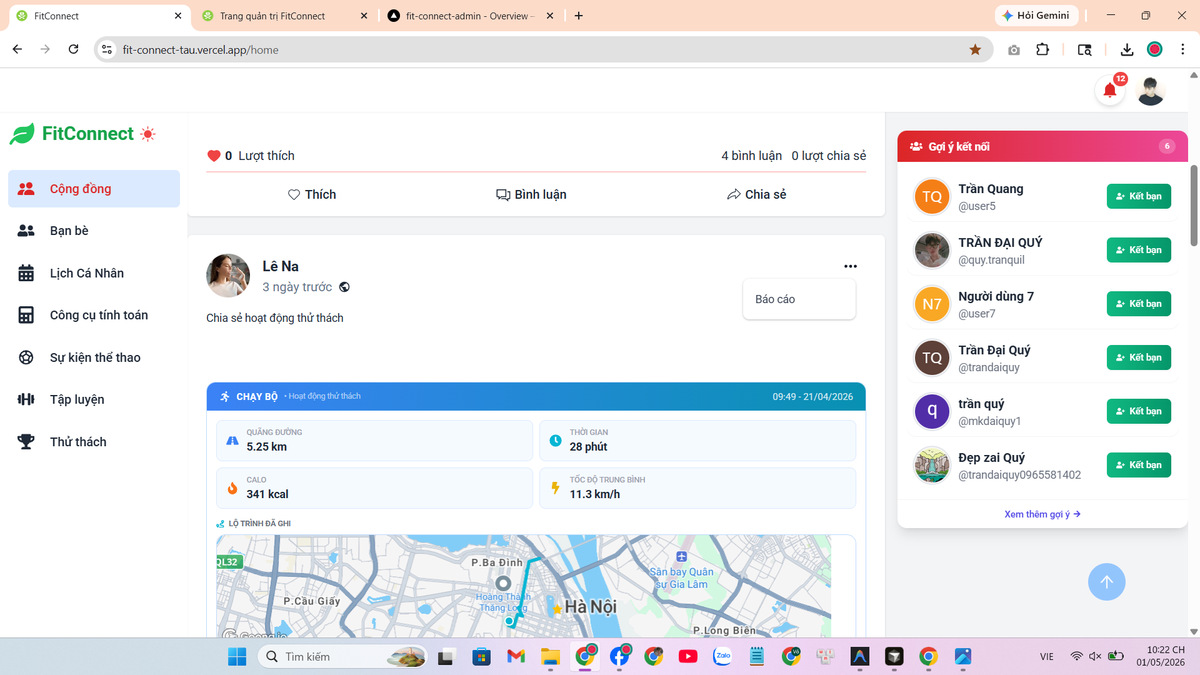
\includegraphics[width=0.60\textwidth]{Images/IMG/nhom9/quanlybaiviet/baocaobaiviet.png}
    \caption{Người dùng thực hiện báo cáo bài viết vi phạm trên trang Cộng đồng}
    \label{fig:impl_admin_post_report_action}
\end{figure}


    \item Tại trang kiểm duyệt, hệ thống tập hợp toàn bộ các báo cáo chờ xử lý. Quản trị viên có thể theo dõi danh sách các bài viết bị gắn cờ, kèm theo thông tin chi tiết về số lượng báo cáo và đánh giá mức độ nghiêm trọng.

\begin{figure}[H]
    \centering
    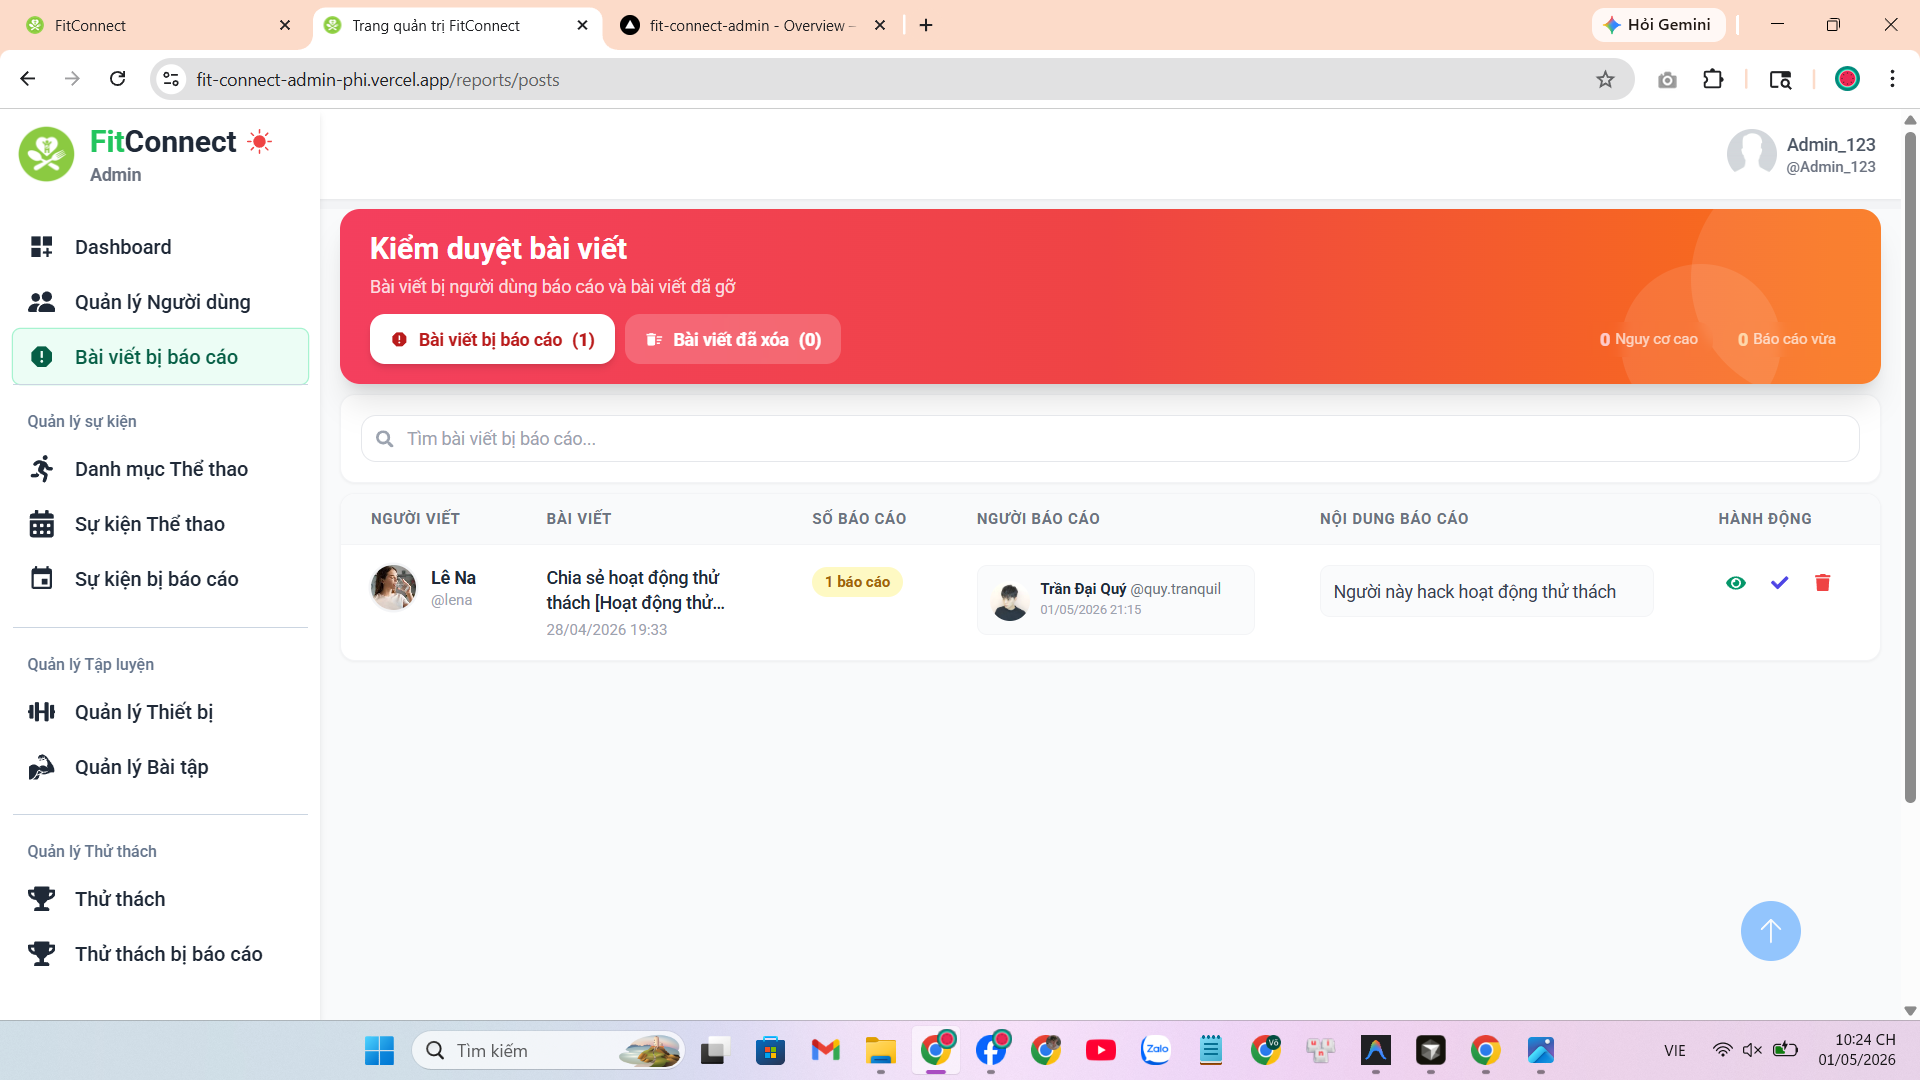
\includegraphics[width=0.60\textwidth]{Images/IMG/nhom9/quanlybaiviet/baivietbibaocao.png}
    \caption{Quản trị viên xem danh sách bài viết bị người dùng báo cáo}
    \label{fig:impl_admin_post_reported_list}
\end{figure}


    \item Để đảm bảo tính công bằng, hệ thống cung cấp giao diện hiển thị trọn vẹn nội dung bài viết gốc cùng danh sách lý do báo cáo, hỗ trợ Admin xem xét toàn diện trước khi đưa ra quyết định xử lý.

\begin{figure}[H]
    \centering
    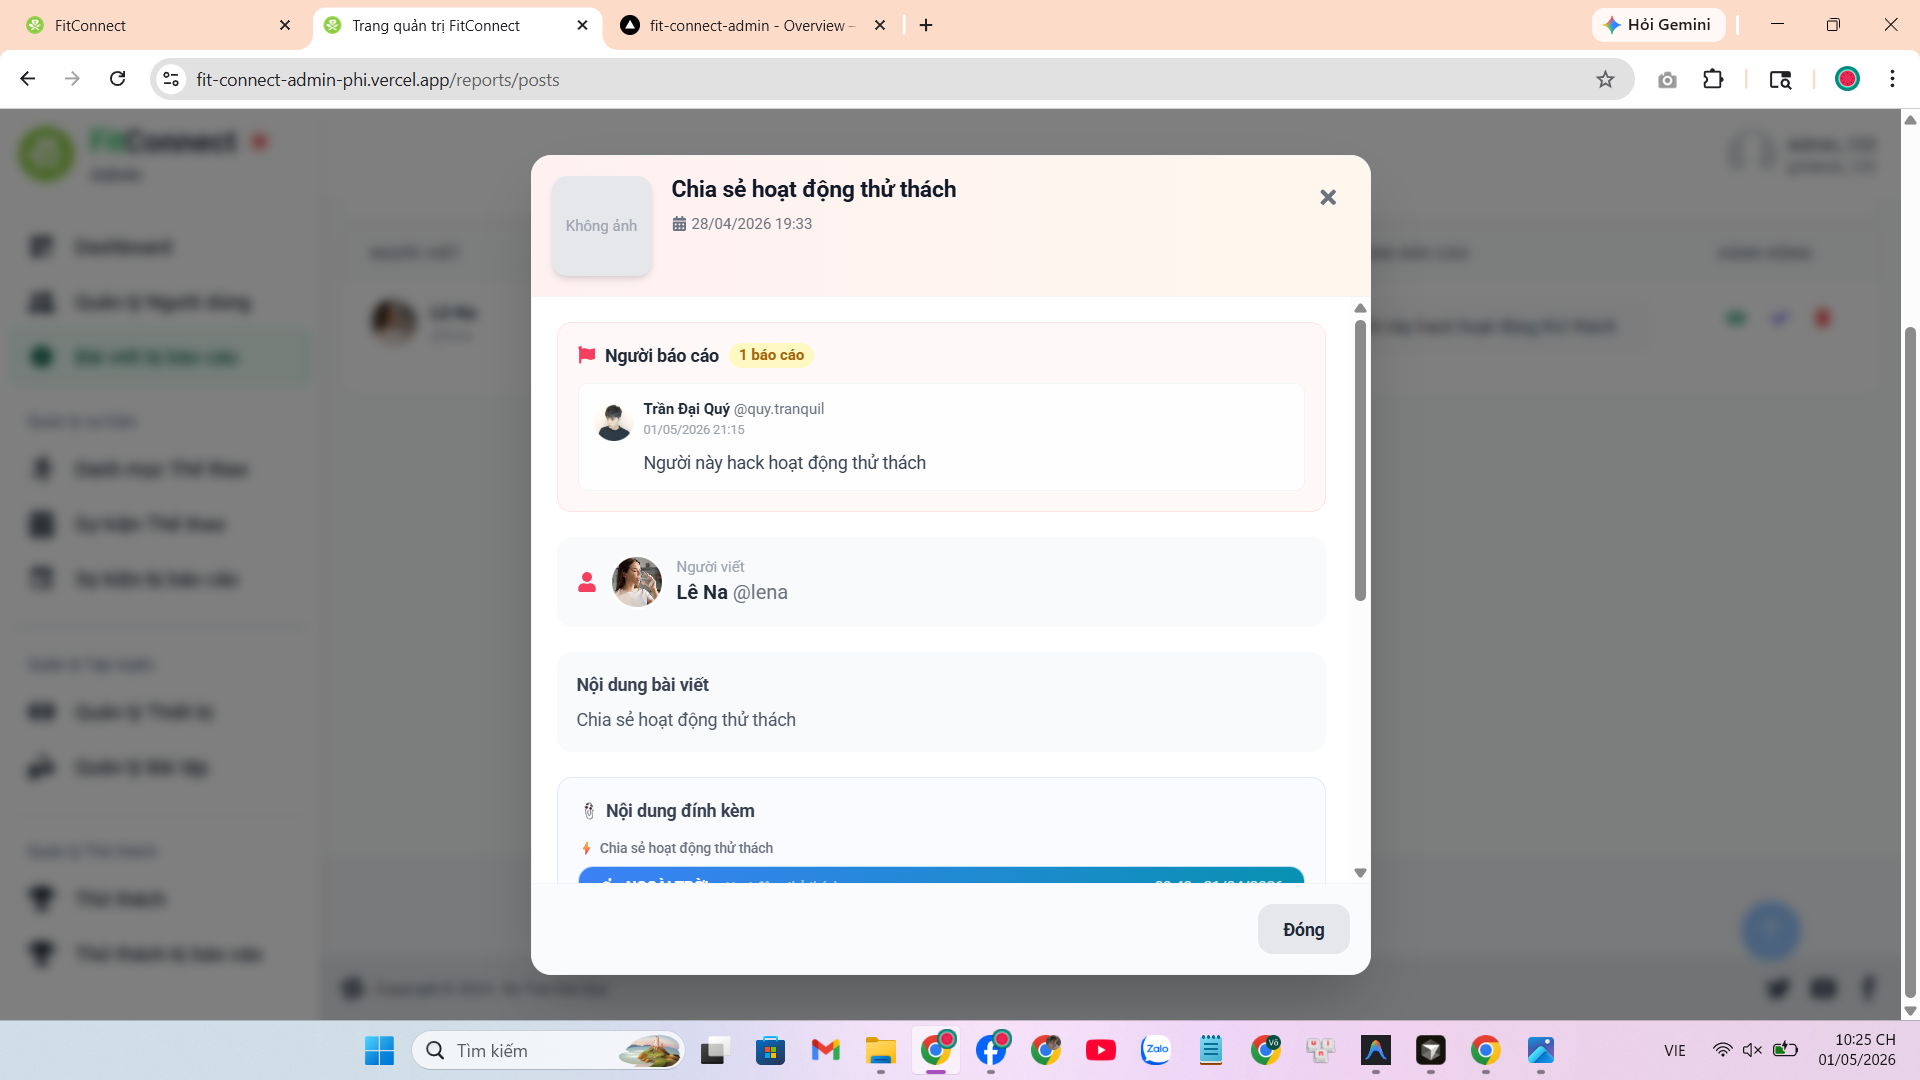
\includegraphics[width=0.60\textwidth]{Images/IMG/nhom9/quanlybaiviet/xemduocnoidungbaivietbibaocao.png}
    \caption{Quản trị viên xem chi tiết nội dung bài viết bị báo cáo kèm thông tin người báo cáo}
    \label{fig:impl_admin_post_report_detail}
\end{figure}


    \item Dựa trên phân tích, Admin \textbf{Gỡ bỏ} bài viết vi phạm (ẩn ngay khỏi bảng tin) hoặc \textbf{Giữ lại} nếu báo cáo không hợp lệ. Bài viết đã gỡ vào kho ``Đã xóa'' và có thể khôi phục trở lại bảng tin bất kỳ lúc nào.

\begin{figure}[H]
    \centering
    \begin{subfigure}[b]{0.47\textwidth}
        \centering
        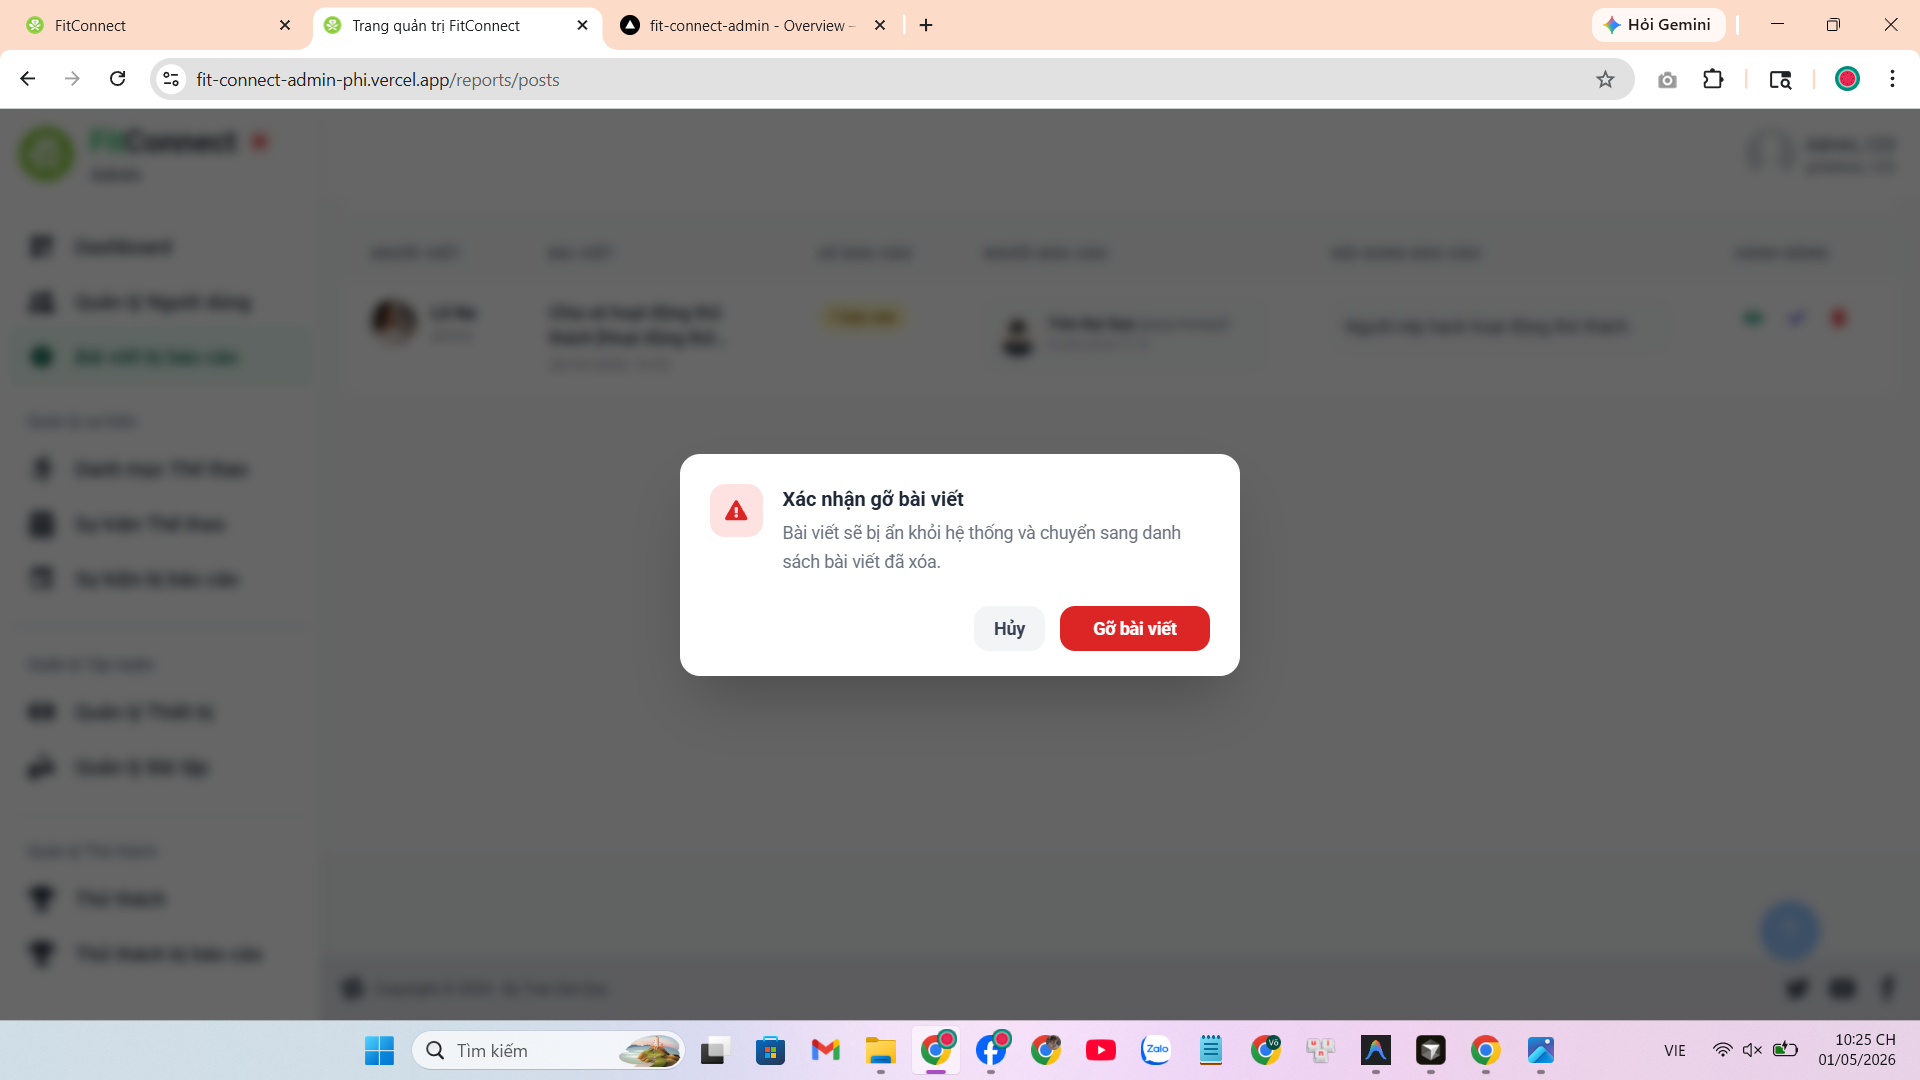
\includegraphics[width=\textwidth]{Images/IMG/nhom9/quanlybaiviet/xacnhanxoabaiviet.png}
        \caption{Xác nhận gỡ bài viết vi phạm}
        \label{fig:impl_admin_post_delete_confirm}
    \end{subfigure}
    \hfill
    \begin{subfigure}[b]{0.47\textwidth}
        \centering
        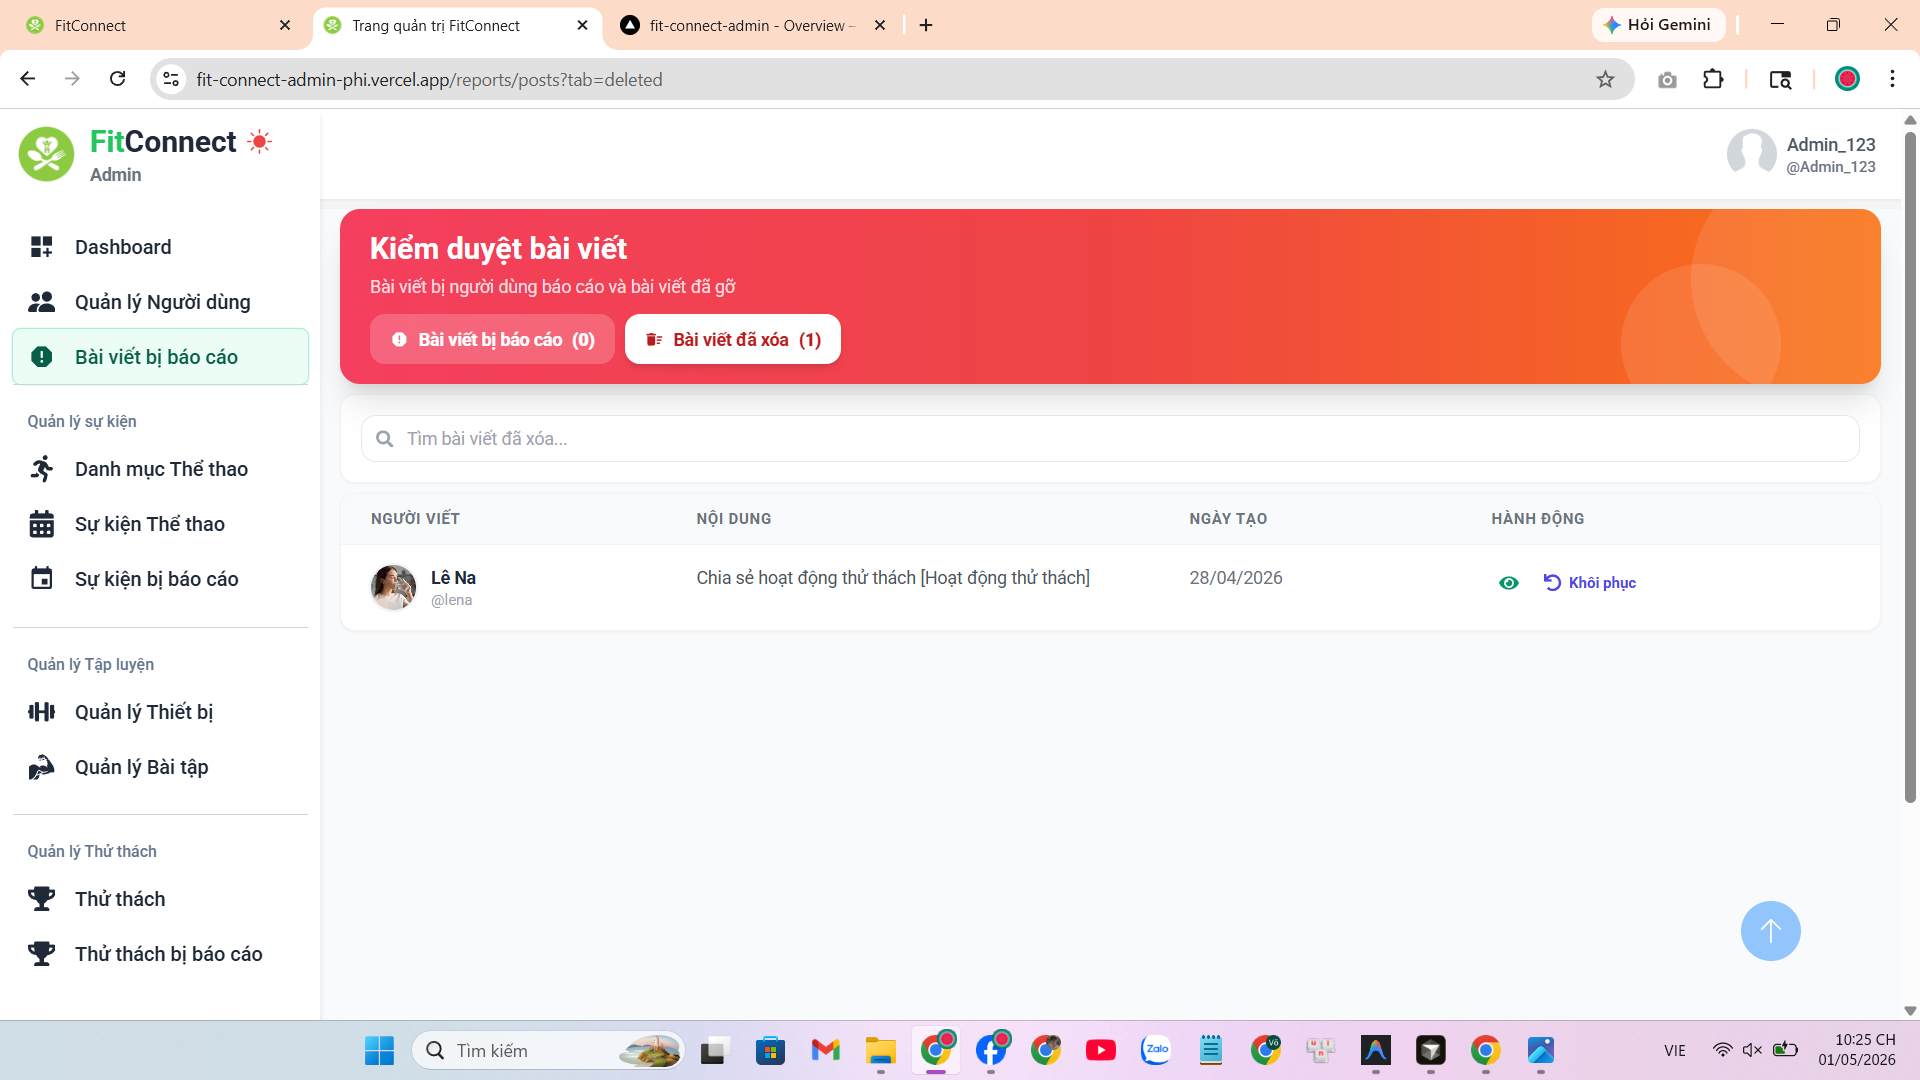
\includegraphics[width=\textwidth]{Images/IMG/nhom9/quanlybaiviet/danhsachbaivietbixoa.png}
        \caption{Danh sách bài viết đã gỡ và tùy chọn khôi phục}
        \label{fig:impl_admin_post_deleted_list}
    \end{subfigure}
    \vspace{0.3em}
    \caption{Xử lý bài viết vi phạm và quản lý kho lưu trữ bài viết đã gỡ}
    \label{fig:impl_admin_post_moderation}
\end{figure}

\end{itemize}

\subsubsection{Luồng thao tác quản lý danh mục thể thao}

\textbf{Cơ sở tính toán định mức Kcal:}

Để đảm bảo tính khoa học và nhất quán trên toàn nền tảng, hệ số tiêu thụ calo (Kcal) của từng môn thể thao được xây dựng dựa trên \textbf{Chỉ số chuyển hóa cơ bản (MET - Metabolic Equivalent of Task)}, tham chiếu trực tiếp từ cơ sở dữ liệu chuẩn quốc tế Compendium of Physical Activities \cite{CompendiumPhysicalActivities}. Hệ thống thực hiện chuẩn hóa số liệu bằng cách tính toán Kcal tiêu thụ trung bình dựa trên giả định cân nặng người dùng từ 65kg đến 70kg, nhằm tối ưu hóa hiệu suất xử lý hệ thống mà không yêu cầu cá nhân hóa theo từng người dùng.

Công thức tính toán gốc được áp dụng như sau:
\begin{itemize}
    \item Đối với hoạt động đo theo thời gian (phút): $\text{Kcal/phút} = \frac{\text{MET} \times 3.5 \times \text{Cân nặng (kg)}}{200}$
    \item Đối với hoạt động đo theo khoảng cách (km): $\text{Kcal/km} = \text{Kcal/phút} \times \text{Thời gian trung bình (phút) / km}$
\end{itemize}

Từ đó, hệ thống cấu hình tham số Kcal/Đơn vị và áp dụng vào hai luồng đo lường chính:
\begin{itemize}
    \item \textbf{Thể thao trong nhà (Tương tác qua Video Call):} $\text{Lượng Kcal} = \frac{\text{Thời gian hoạt động (giây)}}{60} \times \text{Kcal/phút}$. Trường hợp môn thể thao chưa được cập nhật hệ số, hệ thống sẽ sử dụng giá trị mặc định là $4\text{ Kcal/phút}$.
    \item \textbf{Thể thao ngoài trời (Theo dõi GPS):} $\text{Lượng Kcal} = \text{Khoảng cách (km)} \times \text{Kcal/km}$.
\end{itemize}

\textbf{Luồng thao tác quản trị trên hệ thống:}
\begin{itemize}
    \item Trang quản lý Danh mục Thể thao đóng vai trò là nơi cấu hình dữ liệu gốc cho toàn bộ các hoạt động thể chất trên nền tảng. Khi truy cập, Quản trị viên được cung cấp danh sách đầy đủ các môn thể thao đang được hỗ trợ, phân loại theo nhóm ``Ngoài trời'' và ``Trong nhà''. Mỗi danh mục hiển thị thông tin trực quan về tên môn, loại hình và định mức tiêu thụ calo (Kcal/Đơn vị) như đã trình bày ở trên.

\begin{figure}[H]
    \centering
    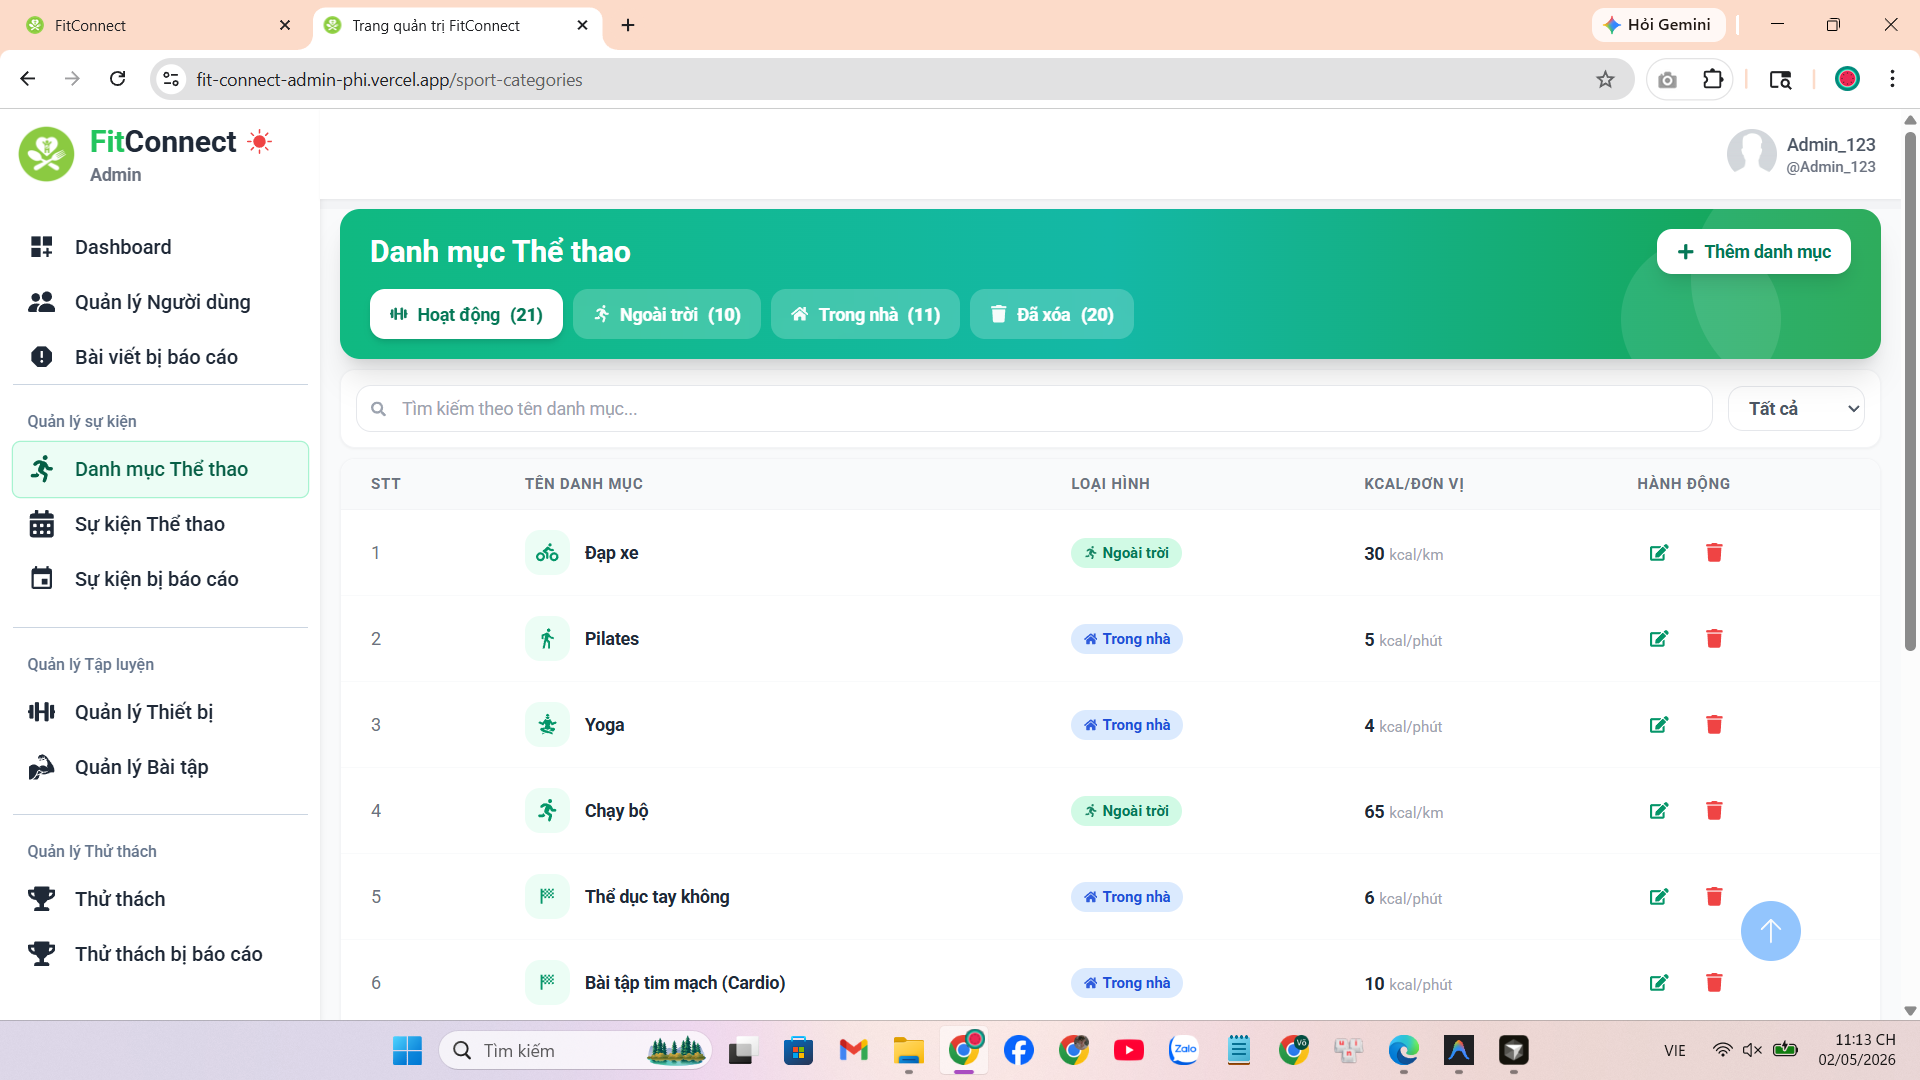
\includegraphics[width=0.60\textwidth]{Images/IMG/nhom9/danhmucthethao/danhsachdanhmucthethao.png}
    \caption{Quản trị viên xem danh sách các danh mục thể thao đang hoạt động}
    \label{fig:impl_admin_category_list}
\end{figure}


    \item Quản trị viên có thẩm quyền cập nhật các thông số của danh mục, đặc biệt là hệ số tiêu thụ Kcal. Khi thực hiện thay đổi trên hệ thống quản trị, giá trị này sẽ trở thành cơ sở tính toán mới cho toàn bộ các sự kiện và thử thách liên quan trên ứng dụng của người dùng.

\begin{figure}[H]
    \centering
    \begin{subfigure}[b]{0.47\textwidth}
        \centering
        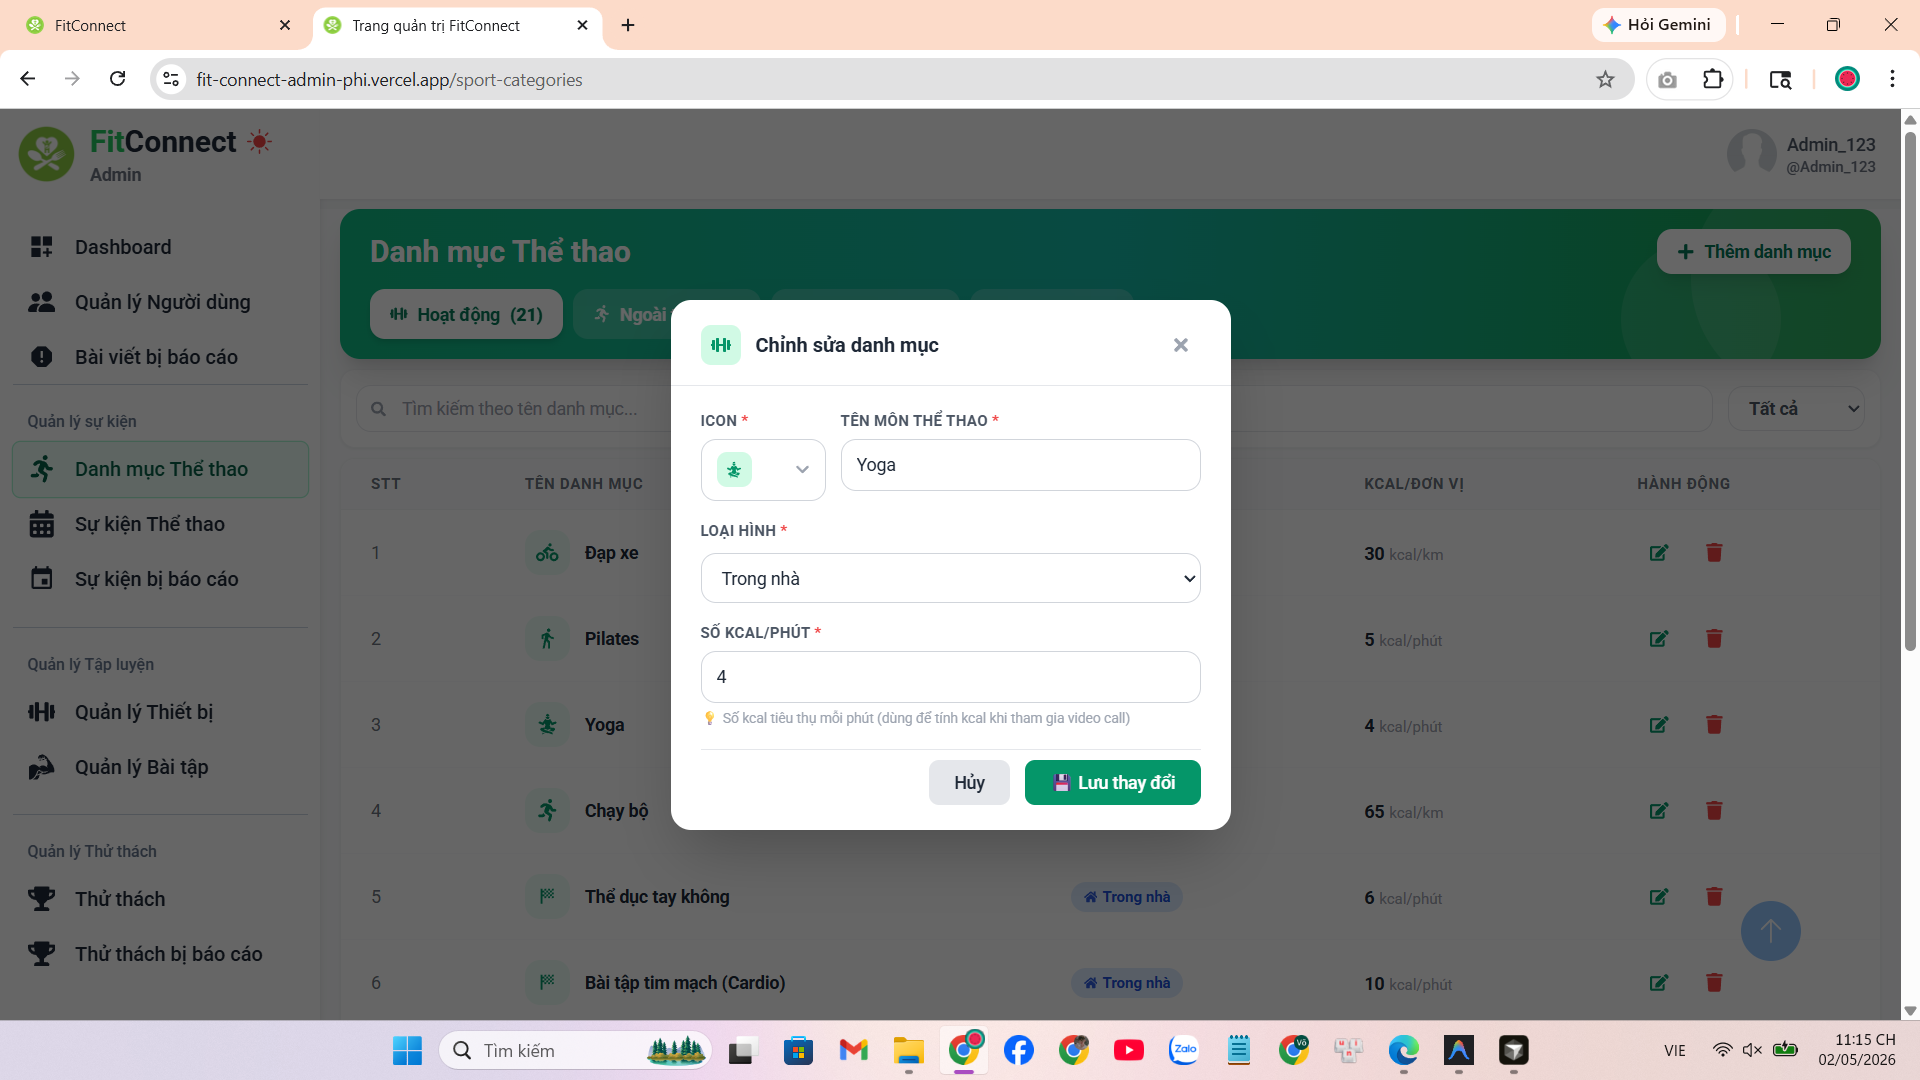
\includegraphics[width=\textwidth]{Images/IMG/nhom9/danhmucthethao/modalchinhsuadanhmuc.png}
        \caption{Hộp thoại chỉnh sửa thông tin danh mục}
        \label{fig:impl_admin_category_edit_modal}
    \end{subfigure}
    \hfill
    \begin{subfigure}[b]{0.47\textwidth}
        \centering
        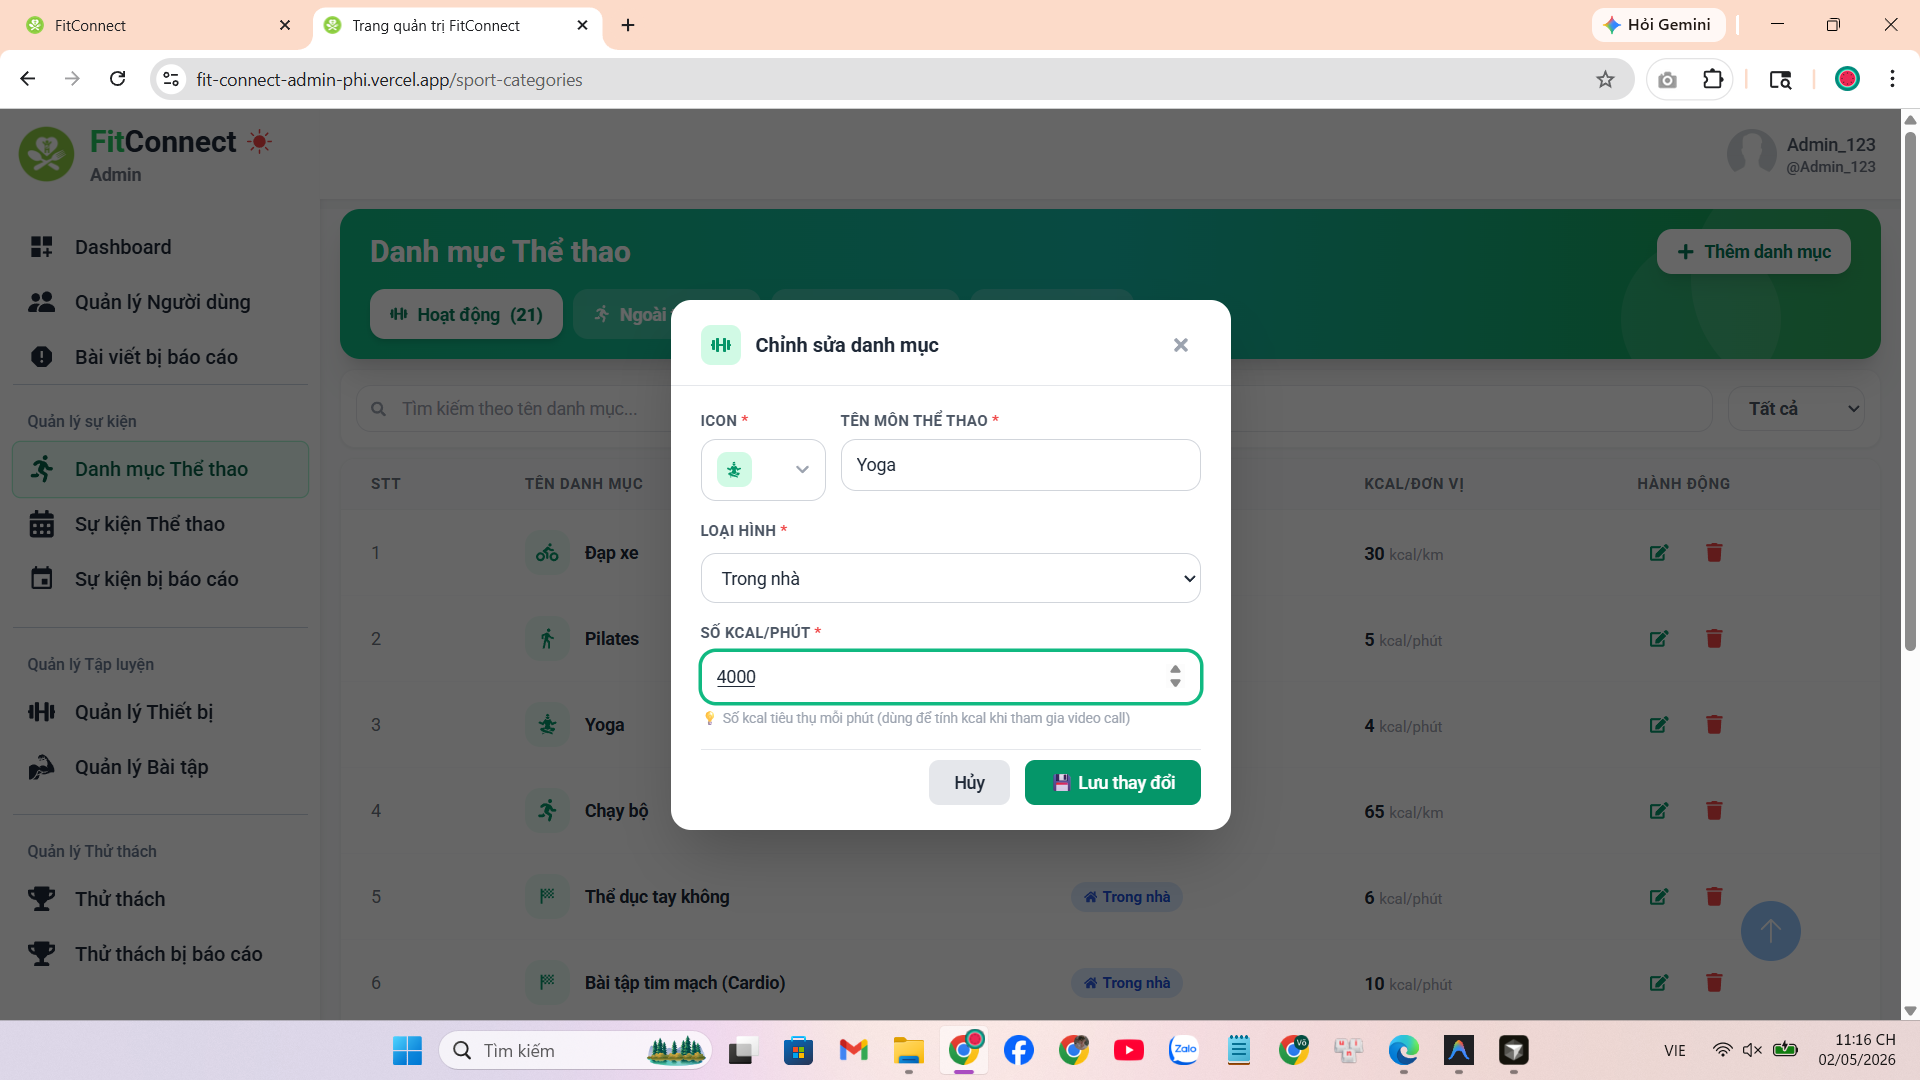
\includegraphics[width=\textwidth]{Images/IMG/nhom9/danhmucthethao/chinhsuathaydoisokcal.png}
        \caption{Thay đổi hệ số Kcal của môn thể thao}
        \label{fig:impl_admin_category_edit_kcal}
    \end{subfigure}
    \vspace{0.3em}
    \caption{Cập nhật thông số danh mục thể thao. Sau khi lưu, hệ số Kcal mới áp dụng ngay cho toàn bộ hoạt động liên quan.}
    \label{fig:impl_admin_category_edit}
\end{figure}


    \item Hệ thống hỗ trợ cơ chế vô hiệu hóa (xóa mềm) các môn thể thao không còn được hỗ trợ. Việc vô hiệu hóa sẽ ẩn danh mục khỏi danh sách lựa chọn tạo hoạt động mới của người dùng, nhưng không làm ảnh hưởng tới các dữ liệu lịch sử đã được ghi nhận trước đó.

\begin{figure}[H]
    \centering
    \begin{subfigure}[b]{0.47\textwidth}
        \centering
        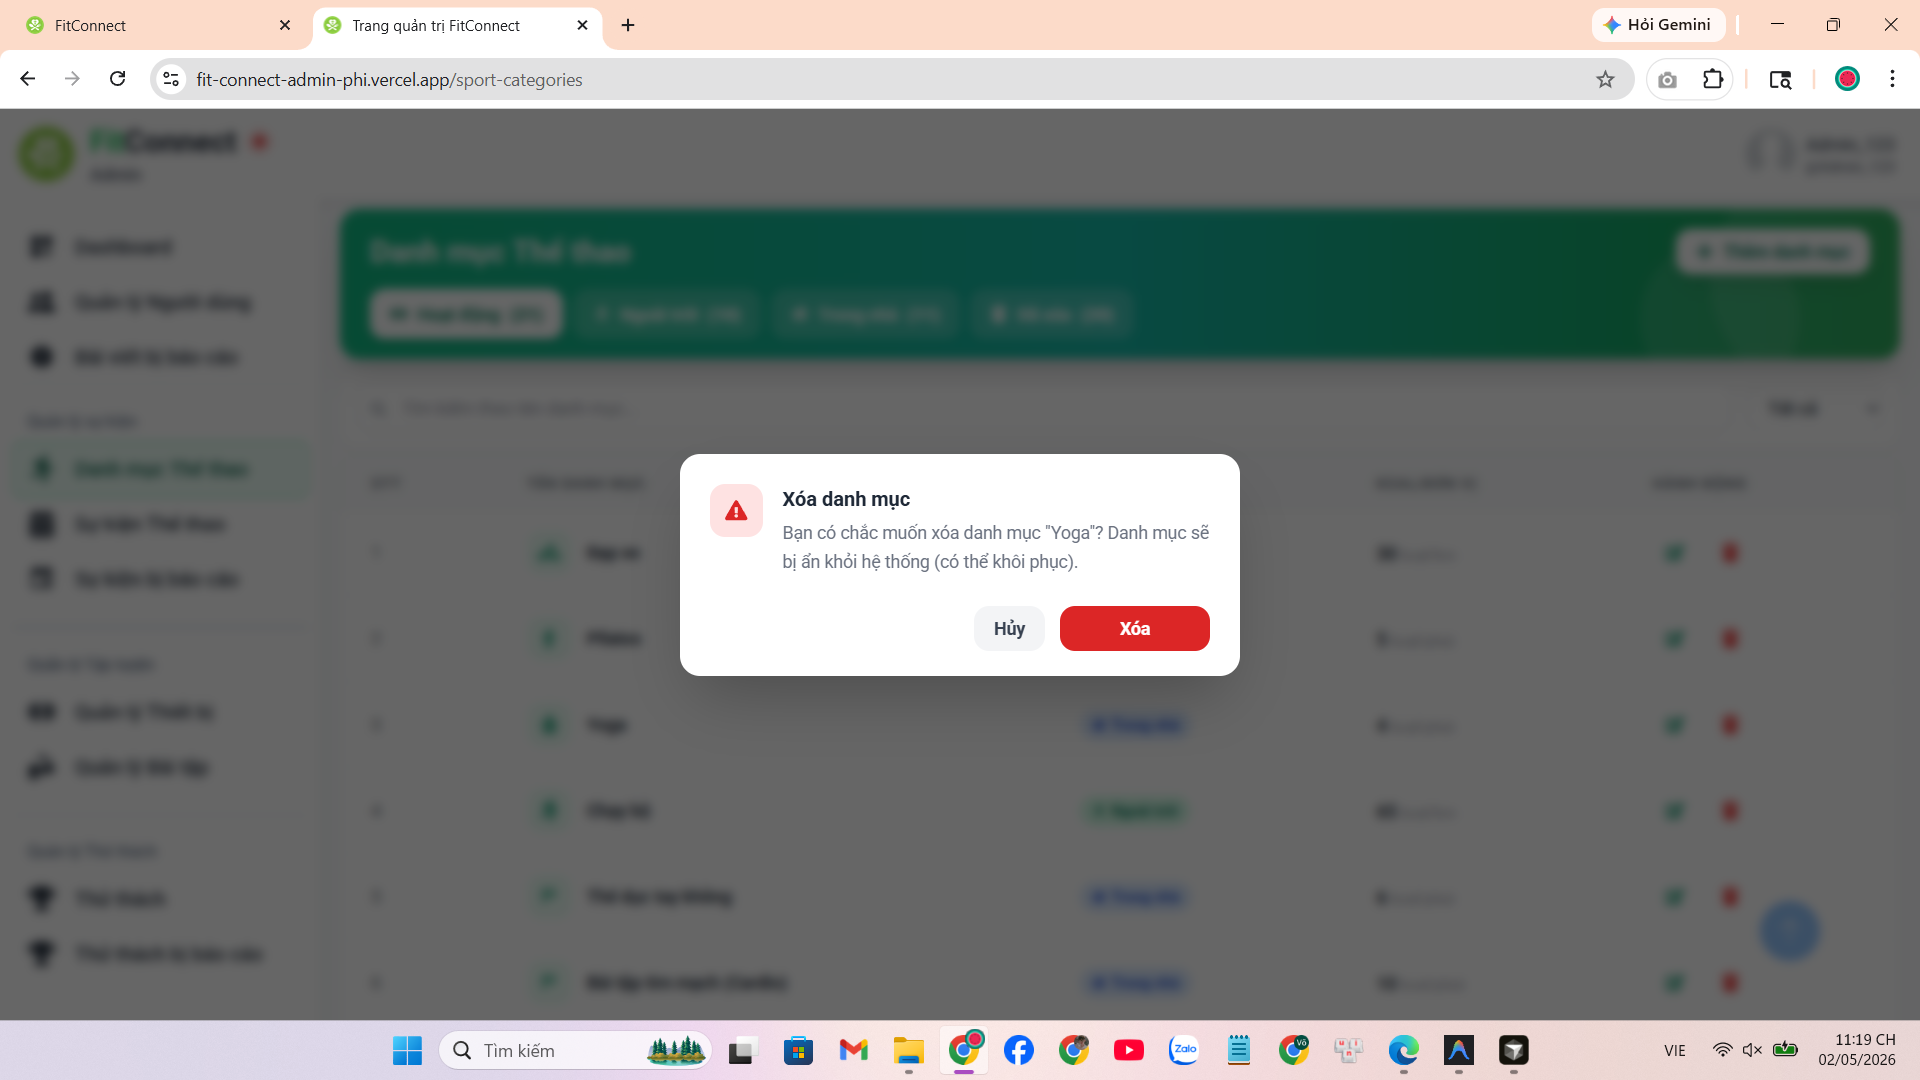
\includegraphics[width=\textwidth]{Images/IMG/nhom9/danhmucthethao/xoadanhmucyoga.png}
        \caption{Hệ thống hiển thị hộp thoại xác nhận vô hiệu hóa danh mục thể thao}
        \label{fig:impl_admin_category_delete}
    \end{subfigure}
    \hfill
    \begin{subfigure}[b]{0.47\textwidth}
        \centering
        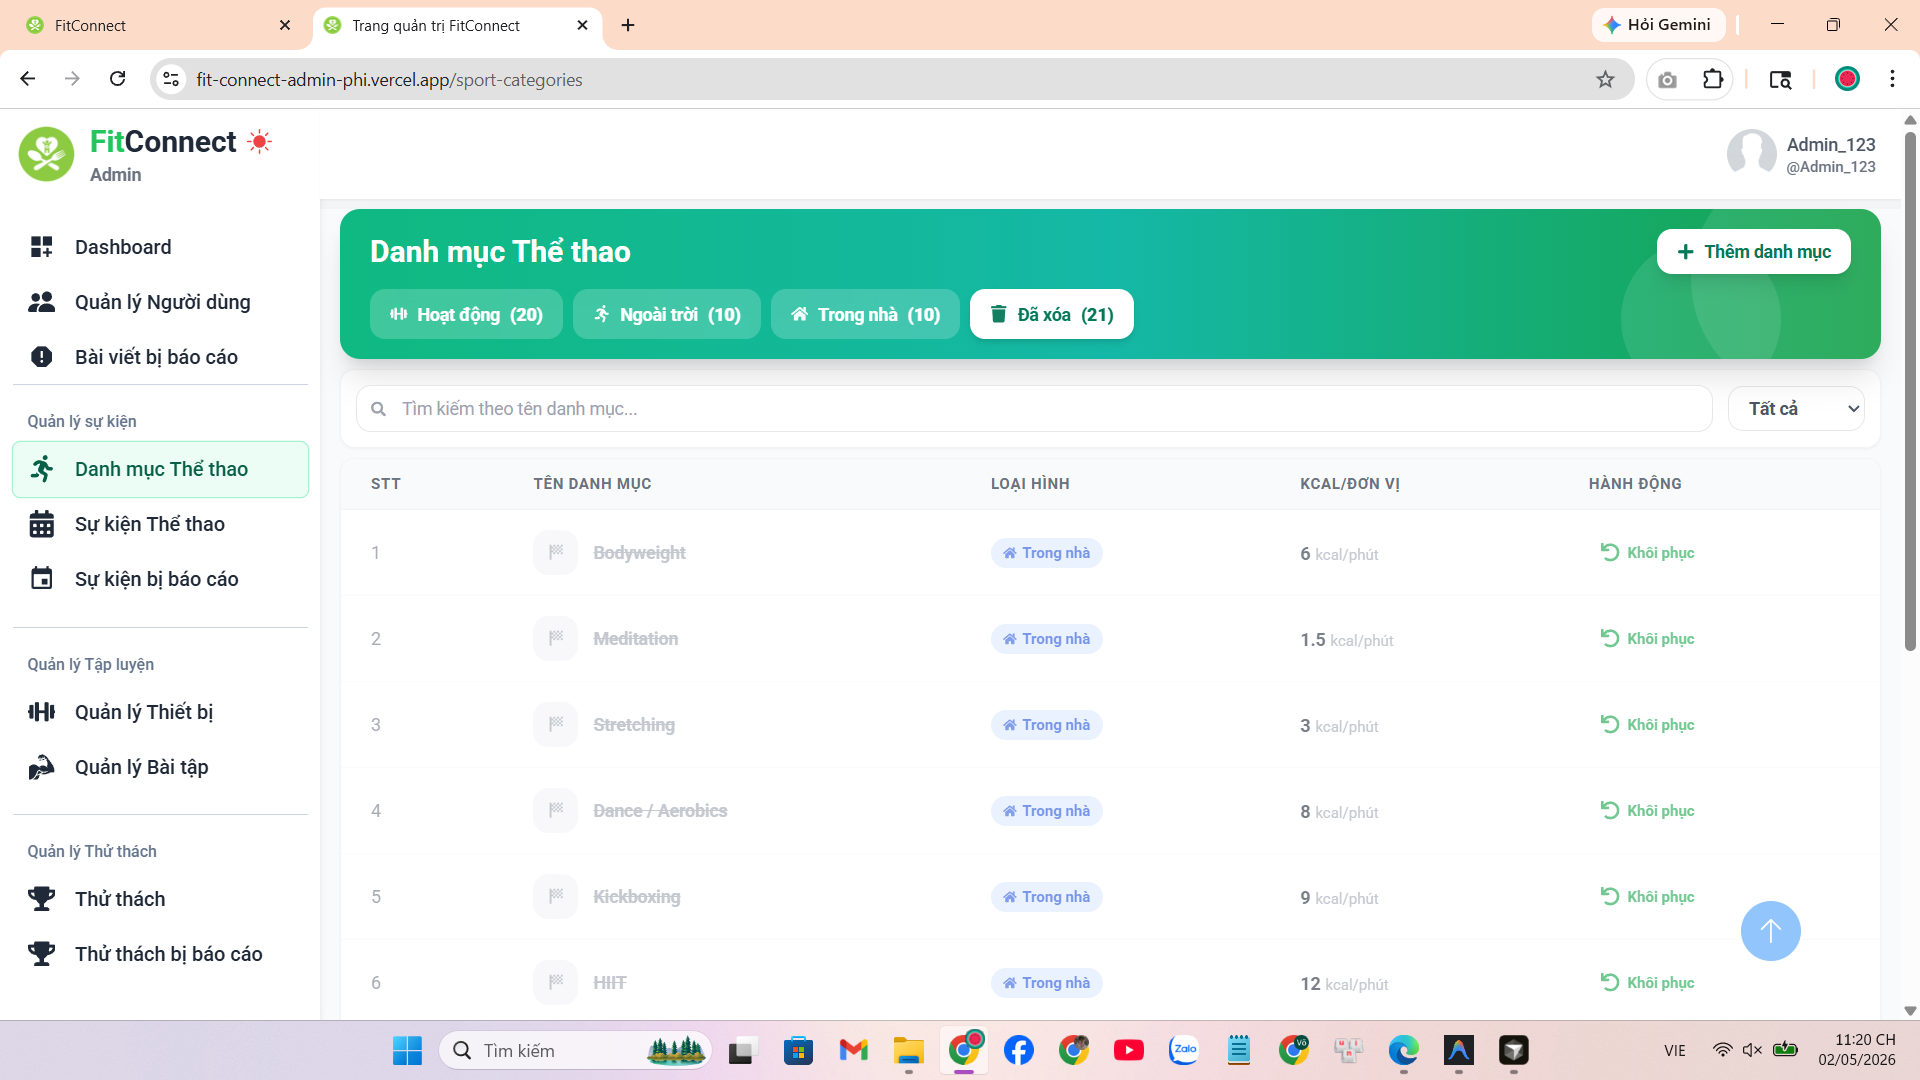
\includegraphics[width=\textwidth]{Images/IMG/nhom9/danhmucthethao/danhsachdanhmucdaxoa.png}
        \caption{Danh mục bị vô hiệu hóa được chuyển vào khu vực lưu trữ riêng biệt}
        \label{fig:impl_admin_category_deleted_list}
    \end{subfigure}
\end{figure}


    \item Các danh mục đã bị vô hiệu hóa có thể được khôi phục bất kỳ lúc nào. Sau khi khôi phục, danh mục hiển thị trở lại trong bảng cấu hình và sẵn sàng cho các hoạt động thể thao mới, đồng thời được tái tích hợp vào các sự kiện/thử thách liên quan.

\end{itemize}

\subsubsection{Luồng thao tác quản lý sự kiện thể thao}
\begin{itemize}
    \item Hệ thống cung cấp cho Quản trị viên bảng điều khiển tổng quan về tất cả các sự kiện thể thao đang diễn ra trên nền tảng. Danh sách hiển thị chi tiết các thông tin quan trọng như phân loại sự kiện (Trong nhà/Ngoài trời), thời gian tổ chức, địa điểm, tiến độ hoàn thành mục tiêu tập thể, và số lượng thành viên tham gia.

\begin{figure}[H]
    \centering
    
\includegraphics[width=0.60\textwidth]{Images/IMG/nhom9/quanlysukienthethao/danhsachsukien.png}
    \caption{Quản trị viên xem danh sách tổng hợp các sự kiện thể thao}
    \label{fig:impl_admin_event_list}
\end{figure}


    \item Để kiểm duyệt nội dung, Quản trị viên có thể xem phân tích chi tiết của từng sự kiện thông qua hộp thoại hiển thị nhanh. Chức năng này giúp Admin đánh giá tính hợp lệ của mục tiêu đề ra (ví dụ: quãng đường cần đạt) cũng như nội dung mô tả của người tổ chức.

\begin{figure}[H]
    \centering
    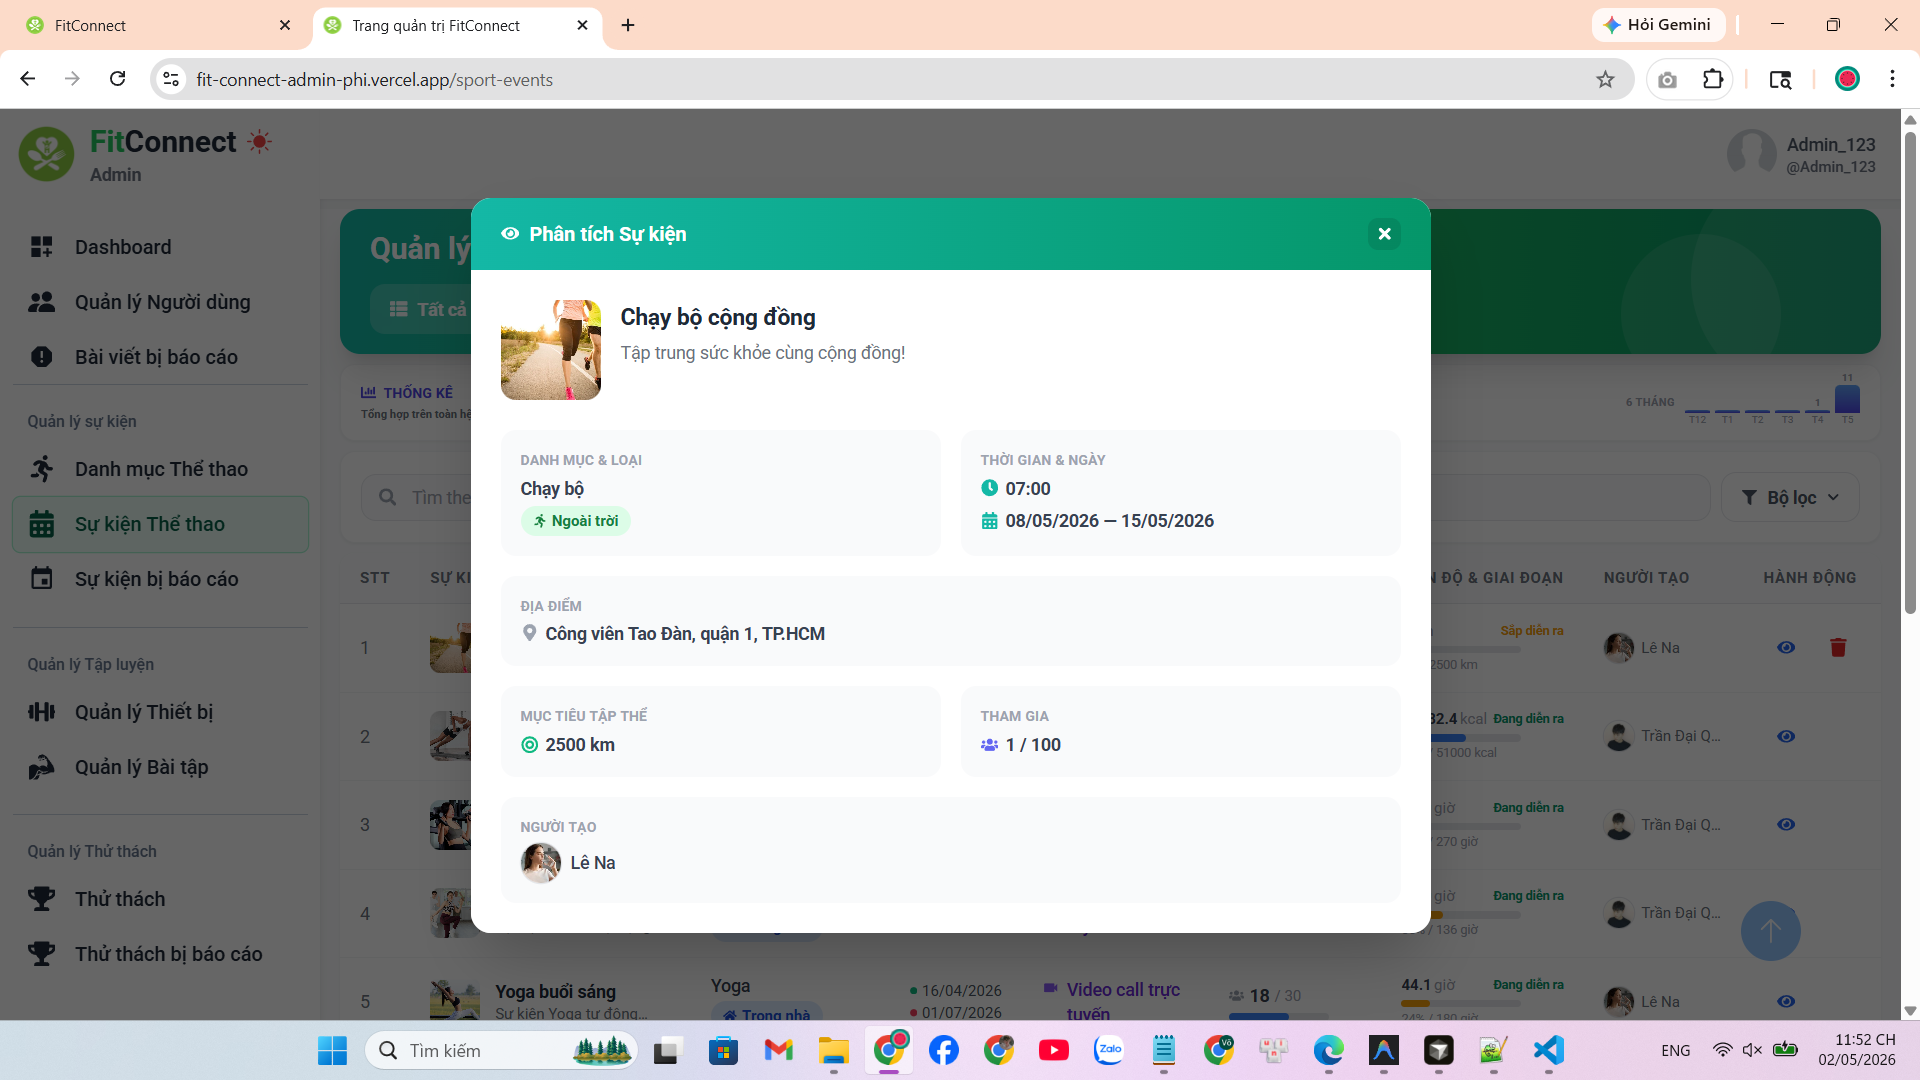
\includegraphics[width=0.60\textwidth]{Images/IMG/nhom9/quanlysukienthethao/xemthongtinsukien.png}
    \caption{Hệ thống hiển thị hộp thoại phân tích chi tiết thông tin sự kiện}
    \label{fig:impl_admin_event_detail}
\end{figure}


    \item Trong trường hợp phát hiện sự kiện vi phạm tiêu chuẩn cộng đồng hoặc chứa thông tin sai lệch, Quản trị viên có quyền can thiệp vô hiệu hóa sự kiện. Hệ thống sẽ yêu cầu xác nhận để tránh các thao tác sai lầm do vô ý.

\begin{figure}[H]
    \centering
    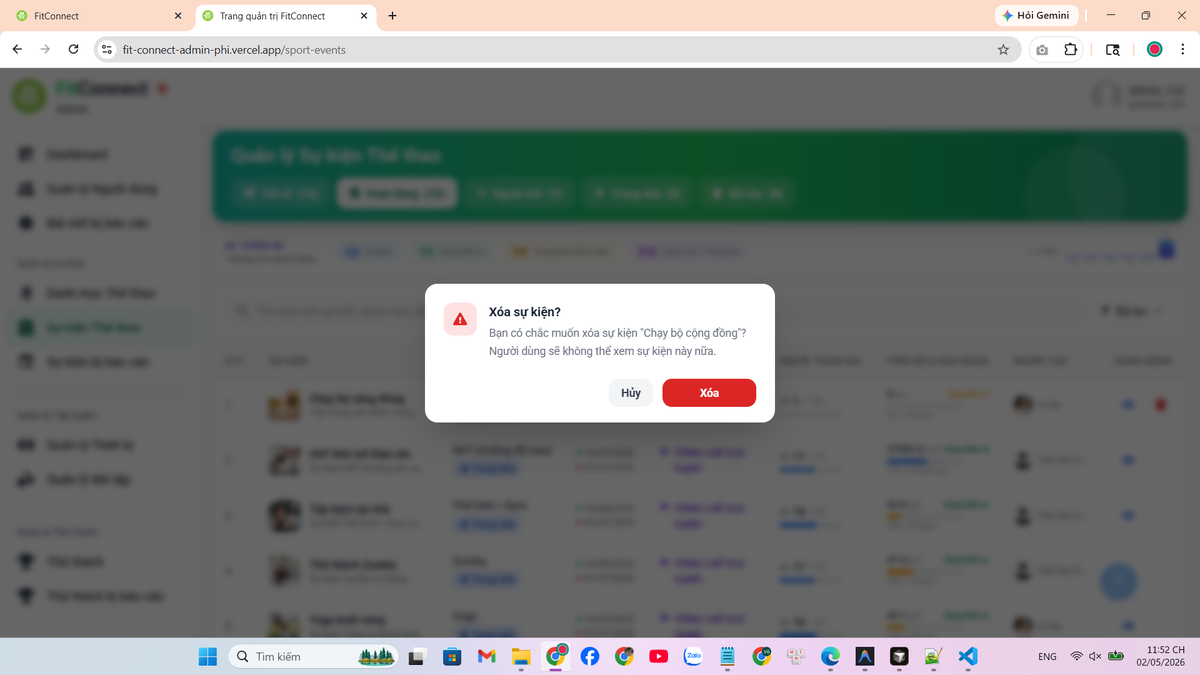
\includegraphics[width=0.60\textwidth]{Images/IMG/nhom9/quanlysukienthethao/modalxoasukien.png}
    \caption{Hệ thống hiển thị hộp thoại xác nhận vô hiệu hóa sự kiện}
    \label{fig:impl_admin_event_delete_confirm}
\end{figure}


    \item Khi sự kiện bị vô hiệu hóa, thay vì bị xóa hoàn toàn khỏi hệ thống, sự kiện sẽ được chuyển sang chế độ chỉ đọc (Read-only). Tại trạng thái này, người dùng vẫn có thể xem được các thông tin cơ bản và lịch sử của sự kiện nhưng mọi tính năng tương tác như tham gia, rời nhóm hay cập nhật tiến độ đều bị vô hiệu hóa để đảm bảo tính minh bạch của dữ liệu.
% \begin{figure}[H]
%     \centering
%     
\includegraphics[width=0.8\textwidth]{Images/IMG/nhom3/sukiensaukhixoa.png}
%     \vspace{1em}
%     \caption{Giao diện sự kiện chuyển sang chế độ chỉ đọc sau khi bị Quản trị viên vô hiệu hóa}
%     \label{fig:impl_admin_event_readonly_view}
% \end{figure}

    \item Nhằm quản lý rủi ro và hỗ trợ xử lý khiếu nại, các sự kiện bị vô hiệu hóa không bị xóa vĩnh viễn mà được lưu trữ trong danh sách ``Đã xóa''. Tại đây, Quản trị viên có thể xem lại lịch sử và thực hiện thao tác khôi phục nếu xác định sự kiện hoàn toàn hợp lệ.

\begin{figure}[H]
    \centering
    \begin{subfigure}[b]{0.47\textwidth}
        \centering
        
\includegraphics[width=\textwidth]{Images/IMG/nhom9/quanlysukienthethao/danhsachsukiendaxoa.png}
        \caption{Các sự kiện bị vô hiệu hóa được hệ thống lưu trữ tại danh mục riêng}
        \label{fig:impl_admin_event_deleted_list}
    \end{subfigure}
    \hfill
    \begin{subfigure}[b]{0.47\textwidth}
        \centering
        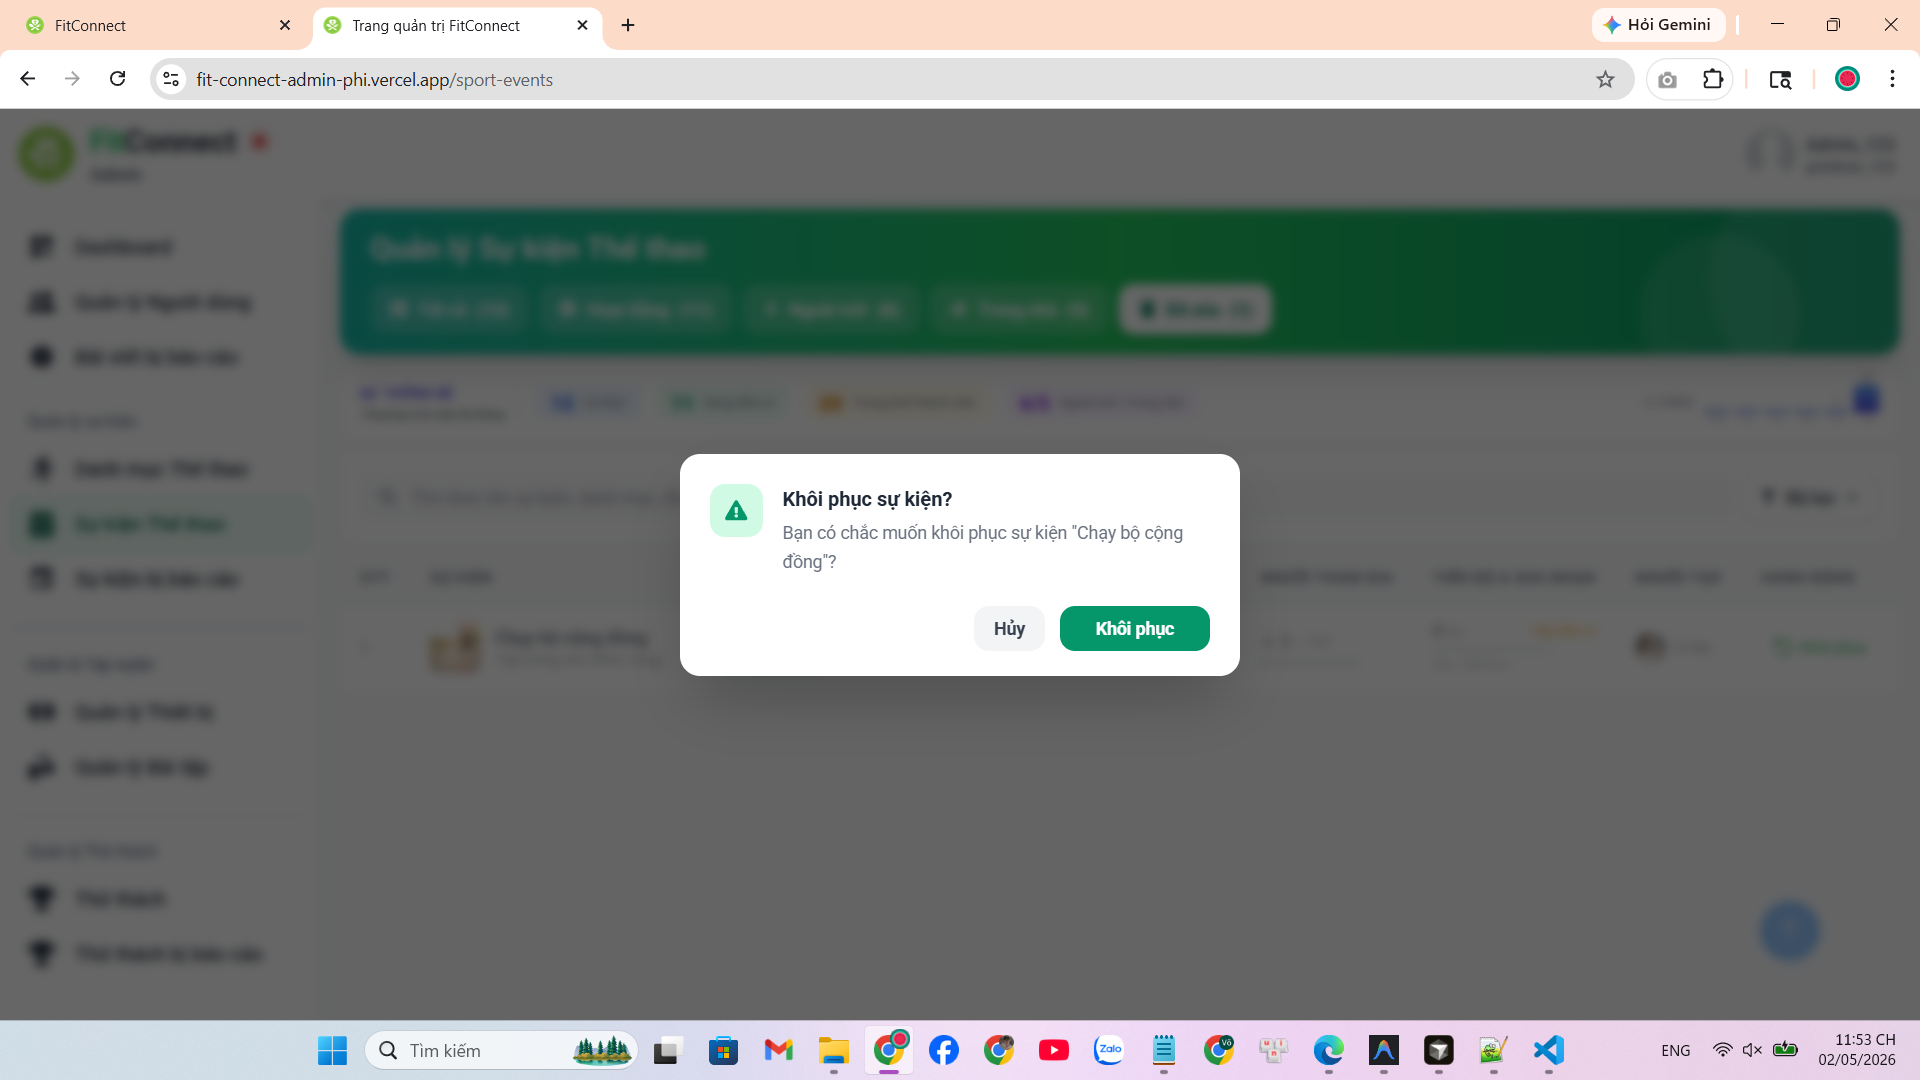
\includegraphics[width=\textwidth]{Images/IMG/nhom9/quanlysukienthethao/khoiphucsukien.png}
        \caption{Hệ thống hiển thị hộp thoại xác nhận khôi phục sự kiện}
        \label{fig:impl_admin_event_restore_confirm}
    \end{subfigure}
\end{figure}


    \item Sau khi khôi phục, sự kiện xuất hiện trở lại trên danh sách hoạt động chung. Mọi liên kết, tiến độ và danh sách người tham gia được bảo toàn nguyên vẹn, cho phép người dùng tiếp tục tương tác bình thường.

\end{itemize}

\subsubsection{Luồng thao tác kiểm duyệt sự kiện thể thao}
\begin{itemize}
    \item Tương tự cơ chế kiểm duyệt bài viết cộng đồng, hệ thống cung cấp tính năng báo cáo dành cho người dùng khi phát hiện các sự kiện thể thao có dấu hiệu gian lận, nội dung phản cảm hoặc vi phạm tiêu chuẩn nền tảng. Người dùng có thể cung cấp lý do chi tiết để hỗ trợ quá trình xử lý của Quản trị viên.

\begin{figure}[H]
    \centering
    \begin{subfigure}[b]{0.47\textwidth}
        \centering
        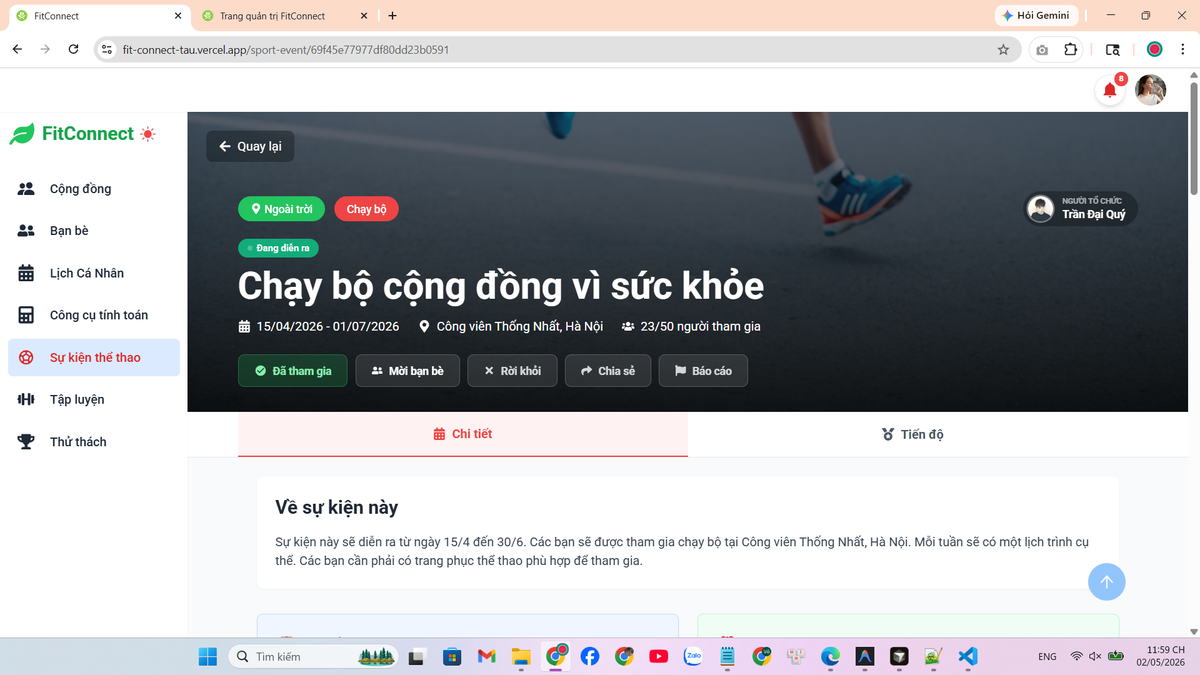
\includegraphics[width=\textwidth]{Images/IMG/nhom9/kiemduyetsukienthethao/sukienbenUser.png}
        \caption{Người dùng tương tác với sự kiện trên ứng dụng}
        \label{fig:impl_admin_event_mod_user_view}
    \end{subfigure}
    \hfill
    \begin{subfigure}[b]{0.47\textwidth}
        \centering
        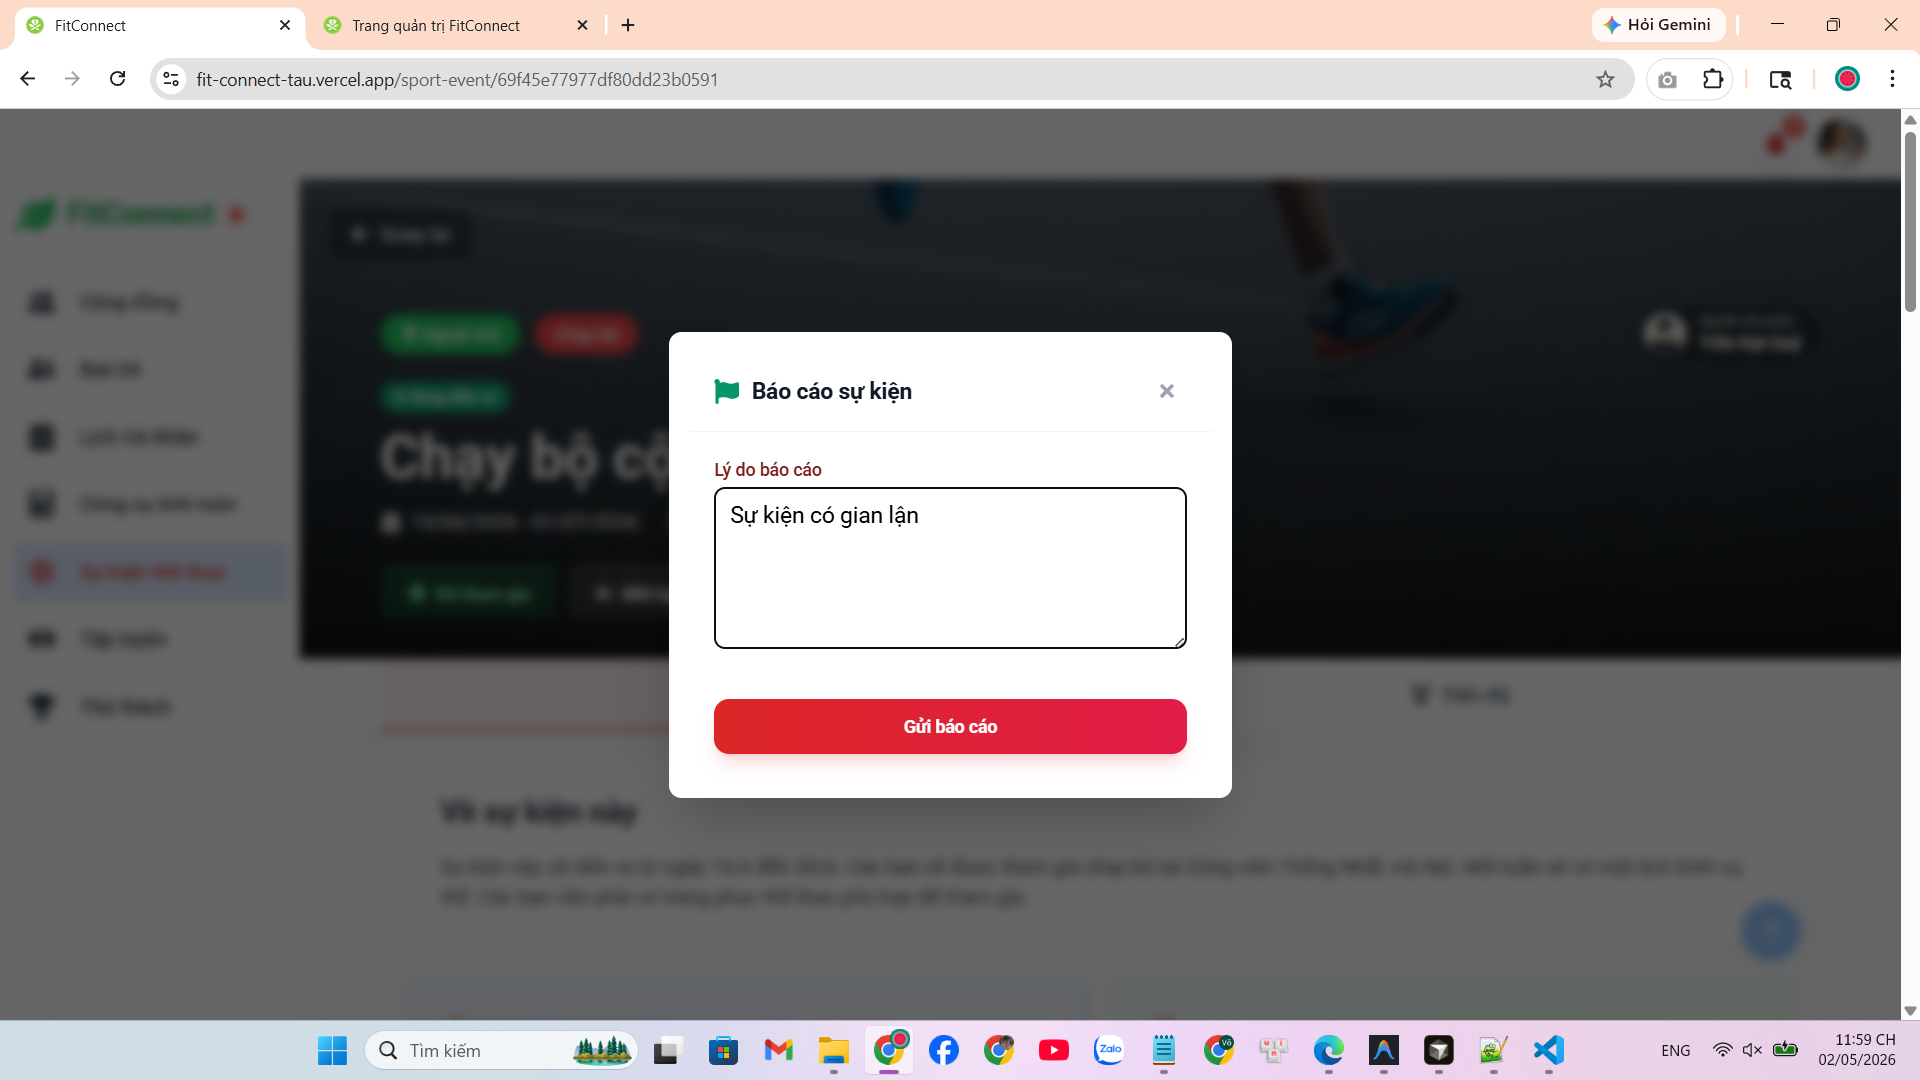
\includegraphics[width=\textwidth]{Images/IMG/nhom9/kiemduyetsukienthethao/Nguoidungbaocaosukien.png}
        \caption{Người dùng gửi báo cáo vi phạm đối với một sự kiện thể thao}
        \label{fig:impl_admin_event_mod_user_report}
    \end{subfigure}
\end{figure}


    \item Tại trang quản trị, các sự kiện bị báo cáo được tổng hợp thành một danh sách chờ xử lý. Giao diện cung cấp đầy đủ thông tin về người tạo, tên sự kiện, tổng số lượt báo cáo, thông tin người báo cáo và nội dung vi phạm bị cáo buộc.

\begin{figure}[H]
    \centering
    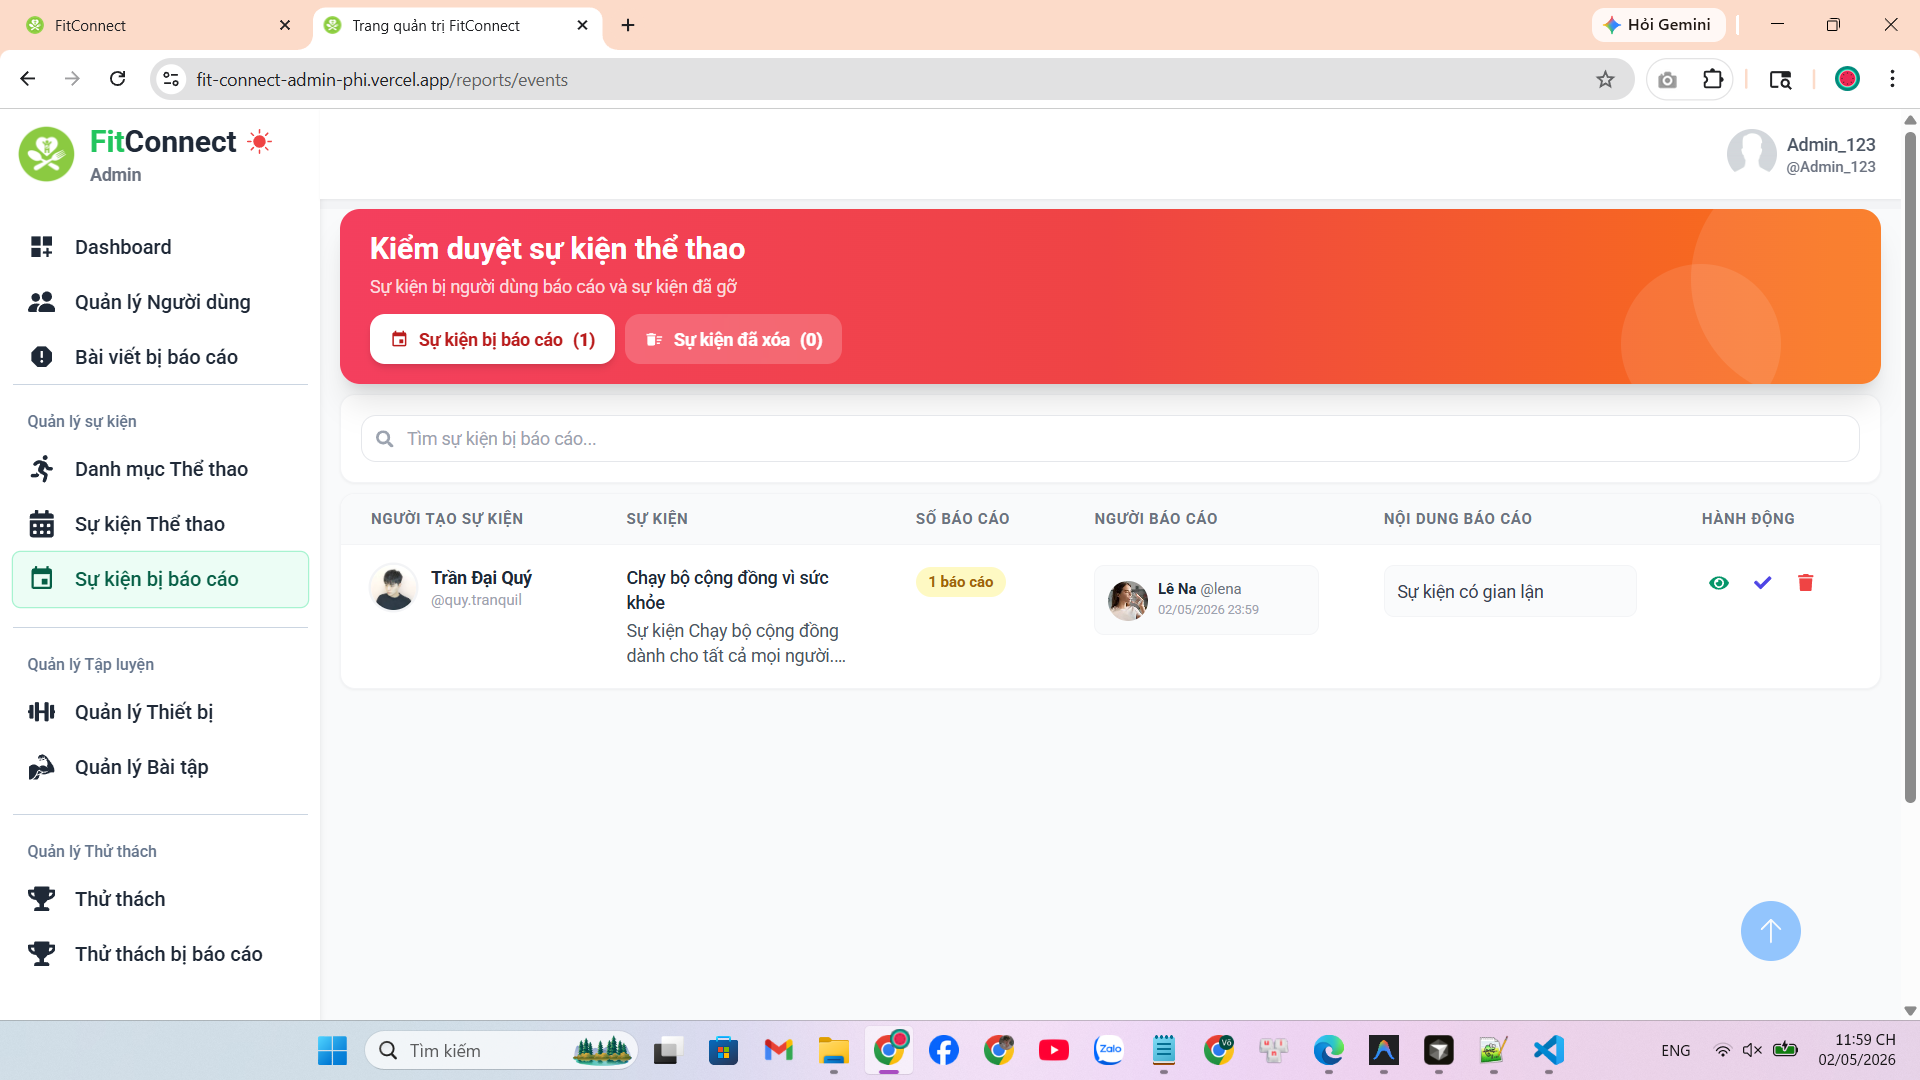
\includegraphics[width=0.60\textwidth]{Images/IMG/nhom9/kiemduyetsukienthethao/danhsachsukienbibaocaoadmin.png}
    \caption{Quản trị viên theo dõi danh sách các sự kiện thể thao bị báo cáo}
    \label{fig:impl_admin_event_mod_reported_list}
\end{figure}


    \item Để đảm bảo tính khách quan trước khi ra quyết định, Quản trị viên có thể xem chi tiết sự kiện kết hợp với nội dung khiếu nại thông qua một hộp thoại tích hợp.

\begin{figure}[H]
    \centering
    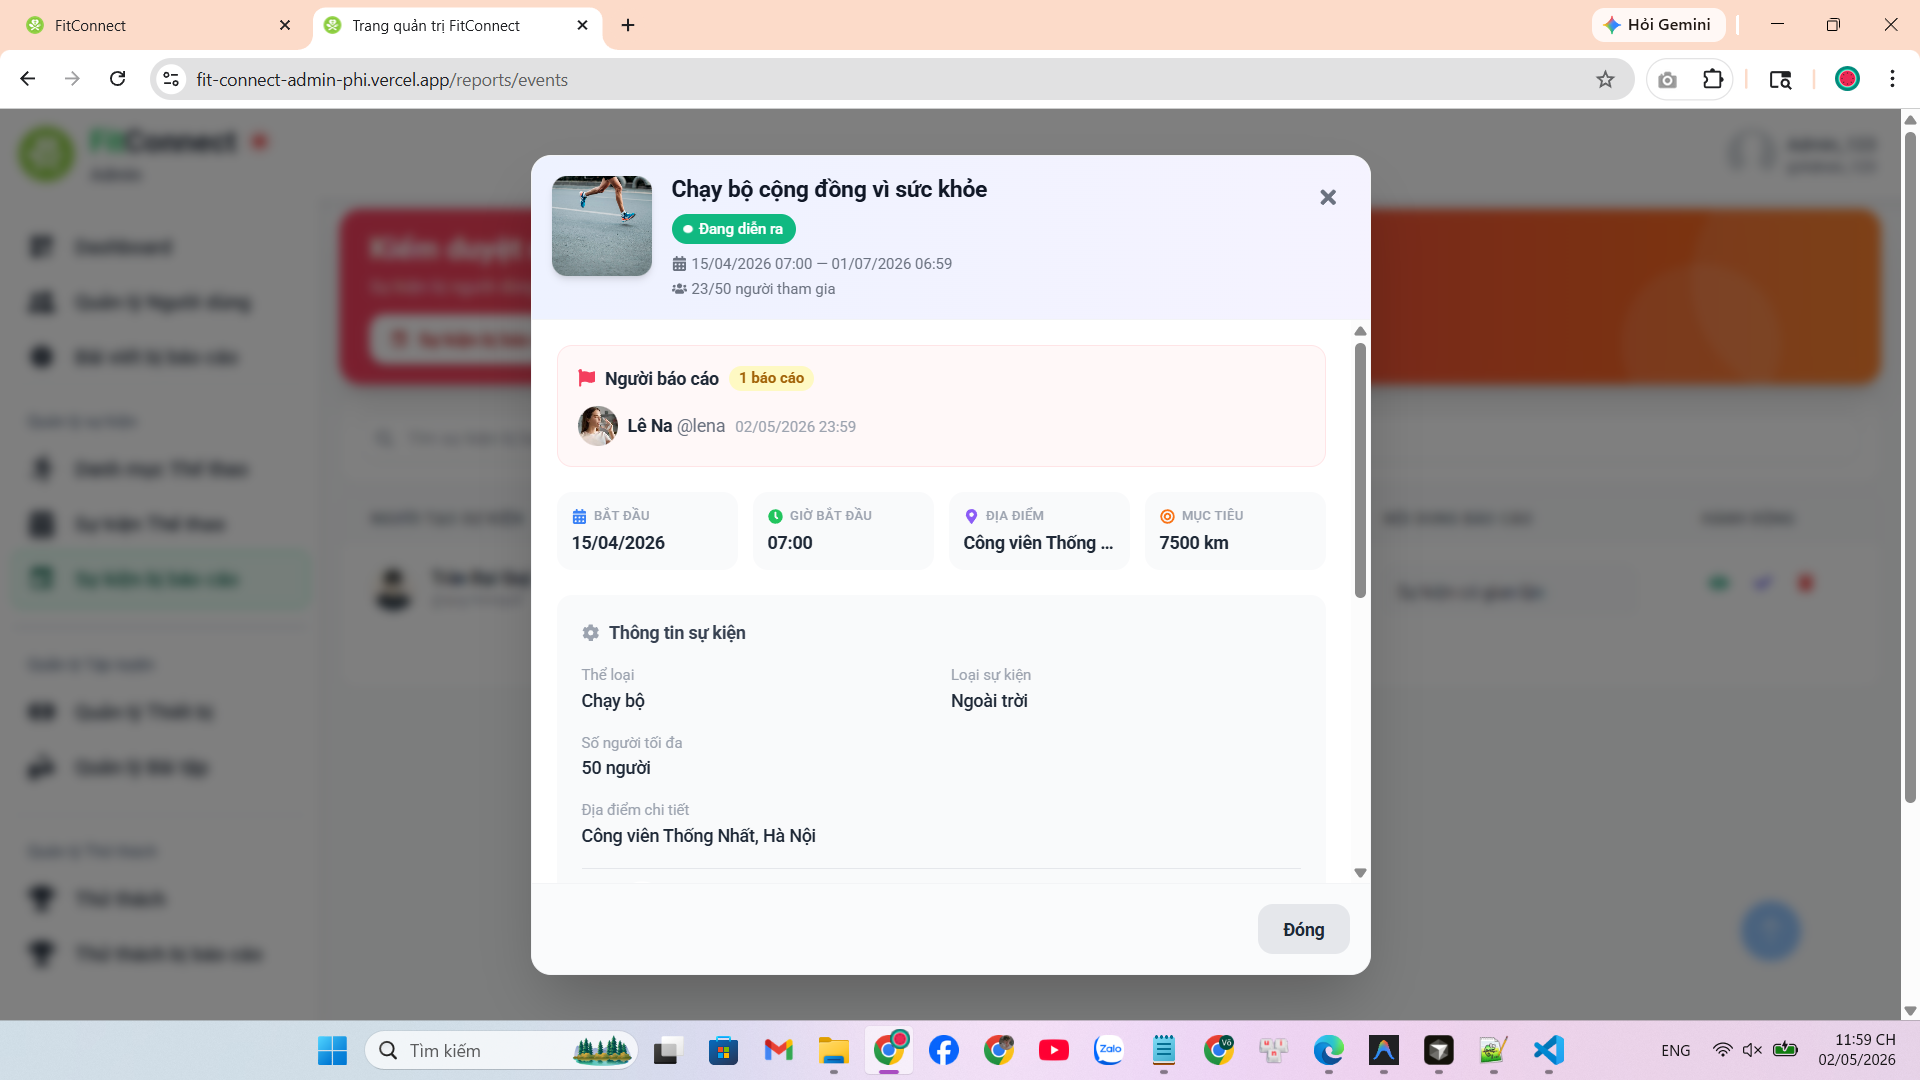
\includegraphics[width=0.60\textwidth]{Images/IMG/nhom9/kiemduyetsukienthethao/xemthongtinsukienbibaocao.png}
    \caption{Hệ thống hiển thị hộp thoại phân tích chi tiết sự kiện bị báo cáo}
    \label{fig:impl_admin_event_mod_detail}
\end{figure}


    \item Dựa trên xác minh, Admin quyết định \textbf{Giữ sự kiện} (bác bỏ báo cáo, xóa lịch sử khiếu nại) hoặc \textbf{Gỡ bỏ} (vô hiệu hóa sự kiện vi phạm, chuyển vào kho lưu trữ).

\begin{figure}[H]
    \centering
    \begin{subfigure}[b]{0.47\textwidth}
        \centering
        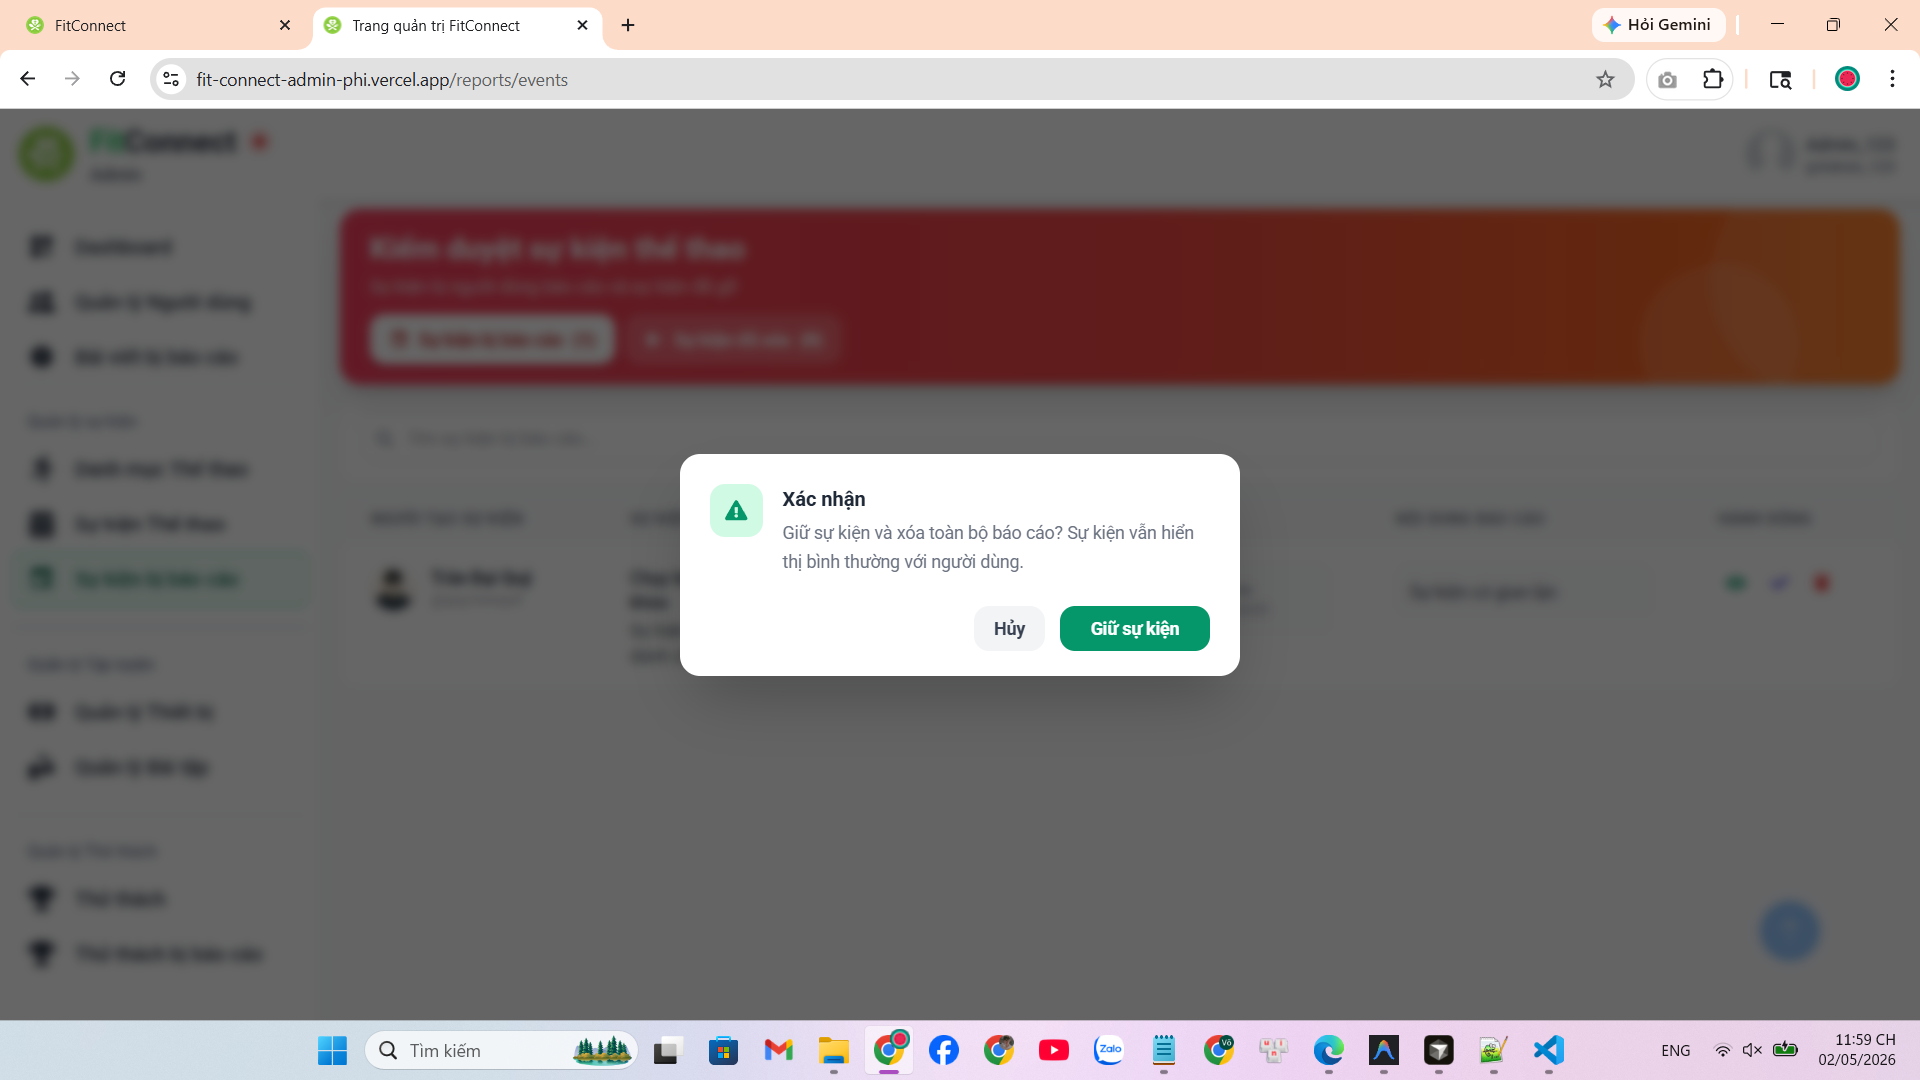
\includegraphics[width=\textwidth]{Images/IMG/nhom9/kiemduyetsukienthethao/modalgiusukien.png}
        \caption{Xác nhận giữ lại sự kiện hợp lệ}
        \label{fig:impl_admin_event_mod_keep}
    \end{subfigure}
    \hfill
    \begin{subfigure}[b]{0.47\textwidth}
        \centering
        
\includegraphics[width=\textwidth]{Images/IMG/nhom9/kiemduyetsukienthethao/adminxoasukien.png}
        \caption{Xác nhận gỡ bỏ sự kiện vi phạm}
        \label{fig:impl_admin_event_mod_remove}
    \end{subfigure}
    \vspace{0.3em}
    \caption{Hai hướng xử lý khi kiểm duyệt sự kiện bị báo cáo}
    \label{fig:impl_admin_event_mod_decision}
\end{figure}


    \item Việc gỡ bỏ sự kiện vi phạm sẽ khiến sự kiện ngay lập tức chuyển sang trạng thái hạn chế. Người dùng khi truy cập vào các sự kiện này sẽ nhận được thông báo về việc sự kiện đã bị quản trị viên gỡ bỏ và chuyển sang chế độ chỉ đọc, ngăn chặn mọi hành vi tương tác tiếp theo.
% \begin{figure}[H]
%     \centering
%     
\includegraphics[width=0.8\textwidth]{Images/IMG/nhom3/sukiensaukhixoa.png}
%     \vspace{1em}
%     \caption{Người dùng không thể thao tác với sự kiện đã bị gỡ bỏ do vi phạm}
%     \label{fig:impl_admin_event_mod_readonly_view}
% \end{figure}

    \item Mọi sự kiện bị gỡ bỏ đều được lưu trữ tại tab ``Đã xóa'' kèm thời điểm và nội dung vi phạm. Quản trị viên có thể khôi phục sự kiện bất kỳ lúc nào nếu cần thiết.

\begin{figure}[H]
    \centering
    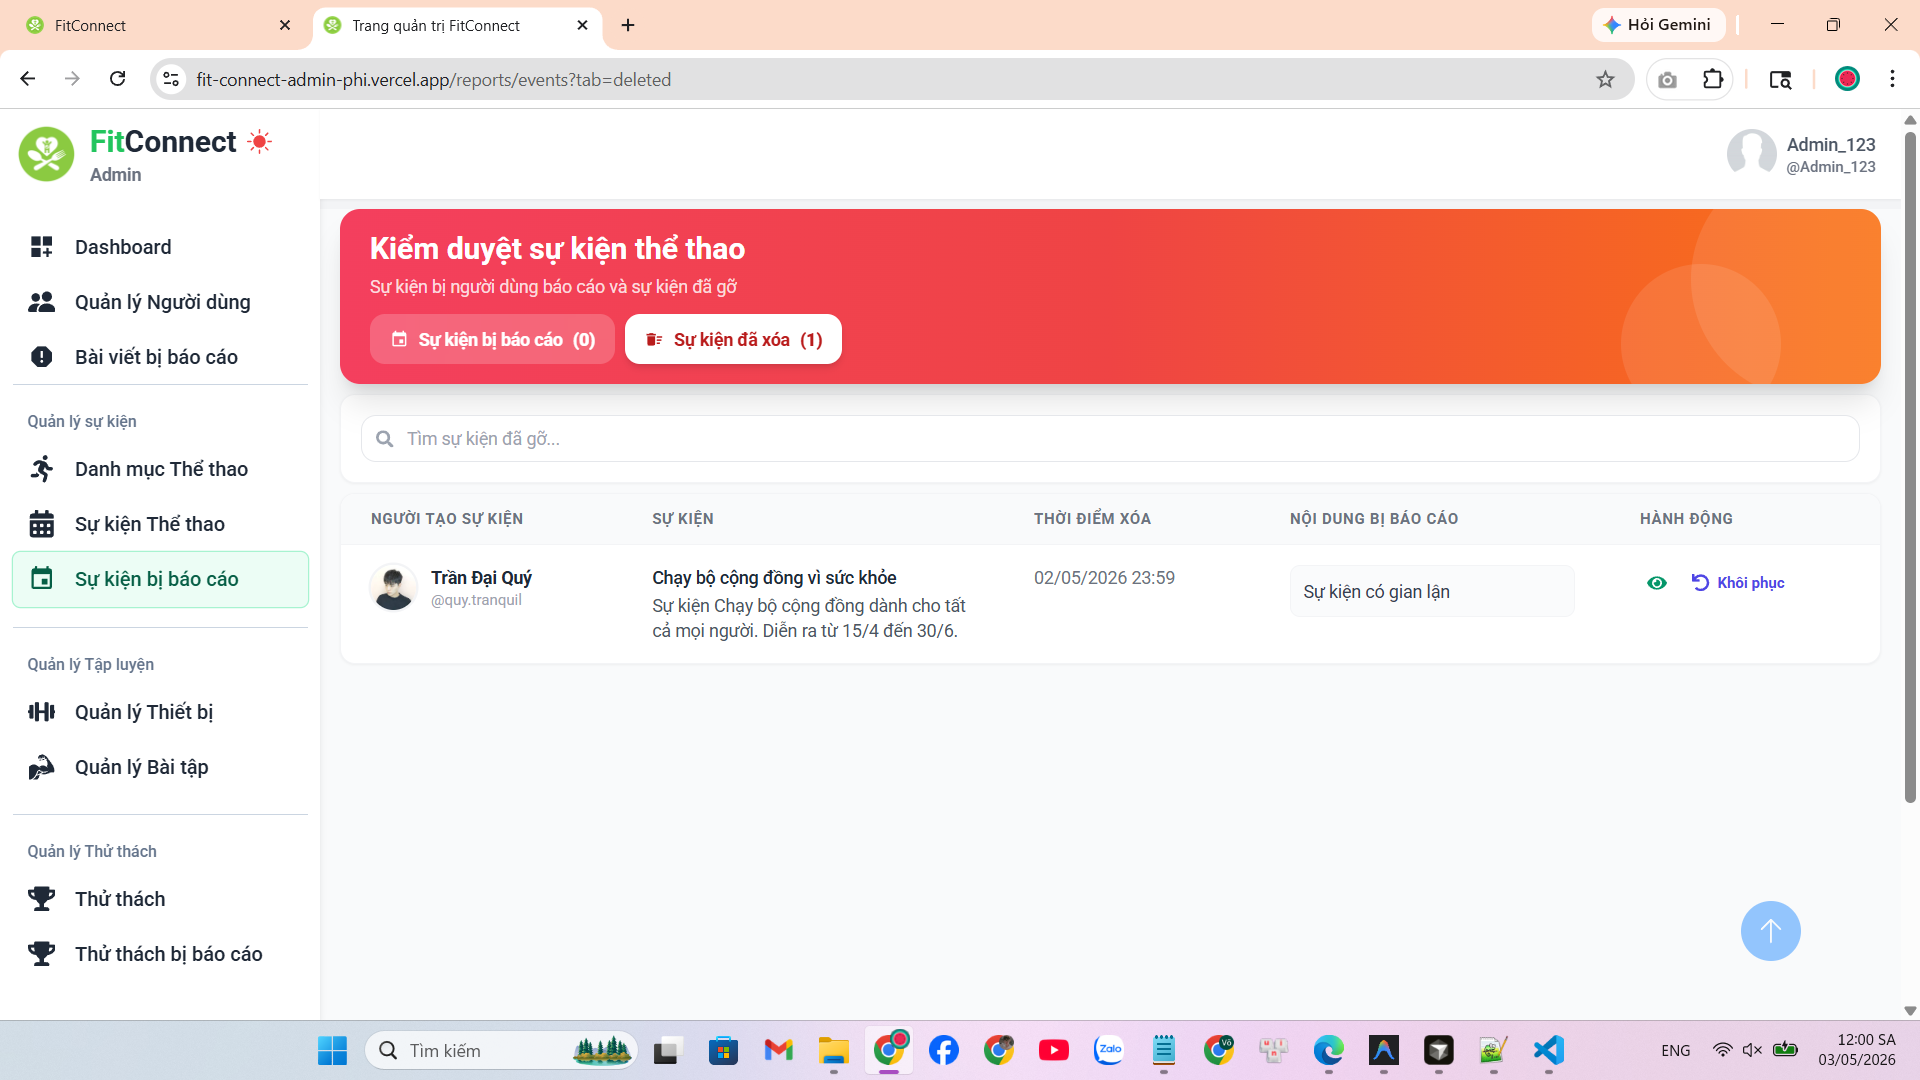
\includegraphics[width=0.60\textwidth]{Images/IMG/nhom9/kiemduyetsukienthethao/danhsachsukiendaxoa.png}
    \caption{Danh sách sự kiện đã bị gỡ bỏ do vi phạm, cho phép xem xét và khôi phục}
    \label{fig:impl_admin_event_mod_deleted_list}
\end{figure}

\end{itemize}

\subsubsection{Luồng thao tác quản lý thiết bị}
\begin{itemize}
    \item Trang Quản lý Thiết bị cho phép Quản trị viên xem và kiểm soát danh sách các loại thiết bị, dụng cụ hỗ trợ tập luyện có sẵn trong hệ thống (như xà đơn, ghế tập, tạ tay, tạ đòn, dây kháng lực,...). Giao diện hiển thị trực quan dưới dạng thẻ (card), cung cấp các thông tin cơ bản gồm hình ảnh minh họa, tên tiếng Việt, tên tiếng Anh, và trạng thái hiện tại (Hoạt động/Đã ẩn).

\begin{figure}[H]
    \centering
    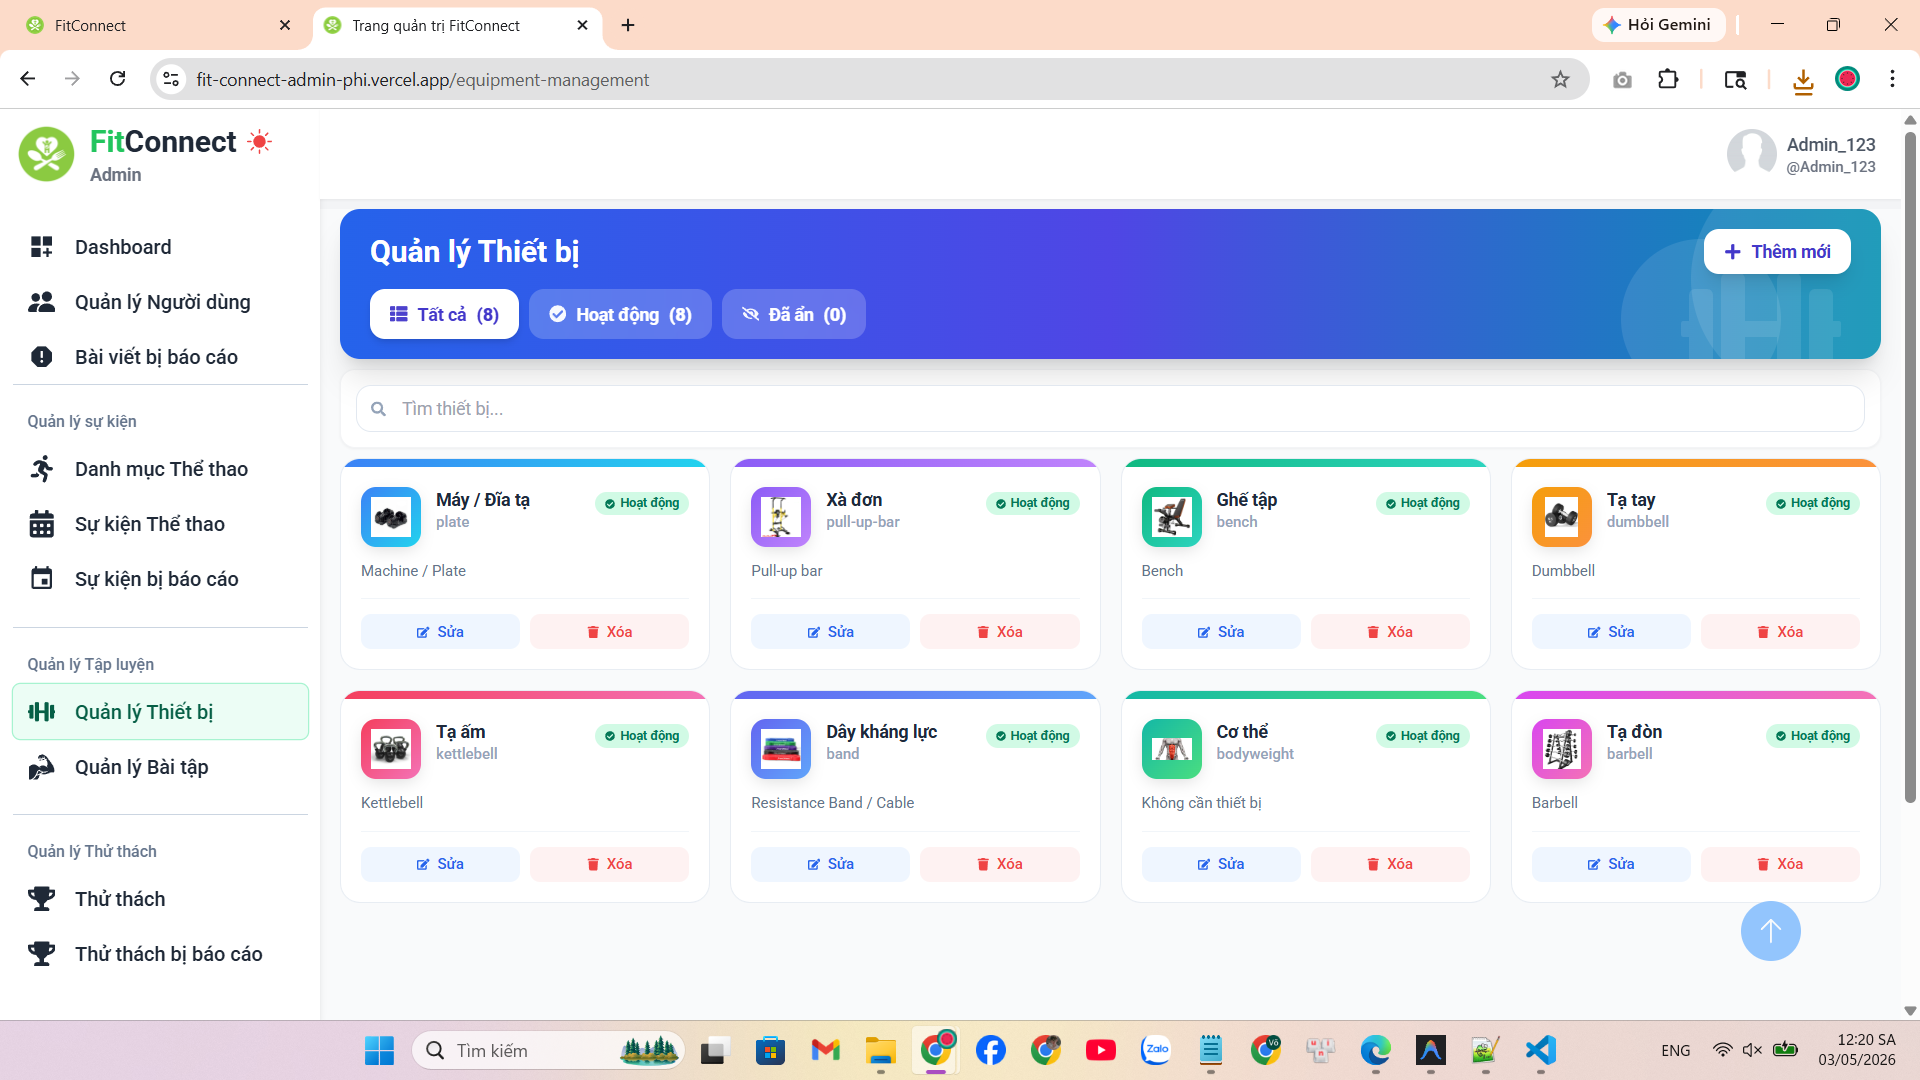
\includegraphics[width=0.60\textwidth]{Images/IMG/nhom9/quanlythietbi/danhsachthietbi.png}
    \caption{Giao diện danh sách các thiết bị tập luyện do hệ thống quản lý}
    \label{fig:impl_admin_equipment_list}
\end{figure}


    \item Để làm phong phú thêm cơ sở dữ liệu hỗ trợ tập luyện, Quản trị viên có thể sử dụng chức năng ``Thêm mới''. Hộp thoại Thêm thiết bị yêu cầu cung cấp hình ảnh minh họa định dạng chuẩn, tên gọi song ngữ (Anh - Việt), mô tả ngắn gọn và công tắc kích hoạt trạng thái hoạt động ngay lập tức.

\begin{figure}[H]
    \centering
    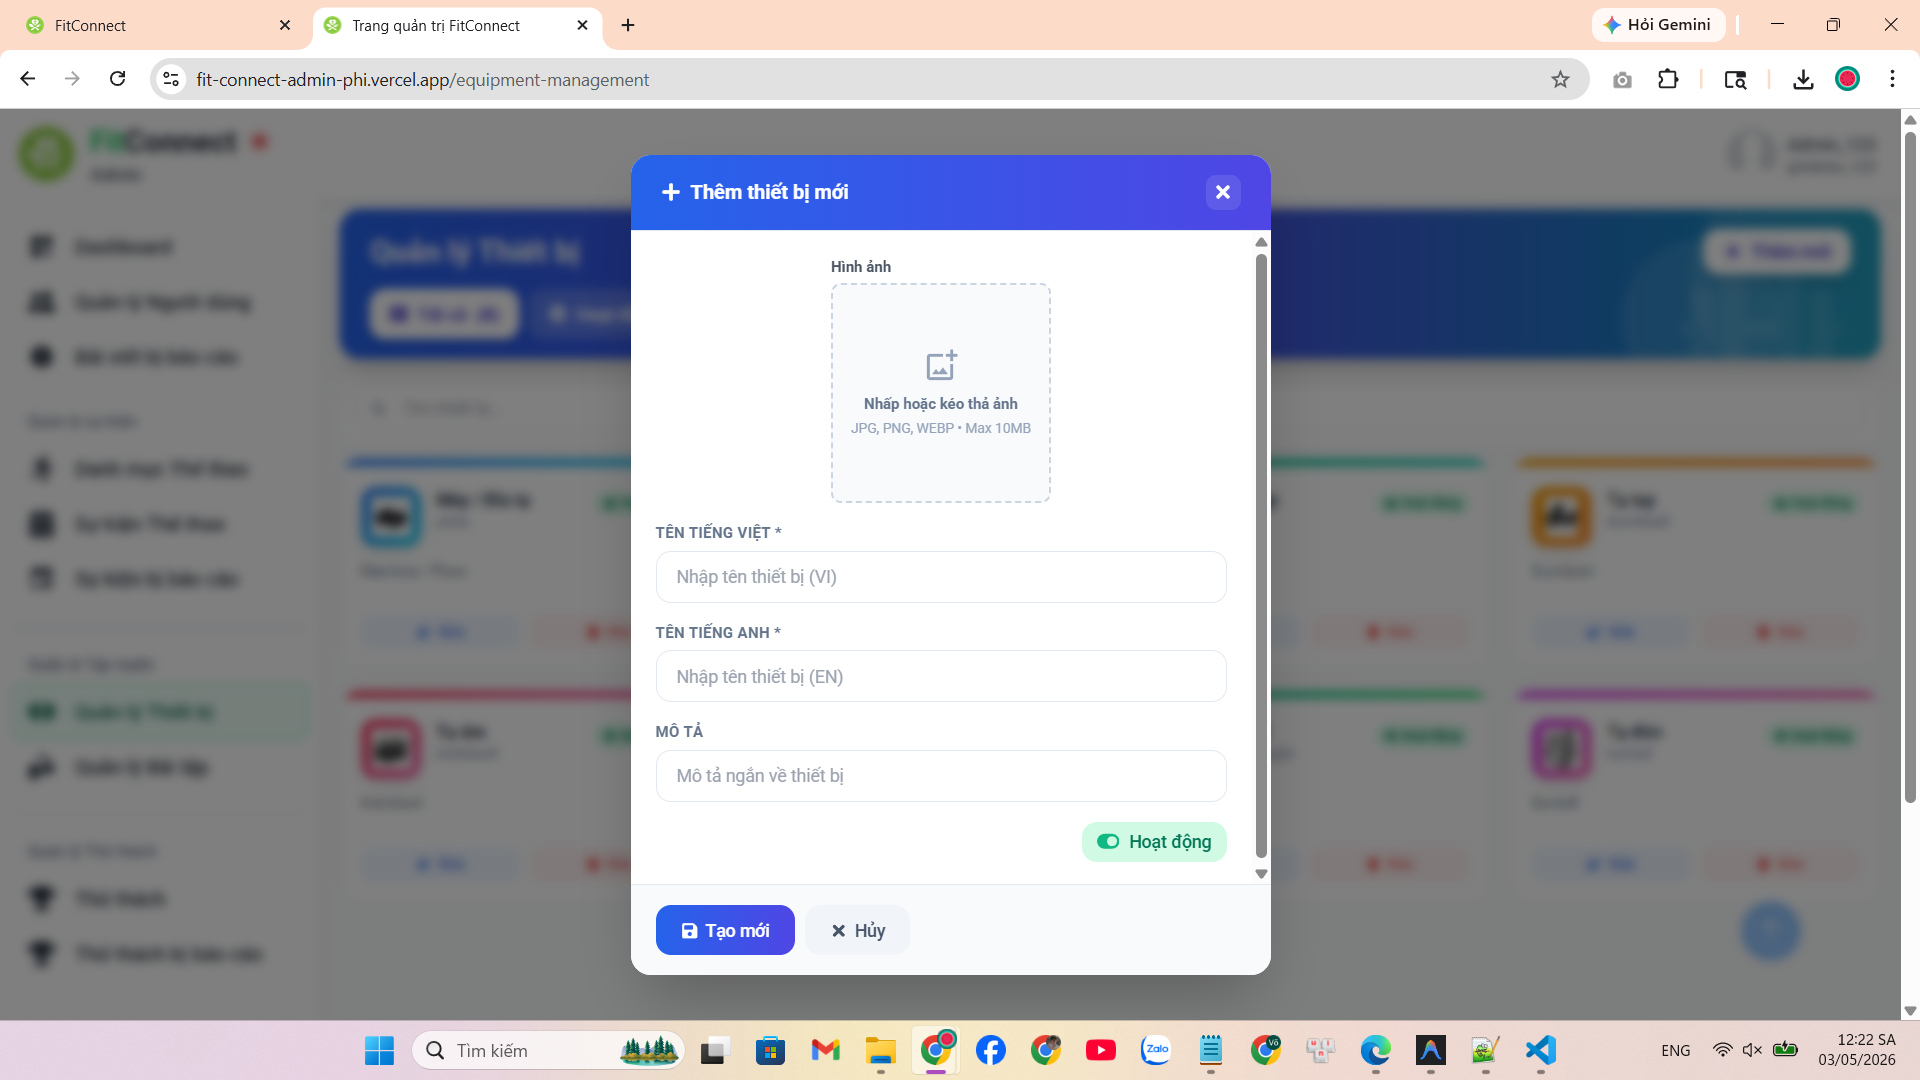
\includegraphics[width=0.60\textwidth]{Images/IMG/nhom9/quanlythietbi/themmoithietbi.png}
    \caption{Hệ thống cung cấp hộp thoại tạo mới thiết bị tập luyện}
    \label{fig:impl_admin_equipment_add}
\end{figure}


    \item Khi có sự thay đổi về thông tin (ví dụ: cần cập nhật hình ảnh rõ nét hơn hoặc bổ sung mô tả), tính năng ``Sửa'' cho phép Admin thực hiện cập nhật dựa trên form dữ liệu đã được điền sẵn. Mọi thay đổi đều được hệ thống lưu trữ đồng bộ, giúp dữ liệu thiết bị luôn chính xác khi liên kết với các bài tập.

\begin{figure}[H]
    \centering
    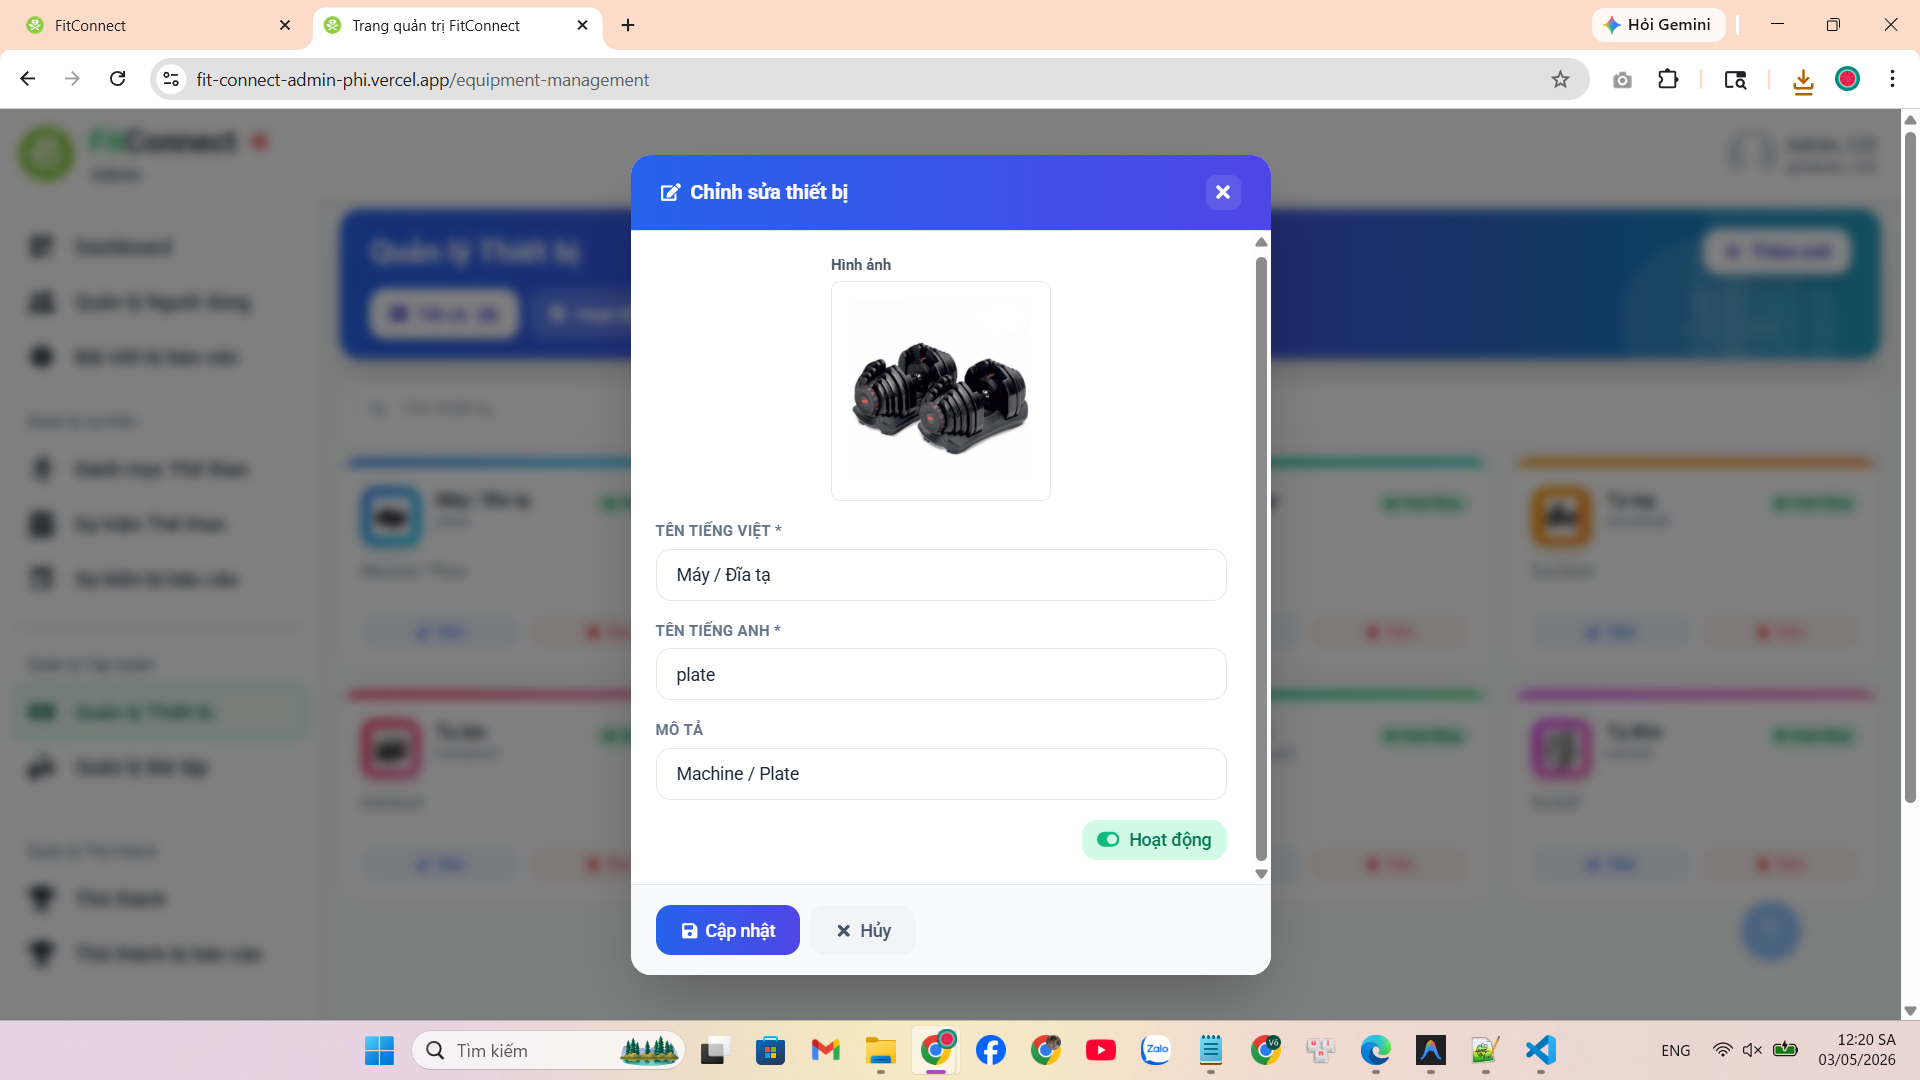
\includegraphics[width=0.60\textwidth]{Images/IMG/nhom9/quanlythietbi/chinhsuathietbi.png}
    \caption{Hộp thoại chỉnh sửa thông tin thiết bị với dữ liệu được điền sẵn}
    \label{fig:impl_admin_equipment_edit}
\end{figure}

\end{itemize}

\subsubsection{Luồng thao tác quản lý bài tập}
\begin{itemize}
    \item Trang Quản lý Bài tập là trung tâm kiểm soát toàn bộ cơ sở dữ liệu các động tác tập luyện (exercises). Giao diện cung cấp danh sách chi tiết dưới dạng bảng, phân loại theo loại hình (Sức mạnh, Tim mạch, Giãn cơ, Bật nhảy), độ khó, cấu trúc sets/reps, nhóm cơ chịu tác động và các thiết bị đi kèm. Tính năng bộ lọc (Filter) thông minh theo Nhóm cơ hoặc Thiết bị giúp Admin dễ dàng tra cứu khối lượng dữ liệu khổng lồ.

\begin{figure}[H]
    \centering
    
\includegraphics[width=0.60\textwidth]{Images/IMG/nhom9/quanlybaitap/danhsachbaitap.png}
    \caption{Giao diện tổng quan danh sách bài tập được phân loại chi tiết}
    \label{fig:impl_admin_exercise_list}
\end{figure}


    \item Quy trình thêm một bài tập mới đòi hỏi sự chính xác cao về chuyên môn. Hộp thoại ``Thêm bài tập mới'' không chỉ thu thập thông tin cơ bản (tên song ngữ, phân loại), mà còn yêu cầu thiết lập các cấu hình phức tạp: lựa chọn đa dạng các nhóm cơ và thiết bị bằng thẻ (tags), nhập hướng dẫn từng bước chi tiết, cung cấp liên kết video minh họa, cấu hình nhịp tập (số giây/rep, thời gian nghỉ) và đặc biệt là bảng thông số Set tập mặc định. Bảng này hỗ trợ tự động gợi ý chỉ số luyện tập tiêu chuẩn dựa trên mức độ khó (Dễ, Trung bình, Khó) với các giá trị về số rep, mức tạ và năng lượng Kcal tiêu thụ ước tính.

\begin{figure}[H]
    \centering
    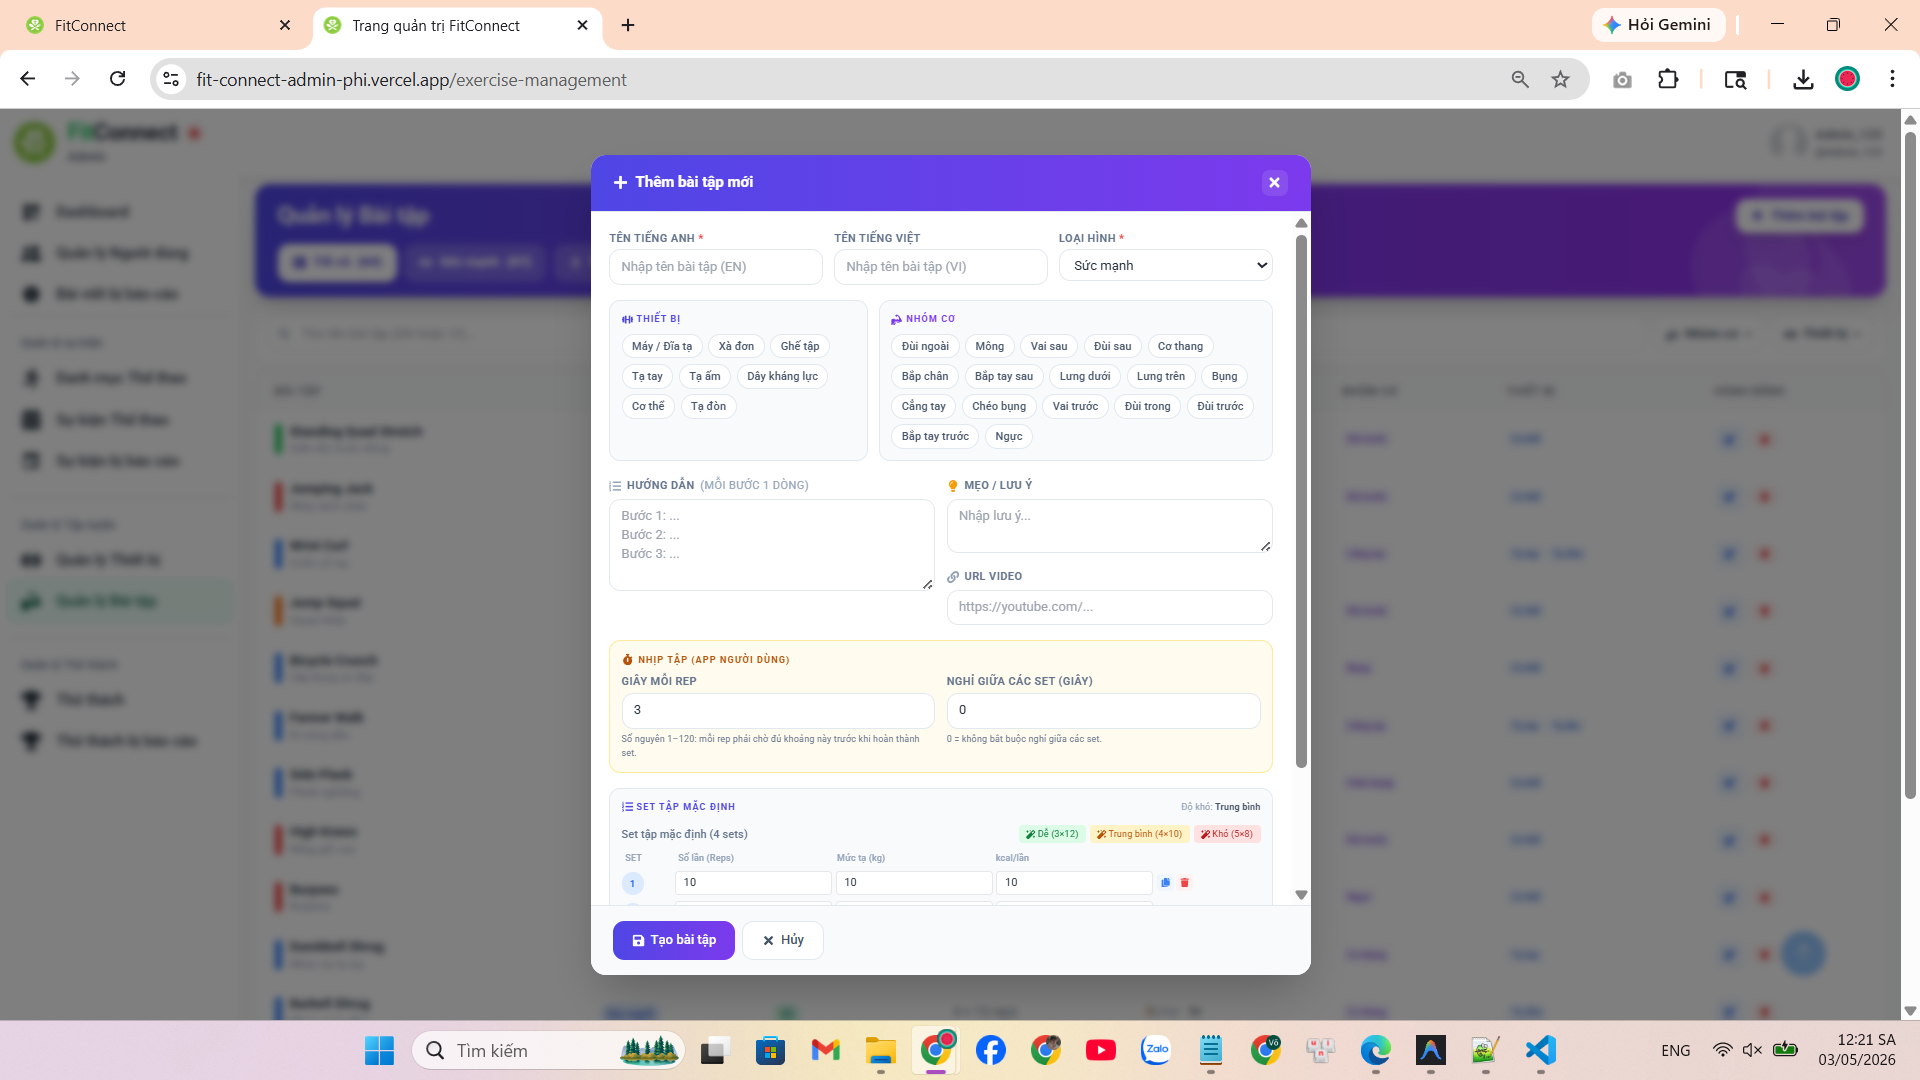
\includegraphics[width=0.60\textwidth]{Images/IMG/nhom9/quanlybaitap/themmoibaitap.png}
    \caption{Hộp thoại thêm mới bài tập với hệ thống thiết lập thông số chuyên sâu}
    \label{fig:impl_admin_exercise_add}
\end{figure}


    \item Trong trường hợp cần tinh chỉnh hướng dẫn tập luyện hoặc cập nhật chỉ số Kcal để phù hợp hơn với thực tế, chức năng chỉnh sửa cung cấp môi trường làm việc trực quan. Quản trị viên dễ dàng thêm/bớt nhóm cơ tác động hoặc sửa đổi lại cấu trúc từng set tập trước khi lưu cập nhật. Dữ liệu này sẽ làm nền tảng cốt lõi cho tính năng tự động thiết kế lộ trình tập luyện thông minh của người dùng (Smart Workout).

\begin{figure}[H]
    \centering
    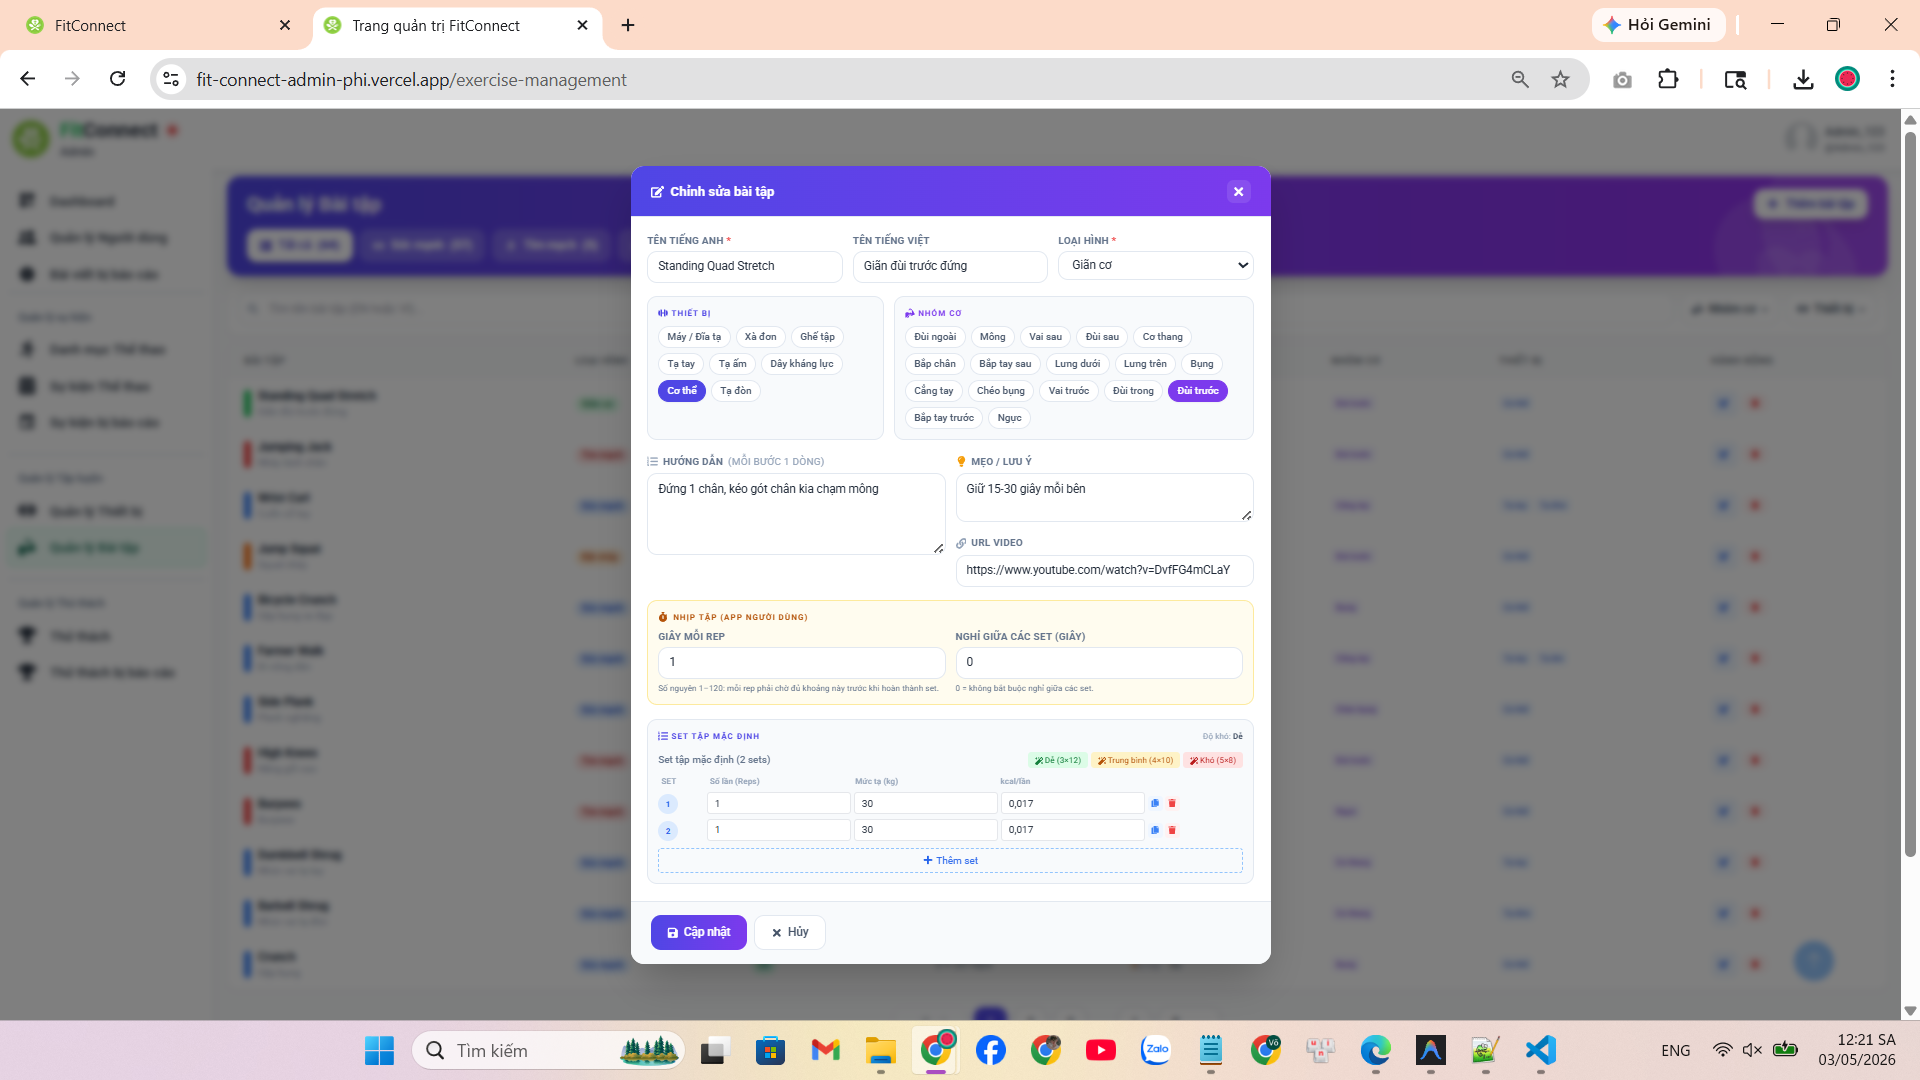
\includegraphics[width=0.60\textwidth]{Images/IMG/nhom9/quanlybaitap/chinhsuabaitap.png}
    \caption{Giao diện chỉnh sửa cho phép tinh chỉnh lại các thông số kỹ thuật của bài tập}
    \label{fig:impl_admin_exercise_edit}
\end{figure}

\end{itemize}

\subsubsection{Luồng thao tác quản lý thử thách}
\begin{itemize}
    \item Hệ thống cung cấp cho Quản trị viên giao diện quản lý tập trung toàn bộ các thử thách cộng đồng. Tại đây, Admin có thể theo dõi danh sách các thử thách đang hoạt động, bao gồm thông tin về loại thử thách (Sức mạnh, Tim mạch,...), số lượng người tham gia, thời gian bắt đầu và kết thúc, cùng trạng thái hiện tại của từng thử thách.

\begin{figure}[H]
    \centering
    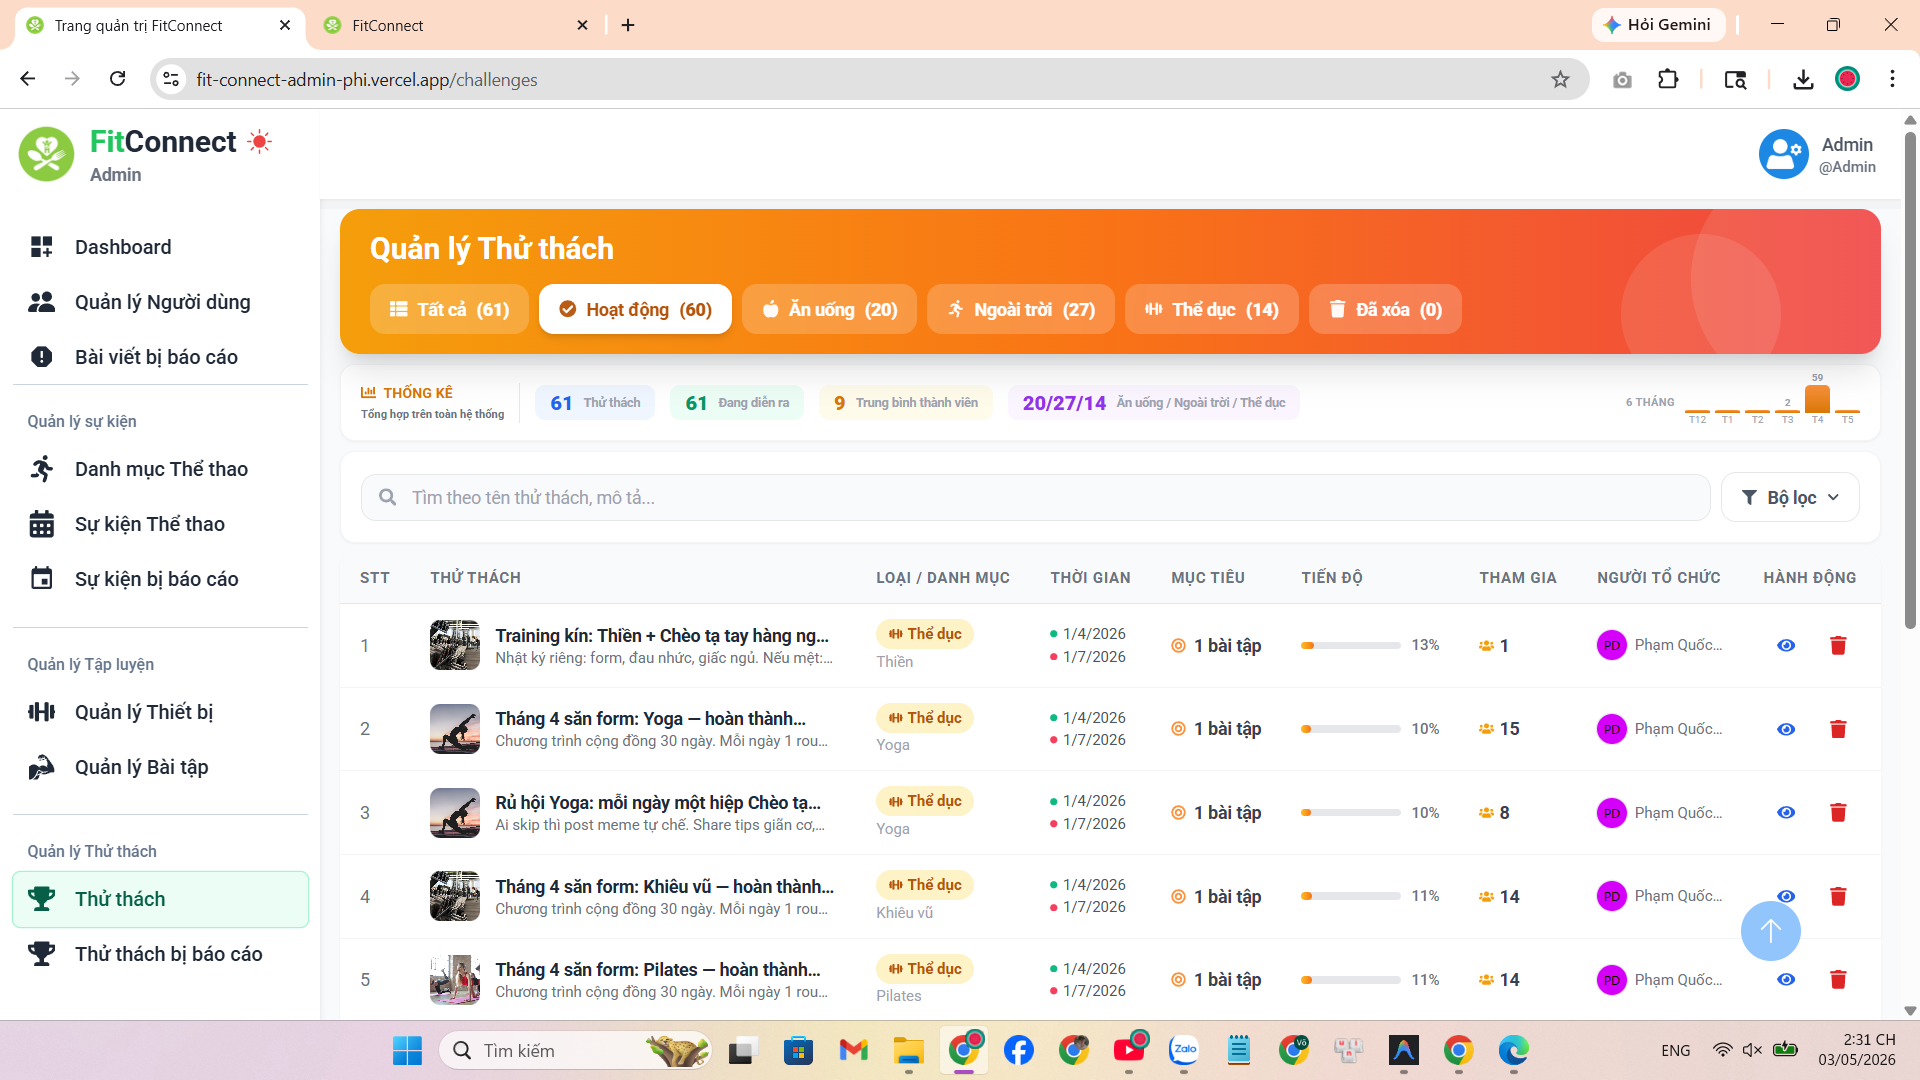
\includegraphics[width=0.60\textwidth]{Images/IMG/nhom9/quanlythuthach/danhsachthuthach.png}
    \caption{Quản trị viên xem danh sách tổng hợp các thử thách trên hệ thống}
    \label{fig:impl_admin_challenge_list}
\end{figure}


    \item Để đánh giá nội dung và tính phù hợp của thử thách, Quản trị viên có thể xem chi tiết thông tin thông qua hộp thoại phân tích. Hệ thống hiển thị đầy đủ mô tả, mục tiêu cần đạt được (ví dụ: số kcal cần đốt, quãng đường cần chạy) và danh sách các bài tập liên quan nếu có.

\begin{figure}[H]
    \centering
    
\includegraphics[width=0.60\textwidth]{Images/IMG/nhom9/quanlythuthach/xemthongtinthuthach.png}
    \caption{Hệ thống hiển thị hộp thoại chi tiết thông tin thử thách}
    \label{fig:impl_admin_challenge_detail}
\end{figure}


    \item Trong quá trình vận hành, nếu phát hiện thử thách có nội dung không phù hợp hoặc vi phạm chính sách nền tảng, Quản trị viên có quyền thực hiện thao tác vô hiệu hóa. Trước khi thực hiện, hệ thống sẽ hiển thị hộp thoại xác nhận để đảm bảo quyết định được cân nhắc kỹ lưỡng.

\begin{figure}[H]
    \centering
    
\includegraphics[width=0.60\textwidth]{Images/IMG/nhom9/quanlythuthach/xoathuthach.png}
    \caption{Hệ thống hiển thị hộp thoại xác nhận vô hiệu hóa thử thách}
    \label{fig:impl_admin_challenge_delete_confirm}
\end{figure}


    \item Sau khi vô hiệu hóa, thử thách chuyển sang chế độ chỉ đọc (người dùng xem được lịch sử nhưng không tương tác thêm). Các thử thách đã xóa được lưu tại kho riêng và có thể khôi phục để người dùng tiếp tục tham gia.

\begin{figure}[H]
    \centering
    \begin{subfigure}[b]{0.47\textwidth}
        \centering
        
\includegraphics[width=\textwidth]{Images/IMG/nhom9/quanlythuthach/danhsachthuthachdaxoa.png}
        \caption{Danh sách thử thách đã vô hiệu hóa}
        \label{fig:impl_admin_challenge_deleted_list}
    \end{subfigure}
    \hfill
    \begin{subfigure}[b]{0.47\textwidth}
        \centering
        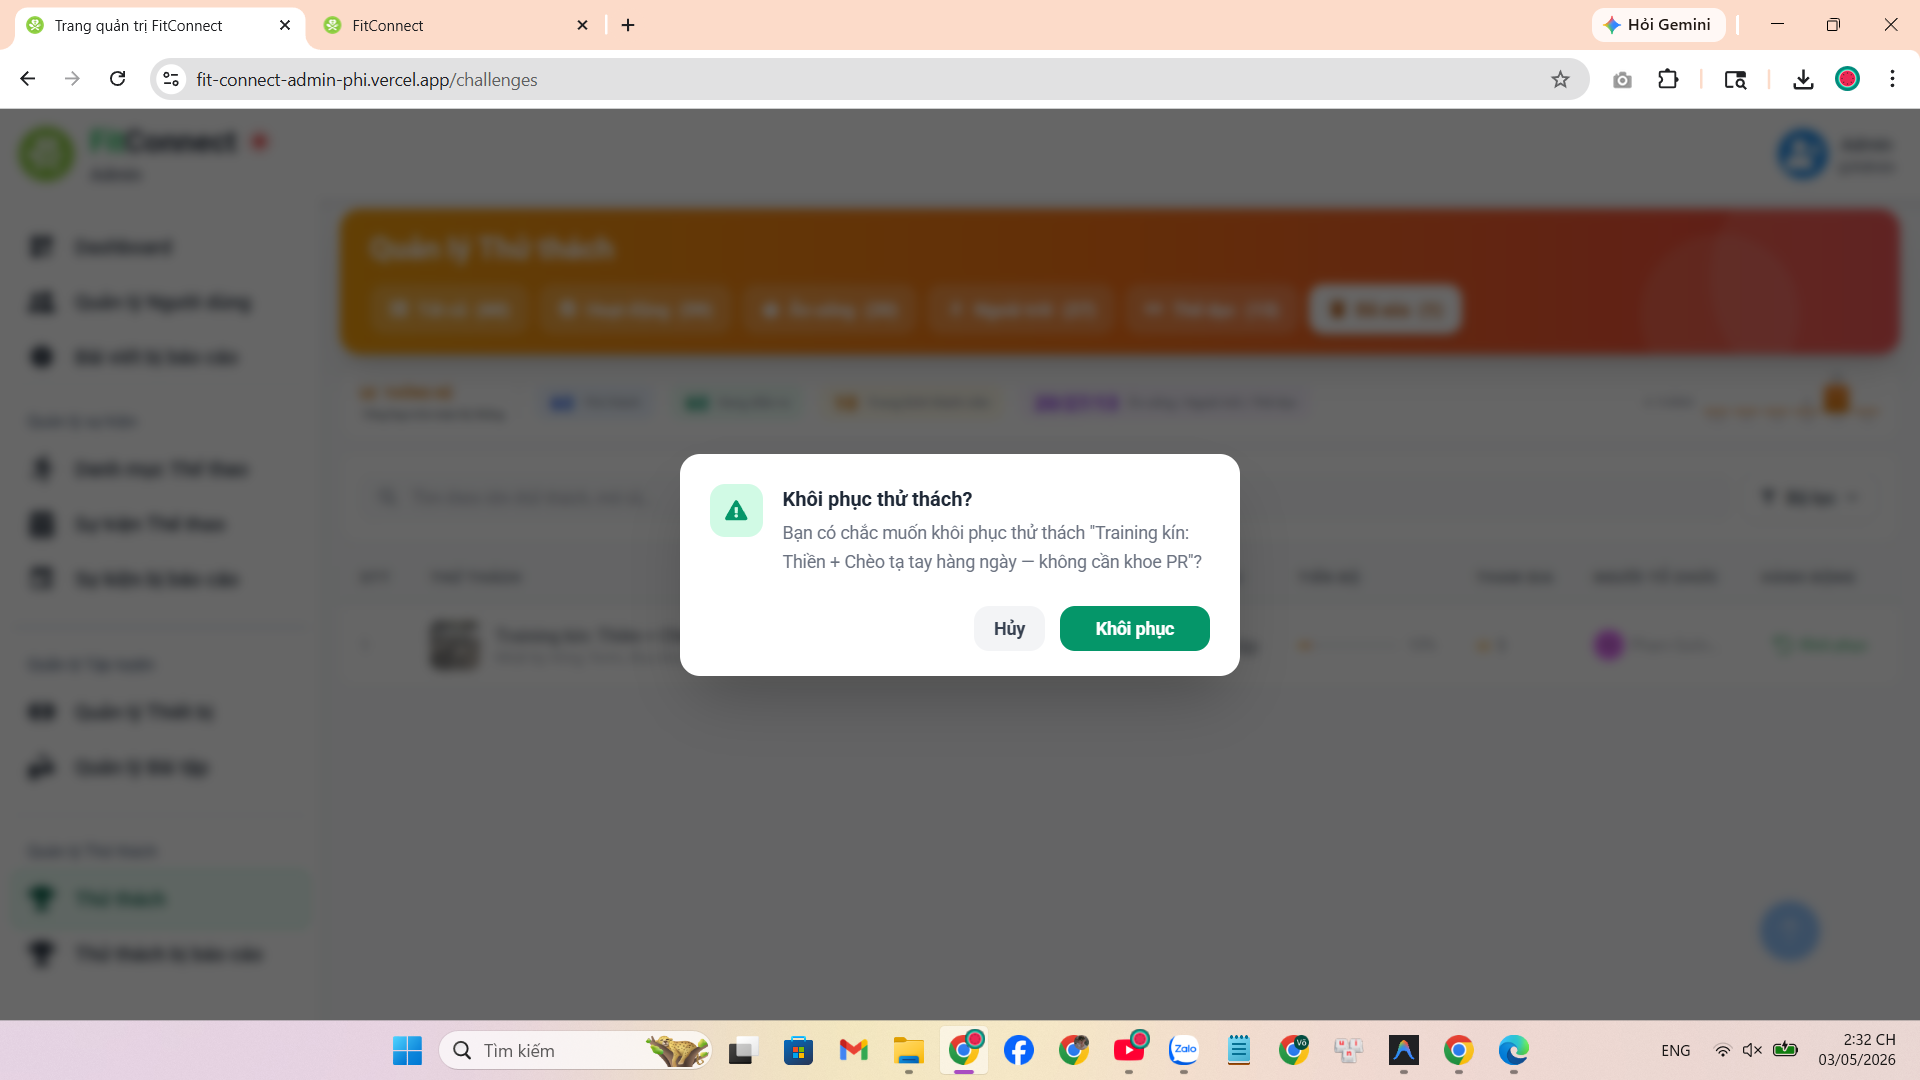
\includegraphics[width=\textwidth]{Images/IMG/nhom9/quanlythuthach/khoiphucthuthach.png}
        \caption{Xác nhận khôi phục thử thách}
        \label{fig:impl_admin_challenge_restore_confirm}
    \end{subfigure}
    \vspace{0.3em}
    \caption{Kho lưu trữ thử thách đã xóa và quy trình khôi phục}
    \label{fig:impl_admin_challenge_trash}
\end{figure}

\end{itemize}

\subsubsection{Luồng thao tác kiểm duyệt Thử thách cộng đồng}
\begin{itemize}
    \item Quy trình kiểm duyệt thử thách bắt đầu từ sự chủ động của cộng đồng người dùng. Khi phát hiện một thử thách có dấu hiệu gian lận, nội dung phản cảm hoặc không phù hợp với tiêu chuẩn sức khỏe, người dùng có thể gửi báo cáo vi phạm trực tiếp kèm theo lý do chi tiết.

\begin{figure}[H]
    \centering
    
\includegraphics[width=0.60\textwidth]{Images/IMG/nhom9/kiemduyetthuthach/baocaothuthach.png}
    \caption{Người dùng thực hiện báo cáo vi phạm đối với một thử thách cộng đồng}
    \label{fig:impl_admin_challenge_mod_report}
\end{figure}


    \item Tại trang quản trị, các thử thách bị báo cáo được tập hợp vào danh sách chờ xử lý. Quản trị viên theo dõi tổng số lượt báo cáo, thông tin người tạo, và nội dung vi phạm bị cáo buộc để ưu tiên xử lý các trường hợp nghiêm trọng.

\begin{figure}[H]
    \centering
    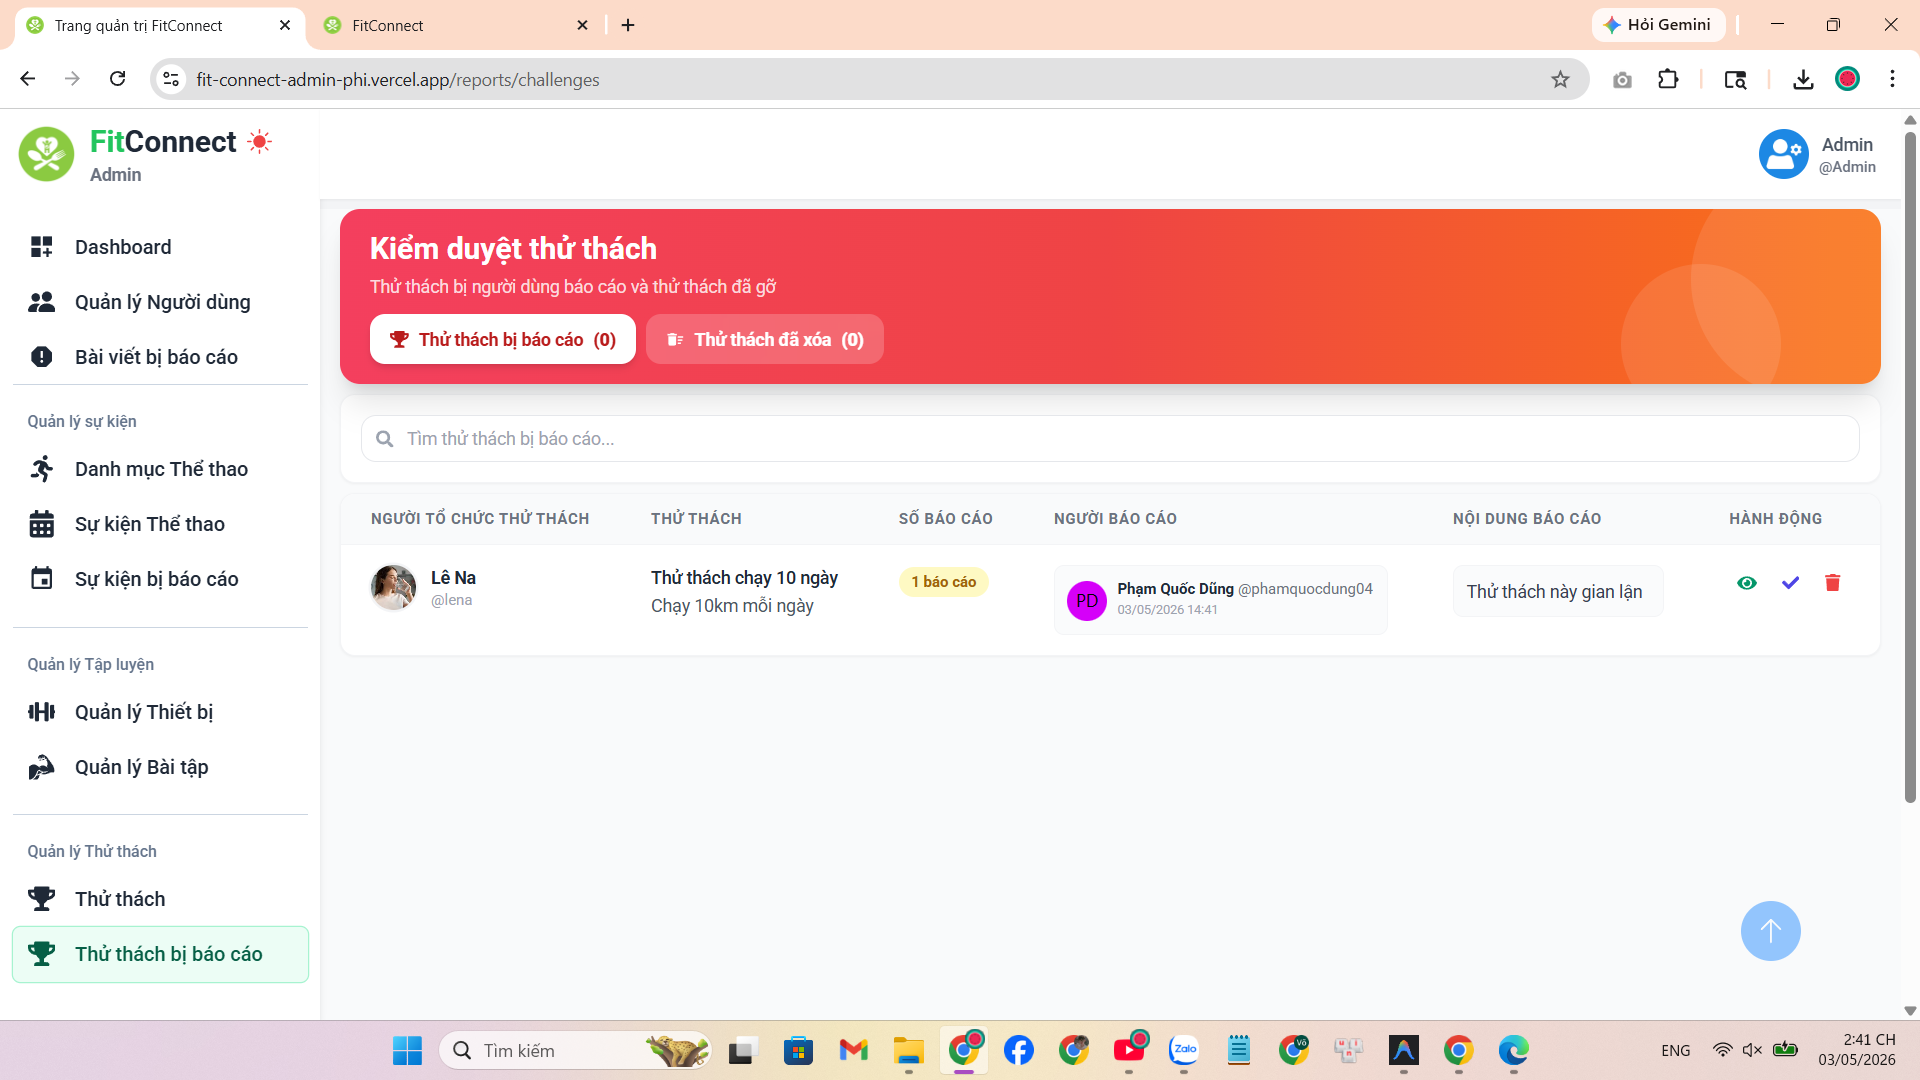
\includegraphics[width=0.60\textwidth]{Images/IMG/nhom9/kiemduyetthuthach/danhsachthuthachbibaocao.png}
    \caption{Quản trị viên theo dõi danh sách các thử thách bị người dùng báo cáo vi phạm}
    \label{fig:impl_admin_challenge_mod_reported_list}
\end{figure}


    \item Để đưa ra quyết định công bằng, Quản trị viên thực hiện xem chi tiết nội dung thử thách cùng với các lý do báo cáo cụ thể từ người dùng thông qua hộp thoại tích hợp.

\begin{figure}[H]
    \centering
    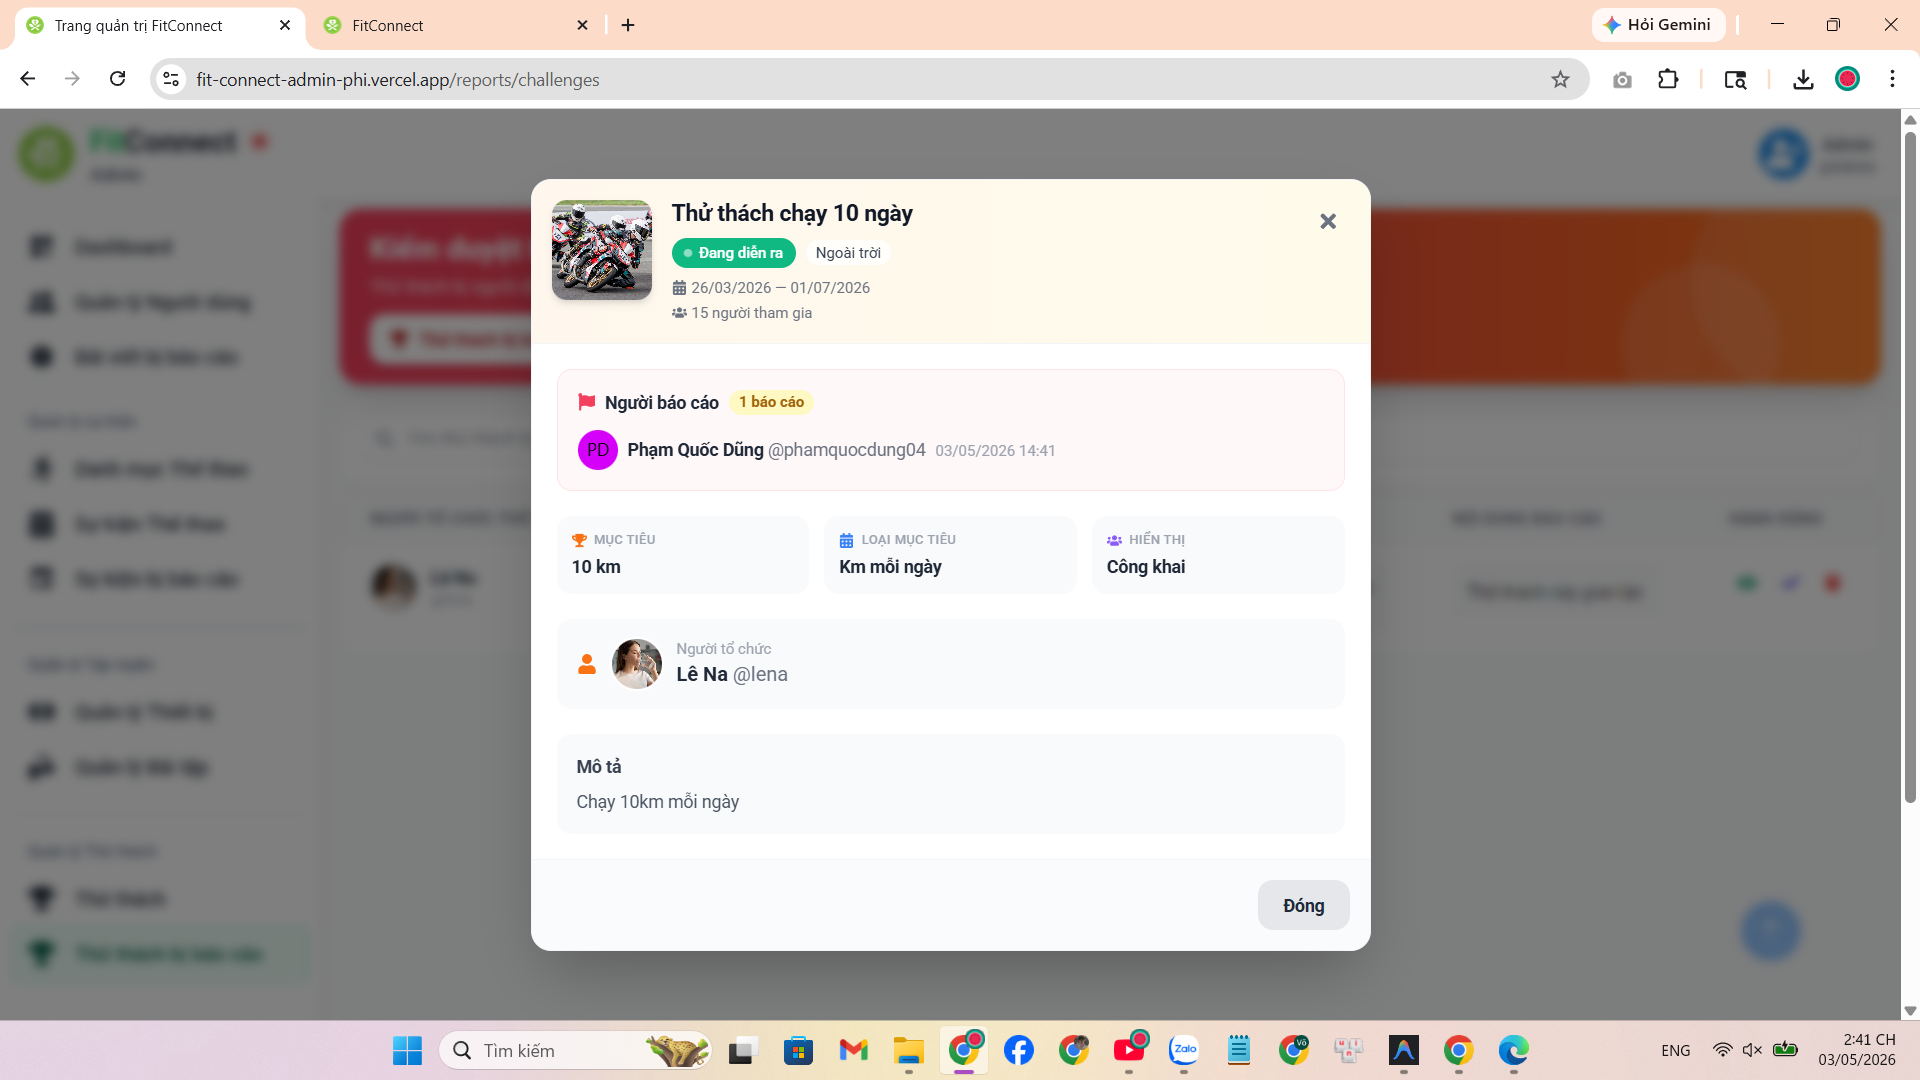
\includegraphics[width=0.60\textwidth]{Images/IMG/nhom9/kiemduyetthuthach/xemthongtinthuthach.png}
    \caption{Hệ thống hiển thị thông tin chi tiết thử thách và các báo cáo liên quan}
    \label{fig:impl_admin_challenge_mod_detail}
\end{figure}


    \item Dựa trên quá trình xác minh, Quản trị viên có hai hướng xử lý chính. Nếu nội dung báo cáo không chính xác, Admin chọn ``Giữ thử thách'' để bác bỏ các báo cáo và duy trì trạng thái hoạt động bình thường. Ngược lại, nếu vi phạm được xác nhận, Admin tiến hành gỡ bỏ thử thách.

\begin{figure}[H]
    \centering
    \begin{subfigure}[b]{0.47\textwidth}
        \centering
        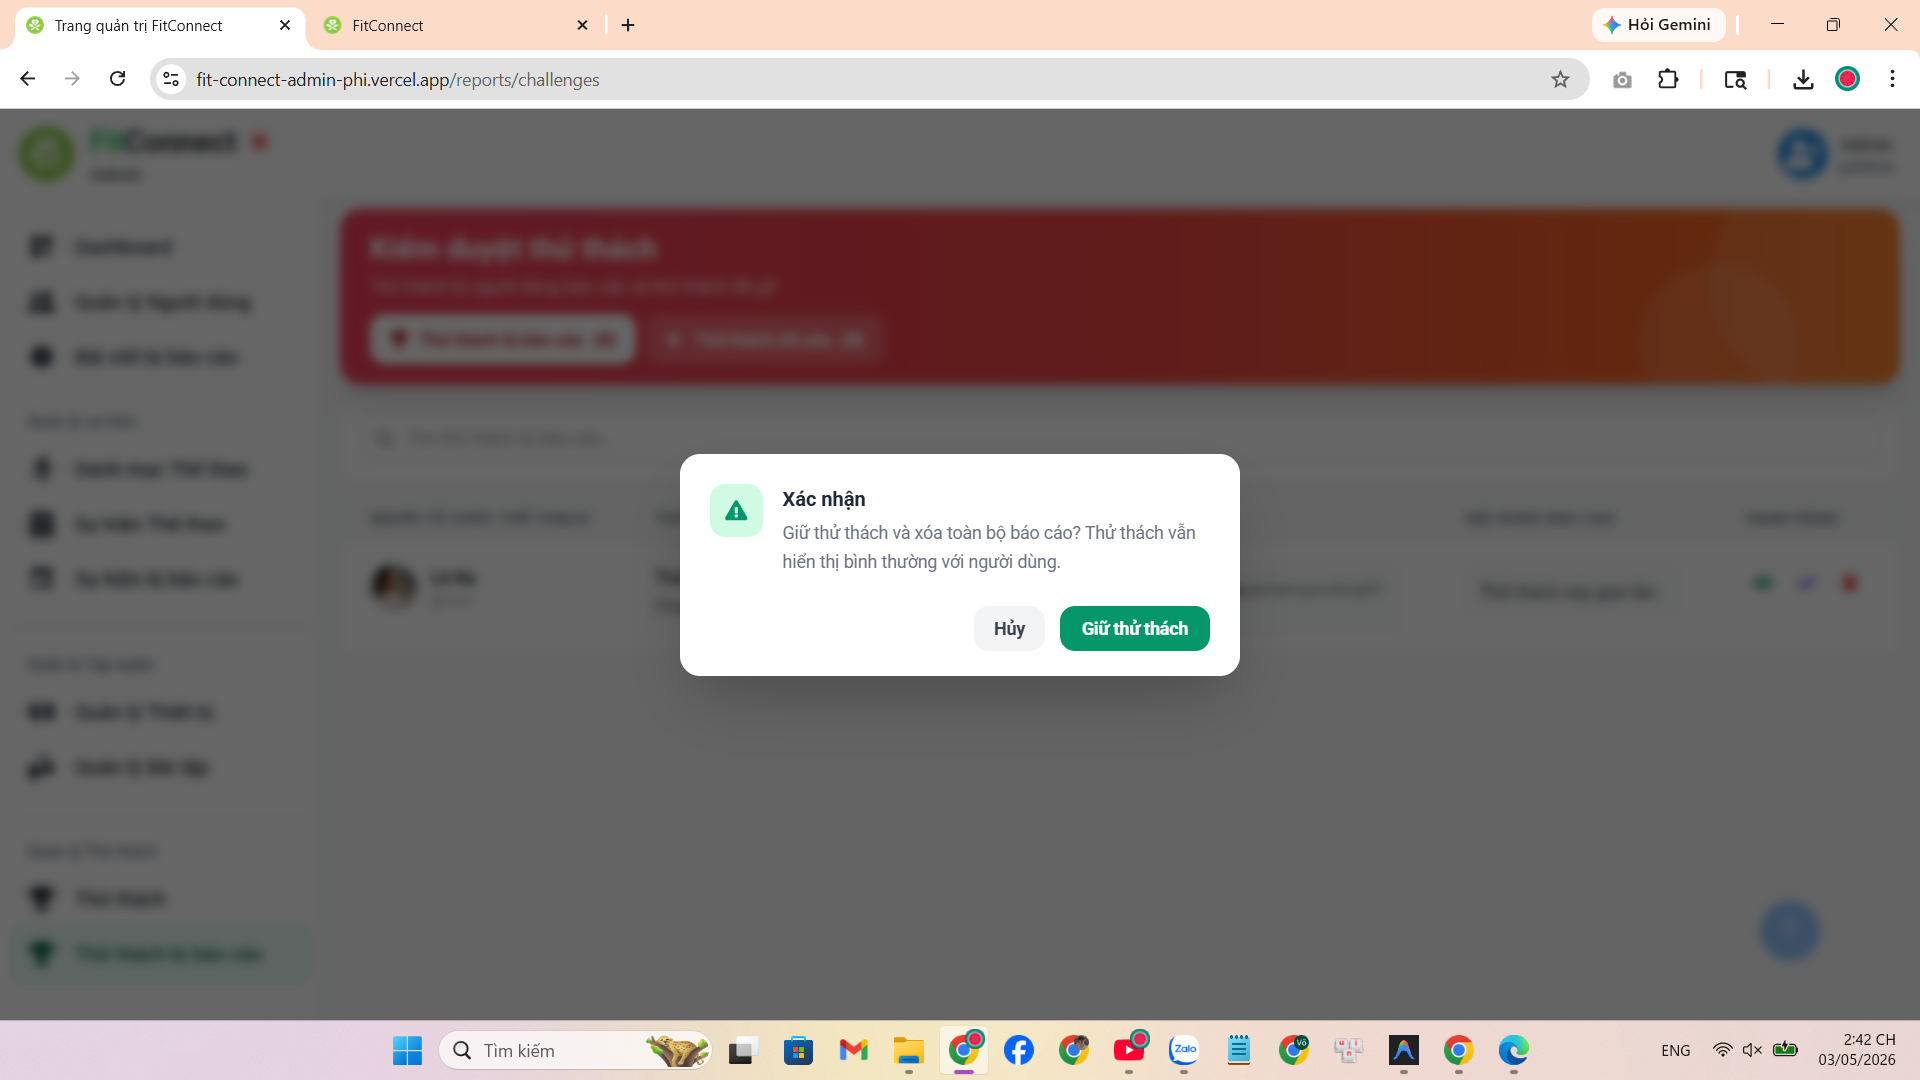
\includegraphics[width=\textwidth]{Images/IMG/nhom9/kiemduyetthuthach/giuthuthach.png}
        \caption{Hộp thoại xác nhận giữ lại thử thách khi báo cáo được xác định là không vi phạm}
        \label{fig:impl_admin_challenge_mod_keep}
    \end{subfigure}
    \hfill
    \begin{subfigure}[b]{0.47\textwidth}
        \centering
        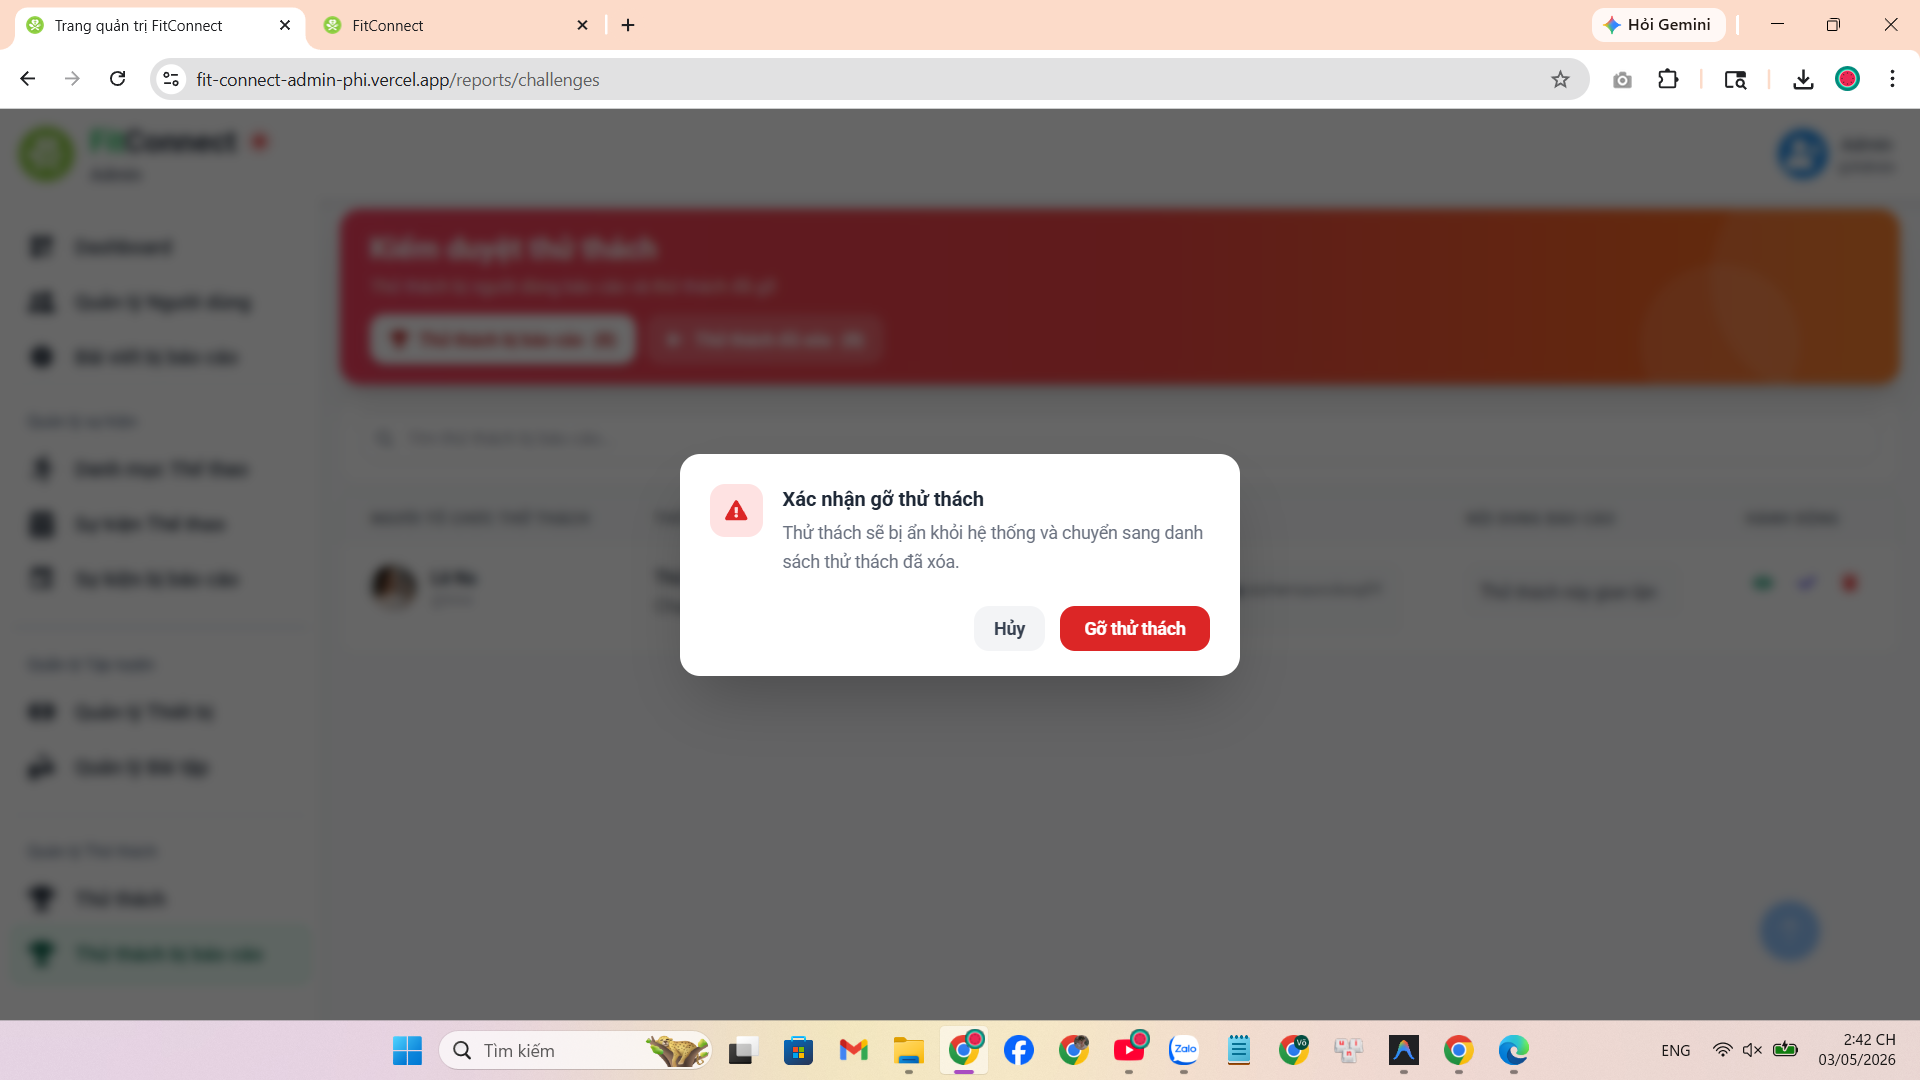
\includegraphics[width=\textwidth]{Images/IMG/nhom9/kiemduyetthuthach/xoathuthach.png}
        \caption{Hệ thống hiển thị hộp thoại xác nhận gỡ bỏ thử thách vi phạm tiêu chuẩn}
        \label{fig:impl_admin_challenge_mod_remove}
    \end{subfigure}
\end{figure}


    \item Thử thách bị gỡ bỏ chuyển sang chế độ chỉ đọc, người dùng không thể tham gia hay cập nhật kết quả mới. Toàn bộ thử thách đã gỡ được lưu tại tab ``Thử thách đã xóa'' và có thể khôi phục nếu cần.

\begin{figure}[H]
    \centering
    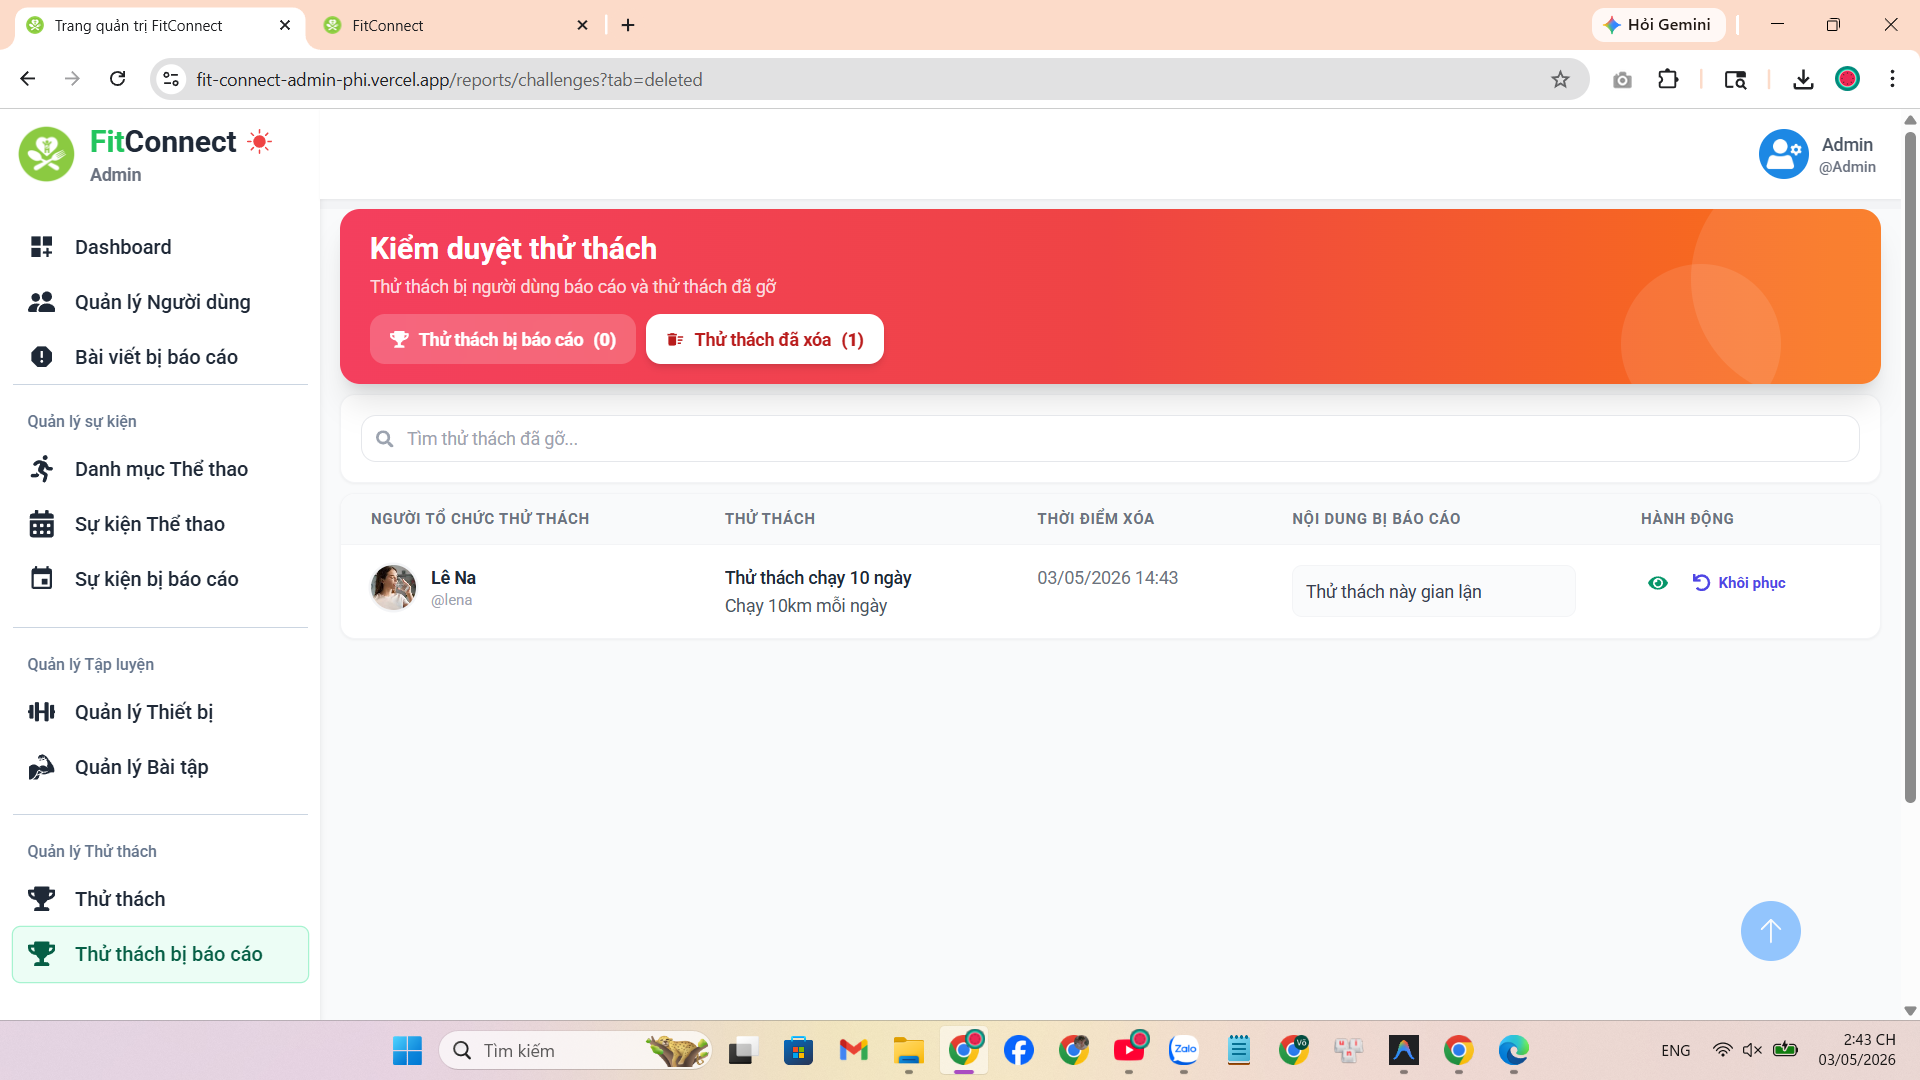
\includegraphics[width=0.60\textwidth]{Images/IMG/nhom9/kiemduyetthuthach/danhsachthuthachdaxoa.png}
    \caption{Danh sách thử thách đã bị gỡ bỏ do vi phạm, cho phép xem xét và khôi phục}
    \label{fig:impl_admin_challenge_mod_deleted_list}
\end{figure}

\end{itemize}

\section{Triển khai và vận hành}
\label{sec:impl_deployment}

Quy trình triển khai và vận hành đóng vai trò quyết định trong việc đưa hệ thống FitConnect từ môi trường phát triển sang môi trường thực tế, đảm bảo tính ổn định, bảo mật và khả năng mở rộng.

\subsection{Cơ sở hạ tầng và Môi trường triển khai}
\label{subsec:impl_infrastructure}

Hệ thống được triển khai trên \textbf{máy chủ VPS Ubuntu} theo sơ đồ Hình~\ref{fig:vps_deploy_diagram} (Chương~\ref{chap:technology}): một điểm vào duy nhất qua \textbf{HTTPS (443)} tới \textbf{Nginx}, vừa kết thúc SSL/TLS, vừa phục vụ file tĩnh và chuyển tiếp API/WebSocket tới tầng ứng dụng.

\begin{itemize}
    \item \textbf{Nginx:} Cấu hình phục vụ thư mục build của \textbf{DATN\_FE} và \textbf{DATN\_ADMIN\_FE} (artefact sau \texttt{npm run build} / Vite thường là \texttt{dist}); đồng thời \texttt{proxy\_pass} các đường dẫn \texttt{/api/...} và \texttt{/socket.io/...} tới tiến trình Node nội bộ.
    \item \textbf{Backend (DATN\_BE):} Chạy trực tiếp trên Node.js (ứng dụng \textbf{Express} tích hợp \textbf{Socket.IO}), được giữ tiến trình bằng \textbf{PM2} để tự khởi động lại khi lỗi và thuận tiện giám sát tài nguyên.
    \item \textbf{Cơ sở dữ liệu:} Có thể dùng \textbf{MongoDB cài trên cùng VPS} hoặc \textbf{MongoDB Atlas} (cloud); ứng dụng kết nối qua biến môi trường \texttt{MONGODB\_URL}.
    \item \textbf{Dịch vụ ngoài (không chạy trên VPS):} \textbf{Cloudinary} (media), \textbf{Goong Maps API} (bản đồ), \textbf{LLM API} (OpenAI-compatible / Groq, Gemini tùy cấu hình) --- Backend gọi ra Internet với khoá bí mật lưu phía server.
\end{itemize}

Việc đóng gói bằng \textbf{Docker} hoặc triển khai Frontend lên nền tảng edge (ví dụ Vercel) vẫn có thể áp dụng trong các biến thể khác, nhưng cấu hình chuẩn của đề tài là \textbf{tập trung trên một VPS} như trên để kiểm soát chi phí và phù hợp môi trường đồ án.

\subsection{Quy trình triển khai (Deployment Workflow)}
\label{subsec:impl_workflow}

Quy trình đưa phiên bản mới lên production trên VPS thường gồm các bước:
\begin{itemize}
    \item \textbf{Quản lý mã nguồn:} Dùng \textbf{Git} và \textbf{GitHub} để phiên bản hóa; trên máy chủ, \texttt{git pull} nhánh ổn định.
    \item \textbf{Build Frontend:} Trong thư mục \texttt{DATN\_FE} và \texttt{DATN\_ADMIN\_FE}, cài dependency (nếu cần), chạy \texttt{npm run build}, đồng bộ thư mục artefact tới đường dẫn mà Nginx đã cấu hình.
    \item \textbf{Build và khởi động Backend:} Trong \texttt{DATN\_BE}, cài dependency, biên dịch TypeScript (\texttt{npm run build} tùy script), khởi động lại bằng \texttt{pm2 restart} (hoặc \texttt{pm2 start} lần đầu).
    \item \textbf{Nginx:} Kiểm tra cú pháp (\texttt{nginx -t}) và \texttt{reload} khi đổi cấu hình server hoặc đường dẫn static.
    \item \textbf{CI/CD (tùy chọn):} Có thể tự động hóa các bước trên bằng GitHub Actions hoặc script SSH; không bắt buộc Docker Registry nếu chạy Node trực tiếp trên VPS.
\end{itemize}

\subsection{Giám sát, Bảo trì và Bảo mật}
\label{subsec:impl_monitoring}

\begin{table}[H]
\centering
\caption{Chiến lược giám sát và bảo mật hệ thống FitConnect}
\label{tab:impl_ops_security}
\small
\renewcommand{\arraystretch}{1.2}
\begin{tabular}{|p{3cm}|p{2.8cm}|p{8.2cm}|}
\hline
\textbf{Lĩnh vực} & \textbf{Công cụ / Cơ chế} & \textbf{Mô tả} \\
\hline
\textbf{Logging} & Winston + Morgan & Ghi nhật ký toàn bộ API request, response và lỗi hệ thống để truy vết sự cố. \\
\hline
\textbf{Monitoring} & PM2 Monit & Theo dõi CPU, RAM của Backend theo thời gian thực; tự động restart khi tiến trình crash. \\
\hline
\textbf{Mã hóa truyền tải} & HTTPS (SSL/TLS) & Toàn bộ dữ liệu giữa Client và Server được mã hóa end-to-end. \\
\hline
\textbf{Xác thực} & JWT + Google OAuth 2.0 & Access Token + Refresh Token đảm bảo phiên an toàn; OAuth 2.0 cho đăng nhập qua Google. \\
\hline
\textbf{Phân quyền} & Middleware checkRole & Tách biệt hoàn toàn route \texttt{/api/admin} khỏi route người dùng thông thường. \\
\hline
\textbf{Phòng thủ ứng dụng} & CORS + Rate Limiting + Bcrypt & Chỉ cho phép domain tin cậy; giới hạn 100 req/15 phút mỗi IP; băm mật khẩu một chiều. \\
\hline
\textbf{Sanitization} & Joi/Yup + DOMPurify & Validate schema đầu vào phía server; lọc XSS/NoSQL Injection trước khi xử lý. \\
\hline
\end{tabular}
\end{table}

\section{Kết luận chương}
\label{sec:impl_conclusion}

Chương 6 đã trình bày toàn bộ quá trình hiện thực hệ thống FitConnect: từ môi trường phát triển, 9 nhóm tính năng cốt lõi, tích hợp AI, đến triển khai và vận hành Production. Hệ thống đã hoàn thiện kiến trúc RESTful API (Node.js + Express), giao diện React với quản lý trạng thái React Query, triển khai trên \textbf{VPS} (Nginx, PM2, HTTPS) kết hợp MongoDB (cục bộ hoặc Atlas), Cloudinary và các API ngoài; bảo mật đa tầng gồm JWT, OAuth 2.0, HTTPS và Rate Limiting. Kết quả này là nền tảng để tiến hành kiểm thử toàn diện ở Chương 7.

